% Sandia National Laboratories is a multimission laboratory managed and
% operated by National Technology & Engineering Solutions of Sandia, LLC, a
% wholly owned subsidiary of Honeywell International Inc., for the U.S.
% Department of Energy’s National Nuclear Security Administration under
% contract DE-NA0003525.

% Copyright 2002-2020 National Technology & Engineering Solutions of Sandia,
% LLC (NTESS).

% When compiling at Sandia, uncomment 'sand' and SANDreport
% Outside of Sandia, uncomment 'report' and scrreprt:
\documentclass[11pt,report]{SANDreport}
\usepackage[sand]{optional}
%\documentclass[11pt,letterpaper]{scrreprt}
%\usepackage[report]{optional}

\usepackage{Xyce}
\usepackage{makeidx,ltxtable, multirow}
\usepackage[hyperindex=true, colorlinks=false]{hyperref}
\usepackage{mdwlist}
\usepackage{float}
\restylefloat{table}
%\usepackage{pdfdraftcopy}
%\draftstring{DRAFT}
% Sandia National Laboratories is a multimission laboratory managed and
% operated by National Technology & Engineering Solutions of Sandia, LLC, a
% wholly owned subsidiary of Honeywell International Inc., for the U.S.
% Department of Energy’s National Nuclear Security Administration under
% contract DE-NA0003525.

% Copyright 2002-2020 National Technology & Engineering Solutions of Sandia,
% LLC (NTESS).


% Macro Definition file for shortening LaTex commands


%Diode equation variables
\newcommand{\bBV}{\mathbf{BV}}
\newcommand{\bIBV}{\mathbf{IBV}}
\newcommand{\bBVeff}{\mathbf{BV_{eff}}}
\newcommand{\bIBVeff}{\mathbf{IBV_{eff}}}
\newcommand{\bIS}{\mathbf{IS}}
\newcommand{\bIRF}{\mathbf{IRF}}
\newcommand{\bN}{\mathbf{N}}

% users guide reference
\newcommand{\UsersGuide}{~\cite{Xyce_Users_Guide_7_1}~}

\newenvironment{Command}
               {\begin{basedescript}{
                     \desclabelstyle{\multilinelabel}
                     \desclabelwidth{1.2in}
                     \renewcommand{\makelabel}[1]{\normalfont\bfseries ##1\hfill}}
                   \def\format{\goodbreak\item[General Form]\ttfamily}
                   \def\examples{\goodbreak\vbox{\hrulefill}\item[Examples]\ttfamily}
                   \def\arguments{\goodbreak\vbox{\hrulefill}\item[Arguments and Options]\normalfont}
                   \def\comments{\goodbreak\vbox{\hrulefill}\item[Comments]\normalfont}
               }
               {\end{basedescript}\normalfont}

\newenvironment{Device}
               {\begin{basedescript}{
                     \desclabelstyle{\multilinelabel}
                     \desclabelwidth{1.2in}
                     \renewcommand{\makelabel}[1]{\normalfont\bfseries ##1\hfill}}
                   \def\symbol{\goodbreak\item[Symbol]\normalfont}
                   \def\device{\goodbreak\vbox{\hrulefill}\item[Instance Form]\ttfamily}
                   \def\model{\goodbreak\vbox{\hrulefill}\item[Model Form]\ttfamily}
                   \def\examples{\goodbreak\vbox{\hrulefill}\item[Examples]\ttfamily}
                   \def\parameters{\goodbreak\vbox{\hrulefill}\item[Parameters and Options]\normalfont}
                   \def\comments{\goodbreak\vbox{\hrulefill}\item[Comments]\normalfont}
               }
               {\end{basedescript}\normalfont}

\newenvironment{Parameters}
               {\vrule height 1pt depth 0pt width 0pt
                 \begin{basedescript}{
                     \desclabelstyle{\nextlinelabel}
                     \desclabelwidth{0.25in}
                     \setlength{\rightmargin}{0.25in}
                     \setlength{\itemindent}{0ex}
                     \setlength{\parsep}{0.5ex plus0.2ex}
                     \setlength{\itemsep}{1ex plus0.2ex}
                   \newcommand\param[1]{\item[\texttt{##1}]}}
               }
               {\end{basedescript}}

\newenvironment{Arguments}
               {\vrule height 1pt depth 0pt width 0pt
                 \begin{basedescript}{
                     \desclabelstyle{\nextlinelabel}
                     \desclabelwidth{0.25in}
                     \renewcommand{\makelabel}[1]{\texttt{##1}\hfill}
                     \setlength{\rightmargin}{0.25in}
                     \setlength{\itemindent}{0ex}
                     \setlength{\parsep}{1ex plus0.2ex}
                     \setlength{\itemsep}{1ex plus0.2ex}
                     \newcommand\argument[1]{\item[##1]}}
               }
               {\end{basedescript}}

\newenvironment{DeviceParamTableGenerated}[2]
               {\renewcommand{\arraystretch}{1.2}
                 \newcommand{\category}[1]{\multicolumn{4}{c}{\smallskip\color{XyceDarkBlue}\em\bfseries ##1}}
                 \begin{longtable}{>{\ttfamily\small}m{2in}<{\normalfont}>{\raggedright\small}m{3in}>{\raggedright\small}m{0.5in}>{\raggedright\let\\\tabularnewline\small}m{0.75in}}
                   \caption{#1}\label{#2} \\ \hline
                   \rowcolor{XyceDarkBlue}
                   \color{white}\normalfont\bf Parameter &
                   \color{white}\bf Description &
                   \color{white}\bf Units &
                   \color{white}\bf Default \endfirsthead
                   \caption[]{#1} \\ \hline
                   \rowcolor{XyceDarkBlue}
                   \color{white}\normalfont\bf Parameter &
                   \color{white}\bf Description &
                   \color{white}\bf Units &
                   \color{white}\bf Default \endhead}
               {\end{longtable}}

\newenvironment{CompositeParamTableGenerated}[2]
               {\renewcommand{\arraystretch}{1.2}
                 \newcommand{\category}[1]{\multicolumn{4}{c}{\smallskip\color{XyceDarkBlue}\em\bfseries ##1}}
                 \begin{longtable}{>{\ttfamily\small}m{2in}<{\normalfont}>{\raggedright\small}m{3in}>{\raggedright\small}m{0.5in}>{\raggedright\let\\\tabularnewline\small}m{0.75in}}
                   \caption{#1}\label{#2} \\ \hline
                   \rowcolor{XyceDarkBlue}
                   \color{white}\normalfont\bf Parameter &
                   \color{white}\bf Description &
                   \color{white}\bf Units &
                   \color{white}\bf Default \endfirsthead
                   \caption[]{#1} \\ \hline
                   \rowcolor{XyceDarkBlue}
                   \color{white}\normalfont\bf Parameter &
                   \color{white}\bf Description &
                   \color{white}\bf Units &
                   \color{white}\bf Default \endhead}
               {\end{longtable}}

\newenvironment{DeviceParamTable}[1]
               {\renewcommand{\arraystretch}{1.2}
                 \newcommand{\category}[1]{\multicolumn{4}{c}{\smallskip\color{XyceDarkBlue}\em\bfseries ##1}}
                 \begin{longtable}{>{\ttfamily\small}m{1in}<{\normalfont}>{\raggedright\small}m{3in}>{\raggedright\small}m{0.5in}>{\raggedright\let\\\tabularnewline\small}m{0.75in}}
                   \caption{#1} \\ \hline
                   \rowcolor{XyceDarkBlue}
                   \color{white}\normalfont\bf Parameter &
                   \color{white}\bf Description &
                   \color{white}\bf Units &
                   \color{white}\bf Default \endfirsthead
                   \caption[]{#1} \\ \hline
                   \rowcolor{XyceDarkBlue}
                   \color{white}\normalfont\bf Parameter &
                   \color{white}\bf Description &
                   \color{white}\bf Units &
                   \color{white}\bf Default \endhead}
               {\end{longtable}}

\newenvironment{ParamTable}[1]
               {\renewcommand{\arraystretch}{1.2}
                 \newcommand{\category}[1]{\multicolumn{4}{c}{\smallskip\color{XyceDarkBlue}\em\bfseries ##1}}
                 \begin{longtable}{>{\ttfamily\small}m{1in}<{\normalfont}>{\raggedright\small}m{3in}>{\raggedright\small}m{0.5in}>{\raggedright\let\\\tabularnewline\small}m{0.75in}}
                   \caption{#1} \\ \hline}
               {\end{longtable}}

\newenvironment{DeviceParamTable4}[2][\empty]
               {\renewcommand{\arraystretch}{1.2}
                 \newcommand{\category}[1]{\multicolumn{5}{c}{\smallskip\color{XyceDarkBlue}\em\bfseries ##1}}
                 \begin{longtable}{>{\ttfamily\small}m{1in}<{\normalfont}>{\raggedright\small}m{3in}>{\raggedright\small}m{0.5in}>{\raggedright\small}m{0.75in}>{\raggedright\let\\\tabularnewline\small}m{0.75in}}
                   \ifx\empty#1\caption{#2} \else \caption[#1]{#2}\fi
                    \\ \hline
                   \rowcolor{XyceDarkBlue}
                   \color{white}\normalfont\bf Parameter &
                   \color{white}\bf Description &
                   \color{white}\bf Units &
                   \color{white}\bf Default &
                   \color{white}\bf Device Type \endfirsthead
                   \caption[]{#2} \\ \hline
                   \rowcolor{XyceDarkBlue}
                   \color{white}\normalfont\bf Parameter &
                   \color{white}\bf Description &
                   \color{white}\bf Units &
                   \color{white}\bf Default &
                   \color{white}\bf Device Type \endhead}
               {\end{longtable}}

\newenvironment{OptionTable}[1]
               {\renewcommand{\arraystretch}{1.2}
                 \begin{longtable}[hb]{>{\ttfamily\small}m{1.2in}<{\normalfont}>{\raggedright\small}m{3.5in}>{\raggedright\let\\\tabularnewline\small}m{0.75in}}
                   \caption{#1} \\ \hline
                   \rowcolor{XyceDarkBlue}
                   \color{white}\normalfont\bf Option &
                   \color{white}\bf Description &
                   \color{white}\bf Default \endfirsthead
                   \caption[]{#1} \\ \hline
                   \rowcolor{XyceDarkBlue}
                   \color{white}\normalfont\bf Option &
                   \color{white}\bf Description &
                   \color{white}\bf Default \endhead}
               {\end{longtable}}

\newenvironment{OptionTable4}[1]
               {\renewcommand{\arraystretch}{1.2}
                 \begin{longtable}[hb]{>{\ttfamily\small}m{1.2in}<{\normalfont}>{\raggedright\small}m{3.5in}>{\small}m{0.75in}>{\raggedright\let\\\tabularnewline\small}m{0.75in}}
                   \caption{#1} \\ \hline
                   \rowcolor{XyceDarkBlue}
                   \color{white}\normalfont\bf Option &
                   \color{white}\bf Description &
                   \color{white}\bf NONLIN Default &
                   \color{white}\bf NONLIN-TRAN Default \endfirsthead
                   \caption[]{#1} \\ \hline
                   \rowcolor{XyceDarkBlue}
                   \color{white}\normalfont\bf Option &
                   \color{white}\bf Description &
                   \color{white}\bf NONLIN Default &
                   \color{white}\bf NONLIN-TRAN Default \endhead}
               {\end{longtable}}

\def\debug{\cellcolor[gray]{0.75}}

% Xyce_RG_macros includes some ``short-hand'' definitions to not have to type
% so much stuff out explicitly!

\opt{report}{
     \usepackage{fullpage}
     \DeclareOldFontCommand{\rm}{\normalfont\rmfamily}{\mathrm}
     \DeclareOldFontCommand{\sf}{\normalfont\sffamily}{\mathsf}
     \DeclareOldFontCommand{\tt}{\normalfont\ttfamily}{\mathtt}
     \DeclareOldFontCommand{\bf}{\normalfont\bfseries}{\mathbf}
     \DeclareOldFontCommand{\it}{\normalfont\itshape}{\mathit}
     \DeclareOldFontCommand{\sl}{\normalfont\slshape}{\@nomath\sl}
     \DeclareOldFontCommand{\sc}{\normalfont\scshape}{\@nomath\sc}
}

\includeonly{
acktrade,
Xyce_RG_ch01,
Xyce_RG_app1,
Xyce_RG_PDE,
Xyce_RG_app2,
Xyce_RG_app_rawformat,
Xyce_RG_dist
}

%\draft

\makeindex

% ---------------------------------------------------------------------------- %
%
% Set the title, author, and date
%
%Submitted to R&A TBD May 2020, Tracking number TBD, approved TBD May 2020
\title{\XyceTitle{} Parallel Electronic Simulator\\Reference Guide, Version 7.1}
\author{Eric R. Keiter,
            Thomas V. Russo,
            Richard L. Schiek,\\
            Heidi K. Thornquist,
            Ting Mei,
            Jason C. Verley\\
            Peter E. Sholander,
            Karthik V. Aadithya
}
\date{}

% ---------------------------------------------------------------------------- %
% Set some things we need for SAND reports. These are mandatory
%
\opt{sand}{
\SANDnum{SAND2020-TBD}
\SANDprintDate{May 2020}
\SANDauthor{Eric R. Keiter, Thomas V. Russo, Richard L. Schiek, Heidi K.  Thornquist,\\%
     Ting Mei, Jason C. Verley, Peter E. Sholander, Karthik V. Aadithya}
}

\begin{document}

% Set to roman page numbers for front matter
%\pagenumbering{roman}

\maketitle

\opt{report}{
\noindent
Issued by Sandia National Laboratories, operated for the United States
Department of Energy by National Technology \& Engineering Solutions of Sandia,
LLC.\\
\\
NOTICE:  This report was prepared as an account of work sponsored by an agency
of the United States Government. Neither the United States Government, nor any
agency thereof, nor any of their employees, nor any of their contractors,
subcontractors, or their employees, make any warranty, express or implied, or
assume any legal liability or responsibility for the accuracy, completeness, or
usefulness of any information, apparatus, product, or process disclosed, or
represent that its use would not infringe privately owned rights. Reference
herein to any specific commercial product, process, or service by trade name,
trademark, manufacturer, or otherwise, does not necessarily constitute or imply
its endorsement, recommendation, or favoring by the United States Government,
any agency thereof, or any of their contractors or subcontractors. The views
and opinions expressed herein do not necessarily state or reflect those of the
United States Government, any agency thereof, or any of their contractors.
\vfill
\noindent
Sandia National Laboratories is a multimission laboratory managed and operated
by National Technology \& Engineering Solutions of Sandia, LLC, a wholly owned
subsidiary of Honeywell International Inc., for the U.S.  Department of
Energy’s National Nuclear Security Administration under contract DE-NA0003525.
}

\begin{abstract}

This document is a reference guide to the \Xyce{} Parallel Electronic
Simulator, and is a companion document to the \Xyce{} Users' Guide\UsersGuide.
The focus of this document is (to the extent
possible) exhaustively list device parameters, solver options, parser
options, and other usage details of \Xyce{}.  This document is \emph{not}
intended to be a tutorial.  Users who are new to circuit simulation are 
better served by the \Xyce{} Users' Guide\UsersGuide.

\end{abstract}

\clearpage

% acknowledgements, trademarks, contact information.
% Sandia National Laboratories is a multimission laboratory managed and
% operated by National Technology & Engineering Solutions of Sandia, LLC, a
% wholly owned subsidiary of Honeywell International Inc., for the U.S.
% Department of Energy’s National Nuclear Security Administration under
% contract DE-NA0003525.

% Copyright 2002-2021 National Technology & Engineering Solutions of Sandia,
% LLC (NTESS).

%%-------------------------------------------------------------------------
%% Acknowledgements, Trademarks, and contact information for the Xyce
%% project.

\chapter*{Acknowledgments}

We would like to acknowledge all the code and test suite developers who have
contributed to the Xyce project over the years: 
Aaron Gibson,
Alan Lundin,
Antonio Gonzales,
Ashley Meek,
Bart van Bloemen Waanders,
Brad Bond,
Brian Fett,
Christina Warrender,
David Baur,
David Day,
David Shirley,
Deborah Fixel,
Derek Barnes,
Eric Rankin,
Erik Zeek,
Gary Hennigan,
Herman "Buddy" Watts,
Jim Emery,
Jonathan Woodbridge,
Jonathen Kwok,
Keith Santarelli,
Laura Boucheron,
Lawrence Musson,
Lon Waters,
Mary Meinelt,
Michael Skoufis,
Mingyu \mbox{"Genie"} Hsieh,
Nicholas Johnson,
Philip Campbell,
Rachel Campbell,
Randall Lober,
Rebecca Arnold,
Regina Schells,
Richard Drake,
Robert Hoekstra,
Roger Pawlowski,
Russell Hooper,
Samuel Browne,
Scott Hutchinson,
Simon Zou,
Smitha Sam,
Steven Verzi,
Tamara Kolda,
Timur Takhtaganov, and
Todd Coffey.

\noindent
Also, thanks to Hue Lai for the original typesetting of this document in \LaTeX.

\subsection*{Trademarks}

\Xyce{} Electronic Simulator\textsuperscript{\scriptsize{\texttrademark}} and
\XyceTM{} are trademarks of National Technology \& Engineering Solutions of
Sandia, LLC (NTESS).

\subsection*{Contact Information} \label{Contact Information}

\begin{flushright}
Address \hfill Electrical Models \& Simulation Dept.\\
     Sandia National Laboratories\\
     P.O. Box 5800, MS 1177\\
     Albuquerque, NM 87185-1177 \\
\end{flushright}

\noindent
\textbf{Outside Sandia}\\
World Wide Web \hfill 
  \texttt{\color{XyceDeepRed}http://xyce.sandia.gov}
\\
Email \hfill
  \texttt{\color{XyceDeepRed}xyce@sandia.gov}
\\

\noindent
\textbf{Inside Sandia}\\
World Wide Web \hfill 
  \texttt{\color{XyceDeepRed}https://infod-ng.sandia.gov/xyce/}
\\
Email \hfill
  \texttt{\color{XyceDeepRed}xyce-sandia@sandia.gov}

\vfill
\noindent
\parbox{\textwidth}{
     \parbox{4.1in}{\small This document is copyright \textcopyright{}
     2002-2021 National Technology \&\\Engineering Solutions of Sandia, LLC.}
     \hfill
     
\includegraphics[height=0.75in]{xyce_flat_white}
}



\cleardoublepage
\pdfbookmark[1]{Table of Contents}{TOC}
\tableofcontents

\cleardoublepage
\pdfbookmark[1]{List of Figures}{LOF}
\listoffigures

\cleardoublepage
\pdfbookmark[1]{List of Tables}{LOT}
\listoftables

\cleardoublepage

\opt{sand}{
\SANDmain
}

% Sandia National Laboratories is a multimission laboratory managed and
% operated by National Technology & Engineering Solutions of Sandia, LLC, a
% wholly owned subsidiary of Honeywell International Inc., for the U.S.
% Department of Energy’s National Nuclear Security Administration under
% contract DE-NA0003525.

% Copyright 2002-2020 National Technology & Engineering Solutions of Sandia,
% LLC (NTESS).


\chapter{Introduction}
\label{Introduction}

\chapteroverview{Welcome to \XyceTitle{}}
{
The \XyceTM{} Parallel Electronic Simulator has been written to support, in a
rigorous manner, the simulation needs of the Sandia National Laboratories
\index{Sandia National Laboratories} electrical designers.  It is targeted 
specifically to run on large-scale parallel computing
\index{parallel!computing} platforms but also runs well on a variety
of architectures including single processor workstations.  It also aims to
support a variety of devices and models specific to Sandia needs.
}
\section{Overview}
\label{Overview}

This document is intended to complement the \Xyce{} Users' 
Guide\UsersGuide.  It contains comprehensive, detailed
information about a number of topics pertinent to the usage of \Xyce{}.  
Included in this document is a
netlist reference for the input-file commands and elements supported 
within \Xyce{}; a command line reference, which describes the 
available command line arguments for \Xyce{}; and quick-references for 
users of other circuit codes, such as Orcad's PSpice~\cite{PSpiceUG:1998}.

\section{How to Use this Guide}
\label{HowTo_Guide}

This guide is designed so you can quickly find the information you need to 
use \Xyce{}.  It assumes that you are familiar with basic Unix-type 
commands, how \index{Unix}Unix manages applications and files to 
perform routine tasks (e.g., starting applications, opening files and 
saving your work).  Note that while Windows versions of \Xyce{} are 
available, they are command-line programs meant to be run under the 
\emph{Command Prompt}, and are used almost identically to their Unix counterparts.

\section{Typographical conventions}
Before continuing in this Reference Guide, it is important to understand 
the terms and typographical conventions used.  Procedures for performing 
an operation are generally indicated with the following typographical 
conventions.

\begin{table}[htbp]
  \caption{\Xyce{} typographical conventions.}
  \begin{tabularx}{\linewidth}{|Y|Y|Y|}
    \rowcolor{XyceDarkBlue} \color{white}\bf Notation & \color{white}\bf
    Example & \color{white}\bf Description \\ \hline

    \texttt{Typewriter text} & \texttt{mpirun -np 4}
    & Commands entered
    from the keyboard on the command line or text entered in a netlist. \\
    \hline

    \textrmb{Bold Roman Font} & Set nominal temperature using the
    \textrmb{TNOM} option. & SPICE-type parameters used in models, etc. \\
    \hline

    \cellcolor[gray]{0.75} Gray Shaded Text & \cellcolor[gray]{0.75} DEBUGLEVEL
    & Feature that is designed primarily for use by \Xyce{}
    developers. \\ \hline

    \texttt{[text in brackets]} & \texttt{Xyce [options] <netlist>} & Optional parameters. \\ \hline

    \texttt{<text in angle brackets>} & \texttt{Xyce [options] <netlist>} &
    Parameters to be inserted by the user. \\ \hline

    \texttt{<object with asterisk>*} & \texttt{K1 <ind. 1> [<ind. n>*]} &
    Parameter that may be multiply specified. \\ \hline

    \texttt{<TEXT1|TEXT2>}&
    \texttt{.PRINT TRAN}
    \verb-+     DELIMITER=<TAB|COMMA>- & Parameters that may only take specified values. \\ \hline

  \end{tabularx}
\end{table}


\cleardoublepage
% Sandia National Laboratories is a multimission laboratory managed and
% operated by National Technology & Engineering Solutions of Sandia, LLC, a
% wholly owned subsidiary of Honeywell International Inc., for the U.S.
% Department of Energy’s National Nuclear Security Administration under
% contract DE-NA0003525.

% Copyright 2002-2021 National Technology & Engineering Solutions of Sandia,
% LLC (NTESS).


\chapter{Netlist Reference}
\label{Netlist_Reference}
\index{netlist!reference}

\chapteroverview{Chapter Overview}
{
This chapter contains reference material directed towards working with circuit
analyses in \Xyce{} using the netlist interface.  Included are
detailed command descriptions, start-up option definitions and a list of
devices supported by the \Xyce{} netlist interface.
}

\section{Netlist Commands}
\label{Netlist_Commands}
\index{netlist!commands}

This section outlines the netlist commands that can be used with \Xyce{} to
setup and control circuit analysis.

%%%%%%%%%%%%%%%%%%%%%%%%%%%%%%%%%%%%%%%%%%%%%%%%%%%%%%%%%%%%%%%%%%%%%%%%%%%%%%%%
%%\newpage
\subsection{\texttt{.AC} (AC Analysis) }
\index{\texttt{.AC}}
\index{analysis!AC} \index{AC analysis}
% Sandia National Laboratories is a multimission laboratory managed and
% operated by National Technology & Engineering Solutions of Sandia, LLC, a
% wholly owned subsidiary of Honeywell International Inc., for the U.S.
% Department of Energy’s National Nuclear Security Administration under
% contract DE-NA0003525.

% Copyright 2002-2020 National Technology & Engineering Solutions of Sandia,
% LLC (NTESS).


Calculates the frequency response of a circuit over a range of frequencies.

The .AC command can specify a linear sweep, decade logarithmic sweep,
octave logarithmic sweep, or a data table of multivariate values.

\begin{Command}

\format
\begin{alltt}
.AC <sweep type> <points value>
+ <start frequency value> <end frequency value>
\end{alltt}

\examples
\begin{alltt}
.AC LIN 101 100Hz 200Hz
.AC OCT 10 1kHz 16kHz
.AC DEC 20 1MEG 100MEG
.AC DATA=<table name>
\end{alltt}

\arguments

\begin{Arguments}

\argument{sweep type}
Must be \texttt{LIN}, \texttt{OCT}, \texttt{DEC}, or \texttt{DATA} as described below.
\begin{description}

\item[\tt LIN] Linear sweep\\
The sweep variable is swept linearly from the starting to the ending value.

\item[\tt OCT] Sweep by octaves\\
The sweep variable is swept logarithmically by octaves.

\item[\tt DEC] Sweep by decades\\
The sweep variable is swept logarithmically by decades.

\item[\tt DATA] Sweep values from a table\\
Sweep variables are applied based on the rows of a data table.  This format allows magnitude and phase to be swept in addition to frequency.    If using this format, no other arguments are needed on the \texttt{.AC} line.

\end{description}

\argument{points value}
Specifies the number of points in the sweep, using an integer greater than or equal to 1.

\argument{\vbox{\hbox{start frequency value\hfil}\hbox{end frequency value}}}

The end frequency value must not be less than the start frequency value,
and both must be greater than zero. The whole sweep must include at
least one point.

\end{Arguments}

\comments

AC analysis is a linear analysis. The simulator calculates the frequency
response by linearizing the circuit around the DCOP bias point.

If specifying the sweep points using the \texttt{DATA} type, one can
also sweep the magnitude and phase of an AC source, as well as the
values of linear model parameters.  However, unlike the use of
\texttt{DATA} for \texttt{.STEP} and \texttt{.DC}, it is not possible
to sweep nonlinear device parameters.  This is because changing other
nonlinear device parameters would alter the correct DCOP solution, and
the AC sweep happens after the DCOP calculation in the analysis flow.
To sweep a nonlinear device parameter on an AC problem, add a
\texttt{.STEP} command to the netlist to provide an outer parametric
sweep around the analysis.

\index{\texttt{.PRINT}}\index{results!print}\index{\texttt{.PRINT}!\texttt{AC}}
A \texttt{.PRINT AC} must be used to get the results of the AC sweep
analysis.  See Section \ref{.PRINT}.

Some devices that may be expected to work in AC analysis do not at
this time.  This includes, but is not limited to, the lossy
transmission line (LTRA) and lossless transmission line (TRA).  The
LTRA and TRA models will need to be replaced with lumped transmission
line models (YTRANSLINE).

Power calculations (\texttt{P(<device>)} and \texttt{W(<device>}) are
not supported for any devices for AC analysis.  Current variables
(e.g., \texttt{I(<device>)}) are only supported for devices that have
``branch currents'' that are part of the solution vector. This
includes the V, E, H and L devices.  It also includes the voltage-form
of the B device.

\end{Command}


%%%%%%%%%%%%%%%%%%%%%%%%%%%%%%%%%%%%%%%%%%%%%%%%%%%%%%%%%%%%%%%%%%%%%%%%%%%%%%%%
\newpage
\subsection{\texttt{.DATA} (Data Table for sweeps) }
\index{\texttt{DATA}}
% Sandia National Laboratories is a multimission laboratory managed and
% operated by National Technology & Engineering Solutions of Sandia, LLC, a
% wholly owned subsidiary of Honeywell International Inc., for the U.S.
% Department of Energy’s National Nuclear Security Administration under
% contract DE-NA0003525.

% Copyright 2002-2021 National Technology & Engineering Solutions of Sandia,
% LLC (NTESS).


User-defined data table, which can be used to specify sweep points for \texttt{.AC}, \texttt{.DC}, \texttt{.NOISE} or \texttt{.STEP}

\begin{Command}

\format
.DATA [<name>] \\
+ <parameter name> [parameter name]* \\
+ <parameter value> [parameter value]* \\
.ENDDATA

\examples
.data test \\
+ r1   r2 \\
+ 8.0000e+00  4.0000e+00 \\
+ 9.0000e+00  4.0000e+00 \\
.enddata

\arguments

\begin{Arguments}
\argument{name}
Name of the data table.

\argument{parameter name}
Name of sweep parameter.  This can be a device instance parameter, a device model parameter or a global parameter specified using \texttt{.global\_param}.

\argument{parameter value}
Value of sweep parameter for the given sweep point.  This must be a double precision number.  Each row of the table corresponds to a different sweep step, so multiple parameters can be changed simultaneously.

\end{Arguments}

\comments

Each column of a data table corresponds to a different parameter, and each row corresponds to a different sweep point.

If using \texttt{.DATA} with \texttt{.DC} or \texttt{.STEP}, then any instance parameter, model parameter, or global parameter is allowed.

However, if using \texttt{.DATA} with \texttt{.AC} or \texttt{.NOISE}, then one can sweep the magnitude and phase of an AC source, and linear model parameters (such as resistance and capacitance) in addition to the traditional AC sweep variable, frequency.  Parameters associated with nonlinear models (like transistors) are not allowed.  This is because AC analysis is a linear analysis, performed after the DCOP calculation.  Changing nonlinear device model parameters would result in a different DCOP solution, so changing them during the AC (or NOISE) analysis phase is not valid.

Another caveat, for both \texttt{.AC} and \texttt{.NOISE}, is that all of the frequency
values in the data table must be positive.  If \texttt{.DATA} is used with \texttt{.NOISE}
then the integrals for the total input noise and total output noise will only be calculated,
and sent to stdout, if the frequencies in the data table are monotonically increasing.

\end{Command}


%%%%%%%%%%%%%%%%%%%%%%%%%%%%%%%%%%%%%%%%%%%%%%%%%%%%%%%%%%%%%%%%%%%%%%%%%%%%%%%%
\newpage
\subsection{\texttt{.DC} (DC Sweep Analysis) }
\index{\texttt{DC}}
\index{analysis!DC} \index{DC analysis}
% Sandia National Laboratories is a multimission laboratory managed and
% operated by National Technology & Engineering Solutions of Sandia, LLC, a
% wholly owned subsidiary of Honeywell International Inc., for the U.S.
% Department of Energy’s National Nuclear Security Administration under
% contract DE-NA0003525.

% Copyright 2002-2020 National Technology & Engineering Solutions of Sandia,
% LLC (NTESS).


Calculates the operating point\index{Operating Point} for the circuit for a
range of values.  Primarily, this capability is applied to independent
voltage sources, but it can also be applied to most device parameters.
Note that this may be repeated for multiple sources in the
same \texttt{.DC} line.

The .DC command can specify a linear sweep, decade logarithmic sweep,
octave logarithmic sweep, a list of values, or a data table of multivariate values.

\subsubsection{Linear Sweeps}
\index{analysis!DC!Linear sweeps} \index{DC analysis!Linear sweeps}

\begin{Command}
\format
\begin{alltt}
.DC [LIN] <sweep variable name> <start> <stop> <step>
+ [<sweep variable name> <start> <stop> <step>]*
\end{alltt}

\examples
\begin{alltt}
.DC LIN V1 5 25 5
.DC VIN -10 15 1
.DC R1 0 3.5 0.05 C1 0 3.5 0.5
\end{alltt}

\comments
A \texttt{.PRINT DC} must be used to get the results of the DC sweep
analysis.  See Section \ref{.PRINT}.
\index{\texttt{.PRINT}}\index{results!print}\index{\texttt{.PRINT}!\texttt{DC}}

A \texttt{.OP} comand will result in a linear DC analysis if there is no .DC specified.

If the stop value is smaller than the start value, the step value
should be negative.  If a positive step value is given in this case,
only a single point (at the start value) will be performed, and a
warning will be emitted.

\end{Command}

\subsubsection{Decade Sweeps}
\index{analysis!DC!Decade sweeps} \index{DC analysis!Decade sweeps}

\begin{Command}
\format
\begin{alltt}
.DC DEC <sweep variable name> <start> <stop> <points>
+ [DEC <sweep variable name> <start> <stop> <points>]*
\end{alltt}

\examples
\begin{alltt}
.DC DEC VIN 1 100 2 
.DC DEC R1 100 10000 3 DEC VGS 0.001 1.0 2
\end{alltt}

\comments
The stop value should be larger than the start value.  If a stop value
smaller than the start value is given, only a single point at the
start value will be performed, and a warning will be emitted.

\end{Command}

\subsubsection{Octave Sweeps}
\index{analysis!DC!Octave sweeps} \index{DC analysis!Octave sweeps}

\begin{Command}
\format
\begin{alltt}
.DC OCT <sweep variable name> <start> <stop> <points>
+ [OCT <sweep variable name><start> <stop> <points>]\ldots 
\end{alltt}

\examples
\begin{alltt}
.DC OCT VIN 0.125 64 2 
.DC OCT R1 0.015625 512 3 OCT C1 512 4096 1
\end{alltt}

\comments
The stop value should be larger than the start value.  If a stop value
smaller than the start value is given, only a single point at the
start value will be performed, and a warning will be emitted.

\end{Command}

\subsubsection{List Sweeps}
\index{analysis!DC!List Sweeps} \index{DC analysis!List sweeps}

\begin{Command}
\format
\begin{alltt}
.DC <sweep variable name> LIST <val> <val> <val>*
+ [ <sweep variable name> LIST <val> <val>* ]*
\end{alltt}

\examples
\begin{alltt}
.DC VIN LIST 1.0 2.0 5.0 6.0 10.0 
.DC VDS LIST 0 3.5 0.05 VGS LIST 0 3.5 0.5
.DC TEMP LIST 10.0 15.0 18.0 27.0 33.0
\end{alltt}

\end{Command}


\subsubsection{Data Sweeps}
\index{analysis!DC!Data Sweeps} \index{DC analysis!Data sweeps}

\begin{Command}
\format
\begin{alltt}
.DC DATA=<data table name> 
\end{alltt}

\examples
.DC data=resistorValues

.data resistorValues \\
+ r1   r2 \\
+ 8.0000e+00  4.0000e+00 \\
+ 9.0000e+00  4.0000e+00 \\
.enddata

\end{Command}


%%%%%%%%%%%%%%%%%%%%%%%%%%%%%%%%%%%%%%%%%%%%%%%%%%%%%%%%%%%%%%%%%%%%%%%%%%%%%%%%
\newpage
\subsection{\texttt{.DCVOLT} (Initial Condition, Bias point)}
\index{\texttt{.DCVOLT}}
\index{initial condition!DCVOLT}
\index{initial condition}

The \texttt{.DCVOLT} sets initial conditions for an operating point calculation.
It is identical in function to the \texttt{.IC} command.  See
section~\ref{IC_section} for detailed guidance.

%%%%%%%%%%%%%%%%%%%%%%%%%%%%%%%%%%%%%%%%%%%%%%%%%%%%%%%%%%%%%%%%%%%%%%%%%%%%%%%%
\newpage
\subsection{\texttt{.EMBEDDEDSAMPLING} (Embedded Sampling)}\label{.EMBEDDEDSAMPLING}
% Sandia National Laboratories is a multimission laboratory managed and
% operated by National Technology & Engineering Solutions of Sandia, LLC, a
% wholly owned subsidiary of Honeywell International Inc., for the U.S.
% Department of Energy’s National Nuclear Security Administration under
% contract DE-NA0003525.

% Copyright 2002-2019 National Technology & Engineering Solutions of Sandia,
% LLC (NTESS).

\index{\texttt{.EMBEDDEDSAMPLING}}
\index{analysis!sampling} \index{embedded sampling analysis}
Calculates a full analysis (for \verb|.DC| or \verb|.TRAN| only) over
a distribution of parameter values.  Embedded sampling operates
similarly to \verb|.STEP|, except that the parameter values are
generated from random distributions rather than sweeps.

\index{analysis!SAMPLING}
\index{SAMPLING analysis}
\index{analysis!MC}
\index{MC analysis}
\index{analysis!Monte Carlo}
\index{Monte Carlo analysis}
\index{analysis!LHS}
\index{LHS analysis}
\index{Latin Hypercube Sampling analysis}

\index{analysis!EMBEDDEDSAMPLING}
\index{EMBEDDEDSAMPLING analysis}

\begin{Command}
\format
.EMBEDDEDSAMPLING  \\
+ param=<parameter name>,[parameter name]*  \\
+ type=<parameter type>,[parameter type]*  \\
+ means=<mean>,[mean]*  \\
+ std\_deviations=<standard deviation>,[standard deviation]*

\examples
\begin{alltt}
.EMBEDDEDSAMPLING
+ param=R1
+ type=normal
+ means=3K
+ std\_deviations=1K

.EMBEDDEDSAMPLING
+ param=R1,R2
+ type=uniform,uniform
+ lower\_bounds=1K,2K
+ upper\_bounds=5K,6K

.options EMBEDDEDSAMPLES numsamples=10000

.options EMBEDDEDSAMPLES numsamples=25000
+ OUTPUTS=\{R1:R\},\{V(1)\}
+ SAMPLE\_TYPE=MC

.options EMBEDDEDSAMPLES numsamples=1000
+ MEASURES=maxSine
+ SAMPLE\_TYPE=LHS

.options embeddedsamples numsamples=30
+ covmatrix=1e6,1.0e-3,1.0e-3,4e-14
+ OUTPUTS=\{V(1)\},\{R1:R\},\{C1:C\}
\end{alltt}

\arguments

\begin{Arguments}

\argument{param}
Names of the parameters to be sampled.  This may be any of the parameters
that are valid for \verb|.STEP|, including device instance, device model,
or global parameters.  If more than one parameter, then specify as a
comma-separated list.

\argument{type}
Distribution type for each parameter.  This may be uniform or normal.
If more than one parameter, then specify as a comma-separated list.

\argument{means}
If using normal distributions, the mean for each parameter must be specified.
If more than one parameter, then specify as a comma-separated list.

\argument{std\_deviations}
If using normal distributions, the standard deviation for each parameter
must be specified.  If more than one parameter, then specify as a
comma-separated list.

\argument{lower\_bounds}
If using uniform distributions, the lower bound must be specified.
This is optional for normal distributions.  If used with normal
distributions, may alter the mean and standard deviation.
If more than one parameter, then specify as a comma-separated list.

\argument{upper\_bounds}
If using uniform distributions, the upper bound must be specified.
This is optional for normal distributions.  If used with normal
distributions, may alter the mean and standard deviation.
If more than one parameter, then specify as a comma-separated list.

\argument{alpha}

\argument{beta}

\end{Arguments}

\comments

In addition to the \verb|.EMBEDDEDSAMPLING| command, this analysis
requires a \verb|.options EMBEDDEDSAMPLES| command as well.  The
\verb|.EMBEDDEDSAMPLING| command specifies parameters and their
attributes.  The \verb|.options EMBEDDEDSAMPLES| command specifies
analysis options, including the number of samples, the type of
sampling (LHS or MC), whether a Polynomal Chaos Expansion (PCE) will
be used, and the outputs and/or measures for which to compute statistics.

On the \verb|.EMBEDDEDSAMPLING| command line, parameters and their
attributes must be specified using comma-separated lists. The
comma-separated lists must all be the same length.

\end{Command}



%%%%%%%%%%%%%%%%%%%%%%%%%%%%%%%%%%%%%%%%%%%%%%%%%%%%%%%%%%%%%%%%%%%%%%%%%%%%%%%%
\newpage
\subsection{\texttt{.END} (End of Circuit)}
Marks the end of netlist file.

%%%%%%%%%%%%%%%%%%%%%%%%%%%%%%%%%%%%%%%%%%%%%%%%%%%%%%%%%%%%%%%%%%%%%%%%%%%%%%%%
\newpage
\subsection{\texttt{.ENDS} (End of Subcircuit)}
Marks the end of a subcircuit definition.

%%%%%%%%%%%%%%%%%%%%%%%%%%%%%%%%%%%%%%%%%%%%%%%%%%%%%%%%%%%%%%%%%%%%%%%%%%%%%%%%
\newpage
\subsection{\texttt{.FFT} (FFT Analysis)}
\index{\texttt{.FFT}}
% Sandia National Laboratories is a multimission laboratory managed and
% operated by National Technology & Engineering Solutions of Sandia, LLC, a
% wholly owned subsidiary of Honeywell International Inc., for the U.S.
% Department of Energy’s National Nuclear Security Administration under
% contract DE-NA0003525.

% Copyright 2002-2021 National Technology & Engineering Solutions of Sandia,
% LLC (NTESS).

\label{FFT}

Performs Fast Fourier Transform analysis of transient analysis output.

\begin{Command}

\format
\begin{alltt}
.FFT <ov> [NP=<value>] [WINDOW=<value>] [ALFA=<value>]
+ [FORMAT=<value>] [START=<value>] [STOP=<value>]
+ [FREQ=value] [FMIN=value] [FMAX=value]
\end{alltt}

\examples
\begin{alltt}
.FFT v(1)
.FFT v(1,2) NP=512 WINDOW=HANN
.FFT \{v(3)-v(2)\} START=1 STOP=2
\end{alltt}

\arguments

\begin {Arguments}

\argument{ov}
The desired solution output to be analyzed. Only one
output variable can be specified on a {\tt .FFT} line. However,
multiple {\tt .FFT} lines with the same output variable but, for
example, different windowing functions may be used in a netlist.
The available outputs are:

\begin{itemize}
  \item \texttt{V(<circuit node>)} the voltage at \texttt{<circuit node>}
  \item \texttt{V(<circuit node>,<circuit node>)} to output the voltage
    difference between the first \texttt{<circuit node>} and second
    \texttt{<circuit node>}
  \item \texttt{I(<device>)} the current through a two terminal device
  \item \texttt{I<lead abbreviation>(<device>)} the current into a particular lead
    of a three or more terminal device (see the Comments, below, for details)
  \item \texttt{N(<device parameter>)} a specific device parameter (see the
    individual devices in Section~\ref{Analog_Devices} for syntax)
\end{itemize}

\argument{NP}
The number of points in the FFT.  This value must be a power of 2.  If
the user-entered value is not a power of two then it will be rounded to
the nearest power of 2.  The minimum allowed value of {\tt NP} is 4.
The default value is 1024.

\argument{WINDOW}
The windowing function that will be applied to the sampled waveform
values.  The allowed values are as follows, where table~\ref{FFT_Window_Funcs}
gives their exact definitions:

\begin{itemize}
  \item \texttt{RECT} = rectangular window (default)
  \item \texttt{BART} = Bartlett (triangular) window
  \item \texttt{HANN} = Hanning window
  \item \texttt{HAMM} = Hamming window
  \item \texttt{BLACK} = Blackman window
  \item \texttt{HARRIS} = Blackman-Harris window
\end{itemize}

\argument{ALFA}
This parameter is supported for HSPICE compatibility. It currently
has no effect though, since the {\tt GAUSS} and {\tt KAISER} windows
are not supported.

\argument{FORMAT}
The allowed values are {\tt NORM} and {\tt UNORM}.  The default
value is {\tt NORM}. If {\tt NORM} is selected then the magnitude
values will be normalized to the largest magnitude.  If {\tt UNORM}
is selected then the actual magnitude values will be output instead.

\argument{START}
The start time for the FFT analysis.  The default value is the
start time for the transient analysis. {\tt FROM} is an allowed
synonym for {\tt START}.

\argument{STOP}
The end time for the FFT analysis.  The default value is the
end time for the transient analysis. {\tt TO} is an allowed
synonym for {\tt STOP}.

\argument{FREQ}
The ``first harmonic'' of the frequencies provided in the output
file.  The default value for {\tt FREQ} is {\tt 1/(STOP - START)}.
If {\tt FREQ} is given then it is rounded to the nearest integer
multiple of the default value.  The \Xyce{} Users' Guide\UsersGuide
provides an example.

\argument{FMIN}
This parameter is supported for HSPICE compatibility. It currently
has no effect though.

\argument{FMAX}
This parameter is supported for HSPICE compatibility. It currently
has no effect though.

\end{Arguments}

\comments
Multiple \texttt{.FFT} lines may be used in a netlist.  All results from FFT analyses
will be returned to the user in a file with the same name as the netlist file suffixed
with \texttt{.fftX} where {\tt X} is the step number.

\texttt{<lead abbreviation>} is a single character designator for individual
leads on a device with three or more leads.  For bipolar transistors these are:
c (collector), b (base), e (emitter), and s (substrate).  For mosfets, lead
abbreviations are: d (drain), g (gate), s (source), and b (bulk).  SOI
transistors have: d, g, s, e (bulk), and b (body).  For PDE devices, the nodes
are numbered according to the order they appear, so lead currents are
referenced like I1(\texttt{<device>}), I2(\texttt{<device>}), etc.

For this analysis, the phase data is always output in degrees.

\end{Command}

Table~\ref{FFT_Window_Funcs} gives the definitions of the window functions
implemented in \Xyce{}.  For HSPICE compatibility, the {\tt BLACK} window type
is actually the ``-67 dB Three-Term Blackman-Harris window''~\cite{Doerry2017}
rather than the ``Conventional Blackman Window'' used by Matlab and scipy.
The definition of the {\tt BART} window type ~\cite{oppenheimSchafer} was chosen
to match Matlab and scipy.  The \Xyce{} definition may differ from HSPICE.

\begin{longtable}[h] {>{\raggedright\small}m{0.75in}|>{\raggedright\let\\\tabularnewline\small}m{1.75in}
  |>{\raggedright\let\\\tabularnewline\small}m{3.5in}}
  \caption{.FFT Window Function Definitions (N = Number of Points).} \\ \hline
  \rowcolor{XyceDarkBlue}
  \color{white}\bf Value &
  \color{white}\bf Description &
  \color{white}\bf Definition \\ \hline \endfirsthead
  \rowcolor{XyceDarkBlue}
  \color{white}\bf Value &
  \color{white}\bf Description &
  \color{white}\bf Definition \\ \hline \endhead
  \label{FFT_Window_Funcs}

  RECT & Rectangular &
    $w(i)=1, \hspace*{0.1in}\textrm{for}~0 \leq i < N$ \\ \hline
  BART & Barlett~\cite{oppenheimSchafer} &
    $w(i) = \left\{\begin{array}{ll}\frac{2 i}{N-1},\hspace*{0.1in}\textrm{if}~i < 0.5 \cdot (N-1) \\ 2-\frac{2 i}{N-1},\hspace*{0.1in}\textrm{otherwise}\end{array}\right.$\\ \hline
  HANN & Hanning~\cite{oppenheimSchafer} &
    $w(i) = sin^2(\frac{\pi i}{N-1}), \hspace*{0.1in}\textrm{for}~0 \leq i < N$ \\ \hline
  HAMM & Hamming~\cite{oppenheimSchafer} &
    $w(i) = 0.54 - 0.46 \cdot cos(\frac{2 \pi i}{N-1}), \hspace*{0.1in}\textrm{for}~0 \leq i < N $ \\ \hline
  BLACK & -67 dB Three-Term Blackman-Harris window~\cite{Doerry2017} &
    $w(i) = 0.42323-0.49755 \cdot cos(\frac{2 \pi i}{N-1})+0.07922 \cdot cos(\frac{4 \pi i}{N-1}), \hspace*{0.1in}\textrm{for}~0 \leq i < N$  \\ \hline
  HARRIS & -92 dB Four-Term Blackman-Harris window~\cite{Doerry2017} &
    $w(i) = 0.35875 - 0.48829 \cdot cos(\frac{2 \pi i}{N-1}) + 0.14128 \cdot cos(\frac{4 \pi i}{N-1}) - 0.01168 \cdot cos(\frac{6 \pi i}{N-1}), \hspace*{0.1in}\textrm{for}~0 \leq i < N$  \\ \hline
\end{longtable}

\subsubsection{Additional FFT Metrics}
\label{FFT_metrics}
The following additional metrics will be sent to stdout if
\texttt{.OPTIONS FFT FFTOUT=1} is used in the netlist.

\subsubsection{Re-Measure}
\label{Measure_FFT_ReMeasure}
\index{measure fft!re-measure}
\Xyce{} can re-calculate (or re-measure) the values for {\tt .FFT} statements
using existing \Xyce{} output files.  Section~\ref{Measure_ReMeasure} discusses
this topic in more detail for both {\tt .MEASURE} and {\tt .FFT} statements. One
additional caveat is that \texttt{FFT\_ACCURATE} is set to 0 during the re-measure
operation.  This should have no impact of the accuracy of the re-measured results
if the output file was previously generated with \texttt{FFT\_ACCURATE} set to 1.

\subsubsection{Compatibility Between OUTPUT and FFT Options}
Some \texttt{.OPTIONS OUTPUT} settings are incompatible with using the default
setting of \texttt{.OPTIONS FFT FFT\_ACCURATE=1}.  The use of
\texttt{.OPTIONS OUTPUT OUTPUTTIMEPOINTS} is compatible.  However, the use of
\texttt{.OPTIONS OUTPUT INITIAL\_INTERVAL} is not.  In that latter case,
\texttt{.OPTIONS FFT FFT\_ACCURATE} will be automatically set to 0.


%%%%%%%%%%%%%%%%%%%%%%%%%%%%%%%%%%%%%%%%%%%%%%%%%%%%%%%%%%%%%%%%%%%%%%%%%%%%%%%%
\newpage
\subsection{\texttt{.FOUR} (Fourier Analysis)}
\index{\texttt{.FOUR}}
% Sandia National Laboratories is a multimission laboratory managed and
% operated by National Technology & Engineering Solutions of Sandia, LLC, a
% wholly owned subsidiary of Honeywell International Inc., for the U.S.
% Department of Energy’s National Nuclear Security Administration under
% contract DE-NA0003525.

% Copyright 2002-2019 National Technology & Engineering Solutions of Sandia,
% LLC (NTESS).



Performs Fourier analysis of transient analysis output.

\begin{Command}

\format
.FOUR <freq> <ov> [ov]*

\examples
\begin{alltt}
.FOUR 100K v(5)
.FOUR 1MEG v(5,3) v(3)
.FOUR 20MEG  SENS
.FOUR 40MEG  \{v(3)-v(2)\}
\end{alltt}

\arguments

\begin {Arguments}

\argument{freq}
The fundamental frequency used for Fourier analysis.
Fourier analysis is performed over the last period (\texttt{1/freq}) of the transient simulation.
The DC component and the first nine harmonics are calculated.  

\argument{ov}
The desired solution output, or outputs, to be analyzed. Fourier analysis can be performed
on several outputs for each fundamental frequency, \texttt{freq}. At least one
output must be specified in the {\tt .FOUR} line.  The available outputs are:

\begin{itemize}
\item \texttt{V(<circuit node>)} the voltage at \texttt{<circuit node>}
\item \texttt{V(<circuit node>,<circuit node>)} to output the voltage difference between the first \texttt{<circuit node>} and second \texttt{<circuit node>}  
\item \texttt{I(<device>)} the current through a two terminal device
\item \texttt{I<lead abbreviation>(<device>)} the current into a particular lead of a three or more terminal device (see the Comments, below, for details)
\item \texttt{N(<device parameter>)} a specific device parameter (see the individual devices in Section~\ref{Analog_Devices} for syntax)
\item \texttt{SENS} transient direct sensitivities (see Section~\ref{SensitivityAnalysis} for more details about setting up the \texttt{.SENS} command)
\end{itemize}

\end{Arguments}

\comments
Multiple \texttt{.FOUR} lines may be used in a netlist.  All results from Fourier analysis will be 
returned to the user in a file with the same name as the netlist file suffixed with a \texttt{.FOUR}. 

\texttt{<lead abbreviation>} is a single character designator for individual
leads on a device with three or more leads.  For bipolar transistors these are:
c (collector), b (base), e (emitter), and s (substrate).  For mosfets, lead
abbreviations are: d (drain), g (gate), s (source), and b (bulk).  SOI
transistors have: d, g, s, e (bulk), and b (body).  For PDE devices, the nodes
are numbered according to the order they appear, so lead currents are
referenced like I1(\texttt{<device>}), I2(\texttt{<device>}), etc.

For this analysis, the phase data is output in degrees not radians.

\end{Command}



%%%%%%%%%%%%%%%%%%%%%%%%%%%%%%%%%%%%%%%%%%%%%%%%%%%%%%%%%%%%%%%%%%%%%%%%%%%%%%%%
\newpage
\subsection{\texttt{.FUNC} (Function)}
\index{\texttt{.FUNC}}
% Sandia National Laboratories is a multimission laboratory managed and
% operated by National Technology & Engineering Solutions of Sandia, LLC, a
% wholly owned subsidiary of Honeywell International Inc., for the U.S.
% Department of Energy’s National Nuclear Security Administration under
% contract DE-NA0003525.

% Copyright 2002-2019 National Technology & Engineering Solutions of Sandia,
% LLC (NTESS).


User defined functions that can be used in expressions appearing later
in the same scope as the \texttt{.FUNC} statement.

\begin{Command}
\format
.FUNC <name>([arg]*) \{<body>\}

\examples
\begin{alltt}
.FUNC E(x) \{exp(x)\}
.FUNC DECAY(CNST) \{E(-CNST*TIME)\}
.FUNC TRIWAV(x) \{ACOS(COS(x))/3.14159\}
.FUNC MIN3(A,B,C) \{MIN(A,MIN(B,C))\}
\end{alltt}

\arguments

\begin{Arguments}
\argument{name}

Function name.  Functions cannot be redefined and the function name must 
not be the same as any of the
predefined functions (e.g., \texttt{SIN} and \texttt{SQRT}).  

\argument{arg}

The arguments to the function.  \texttt{.FUNC} arguments cannot be node names.
The number of arguments in the use of a function must agree with the number 
in the definition. Parameters, TIME, FREQ, and other functions are allowed in 
the body of function definitions.  \index{constants (\texttt{EXP},\texttt{PI})}
Two constants \texttt{EXP} and \texttt{PI} cannot
be used a argument names.  These constants are equal to $e$ and $\pi$, respectively,
and cannot be redefined.

\argument{body}

May refer to other (previously defined) functions; the second example, 
DECAY, uses the first example, E. 

\end{Arguments}

\comments

The \texttt{<body>} of a defined function is handled in the same way as any 
math expression; it must be enclosed in curly braces {}.

\index{\texttt{.FUNC}!subcircuit scoping}The scoping rules for functions are:
\begin{XyceItemize}
\item If a \texttt{.FUNC}, statement is included in the main circuit 
netlist, then it is accessible from the main circuit and all subcircuits. 
\item \texttt{.FUNC} statements defined within a subcircuit are scoped 
to that subciruit definition.  So, their functions are only accessible within 
that subcircuit definition, as well as within ``nested subcircuits'' also 
defined within that subcircuit definition.
\end{XyceItemize}

Additional illustative examples of scoping are given in the
``Working with Subcircuits and Models'' section of the \Xyce{} Users'
Guide\UsersGuide.

\index{\texttt{.FUNC}!allowed names}Rules for function names are as follows:
\begin{XyceItemize}
\item They should start with a letter or the underscore (\verb|_|) character,
for maximal compatibilty with other Spice-like simulators.  The hash (\verb|#|)
at (\verb|@|) and backtick (\verb|`|) symbols also work, but they are not
reserved characters.
\item These arithmetic operators \verb|%| \verb|^| \verb|&| \verb|~|
\verb|*| \verb|-| \verb|+| \verb|<| \verb|>| \verb|/| \verb+|+ should not
be used anywhere in function names, as they cause problems with expression
parsing.
\item Parentheses (``('' or ``)''), braces (``\{'' or ``\}''), commas,
semi-colons, double quotes and single quotes are also not allowed.
\end{XyceItemize}

\end{Command}



%%%%%%%%%%%%%%%%%%%%%%%%%%%%%%%%%%%%%%%%%%%%%%%%%%%%%%%%%%%%%%%%%%%%%%%%%%%%%%%%
\newpage
\subsection{\texttt{.GLOBAL} (Global Node)}
\index{\texttt{.GLOBAL}}
% Sandia National Laboratories is a multimission laboratory managed and
% operated by National Technology & Engineering Solutions of Sandia, LLC, a
% wholly owned subsidiary of Honeywell International Inc., for the U.S.
% Department of Energy’s National Nuclear Security Administration under
% contract DE-NA0003525.

% Copyright 2002-2022 National Technology & Engineering Solutions of Sandia,
% LLC (NTESS).


\label{GLOBAL_section}

The \texttt{.GLOBAL} command provides another way to designate certain 
nodes as global nodes, besides starting their node name with the two 
characters ``\$G'' as discussed in section \ref{Voltage_Nodes}.  A typical 
usage of such global nodes is to define a VDD or VSS signal that all
subcircuits need to be able to access, but without having to provide 
VSS and VDD input nodes to every subcircuit. 

\begin{Command}

\format
\begin{alltt}
.GLOBAL <node>
\end{alltt}

\examples
\begin{alltt}
.GLOBAL g1
.subckt rsub  a  b
Rab  a  b  2
* since node G1 is global, it may be used here without
* being listed on the .subckt line
Rbg  G1  b  3  
.ends
\end{alltt}

\comments
The name of the global node can be any legal node name, per 
section \ref{legalCharacters}.

\end{Command}



%%%%%%%%%%%%%%%%%%%%%%%%%%%%%%%%%%%%%%%%%%%%%%%%%%%%%%%%%%%%%%%%%%%%%%%%%%%%%%%%
\newpage
\subsection{\texttt{.GLOBAL\_PARAM} (Global parameter)}
\index{\texttt{.GLOBAL\_PARAM}}
% Sandia National Laboratories is a multimission laboratory managed and
% operated by National Technology & Engineering Solutions of Sandia, LLC, a
% wholly owned subsidiary of Honeywell International Inc., for the U.S.
% Department of Energy’s National Nuclear Security Administration under
% contract DE-NA0003525.

% Copyright 2002-2020 National Technology & Engineering Solutions of Sandia,
% LLC (NTESS).


User-defined global parameter, which can be time dependent, or can be used in \texttt{.STEP} loops.

\begin{Command}

\format
.GLOBAL\_PARAM [<name>=<value>]*

\examples
.GLOBAL\_PARAM T=\{27+100*time\}

\begin{Arguments}
\argument{name}
Name of the global parameter.

\argument{value}
Global parameter value.  An expression is used for the value when specified within curly braces (\{\}).

\end{Arguments}

\comments

You may use parameters defined by \texttt{.PARAM} in expressions used to
define global parameters, but you may {\em not} use global parameters in
\texttt{.PARAM} definitions.

Unlike \texttt{.PARAM} parameters, global parameters are evaluated at
the time they are needed. They may, therefore, be time dependent, and may
depend on other time dependent quantities in the circuit.  They may also
be frequency dependent.

Global parameters are accessible, and have the same value, throughout all
levels of the netlist hierarchy.  It is not legal to redefine global parameters
in different levels of the netlist hierarchy.

\end{Command}


%%%%%%%%%%%%%%%%%%%%%%%%%%%%%%%%%%%%%%%%%%%%%%%%%%%%%%%%%%%%%%%%%%%%%%%%%%%%%%%%
\newpage
\subsection{\texttt{.HB} (Harmonic Balance Analysis)}
% Sandia National Laboratories is a multimission laboratory managed and
% operated by National Technology & Engineering Solutions of Sandia, LLC, a
% wholly owned subsidiary of Honeywell International Inc., for the U.S.
% Department of Energy’s National Nuclear Security Administration under
% contract DE-NA0003525.

% Copyright 2002-2019 National Technology & Engineering Solutions of Sandia,
% LLC (NTESS).


\index{\texttt{.HB}}
\index{analysis!HB} \index{harmonic balance analysis}
Calculates steady states of nonlinear circuits in the frequency domain.

\begin{Command}

\format
.HB <fundamental frequencies>

\examples
.HB 1e4

.hb 1e4 2e2
\arguments

\begin{Arguments}
\argument{fundamental frequencies}
Sets the fundamental frequencies for the analysis.

\end{Arguments}

\comments

Harmonic balance analysis calculates the magnitude and phase of voltages
and currents in a nonlinear circuit. Use a \texttt{.OPTIONS HBINT}
statement to set additional harmonic balance analysis options.

The \texttt{.PRINT HB}\index{\texttt{.PRINT}}\index{results!print}\index{\texttt{.PRINT}!\texttt{HB}}
statement must be used to get the results of the harmonic balance analysis. 
See section \ref{.PRINT}.

Some devices that may be expected to work in HB analysis do not at
this time.  This includes, but is not limited to, the nonlinear
dependent sources (B source and nonlinear versions of E, F, G, and H
sources).

\end{Command}


%%%%%%%%%%%%%%%%%%%%%%%%%%%%%%%%%%%%%%%%%%%%%%%%%%%%%%%%%%%%%%%%%%%%%%%%%%%%%%%%
\newpage
\subsection{\texttt{.IC} (Initial Condition, Bias point)}
\index{\texttt{.IC}}
% Sandia National Laboratories is a multimission laboratory managed and
% operated by National Technology & Engineering Solutions of Sandia, LLC, a
% wholly owned subsidiary of Honeywell International Inc., for the U.S.
% Department of Energy’s National Nuclear Security Administration under
% contract DE-NA0003525.

% Copyright 2002-2021 National Technology & Engineering Solutions of Sandia,
% LLC (NTESS).


\label{IC_section}
\index{\texttt{.IC}}
\index{\texttt{.DCVOLT}}
\index{initial condition!IC}
\index{initial condition!DCVOLT}
\index{initial condition}

The \texttt{.IC/.DCVOLT} command sets initial conditions for operating point calculations.
These operating point conditions will be enforced the entire way through the
nonlinear solve.  Initial conditions can be given for some or all of the
circuit nodes.

As the conditions are enforced for the entire solve, only the nodes not
specified with \texttt{.IC} statements will change over the course of the
operating point calculation.

Note that it is possible to specify conditions that are not solvable.
Consult the \Xyce{} User's Guide for more guidance.

\begin{Command}
\format
\begin{alltt}
.IC V(<node>)=<value>
.IC <node> <value>
.DCVOLT V(<node>)=<value>
.DCVOLT <node> <value>
\end{alltt}

\examples
\begin{alltt}
.IC V(2)=3.1
.IC 2 3.1
.DCVOLT V(2)=3.1
.DCVOLT 2 3.1
\end{alltt}

\comments
The \texttt{.IC} capability can only set voltage values, not current values.

The \texttt{.IC} capability can not be used within subcircuits to set
voltage values on global nodes.

\end{Command}



%%%%%%%%%%%%%%%%%%%%%%%%%%%%%%%%%%%%%%%%%%%%%%%%%%%%%%%%%%%%%%%%%%%%%%%%%%%%%%%%
\newpage
\subsection{\texttt{.INC or .INCLUDE or .INCL} (Include file)}
\index{\texttt{.INC}}
% Sandia National Laboratories is a multimission laboratory managed and
% operated by National Technology & Engineering Solutions of Sandia, LLC, a
% wholly owned subsidiary of Honeywell International Inc., for the U.S.
% Department of Energy’s National Nuclear Security Administration under
% contract DE-NA0003525.

% Copyright 2002-2019 National Technology & Engineering Solutions of Sandia,
% LLC (NTESS).


Include specified file in netlist.

The file name can be surrounded by single or double quotes, 'filename'
or "filename", but this is not necessary.  The directory for the
include file is assumed to be the execution directory unless a full or
relative path is given as a part of the file name.

\begin{Command}
\format
\begin{alltt}
.INC <include file name>
.INCLUDE <include file name>
\end{alltt}

\examples
\begin{alltt}
.INC models.lib
.INC 'models.lib'
.INC "models.lib"
.INCLUDE models.lib
.INCLUDE 'models.lib'
.INCLUDE "path\_to\_library/models.lib"
\end{alltt}

\end{Command}


%%%%%%%%%%%%%%%%%%%%%%%%%%%%%%%%%%%%%%%%%%%%%%%%%%%%%%%%%%%%%%%%%%%%%%%%%%%%%%%%
\newpage
\subsection{\texttt{.LIB} (Library file)}
\index{\texttt{.LIB}}
% Sandia National Laboratories is a multimission laboratory managed and
% operated by National Technology & Engineering Solutions of Sandia, LLC, a
% wholly owned subsidiary of Honeywell International Inc., for the U.S.
% Department of Energy’s National Nuclear Security Administration under
% contract DE-NA0003525.

% Copyright 2002-2020 National Technology & Engineering Solutions of Sandia,
% LLC (NTESS).


The \texttt{.LIB} command is similar to \texttt{.INCLUDE}, in that it
brings in an external file.  However, it is
designed to only bring in specific parts of a library file, as designated
by an entry name.
Note that the \Xyce{} version of \texttt{.LIB} has been designed to be compatible
with HSPICE~\cite{Hspice}, not PSpice~\cite{Pspice}.

There are two forms of the \texttt{.LIB} statement, the call and the
definition.  The call statement reads in a specified subset of a
library file, and the definition statement defines the subsets.

\subsubsection{.LIB call statement}
\begin{Command}
\format
.LIB <file name> <entry name>

\examples
\begin{alltt}
.LIB models.lib nom
.LIB 'models.lib'  low
.LIB "models.lib"  low
.LIB "path/models.lib"  high
\end{alltt}

\arguments

\begin{Arguments}

\argument{file name}
Name of file containing netlist data.  Single or double quotes
(\texttt{"} or \texttt{'}) may be used around the file name.

\argument{entry name}
Entry name, which determines the section of the file to be included.
These sections are defined in the included file using the definition
form of the \texttt{.LIB} statement.

\end{Arguments}
\end{Command}

The library file name can be surrounded by quotes (single or double),
as in "path/filename" but this is not necessary.  The directory for
the library file is assumed to be the execution directory unless a
full or relative path is given as a part of the file name.  The
section name denotes the section or sections of the library file to
include.

\subsubsection{.LIB definition statement}
The format given above is when the \texttt{.LIB} command is used to reference
a library file; however, it is also used as part of the syntax in a library
file. 

\begin{Command}
\format
\begin{alltt}
.LIB <entry name>
<netlist lines>*
.endl <entry name>
\end{alltt}

\examples
\begin{alltt}

* Library file res.lib
.lib low
.param rval=2
r3  2  0  9
.endl low

.lib nom
.param rval=3
r3  2  0  8
.endl nom
\end{alltt}

\arguments
\begin{Arguments}
\argument{entry name}
The name to be used to identify this library component.  When used on a \texttt{.LIB} call line, these segments of the library file will be included in the calling file.
\end{Arguments}
\end{Command}

Note that for each entry name, there is a matched \texttt{.lib}
and \texttt{.endl}.  Any valid netlist commands can be placed inside
the \texttt{.lib} and \texttt{.endl} statements.  The following is an
example calling netlist, which refers to the library in the examples above:

\begin{centering}
\shadowbox{
\begin{minipage}{0.8\textwidth}
\begin{vquote}
\color{blue}* Netlist file res.cir\color{black}
V1  1   0   1
R   1   2   \{rval\}
.lib res.lib nom
.tran 1 ps 1ns
.end
\end{vquote}
\end{minipage}
}
\end{centering}

In this example, only the netlist commands that are inside of the
``nom'' library will be parsed, while the commands inside of the
``low'' library will be discarded.  As a result, the value for
resistor r3 is 8, and the value for rval is 3.


%%%%%%%%%%%%%%%%%%%%%%%%%%%%%%%%%%%%%%%%%%%%%%%%%%%%%%%%%%%%%%%%%%%%%%%%%%%%%%%%
\newpage
\subsection{\texttt{.LIN} (Linear Analysis)}
\index{\texttt{.LIN}}
% Sandia National Laboratories is a multimission laboratory managed and
% operated by National Technology & Engineering Solutions of Sandia, LLC, a
% wholly owned subsidiary of Honeywell International Inc., for the U.S.
% Department of Energy’s National Nuclear Security Administration under
% contract DE-NA0003525.

% Copyright 2002-2021 National Technology & Engineering Solutions of Sandia,
% LLC (NTESS).


Extracts linear transfer parameters (S-, Y- and Z-parameters) for a general
multiport network.  Those parameters can be output in either
Touchstone format \cite{touchstone2_std_2009}.

\begin{Command}

\format
\begin{alltt}
.LIN [SPARCALC=<1|0>] [FORMAT=<TOUCHSTONE2|TOUCHSTONE>]
+ [LINTYPE=<S|Y|Z>] [DATAFORMAT=<RI|MA|DB>]
+ [FILE=<output filename>] [WIDTH=<print field width>]
+ [PRECISION=<floating point output precision>]
\end{alltt}

\examples
\begin{alltt}
.LIN
.LIN FORMAT=TOUCHSTONE DATAFORMAT=MA FILE=foo
\end{alltt}

\arguments

\begin{Arguments}

\argument{SPARCALC=<1|0>}
If this is set to 1 then the \texttt{LIN} analysis is done
at the frequency values specified on the \texttt{.AC} line.
The default value is 1.

\argument{FORMAT=<TOUCHSTONE2|TOUCHSTONE>} Output file format
\begin{description}
\item[\tt TOUCHSTONE] Output file is in Touchstone 1 format

\item[\tt TOUCHSTONE2] Output file is in Touchstone 2 format. The default
is \texttt{TOUCHSTONE2}.
\end{description}

\argument{LINTYPE=<S|Y|Z>} The type of parameter data (S, Y or Z) in the
output file.  The default is S.

\argument{DATAFORMAT=<RI|MA|DB>} Format for the S-, Y- or Z-parameter data

\begin{description}
\item[\tt RI] Real-imaginary format \\
The data is output as the real and imaginary parts for each
extracted S-, Y- or Z-parameter.  This is the default.

\item[\tt MA] Magnitude-angle format \\
The data is output as the magnitude and the phase angle of each
extracted S-, Y- or Z-parameter.  For compatibility with Touchstone formats,
the angle values are in degrees.

\item[\tt DB] Magnitude(dB)-angle format \\
The data is output as the magnitude (in dB) and the phase angle of
each extracted S-, Y- or Z-parameter.  For compatibility with Touchstone
formats, the angle values are in degrees.
\end{description}

\argument{FILE=<output filename>}
Specifies the name of the file to which the output will be written.
For HSPICE compatibility \texttt{FILENAME=} is an allowed synonym
for \texttt{FILE=} on \texttt{.LIN} lines.

\argument{WIDTH=<print field width>}

Controls the output width used in formatting the output.

\argument{PRECISION=<floating point precision>}

Number of floating point digits past the decimal for output data.

\end{Arguments}


\comments

The \texttt{.LIN} command line functions like a \texttt{.PRINT} line for
the extracted S-, Y- or Z-parameter data.  So, a netlist can have multiple
\texttt{.LIN} lines with different values for the \texttt{LINTYPE},
\texttt{DATAFORMAT} and \texttt{FILE} arguments on each line.  If there are
multiple \texttt{.LIN} lines in the netlist, then a linear analysis will
be performed if \texttt{SPARCALC=1} on any of those \texttt{.LIN} lines.

The default filename for both Touchstone formats is \texttt{<netlistName>.sNp}
where N is the number of ``ports'' (\texttt{P} devices) specified in the netlist.

The \Xyce{} Touchstone output is based on the Touchstone standard
\cite{touchstone2_std_2009}. So, it differs slightly from the
corresponding HSPICE output.  In particular, the full matrix of
S-, Y- or Z-parameters is always output.

The HSPICE \texttt{SPARDIGIT} and \texttt{FREQDIGIT} arguments are
not supported.  Instead, the \texttt{PRECISION} argument is used for
all of the output values.

The output of individual S-parameters via the \texttt{.PRINT AC} line is
supported.

If the \texttt{-r <raw-file-name>} and \texttt{-a} command line options
are used with \texttt{.LIN} with \texttt{SPARCALC=1} then \Xyce{} will
exit with a parsing error.

The \texttt{-o} command line option can be used with \texttt{.LIN}.
In that case, the output defaults to Touchstone 2 format and any
\texttt{FILE=<filename>} argument on the \texttt{.LIN} line is
ignored.

\end{Command}


%%%%%%%%%%%%%%%%%%%%%%%%%%%%%%%%%%%%%%%%%%%%%%%%%%%%%%%%%%%%%%%%%%%%%%%%%%%%%%%%
\newpage
\subsection{\texttt{.MEASURE or .MEAS} (Measure output)}
\index{output!control}
\index{results!output control}
\index{\texttt{.MEASURE}}
% Sandia National Laboratories is a multimission laboratory managed and
% operated by National Technology & Engineering Solutions of Sandia, LLC, a
% wholly owned subsidiary of Honeywell International Inc., for the U.S.
% Department of Energy’s National Nuclear Security Administration under
% contract DE-NA0003525.

% Copyright 2002-2021 National Technology & Engineering Solutions of Sandia,
% LLC (NTESS).

\label{Measure_section}

The \texttt{.MEASURE} statement allows calculation or reporting of simulation 
metrics to an external file, as well as to the standard output and/or a log file.  One can 
measure when simulated signals reach designated values, or when they are equal
to other simulation values.  The \texttt{.MEASURE} statement is supported for 
\texttt{.TRAN}, \texttt{.DC}, \texttt{.AC} and \texttt{.NOISE} analyses.  It can
be used with {\tt .STEP}  in all four cases.  For HSPICE compatibility,
\texttt{.MEAS} is an allowed synonym for \texttt{.MEASURE}.

The syntaxes for the \texttt{.MEASURE} statements are shown below.  The \texttt{AVG},
\texttt{DERIV}, \texttt{EQN},   \texttt{ERR},  \texttt{ERR1}, \texttt{ERR2}, \texttt{FIND-AT},
\texttt{FIND-WHEN}, \texttt{INTEG}, \texttt{MIN}, \texttt{MAX}, \texttt{PP}, \texttt{RMS}
and \texttt{WHEN} measures are supported for all four ``measure modes'' (\texttt{TRAN}, 
\texttt{AC}, \texttt{DC} and \texttt{NOISE}).  The \texttt{TRIG-TARG} measure is only supported for
\texttt{TRAN} measure mode.  Note that each measure type (e.g., \texttt{MAX}) may be listed
twice. This is because only a subset of the allowed ``qualifiers'' (e.g., \texttt{FROM} and
\texttt{TO}) may be supported for the \texttt{AC}, \texttt{DC} and \texttt{NOISE} measure modes.

The \texttt{ERROR} measure is \Xyce{}-specific, and is supported for \texttt{TRAN}, \texttt{AC},
\texttt{DC} and \texttt{NOISE} measure modes.  The \texttt{DUTY}, \texttt{FREQ}, \texttt{FOUR},
\texttt{OFF\_TIME} and \texttt{ON\_TIME} measures are also \Xyce{}-specific, and are  only
supported for \texttt{TRAN} measure mode.

\begin{Command}
\format
\begin{alltt}
.MEASURE TRAN <result name> AVG <variable>
+ [MIN_THRESH=<value>] [MAX_THRESH=<value>]
+ [FROM=<time>] [TO=<time>] [TD=<time>]
+ [DEFAULT_VAL=<value>] [PRECISION=<value>] [PRINT=<value>]

.MEASURE TRAN <result name> DERIV <variable> AT=<value>
+ [MINVAL=<value>] [DEFAULT_VAL=<value>] 
+ [PRECISION=<value>] [PRINT=<value>]

.MEASURE TRAN <result name> DERIV <variable>
+ WHEN <variable>=<variable\(\sb{2}\)>|<value>
+ [MINVAL=<value>] [FROM=<value>] [TO=<value>] [TD=<value>] 
+ [RISE=r|LAST] [FALL=f|LAST] [CROSS=c|LAST]
+ [DEFAULT_VAL=<value>] [PRECISION=<value>] [PRINT=<value>]

.MEASURE TRAN <result name> DUTY <variable>
+ [ON=<value>] [OFF=<value>] [MINVAL=<value>]
+ [FROM=<value>] [TO=<value>] [TD=<value>]
+ [DEFAULT_VAL=<value>] [PRECISION=<value>] [PRINT=<value>]

.MEASURE TRAN <result name> EQN <variable>
+ [FROM=<value>] [TO=<value>] [TD=<value>]
+ [DEFAULT_VAL=<value>] [PRECISION=<value>] [PRINT=<value>]

.MEASURE TRAN <result name> <ERR|ERR1|ERR2>
+ <variable\(\sb{1}\)> <variable\(\sb{2}\)> [FROM=<value>] [TO=<value>]
+ [MINVAL=<value>] [IGNOR|YMIN=<value>] [YMAX=<value>]
+ [DEFAULT_VAL=<value>] [PRECISION=<value>] [PRINT=<value>]

.MEASURE TRAN <result name> ERROR <variable> FILE=<value>
+ INDEPVARCOL=<value> DEPVARCOL=<value> [COMP_FUNCTION=<value>]
+ [DEFAULT_VAL=<value>] [PRECISION=<value>] [PRINT=<value>]

.MEASURE TRAN <result name> FIND <variable> AT=<value>
+ [MINVAL=<value>] [DEFAULT_VAL=<value>]
+ [PRECISION=<value>] [PRINT=<value>]

.MEASURE TRAN <result name> FIND <variable>
+ WHEN <variable>=<variable\(\sb{2}\)>|<value>
+ [FROM=<value>] [TO=<value>] [TD=<value>] 
+ [RISE=r|LAST] [FALL=f|LAST] [CROSS=c|LAST]
+ [MINVAL=<value>] [DEFAULT_VAL=<value>] 
+ [PRECISION=<value>] [PRINT=<value>]

.MEASURE TRAN <result name> FOUR <variable> AT=freq
+ [NUMFREQ=<value>] [GRIDSIZE=<value>]
+ [FROM=<value>] [TO=<value>] [TD=<value>] 
+ [DEFAULT_VAL=<value>] [PRECISION=<value>] [PRINT=<value>]

.MEASURE TRAN <result name> FREQ <variable>
+ [ON=<value>] [OFF=<value>] [MINVAL=<value>]
+ [FROM=<value>] [TO=<value>] [TD=<value>] 
+ [DEFAULT_VAL=<value>] [PRECISION=<value>] [PRINT=<value>]

.MEASURE TRAN <result name> INTEG <variable>
+ [FROM=<value>] [TO=<value>] [TD=<value>]
+ [DEFAULT_VAL=<value>] [PRECISION=<value>] [PRINT=<value>]

.MEASURE TRAN <result name> MAX <variable>
+ [FROM=<value>] [TO=<value>] [TD=<value>]
+ [RISE=r|LAST] [FALL=f|LAST] [CROSS=c|LAST] [RFC_LEVEL=<value>]
+ [DEFAULT_VAL=<value>] [PRECISION=<value>] 
+ [PRINT=<value>] [OUTPUT=<value>]

.MEASURE TRAN <result name> MIN <variable>
+ [FROM=<value>] [TO=<value>] [TD=<value>]
+ [RISE=r|LAST] [FALL=f|LAST] [CROSS=c|LAST] [RFC_LEVEL=<value>]
+ [DEFAULT_VAL=<value>] [PRECISION=<value>] 
+ [PRINT=<value>] [OUTPUT=<value>]

.MEASURE TRAN <result name> OFF_TIME <variable>
+ [OFF=<value>] [MINVAL=<value>]
+ [FROM=<value>] [TO=<value>] [TD=<value>]
+ [DEFAULT_VAL=<value>] [PRECISION=<value>] [PRINT=<value>]

.MEASURE TRAN <result name> ON_TIME <variable>
+ [ON=<value>] [MINVAL=<value>]
+ [FROM=<value>] [TO=<value>] [TD=<value>]
+ [DEFAULT_VAL=<value>] [PRECISION=<value>] [PRINT=<value>]

.MEASURE TRAN <result name> PP <variable>
+ [FROM=<value>] [TO=<value>] [TD=<value>]
+ [RISE=r|LAST] [FALL=f|LAST] [CROSS=c|LAST] [RFC_LEVEL=<value>]
+ [DEFAULT_VAL=<value>] [PRECISION=<value>] [PRINT=<value>]

.MEASURE TRAN <result name> RMS <variable>
+ [FROM=<value>] [TO=<value>] [TD=<value>]
+ [DEFAULT_VAL=<value>] [PRECISION=<value>] [PRINT=<value>]

.MEASURE TRAN <result name> WHEN <variable>=<variable\(\sb{2}\)>|<value>
+ [FROM=<value>] [TO=<value>] [TD=<value>] 
+ [RISE=r|LAST] [FALL=f|LAST] [CROSS=c|LAST]
+ [MINVAL=<value>] [DEFAULT_VAL=<value>] 
+ [PRECISION=<value>] [PRINT=<value>]

.MEASURE TRAN <result name> TRIG <variable>=<variable\(\sb{2}\)>|<value>
+ [RISE=r1|LAST] [FALL=f1|LAST] [CROSS=c1|LAST]
+ TARG <variable\(\sb{3}\)>=<variable\(\sb{4}\)>|<value> 
+ [RISE=r2|LAST] [FALL=f2|LAST] [CROSS=c2|LAST]
+ [FROM=<value>] [TO=<value>] [TD=<value>] 
+ [DEFAULT_VAL=<value>] [PRECISION=<value>] [PRINT=<value>]

.MEASURE TRAN <result name> TRIG AT=<value>
+ TARG <variable\(\sb{2}\)>=<variable\(\sb{3}\)>|<value> 
+ [RISE=r2|LAST] [FALL=f2|LAST] [CROSS=c2|LAST]
+ [FROM=<value>] [TO=<value>] [TD=<value>] 
+ [DEFAULT_VAL=<value>] [PRECISION=<value>] [PRINT=<value>]

.MEASURE <AC|DC|NOISE> <result name> AVG <variable>
+ [FROM=<value>] [TO=<value>]
+ [DEFAULT_VAL=<value>] [PRECISION=<value>] [PRINT=<value>]

.MEASURE <AC|DC|NOISE> <result name> DERIV <variable> AT=<value>
+ [MINVAL=<value>] [DEFAULT_VAL=<value>]
+ [PRECISION=<value>] [PRINT=<value>]

.MEASURE <AC|DC|NOISE> <result name> DERIV <variable>
+ WHEN <variable>=<variable\(\sb{2}\)>|<value>
+ [MINVAL=<value>] [FROM=<value>] [TO=<value>]
+ [RISE=r|LAST] [FALL=f|LAST] [CROSS=c|LAST]
+ [DEFAULT_VAL=<value>] [PRECISION=<value>] [PRINT=<value>]

.MEASURE <AC|DC|NOISE> <result name> EQN <variable>
+ [FROM=<value>] [TO=<value>] 
+ [DEFAULT_VAL=<value>] [PRECISION=<value>] [PRINT=<value>]

.MEASURE <AC|DC|NOISE> <result name> <ERR|ERR1|ERR2>
+ <variable\(\sb{1}\)> <variable\(\sb{2}\)> [FROM=<value>] [TO=<value>]
+ [MINVAL=<value>] [IGNOR|YMIN=<value>] [YMAX=<value>]
+ [DEFAULT_VAL=<value>] [PRECISION=<value>] [PRINT=<value>]

.MEASURE <AC|DC|NOISE> <result name> ERROR <variable>
+ FILE=<value> [DEPVARCOL=<value>] [COMP_FUNCTION=<value>]
+ [DEFAULT_VAL=<value>] [PRECISION=<value>] [PRINT=<value>]

.MEASURE <AC|DC|NOISE> <result name> FIND <variable> AT=<value>
+ [MINVAL=<value>] [DEFAULT_VAL=<value>]
+ [PRECISION=<value>] [PRINT=<value>]

.MEASURE <AC|DC|NOISE> <result name> FIND <variable>
+ WHEN <variable>=<variable\(\sb{2}\)>|<value>
+ [FROM=<value>] [TO=<value>]
+ [RISE=r|LAST] [FALL=f|LAST] [CROSS=c|LAST]
+ [MINVAL=<value>] [DEFAULT_VAL=<value>]
+ [PRECISION=<value>] [PRINT=<value>]

.MEASURE <AC|DC|NOISE> <result name> INTEG <variable>
+ [FROM=<value>] [TO=<value>]
+ [DEFAULT_VAL=<value>] [PRECISION=<value>] [PRINT=<value>]

.MEASURE <AC|DC|NOISE> <result name> MAX <variable>
+ [FROM=<value>] [TO=<value>] 
+ [DEFAULT_VAL=<value>] [PRECISION=<value>] 
+ [PRINT=<value>] [OUTPUT=<value>]

.MEASURE <AC|DC|NOISE> <result name> MIN <variable>
+ [FROM=<value>] [TO=<value>] 
+ [DEFAULT_VAL=<value>] [PRECISION=<value>]
+ [PRINT=<value>] [OUTPUT=<value>]

.MEASURE <AC|DC|NOISE> <result name> PP <variable>
+ [FROM=<value>] [TO=<value>] 
+ [DEFAULT_VAL=<value>] [PRECISION=<value>] [PRINT=<value>]

.MEASURE <AC|DC|NOISE> <result name> RMS <variable>
+ [FROM=<value>] [TO=<value>]
+ [DEFAULT_VAL=<value>] [PRECISION=<value>] [PRINT=<value>]

MEASURE <AC|DC|NOISE> <result name>
+ WHEN <variable>=<variable\(\sb{2}\)>|<value>
+ [FROM=<value>] [TO=<value>]
+ [RISE=r|LAST] [FALL=f|LAST] [CROSS=c|LAST]
+ [MINVAL=<value>] [DEFAULT_VAL=<value>]
+ [PRECISION=<value>] [PRINT=<value>]

\end{alltt}
\index{\texttt{.MEASURE}}
\index{results!measure}

\examples
\begin{alltt}
.MEASURE TRAN hit1_75 WHEN V(1)=0.75 MINVAL=0.02
.MEASURE TRAN hit2_75 WHEN V(1)=0.75 MINVAL=0.08 RISE=2
.MEASURE TRAN avgAll AVG V(1)
.MEASURE TRAN dutyAll DUTY V(1) ON=0.75 OFF=0.25
.MEASURE DC maxV1 MAX V(1)
.MEAS DC minV2 MIN V(2)
.MEASURE AC maxV1R MAX VR(1)
.MEASURE NOISE maxonoise MAX ONOISE
\end{alltt}

\arguments

\begin{Arguments}
\argument{result name}

Measured results are reported to the output and log file.
Additionally, for \texttt{TRAN} measures, the results are stored in
files called \texttt{circuitFileName.mt\#}, where the suffixed number
(\texttt{\#}) starts at \texttt{0} and increases for multiple
iterations (\texttt{.STEP} iterations) of a given simulation. Each
line of this file will contain the measurement name, \texttt{<result
name>}, followed by its value for that run.  The \texttt{<result
name>} must be a legal \Xyce{} character string.  For \texttt{DC} measures,
the results are stored in the files \texttt{circuitFileName.ms\#},
while \texttt{AC} and \texttt{NOISE} measures use the files
\texttt{circuitFileName.ma\#}.

If multiple measures are defined with the same \texttt{<result name>} then
\Xyce{} uses the last such definition, and issues warning messages about
(and discards) any previous measure definitions with the same
\texttt{<result name>}.

\argument{measure type}

\texttt{AVG, DERIV, DUTY, EQN, ERR, ERR1, ERR2, ERROR, FIND, FREQ, FOUR, INTEG, MAX, MIN, OFF\_TIME, ON\_TIME, PP, RMS, WHEN, TRIG, TARG}

The third argument specifies the type of measurement or calculation to
be done. The only exception is the {\tt TARG} clause which comes later
in the argument list, after the {\tt TRIG} clause has been specified.

By default, the measurement is performed over the entire simulation.
The calculations can be limited to a specific measurement window by
using the qualifiers {\tt FROM}, {\tt TO}, {\tt TD}, {\tt RISE}, {\tt
FALL}, {\tt CROSS} and {\tt MINVAL}, which are explained below.

The supported measure types and their definitions are:

\begin{description}
  \item[\tt AVG] Computes the arithmetic mean of {\tt <variable>} for
    the simulation, or within the extent of the measurement window.
    The measurement window can be limited with the qualifiers {\tt FROM},
    {\tt TO} and {\tt TD} for {\tt TRAN} measures, and with {\tt FROM}
    and {\tt TO} for {\tt AC}, {\tt DC} and {\tt NOISE} measures.

  \item[\tt DERIV] Computes the derivative of {\tt <variable>} at a
    user-specified time (by using the {\tt AT} qualifier) or when a
    user-specified condition occurs (by using the {\tt WHEN}
    qualifier). If the {\tt WHEN} qualifier is used then the
    measurement window can be limited with the qualifiers {\tt FROM},
    {\tt TO}, {\tt RISE}, {\tt FALL} and {\tt CROSS} for all measure
    modes.  In addition, the {\tt TD} qualifier is supported for
    {\tt TRAN} measures. The {\tt MINVAL} qualifier is used as a
    comparison tolerance for both {\tt AT} and {\tt WHEN}.  For HSPICE
    compatibility, {\tt DERIVATIVE} is an allowed synonym for {\tt
    DERIV}.

  \item[\tt DUTY] Fraction of time that {\tt <variable>} is greater than
   {\tt ON} and does not fall below {\tt OFF} either for the entire
    simulation, or the measurement window. The qualifier {\tt MINVAL}
    is used as a tolerance on the {\tt ON } and {\tt OFF} values, so
    that the thresholds become ({\tt ON} $-$ {\tt MINVAL}) and ({\tt
    OFF} $-$ {\tt MINVAL}).  The measurement window can be limited
    with the qualifiers {\tt FROM}, {\tt TO}, and {\tt TD} for
   {\tt TRAN} measures.

\item[\tt EQN] Calculates the value of {\tt <variable>} during the simulation.
    The measurement window can be limited with the qualifiers {\tt FROM},
    {\tt TO} and {\tt TD} for {\tt TRAN} measures, and with {\tt FROM}
    and {\tt TO} for {\tt AC}, {\tt DC} and {\tt NOISE} measures.  As noted in the
    ``Additional Examples'' subsection, the variable can use the
    results of other measure statements.

\item[\tt ERRx] Calculates the error between two simulation variables, where
    the {\tt ERR1} and {\tt ERR2} functions (and the use of the {\tt MINVAL},
    {\tt YMIN} and {\tt YMAX} qualifiers in those functions) are defined further
    in the ``Error Functions (ERR1 and ERR2)'' subsection.  The {\tt ERR} measure
    type is a synonym for  the {\tt ERR1} measure type.  The measurement
    window can be limited  with the qualifiers {\tt FROM} and {\tt TO}.

  \item[\tt ERROR] Calculates the norm between the measured waveform and a
   ``comparison waveform'' specified in a file.  The supported norms are
    L1, L2 and INFNORM.  The default norm is the L2 norm.

  \item[\tt FIND-AT] Returns the value of {\tt <variable>} at the
    time when the {\tt AT} clause is satisfied.  The {\tt AT}
    clause is described in more detail later in this list.

  \item[\tt FIND-WHEN] Returns the value of {\tt <variable>} at the
    time when the {\tt WHEN} clause is satisfied.  The {\tt WHEN}
    clause is described in more detail later in this list.

  \item[\tt FOUR] Calculates the fourier transform of the transient
    waveform for {\tt <variable>}, given the fundamental frequency
    {\tt AT}.  All frequencies output by the measure will be multiples
    of that fundamental frequency, and will always start at that
    fundamental frequency. The values of the DC component and the
    first {\tt NUMFREQ-1} harmonics are determined using an
    interpolation of {\tt GRIDSIZE} points.  The default values for
    {\tt NUMFREQ} and {\tt GRIDSIZE} are 10 and 200, respectively.
    The measurement window can be limited with the qualifiers {\tt
    FROM}, {\tt TO} and {\tt TD} for {\tt TRAN} measures.  For this
    measure, the phase data is always output in degrees.

  \item[\tt FREQ] An estimate of the frequency of {\tt <variable>},
    found by cycle counting during the simulation.  Cycles are defined
    through the values of {\tt ON} and {\tt OFF} with {\tt MINVAL}
    being used as a tolerance so that the thresholds becomes ({\tt ON}
    $-$ {\tt MINVAL}) and ({\tt OFF} $+$ {\tt MINVAL}). The
    measurement window can be limited with the qualifiers {\tt FROM},
    {\tt TO} and {\tt TD} for {\tt TRAN} measures.

  \item[\tt INTEG] Calculates the integral of {\tt outVal} through
    second order numerical integration.  The integration window can be
    limited with the qualifiers {\tt FROM}, {\tt TO} and {\tt TD} for
    {\tt TRAN} measures, and with {\tt FROM} and {\tt TO} for {\tt AC},
    {\tt DC} and {\tt NOISE} measures.  For HSPICE compatibility,
    {\tt INTEGRAL} is an allowed synonym for {\tt INTEG}.

  \item[\tt MAX] Returns the maximum value of {\tt <variable>} during
    the simulation.  The measurement window can be limited with the
    qualifiers {\tt FROM}, {\tt TO}, {\tt TD}, {\tt RISE}, {\tt FALL}
    and {\tt CROSS} for {\tt TRAN} measures, and with {\tt FROM} and
    {\tt TO} for {\tt AC}, {\tt DC} and {\tt NOISE} measures.

  \item[\tt MIN] Returns the minimum value of {\tt <variable>} during
    the simulation.  The measurement window can be limited with the
    qualifiers {\tt FROM}, {\tt TO}, {\tt TD}, {\tt RISE}, {\tt FALL}
    and {\tt CROSS} for {\tt TRAN} measures, and with {\tt FROM} and
    {\tt TO} for {\tt AC}, {\tt DC} and {\tt NOISE} measures.

  \item[\tt OFF\_TIME] Returns the time that {\tt <variable>} is below
    {\tt OFF} during the simulation or measurement window, normalized
    by the number of cycles of the waveform during the simulation or
    measurement window.  {\tt OFF} uses {\tt MINVAL} as a tolerance,
    and the threshold becomes ({\tt OFF} $+$ {\tt MINVAL}).  The
    measurement window can be limited with the qualifiers {\tt FROM},
    {\tt TO} and {\tt TD} for {\tt TRAN} measures.

  \item[\tt ON\_TIME] Returns the time that {\tt <variable>} is above
    {\tt ON} during the simulation or measurement window, normalized
    by the number of cycles of the waveform during the simulation or
    measurement window.  {\tt ON} uses {\tt MINVAL} as a tolerance,
    and the threshold becomes ({\tt ON} $-$ {\tt MINVAL}).  The
    measurement window can be limited with the qualifiers {\tt FROM},
    {\tt TO} and {\tt TD} for {\tt TRAN} measures.

  \item[\tt PP] Returns the difference between the maximum value and
    the minimum value {\tt <variable>} during the simulation. The
    measurement window can be limited with the qualifiers {\tt FROM},
    {\tt TO}, {\tt TD}, {\tt RISE}, {\tt FALL} and {\tt CROSS} for
    {\tt TRAN} measures, and with {\tt FROM} and {\tt TO} for {\tt AC},
    {\tt DC} and {\tt NOISE} measures.

  \item[\tt RMS] Computes the root-mean-squared value of {\tt
    <variable>} during the simulation, which is defined as ''the
    square root of the area under the {\tt <variable>} curve, divided by
    the period of interest''.  The measurement window can be
    limited with the qualifiers {\tt FROM}, {\tt TO} and {\tt TD} for
    {\tt TRAN} measures, and with {\tt FROM} and {\tt TO} for {\tt AC},
    {\tt DC} and {\tt NOISE} measures.

  \item[\vbox{\hbox{\tt TRIG\hfil}\hbox{\tt TARG\hfil}}] Measures the
    time between a trigger event and a target event.  The trigger is
    specified with {\tt TRIG <variable>=<variable\(\sb{2}\)>} or {\tt
    TRIG <variable>=<value>} or {\tt TRIG AT=<value>}.  Likewise, the
    the target is specified as {\tt TARG
    <variable\(\sb{3}\)>=<variable\(\sb{4}\)>} or {\tt TRIG
    <variable\(\sb{3}\)>=<value>}.  It is also possible to use this
    measure to find a rise time for variable when the rise time is
    defined as the time to go from some small fraction of the maxima
    to some other fraction of the maxima.  For example, the syntax for
    finding a rise time from 10\% to 90\% of the maxima
    is:\\ \texttt{TRIG V(node) FRAC\_MAX=0.1 TARG V(node)
    FRAC\_MAX=0.9}

  \item[\tt WHEN] Returns the time (or frequency or DC sweep value) when
    {\tt <variable>} reaches {\tt <variable\(\sb{2}\)>} or the constant
    value, {\tt value}.  The measurement window can be limited with the
    qualifiers {\tt FROM}, {\tt TO}, {\tt RISE}, {\tt FALL} and {\tt CROSS}
    for all measure modes.  In addition, the {\tt TD} qualifier is supported
    for {\tt TRAN} measures. The qualifier {\tt MINVAL} acts as a
    tolerance for the comparison.  For example when {\tt <variable\(\sb{2}\)>}
    is specified, the comparison used is when {\tt <variable>} $=$
    {\tt <variable\(\sb{2}\)>} $\pm$ {\tt MINVAL} or when a constant,
    {\tt value} is given: {\tt <variable>} $=$ {\tt value} $\pm$ {\tt
    MINVAL}.  If the conditions specified for finding a given value
    were not found during the simulation then the measure will return
    the default value of {\tt -1}.  The user may change this default
    value with the {\tt DEFAULT\_VAL} qualifier described below.
    Note: The use of {\tt FIND} and {\tt WHEN} in one measure
    statement is also supported.
\end{description}

\argument{\vbox{\hbox{variable\hfil}\hbox{variable\(\sb{n}\)\hfil}\hbox{value}}}

These quantities represents the test for the stated
measurement.  \texttt{<variable>} is a simulation quantity, such as a
voltage or current.  One can compare it to another simulation variable
or a fixed quantity.  Additionally, the \texttt{<variable>} may be
a \Xyce{} expression delimited by \{ \} brackets.  As noted above, an
example is {\tt V(1)=0.75}

\argument{AT=value}
A time {\em at which} the measurement calculation will occur.  This is
used by the {\tt DERIV} and {\tt FIND} measures and the {\tt TRIG} clause.  Note that
ill-considered use of the {\tt FROM}, {\tt TO}, {\tt TD} and {\tt AT}
qualifiers in the same {\tt TRIG-TARG} measure statement can cause an
empty measurement window, and thus a failed measure.  Finally, the {\tt FROM}
and {\tt TO} qualifiers take precedence over the {\tt AT} qualifier for
{\tt DERIV} and {\tt FIND} measures.

\argument{FROM=value}

A time (or frequency or DC sweep value) {\em after which} the
measurement calculation will start.  For {\tt DC} measures, this
qualifier uses the first variable on the {\tt .DC} line.

\argument{TO=value}

A time (or frequency or DC sweep value) {\em at which} the measurement
calculation will stop.  For {\tt DC} measures, this qualifier uses the
first variable on the {\tt .DC} line.

\argument{TD=value}

A time delay before which this measurement should be taken or checked.
Note that ill-considered use of both {\tt FROM} and {\tt TO}
qualifiers and a {\tt TD} qualifier in the same measure statement can
cause an empty measurement window, and thus a failed measure.

\argument{MIN\_THRESH=value}

A minimum threshold value above which the measurement calculation will
be done and below which it will not be done.  This is only used by the
{\tt AVG} measure.

\argument{MAX\_THRESH=value}

A maximum threshold value above which the measurement calculation will
not be done and below which it will be done.  This is only used by the
{\tt AVG} measure.

\argument{RISE=r|LAST}

The number of rises after which the measurement should be checked.  If
\texttt{LAST} is specified, then the last rise found in the simulation
will be used.  It is recommended that only one of the qualifiers {\tt RISE}, 
{\tt FALL} or {\tt CROSS} be used in a given measure statement.  The exception 
is {\tt TRIG-TARG} measures.  In that case, different {\tt RISE}, {\tt FALL}
and {\tt CROSS} criteria can be specified for {\tt TRIG} and {\tt TARG}.

\argument{FALL=f|LAST}

The number of falls after which the measurement should be checked.  If
\texttt{LAST} is specified, then the last fall found in the simulation
will be used.

\argument{CROSS=c|LAST}

The number of zero crossings after which the measurement should be
checked.  If \texttt{LAST} is specified, then the last zero crossing
found in the simulation will be used.

\argument{RFC\_LEVEL=value}

The level used to calculate rises, falls and crosses when the
``level-crossing'' mode is used by measure types that do not support
the {\tt WHEN} qualifier.  So, {\tt RFC\_LEVEL} is used by the
{\tt MAX}, {\tt MIN} and {\tt PP} measures.  Its usage is discussed
further in the subsection on ``Rise, Fall and Cross Qualifiers''.

\argument{MINVAL=value}

For the {\tt DERIV}, {\tt DUTY}, {\tt FIND}, {\tt FREQ}, {\tt OFF\_TIME},
{\tt ON\_TIME} and {\tt WHEN} measures, this is allowed difference between
\texttt{outVal} and the variable to  which it is being compared.  This has
a default value of 1.0e-12.  One may need to specify a larger value to avoid
missing the test condition in a transient run.  The descriptions of those
seven measures detail how {\tt MINVAL} is used by each measure.  For the
{\tt ERR1} and {\tt ERR2} measures, if the absolute value of
{\tt <variable\(\sb{1}\)>} is less than {\tt MINVAL}, then {\tt MINVAL} replaces
the value of the denominator of the {\tt ERR1} or {\tt ERR2} expression. For
all measure types, that support the {\tt FROM}, {\tt TO} and/or {\tt TD}
qualifiers, {\tt MINVAL} also functions as a relative tolerance for the
comparison of the simulation time (or sweep value) to the bounds of the
measurement window. This allows for numerical-roundoff errors if the
{\tt FROM}, {\tt TO} and/or {\tt TD} qualifiers are expressions.

\argument{YMIN=value}

If the absolute value of {\tt <variable\(\sb{1}\)>} in {\tt ERR1} or
{\tt ERR2} measure is less than the {\tt YMIN} value then the {\tt ERR1} or
{\tt ERR2} calculation does not consider that point. The default is 1.0e-15.
{\tt IGNOR} and {\tt IGNORE} are synonyms for {\tt YMIN}.

\argument{YMAX=value}

If the absolute value of {\tt <variable\(\sb{1}\)>} in {\tt ERR1} or
{\tt ERR2} measure is greater than {\tt YMAX} value then the {\tt ERR1} or
{\tt ERR2} calculation does not consider that point. The default is 1.0e15.

\argument{FRAC\_MAX=value}

A fractional value of the maximum value of \texttt{<variable>}.  This
is useful for ensemble runs where the maximum value of a waveform is
not known in advance.  {\tt FRAC\_MAX} is used by the {\tt TRIG} and
{\tt TARG} measures.

\argument{ON=value}

The value at which a signal is considered to be ``on'' for {\tt FREQ},
{\tt DUTY} and {\tt ON\_TIME} measure calculations.  This has a
default value of 0.

\argument{OFF=value}

The value at which a signal is considered to be ``off'' for {\tt
FREQ}, {\tt DUTY} and {\tt ON\_TIME} measure calculations.  This has a
default value of 0.

\argument{DEFAULT\_VAL=value}

If the conditions specified for finding a given value are not found
during the simulation then the measure will return the default value
of {\tt -1} in the \texttt{circuitFileName.mt\#}
(or \texttt{circuitFileName.ms\#} or \texttt{circuitFileName.ma\#})
files.  The measure value in the standard output or log file will be
FAILED.  The default return value for
the \texttt{circuitFileName.mt\#} (or \texttt{circuitFileName.ms\#}
or \texttt{circuitFileName.ma\#}) files is settable by the user for
each measure by adding the qualifier {\tt DEFAULT\_VAL=<retval>} on
that measure line.  As examples, a measure will fail if the condition
specified by a {\tt WHEN} or {\tt AT} qualifier is not found.  It will
also fail if the user specifies a set of {\tt FROM}, {\tt TO} and {\tt
TD} values for a given measure that yields an empty measurement
interval.  If either \texttt{.OPTIONS MEASURE MEASFAIL=<val>}
or \texttt{.OPTIONS MEASURE DEFAULT\_VAL=<val>} are given in the
netlist then those values override the \texttt{DEFAULT\_VAL}
parameters given on individual \texttt{.MEASURE} lines.  See Section
\ref{Options_Reference} for more details.  As a final note, the \texttt{FOUR}
measure is a special case since it produces multiline output.  Failed
\texttt{FOUR} measures will be reported as FAILED in the
\texttt{circuitFileName.mt\#} ( or \texttt{circuitFileName.ms\#} or
\texttt{circuitFileName.ma\#}) files, irrespective of the various
\texttt{MEASFAIL} and \texttt{DEFAULT\_VAL} settings.

\argument{PRECISION=value}

The default precision for {\tt .MEASURE} output is 6 digits after the
decimal point.  This argument provides a user configurable precision
for a given {\tt .MEASURE} statement that applies to both
the \texttt{.mt\#} ( or \texttt{.ms\#} or \texttt{.ma\#}) files and
standard output.  If \texttt{.OPTIONS MEASURE MEASDGT=<val>} is given
in the netlist then that value overrides the \texttt{PRECISION}
parameters given on individual \texttt{.MEASURE} lines.

\argument{PRINT=value}

This parameter controls where the {\tt .MEASURE} output appears.  The
default is {\tt ALL}, which produces measure output in both
the \texttt{.mt\#} (or \texttt{.ms\#} or
\texttt{.ma\#}) file and to the standard output.  A value of
{\tt STDOUT} only produces measure output to standard output, while a
value of {\tt NONE} suppresses the measure output to both
the \texttt{.mt\#} (or \texttt{.ms\#} or \texttt{.ma\#}) file and
standard output.  The subsection on ``Suppresing Measure Output''
gives examples and also discuss the interactions of this parameter
with \texttt{.OPTIONS MEASURE MEASPRINT=<val>}.

\argument{OUTPUT=value}

This parameter is only supported for the {\tt MAX} and {\tt MIN}
measures.  The default is {\tt VALUE}.  For {\tt TRAN} measures, a
value of {\tt VALUE} will print the maximum (or minimum) value to
the \texttt {.mt\#} file.  A value of {\tt TIME} will print the time
of the maximum (or minimum) value to the \texttt{.mt\#} file. For {\tt
DC} measures, a value of {\tt SV} will output the value of the first
variable on the {\tt .DC} line to the \texttt{.ms\#} file.  For {\tt AC}
and {\tt NOISE} measures, a value of {\tt FREQ} will print the frequency
at which the maximum (or minimum) value occurs to the \texttt{.ma\#} file.
This parameter does not affect the descriptive output that is printed
to the standard output.  The ``Additional Examples'' subsection gives
an example for the {\tt MAX} measure.

\argument{VAL=value}
This parameter is only implemented for the {\tt TRIG} and {\tt TARG}
measures.  It is not the preferred \Xyce{} syntax. It is only
supported for HSPICE compatibility (see that subsection, below, for
details).

\argument{GOAL=value}

This parameter is not implemented in \Xyce{}, but is included for compatibility
with HSPICE netlists.

\argument{WEIGHT=value}

This parameter is not implemented in \Xyce{}, but is included for compatibility
with HSPICE netlists.

\argument{FILE=value}
The filename for the ``comparison file'' used for the {\tt ERROR}
measure.  This qualifier is required for the {\tt ERROR} measure.

\argument{INDEPVARCOL=value}
The column index, in the ``comparison file'', of the independent
variable (e.g, the simulation time or frequency) used in an {\tt ERROR}
measure.  This qualifier is required for the {\tt TRAN}, {\tt AC} and {\tt NOISE}
measure modes.  For those modes, the {\tt INDEPVARCOL} and {\tt DEPVARCOL}
qualifiers must have different values.  The {\tt INDEPVARCOL}
qualifier is not used for {\tt DC} mode {\tt ERROR} measures, and will
be ``silently ignored'' in that case.  Finally, note that the column
indices in Xyce output files start with 0.

\argument{DEPVARCOL=value}
The column index, in the ``comparison file'', of the dependent
variable used in an {\tt ERROR} measure.  This qualifier is required
for the {\tt ERROR} measure for all four measure modes ({\tt TRAN},
{\tt AC}, {\tt DC} and {\tt NOISE}).  For the {\tt TRAN}, {\tt AC} and
{\tt NOISE} measure modes, the {\tt DEPVARCOL} and {\tt INDEPVARCOL}
qualifiers must have different values.  Finally, note
that the column indices in Xyce output files start with 0.

\argument{COMP\_FUNCTION=value} 
This is the norm used by the {\tt ERROR} measure to compare the
simulation values for the measured variable with the corresponding
values in the ``comparison file'' specified with the {\tt FILE}
qualifier.  The allowed values are {\tt L1NORM}, {\tt L2NORM} and {\tt
INFNORM}.  Any other values will default to {\tt L2NORM}.  This
qualifier is optional for the {\tt ERROR} measure, and has a default
value of {\tt L2NORM}.  The descriptive output for each {\tt ERROR}
measure, that is printed to standard output, will explicitly state
which norm was used for each {\tt ERROR} measure.

\end{Arguments}

\end {Command}

\subsubsection{Measure Output}
\label{Measure_Measurement_Output}
\index{measure!measurement output}
As previously mentioned, measured results are reported to the output
and log file.  Additionally, for \texttt{TRAN} measures, the results
are stored in files called
\texttt{circuitFileName.mt\#}, where the suffixed number (\texttt{\#}) starts
at \texttt{0} and increases for multiple iterations (\texttt{.STEP}
iterations) of a given simulation. For \texttt{DC} measures, the results are
stored in the files \texttt{circuitFileName.ms\#}, while \texttt{AC} and
\texttt{NOISE} measures use the files \texttt{circuitFileName.ma\#}.

A user-defined measure can also be output at each time-step via
inclusion in a .PRINT command.  For example, this netlist excerpt
outputs the integral of {\tt V(1)} at each time step.  The measure
value {\tt TINTV1} is then also output at the end of the simulation to
both the standard output and the \texttt{.mt\#} (or \texttt{.ms\#}
or \texttt{.ma\#}) files.
\begin{alltt}
.MEASURE TRAN TINTV1 INTEG V(1)
.PRINT TRAN FORMAT=NOINDEX V(1) TINTV1
\end{alltt}

The output for successful and failed measures to the standard output
(and log files) provides more information than just the measure's
calculated values.  As an example, for a successful and failed {\tt
MAX} measure the standard output would be:

\begin{alltt}
MAXVAL = 0.999758 at time = 0.000249037
Measure Start Time= 0	Measure End Time= 0.001

Netlist warning: MAXFAIL failed. TO value < FROM value
MAXFAIL = FAILED at time = 0
Measure Start Time= 1	Measure End Time= 0.001
\end{alltt}

In general, information on the measurement window, the time(s) that
the measure's value(s) were calculated and a possible cause for a
failed measure are output to standard output for all measures except
for {\tt FOUR}. This information is similar, but not identical, to
HSPICE's verbose output.  For a failed {\tt FOUR} measure, the
standard output will have ``FAILED'', but there may be less
information provided as to why the {\tt FOUR} measure failed.

In this example, the \texttt{circuitFileName.mt\#} file would have the following output:
\begin{alltt}
MAXVAL = 0.999758
MAXFAIL = -1
\end{alltt}

\subsubsection{Measurement Windows}
\label{Measure_Measurement_Windows}
\index{measure!measurement windows}
There is an implicit precedence when multiple qualifiers are specified
to limit the measurement window for a given {\tt .MEASURE} statement
for {\tt TRAN} measures.  In general, \Xyce{} first considers the
time-window criteria of the {\tt FROM}, {\tt TO} and {\tt TD}
qualifiers.  If the simulation time is within that user-specified
time-window then the {\tt RISE}, {\tt FALL}, {\tt CROSS} are
qualifiers are counted and/or the {\tt TRIG}, {\tt TARG} and {\tt
WHEN} qualifiers are evaluated.

The following netlist excerpt shows simple examples where the {\tt
.MEASURE} statement may return the default value because the measure
``failed''.  For {\tt riseSine}, this may occur because {\tt V(1)}
never has an output value of 1.0 because of the time steps chosen
by \Xyce{}. So, careful selection of the threshold values in WHEN,
TRIG and TARG clauses may be needed in some cases.  For {\tt
fallPulseFracMax}, the simulation interval is too short and the {\tt
TARG} value of 0.3 for {\tt V(2)} is not reached within the specified
one-second simulation time.  For {\tt maxSine}, the {\tt FROM}, {\tt
TO} and {\tt TD} values yield an empty time interval, which is
typically an error in netlist entry.
\begin{alltt}
VS  1  0  SIN(0 1.0 0.5 0 0)
VP  2  0  PULSE( 0 10 0.2 0.2 0.2 0.5 2)
R1  1  0  100K
R2  2  0  100K
.TRAN 0  1
.PRINT TRAN FORMAT=NOINDEX V(1) V(2)
.MEASURE TRAN riseSine TRIG V(1)=0 TARG V(1)=1.0
.MEASURE TRAN fallPulseFracMax TRIG V(2) FRAC_MAX=0.97
+ TARG V(2) FRAC_MAX=0.03
.MEASURE TRAN maxSine MAX V(1) FROM=0.2 TO=0.25 TD=0.5
\end{alltt}
The intent in \Xyce{} is for the measurement window to be the
intersection of the {\tt FROM-TO} and {\tt TD} windows, if both are
specified.  As noted above, the use of both {\tt FROM-TO} and {\tt TD}
windows can lead to an empty measurement window.  So, that usage is
not recommended.

\subsubsection{Expression Support}
\index{measure!expression support}
These measure ``qualifiers'' (\texttt{TO}, \texttt{FROM}, \texttt{TD},
\texttt{RISE}, \texttt{FALL}, \texttt{CROSS}, \texttt{AT}, \texttt{OFF},
\texttt{ON}, \texttt{DEFAULT\_VAL} and \texttt{VAL}) support expressions.
The caveat is that the expression must evaluate to a constant at the time
that each measure object is made.  So, that expression can not depend
on solution variables or lead currents.  This limitation matches HSPICE.
It also can not depend on a global parameter.  Finally, it can not depend
on another measure's value, which is an allowed syntax in HSPICE.

Simple examples of allowed syntaxes for qualifiers are as follows, where
all three measures will get the same answer:
\begin{alltt}
.PARAM t1=0.2
.PARAM t2=0.3
.MEASURE TRAN M1 PP V(1) FROM=`0.1+0.2'
.MEASURE TRAN M2 PP V(1) FROM=\{0.1+t1\}
.MEASURE TRAN M3 PP V(1) TO=\{t2\}
\end{alltt}
Expressions should also work in FIND-WHEN, WHEN and TRIG-TARG measures. The
preferred Xyce syntax with curly braces and the three legal HSPICE syntaxes
for expressions should all work.  However, note that the two HSPICE
expression syntaxes shown below are only legal in \Xyce{} \texttt{.MEASURE}
statements.
\begin{alltt}
.PARAM a1=0.1
.PARAM a2=0.7
.MEASURE TRAN M4 FIND V(2) WHEN V(1)=\{a1\}
.MEASURE TRAN M4PAR FIND V(2) WHEN V(1)=PAR(`a1') ; HSPICE exp. syntax
.MEASURE TRAN M4PAREN FIND V(2) WHEN V(1)=(`a1')  ; HSPICE exp. syntax
.MEASURE TRAN M5 WHEN V(1)=\{a1\}
.MEASURE TRAN M6 TRIG \{v(1)-0.1\} VAL=\{a1\} TARG \{v(1)-0.5\} VAL=\{a2\}
\end{alltt}

\subsubsection{Re-Measure}
\label{Measure_ReMeasure}
\index{measure!re-measure}
\Xyce{} can re-calculate (or re-measure) the values for {\tt .MEASURE} and/or
{\tt .FFT} statements using existing \Xyce{} output files.  This is useful for
tuning {\tt .MEASURE} and/or {\tt .FFT} statements to better capture response
metrics for a circuit when the underlying simulation runtime is long.  To use this
functionality, add the command line argument {\tt -remeasure <file>},
where {\tt <file>} is a \Xyce{}-generated {\tt .prn}, {\tt .csv} or
{\tt .csd} output file.

There are several important limitations with {\tt -remeasure}:
\begin{XyceItemize}

  \item The data required by the {\tt .MEASURE} and/or {\tt .FFT} statements
   must have been output in the simulation output file.  When using
  {\tt -remeasure}, \Xyce{} does not recalculate the full solution, but
  uses the data supplied in the output file instead.  Thus, everything
  a {\tt .MEASURE} and/or {\tt .FFT} statement needs to calculate its results
  must be in the output file.  So, the nodal voltages (e.g., node A), lead
  currents (e.g, for device R1) and branch currrents requested by the
  {\tt .MEASURE} statements must have been used, at least once, on the
  {\tt .PRINT} statement in the form of {\tt V(A)}, {\tt N(a)} or {\tt
  I(R1)}.  They can not only appear on the {\tt .PRINT} line within an
  expression or a voltage-difference operator.

  \item Only voltage node values, lead currents and branch currents
  can be used in {\tt .MEASURE} statements while using {\tt
  -remeasure}.  Power values will not be interpreted correctly during
  a re-measure operation.  A work-around for that limitation is
  illustrated below.

  \item {\tt -remeasure} only works with {\tt .tran} or {\tt .dc}
  analyses.  However, it can be used with {\tt .STEP} in both
  cases. It is not currently supported for {\tt .ac} analyses.

  \item For {\tt .tran} analyses, {\tt -remeasure} works with {\tt
  .prn}, {\tt .csv} and {\tt .csd} formatted output data.  However, it
  might only work with {\tt .csv} and {\tt .csd} files generated
  by \Xyce{}.  \item For {\tt .dc} analyses, {\tt -remeasure} works
  with {\tt .prn} and {\tt .csd} formatted output data.  However, it
  might only work with {\tt .csd} files generated by \Xyce{}.

  \item {\tt -remeasure} will fail if the netlist has a {\tt .op}
  statement that precedes the {\tt .tran} or {\tt .dc} statement.
  This can be fixed by either moving the {\tt .op} statement or by
  temporarily commenting the {\tt .op} statement out during {\tt
  -remeasure}.
\end{XyceItemize}

As an example in using {\tt -remeasure}, consider a netlist called
{\tt myCircuit.cir} which had previously been run in \Xyce{} and
produced the output file {\tt myCircuit.cir.prn}.  One could run {\tt
-remeasure} with the following command:
\begin{alltt}
Xyce -remeasure myCircuit.cir.prn myCircuit.cir
\end{alltt}

A work-around for re-measuring power values (e.g., for device R1) is
to use this combination of {\tt .PRINT} and {\tt .MEASURE} lines in
the netlist.  As noted above, expressions will work with re-measure if
all of the quantities used in the expression also appear outside of an
expression on the {\tt .PRINT} line.
\begin{alltt}
R1 a b 1
.PRINT TRAN V(a) V(b) I(R1)
.MEASURE TRAN PR1B MAX \{(V(a)-V(b))*I(R1)\}
\end{alltt}

\subsubsection{RISE, FALL and CROSS Qualifiers}
The \texttt{RISE}, \texttt{FALL} and \texttt{CROSS} qualifiers are
supported for more measures types, and in more ways, in \Xyce{} than
in HSPICE for \texttt{TRAN} meaures.  This sections explains those
differences and supplies some examples.  One key difference is that
\Xyce{} supports two different ``modes'' for these qualifiers for
\texttt{TRAN} meaures.

The first mode is ``level-crossing'', where
the \texttt{RISE}, \texttt{FALL} and \texttt{CROSS} counts are
incremented each time the measured signal (e.g,
\texttt{ V(a)}) crosses the user-specified level (termed
\texttt{crossVal} here).  If we define \texttt{currentVal} and \texttt{lastVal}
as the current and previous values of \texttt{V(a)}, and \texttt{riseCount},
\texttt{fallCount} and \texttt{crossCount} as the number of rises, falls and
crosses that have occurred, then the pseudo-code for this mode is:
\begin{alltt}
if ( (currentVal-crossVal >= 0.0) AND (lastVal-crossVal < 0.0) )
\{
  riseCount++;
\}
else if( (currentVal-crossVal) <= 0.0) AND (lastVal-crossVal > 0.0) )
\{
  fallCount++;
\}
\end{alltt}

For this mode, the \texttt{crossCount} is then incremented if either
the
\texttt{riseCount}  or the \texttt{fallCount} was incremented.  This mode
should work identically to HSPICE for the \texttt{DERIV-WHEN}, \texttt{FIND-WHEN},
\texttt{WHEN} and \texttt{TRIG-TARG} measures.

The second mode is termed ``absolute''. In this mode, \Xyce{} attempts
to auto-detect whether the measured waveform has started a new rise or
fall. However, the \texttt{crossCount} is still evaluated against a
fixed \texttt{crossVal} of 0.  This mode may be useful for pulse
waveforms with sharp rises and falls, where the waveform's maximum (or
minimum) level is not exactly known in advance.  It may not work well
with noisy waveforms.  If we define two Boolean variables
\texttt{isRising} and \texttt{isFalling} then the pseudo-code for this mode is:
\begin{alltt}
if( (currentVal > lastVal) AND !isRising )
\{
  isRising= true;
  isFalling = false;
  riseCount++;
\}
else if( (currentVal < lastVal) AND !isFalling )
\{
  isRising = false;
  isFalling = true;
  fallCount++;
\}
if ( ( (currentVal >= 0.0) AND (lastVal < 0.0) ) OR
     ( (currentVal <= 0.0) AND (lastVal > 0.0) ) )
\{
  crossCount++;
\}
\end{alltt}
The following table shows which of these two modes are supported for which
\Xyce{} measures.
% Sandia National Laboratories is a multimission laboratory managed and
% operated by National Technology & Engineering Solutions of Sandia, LLC, a
% wholly owned subsidiary of Honeywell International Inc., for the U.S.
% Department of Energy’s National Nuclear Security Administration under
% contract DE-NA0003525.

% Copyright 2002-2020 National Technology & Engineering Solutions of Sandia,
% LLC (NTESS).


%%
%% Which Measures support which modes for RISE, FALL and CROSS
%%
\begin{longtable}[h] {>{\raggedright\small}m{1.0in}|>{\raggedright\let\\\tabularnewline\small}m{2.5in}
  |>{\raggedright\let\\\tabularnewline\small}m{2.5in}}
  \caption{RISE, FALL and CROSS Support in .MEASURE.} \\ \hline
  \rowcolor{XyceDarkBlue}
  \color{white}\bf Measure &
  \color{white}\bf Level-Crossing &
  \color{white}\bf Absolute \\ \hline \endfirsthead
  \rowcolor{XyceDarkBlue}
  \color{white}\bf Measure &
  \color{white}\bf Level-Crossing &
  \color{white}\bf Absolute \\ \hline \endhead
  \label{RISE_FALL_CROSS}

  \texttt{DERIV} & The  \texttt{crossVal} is either the value of the 
                 \texttt{WHEN} clause, or it can be set to a fixed 
                 level with \texttt{RFC\_LEVEL}
                 & No \\ \hline
  \texttt{FIND-WHEN} and \texttt{WHEN} & The  \texttt{crossVal} is either the 
         value of the \texttt{WHEN} clause, or it can be set to a fixed level with 
         \texttt{RFC\_LEVEL} & No \\ \hline
  \texttt{MAX} & A fixed \texttt{crossVal} can be set with \texttt{RFC\_LEVEL} 
               & Default, if \texttt{RFC\_LEVEL} is not set \\ \hline
  \texttt{MIN} & A fixed \texttt{crossVal} can be set with \texttt{RFC\_LEVEL} 
               & Default, if \texttt{RFC\_LEVEL} is not set \\ \hline
  \texttt{PP} & A fixed \texttt{crossVal} can be set with \texttt{RFC\_LEVEL} 
              & Default, if \texttt{RFC\_LEVEL} is not set \\ \hline
  \texttt{TRIG} and \texttt{TARG} & The levels are set separately by the values 
                in the \texttt{TRIG} and \texttt{TARG} clauses & If 
                \texttt{FRAC\_MAX} is used\\ \hline
\end{longtable}


As simple examples of these two modes for the \texttt{MAX} measure, consider
the following netlist:
\begin{alltt}
*examples of RFC modes
VPWL1  1  0 PWL(0 0 0.2 0.5 0.4 0 0.6 0.75 0.8 0 1.0 0.75 1.2 0.0)
R1  1  0  100
.TRAN 0 1.2s
.MEASURE TRAN MAX1 MAX V(1) RISE=1
.MEASURE TRAN MAX2 MAX V(1) RISE=1 RFC_LEVEL=0.6
.MEASURE TRAN MAX3 MAX V(1) FALL=1 RFC_LEVEL=0.5
.PRINT TRAN V(1) MAX1 MAX2 MAX3
.END
\end{alltt}
The descriptive output to standard output would then be:
\begin{alltt}
MAX1 = 5.000000e-01 at time = 2.000000e-01
Measure Start Time= 0.000000e+00        Measure End Time= 1.200000e+00
Rise 1: Start Time= 1.000000e-10        End Time= 4.000000e-01

MAX2 = 7.500000e-01 at time = 6.000000e-01
Measure Start Time= 0.000000e+00        Measure End Time= 1.200000e+00
Rise 1: Start Time= 5.600000e-01        End Time= 9.500000e-01

MAX3 = 7.500000e-01 at time = 1.000000e+00
Measure Start Time= 0.000000e+00        Measure End Time= 1.200000e+00
Fall 1: Start Time= 6.700000e-01        End Time= 1.060000e+00
\end{alltt}
The \texttt{MAX1} measure uses the ``absolute'' mode, so the first
rise begins with the very first time-step.  The maximum value in that
first rise interval for measure \texttt{MAX1} then occurs at
time=0.2s.  The \texttt{MAX2} measure uses the ``level-crossing'' mode
with a user-specified \texttt{RFC\_LEVEL} of 0.6V.  So, the first rise
interval for the \texttt{MAX2} measure begins at time=0.56s, and the
maximum value in that first rise interval occurs at time=0.6s.  The
\texttt{MAX3} measure illustrates an important point.  A ``fall'' is not
recorded for the \texttt{MAX3} measure at t=0.2 seconds, but a
``rise'' (and ``cross'') would be recorded, since the value
of \texttt{V(1)} is exactly equal to the
user-specified \texttt{RFC\_LEVEL}. So, the first fall interval for
measure
\texttt{MAX3} begins at time=0.67s, when V(1) first passes through the
user-specified \texttt{RFC\_LEVEL} of 0.5V.

\subsubsection{Additional Examples}
\label{Measure_Additional_Examples}
\index{measure!additional examples}
Pulse width measurements in \Xyce{} can be done as follows, based on
this netlist excerpt.  This may be useful for ensemble runs, where the
maximum value of a one-shot pulse is not known in advance.  The first
syntax uses three measure statements to measure the 50\% pulse width,
and works with noisy waveforms.  The second syntax uses only one
measure statement, but may not always work with noisy waveforms.

\begin{alltt}
* pulse-width measurement example 1
.measure tran rise50FracMax trig v(1) frac_max=0.5 targ v(1) frac_max=1
.measure tran fall50FracMax trig v(1) frac_max=1 targ v(1) frac_max=0.5
.measure tran 50width EQN\{rise50FracMax + fall50FracMax\}

* pulse-width measurement example 2
.measure tran 50widthFracMax trig v(1) frac_max=0.50 targ v(1) frac_max=0.50 FALL=1
\end{alltt}

In some cases, the user may wish to print out both the measure value
and measure time (or the value of the first variable on the {\tt .DC}
line) of a
\texttt{MAX} or \texttt{MIN} measure to the \texttt{.mt0} file.  For a TRAN measure,
this can be done for these two measures with the \texttt{OUTPUT}
keyword as follows:
\begin{alltt}
* printing maximum value and time of maximum value to .mt0 file
.TRAN 0 1
V1 1 0 PWL 0 0 0.5 1 1 0
R1 1 0 1
.MEASURE TRAN MAXVAL MAX V(1)
.MEASURE TRAN TIMEOFMAXVAL V(1) OUTPUT=TIME
\end{alltt}
The output to the \texttt{.mt0} file would be:
\begin{alltt}
MAXVAL = 1.000000e+00
TIMEOFMAXVAL = 5.000000e-01
\end{alltt}
The descriptive output to standard output would be the same for both
measures though.  The measure value and measure time are not
re-ordered in the descriptive output when \texttt{OUTPUT=VALUE} is
used for the \texttt{MAX} or
\texttt{MIN} measures.
\begin{alltt}
MAXVAL = 1.000000e+00 at time = 5.000000e-01
Measure Start Time= 0.000000e+00        Measure End Time= 1.000000e+00

TIMEOFMAXVAL = 1.000000e+00 at time = 5.000000e-01
Measure Start Time= 0.000000e+00        Measure End Time= 1.000000e+00
\end{alltt}

For a DC measure, one would use \texttt{OUTPUT=SV} instead
of \texttt{OUTPUT=TIME}.  In that case, the ``sweep value'' (SV) is
the value of the first variable on the
\texttt{.DC} line. For an AC or NOISE measure, one would use \texttt{OUTPUT=FREQ}.

\subsubsection{Suppresssing Measure Output}
\label{Measure_Suppressing_Measure_Output}
\index{measure!suppressing measure output}
If the \Xyce{} output is post-processed with other programs, such as
Dakota, it may be desirable to only print a subset of the measure
values to the \texttt{.mt\#} (or \texttt{.ms\#} or \texttt{.ma\#})
files, but to print all of the measure output to standard output.  As
an example, these {\tt .MEASURE} statements:
\begin{alltt}
.TRAN 0  2ms
.measure tran minSineOne  min V(1) print=none
.measure tran minSinTwo   min V(2) print=stdout
.measure tran minSinThree min V(3) print=all
.measure tran sinSinFive  min V(4)
\end{alltt}
would produce the following measure output in the {\tt .mt0} file:
\begin{alltt}
MINSINTHREE = -3.851422e-01
MINSINFOUR = -1.998548e+00
\end{alltt}
and the following measure output in standard output:
\begin{alltt}
MINSINTWO = -1.188589e+00 at time = 7.400000e-04
Measure Start Time= 0.000000e+00	Measure End Time= 2.000000e-03

MINSINTHREE = -3.851422e-01 at time = 2.400000e-04
Measure Start Time= 0.000000e+00	Measure End Time= 2.000000e-03

MINSINFOUR = -1.998548e+00 at time = 7.500000e-04
Measure Start Time= 0.000000e+00	Measure End Time= 2.000000e-03
\end{alltt}

\texttt{.OPTIONS MEASURE MEASPRINT=<val>} also provides the option to accomplish
these same effects, but for all of the measure statements in the
netlist.  The interactions between these two features are as follows.
If \texttt{MEASPRINT=ALL} is used, which is the default setting, then
the \texttt{PRINT} qualifier on a given
\texttt{.MEASURE} line will override that setting.  However,
\texttt{MEASPRINT=NONE}
and \texttt{MEASPRINT=STDOUT} will take precedence over
the \texttt{PRINT} qualifiers on individual \texttt{.MEASURE} lines.
Finally, the \texttt{MEASPRINT} option will be ignored during
remeasure, but the \texttt{PRINT} qualifiers on individual measure
lines will be used.

\texttt{.OPTIONS MEASURE MEASOUT=<val>} provides another way to suppress the output
of the \texttt{.mt\#} (or \texttt{.ms\#} or \texttt{.ma\#}) files.
See Section \ref{Options_Reference} for more details.  If given, this
option takes precedence over the \texttt{MEASPRINT} option setting.
However, it is also ignored during remeasure.

\subsubsection{ERROR Functions (ERR1 and ERR2)}
\label{Measure_Error_Functions}
\index{measure! err1 measure}
\index{measure! err2 measure}
This subsection defines the calculation functions for the \texttt{ERR1} and
\texttt{ERR2} measure types.  For the \texttt{ERR1} measure, the measure
value is calculated as follows, where $M_i$ and $C_i$ are the first and
second variables on the measure line and N is the number of time, frequency
or DC sweep values included in the measure calculation:
\begin{equation}
ERR1 = \sqrt{ \frac{1}{N}\sum_{i=1}^{N} \left(\frac{M_i - C_i}{max(MINVAL,\mid M_i \mid)}\right)^2}
\end{equation}

For the \texttt{ERR2} measure, the value is:
\begin{equation}
ERR2 = \frac{1}{N}\sum_{i=1}^{N} \left|\frac{M_i - C_i}{max(MINVAL,\mid M_i \mid)}\right|
\end{equation}

For both measures, if the absolute value of $M_i$ is less than the
\texttt{YMIN} value or greater than the \texttt{YMAX} value then the
{\tt ERR1} or {\tt ERR2} calculation does not consider that point. The
default for \texttt{YMIN} is 1.0-e15.  The default for \texttt{YMAX}
is 1.0e15.

\subsubsection{ERROR Measure}
\label{Measure_Error_Measure}
\index{measure! error measure}
The \Xyce{} ERROR measure is not the functional equivalent of the \texttt{ERR1}
or \texttt{ERR2} measures.  It is intended to solve a different problem, namely
the comparison of data in multiple simulation runs to an assumed ``gold standard''
read in from a file.  It also uses different comparision functions then the
\texttt{ERR1} and \texttt{ERR2} measures..  This  subsection lists some important
caveats with the use of the \texttt{ERROR} measure.
\begin{XyceItemize}

  \item The comparison file, specified with the {\tt FILE} qualifier,
    can be {\tt .prn}, {\tt .csv} and {\tt .csd} formatted output
    data.  However, the {\tt ERROR} measure might only work with {\tt
    .csv} and {\tt .csd} files generated by \Xyce{}.  \item The data
    in the comparison file is assumed to be ``non-step data'', from
    one simulation iteration.  The simulated data can use {\tt .STEP}
    though and the {\tt ERROR} measure values will be re-evaluated for
    each step.  

  \item For {\tt TRAN} (or {\tt AC} or {\tt NOISE}) measures, the values
    of the measured waveform are interpolated to the simulation times (or
    frequencies) in the comparison waveform.  So, the norm calculation is 
    inherently windowed to the time (or frequency) interval of the comparison
    waveform.  For the best interpolation results for {\tt AC} or {\tt NOISE}
    measures, it is recommended that the frequency extent of the comparison
    waveform be greater than or equal to the frequency extent of the measured
    waveforms.

  \item For {\tt DC} measures, interpolation is not used.  So, the values
    of the simulated and comparion waveforms are compared at the
    values specified by the {\tt DEPVARCOL} qualifier.  Any value for
    the {\tt INDEPVARCOL} qualifier specified on a {\tt DC} measure
    line will be ``silently ignored''.

  \item The time and frequency window constraints ({\tt TO}, {\tt FROM} and {\tt TD}
    qualifiers) are not supported for the {\tt ERROR} measure.  So, as
    noted above, the effective window for the norm calculation is set
    by the extent of the comparison waveform.

  \item The values in the column in the comparison file specified with
    the {\tt INDEPVARCOL} qualifier must be monotonically increasing
    for a {\tt TRAN}, {\tt AC} or {\tt NOISE} measure.  Otherwise,
    \Xyce{} will not run the simulation.

  \item The {\tt ERROR} measure currently supports the L1, L2 and
    INFNORM, with the default being the L2 norm.  If anything other
    than L1, L2 or INFNORM is specified, \Xyce{} will default to the
    L2 norm.  The descriptive output for each {\tt ERROR} measure,
    that is printed to standard output, will explicitly state which
    norm was used for each {\tt ERROR} measure.  (Note: The norm value
    is selected with the {\tt COMP\_FUNCTION} qualifier, and the
    allowed values are {\tt L1NORM}, {\tt L2NORM} and {\tt INFNORM}.)

\end{XyceItemize}

As a final note, the \texttt{ERROR} measure can enable the use
of \Xyce{} simulation output in optimization problems, like device
calibration.  However, for internal Sandia users, there may be better
approaches that leverage the combined capabilities of Sandia's Dakota
and \Xyce{} software packages.

\subsubsection{Operator Support for AC Mode Measures}
\label{Measure_AC_Op_Support}
\index{measure!supported operators for AC measures}
All of the operators supported on \texttt{.PRINT AC} lines are supported
for AC measure mode.  The linear parameter operators (e.g., \texttt{SR(1,1)})
are only supported when a \texttt{.LIN} analysis is done, but their values
can be used in \texttt{.MEASURE AC} statements in that case.

One caveat is that AC mode measures that use \texttt{V(a)} will actually
measure \texttt{VR(a)}. The same caveat applies to the use of \texttt{S(1,1)}.
An AC mode measure would measure \texttt{SR(1,1)} instead.

\subsubsection{Operator Support for NOISE Mode Measures}
\label{Measure_AC_Op_Support}
\index{measure!supported operators for AC measures}
All of the operators supported on \texttt{.PRINT NOISE} lines are supported
for NOISE measure mode.  One caveat is that NOISE mode measures that use
\texttt{V(a)} will actually measure \texttt{VR(a)}.

\subsubsection{Behavior for Unsupported Modes and Types}
\label{Measure_Unsupported_Types}
\index{measure!unsupported types}
The \texttt{.MEASURE} statement is supported
for \texttt{.TRAN}, \texttt{.AC}, \texttt{.DC} and \texttt{.NOISE}
analyses. It can be used with {\tt .STEP} in all four cases.
So, \Xyce{} does not support \texttt{HB} measure mode.  If that mode
is included in the netlist then \Xyce{}
parsing will fail and emit error messages.  Similarly, \Xyce{} parsing
will fail if the requested measure type is not supported for a given
measure mode (e.g., \texttt{OFF\_TIME} for a \texttt{AC}, \texttt{DC}
or \texttt{NOISE} measure).

\subsubsection{Compatibility with .DATA}
The \texttt{.DATA} command can be used to specify table-based \texttt{.AC},
\texttt{.DC} or \texttt{.NOISE} sweeps for those three analysis types. For
\texttt{AC} and \texttt{NOISE} measures, the ``swept variable'' then uses
the frequency values in the table specified on the \texttt{.AC} or
\texttt{.NOISE} line.

For \texttt{DC} measures, the swept variable uses the row index in the
table specified on the \texttt{.DC} line.  An example is as follows:
\begin{alltt}
* example of .DATA with DC measures
V1 1 0 1
R1 1 2 1
R2 2 0 1

.data test
+ r1           r2
+ 1.0e+00  4.0e+00
+ 4.0e+00  6.0e+00
+ 6.0e+00  4.0e+00
.enddata

.DC data=test
.print DC V(1) V(2)

.OPTIONS MEASURE MEASDGT=1
.MEASURE DC MAXV2TO MAX V(2) TO=2
.MEASURE DC MAXV2FROM MAX V(2) FROM=2

.END
\end{alltt}

The measure results reported in stdout will be as follows where the respective
maximum values occur for the R1 and R2 values given in the first and second rows
of the \texttt{test} table:
\begin{alltt}
MAXV2TO = 8.0e-01 at Table Row value = 1.0e+00
Measure Start Table Row Value= 1.0e+00  Measure End Table Row Value= 2.0e+00

MAXV2FROM = 6.0e-01 at Table Row value = 2.0e+00
Measure Start Table Row Value= 2.0e+00  Measure End Table Row Value= 3.0e+00
\end{alltt}

All valid measure types will return an answer when a data-based sweep is used
on the \texttt{.AC}, \texttt{.DC} or \texttt{.NOISE} line.  However, the results
for \texttt{AVG}, \texttt{DERIV}, \texttt{FIND}, \texttt{INTEG}, \texttt{RMS}
and \texttt{WHEN} measures may be ``non-physical'' if the frequency values in the
data table are not monotonically increasing.  In addition, for \texttt{DC} measures
the effective step size between table rows is equal to one.

\subsubsection{HSPICE Compatibility}
\label{Measure_HSpice_Compatibility}
\index{measure!HSPICE compatibility}
There are known incompatibilities between the \Xyce{} and HSPICE implementation
of {\tt .MEASURE}.  They include the following:

\begin{XyceItemize}
  \item Since \texttt{.AC} and \texttt{.NOISE} are separate analysis types in
        \Xyce{}, there are separate \texttt{AC} and \texttt{NOISE} measure modes.

  \item Several of the \Xyce{} measure types ({\tt DUTY}, {\tt EQN},
         {\tt FREQ}, {\tt FOUR}, {\tt ON\_TIME}, and {\tt OFF\_TIME})
         and qualifers (e.g., {\tt FRAC\_MAX}) are not found in
         HSPICE.  Several HSPICE measures are not supported
         in \Xyce{}.

  \item The HSPICE qualifers of {\tt REVERSE} and {\tt PREVIOUS} are
  not supported in \Xyce{}.

  \item The HSPICE {\tt .POWER} statement, which prints out a table
        with the AVG, RMS, MIN and MAX measures for each specified
        signal, is not supported in \Xyce{}.

  \item \Xyce{} generally supports more qualifiers ({\tt FROM}, {\tt
        TO}, {\tt TD}, {\tt RISE}, {\tt FALL} and {\tt CROSS}) for the
        measurement windows for a given measure-type.  So, some
        legal \Xyce{} syntaxes may not be legal in HSPICE.

  \item For {\tt TRIG} and {\tt TARG} clauses in \Xyce{}, the {\tt TD}
        qualifier applies to both the {\tt TRIG} and {\tt TARG}
        qualifiers.  HSPICE allows the specification of separate
        time-delays for the {\tt TRIG} and {\tt TARG} clauses.

  \item \Xyce{} will not return a negative value from a {\tt TRIG} and
        {\tt TARG} measure.  The {\tt TARG} clause is only evaluated
        if the {\tt TRIG} clause is satisfied.  This behavior is
        different from HSPICE.

  \item The Xyce {\tt EQN} measure can calculate an expression based
        on other measure values.  So, one of its usages is similar to
        the HSPICE {\tt PARAM} measure.  However, their syntaxes are
        different.

  \item A mismatch between the measure mode and the analysis mode
        (e.g., a {\tt DC} measure in a netlist that uses a {\tt .TRAN}
        analysis statement) will cause a \Xyce{} netlist parsing
        error.  That same mismatch might be silently ignored by
        HSPICE.

  \item How \Xyce{} and HSPICE handle ``steps'' may be different.
        In \Xyce{}, the ``steps'' in the measured data (e.g., the
        generation of new \texttt{.mt\#} or \texttt{.ms\#}
        or \texttt{.ma\#} files) are triggered by the variable(s) on
        the {\tt .STEP} line, but not by the variable(s) on the {\tt
        .DC} line.

  \item Expressions on \texttt{.MEASURE} lines are supported in fewer
        contexts then in HSPICE.  See the ``Expression Support''
        subsection for more details.

  \item The settings for the \texttt{MEASFAIL} and \texttt{MEASOUT}
        options are only used if those options are explicitly given in
        the netlist.  Otherwise, the \Xyce{} defaults will be used.
\end{XyceItemize}

Additional syntax differences between {\tt TRIG} and {\tt TARG}
clauses in \Xyce{} and HSPICE are as follows.  In HSPICE, a {\tt
RISE}, {\tt FALL} or {\tt CROSS} keyword must be specified in the
following measure statement.  Those {\tt RISE} keywords are optional
with this particular syntax example in \Xyce{}.  If they are omitted,
then \Xyce{} uses a default value of 1.
\begin{alltt}
.measure tran riseSine trig v(1)=0.01 RISE=1 targ v(1)=0.99 RISE=1
\end{alltt}
The following HSPICE syntax ({\tt VAL=0.9}) is supported in \Xyce{}
for {\tt TRIG} and {\tt TARG} measures. However, the preferred \Xyce{}
syntax would use {\tt targ v(1)=0.9} instead.
\begin{alltt}
.measure tran riseSine trig v(1) AT=0.0001 targ v(1) VAL=0.9 RISE=1
\end{alltt}

The remainder of this subsection discusses alternate syntaxes
for \Xyce{} measure lines that are supported for improved HSPICE
compatibility.  The definitions of the measure syntaxes given at the
beginning of this \texttt{.MEASURE} section give the preferred
\Xyce{} syntaxes.  However, \texttt{PARAM} (and the equivalent \texttt{EQN})
measure lines are allowed with, or without, the equal sign after
the \texttt{PARAM} keyword.  So, these two \Xyce{} measure statements
are equivalent:
\begin{alltt}
.measure tran noEqualSgn PARAM \{v(1)+1.0\}
.measure tran equalSgn PARAM=\{v(1)+1.0\}
\end{alltt}

There are multiple expression syntaxes that are allowed in various
contexts on HSPICE measure lines.  So, all of these example syntaxes
are allowed in expression contexts on \Xyce{} measure lines.  (Note:
Only the first single-quote-delimited expression format is supported
in all \Xyce{} expression contexts, in addition to the \Xyce{}
curly-braces format.)
\begin{alltt}
.measure tran curlyBraces MAX \{V(1)+1\}
.measure tran singleQuote MAX `V(1)+1'
.measure tran parenSingleQuote MAX (`V(1)+1')
.measure tran parSyntax MAX PAR(`V(1)+1')
\end{alltt}

Undelimited expressions are allowed in some contexts in HSPICE.
However, the syntax for the notLegalInXyce measure shown below
is not allowed in \Xyce{}, since it uses an undelimited expression.
\begin{alltt}
.measure tran PLUS PP PAR(`V(1)+V(2)')
.measure tran notLegalInXyce PARAM PLUS+2.0 ; not legal
\end{alltt}




%%%%%%%%%%%%%%%%%%%%%%%%%%%%%%%%%%%%%%%%%%%%%%%%%%%%%%%%%%%%%%%%%%%%%%%%%%%%%%%%
\newpage
\subsection{\texttt{.MEASURE } (Continuous results)}
\index{output!control}
\index{results!output control}
\index{\texttt{.MEASURE continuous}}
% Sandia National Laboratories is a multimission laboratory managed and
% operated by National Technology & Engineering Solutions of Sandia, LLC, a
% wholly owned subsidiary of Honeywell International Inc., for the U.S.
% Department of Energy’s National Nuclear Security Administration under
% contract DE-NA0003525.

% Copyright 2002-2022 National Technology & Engineering Solutions of Sandia,
% LLC (NTESS).

\label{Measure_CONT_section}

``Continuous'' measure results are supported for \texttt{DERIV-AT}, \texttt{DERIV-WHEN},
\texttt{FIND-AT}, \texttt{FIND-WHEN}, \texttt{WHEN} and \texttt{TRIG-TARG} measures
for \texttt{.TRAN}, \texttt{.DC}, \texttt{.AC} and \texttt{.NOISE}
analyses.  They are identical to the ``non-continuous'' versions, except that
they can return more than one measured value in some cases.

\begin{Command}
\format
\begin{alltt}
.MEASURE <AC_CONT|DC_CONT|NOISE_CONT|TRAN_CONT> <result name>
+ DERIV <variable> AT=<value>
+ [MINVAL=<value>] [DEFAULT_VAL=<value>]
+ [PRECISION=<value>] [PRINT=<value>]

.MEASURE TRAN_CONT <result name>
+ DERIV <variable> WHEN <variable>=<variable\(\sb{2}\)>|<value>
+ [MINVAL=<value>] [FROM=<value>] [TO=<value>] [TD=<value>]
+ [RISE=r|LAST] [FALL=f|LAST] [CROSS=c|LAST]
+ [DEFAULT_VAL=<value>] [PRECISION=<value>] [PRINT=<value>]

.MEASURE <AC_CONT|DC_CONT|NOISE_CONT> <result name>
+ DERIV <variable> WHEN <variable>=<variable\(\sb{2}\)>|<value>
+ [MINVAL=<value>] [FROM=<value>] [TO=<value>]
+ [RISE=r|LAST] [FALL=f|LAST] [CROSS=c|LAST]
+ [DEFAULT_VAL=<value>] [PRECISION=<value>] [PRINT=<value>]

.MEASURE <AC_CONT|DC_CONT|NOISE_CONT|TRAN_CONT> <result name>
+ FIND <variable> AT=<value>
+ [MINVAL=<value>] [DEFAULT_VAL=<value>]
+ [PRECISION=<value>] [PRINT=<value>]

.MEASURE TRAN_CONT <result name>
+ FIND <variable> WHEN <variable>=<variable\(\sb{2}\)>|<value>
+ [FROM=<value>] [TO=<value>] [TD=<value>]
+ [RISE=r|LAST] [FALL=f|LAST] [CROSS=c|LAST]
+ [MINVAL=<value>] [DEFAULT_VAL=<value>]
+ [PRECISION=<value>] [PRINT=<value>]

.MEASURE <AC_CONT|DC_CONT|NOISE_CONT> <result name>
+ FIND <variable> WHEN <variable>=<variable\(\sb{2}\)>|<value>
+ [FROM=<value>] [TO=<value>]
+ [RISE=r|LAST] [FALL=f|LAST] [CROSS=c|LAST]
+ [MINVAL=<value>] [DEFAULT_VAL=<value>]
+ [PRECISION=<value>] [PRINT=<value>]

.MEASURE TRAN_CONT <result name>
+ WHEN <variable>=<variable\(\sb{2}\)>|<value>
+ [FROM=<value>] [TO=<value>] [TD=<value>]
+ [RISE=r|LAST] [FALL=f|LAST] [CROSS=c|LAST]
+ [MINVAL=<value>] [DEFAULT_VAL=<value>]
+ [PRECISION=<value>] [PRINT=<value>]

.MEASURE <AC_CONT|DC_CONT|NOISE_CONT> <result name>
+ WHEN <variable>=<variable\(\sb{2}\)>|<value>
+ [FROM=<value>] [TO=<value>]
+ [RISE=r|LAST] [FALL=f|LAST] [CROSS=c|LAST]
+ [MINVAL=<value>] [DEFAULT_VAL=<value>]
+ [PRECISION=<value>] [PRINT=<value>]

.MEASURE <AC_CONT|DC_CONT|NOISE_CONT|TRAN_CONT> <result name>
+ TRIG <variable\(\sb{1}\)>=<variable\(\sb{2}\)>|<value> 
+ [TD=<val>] [RISE=r] [FALL=f] [CROSS=c]
+ TARG <variable\(\sb{3}\)>=<variable\(\sb{4}\)>|<value> 
+ [TD=<val>] [RISE=r] [FALL=f] [CROSS=c]
+ [MINVAL=<value>] [DEFAULT_VAL=<value>]
+ [PRECISION=<value>] [PRINT=<value>]

.MEASURE <AC_CONT|DC_CONT|NOISE_CONT|TRAN_CONT> <result name>
+ TRIG AT=<value> TARG AT=<value> 
+ [MINVAL=<value>] [DEFAULT_VAL=<value>]
+ [PRECISION=<value>] [PRINT=<value>]

\end{alltt}
\index{results!measure continuous}

\examples
\begin{alltt}
.MEASURE TRAN_CONT DERIV1At5 DERIV V(1) AT=5
.MEASURE DC_CONT deriv2 DERIV WHEN V(2)=0.75
.MEASURE AC_CONT find1at5 FIND V(1) AT=5
.MEASURE NOISE_CONT find1 FIND V(1) WHEN V(2)=1 RISE=2
.MEASURE TRAN_CONT whenv1 WHEN V(1)=5
.MEASURE TRAN_CONT TrigTargAT TRIG AT=2ms TARG AT=8ms
.MEASURE TRAN_CONT TrigTargAT1 TRIG V(1)=0.2 CROSS=1
+ TARG AT=8ms
.MEASURE TRAN_CONT TrigTargAT2 TRIG AT=2ms
+ TARG V(1)=0.2 CROSS=1
.MEASURE TRAN_CONT TrigTarg TRIG V(1)=0.2 CROSS=1
+ TARG V(1)=0.3 CROSS=1 TD=8ms
\end{alltt}

\arguments

\begin{Arguments}
\argument{result name}

Measured results are reported to the log file and (possibly) multiple
output files. Section~\ref{Measure_CONT_Measurement_Output} below gives more
information on the output files produced by continuous mode measures.

The \texttt{<result name>} must be a legal \Xyce{} character string.
If multiple measures are defined with the same \texttt{<result name>} then
\Xyce{} uses the last such definition, and issues warning messages about
(and discards) any previous measure definitions with the same
\texttt{<result name>}.

\argument{measure type}

\texttt{DERIV, FIND, WHEN, TRIG, TARG}

The third argument specifies the type of measurement or calculation to
be done.

By default, the measurement is performed over the entire simulation.
The calculations can be limited to a specific measurement window by
using the qualifiers {\tt FROM}, {\tt TO}, {\tt TD}, {\tt RISE}, {\tt
FALL}, {\tt CROSS} and {\tt MINVAL}, which are explained below and in
section~\ref{Measure_section}..

The supported ``continuous'' measure types and their definitions are:

\begin{description}
 \item[\tt DERIV] Computes the derivative of {\tt <variable>} at a
    user-specified time (by using the {\tt AT} qualifier) or when a
    user-specified condition occurs (by using the {\tt WHEN}
    qualifier). If the {\tt WHEN} qualifier is used then the
    measurement window can be limited with the qualifiers {\tt FROM},
    {\tt TO}, {\tt RISE}, {\tt FALL} and {\tt CROSS} for all measure
    modes.  In addition, the {\tt TD} qualifier is supported for
    {\tt TRAN\_CONT} measures. The {\tt MINVAL} qualifier is used as a
    comparison tolerance for both {\tt AT} and {\tt WHEN}.  For HSPICE
    compatibility, {\tt DERIVATIVE} is an allowed synonym for {\tt
    DERIV}.

   \item[\tt FIND-AT] Returns the value of {\tt <variable>} at the
    time when the {\tt AT} clause is satisfied.  The {\tt AT}
    clause is described in more detail later in this list.

  \item[\tt FIND-WHEN] Returns the value of {\tt <variable>} at the
    time when the {\tt WHEN} clause is satisfied.  The {\tt WHEN}
    clause is described in more detail later in this list.

  \item[\tt WHEN] Returns the time (or frequency or DC sweep value) when
    {\tt <variable>} reaches {\tt <variable\(\sb{2}\)>} or the constant
    value, {\tt value}.  The measurement window can be limited with the
    qualifiers {\tt FROM}, {\tt TO}, {\tt RISE}, {\tt FALL} and {\tt CROSS}
    for all measure modes.  In addition, the {\tt TD} qualifier is supported
    for {\tt TRAN\_CONT} measures. The qualifier {\tt MINVAL} acts as a
    tolerance for the comparison.  For example when {\tt <variable\(\sb{2}\)>}
    is specified, the comparison used is when {\tt <variable>} $=$
    {\tt <variable\(\sb{2}\)>} $\pm$ {\tt MINVAL} or when a constant,
    {\tt value} is given: {\tt <variable>} $=$ {\tt value} $\pm$ {\tt
    MINVAL}.  If the conditions specified for finding a given value
    were not found during the simulation then the measure will return
    the default value of {\tt -1}.  The user may change this default
    value with the {\tt DEFAULT\_VAL} qualifier.  Note: The use of
    {\tt FIND} and {\tt WHEN} in one measure statement is also supported.

  \item[\vbox{\hbox{\tt TRIG\hfil}\hbox{\tt TARG\hfil}}] Measures the
    time between a trigger event and a target event.  The trigger is
    specified with {\tt TRIG <variable\(\sb{1}\)>=<variable\(\sb{2}\)>} or {\tt
    TRIG <variable\(\sb{1}\)>=<value>} or {\tt TRIG AT=<value>}.  The target
     is specified as {\tt TARG <variable\(\sb{3}\)>=<variable\(\sb{4}\)>}
    or {\tt TARG <variable\(\sb{3}\)>=<value>} or {\tt TARG AT=<value>}.  The
    measurement window can be limited with the qualifiers {\tt TD}, {\tt RISE},
    {\tt FALL} and {\tt CROSS} for all measure modes.  The qualifier {\tt MINVAL}
     acts as a tolerance for the comparison.  For example when {\tt <variable\(\sb{2}\)>}
    is specified, the comparison used is when {\tt <variable\(\sb{1}\)>} $=$
    {\tt <variable\(\sb{2}\)>} $\pm$ {\tt MINVAL} or when a constant,
    {\tt value} is given: {\tt <variable\(\sb{1}\)>} $=$ {\tt value} $\pm$ {\tt
    MINVAL}.  If the conditions specified for finding a given value
    were not found during the simulation then the measure will return
    the default value of {\tt -1}.  The user may change this default
    value with the {\tt DEFAULT\_VAL} qualifier.  
\end{description}

\argument{\vbox{\hbox{variable\hfil}\hbox{variable\(\sb{n}\)\hfil}\hbox{value}}}

These quantities represents the test for the stated
measurement.  \texttt{<variable>} is a simulation quantity, such as a
voltage or current.  One can compare it to another simulation variable
or a fixed quantity.  Additionally, the \texttt{<variable>} may be
a \Xyce{} expression delimited by \{ \} brackets.  As noted above, an
example is {\tt V(2)=0.75}
\end{Arguments}

Additional information on the \texttt{TO}, \texttt{FROM}, \texttt{TD},
\texttt{RISE}, \texttt{FALL}, \texttt{CROSS}, \texttt{MINVAL},
\texttt{DEFAUAL\_VAL}, \texttt{PRECISION} and \texttt{PRINT} qualifiers
is given in section~\ref{Measure_section}.

\end {Command}

\subsubsection{Measure Output}
\label{Measure_CONT_Measurement_Output}
\index{measure continuous!measurement output}
As discussed in section~\ref{Measure_Measurement_Output}, measured results
for \texttt{AC}, \texttt{DC}, \texttt{NOISE} and \texttt{TRAN} mode measures
are reported to the log file.  Additionally, for \texttt{TRAN} measures, the
results are stored in files called \texttt{circuitFileName.mt\#}, where the
suffixed number (\texttt{\#}) starts at \texttt{0} and increases for multiple
iterations (\texttt{.STEP} iterations) of a given simulation. For \texttt{DC}
measures, the results are stored in the files \texttt{circuitFileName.ms\#},
while \texttt{AC} and \texttt{NOISE} measures use the files
\texttt{circuitFileName.ma\#}.

For \texttt{AC\_CONT}, \texttt{DC\_CONT}, \texttt{NOISE\_CONT} and
\texttt{TRAN\_CONT} mode measures, the output for successful and failed
measures is sent to the standard output (and log files), as described in
section ~\ref{Measure_Measurement_Output}.  There are two options for the
output files though. The default is for each continuous mode measure to generate its
own output file where, for example for a non-step transient analysis, the file name
would be \texttt{circuitFileName\_resultname.mt0} where the result (measure) name is
always output in lower-case. This default matches HSPICE. The second option uses
\texttt{.OPTIONS MEASURE USE\_CONT\_FILES=0}. In that case, the results for all
of the continuous mode measures are sent to the \texttt{circuitFileName.mt\#} file.

An example is as follows.

\begin{alltt}
VPWL1 1 0 pwl(0 0 2.5m 1 5m 0 7.5m 1 10m 0)
R1 1 0 1

.TRAN 0 10ms
.PRINT TRAN V(1)

.MEASURE TRAN MAXV1 MAX V(1)
.MEASURE TRAN_CONT FindV1 WHEN V(1)=0.5
.MEASURE TRAN_CONT FindV1AT FIND V(1) AT=0.6ms

.END
\end{alltt}

The result for measure \texttt{MAXV1} is sent to \texttt{<netlistName>.mt0}. The
results for measures \texttt{FindV1} and \texttt{FindV1AT} are then sent to individual
files, named \texttt{<netlistName>\_findv1.mt0} and \texttt{<netlistName>\_findv1at.mt0}.
Note that the measure names have been lower-cased in the output file names.  The contents
of those files are then as follows.

\begin{alltt}
FINDV1 = 1.250000e-03
FINDV1 = 3.750000e-03
FINDV1 = 6.250000e-03
FINDV1 = 8.750000e-03
\end{alltt}

and:

\begin{alltt}
FINDV1AT = 2.400000e-01
\end{alltt}

Note that \texttt{FIND-AT} measures will still only return one measure value, even for
\texttt{TRAN\_CONT} measure mode.  However, in this simple example, the specified
\texttt{FIND-WHEN} measure returns all four times where \texttt{V(1)} equals 0.5.
The next subsection will describe how the \texttt{RISE}, \texttt{FALL} and \texttt{CROSS}
qualifiers can used to return only a subset of those four crossings.

\subsubsection{RISE, FALL and CROSS Qualifiers}
\label{Measure_CONT_RFC}
\index{measure continuous!rise, fall and cross qualifiers}
\Xyce{} supports non-negative values for the \texttt{RISE}, \texttt{FALL}
and \texttt{CROSS} qualifiers for all continuous measure types.  It supports
negative values for the \texttt{RISE}, \texttt{FALL} and \texttt{CROSS} qualifiers
for the \texttt{DERIV-WHEN}, \texttt{FIND-WHEN} and \texttt{WHEN} measure types.
However, their interpretation is slightly different for
\texttt{TRAN} and \texttt{TRAN\_CONT} measure modes, as illustrated by the following
netlist for the \texttt{TRAN\_CONT} measure mode and \texttt{WHEN} measure. The rules
are then the same for the other continuous measures modes and the \texttt{RISE} and
\texttt{FALL} qualifiers.

\begin{alltt}
VPWL1 1 0 pwl(0 0 2.5m 1 5m 0 7.5m 1 10m 0)
R1 1 0 1

.TRAN 0 10ms
.PRINT TRAN V(1)

.MEASURE TRAN FindV1_CROSS3 WHEN V(1)=0.5 CROSS=3
.MEASURE TRAN_CONT FindV1_CONT_CROSS3 WHEN V(1)=0.5 CROSS=3

.MEASURE TRAN FindV1_CROSS_NEG3 WHEN V(1)=0.5 CROSS=-3
.MEASURE TRAN_CONT FindV1_CONT_CROSS_NEG3 WHEN V(1)=0.5 CROSS=-3

.END
\end{alltt}

The \texttt{<netlistName>.mt0} file will contain the results for both
\texttt{TRAN} mode measures.  The result for the \texttt{FindV1\_CROSS3}
is the time of the third crossing.  The result for the \texttt{FindV1\_CROSS\_NEG3}
is the time of the second crossing, which is also the ``third to last'' (or
negative third) crossing in this case.

\begin{alltt}
FINDV1_CROSS3 = 6.250000e-03
FINDV1_CROSS_NEG3 = 3.750000e-03
\end{alltt}

The \texttt{<netlistName>\_findv1\_cont\_cross3.mt0} output file will have two
values.  For non-negative values of \texttt{CROSS}, a \texttt{TRAN\_CONT} measure
will return all crossings, starting with the specified value.  This is the third
and fourth crossings in this case.

\begin{alltt}
FINDV1_CONT_CROSS3 = 6.250000e-03
FINDV1_CONT_CROSS3 = 8.750000e-03
\end{alltt}

For negative values of \texttt{CROSS}, a \texttt{TRAN\_CONT} measure will only
return one value.  That is the third-to-last crossing in this case.  So, the
\texttt{<netlistName>\_findv1\_cont\_cross3\_neg3.mt0} file only has one
value in it.  As a final note, a \texttt{CROSS} value of either 5 or -5 would
produce failed measures in this example.

\begin{alltt}
FINDV1_CONT_CROSS_NEG3 = 3.750000e-03
\end{alltt}

\subsubsection{AT and TD Qualifiers for TRIG-TARG}
\index{measure continuous!AT and TD qualifiers for TRIG-TARG}
The following rules apply to the \texttt{AT} and \texttt{TD} qualifiers
for \texttt{TRIG-TARG} measures:

\begin{XyceItemize}
  \item Separate \texttt{AT} values can be given for the \texttt{TRIG} and
\texttt{TARG} clauses.
  \item Separate \texttt{TD} values can be given for the \texttt{TRIG} and
\texttt{TARG} clauses.
  \item The \texttt{AT} value takes precedence over the \texttt{TD} qualifier if
both are given in a \texttt{TRIG} or \texttt{TARG} clause.
  \item If the \texttt{TD} value is only given for the \texttt{TRIG} clause then
that value will be used for both the \texttt{TRIG} and \texttt{TARG} clauses.
  \item An \texttt{AT} value that is outside of the simulation window, or a 
\texttt{TD} value that is greater than the end simulation time or the largest
\texttt{AC}, \texttt{DC} or \texttt{NOISE} sweep value, will produce a failed
measure.
  \item A \texttt{TD} value that is less than 0,  or the smallest \texttt{AC},
\texttt{DC} or \texttt{NOISE} sweep value, is essentially ignored.
\end{XyceItemize}

\subsubsection{HSPICE Compatibility}
\label{Measure_CONT__HSpice_Compatibility}
\index{measure continuous!HSPICE compatibility}
There are known incompatibilities between the \Xyce{} and HSPICE implementation
of continuous measures.  They include the following:

\begin{XyceItemize}
  \item \Xyce{} will not return a trig or targ value that is outside of the simulation
bounds.  In some case, HSPICE will return a trig or targ value that is earlier than
the start of the simulation window.
  \item \Xyce{} does not support negative values for the \texttt{RISE}, \texttt{FALL} or
\texttt{CROSS} qualifiers for the continuous version of the \texttt{TRIG-TARG} measure.

\end{XyceItemize}



%%%%%%%%%%%%%%%%%%%%%%%%%%%%%%%%%%%%%%%%%%%%%%%%%%%%%%%%%%%%%%%%%%%%%%%%%%%%%%%%
\newpage
\subsection{\texttt{.MEASURE FFT} (Measure output for .FFT)}
\index{output!control}
\index{results!output control}
\index{\texttt{.MEASURE FFT}}
% Sandia National Laboratories is a multimission laboratory managed and
% operated by National Technology & Engineering Solutions of Sandia, LLC, a
% wholly owned subsidiary of Honeywell International Inc., for the U.S.
% Department of Energy’s National Nuclear Security Administration under
% contract DE-NA0003525.

% Copyright 2002-2021 National Technology & Engineering Solutions of Sandia,
% LLC (NTESS).

The \texttt{.MEASURE FFT} statement allows calculation or reporting of simulation
metrics, from data associated with .FFT analyses, to an external file as well as to
the standard output and/or a log file, So, it is only supported for \texttt{.TRAN},
analyses.  It can be used with {\tt .STEP}.  For HSPICE compatibility, \texttt{.MEAS}
is an allowed synonym for \texttt{.MEASURE}.

The syntaxes for the \texttt{.MEASURE FFT} statements are shown below.

\begin{Command}
\format
\begin{alltt}
.MEASURE FFT <result name> ENOB <variable>
+ [DEFAULT_VAL=<value>] [PRECISION=<value>] [PRINT=<value>]

.MEASURE FFT <result name> EQN <variable>
+ [DEFAULT_VAL=<value>] [PRECISION=<value>] [PRINT=<value>]

.MEASURE FFT <result name> FIND <variable> AT=<value>
+ [PRECISION=<value>] [PRINT=<value>]

.MEASURE FFT <result name> SFDR <variable>
+ [MINFREQ=<value>] [MAXFREQ=<value>]
+ [DEFAULT_VAL=<value>] [PRECISION=<value>] [PRINT=<value>]

.MEASURE FFT <result name> SNDR <variable>
+ [DEFAULT_VAL=<value>] [PRECISION=<value>] [PRINT=<value>]

.MEASURE FFT <result name> SNR <variable> [MAXFREQ=<value>]
+ [DEFAULT_VAL=<value>] [PRECISION=<value>] [PRINT=<value>]

.MEASURE FFT <result name> THD <variable>
+ [NBHARM=<value>] [MAXFREQ=<value>]
+ [DEFAULT_VAL=<value>] [PRECISION=<value>] [PRINT=<value>]

\end{alltt}
\index{\texttt{.MEASURE FFT}}
\index{results!measure fft}

\examples
\begin{alltt}
.FFT V(1) NP=16
.MEASURE FFT ENOBVAL ENOB V(1)
.MEASURE FFT EQNVAL EQN VR1AT2
.MEASURE FFT VR1AT2 VR(1) AT=2
.MEASURE FFT SFDRVAL SFDR V(1)
.MEASURE FFT SNDRVAL SNDR V(1)
.MEASURE FFT SNRVAL SNR V(1)
.MEASURE FFT THDVAL THD V(1)
\end{alltt}

\arguments

\begin{Arguments}
\argument{result name}

Measured results are reported to the output and log file.
Additionally, the results are stored in files called
\texttt{circuitFileName.mt\#}, where the suffixed number
(\texttt{\#}) starts at \texttt{0} and increases for multiple
iterations (\texttt{.STEP} iterations) of a given simulation. Each
line of this file will contain the measurement name, \texttt{<result
name>}, followed by its value for that run.  The \texttt{<result
name>} must be a legal \Xyce{} character string.

If multiple measures are defined with the same \texttt{<result name>} then
\Xyce{} uses the last such definition, and issues warning messages about
(and discards) any previous measure definitions with the same
\texttt{<result name>}.

\argument{measure type}

\texttt{ENOB, EQN, FIND, SFDR, SNDR, SNR, THD}

The third argument specifies the type of measurement or calculation to
be done. By default, the measurement is performed over the time window defined
by the {\tt START} and {\tt STOP} parameters on the associated {\tt .FFT}
line.  So, the  {\tt FROM}, {\tt TO} and {\tt TD} qualifiers have no
effect on FFT-based measures.

The supported measure types are:

\begin{description}
  \item[\tt ENOB] Calculates the ``Effective Number of Bits'', where that metric
    is defined further below.

  \item[\tt EQN] Calculates the value of {\tt <variable>} during the simulation.
    That variable can use the results of other measure statements. {\tt PARAM}
    is an allowed synonym for {\tt EQN} as a measure type.

  \item[\tt FIND] Returns the requested FFT cofficient at the requested
    frequency.  Examples of the mapping of \Xyce{} operators (e.g., {\tt VM})
    to FFT cofficients are given below.  {\tt FIND} measures can be
    used in conjunction with {\tt EQN} measures to generate fairly arbitrary
    FFT-based measures.  An example of that is also given below.

  \item[\tt SFDR] Calculates the ``Spurious Free Dynamic Range'', where that metric
    is defined further below.

  \item[\tt SNDR] Calculates the ``Signal to Noise-plus-Distortion Ratio'', where that metric
    is defined further below.

  \item[\tt SNR] Calculates the ``Signal to Noise Ratio'', where that metric
    is defined further below.

  \item[\tt THD] Calculates the ``Total Harmonic Distortion'', where that metric
    is defined further below.
\end{description}

\argument{variable}

The \texttt{<variable>} is a simulation quantity, such as a
voltage or current.  Additionally, the \texttt{<variable>} may be
a \Xyce{} expression delimited by \{ \} brackets.  The only constraint
is that the \texttt{variable} on the \texttt{.MEASURE FFT} line must
be an exact match for the \texttt{ov} on at least one \texttt{.FFT} line
in the netlist.  If there are multiple \texttt{.FFT} lines in the netlist
with the same \texttt{ov} then the corresponding \texttt{.MEASURE FFT}
statements will use the first such one.

\argument{AT=value}
A frequency {\em at which} the measurement calculation will occur.  This is
used by the {\tt FIND} measure only.  The entered {\tt AT} value will be
rounded to the nearest harmonic frequency, as defined by the {\tt FREQ},
{\tt START} and {\tt STOP} parameters on the associated {\tt .FFT} line.

\argument{DEFAULT\_VAL=value}

If the conditions specified for finding a given value are not found
during the simulation then the measure will return the default value
of {\tt -1} in the \texttt{circuitFileName.mt\#} file.
The measure value in the standard output or log file will be
FAILED.  The default return value for the \texttt{circuitFileName.mt\#}
file is settable by the user for each measure by adding the qualifier
{\tt DEFAULT\_VAL=<retval>} on that measure line.  If either
\texttt{.OPTIONS MEASURE MEASFAIL=<val>} or
\texttt{.OPTIONS MEASURE DEFAULT\_VAL=<val>} are given in the
netlist then those values override the \texttt{DEFAULT\_VAL}
parameters given on individual \texttt{.MEASURE FFT} lines.
See Section \ref{Options_Reference} for more details.

\argument{MAXFREQ=value}
The maximum frequency over which to perform a {\tt SFDR}, {\tt SNR}
or {\tt THD} measure. The entered {\tt MAXFREQ} value will be rounded
to the nearest harmonic frequency, as defined by the {\tt FREQ},
{\tt START} and {\tt STOP} parameters on the associated {\tt .FFT}
line.  The default value is {\tt NP/2}, where {\tt NP} is the number
of points specified on the associated {\tt .FFT} line.

\argument{MINFREQ=value}
The minimum frequency over which to perform a {\tt THD} measure.
The entered {\tt MINFREQ} value will be rounded to the nearest harmonic
frequency, as defined by the {\tt FREQ}, {\tt START} and {\tt STOP}
parameters on the associated {\tt .FFT} line.  The default value is 1.

\argument{NBHARM=value}
The maximum (integer) number of harmonics over which to perform a THD measure.
The default value is {\tt NP/2}.

\argument{PRECISION=value}

The default precision for {\tt .MEASURE} output is 6 digits after the
decimal point.  This argument provides a user configurable precision
for a given {\tt .MEASURE} statement that applies to both the
\texttt{.mt\#} file and standard output.
If \texttt{.OPTIONS MEASURE MEASDGT=<val>} is given in the netlist
then that value overrides the \texttt{PRECISION} parameters given on
individual \texttt{.MEASURE} lines.

\argument{PRINT=value}

This parameter controls where the {\tt .MEASURE} output appears.  The
default is {\tt ALL}, which produces measure output in both the
\texttt{.mt\#} and the standard output.  A value of {\tt STDOUT}
only produces measure output to standard output, while a value of
{\tt NONE} suppresses the measure output to both the \texttt{.mt\#}
file and standard output.

\end{Arguments}

\end {Command}

\subsubsection{Re-Measure}
\label{Measure_FFT_ReMeasure}
\index{measure fft!re-measure}
\Xyce{} can re-calculate (or re-measure) the values for {\tt .MEASURE FFT}
statements using existing \Xyce{} output files.  Section~\ref{Measure_ReMeasure}
discusses this topic in more detail for both {\tt .MEASURE} and {\tt .FFT}
statements.





%%%%%%%%%%%%%%%%%%%%%%%%%%%%%%%%%%%%%%%%%%%%%%%%%%%%%%%%%%%%%%%%%%%%%%%%%%%%%%%%
\newpage
\subsection{\texttt{.MODEL} (Model Definition)}
\index{model!definition}
% Sandia National Laboratories is a multimission laboratory managed and
% operated by National Technology & Engineering Solutions of Sandia, LLC, a
% wholly owned subsidiary of Honeywell International Inc., for the U.S.
% Department of Energy’s National Nuclear Security Administration under
% contract DE-NA0003525.

% Copyright 2002-2019 National Technology & Engineering Solutions of Sandia,
% LLC (NTESS).

\label{modelCommand}
The \texttt{.MODEL} command provides a set of device parameters to be
referenced  by device instances in the circuit.

\begin{Command}

\format
.MODEL <model name> <model type> (<name>=<value>)*

\examples
\begin{alltt}
.MODEL RMOD R (RSH=1)
.MODEL MOD1 NPN BF=50 VAF=50 IS=1.E-12 RB=100 CJC=.5PF TF=.6NS
.MODEL NFET NMOS(LEVEL=1 KP=0.5M VTO=2V)
\end{alltt}

\arguments

\begin{Arguments}

\argument{model name}
The model name used to reference the model.

\argument{model type}

The model type used to define the model.  This determines if the model
is (for example) a resistor, or a MOSFET, or a diode, etc.  For
transistors, there will usually be more than one type possible, such as
NPN and PNP for BJTs, and NMOS and PMOS for MOSFETs.

\argument{\vbox{\hbox{name\hfil}\hbox{value}}}

The name of a parameter and its value.  Most models will have a list of
parameters available for specification.  Those which are not set will
receive default values.  Most will be floating point numbers, but some
can be integers and some can be strings, depending on the definition of
the model.

\end{Arguments}

\comments
\index{\texttt{.MODEL}!subcircuit scoping}The scoping rules for models are:
\begin{XyceItemize}
\item If a \texttt{.MODEL}, statement is included in the main circuit 
netlist, then it is accessible from the main circuit and all subcircuits. 
\item \texttt{.MODEL} statements defined within a subcircuit are scoped 
to that subciruit definition.  So, their models are only accessible within 
that subcircuit definition, as well as within ``nested subcircuits'' also 
defined within that subcircuit definition.
\end{XyceItemize}

Additional illustative examples of scoping are given in the
``Working with Subcircuits and Models'' section of the \Xyce{} Users' 
Guide\UsersGuide. 

A model name can be the same as a device name in \Xyce{}.  However, that
usage will generate a warning message during netlist parsing.  
The reason is that it can lead to ambiguous \texttt{.PRINT} lines 
when a model parameter and instance parameter, for a given device, have
the same name but a different meaning.  For example, \texttt{R1} 
could be used as both a resistor device-name, and as a resistor model-name.
However, \texttt{.PRINT TRAN R1:R} would then be ambiguous.  In addition,
the use of duplicate model and device names is not recommended if those
names will be used within a \Xyce{} expression since that can result in 
an ambiguous expression.

\end{Command}

\subsubsection{\textrmb{LEVEL} Parameter}
\index{model!level parameter}
\index{level parameter}

A common parameter is the \textrmb{LEVEL} parameter, which is set to an
integer value.  This parameter will define exactly which model of the
given type is to be used.  For example, there are many different
available MOSFET models.  All of them will be specified using the same
possible names and types.  The way to differentiate (for example)
between the BSIM3 model and the PSP model is by setting the appropriate
\textrmb{LEVEL}.

\subsubsection{Model Binning}
\index{model!binning}
\index{model binning}

Model binning is supported for MOSFET models.  For model binning, the netlist 
contains a set of similar \texttt{.MODEL} cards which correspond to different 
sizing information (length and width).  They are similar in that they are for the same
model (and same \texttt{LEVEL} number), and have the same prefix.  They are different in that 
they have different \texttt{lmin,lmax,wmin,wmax} parameters, and the name suffix will be
the bin number.  For a MOSFET device instance, \Xyce{} will automatically select the
appropriate binned model, based on the \texttt{L} and \texttt{W} parameters of that 
instance.   It will only seach the models with matching name prefixes, and can only work if
all the binned models have specified all the \texttt{lmin,lmax,wmin,wmax} parameters.

Model binning is not enabled by default.  To enable it, it is necessary to 
specify \texttt{.options parser model\_binning=true}.

\begin{figure}[htbp]
  \begin{centering}
    \shadowbox{
      \begin{minipage}{0.9\textwidth}
        \begin{vquote}
\color{blue}* Model binning example adapted from the BSIM4 test suite\color{black}
m1 2 1 0 b nch L=0.11u W=10.1u NF=5 rgeomod=1 geomod=0
vgs 1 0 1.2
vds 2 0 1.2
Vb b 0 0.0

.dc vds 0.0 1.21 0.02 vgs 0.2 1.21 0.2

.print dc v(2) v(1) i(vds)

* model binning
.model nch.1 nmos(level=14 lmin=0.1u lmax=20u wmin=0.1u wmax=10u)
.model nch.2 nmos(level=14 lmin=0.1u lmax=20u wmin=10u  wmax=100u)

.options parser model\_binning=true

.end
\end{vquote}
\end{minipage}
}
\caption[Model Binning Example]
{Model Binning Example\label{binningExample} }
\end{centering}
\end{figure}

\subsubsection{Model Interpolation}
\label{Model_Interpolation}
\index{model!model interpolation}
\index{model!tempmodel}

Traditionally, SPICE simulators handle thermal effects by coding temperature
dependence of model parameters into each device.  These expressions modify the
nominal device parameters given in the \texttt{.MODEL} card when the ambient
temperature is not equal to \textrmb{TNOM}, the temperature at which parameters
were extracted.

These temperature correction equations may be reasonable at temperatures close
to \textrmb{TNOM}, but Sandia users of \Xyce{} have found them inadequate when
simulations must be performed over a wide range of temperatures.  To address
this inadequacy, \Xyce{} implements a model interpolation option that allows
the user to specify multiple \texttt{.MODEL} cards, each extracted from real
device measurements at a different \textrmb{TNOM}.  From these model cards,
\Xyce{} will interpolate parameters based on the ambient temperature using
either piecewise linear or quadratic interpolation.

Interpolation of models is accessed through the model parameter
\textrmb{TEMPMODEL} in the models that support this capability.  In the
netlist, a base model is specified, and is followed by multiple models at other
temperatures.  

Interpolation of model cards in this fashion is implemented in the BJT level 1,
JFET, MESFET, and MOSFETS levels 1-6, 10, and 18.

The use of model interpolation is best shown by example:

\begin{vquote}
Jtest 1a 2a 3 SA2108 TEMP= 40
*
.MODEL SA2108 PJF ( TEMPMODEL=QUADRATIC TNOM = 27
+ LEVEL=2 BETA= 0.003130 VTO = -1.9966 PB = 1.046
+ LAMBDA = 0.00401 DELTA = 0.578; THETA = 0;
+ IS = 1.393E-10          RS = 1e-3)
*
.MODEL SA2108 PJF ( TEMPMODEL=QUADRATIC TNOM = -55
+ LEVEL=2 BETA = 0.00365 VTO = -1.9360 PB = 0.304
+ LAMBDA = 0.00286 DELTA = 0.2540 THETA = 0.0
+ IS = 1.393E-10 RD = 0.0 RS = 1e-3)
* 
.MODEL SA2108 PJF ( TEMPMODEL=QUADRATIC TNOM = 90
+ LEVEL=2 BETA = 0.002770 VTO = -2.0350 PB = 1.507
+ LAMBDA = 0.00528 DELTA = 0.630 THETA = 0.0
+ IS = 1.393E-10          RS = 5.66)
\end{vquote}

Note that the model names are all identical for the three \texttt{.MODEL}
lines, and that they all specify \texttt{TEMPMODEL=QUADRATIC}, but with
different \textrmb{TNOM}.  For parameters that appear in all three
\texttt{.MODEL} lines, the value of the parameter will be interpolated using
the \texttt{TEMP=} value in the device line, which in this example is
40$^\circ$C, in the first line.  For parameters that are not interpolated, such
as \textrmb{RD}, it is not necessary to include these in the second and third
\texttt{.MODEL} lines.

The only valid arguments for \textrmb{TEMPMODEL} are \textrmb{QUADRATIC} and
\textrmb{PWL} (piecewise linear).  The quadratic method includes a limiting
feature that prevents the parameter value from exceeding the range of values
specified in the \texttt{.MODEL} lines.  For example, the \textrmb{RS} value in
the example would take on negative values for most of the interval between -55
and 27, as the value at 90 is very high.  This truncation is necessary as
parameters can easily take on values (such as the negative resistance of
\textrmb{RS} in this example) that will cause a \Xyce{} failure.

With the BJT parameters \textrmb{IS} and \textrmb{ISE}, interpolation is done
not on the parameter itself, but on the the log of the parameter, which
provides for excellent interpolation of these parameters that vary over many
orders of magnitude, and with this type of temperature dependence.

The interpolation scheme used for model interpolation bases the interpolation
on the difference between the ambient temperature and the \textrmb{TNOM} value
of the first model card in the netlist, which can sometimes lead to poorly
conditioned interpolation.  Thus it is often best that the first model card in
the netlist be the one that has the ``middle'' \textrmb{TNOM}, as in the
example above.  This ensures that no matter where in the range of temperature
values the ambient temperature lies, it is a minimal distance from the base
point of the interpolation.


%% %%%%%%%%%%%%%%%%%%%%%%%%%%%%%%%%%%%%%%%%%%%%%%%%%%%%%%%%%%%%%%%%%%%%%%%%%%%%%%%%
%% \newpage
%% \subsection{\texttt{.MPDE} (Multi-Time Partial Differential Equation Analysis)}
%% % Sandia National Laboratories is a multimission laboratory managed and
% operated by National Technology & Engineering Solutions of Sandia, LLC, a
% wholly owned subsidiary of Honeywell International Inc., for the U.S.
% Department of Energy’s National Nuclear Security Administration under
% contract DE-NA0003525.

% Copyright 2002-2020 National Technology & Engineering Solutions of Sandia,
% LLC (NTESS).


Calculates the time-domain response of a circuit with two disparate time scales.
\index{\texttt{.MPDE}}
\index{analysis!MPDE} \index{multi-time partial differential equation analysis}

\begin{Command}}

\format
.MPDE <print step value> <final time value>

\examples
.MPDE 1us 100ms

\arguments

\begin{Arguments}

\argument{print step value}
Used to calculate the initial time step (see .tran).

\arguments{final time value}
Sets the end time (duration) for the analysis.

\end{Arguments}

\end{Command}


%%%%%%%%%%%%%%%%%%%%%%%%%%%%%%%%%%%%%%%%%%%%%%%%%%%%%%%%%%%%%%%%%%%%%%%%%%%%%%%%
\newpage
\subsection{\texttt{.NODESET} (Approximate Initial Condition, Bias point)}
% Sandia National Laboratories is a multimission laboratory managed and
% operated by National Technology & Engineering Solutions of Sandia, LLC, a
% wholly owned subsidiary of Honeywell International Inc., for the U.S.
% Department of Energy’s National Nuclear Security Administration under
% contract DE-NA0003525.

% Copyright 2002-2021 National Technology & Engineering Solutions of Sandia,
% LLC (NTESS).


\index{\texttt{.NODESET}}
\index{initial condition!NODESET}
\index{initial condition}
\label{NODESET_section}

The \texttt{.NODESET} command sets initial conditions for operating point
calculations.  It is similar to \texttt{.IC} (Section~\ref{IC_section}), except 
it is applied as an initial guess, rather than as a firmly enforced
condition. Like \texttt{.IC}, \texttt{.NODESET} initial conditions can be specified
for some or all of the circuit nodes.

Consult the \Xyce{} User's Guide for more guidance.

\begin{Command}

\format
\begin{alltt}
.NODESET < V(<node>)=<value>
.NODESET <node> <value>
\end{alltt}

\examples
\begin{alltt}
.NODESET V(2)=3.1
.NODESET 2 3.1
\end{alltt}

\comments
The \Xyce{} \texttt{.NODESET} command uses a different strategy than either
SPICE or HSPICE.  When \texttt{.NODESET} is specified, \Xyce{} does two solves
for the DC operating point.  One with the \texttt{.NODESET} values held as 
initial conditions (i.e., the same as if it was an .IC solve). The second solve
is then done without any conditions imposed, but with the first solution as an
initial guess. 

The \texttt{.NODESET} capability can only set voltage values, not current values.

The \texttt{.NODESET} capability can not be used, within subcircuits, to set voltage values on global nodes.

\end{Command}



%%%%%%%%%%%%%%%%%%%%%%%%%%%%%%%%%%%%%%%%%%%%%%%%%%%%%%%%%%%%%%%%%%%%%%%%%%%%%%%%
\newpage
\subsection{\texttt{.NOISE} (Noise Analysis) }
\index{\texttt{.NOISE}}
\index{analysis!Noise} \index{Noise analysis}
% Sandia National Laboratories is a multimission laboratory managed and
% operated by National Technology & Engineering Solutions of Sandia, LLC, a
% wholly owned subsidiary of Honeywell International Inc., for the U.S.
% Department of Energy’s National Nuclear Security Administration under
% contract DE-NA0003525.

% Copyright 2002-2021 National Technology & Engineering Solutions of Sandia,
% LLC (NTESS).


%%%
%%% Transient Analysis Table
%%%

Calculates the the small signal noise response of a circuit over a range of frequencies.
The .NOISE command can specify a linear sweep, decade logarithmic sweep, octave
logarithmic sweep, or a data table of multivariate values.

\begin{Command}

\format
\begin{alltt}
  .NOISE V(OUTPUT <, REF>) SRC <sweep type> <points value>
+ <start frequency value> <end frequency value>
\end{alltt}

\examples
\begin{alltt}
  .NOISE V(5) VIN LIN 101 100Hz 200Hz
  .NOISE V(5,3) V1 OCT 10 1kHz 16kHz
  .NOISE V(4) V2 DEC 20 1MEG 100MEG
  .NOISE V(4) V2 DATA=<table name>
\end{alltt}

\arguments

\begin{Arguments}

\argument{V(OUTPUT <,REF>)}
   The node at which the total output noise is desired. If REF is 
   specified, then the noise voltage V(OUTPUT) - V(REF) is calculated. By default, 
   REF is assumed to be ground. 

\argument{SRC}
   The name of an independent source to which input noise is referred. 

\argument{sweep type}

Must be \texttt{LIN}, \texttt{OCT}, or \texttt{DEC}, as described below.
\begin{description}

\item[\tt LIN] Linear sweep\\
The sweep variable is swept linearly from the starting to the ending value.

\item[\tt OCT] Sweep by octaves\\
The sweep variable is swept logarithmically by octaves.

\item[\tt DEC] Sweep by decades\\
The sweep variable is swept logarithmically by decades.

\item[\tt DATA] Sweep values from a table\\
Sweep variables are applied based on the rows of a data table.  This format
allows magnitude and phase to be swept in addition to frequency.  If using
this format, then the \texttt{V(OUTPUT <,REF>)} and \texttt{SRC} arguments
are still needed on the \texttt{.NOISE} line.

\end{description}

\argument{points value}
Specifies the number of points in the sweep, using an integer greater than or equal to 1.

\argument{\vbox{\hbox{start frequency value\hfil}\hbox{end frequency value}}}

The end frequency value must not be less than the start frequency value,
and both must be greater than zero. The whole sweep must include at
least one point.

\end{Arguments}

\comments

Noise analysis is a linear analysis. The simulator calculates the noise
response by linearizing the circuit around the bias point.

If specifying the sweep points using the \texttt{DATA} type, one can also
sweep the magnitude and phase of an AC source, as well as the values of
linear model parameters.  However, unlike the use of \texttt{DATA} for
\texttt{.STEP} and \texttt{.DC}, it is not possible to sweep nonlinear device
parameters.  This is because changing other nonlinear device parameters would
alter the correct DCOP solution, and the NOISE sweep happens after the DCOP
calculation in the analysis flow.  To sweep a nonlinear device parameter on
a NOISE problem, add a \texttt{.STEP} command to the netlist to provide an
outer parametric sweep around the analysis.

If \texttt{.DATA} is used with \texttt{.NOISE} then the integrals for the total
input noise and total output noise will only be calculated, and sent to stdout,
if the frequencies in the data table are monotonically increasing.

\index{\texttt{.PRINT}}\index{results!print}\index{\texttt{.PRINT}!\texttt{NOISE}}
A \texttt{.PRINT NOISE} must be used to get the results of the NOISE sweep
analysis.  See Section \ref{.PRINT}.

Noise analysis is a relatively new feature to \Xyce{}, so not all noise models
have been supported.

Power calculations (\texttt{P(<device>} and \texttt{W(<device>}) are not supported for any
devices for noise analysis.  Current variables (e.g., \texttt{I(<device>)} are only supported
for devices that have ``branch currents'' that are part of the solution vector. This includes
the V, E, H and L devices.  It also includes the voltage-form of the B device.

\end{Command}



%%%%%%%%%%%%%%%%%%%%%%%%%%%%%%%%%%%%%%%%%%%%%%%%%%%%%%%%%%%%%%%%%%%%%%%%%%%%%%%%
\newpage
\subsection{\texttt{.OP} (Bias Point Analysis)}
% Sandia National Laboratories is a multimission laboratory managed and
% operated by National Technology & Engineering Solutions of Sandia, LLC, a
% wholly owned subsidiary of Honeywell International Inc., for the U.S.
% Department of Energy’s National Nuclear Security Administration under
% contract DE-NA0003525.

% Copyright 2002-2022 National Technology & Engineering Solutions of Sandia,
% LLC (NTESS).


\index{\texttt{.OP}}
\index{analysis!op} \index{operating point analysis}
The .OP command causes detailed information about the bias point to be printed.

\begin{Command}\label{OP_COMMAND}

\format
.OP 

\comments

This type of analysis can be specified by itself, in which case \Xyce{}
will run a nominal operating point.  However, if specified with another
analysis type, no additional operating point will be calculated, as most
analyses require a DC operating point for initialization.

\texttt{.OP} outputs the parameters for all the device models
and all the device instances present in the circuit.  For large
circuits, this can be a very large amount of output, so use with
caution.

If no analysis command is provided, \texttt{.OP} will run a DC Operating
Point calculation (i.e., a DC analysis) with all the voltage sources 
left at their nominal (instance line) values.

The \Xyce{} \texttt{.OP} statement may provide less, or different, output than other simulators.  
For some of the missing quantities, a \Xyce{} \texttt{.PRINT} line can give similar information.  
Nodal voltages are always available  on a \texttt{.PRINT} line.  Device currents for many 
devices are available on a \texttt{.PRINT} line using the lead current notation 
\texttt{(I(devicename))}. Similarly, device power is available on a \texttt{.PRINT} line
via \texttt{P(devicename)} or \texttt{W(devicename)}.  However, these capabilities are not 
supported in all devices.  Table \ref{deviceFeatureSupportTable} shows which devices 
support these lead current and power notations.  Currently, there is no way to print 
out internal capacitances. 

\end{Command}



%%%%%%%%%%%%%%%%%%%%%%%%%%%%%%%%%%%%%%%%%%%%%%%%%%%%%%%%%%%%%%%%%%%%%%%%%%%%%%%%
\newpage
\subsection{\texttt{.OPTIONS} Statements}
% Sandia National Laboratories is a multimission laboratory managed and
% operated by National Technology & Engineering Solutions of Sandia, LLC, a
% wholly owned subsidiary of Honeywell International Inc., for the U.S.
% Department of Energy’s National Nuclear Security Administration under
% contract DE-NA0003525.

% Copyright 2002-2021 National Technology & Engineering Solutions of Sandia,
% LLC (NTESS).


\label{Options_Reference}

\index{\texttt{.OPTIONS}} \index{analysis!options}  \index{analysis!control parameters} \index{solvers!control parameters}

Set various simulation limits, analysis control parameters
and output parameters.  In general, they use the following format:

\begin{Command}
\format
.OPTIONS <pkg> [<name>=<value>]*

\examples
.OPTIONS TIMEINT ABSTOL=1E-8

\arguments

\begin{Arguments}

\argument{pkg}

\begin{basedescript}{
    \desclabelstyle{\multilinelabel}
    \desclabelwidth{1.5in}
    \renewcommand{\makelabel}[1]{\tt #1\hfill}}
  \item[\tt DEVICE]       Device Model
  \item[\tt TIMEINT]      Time Integration
  \item[\tt NONLIN]       Nonlinear Solver
  \item[\tt NONLIN-TRAN]  Transient Nonlinear Solver
  \item[\tt NONLIN-HB]    HB Nonlinear Solver
  \item[\tt LOCA]         Continuation/Bifurcation Tracking
  \item[\tt LINSOL]       Linear Solver
  \item[\tt LINSOL-HB]    HB Linear Solver
  \item[\tt LINSOL-AC]    AC Linear Solver
  \item[\tt OUTPUT]       Output
  \item[\tt RESTART]      Restart
  \item[\tt SAMPLES]      Sampling analysis and non-intrusive Polynomial Chaos (PCE)
  \item[\tt EMBEDDEDSAMPLES]  EmbeddedSampling and non-intrusive Polynomial Chaos (PCE) 
  \item[\tt PCES]         Fully intrusive Polynomial Chaos (PCE)
  \item[\tt SENSITIVITY]  Direct and Adjoint sensitivities
  \item[\tt HBINT]        Harmonic Balance (HB)
  \item[\tt DIST]         Distribution
  \item[\tt MEASURE]      Measure
  \item[\tt PARSER]       Parsing
\end{basedescript}

\argument{\vbox{\hbox{name\hfil}\hbox{value}}}
The name of the parameter and the value it will be assigned.

\end{Arguments}

\comments

Exceptions to this format are the \texttt{OUTPUT} and \texttt{RESTART}
options, which use their own format. They are defined under their
respective descriptions.

The designator \texttt{pkg} refers loosely to a {\em module} in the
code.  Thus, the term is used here as identifying a specific module to
be controlled via {\em options} set in the netlist input file.

\end{Command}

\subsubsection{\texttt{.OPTIONS DEVICE} (Device Package Options)}
\index{device!package options}\index{\texttt{.OPTIONS}!\texttt{DEVICE}}

The device package parameters listed in Table~\ref{DevicePKG} outline the options
available for specifying device specific parameters.  Some of these (\texttt{DEFAS,
DEFAD, TNOM} etc.) have the same meaning as they do for
the \texttt{.OPTION} line from Berkeley SPICE (3f5).  Parameters which
apply globally to all device models will be specified here.
Parameters specific to a particular device instance or model are
specified in section~\ref{Analog_Devices}.

% Sandia National Laboratories is a multimission laboratory managed and
% operated by National Technology & Engineering Solutions of Sandia, LLC, a
% wholly owned subsidiary of Honeywell International Inc., for the U.S.
% Department of Energy’s National Nuclear Security Administration under
% contract DE-NA0003525.

% Copyright 2002-2021 National Technology & Engineering Solutions of Sandia,
% LLC (NTESS).


%%
%% Device Selections Table
%%

\begin{OptionTable}{Options for Device Package}
\label{DevicePKG}%
DEFAD & MOS Drain Diffusion Area & 0.0 \\ \hline
DEFAS & MOS Source Diffusion Area & 0.0 \\ \hline
DEFL & MOS Default Channel Length & 1.0E-4 \\ \hline
DEFW & MOS Default Channel Width & 1.0E-4 \\ \hline
DIGINITSTATE & This option controls the behavior of the Digital Latch (DLTCH), D Flip-Flop (DFF),
JK Flip-Flop (JKFF) and T Flip-Flop (TFF) behavioral digital devices during the DC Operating Point (DCOP)
calculations. See ~\ref{U_DEVICE} for more details.  & 3 \\ \hline 
GMIN & Minimum Conductance & 1.0E-12 \\ \hline
MINRES & This is a minimum resistance to be used in place of the default zero value of semiconductor device internal resistances.  It is only used when model specifications (\texttt{.MODEL} cards) leave the parameter at its default value of zero, and is not used if the model explicitly sets the resistance to zero.   & 0.0 \\ \hline
MINCAP & This is a minimum capacitance to be used in place of the default zero value of semiconductor device internal capacitances.  It is only used when model specifications (\texttt{.MODEL} cards) leave the parameter at its default value of zero, and is not used if the model explicitly sets the capacitance to zero.   & 0.0 \\ \hline
TEMP & Temperature & 27.0 $^\circ$C (300.15K) \\ \hline
TNOM & Nominal Temperature & 27.0 $^\circ$C (300.15K) \\ \hline
% TVR: I can't find any use of this parameter in Xyce!
%\debug{\texttt{SCALESRC}} & \debug{Scaling factor for source scaling} & \debug{0.0} \\ \hline
\debug{NUMJAC} & \debug{Numerical Jacobian flag (only use for small problems)}
& \debug{0 (FALSE)} \\ \hline
VOLTLIM & Voltage limiting & 1 (TRUE) \\ \hline
B3SOIVOLTLIM & BSIMSOI3 Voltage limiting.  This flag is similar to VOLTLIM, except that it only 
  applies to the BSIMSOI version 3  (the newer versions of the BSIM SOI do not have voltage limiting).  
  Turning this off will often improve numerical robustness.  Unlike VOLTLIM, turning this off 
  does not disable the initial condition code in the BSIMSOI model.  & 1 (TRUE) \\ \hline

\debug{icFac} 
& \debug{This is a multiplicative factor which is applied to right-hand side vector loads of 
.IC initial conditions during the DCOP phase. }
& \debug{10000.0} \\ \hline

LAMBERTW\index{Lambert-W Function} & This flag determines if the Lambert-W 
function should be applied in place of
exponentials in hard-to-solve devices.  This capability is implemented in the diode
and BJT.  Try this for BJT circuits that have convergence problems.  For best effect, this option
should be tried with voltlim turned off.  A detailed explanation of the Lambert-W function,
and its application to device modeling can be found in reference ~\cite{Banwell}. & 0 (FALSE) \\ \hline

MAXTIMESTEP & Maximum time step size & 1.0E+99 \\ \hline

SMOOTHBSRC & This flag enables smooth transitions by adding a RC network to the output of ABM devices    &    0  \\ \hline


RCCONST & This option controls the smoothness of the transitions if the
SMOOTHBSRC flag is enabled. This is done by specifying the RC constant of the
RC network & 1e-9 \\ \hline

\\ \hline
\multicolumn{3}{|c|}{\color{XyceDarkBlue}\em\bfseries MOSFET Homtopy parameters} \\ \hline

VDSSCALEMIN & Scaling factor for Vds    & 0.3      \\ \hline
VGSTCONST   & Initial value for Vgst    & 4.5 Volt \\ \hline
LENGTH0     & Initial value for length  & 5.0e-6   \\ \hline
WIDTH0      & Initial value for width   & 200.0e-6 \\ \hline
TOX0        & Initial value for oxide thickness & 6.0e-8  \\ \hline

\\ \hline
\multicolumn{3}{|c|}{\color{XyceDarkBlue}\em\bfseries Debug output parameters} \\ \hline

\debug{DEBUGLEVEL} & \debug{The higher this number, the more info is output} & \debug{1} \\ \hline
\debug{DEBUGMINTIMESTEP} & \debug{First time-step debug information is output} & \debug{0} \\ \hline
\debug{DEBUGMAXTIMESTEP} & \debug{Last time-step of debug output} & \debug{65536} \\ \hline
\debug{DEBUGMINTIME} & \debug{Same as \texttt{DEBUGMINTIMESTEP} except controlled by time (sec.) instead of step number} & \debug{0.0} \\ \hline
\debug{DEBUGMAXTIME} & \debug{Same as \texttt{DEBUGMAXTIMESTEP} except controlled by time (sec.) instead of step number} & \debug{100.0} \\ \hline
\end{OptionTable}


\subsubsection{\texttt{.OPTIONS TIMEINT} (Time Integration Options)}
\index{solvers!time integration!options}
\index{\texttt{.OPTIONS}!\texttt{TIMEINT}}

The time integration parameters listed in Table~\ref{TimeIntPKG} give the
available options for helping control the time integration algorithms for
transient analysis.

Time integration options are set using the \texttt{.OPTIONS TIMEINT} command.

% Sandia National Laboratories is a multimission laboratory managed and
% operated by National Technology & Engineering Solutions of Sandia, LLC, a
% wholly owned subsidiary of Honeywell International Inc., for the U.S.
% Department of Energy’s National Nuclear Security Administration under
% contract DE-NA0003525.

% Copyright 2002-2019 National Technology & Engineering Solutions of Sandia,
% LLC (NTESS).


%%
%% Time Integration Package Table
%%

\begin{OptionTable}{Options for Time Integration Package.}
\label{TimeIntPKG}
METHOD & Time integration method.  This parameter is only
relevant when running \Xyce{} in transient mode.  Supported methods:
\begin{XyceItemize}
\item trap or 7 (variable order Trapezoid)
\item gear or 8 (Gear method) 
\end{XyceItemize} &
trap or 7 (variable order Trapezoid) \\ \hline
RELTOL\index{\texttt{RELTOL}}  & Relative error tolerance & 
1.0E-03 \\ \hline
ABSTOL\index{\texttt{ABSTOL}}  & Absolute error tolerance & 1.0E-06 \\
\hline
RESTARTSTEPSCALE\index{\texttt{RESTARTSTEPSCALE}}  & 
This parameter is a scalar which determines how small the initial
time step out of a breakpoint should be.  In the current version of the
time integrator, the first step after a breakpoint isn't subjected to
much error analysis, so for very stiff circuits, this step can be 
problematic. & 0.005 \\ \hline
NLNEARCONV\index{\texttt{NLNEARCONV}}  & 
This flag sets if ``soft'' 
failures of the nonlinear solver, when the convergence criteria are almost, 
but not quite, met, should result in a "success" code being returned from
the nonlinear solver to the time integrator.
If this is enabled, it is expected that the error analysis performed by the 
time integrator will be the sole determination of whether or not the time 
step is considered a ``pass'' or a ``fail''.  This is on by default, but
occasionally circuits need tighter convergence criteria.  
& 0 (FALSE)  \\ \hline
NLSMALLUPDATE\index{\texttt{NLSMALLUPDATE}} &   
This flag is another ``soft'' nonlinear solver failure flag.  In
this case, if the flag is set, time steps in which the nonlinear solver 
stalls, and is using updates that are numerically tiny, can be considered
to have converged by the nonlinear solver.  If this flag is set, 
the time integrator is responsible for determining
if a step should be accepted or not.
& 1 (TRUE) \\ \hline

RESETTRANNLS & The nonlinear solver resets its settings for the
transient part of the run to something more efficient (basically a simpler set
of options with smaller numbers for things like max Newton step).  If this is
set to false, this resetting is turned off. Normally should be left as
default. & 1 (TRUE) \\ \hline

MAXORD & This parameter determines the maximum order of integration
that time integrators will attempt.  Setting this option
does not guarantee that the integrator will integrate at this order, it just
sets the maximum order the integrator will attempt.  In order to guarantee a
particular order is used, see the option \texttt{MINORD} below.  & 
2 for variable order Trapezoid and Gear \\ \hline

MINORD & This parameter determines the minimum order of integration
that  time integrators will attempt to maintain.  The integrator will
start at Backward Euler and move up in order as quickly as possible to achive
\texttt{MINORD} and then it will keep the order above this.  If \texttt{MINORD}
is set at 2 and \texttt{MAXORD} is set at 2, then the integrator will move to
second order as quickly as possible and stay there.  & 1 \\ \hline

NEWLTE & This parameter determines the reference value for relative
convergence criterion in the local truncation error based time step control.
The  supported choices
\begin{XyceItemize}
\item 0. The reference value is the current value on each node.
\item 1. The reference value is the maximum of all the signals at the current time.
\item 2. The reference value is the maximum of all the signals over all past time.
\item 3. The reference value is the maximum value on each signal over all past time.
\end{XyceItemize}   & 1 \\ \hline

NEWBPSTEPPING & This flag sets a new time stepping method after a break point. 
Previously, \Xyce{} treats each breakpoint identically to the DCOP point, in which
the intitial time step out of the DCOP is made to be very very small, because
the LTE calculation is unreliable.  As a result, \Xyce{} takes an incredibly small
step out of each breakpoint and then tries to grow the stepsize from there. 
When \texttt{NEWBPSTEPPING} is set, \Xyce{} can take a reasonable
large step out of every non-DCOP breakpoint, and then just relies on the step
control to ensure that the step is small enough.  

Note that the new time stepping method after a break point does not work
well with the old LTE calculation since the old LTE calculation is
conservative and it tends to reject the first time step out of a break
point. We recommend to use newlte if you choose to use the new time
stepping method out of a break point. & 1 (TRUE) \\ \hline

MASKIVARS & This parameter masks out current variables in the local truncation error (LTE) based time step
control. & 0 (FALSE) \\  \hline

ERROPTION & This parameter determines if Local Truncation Error (LTE)
control is turned on or not.  If \texttt{ERROPTION} is  on, then step-size
selection is based on the number of Newton iterations nonlinear solve.  
For Trapezoid and Gear, if the number of nonlinear
iterations is below \texttt{NLMIN} then the step is doubled.  If the number
of nonlinear iterations is above \texttt{NLMAX} then the step is cut by one
eighth.  In between, the step-size is left alone.  Because this option can
lead to very large time-steps, it is very important   to specify an appropriate
\texttt{DELMAX} option.  If the circuit has breakpoints, then the option
\texttt{MINTIMESTEPSBP} can also help to adjust the maximum time-step by
specifying the minimum number of time points between breakpoints. & 0 (Local Truncation Error is used)  \\ \hline

NLMIN &  This parameter determines the lower bound for the desired
number of nonlinear iterations during a Trapezoid time or Gear integration solve with
\texttt{ERROPTION}=1.
& 3  \\ \hline

NLMAX & This parameter determines the upper bound for the desired
number of nonlinear iterations during a Trapezoid time or Gear integration solve with
\texttt{ERROPTION}=1.
& 8  \\ \hline

DELMAX & This parameter determines the maximum time step-size used
with \texttt{ERROPTION}=1.  If a maximum time-step is also specified on the
\texttt{.TRAN} line, then the minimum of that value and \texttt{DELMAX} is
used.
& 1e99 \\ \hline

MINTIMESTEPSBP & This parameter determines the minimum number of
time-steps to use between breakpoints.  This enforces a maximum time-step
between breakpoints equal to the distance between the last breakpoint and the
next breakpoint divided by \texttt{MINTIMESTEPSBP}.
& 10  \\ \hline

TIMESTEPSREVERSAL & This parameter determines whether time-steps are
rejected based upon the step-size selection strategy in \texttt{ERROPTION}=1.
If it is set to 0, then a step will be accepted with successful nonlinear
solves independent of whether the number of nonlinear iterations is between
\texttt{NLMIN} and \texttt{NLMAX}.  If it is set to 1, then when the number of
nonlinear iterations is above \texttt{NLMAX}, the step will be rejected and the
step-size cut by one eighth and retried.  If \texttt{ERROPTION}=0 (use LTE) then
\texttt{TIMESTEPSREVERSAL}=1 (reject steps) is set.  
& 0 (do not reject steps) \\ \hline

DOUBLEDCOPSTEP \index{PDE Devices!time integration parameters} \index{TCAD Devices!time integration parameters} & 
TCAD devices by default will solve an extra "setup" problem to mitigate
some of the convergence problems that TCAD devices often exhibit.
This extra setup problem solves a nonlinear Poisson equation first to establish 
an initial guess for the full drift-diffusion(DD) problem.  The name of this 
parameter refers to the fact that the code is solving two DC operating point 
steps instead of one.  To solve only the nonlinear Poisson problem, then set 
\texttt{DOUBLEDCOP=nl\_poisson}.  To solve only the drift-diffusion problem 
(skipping the nonlinear Poisson), set \texttt{DOUBLEDCOP=drift\_diffusion}.
To explicitly set the default behavior, then set \texttt{DOUBLEDCOP=nl\_poisson, drift\_diffusion}.
& 
Default value, for TCAD circuits, is a combination: nl\_poisson, drift\_diffusion.
Default value, for non-TCAD circuits is a moot point.  If no TCAD devices are present
in the circuit, then there will not be an extra DCOP solve.
\\ \hline

BREAKPOINTS & This parameter specifies a comma-separated list of timepoints that 
should be used as breakpoints.  They do not replace the existing breakpoints 
already being set internally by Xyce, but instead will add to them.
& N/A  \\ \hline

\debug{BPENABLE}\index{\texttt{BPENABLE}} & \debug{Flag for
  turning on/off breakpoints (1 = ON, 0 = OFF).  It is unlikely anyone would
  ever set this to FALSE, except to help debug the breakpoint capability.}
& \debug{1 (TRUE)} \\ \hline

\debug{EXITTIME}\index{\texttt{EXITTIME}} & \debug{If this is set
  to nonzero, the code will check the simulation time at the end of each step.
  If the total time exceeds the exittime, the code will ungracefully exit.
  This is a debugging option, the point of which is the have the code stop at a
  certain time during a run without affecting the step size control.  If not
  set by the user, it isn't activated.}& \debug{-} \\ \hline

\debug{EXITSTEP}\index{\texttt{EXITSTEP}} &
\debug{Same as \texttt{EXITTIME}, only applied to step number.
The code will exit at the specified step.  If not set by the user,
it isn't activated.} &
\debug{-} \\ \hline

\index{solvers!time integration!options}
\end{OptionTable}



\subsubsection{\texttt{.OPTIONS NONLIN} (Nonlinear Solver Options)}
\index{solvers!nonlinear!options}\index{\texttt{.OPTIONS}!\texttt{NONLIN}}\index{\texttt{.OPTIONS}!\texttt{NONLIN-TRAN}}

The nonlinear solver parameters listed in Table~\ref{NonlinPKG} provide
methods for controlling the nonlinear solver for \index{DC analysis}
\index{analysis!DC} DC, \index{transient analysis}
\index{analysis!transient} transient and harmonic balance. Note that the
nonlinear solver options for DCOP, transient and harmonic balance are
specified in separate options statements, using \texttt{.OPTIONS
 NONLIN}, \texttt{.OPTIONS NONLIN-TRAN} and \texttt{.OPTIONS
 NONLIN-HB}, respectively. The defaults for  \texttt{.OPTIONS
 NONLIN} and \texttt{.OPTIONS NONLIN-TRAN} are specified in the
third and fourth columns of Table~\ref{NonlinPKG}.  The defaults for 
\texttt{.OPTIONS NONLIN-HB} are the same as the default settings given for
\texttt{NONLIN-TRAN} with two exceptions. For \texttt{NONLIN-HB}, the default
for \texttt{ABSTOL} is 1e-9 and the default for \texttt{RHSTOL} is 1e-4.

% Sandia National Laboratories is a multimission laboratory managed and
% operated by National Technology & Engineering Solutions of Sandia, LLC, a
% wholly owned subsidiary of Honeywell International Inc., for the U.S.
% Department of Energy’s National Nuclear Security Administration under
% contract DE-NA0003525.

% Copyright 2002-2020 National Technology & Engineering Solutions of Sandia,
% LLC (NTESS).


%%
%% Nonlinear Solver Options Table
%%
\index{solvers!nonlinear!options}
\begin{OptionTable4}{Options for Nonlinear Solver Package.}
\label{NonlinPKG}
NOX & Use NOX nonlinear solver. & 1 (TRUE) & 0 (FALSE) \\ \hline

NLSTRATEGY & Nonlinear solution strategy.  Supported Strategies:
\begin{XyceItemize}
\item 0 (Newton)
\item 1 (Gradient)
\item 2 (Trust Region)
\end{XyceItemize} &
0 (Newton) &
0 (Newton) \\ \hline

SEARCHMETHOD &
Line-search method used by the nonlinear solver.  Supported
line-search methods:
\begin{XyceItemize}
\item 0 (Full Newton - no line search)
\item 1 (Interval Halving)
\item 2 (Quadratic Interpolation)
\item 3 (Cubic Interpolation)
\item 4 (More'-Thuente)
\end{XyceItemize} &
0 (Full Newton) & 
0 (Full Newton) \\ \hline

CONTINUATION & Enables the use of Homotopy/Continuation algorithms for the nonlinear solve.  Options are:
\begin{XyceItemize}
\item 0 (Standard nonlinear solve)
\item 1 (Natural parameter homotopy.  See LOCA options list)
\item 2/mos (Specialized dual parameter homotopy for MOSFET circuits)
\item 3/gmin (GMIN stepping, similar to that of SPICE)
\end{XyceItemize} & 
0 (Standard nonlinear solve) &
0 (Standard nonlinear solve) \\ \hline

ABSTOL\index{\texttt{ABSTOL}} & Absolute residual vector tolerance &
1.0E-12 & 1.0E-06 \\ \hline

RELTOL\index{\texttt{RELTOL}} & Relative residual vector tolerance &
1.0E-03 & 1.0E-02 \\ \hline

DELTAXTOL & Weighted nonlinear-solution update norm convergence
tolerance & 1.0 & 0.33 \\ \hline

RHSTOL & Residual convergence tolerance (unweighted 2-norm) &
1.0E-06 & 1.0E-02 \\ \hline

SMALLUPDATETOL & Minimum acceptable norm for weighted nonlinear-solution update & 
1.0E-06 & 1.0E-06 \\ \hline

MAXSTEP\index{\texttt{MAXSTEP}} & Maximum number of Newton steps & 200 & 20 \\ \hline

MAXSEARCHSTEP & Maximum number of line-search steps & 2 & 2 \\ \hline

IN\_FORCING & Inexact Newton-Krylov forcing flag & 
0 (FALSE) &
0 (FALSE) \\ \hline

AZ\_TOL &  Sets the minimum allowed linear solver tolerance. Valid only if \texttt{IN\_FORCING}=1.  & 
1.0E-12 &
1.0E-12 \\ \hline

RECOVERYSTEPTYPE &  If using a line search, this option determines the type of step to take if the line search fails. Supported strategies:
\begin{XyceItemize}
\item 0 (Take the last computed step size in the line search algorithm)
\item 1 (Take a constant step size set by \texttt{RECOVERYSTEP})
\end{XyceItemize} & 
0 &
0 \\ \hline

RECOVERYSTEP & Value of the recovery step if a constant step length is selected & 
1.0 &
1.0 \\ \hline

\debug{DEBUGLEVEL} & \debug{The higher this number, the more info is output} & 
\debug{1} &
\debug{1} 
\\ \hline

\debug{DEBUGMINTIMESTEP} & \debug{First time-step debug information is output} & 
\debug{0} &
\debug{0}
\\ \hline

\debug{DEBUGMAXTIMESTEP} & \debug{Last time-step of debug output} &
\debug{99999999} &
\debug{99999999} \\
\hline

\debug{DEBUGMINTIME} & \debug{Same as \texttt{DEBUGMINTIMESTEP} except controlled by
time (sec.) instead of step number} & 
\debug{0.0}  &
\debug{0.0} 
\\ \hline

\debug{DEBUGMAXTIME} & \debug{Same as \texttt{DEBUGMAXTIMESTEP} except controlled by
time (sec.) instead of step number} & 
\debug{1.0E+99} &
\debug{1.0E+99} 
\\ \hline

\end{OptionTable4}


\index{solvers!nonlinear-transient!options}

\subsubsection{\texttt{.OPTIONS LOCA} (Continuation and Bifurcation Tracking Package Options)}
\index{solvers!continuation!options}
\index{solvers!homotopy!options}

The continuation selections listed in Table~\ref{ContinuationPKG}
provide methods for controlling continuation and bifurcation analysis.
These override the defaults and any that were set simply in the
continuation package.  This option block is only used if the nonlinear
solver or transient nonlinear solver enable continuation through the
\texttt{CONTINUATION} flag.

There are two specialized homotopy methods that can be set in the nonlinear
solver options line.  One is MOSFET-based homotopy, which is specific to MOSFET
circuits.  This is specified using \texttt{continuation=2} or
\texttt{continuation=mos}.  The other is GMIN stepping, which is specified
using \texttt{continuation=3} or \texttt{continuation=gmin}.  For either of
these methods, while it is possible to modify their default LOCA options, it is
generally not necessary to do so. Note that \Xyce{} automatically attempts GMIN
stepping if the inital attempt to find the DC operating point fails. If GMIN
stepping is specified in the netlist, \Xyce{} will not attempt to find a DC
operating point without GMIN stepping. 

LOCA options are set using the \texttt{.OPTIONS LOCA} command.\index{\texttt{.OPTIONS}!\texttt{LOCA}}

% Sandia National Laboratories is a multimission laboratory managed and
% operated by National Technology & Engineering Solutions of Sandia, LLC, a
% wholly owned subsidiary of Honeywell International Inc., for the U.S.
% Department of Energy’s National Nuclear Security Administration under
% contract DE-NA0003525.

% Copyright 2002-2022 National Technology & Engineering Solutions of Sandia,
% LLC (NTESS).


%%
%% LOCA Solver Options Table
%%
\index{solvers!continuation!options}
\begin{OptionTable}{Options for Continuation and Bifurcation Tracking Package.}
\label{ContinuationPKG}
STEPPER & Stepping algorithm to use:
\begin{XyceItemize}
\item 0 (Natural or Zero order continuation)
\item 1 (Arc-length continuation)
\end{XyceItemize} &
0 (Natural) \\ \hline

PREDICTOR &
Predictor algorithm to use:
\begin{XyceItemize}
\item 0 (Tangent)
\item 1 (Secant)
\item 2 (Random)
\item 3 (Constant)
\end{XyceItemize} &
0 (Tangent) \\ \hline

STEPCONTROL &
Algorithm used to adjust the step size between continuation steps:
\begin{XyceItemize}
\item 0 (Constant)
\item 1 (Adaptive)
\end{XyceItemize} &
0 (Constant) \\ \hline

CONPARAM &
Parameter in which to step during a continuation run &
VA:V0 \\ \hline

INITIALVALUE & Starting value of the continuation parameter &
0.0 \\ \hline

MINVALUE & Minimum value of the continuation parameter &
-1.0E20 \\ \hline

MAXVALUE & Maximum value of the continuation parameter &
1.0E20 \\ \hline

BIFPARAM & Parameter to compute during bifurcation tracking runs &
VA:V0 \\ \hline

MAXSTEPS & Maximum number of continuation steps (includes failed steps) & 20 \\ \hline

MAXNLITERS & Maximum number of nonlinear iterations allowed (set this parameter equal to the \texttt{MAXSTEP} parameter in the  \texttt{NONLIN} option block & 20 \\ \hline

INITIALSTEPSIZE & Starting value of the step size & 1.0 \\ \hline

MINSTEPSIZE & Minimum value of the step size & 1.0E20 \\ \hline

MAXSTEPSIZE & Maximum value of the step size & 1.0E-4 \\ \hline

AGGRESSIVENESS & Value between 0.0 and 1.0 that determines how aggressive the step size control algorithm should be when increasing the step size.  0.0 is a constant step size while 1.0 is the most aggressive. & 0.0 \\ \hline

RESIDUALCONDUCTANCE & If set to a nonzero (small) number, this parameter will
force the GMIN stepping algorithm  to stop and declare victory once the
artificial resistors have a conductance that is smaller  than this number.
This should only be used in transient simulations, and \emph{ONLY} if it is
absolutely necessary to get past the DC operating point calculation. It is
almost always better to fix the circuit so that residual conductance is not
necessary. & 0.0 \\ \hline

\end{OptionTable}


\subsubsection{\texttt{.OPTIONS LINSOL} (Linear Solver Options)}
\index{solvers!linear!options}

\Xyce{} uses both sparse direct
solvers\index{solvers!linear!sparse-direct} as well as Krylov iterative
methods\index{solvers!linear!iterative (preconditioned Krylov methods)}
for the solution of the linear equations generated by Newton's method.
For the advanced users, there are a variety of options that can be set
to help improve these solvers.  Transformations of the linear system
have a ``\verb+TR_+'' prefix on the flag.  Many of the options for the
Krylov solvers are simply passed through to the underlying
Trilinos/AztecOO\index{Trilinos}\index{solvers!linear!Trilinos}\index{Aztec}\index{solvers!linear!Aztec}
solution settings and thus have an ``\verb+AZ_+'' prefix on the flag.

Linear solver options are set using the \texttt{.OPTIONS LINSOL}
command.\index{\texttt{.OPTIONS}!\texttt{LINSOL}}

% Sandia National Laboratories is a multimission laboratory managed and
% operated by National Technology & Engineering Solutions of Sandia, LLC, a
% wholly owned subsidiary of Honeywell International Inc., for the U.S.
% Department of Energy’s National Nuclear Security Administration under
% contract DE-NA0003525.

% Copyright 2002-2022 National Technology & Engineering Solutions of Sandia,
% LLC (NTESS).


%%
%% Linear Solver Options Table
%%
\index{solvers!linear!options}
\begin{OptionTable}{Options for Linear Solver Package.}  
\label{LinSolPKG}
type & Determines which linear solver will be used.
\begin{XyceItemize}
\item KLU
\item KSparse
\item SuperLU (optional) 
\item AztecOO
\item Belos
\item ShyLU (optional) 
\end{XyceItemize}
Note that while KLU, KSparse, and SuperLU (optional) are available for parallel execution they will solve the linear system in serial.  Therefore they will be useful for moderate problem sizes but will not scale in memory or performance for large problems  &
KLU (Serial, Parallel $< 10^4$ unknowns) AztecOO, (Parallel, $\geq 10^4$ unknowns) \\ \hline

prec\_type & Determines which preconditioner will be used with an iterative linear solver
\begin{XyceItemize}
\item Ifpack
\end{XyceItemize}
A preconditioner will not be used if a direct solver (KLU, KSparse, SuperLU) is specified.
& Ifpack (Ifpack\_IlukGraph)\\ \hline

use\_aztec\_precond & Triggers use of native AztecOO preconditioners for the iterative linear solves & 0 (FALSE) \\ \hline

use\_ifpack\_factory & Use Ifpack factory to create preconditioner instead of using Ifpack\_IlukGraph & 0 (FALSE) \\ \hline

ifpack\_type & If using the Ifpack factory, {\tt use\_ifpack\_factory=1}, which preconditioner is created
\begin{XyceItemize}
\item Amesos (Additive Schwarz w/ KLU subdomain solve)
\item ILU
\item ILUT
\end{XyceItemize}
& Amesos \\ \hline

ShyLU\_rthresh & Relative dropping threshold for Schur complement preconditioner (ShyLU only) & 1.0E-03 \\ \hline

\multicolumn{3}{|c|}{\color{XyceDarkBlue}\em\bfseries Transformation parameters} \\ \hline\hline

TR\_partition & Perform load-balance partitioning on the linear system & 0 (NONE, Serial) \hspace{3em} 1 (Isorropia, Parallel) \\ \hline

TR\_partition\_type & Type of load-balance partitioning on the linear system & HYPERGRAPH \\ \hline

TR\_singleton\_filter & Triggers use of singleton filter for linear system & 0 (FALSE, Serial) 1 (TRUE, Parallel) \\ \hline

TR\_amd & Triggers use of approximate minimum-degree (AMD) ordering for linear system & 0 (FALSE, Serial) \hspace{3em} 1 (TRUE, Parallel) \\ \hline

TR\_global\_btf & Triggers use of block triangular form (BTF) ordering for linear system, requires \texttt{TR\_amd}=0 and \texttt{TR\_partition}=0 & 0 (FALSE) \\ \hline

TR\_reindex & Reindexes linear system parallel global indices in lexigraphical order, recommended with singleton filter  & 1 (TRUE) \\ \hline

TR\_solvermap & Triggers remapping of column indices for parallel runs, recommended with singleton filter & 1 (TRUE) \\ \hline

\multicolumn{3}{|c|}{\color{XyceDarkBlue}\em\bfseries Iterative linear solver parameters} \\ \hline\hline

adaptive\_solve & Triggers use of AztecOO adaptive solve algorithm for preconditioning of iterative linear solves & 0 (FALSE) \\ \hline

AZ\_max\_iter & Maximum number of iterative solver iterations & 200 \\ \hline

AZ\_precond & AztecOO iterative solver preconditioner flag (used only when \texttt{use\_aztec\_precond}=1) &
\texttt{AZ\_dom\_decomp (14)}
\\ \hline

AZ\_solver & Iterative solver type & \texttt{AZ\_gmres (1)} \\ \hline

AZ\_conv & Convergence type & \texttt{AZ\_r0 (0)} \\ \hline

AZ\_pre\_calc & Type of precalculation & \texttt{AZ\_recalc (1)} \\ \hline

AZ\_keep\_info & Retain calculation info & \texttt{AZ\_true (1)} \\ \hline

AZ\_orthog & Type of orthogonalization & \texttt{AZ\_modified (1)} \\ \hline

AZ\_subdomain\_solve & Subdomain solution for domain decomposition preconditioners & \texttt{AZ\_ilut (9)} \\ \hline

AZ\_ilut\_fill & Approximate allowed fill-in factor for the ILUT preconditioner & 2.0 \\ \hline

AZ\_drop & Specifies drop tolerance used in conjunction with LU or ILUT preconditioners & 1.0E-03 \\ \hline

AZ\_reorder & Reordering type & \texttt{AZ\_none (0)} \\ \hline

AZ\_scaling & Type of scaling & \texttt{AZ\_none (0)} \\ \hline

AZ\_kspace & Maximum size of Krylov subspace & 50 \\ \hline

AZ\_tol & Convergence tolerance & 1.0E-9 \\ \hline

AZ\_output & Output level & AZ\_none (0) \\
& & 50 (if verbose build) \\ \hline

AZ\_diagnostics & Diagnostic information level & AZ\_none (0) \\ \hline

AZ\_overlap & Schwarz overlap level for ILU preconditioners & 0 \\ \hline

AZ\_rthresh & Diagonal shifting relative threshold for ILU preconditioners & 1.0001 \\ \hline

AZ\_athresh & Diagonal shifting absolute threshold for ILU preconditioners & 1.0E-04 \\ \hline

output\_ls & Write out linear system matrix and right-hand-side vector, post-transformation, to Matrix Market file every \# solves
& 0 (no output) \\ \hline

output\_base\_ls & Write out linear system matrix and right-hand-side vector, pre-transformation, to Matrix Market file every \# solves
& 0 (no output) \\ \hline

output\_failed\_ls & Write out linear system matrix and right-hand-side vector to Matrix Market file every \# solves when linear solver fails (only available for direct solvers)
& 0 (no output) \\ \hline
\end{OptionTable}

%%% Local Variables:
%%% mode: latex
%%% End:


\subsubsection{\texttt{.OPTIONS LINSOL-HB} (Linear Solver Options)}

For harmonic balance (HB) analysis, \Xyce{} provides both iterative 
and direct methods for the solution of the steady state.  Only matrix-free techniques
are available for preconditioning the HB Jacobian with an iterative linear solver.
The direct linear solver explicitly forms the HB Jacobian and solves the complex-valued
linear system with the requested solver.
For HB analysis, a reduced number of linear solver options are available,  
and are set using the \texttt{.OPTIONS LINSOL-HB} command.\index{\texttt{.OPTIONS}!\texttt{LINSOL-HB}}

% Sandia National Laboratories is a multimission laboratory managed and
% operated by National Technology & Engineering Solutions of Sandia, LLC, a
% wholly owned subsidiary of Honeywell International Inc., for the U.S.
% Department of Energy’s National Nuclear Security Administration under
% contract DE-NA0003525.

% Copyright 2002-2019 National Technology & Engineering Solutions of Sandia,
% LLC (NTESS).


%%
%% Linear Solver Options Table
%%
\index{solvers!linear!options}
\label{HBLinSolPKG}
\begin{OptionTable}{Options for Linear Solver Package for HB.}  \\ \hline

TYPE & Determines which linear solver will be used.
\begin{XyceItemize}
\item AztecOO 
\item Belos
\item Direct
\end{XyceItemize}
&
AztecOO\\ \hline

DIRECT\_SOLVER & Determines which direct linear solver will be used.
\begin{XyceItemize}
\item LAPACK
\end{XyceItemize}
&
LAPACK\\ \hline

AZ\_kspace & Maximum size of Krylov subspace & 50 \\ \hline

AZ\_max\_iter & Maximum number of iterative solver iterations & 200 \\ \hline

AZ\_tol & Convergence tolerance & 1.0E-9 \\ \hline

\texttt{prec\_type} & Preconditioning type & block\_jacobi \\ \hline

\end{OptionTable}

%%% Local Variables:
%%% mode: latex
%%% End:


\subsubsection{\texttt{.OPTIONS LINSOL-AC} (Linear Solver Options)}

For AC analysis, \Xyce{} provides both iterative and direct methods for the
solution of the linear equations. For the advanced users, there are a variety 
of options that can be set to help improve these solvers.  Transformations 
of the linear system have a ``\verb+TR_+'' prefix on the flag.  Many of the 
options for the Krylov solvers are simply passed through to the underlying
Trilinos/AztecOO\index{Trilinos}\index{solvers!linear!Trilinos}\index{Aztec}\index{solvers!linear!Aztec}
solution settings and thus have an ``\verb+AZ_+'' prefix on the flag.

Linear solver options are set using the \texttt{.OPTIONS LINSOL-AC}
command.\index{\texttt{.OPTIONS}!\texttt{LINSOL-AC}}  The available options
are the same as those for \texttt{.OPTIONS LINSOL}.


\subsubsection{\texttt{.OPTIONS OUTPUT} (Output Options)}

The \index{results!output options} \index{\texttt{.OPTIONS}!\texttt{OUTPUT}} \verb+.OPTIONS OUTPUT+
command can be used to allow control of the output frequency of data to files specified
by \index{\texttt{.TRAN}} \verb+.PRINT TRAN+ commands.  

One method is to specify output intervals.  The format for this method is:
\begin{vquote}
.OPTIONS OUTPUT INITIAL_INTERVAL=<interval> [<t0> <i0> [<t1> <i1>]* ]
\end{vquote}
where \verb+INITIAL_INTERVAL=<interval>+ specifies the starting interval time
for output and \verb+<tx> <ix>+ specifies later simulation times \verb+<tx>+
where the output interval will change to \verb+<ix>+. The solution is output at the
exact intervals requested; this is done by interpolating the solution
to the requested time points.

Another useful method for controlling the output frequency is to specify discrete output
points.  
\begin{vquote}
.OPTIONS OUTPUT OUTPUTTIMEPOINTS=<t0>,<t1>,* 
\end{vquote}
If this option is used, then only the specified time points will appear in the output file.
No other points will be output, so files using this method can be very sparse.  For this type
of output, the output values are not interpolated.  Instead, the specified output points are 
set as breakpoints in the time integrator, so the output values are computed directly.

In addition to controlling the frequency of output, it is also possible to use
output options to suppress the header from standard format output files, and the footer
from both standard and tecplot format output files.
\begin{vquote}
.OPTIONS OUTPUT PRINTHEADER=<boolean> PRINTFOOTER=<boolean>
\end{vquote}
where setting the \texttt{PRINTHEADER} variable to ``false'' will suppress the header and 
\texttt{PRINTFOOTER} variable to ``false'' will suppress the footer.  The \texttt{PRINTHEADER}
option is only applicable to \texttt{.PRINT <analysis> FORMAT=<STD|GNUPLOT|SPLOT>} files.
The \texttt{PRINTFOOTER} option is only applicable to
\texttt{.PRINT <analysis> FORMAT=<STD|GNUPLOT|SPLOT|TECPLOT>} files.

It is possible to add a \texttt{STEPNUM} column as the first column in the output file.
\begin{vquote}
.OPTIONS OUTPUT ADD\_STEPNUM\_COL=<boolean>
\end{vquote}
where setting the \texttt{ADD\_STEPNUM\_COL} variable to ``true'' will add the
\texttt{STEPNUM} column.  The default is ``false''. This option is applicable to
\texttt{FORMAT=<STD|NOINDEX|GNUPLOT|SPLOT>} for any \texttt{.PRINT} line that
supports \texttt{FORMAT=STD} output.

The default \Xyce{} output for phase operators, such as \texttt{VP()}, \texttt{IP()},
\texttt{SP()}, \texttt{YP()} and \texttt{ZP()}, is in degrees.  For compatibility with
other simulators like Spice3f5 and ngspice, it is possible to change that operator
output to use radians instead:
\begin{vquote}
.OPTIONS OUTPUT PHASE\_OUTPUT\_RADIANS=<boolean>
\end{vquote}
The default value for this option is FALSE.  If set to TRUE then the phase output
will be in radians instead of degrees.  This option also applies to the format
for AC sensitivity output.  It does not affect the output from a \texttt{.FOUR}
analysis or a texttt{.FOUR} measure though.  Those two outputs are always in degrees.

\subsubsection{\texttt{.OPTIONS RESTART} (Checkpointing Options)}

The \index{restart} \index{\texttt{.OPTIONS}!\texttt{RESTART}} \verb+.OPTIONS RESTART+ command is
used to control all \index{checkpoint} checkpoint output and restarting.

The checkpointing form of the \texttt{.OPTIONS RESTART} command takes the following format:
\Format{\par\tt .OPTIONS RESTART [PACK=<0|1>] JOB=<job prefix> \linebreak
+ [INITIAL\_INTERVAL=<initial interval time> [<t0> <i0> [<t1> <i1>]* ]]}

\texttt{PACK=<0|1>} indicates whether the restart data will be byte packed
or not.  Parallel restarts must always be packed while Windows/MingW
runs are always not packed.  Otherwise, data will be packed by default unless
explicitly specified.
\texttt{JOB=<job prefix>} identifies the prefix for restart files.  The
actual restart files will be the job name with the current simulation time
appended (e.g. \texttt{name1e-05} for \texttt{JOB=name} and simulation time
1e-05 seconds).  Furthermore, \texttt{INITIAL\_INTERVAL=<initial interval
  time>} identifies the initial interval time used for restart output.  The
\texttt{<tx> <ix>} intervals identify times \texttt{<tx>} at which the output
interval \texttt{(ix)} should change.  This functionality is identical to
that described for the \texttt{.OPTIONS OUTPUT} command.

\paragraph{Examples}

To generate checkpoints at every time step (default):

\Example{\texttt{.OPTIONS RESTART JOB=checkpt}}

To generate checkpoints every 0.1 $\mu s$:

\Example{\texttt{.OPTIONS RESTART JOB=checkpt INITIAL\_INTERVAL=0.1us}}

To generate unpacked checkpoints every 0.1 $\mu s$:

\Example{\texttt{.OPTIONS RESTART PACK=0 JOB=checkpt INITIAL\_INTERVAL=0.1us}}

To specify an initial interval of 0.1 $\mu s$, at 1 $\mu s$ change to interval
of 0.5 $\mu s$, and at 10 $\mu s$ change to interval of 0.1 $\mu s$:

\Example{\par\texttt{.OPTIONS RESTART JOB=checkpt INITIAL\_INTERVAL=0.1us 1.0us\linebreak + 0.5us 10us 0.1us}}

\subsubsection{\texttt{.OPTIONS RESTART} (Restarting Options)}

To restart from an existing restart file\index{restart!file}, specify the file
by either \texttt{FILE=<restart file name>} to explicitly use a restart file or
by \texttt{JOB=<job name> START\_TIME=<specified name>} to specify a file
prefix and a specified time.  The time must exactly match an output file time
for the simulator to correctly identify the correct file.  To continue
generating restart output files, \texttt{INITIAL\_INTERVAL=<interval>} and
following intervals can be appended to the command in the same format as
described above.  New restart files will be packed according to the previous
restart file read in.  

The restarting form of the \texttt{.OPTIONS RESTART} command takes the following format:

\Format{\par\tt .OPTIONS RESTART FILE=<restart file name>|JOB=<job name> START\_TIME=<time> \linebreak
    + [ INITIAL\_INTERVAL=<interval> [<t0> <i0> [<t1> <i1>]* ]]}

\paragraph{Examples}

Example restarting from checkpoint file at 0.133 $\mu s$:
\Example{\texttt{.OPTIONS RESTART JOB=checkpt START\_TIME=0.133us}}

To restart from checkpoint file at 0.133 $\mu s$:
\Example{\texttt{.OPTIONS RESTART FILE=checkpt0.000000133}}

Restarting from 0.133 $\mu s$ and continue checkpointing at 0.1 $\mu s$
intervals:
\Example{\par\texttt{
    .OPTIONS RESTART FILE=checkpt0.000000133 JOB=checkpt\_again\linebreak
    + INITIAL\_INTERVAL=0.1us
  }}

\subsubsection{\texttt{.OPTIONS RESTART}: special notes for use with two-level-Newton}
\index{restart!two-level}

Large parallel problems which involve power supply parasitics often
require a two-level solve, in which different parts of the problem
are handled separately.  In most respects, restarting a two-level
simulation is similar to restarting a conventional simulation.
However, there are a few differences:

\begin{XyceItemize}
\item When running with a two-level algorithm, \Xyce{} requires (at least) two
different input files.  In order to do a restart of a two-level \Xyce{}
simulation, it is necessary to have an \texttt{.OPTIONS RESTART} statement
in each file.

\item It is necessary for the statements to be consistent.  For example,
the output times must be exactly the same, meaning the initial intervals
must be exactly the same.

\item \Xyce{} will \emph{not} check to make sure that the restart
options used in different files match, so it is up to the user to ensure
matching options.

\item Finally, as each netlist that is part of a two-level solve will have its
own \texttt{.OPTIONS RESTART} statement, that means that each netlist
will generate and/or use its own set of restart files.  As a result,
the restart file name used by each netlist must be unique.
\end{XyceItemize}

\subsubsection{\texttt{.OPTIONS SAMPLES} (Sampling options)}
\index{solvers!sampling!options}

The sampling selections listed in Table~\ref{SamplesPKG}
provide methods for controlling Monte Carlo and Latin Hypercube Sampling methods.

SAMPLES options are set using the \texttt{.OPTIONS SAMPLES} command.\index{\texttt{.OPTIONS}!\texttt{SAMPLES}} 
They are only used if the netlist also includes a \texttt{.SAMPLING} statement. 

% Sandia National Laboratories is a multimission laboratory managed and
% operated by National Technology & Engineering Solutions of Sandia, LLC, a
% wholly owned subsidiary of Honeywell International Inc., for the U.S.
% Department of Energy’s National Nuclear Security Administration under
% contract DE-NA0003525.

% Copyright 2002-2020 National Technology & Engineering Solutions of Sandia,
% LLC (NTESS).


%%
%% Sampling Options Table
%%
\index{solvers!sampling!options}
\begin{OptionTable}{Options for Sampling Package.} \label{SamplesPKG}
NUMSAMPLES   & Total number of samples & 0 \\ \hline
SAMPLE\_TYPE & Sampling type (MC or LHS) & MC \\ \hline
OUTPUTS      & Comma separated list of outputs (anything that would be a valid \texttt{.RESULT} output command) & -- \\ \hline
MEASURES     & Comma separated list of measure names (must refer to \texttt{.MEASURE} commands in the netlist) & -- \\ \hline
COVMATRIX    & Covariance matrix specified in row major form as comma-separated double precision numbers. & -- \\ \hline
SEED         & Random seed & See footnote.\footnotemark[1] \\ \hline
\end{OptionTable}

\footnotetext[1]{The seed can also be set using command line option, -randseed.   The command line seed will override the netlist seed value.  If the seed is not set in either the netlist or on the command line, then Xyce generates a seed internally.  In all cases, \Xyce{} will output text to the console indicating what seed is being used.}  



\subsubsection{\texttt{.OPTIONS EMBEDDEDSAMPLES} (Embedded Sampling options)}
\index{solvers!embeddedsampling!options}

The sampling selections listed in Table~\ref{EmbeddedSamplesPKG}
provide methods for controlling Embedded Sampling methods.

EMBEDDEDSAMPLES options are set using the \texttt{.OPTIONS EMBEDDEDSAMPLES}
command.\index{\texttt{.OPTIONS}!\texttt{EMBEDDEDSAMPLES}}  They are only used if the
netlist also includes a \texttt{.EMBEDDEDSAMPLING} statement.

% Sandia National Laboratories is a multimission laboratory managed and
% operated by National Technology & Engineering Solutions of Sandia, LLC, a
% wholly owned subsidiary of Honeywell International Inc., for the U.S.
% Department of Energy’s National Nuclear Security Administration under
% contract DE-NA0003525.

% Copyright 2002-2021 National Technology & Engineering Solutions of Sandia,
% LLC (NTESS).

%%
%% Embedded Sampling Table
%%
\index{solvers!embeddedsampling!options}
\begin{OptionTable}{Options for Embedded Sampling Package.} \label{EmbeddedSamplesPKG}
NUMSAMPLES   & Total number of samples & 0 \\ \hline
SAMPLE\_TYPE & Sampling type (MC or LHS) & MC \\ \hline
OUTPUTS      & Comma separated list of outputs (anything that would be a valid \texttt{.RESULT} output command) & -- \\ \hline
COVMATRIX    & Covariance matrix specified in row major form as comma-separated double precision numbers. & -- \\ \hline
SEED         & Random seed & See footnote.\footnotemark[1] \\ \hline
\end{OptionTable}

\footnotetext[1]{The seed can also be set using command line option, -randseed.   The command line seed will override the netlist seed value.  If the seed is not set in either the netlist or on the command line, then Xyce generates a seed internally.  In all cases, \Xyce{} will output text to the console indicating what seed is being used.}



\subsubsection{\texttt{.OPTIONS PCES} (Fully intrusive PCE options)}
\index{solvers!pce!options}
\index{solvers!PCE!options}

The sampling selections listed in Table~\ref{PCEPKG}
provide methods for controlling Embedded Sampling methods.

PCES options are set using the \texttt{.OPTIONS PCES}
command.\index{\texttt{.OPTIONS}!\texttt{PCES}}  They are only used if the
netlist also includes a \texttt{.PCE} statement.

% Sandia National Laboratories is a multimission laboratory managed and
% operated by National Technology & Engineering Solutions of Sandia, LLC, a
% wholly owned subsidiary of Honeywell International Inc., for the U.S.
% Department of Energy’s National Nuclear Security Administration under
% contract DE-NA0003525.

% Copyright 2002-2022 National Technology & Engineering Solutions of Sandia,
% LLC (NTESS).

%%
%% Fully intrusive PCE Table
%%
\index{solvers!pce!options}
\begin{OptionTable}{Options for PCE Package.} \label{PCEPKG}
OUTPUTS      & Comma separated list of outputs (anything that would be a valid \texttt{.PRINT} output variable) & -- \\ \hline
COVMATRIX    & Covariance matrix specified in row major form as comma-separated double precision numbers. & -- \\ \hline
SAMPLE\_TYPE & Sampling type (MC or LHS). This is only used if resampling is enabled. & MC \\ \hline
SEED         & Random seed. This is only used if resampling is enabled. & See footnote.\footnotemark[1] \\ \hline
OUTPUT\_SAMPLE\_STATS   &  Compute and outputs statistics for specified outputs. & -- \\ \hline
RESAMPLE    & Once the PCE coefficients are obtained, perform sampling on the PCE approximation & -- \\ \hline
OUTPUT\_PCE\_COEFFS    & Output the PCE coefficients & -- \\ \hline
SPARSE\_GRID    &  Use sparse grid methods if using projection PCE.    & -- \\ \hline
STDOUTPUT    &  Send sampling and PCE output to the terminal   & -- \\ \hline
\end{OptionTable}

\footnotetext[1]{The seed can also be set using command line option, -randseed.   The command line seed will override the netlist seed value.  If the seed is not set in either the netlist or on the command line, then Xyce generates a seed internally.  In all cases, \Xyce{} will output text to the console indicating what seed is being used.}



\subsubsection{\texttt{.OPTIONS SENSITIVITY} (Direct and Adjoint Sensitivity Options)}
\index{solvers!sensitivty!options}

The sensitivity selections listed in Table~\ref{SensitivityPKG}
provide methods for controlling direct and adjoint sensitivity analysis.

SENSITIVITY options are set using the \texttt{.OPTIONS SENSITIVITY} command.\index{\texttt{.OPTIONS}!\texttt{SENSITIVITY}} 
They are only used if the netlist also includes a \texttt{.SENS} statement. 

% Sandia National Laboratories is a multimission laboratory managed and
% operated by National Technology & Engineering Solutions of Sandia, LLC, a
% wholly owned subsidiary of Honeywell International Inc., for the U.S.
% Department of Energy’s National Nuclear Security Administration under
% contract DE-NA0003525.

% Copyright 2002-2020 National Technology & Engineering Solutions of Sandia,
% LLC (NTESS).


%%
%% Sensitivity Solver Options Table
%%
\index{solvers!sensitivity!options}
\begin{OptionTable}{Options for Sensitivity Package.} \label{SensitivityPKG}
ADJOINT & Flag to enable adjoint sensitivity calculation & false \\ \hline
DIRECT & Flag to enable direct sensitivity calculation & false \\ \hline
OUTPUTSCALED & Flag to enable output of scaled sensitivities & false \\ \hline
OUTPUTUNSCALED & Flag to enable output of unscaled sensitivities & true \\ \hline
STDOUTPUT & Flag to enable output of sensitivies to std output & false \\ \hline
ADJOINTBEGINTIME & Start time for set of time steps over which to compute transient adjoints. & 0.0 \\ \hline
ADJOINTFINALTIME & End time for set of time steps over which to compute transient adjoints. & 1.0e+99 \\ \hline
ADJOINTTIMEPOINTS & List of comma-separated time points at which to compute transient adjoints. & -- \\ \hline
\end{OptionTable}



\subsubsection{\texttt{.OPTIONS HBINT} (Harmonic Balance Options)}
\index{solvers!hb!options}\index{\texttt{.OPTIONS}!\texttt{HBINT}}

The Harmonic Balance parameters listed in Table~\ref{hbPKG} give the available
options for helping control the algorithm for harmonic balance analysis.

Harmonic Balance options are set using the \texttt{.OPTIONS HBINT} command.

% Sandia National Laboratories is a multimission laboratory managed and
% operated by National Technology & Engineering Solutions of Sandia, LLC, a
% wholly owned subsidiary of Honeywell International Inc., for the U.S.
% Department of Energy’s National Nuclear Security Administration under
% contract DE-NA0003525.

% Copyright 2002-2022 National Technology & Engineering Solutions of Sandia,
% LLC (NTESS).


\index{solvers!hb!options}
\begin{OptionTable}{Options for HB.}
\label{hbPKG}

NUMFREQ & Number of harmonics to be calculated for each tone. It must have the same number of entries as .HB
statement & 10\\ \hline

STARTUPPERIODS & Number of periods to integrate through before calculating the initial conditions.  This option is only used when TAHB=1.& 0\\ \hline

SAVEICDATA & Write out the initial conditions to a file. & 0\\ \hline

TAHB &  This flag sets transient assisted HB. When TAHB=0, transient analysis is not performed to get an initial guess. When TAHB=1, it uses transient analysis to get an initial guess. For multi-tone HB simulation, the initial guess is generated by a single tone transient simulation. The first tone following \verb|.HB| is used to determine the period for the transient simulation.
For multi-tone HB simulation, it should be set to the frequency that produces the most nonlinear response 
by the circuit. When tahb = 2, the DC op is used as an initial guess & 1  \\ \hline

VOLTLIM &  This flag sets voltage limiting for HB. During the initial guess calculation, which normally uses transient simulation, the voltage limiting flag is determined by .options device voltlim. During the HB phase, the voltage limiting flag is determined by .options hbint voltlim. & 1 \\ \hline

INTMODMAX & The maximum intermodulation product order used in the spectrum. & 
the largest value in the NUMFREQ list. \\ \hline

NUMTPTS & Number of time points in the output & The total number of frequencies (positive, negative and DC). \\ \hline 
\end{OptionTable}

%%% Local Variables:
%%% mode: latex
%%% End:


\subsubsection{\texttt{.OPTIONS DIST} (Parallel Distribution Options)}
\index{dist!options}\index{\texttt{.OPTIONS}!\texttt{DIST}}

The parameters listed in Table~\ref{distPKG} give the available
options for controlling the parallel distribution used in \Xyce{}.
There are three choices for distribution strategy.

The default distribution strategy is ``first-come, first-served''
(\texttt{STRATEGY=0}), which divides the devices found in the netlist
into equal sized groups (in the order they are parsed) and distributes
a group to each processor.  This does not take into account the
connectivity of the circuit or balance device model computation, and
therefore can exhibit parallel imbalance for post-layout circuits that
have a substantial portion of parasitic devices.

The ``flat round-robin'' strategy (\texttt{STRATEGY=1}) will generate
the same distribution as the default strategy, but every parallel
processor will participate in reading its portion of the netlist.
This strategy provides a more scalable setup than the default
strategy, but can only be applied to flattened (non-hierarchical)
netlists.

The ``device balanced'' strategy (\texttt{STRATEGY=2}) will evenly
divide each of the device types over the number of parallel
processors, so each processor will have a balanced number of each
model type.  This allieviates the parallel imbalance in the device
model computation that can be experienced with post-layout circuits.
However, it does not take into account the circuit connectivity, so
the communication will not be minimized by this strategy.

% Sandia National Laboratories is a multimission laboratory managed and
% operated by National Technology & Engineering Solutions of Sandia, LLC, a
% wholly owned subsidiary of Honeywell International Inc., for the U.S.
% Department of Energy’s National Nuclear Security Administration under
% contract DE-NA0003525.

% Copyright 2002-2022 National Technology & Engineering Solutions of Sandia,
% LLC (NTESS).


\index{dist!options}
\begin{OptionTable}{Options for Parallel Distribution.}
\label{distPKG}

STRATEGY & Parallel device distribution strategy
\begin{XyceItemize}
\item 0 (First-Come, First-Served)
\item 1 (Flat Round-Robin)
\item 2 (Device Balanced)
\end{XyceItemize}
& 0 \\ \hline
\end{OptionTable}

%%% Local Variables:
%%% mode: latex
%%% End:


\subsubsection{\texttt{.OPTIONS FFT} (FFT Options)}
\index{fft!options}\index{\texttt{.OPTIONS}!\texttt{FFT}}
The parameters listed in Table~\ref{fftPKG} give the available
options for controlling all of the \texttt{.FFT} statements in
a given \Xyce{} netlist.

If \texttt{FFT\_ACCURATE} is set to 1 (true), which is the default, then
\Xyce{} will insert breakpoints at the sample times requested by the
collection of \texttt{.FFT} lines in the netlist.  This has been found
to improve the accuracy of the \texttt{.FFT} analyses, at the possible
expense of simulation speed.  If \texttt{FFT\_ACCURATE} is set to
0 (false), then interpolation is used to determine the output variable
values at the specified sample times.  If the \texttt{-remeasure} command
line option is used to recalculate the \texttt{.MEASURE FFT} and/or
\texttt{.FFT} statements for a \texttt{.TRAN} analysis, then
\texttt{FFT\_ACCURATE} is set to 0 during the re-measure operation.  Finally,
if \texttt{.OPTIONS OUTPUT INITIAL\_INTERVAL} is used in the netlist
then \texttt{.OPTIONS FFT FFT\_ACCURATE} will also be set to 0.

If \texttt{FFTOUT} is set to 1 then additional metrics are output for each
\texttt{.FFT} line.  Those metrics are as follows, where Section \ref{FFT_metrics}
provides detailed definitions for these metrics:

\begin{itemize}
  \item Effective Number of Bits (ENOB)
  \item Spurious Free Dynamic Range (SFDR)
  \item Signal to Noise Ratio (SNR)
  \item Signal to Noise-and-Distortion Ratio (SNDR)
  \item Total Harmonic Distorion (THD)
\end{itemize}

% Sandia National Laboratories is a multimission laboratory managed and
% operated by National Technology & Engineering Solutions of Sandia, LLC, a
% wholly owned subsidiary of Honeywell International Inc., for the U.S.
% Department of Energy’s National Nuclear Security Administration under
% contract DE-NA0003525.

% Copyright 2002-2021 National Technology & Engineering Solutions of Sandia,
% LLC (NTESS).

\index{fft!options}
\begin{OptionTable}{Options for FFT.}
\label{fftPKG}

FFT\_ACCURATE & Insert breakpoints at the sample times requested by the
collection of .FFT lines in the netlist & 1 (true) \\ \hline

FFTOUT & Output additional metrics (ENOB, SFDR, SNR, SNDR and THD) for
each .FFT line & 0 (false) \\ \hline

FFT\_MODE & Controls whether the FFT calculations and output format are
more compatible with HSPICE (0) or Spectre (1) & 0 \\ \hline
\end{OptionTable}

%%% Local Variables:
%%% mode: latex
%%% End:


\subsubsection{\texttt{.OPTIONS MEASURE} (Measure Options)}
\index{measure!options}\index{\texttt{.OPTIONS}!\texttt{MEASURE}}
The parameters listed in Table~\ref{measurePKG} give the available
options for controlling all of the \texttt{.MEASURE} statements in
a given \Xyce{} netlist.  The \texttt{MEASDGT}, \texttt{MEASFAIL}
and \texttt{MEASOUT} options are included for HSPICE compatibility.

If given in the netlist, the setting for \texttt{MEASOUT} controls whether 
the \texttt{.mt\#} (or \texttt{.ms\#} or \texttt{.ma\#}) files are made (1) or not (0). 
The \texttt{MEASOUT} setting takes precedence over the \texttt{MEASPRINT} setting 
(which is a Xyce-specific option) if both are given in the netlist.
See Section \ref{Measure_Suppressing_Measure_Output} for more details then on 
how the \texttt{MEASPRINT} option interacts with the individual 
\texttt {.MEASURE} statements and the \texttt{-remeasure} command 
line option.

If given in the netlist, the setting for the \texttt{MEASDGT} overrides the 
\texttt{PRECISION} qualifiers given on individual \texttt{.MEASURE} lines. 
The default value for the \texttt{MEASDGT} option is different from in HSPICE.

The \Xyce{} behavior for failed measures can be controlled via the \texttt{MEASFAIL}
and \texttt{DEFAULT\_VAL} options, as well as with the \texttt{DEFAULT\_VAL} 
qualifiers on individual \texttt{.MEASURE} lines.  The order of precedence (from 
high-to-low) is the \texttt{MEASFAIL} option, the \texttt{DEFAULT\_VAL} option, 
and the \texttt{DEFAULT\_VAL} qualifier on individual \texttt{.MEASURE} lines.  
If the \texttt{MEASFAIL} option is given and set equal to 0 then \Xyce{} outputs 
``0'' in the \texttt{.mt\#} ( or \texttt{.ms\#} or \texttt{.ma\#}) files for a failed measure.  
If the \texttt{MEASFAIL} option is given and set equal to 1 (or any other non-zero 
value) then \Xyce{} outputs ``FAILED'' in the \texttt{.mt\#} ( or \texttt{.ms\#} or \texttt{.ma\#}) 
files for a failed measure.  If given in the netlist, the setting for the 
\texttt{DEFAULT\_VAL} option overrides the \texttt{DEFAULT\_VAL} qualifiers given 
on individual \texttt{.MEASURE} lines.  The \texttt{DEFAULT\_VAL} option and the 
\texttt{DEFAULT\_VAL} qualifiers can be set to any real number.  For all of these 
cases, \Xyce{} will print ``FAILED'' to the standard output for a failed measure. 

% Sandia National Laboratories is a multimission laboratory managed and
% operated by National Technology & Engineering Solutions of Sandia, LLC, a
% wholly owned subsidiary of Honeywell International Inc., for the U.S.
% Department of Energy’s National Nuclear Security Administration under
% contract DE-NA0003525.

% Copyright 2002-2021 National Technology & Engineering Solutions of Sandia,
% LLC (NTESS).


\index{measure!options}
\begin{OptionTable}{Options for MEASURE.}
\label{measurePKG}

DEFAULT\_VAL & Default value for ``failed measures'' in the .mt\# 
( or .ms\# or .ma\#) files. & -1 \\ \hline
MEASDGT & Precision for all .MEASURE statements.  This value applies to the
output to both the .mt\# ( or .ms\# or .ma\#) files and the standard output. & 6 \\ \hline
MEASFAIL & Specify output format for failed measures & 1 \\ \hline
MEASOUT & Control whether the .mt0 file is made or not & 1 \\ \hline
MEASPRINT & Measure Output
\begin{XyceItemize}
\item ALL (Output measure information to both file(s) and stdout)
\item STDOUT (Output measure information to stdout only)
\item NONE (Suppress all measure output)
\end{XyceItemize}
& ALL \\ \hline
USE\_CONT\_FILES & Specifies whether ``continuous'' mode measures use
separate output files for each such measure & 1 (TRUE) \\ \hline
\end{OptionTable}

%%% Local Variables:
%%% mode: latex
%%% End:


\subsubsection{\texttt{.OPTIONS PARSER} (Parser Options)}
\index{parser!options}\index{\texttt{.OPTIONS}!\texttt{PARSER}}
The parameter listed in Table~\ref{parserPKG} gives the available
option for netlist parsing.

% Sandia National Laboratories is a multimission laboratory managed and
% operated by National Technology & Engineering Solutions of Sandia, LLC, a
% wholly owned subsidiary of Honeywell International Inc., for the U.S.
% Department of Energy’s National Nuclear Security Administration under
% contract DE-NA0003525.

% Copyright 2002-2020 National Technology & Engineering Solutions of Sandia,
% LLC (NTESS).


\index{parser!options}
\begin{OptionTable}{Options for Parsing.}
\label{parserPKG}
MODEL\_BINNING & Enable model binning during netlist parsing.  See 
Section \ref{modelCommand} for more details on how model binning 
works in \Xyce{}. & FALSE \\ \hline
\end{OptionTable}

%%% Local Variables:
%%% mode: latex
%%% End:





%%%%%%%%%%%%%%%%%%%%%%%%%%%%%%%%%%%%%%%%%%%%%%%%%%%%%%%%%%%%%%%%%%%%%%%%%%%%%%%%
\newpage
\subsection{\texttt{.PARAM} (Parameter)}
\index{\texttt{.PARAM}}
% Sandia National Laboratories is a multimission laboratory managed and
% operated by National Technology & Engineering Solutions of Sandia, LLC, a
% wholly owned subsidiary of Honeywell International Inc., for the U.S.
% Department of Energy’s National Nuclear Security Administration under
% contract DE-NA0003525.

% Copyright 2002-2020 National Technology & Engineering Solutions of Sandia,
% LLC (NTESS).


%%
%% Function Table
%%

User defined parameter that can be used in expressions throughout the netlist.

\begin{Command}

\format
.PARAM [<name>=<value>]*

\examples
\begin{alltt}
.PARAM A_Param=1K
.PARAM B_Param=\{A_Param*3.1415926535\}
\end{alltt}

\arguments

\begin{Arguments}
\argument{\vbox{\hbox{name\hfil}\hbox{value}}}

The name of a parameter and its value.
\medskip

\end{Arguments}

\comments
Parameters defined using \verb+.PARAM+ are evaluated when the netlist is read in, and therefore must evaluate to constants at the time the netlist is parsed.  It is therefore illegal to use any time- or solution-dependent terms in parameter definitions, including the TIME, FREQ, TEMP and VT variables or any nodal voltages.   Since they must be constants, these parameters may also not be used in \texttt{.STEP} loops.

There are several reserved words that may not be used as names for parameters.  These parameters are:
\begin{XyceItemize}
\item \verb+Time+
\item \verb+Freq+ 
\item \verb+Vt+
\item \verb+Temp+
\item \verb+GMIN+
\end{XyceItemize}

\index{\texttt{.PARAM}!subcircuit scoping}The scoping rules for parameters are:
\begin{XyceItemize}
\item If a \texttt{.PARAM}, statement is included in the main circuit 
netlist, then it is accessible from the main circuit and all subcircuits. 
\item \texttt{.PARAM} statements defined within a subcircuit are scoped 
to that subciruit definition.  So, their parameters are only accessible within 
that subcircuit definition, as well as within ``nested subcircuits'' also 
defined within that subcircuit definition.
\end{XyceItemize}

Additional illustative examples of scoping are given in the
``Working with Subcircuits and Models'' section of the \Xyce{} Users' 
Guide\UsersGuide. 

\end{Command}



%%%%%%%%%%%%%%%%%%%%%%%%%%%%%%%%%%%%%%%%%%%%%%%%%%%%%%%%%%%%%%%%%%%%%%%%%%%%%%%%
\newpage
\subsection{\texttt{.PCE} (Fully Intrusive Polynomial Chaos Expansion (PCE) Analysis)}\label{.PCE}
% Sandia National Laboratories is a multimission laboratory managed and
% operated by National Technology & Engineering Solutions of Sandia, LLC, a
% wholly owned subsidiary of Honeywell International Inc., for the U.S.
% Department of Energy’s National Nuclear Security Administration under
% contract DE-NA0003525.

% Copyright 2002-2021 National Technology & Engineering Solutions of Sandia,
% LLC (NTESS).

\label{PCE_section}
\index{\texttt{.PCE}}
\index{analysis!pce} 
Calculates a fully intrusive Polynommial Chaos Expansion (PCE) analysis 
(for \verb|.DC| or \verb|.TRAN| only) 
to propagate uncertainty from a set of uncertain inputs to uncertain outputs.
This involves evaluating the circuit at a set of parameter values corresponding to
quadrature points used by the PCE algorithm.
The loop over parameter values happens at the inner-most part of the calculation, 
so all samples are propagated simultaneously.

This fully-intrusive form of PCE is an experimental analysis method.  Non-intrusive 
methods of PCE are also available in \Xyce{} and will usually be a better choice.  
The non-intrusive methods are used in combination with \texttt{.SAMPLING} 
and/or \texttt{.EMBEDDEDSAMPLING}.  Of those other methods, the behavior of \texttt{.PCE} 
most closely resembles that of \texttt{.EMBEDDEDSAMPLING} with \texttt{projection\_pce=true}.
\index{analysis!PCE}
\index{PCE analysis}

\index{analysis!PCE}
\index{PCE analysis}

\begin{Command}
\format
.PCE  \\
+ param=<parameter name>,[parameter name]*  \\
+ type=<parameter type>,[parameter type]*  \\
+ means=<mean>,[mean]*  \\
+ std\_deviations=<standard deviation>,[standard deviation]* \\
+ lower\_bounds=<lower bound>,[lower bound]*  \\
+ upper\_bounds=<upper bound>,[upper bound]* \\
+ alpha=<alpha>,[alpha]*  \\
+ beta=<beta>,[beta]*

\examples
\begin{alltt}
.PCE
+ param=R1
+ type=normal
+ means=3K
+ std\_deviations=1K

.PCE
+ param=R1,R2
+ type=uniform,uniform
+ lower\_bounds=1K,2K
+ upper\_bounds=5K,6K

.PCE useExpr=true

.options PCES 
+ OUTPUTS=\{R1:R\},\{V(1)\}
\end{alltt}

\arguments

\begin{Arguments}

\argument{param}
Names of the parameters to be sampled.  This may be any of the parameters
that are valid for \verb|.STEP|, including device instance, device model,
or global parameters.  If more than one parameter, then specify as a
comma-separated list.

\argument{type}
Distribution type for each parameter.  This may be uniform, normal or gamma.
If more than one parameter, then specify as a comma-separated list.

\argument{means}
If using normal distributions, the mean for each parameter must be specified.
If more than one parameter, then specify as a comma-separated list.

\argument{std\_deviations}
If using normal distributions, the standard deviation for each parameter
must be specified.  If more than one parameter, then specify as a
comma-separated list.

\argument{lower\_bounds}
If using uniform distributions, the lower bound must be specified.
This is optional for normal distributions.  If used with normal
distributions, may alter the mean and standard deviation.
If more than one parameter, then specify as a comma-separated list.

\argument{upper\_bounds}
If using uniform distributions, the upper bound must be specified.
This is optional for normal distributions.  If used with normal
distributions, may alter the mean and standard deviation.
If more than one parameter, then specify as a comma-separated list.

\argument{alpha}
If using gamma distributions, the alpha value for each parameter
must be specified.  If more than one parameter, then specify as a
comma-separated list.

\argument{beta}
If using gamma distributions, the beta value for each parameter
must be specified.  If more than one parameter, then specify as a
comma-separated list.

\argument{useExpr}
If this argument is set to true, then the sampling algorithm will set up random 
  inputs from expression operators such as \verb|AGAUSS| and \verb|AUNIF|.  In 
  this case it will also ignore the list of parameters on the \verb|.PCE| command line.
  For a complete description of expression-based random operators, see the expression
  documentation in section~\ref{ExpressionDocumentation}.

\end{Arguments}

\comments

In addition to the \verb|.PCE| command, this analysis
requires a \verb|.options PCES| command as well.  The
\verb|.PCE| command specifies parameters and their
attributes, either using the \verb|useExpr| option, or with 
comma-separated lists.  The \verb|.options PCES| command specifies
the outputs for which to compute statistics.
To see the details of the \verb|.options PCES| command , see table~\ref{PCEPKG}.

On the \verb|.PCE| command line, if not using \verb|useExpr|, 
parameters and their
attributes must be specified using comma-separated lists. The
comma-separated lists must all be the same length.

The \texttt{.PRINT PCE} command provides output based on the contents
of those print-lines, and also the \texttt{OUTPUT}
arguments on the \texttt{.OPTIONS PCES} line. 

If the \texttt{OUTPUT\_SAMPLE\_STATS} argument on a \texttt{.PRINT PCE} line is
set to ``true'' then the statistics for the \texttt{MEAN}, \texttt{MEANPLUS},
\texttt{MEANMINUS}, \texttt{STDDEV} and \texttt{VARIANCE} will be output for each
variable in the \texttt{OUTPUT} argument.  
If the \texttt{OUTPUT\_ALL\_SAMPLES}
argument on a \texttt{.PRINT PCE} line is set to ``true'' then the values
of all quadrature points, for each variable requested
in the \texttt{OUTPUTS} argument, will be output.

\end{Command}



%%%%%%%%%%%%%%%%%%%%%%%%%%%%%%%%%%%%%%%%%%%%%%%%%%%%%%%%%%%%%%%%%%%%%%%%%%%%%%%%
% Sandia National Laboratories is a multimission laboratory managed and
% operated by National Technology & Engineering Solutions of Sandia, LLC, a
% wholly owned subsidiary of Honeywell International Inc., for the U.S.
% Department of Energy’s National Nuclear Security Administration under
% contract DE-NA0003525.

% Copyright 2002-2019 National Technology & Engineering Solutions of Sandia,
% LLC (NTESS).

\newpage
\subsection{\texttt {.PREPROCESS REPLACEGROUND} (Ground Synonym)}

The purpose of ground synonym replacement is to treat nodes with the names
{\tt GND}, {\tt GND!}, {\tt GROUND} or any capital/lowercase variant thereof
as synonyms for node {\tt 0}.  The general invocation is
\index{\texttt{.PREPROCESS}!{\tt REPLACEGROUND}}

\begin{Command}

\format
.PREPROCESS REPLACEGROUND <bool>

\arguments

\begin{Arguments}

\argument{bool} 

If {\tt TRUE}, \Xyce~will treat all instances of {\tt GND}, {\tt GND!}, {\tt GROUND},
or any capital/lowercase variant thereof, as synonyms for node {\tt 0}.  If
{\tt FALSE}, \Xyce~will consider each term as a separate node.  Only one
{\tt .PREPROCESS REPLACEGROUND} statement is permissible in a given netlist file.

\end{Arguments}
\end{Command}

\newpage
\subsection{\texttt {.PREPROCESS REMOVEUNUSED} (Removal of Unused Components)}
\index{\texttt{.PREPROCESS}!{\tt REMOVEUNUSED}}
If a given netlist file contains devices whose terminals are all connected to
the same node (\emph{e.g.},~\texttt{R2~1~1~1M}), it may be desirable to remove such
components from the netlist before simulation begins.  This is the purpose of
the command

\begin{Command}

\format
.PREPROCESS REMOVEUNUSED [<value>]

\arguments

\begin{Arguments}

\argument{value}

is a list of components separated by commas.  The allowed values are 
\begin{basedescript}{
    \desclabelstyle{\multilinelabel}
    \desclabelwidth{1in}
    \renewcommand{\makelabel}[1]{\tt #1\hfill}}
\item[\tt C] Capacitor
\item[\tt D] Diode
\item[\tt I] Independent Current Source
\item[\tt L] Inductor
\item[\tt M] MOSFET
\item[\tt Q] BJT
\item[\tt R] Resistor
\item[\tt V] Independent Voltage Source
\end{basedescript}

\end{Arguments}

\examples
.PREPROCESS REMOVEUNUSED R,C

\normalfont
\texttt{.PREPROCESS} will attempt to search for all resistors and capacitors in
a given netlist file whose individual device terminals are connected to the
same node and remove these components from the netlist before simulation
ensues.  A list of components that are supported for removal is given above.
Note that for MOSFETS and BJTs, three terminals on each device (the gate,
source, and drain in the case of a MOSFET and the collector, base, and emitter
in the case of a BJT) must be the same for the device to be removed from the
netlist.  As before, only one \texttt{.PREPROCESS REMOVEUNUSED} line is allowed
in a given netlist file.

\end{Command}

\newpage
\subsection{\texttt {.PREPROCESS ADDRESISTORS} (Adding Resistors to Dangling Nodes)}
\index{\texttt{.PREPROCESS}!{\tt ADDRESISTORS}}

We refer to a \emph{dangling node} as a circuit node in one of the following
two scenarios:  either the node is connected to only one device terminal,
and/or the node has no DC path to ground.  If several such nodes exist in a
given netlist file, it may be desirable to automatically append a resistor of a
specified value between the dangling node and ground.  To add resistors to
nodes which are connected to only one device terminal, one may use the command

\begin{Command}

\format
.PREPROCESS ADDRESISTORS ONETERMINAL <value>

\arguments

\begin{Arguments}

\argument{value}

is the value of the resistor to be placed between
nodes with only one device terminal connection and ground.  For instance,
the command

\end{Arguments}

\examples
.PREPROCESS ADDRESISTORS ONETERMINAL 1G

\normalfont
will add resistors of value 1G between ground and nodes with only one
device terminal connection and ground.  The command

\examples

.PREPROCESS ADDRESISTORS NODCPATH <value>

\normalfont

acts similarly, adding resistors of value {\tt <VALUE>} between ground and
all nodes which have no DC path to ground.

The {\tt .PREPROCESS ADDRESISTORS} command is functionally different from
either of the prior {\tt .PREPROCESS} commands in the following way:  while
the other commands augment the netlist file for the current simulation, a
{\tt .PREPROCESS ADDRESISTORS} statement creates an auxiliary netlist file
which explicitly contains a set of resistors that connect dangling nodes to
ground.  If the original netlist file containing a {\tt .PREPROCESS
ADDRESISTORS} statement is called {\tt filename}, invoking \Xyce~on this file
will produce a file {\tt filename\_xyce.cir} which contains the resistors that
connect dangling nodes to ground.  One can then run \Xyce~on this file to
run a simulation in which the dangling nodes are tied to ground.  Note that,
in the original run on the file {\tt filename}, \Xyce~will continue to run a
simulation as usual after producing the file {\tt filename\_xyce.cir}, but this
simulation will {\em not} include the effects of adding resistors between the
dangling nodes and ground.  Refer to the \Xyce~User's Guide for more detailed
examples on the use of {\tt .PREPROCESS ADDRESISTOR} statements.

Note that it is possible for a node to have one device terminal connection
and, simultaneously, have no DC path to ground.  In this case, if both a
{\tt ONETERMINAL} and {\tt NODCPATH} command are invoked, only the resistor
for the {\tt ONETERMINAL} connection is added to the netlist; the
{\tt NODCPATH} connection is omitted.

As before, each netlist file is allowed to contain only one {\tt .PREPROCESS
ADDRESISTORS ONETERMINAL} and one {\tt .PREPROCESS ADDRESISTORS NODCPATH} line
each, or else \Xyce~will exit in error.

\end{Command}


%%%%%%%%%%%%%%%%%%%%%%%%%%%%%%%%%%%%%%%%%%%%%%%%%%%%%%%%%%%%%%%%%%%%%%%%%%%%%%%%
\newpage
\subsection{\texttt{.PRINT} (Print output)}\label{.PRINT}
% Sandia National Laboratories is a multimission laboratory managed and
% operated by National Technology & Engineering Solutions of Sandia, LLC, a
% wholly owned subsidiary of Honeywell International Inc., for the U.S.
% Department of Energy’s National Nuclear Security Administration under
% contract DE-NA0003525.

% Copyright 2002-2021 National Technology & Engineering Solutions of Sandia,
% LLC (NTESS).


Send analysis results to an output file.
\index{\texttt{.PRINT}}
\index{results!print}

\Xyce{} allows multiple output files to be created during the run and
supports several options for each.

\newenvironment{PrintCommandTable}[1]
               {\renewcommand{\arraystretch}{1.2}
                 \newcommand{\category}[1]{\multicolumn{3}{c}{\smallskip\color{XyceDarkBlue}\em\bfseries ##1}}
                 \begin{longtable}{>{\ttfamily\small}m{3in}<{\normalfont}>{\raggedright\small}m{1.75in}>{\raggedright\let\\\tabularnewline\small}m{1.75in}}
                   \caption{#1} \\ \hline
                   \rowcolor{XyceDarkBlue}
                   \color{white}\normalfont\bf Trigger &
                   \color{white}\bf Files &
                   \color{white}\bf Columns/Description \endfirsthead
                   \caption[]{#1} \\ \hline
                   \rowcolor{XyceDarkBlue}
                   \color{white}\normalfont\bf Trigger &
                   \color{white}\bf Files &
                   \color{white}\bf Columns/Description \endhead}
               {\end{longtable}}

\begin{Command}

\format
\begin{alltt}
.PRINT <print type> [FILE=<output filename>]
+ [FORMAT=<STD|NOINDEX|PROBE|TECPLOT|RAW|CSV|GNUPLOT|SPLOT>]
+ [WIDTH=<print field width>]
+ [PRECISION=<floating point output precision>]
+ [FILTER=<absolute value below which a number outputs as 0.0>]
+ [DELIMITER=<TAB|COMMA>] [TIMESCALEFACTOR=<real scale factor>]
+ [OUTPUT\_SAMPLE\_STATS=<boolean>] [OUTPUT\_ALL\_SAMPLES=<boolean>]
+ <output variable> [output variable]*
\end{alltt}

\examples
\begin{alltt}
.print tran format=tecplot V(1) I(Vsrc) \{V(1)*(I(Vsrc)**2.0)\}

.PRINT TRAN FORMAT=PROBE FILE=foobar.csd V(1) \{abs(V(1))-5.0\}

.PRINT DC FILE=foobar.txt WIDTH=19 PRECISION=15 FILTER=1.0e-10
+ I(VSOURCE5) I(VSOURCE6)

.print tran FORMAT=RAW V(1) I(Vsrc)

R1 1 0 100
X1 1 2 3 MySubcircuit
V1 3 0 1V
.SUBCKT MYSUBCIRCUIT 1 2 3
R1 1 2  100K
R2 2 4  50K
R3 4 3  1K
.ENDS

.PRINT DC V(X1:4) V(2) I(V1)
\end{alltt}


\arguments

\begin{Arguments}

\argument{print type}

A print type is the name of an analysis, one of the analysis specific
print subtypes, or a specialized output command.

% Sandia National Laboratories is a multimission laboratory managed and
% operated by National Technology & Engineering Solutions of Sandia, LLC, a
% wholly owned subsidiary of Honeywell International Inc., for the U.S.
% Department of Energy’s National Nuclear Security Administration under
% contract DE-NA0003525.

% Copyright 2002-2022 National Technology & Engineering Solutions of Sandia,
% LLC (NTESS).

{
\renewcommand{\arraystretch}{1.2}
\begin{tabular}{>{\ttfamily\small}m{1.5in}<{\normalfont}>{\ttfamily\small}m{0.75in}<{\normalfont}m{2.25in}@{}}
  \rowcolor{XyceDarkBlue}
  \color{white}\normalfont\bf Analysis &
  \color{white}\bf Print Type &
  \color{white}\bf Description \\
.AC & AC & Sets default variable list and formats for print subtypes \\ \hline
.AC & AC\_IC & Overrides variable list and format for AC initial conditions \\ \hline
.DC & DC &  \\ \hline
.EMBDEDDEDSAMPLING & ES & \\ \hline
.HB & HB & \\ \hline
.HB & HB\_FD & Overrides variable list and format for HB frequency domain \\ \hline
.HB & HB\_IC & Overrides variable list and format for HB initial conditions \\ \hline
.HB & HB\_STARTUP & Overrides variable list and format for HB start up \\ \hline
.HB & HB\_TD & Overrides variable list and format for HB time domain \\ \hline
.NOISE & Noise & Outputs Noise spectral density curves\\ \hline
.TRAN & TRAN &  \\ \hline
\multicolumn{3}{c}{\smallskip\color{XyceDarkBlue}\em\bfseries Specialized Output Commands} \\
\emph{Homotopy} & HOMOTOPY & Sets variable list and format for homotopy \\ \hline
.SENS & SENS & Sets variable list and format for sensitivity \\ \hline
\end{tabular}
}


A netlist may contain many \texttt{.PRINT} commands, but only commands
with analysis types which are appropriate for the analysis being
performed are processed.  This feature allows you to generate multiple
formats and variable sets in a single analysis run.

For analysis types that generate multiple output files, the print
subtype allows you to specify variables and output parameters for each
of those output files.  If there is no \texttt{.PRINT <subtype>} provided in the
net list, the variables and parameters from the analysis type will be
used.

\argument{FORMAT=<STD|NOINDEX|PROBE|TECPLOT|RAW|CSV|GNUPLOT|SPLOT>}

The output format may be specified using the \texttt{FORMAT} option.
The \texttt{STD} format outputs the data divided up into data columns.
The \texttt{NOINDEX} format is the same as the \texttt{STD} format
except that the index column is omitted. The \texttt{PROBE} format
specifies that the output should be formatted to be compatible with the
\index{PSpice!Probe} PSpice Probe plotting utility.  The
\texttt{TECPLOT} format specifies that the output should be formatted to
be compatible with the Tecplot plotting program.  The \texttt{RAW}
format specifies that the output should comply with the SPICE binary
rawfile format.  The {\bf -a} command line option, in conjunction with
\texttt{FORMAT=RAW} on the \texttt{.PRINT} line, can then be used to output an
ASCII rawfile.  The \texttt{CSV} format specifies that the output file
should be a comma-separated value file with a header indicating the
variables printed in the file.  It is similar to, but not identical to
using \texttt{DELIMITER=COMMA}; the latter will also print a footer that
is not compatible with most software that requires CSV format.  The \texttt{GNUPLOT}
(or \texttt{SPLOT}) format is the same as the \texttt{STD} format except
that if \texttt{.STEP} is used then two (or one) blank lines are inserted
before the data for steps 1,2,3,... where the first step is step 0. The
\texttt{SPLOT} format is useful for when the ``splot'' command in gnuplot
is used to produce 3D perspective plots.

\argument{FILE=<output filename>}

Specifies the name of the file to which the output will be written.
See the ``Results Output and Evaluation Options'' section of the 
\Xyce{} Users' Guide\UsersGuide for more information on how this
feature works for analysis types (e.g., AC and HB) that can produce 
multiple output files. 

\argument{WIDTH=<print field width>}

Controls the output width used in formatting the output.

\argument{PRECISION=<floating point precision>}

Number of floating point digits past the decimal for output data.

\argument{FILTER=<filter floor value>}

Used to specify the absolute value below which output variables will be
printed as \texttt{0.0}.

\argument{DELIMITER=<TAB|COMMA>}

Used to specify an alternate delimiter in the STD or NOINDEX format
output.

\argument{TIMESCALEFACTOR=<real scale factor>}

Specify a constant scaling factor for time.  Time is normally printed in
units of seconds, but if one would like the units to be milliseconds,
then set TIMESCALEFACTOR=1000.

\argument{OUTPUT\_SAMPLE\_STATS=<boolean>}
Output the sample statistics for an \texttt{EMBEDDEDSAMPLING}
analysis.This argument is only supported for \texttt{.PRINT ES}.
Its default value is true.  Section \ref{EMBEDDEDSAMPLING_section}
has more details.

\argument{OUTPUT\_ALL\_SAMPLES=<boolean>}
Output all of the sample values for an \texttt{EMBEDDEDSAMPLING}
analysis.  This argument is only supported for \texttt{.PRINT ES}.
Its default value is false.  Section \ref{EMBEDDEDSAMPLING_section}
has more details.

\argument{<output variable>}

Following the analysis type and other options is a list of output
variables. There is no upper bound on the number of output variables.
The output is divided up into data columns and output according to any
specified options (see options given above).  Output variables can be
specified as:

\begin{XyceItemize}
\item \texttt{V(<circuit node>)} to output the voltage at \texttt{<circuit node>}
\item \texttt{V(<circuit node>,<circuit node>)} to output the voltage difference between the first \texttt{<circuit node>} and second \texttt{<circuit node>}
\item \texttt{I(<device>)} to output current through a two terminal device
\item \texttt{I<lead abbreviation>(<device>)} to output current into a particular lead of a three or more terminal device (see the Comments, below, for details) \index{lead currents}
\item \texttt{P(<device>)} or \texttt{W(<device>)} to output the power dissipated/generated in a device. 
At this time, not all devices support power calculations. In addition, the results for semiconductor devices
(D, J, M, Q and Z devices) and the lossless transmission device (T device) may differ from other simulators.  
Consult the Features Supported by Xyce Device Models table
in section \ref{Analog_Devices} and the individual sections on each device for more details.  Finally,
power calculations are not supported for any devices for \texttt{.AC} and \texttt{.NOISE} analyses.
\item \texttt{N(<device internal variable>)} to output a specific device's internal variable. (The comments section
below has more detail on this syntax.)
\item \texttt{\{expression\}} to output an expression
\item \texttt{<device>:<parameter>} to output a device parameter
\item \texttt{<model>:<parameter>} to output a model parameter
\end{XyceItemize}
When the analysis type is AC, HB or Noise, additional output variable formats are available:
\begin{XyceItemize}
\item \texttt{VR(<circuit node>)} to output the real component of voltage response at a point in the circuit
\item \texttt{VI(<circuit node>)} to output the imaginary component of voltage response at a point in the circuit
\item \texttt{VM(<circuit node>)} to output the magnitude of voltage response
\item \texttt{VP(<circuit node>)} to output the phase of voltage response in degrees
\item \texttt{VDB(<circuit node>)} to output the magnitude of voltage response in decibels.
\item \texttt{VR(<circuit node>,<circuit node>)} to output the real component of voltage response between two nodes in the circuit
\item \texttt{VI(<circuit node>,<circuit node>)} to output the imaginary component of voltage response between two nodes in the circuit
\item \texttt{VM(<circuit node>,<circuit node>)} to output the magnitude of voltage response between two nodes in the circuit
\item \texttt{VP(<circuit node>,<circuit node>)} to output the phase of voltage response between two nodes in the circuit in degrees
\item \texttt{VDB(<circuit node>,<circuit node>)} to output the magnitude of voltage response between two nodes in the circuit, in decibels
\item \texttt{IR(<device>)} to output the real component of the current through a two terminal device
\item \texttt{II(<device>)} to output the imaginary component of the current through a two terminal device
\item \texttt{IM(<device>)} to output the magnitude of the current through a two terminal device
\item \texttt{IP(<device>)} to output the phase of the current through a two terminal device in degrees
\item \texttt{IDB(<device>)} to output the magnitude of the current through a two terminal device in decibels.
\end{XyceItemize}

In AC and Noise analyses, outputting a voltage node without any of these
optional designators results in output of the real and imaginary parts of the signal.
Note that under AC and Noise analyses, current variables are only supported for
devices that have ``branch currents''that are part of the solution vector. This includes
the V, E, H and L devices.  It also includes the voltage-form of the B device.

Note that when using the variable list for time domain output, usage of
frequency domain functions like \texttt{VDB} can result in -Inf output being
written to the output file.  This is easily solved by defining the time
domain equivalent command to specify the correct output for time domain
data.

Further explanation of the current specifications is given in comments section below.

When a \texttt{.LIN} analysis is done then additional output variable formats are available
via the \texttt{.PRINT AC} line, where \texttt{<index1>} and \texttt{<index2>} must both
be greater than 0 and also both less than or equal to the number of ports in the netlist:
\begin{XyceItemize}
\item \texttt{SR(<index1>,<index2>)} to output the real component of an S-parameter
\item \texttt{SI(<index1>,<index2>)} to output the imaginary component of an S-parameter
\item \texttt{SM(<index1>,<index2>)} to output the magnitude of an S-parameter
\item \texttt{SP(<index1>,<index2>)} to output the phase of an S-parameter in degrees
\item \texttt{SDB(<index1>,<index2>)} to output the magnitude of an S-parameter in decibels.
\item \texttt{YR(<index1>,<index2>)} to output the real component of a Y-parameter
\item \texttt{YI(<index1>,<index2>)} to output the imaginary component of a Y-parameter
\item \texttt{YM(<index1>,<index2>)} to output the magnitude of a Y-parameter
\item \texttt{YP(<index1>,<index2>)} to output the phase of a Y-parameter in degrees
\item \texttt{YDB(<index1>,<index2>)} to output the magnitude of a Y-parameter in decibels.
\item \texttt{ZR(<index1>,<index2>)} to output the real component of a Z-parameter
\item \texttt{ZI(<index1>,<index2>)} to output the imaginary component of a Z-parameter
\item \texttt{ZM(<index1>,<index2>)} to output the magnitude of a Z-parameter
\item \texttt{ZP(<index1>,<index2>)} to output the phase of a Z-parameter in degrees
\item \texttt{ZDB(<index1>,<index2>)} to output the magnitude of a Z-parameter in decibels.
\end{XyceItemize}

When the analysis type is Noise, additional output variable formats are available
via the \texttt{.PRINT NOISE} line for devices that support stationary noise.
\begin{XyceItemize}
\item \texttt{INOISE} to output the input noise contributions
\item \texttt{ONOISE} to output the output noise contributions
\item \texttt{DNI(<deviceName>)} to output the input noise contribution from device <deviceName>
\item \texttt{DNI(<deviceName>,<noiseSource>)} to output the input noise contribution from
                source <noiseSource> for device <deviceName>
\item \texttt{DNO(<deviceName>)} to output the output noise contribution from device <deviceName>
\item \texttt{DNO(<deviceName>,<noiseSource>)} to output the output noise contribution from
                source <noiseSource> for device <deviceName>
\end{XyceItemize}

\end{Arguments}

\comments

\begin{XyceItemize}
\item Currents are positive flowing from node 1 to node 2 for two node
  devices, and currents are positive flowing into a particular lead for
  multi-terminal devices.

\item \texttt{<circuit node>} is simply the name of any node in your
  top-level circuit, or \texttt{<subcircuit name>:<node>} to reference
  nodes that are internal to a subcircuit.

\item \texttt{<device>} is the name of any device in your top-level
  circuit, or \texttt{<subcircuit name>:<device>} to reference devices
  that are internal to a subcircuit.

\item \texttt{<lead abbreviation>} is a single character designator for
  individual leads on a device with three or more leads.  For bipolar
  transistors these are: c (collector), b (base), e (emitter), and s
  (substrate).  For mosfets, lead abbreviations are: d (drain), g
  (gate), s (source), and b (bulk).  SOI transistors have: d, g, s, e
  (bulk), and b (body).  For PDE devices, the nodes are numbered
  according to the order they appear, so lead currents are referenced
  like I1(\texttt{<device>}), I2(\texttt{<device>}), etc.  In \Xyce{},
  a \texttt{.PRINT} line request like \texttt{I(Q1)} is a parsing error
  for a multi-terminal  device.  Instead, an explicit lead current
  designator like \texttt{IC(Q1)} must be used.

\item The "lead current" method of printing from devices in Xyce is done
  at a low level with special code added to each device; the method is
  therefore only supported in specific devices that have this extra
  code.  So, if \texttt{.PRINT I(Y)} does not work, for a device called
  Y, then you will need to attach an ammeter (zero-volt voltage source)
  in series with that device and print the ammeter's current instead.

\item Lead currents of subcircuit ports are not supported.  However,
  access is provided via specific node names (e.g.,
  \texttt{X1:internalNodeName}) or specific devices (e.g.,
  \texttt{X1:V3}) inside the subcircuit.

\item For STD formatted output, the values of the output variables are
  output as a series of columns (one for each output variable).

\item When the command line option \texttt{-r <raw-file-name>} is used,
  all of the output is diverted to the \emph{raw-file-name} file as a
  concatenation of the plots, and each plot includes all of the
  variables of the circuit instead of the variable list(s) given on the
  \texttt{.PRINT} lines in the netlist.  Using the \texttt{-a} options in
  conjunction with the \texttt{-r} option results in a raw file that is
  output all in ASCII characters.

\item Any output going to the same file from one simulation of \Xyce{}
  results in the concatenation of output.  However, if a simulation is
  re-run then the original output will we over-written.

\item During analysis a number of output files may be generated.  The
  selection of which files are created depends on a variety of factors,
  most obvious of which is the \texttt{.PRINT} command. See
  section~\ref{Netlist_Commands} for more details.

\item Frequency domain values are output as complex values for Raw,
  TecPlot and Probe formats when a complex variable is printed.  For STD
  and CSV formats, the output appears in two columns, the real part
  followed by the imaginary part.  The print variables 
  \texttt{VR, VI, VM, VDB} and \texttt{VP} print the scalar values 
  for the real part, imaginary part,
  magnitude, magnitude in decibels, and phase, respectively.

\item When outputting a device or model parameter, it is usually
  necessary to specify both the device name and the parameter name,
  separated by a colon.  For example, the saturation current of a
  diode model \texttt{DMOD} would be requested
  as \texttt{DMOD:IS}. Section~\ref{Print_Device_Info} on ``Device
  Parameters and Internal Variables'' below gives more details and
  provides an example.

\item The \texttt{N()} syntax is used to access internal solution variables 
that are not normally visible from the netlist, such as voltages on
internal nodes and/or branch currents within a given device.  The
internal solution variables for each \Xyce{} device are not given in
the Reference Guide sections on those devices.  However, if the user
runs \texttt{Xyce -namesfile <filename> <netlist>} then \Xyce{} will
output into the first filename a list of all solution variables
generated by that netlist.  Section~\ref{Print_Device_Info} on
``Device Parameters and Internal Variables'' below gives more details
and provides an example.

\item The \texttt{DNI()} and \texttt{DNO()} syntax is used to print out the
  individual input and output noise contributions for each noise source within
  a device. The user can get a listing of the noise source names for each device in
  a netlist by running \texttt{Xyce -noise\_names\_file <filename> <netlist>}.
  The \Xyce{} Users' Guide\UsersGuide provides an example.

\item If multiple \texttt{.PRINT} lines are given for the same analysis type,
  the same output file name, and the same format, the variable lists
  of all matching \texttt{.PRINT} lines are merged together in the order
  found, and the resulting output is the same as if all the print line
  variable lists had been specified on a single \texttt{.PRINT} line.

\item Attempting to specify multiple \texttt{.PRINT} lines for the same
  analysis type to the same file with different specifications
  of \texttt{FORMAT} is an error.

\item \Xyce{} should emit a warning or error message, similar to 
  ``Could not open filename'' if: 1) the name of the output file is 
  actually a directory name; or 2) the output file is in a 
  subdirectory that does not already exist.  \Xyce{} 
  will not create new subdirectories.

\item The output filename specified with the -r command line option,
  to produce raw file output, should take precedence over
  a {\tt FILE=} parameter specified on a {\tt .PRINT} line.

\item The print statements for some analysis types could result in multiple
  output files.  For example, \texttt{.PRINT HB} will produce both
  frequency- and time-domain output, and place these in different files.
  The default name of these files is the name of the netlist followed by
  a data type suffix, followed by a format-specific extension.

  In \Xyce{}, if a \texttt{FILE} option is given to such a print
  statement, only the ``primary'' data for that analysis type is sent to
  the named file.  The secondary data is still sent to the default file
  name.  This behavior may be subject to change in future releases.

  For analysis types that can produce multiple files,
  special \texttt{.PRINT} lines have been provided to allow the user to
  control the handling of the additional files.  These additional print
  line specifiers are enumerated in the analysis-specific sections
  below.

  If one desires that all outputs for a given analysis type be given
  user-defined file names, it is necessary to use additional print lines
  with additional \texttt{FILE} options.  For example, if one uses
  a \texttt{FILE} option to a \texttt{.PRINT HB} line, only
  frequency-domain data will be sent to the named file.  To redirect the
  time-domain data to a file with a user-defined name, add
  a \texttt{.PRINT HB\_TD} line.  See the individual analysis types
  below for details of what additional print statements are available.
\end{XyceItemize}

\end{Command}

\subsubsection{Print AC Analysis}
\index{\texttt{.PRINT}!AC Analysis}
\index{\texttt{.PRINT}!\texttt{AC}}
% Sandia National Laboratories is a multimission laboratory managed and
% operated by National Technology & Engineering Solutions of Sandia, LLC, a
% wholly owned subsidiary of Honeywell International Inc., for the U.S.
% Department of Energy’s National Nuclear Security Administration under
% contract DE-NA0003525.

% Copyright 2002-2019 National Technology & Engineering Solutions of Sandia,
% LLC (NTESS).

AC Analysis generates two output files, the primary output is in the
frequency domain and the initial conditions output is in the time domain.

Note that when using the \texttt{.PRINT AC} to create the variable list
for DC type output, usage of frequency domain functions like \texttt{VDB} can result
in -Inf output being written to the output file.  This is easily solved
by defining a \texttt{.PRINT AC\_IC} command to specify the correct
output for initial condition data.

Homotopy output can also be generated.

{
\begin{PrintCommandTable}{Print AC Analysis Type}
.PRINT AC & \emph{circuit-file}.FD.prn & INDEX FREQ \\ \hline
.PRINT AC FORMAT=GNUPLOT & \emph{circuit-file}.FD.prn & INDEX FREQ \\ \hline
.PRINT AC FORMAT=NOINDEX & \emph{circuit-file}.FD.prn & FREQ \\ \hline
.PRINT AC FORMAT=CSV & \emph{circuit-file}.FD.csv & FREQ \\ \hline
.PRINT AC FORMAT=RAW & \emph{circuit-file}.raw & FREQ \\ \hline
Xyce -a \newline .PRINT AC FORMAT=RAW & \emph{circuit-file}.raw & FREQ \\ \hline
.PRINT AC FORMAT=TECPLOT & \emph{circuit-file}.FD.dat & FREQ \\ \hline
.PRINT AC FORMAT=PROBE & \emph{circuit-file}.csd & -- \\ \hline


\multicolumn{3}{c}{\smallskip\color{XyceDarkBlue}\em\bfseries Add \texttt{.OP} To Netlist To Enable AC\_IC Output} \\ \hline
.PRINT AC\_IC & \emph{circuit-file}.TD.prn & INDEX TIME \\ \hline
.PRINT AC\_IC FORMAT=GNUPLOT & \emph{circuit-file}.TD.prn & INDEX TIME \\ \hline
.PRINT AC\_IC FORMAT=CSV & \emph{circuit-file}.TD.csv & TIME \\ \hline
.PRINT AC\_IC FORMAT=RAW & \emph{circuit-file}.raw & TIME \\ \hline
Xyce -a \newline .PRINT AC\_IC FORMAT=RAW & \emph{circuit-file}.raw & TIME \\ \hline
.PRINT AC\_IC FORMAT=TECPLOT & \emph{circuit-file}.TD.dat & TIME \\ \hline
.PRINT AC\_IC FORMAT=PROBE & \emph{circuit-file}.TD.csd & -- \\ \hline

\multicolumn{3}{c}{\smallskip\color{XyceDarkBlue}\em\bfseries Command Line Raw Override Output} \\ \hline
Xyce -r & \emph{circuit-file}.raw & All circuit variables printed \\ \hline
Xyce -r -a & \emph{circuit-file}.raw & All circuit variables printed \\ \hline

\multicolumn{3}{c}{\smallskip\color{XyceDarkBlue}\em\bfseries Additional Output Available} \\ \hline
.OP & \emph{log file} & Operating point data \\ \hline
.SENS \newline .PRINT SENS & \multicolumn{2}{c}{see~\nameref{Print_Sensitivity}} \\ \hline
.OPTIONS NONLIN CONTINUATION=<method> \newline .PRINT HOMOTOPY & \multicolumn{2}{c}{see~\nameref{Print_Homotopy}} \\ \hline
\end{PrintCommandTable}
}



\subsubsection{Print DC Analysis}
\index{\texttt{.PRINT}!DC Analysis}
\index{\texttt{.PRINT}!\texttt{DC}}
% Sandia National Laboratories is a multimission laboratory managed and
% operated by National Technology & Engineering Solutions of Sandia, LLC, a
% wholly owned subsidiary of Honeywell International Inc., for the U.S.
% Department of Energy’s National Nuclear Security Administration under
% contract DE-NA0003525.

% Copyright 2002-2020 National Technology & Engineering Solutions of Sandia,
% LLC (NTESS).

DC Analysis generates output based on the format specified by the \texttt{.PRINT} command.

Homotopy and sensitivity output can also be generated.

{
\begin{PrintCommandTable}{Print DC Analysis Type}
.PRINT DC & \emph{circuit-file}.prn & INDEX \\ \hline
.PRINT DC FORMAT=GNUPLOT & \emph{circuit-file}.prn & INDEX \\ \hline
.PRINT DC FORMAT=SPLOT & \emph{circuit-file}.prn & INDEX \\ \hline
.PRINT DC FORMAT=NOINDEX & \emph{circuit-file}.prn & -- \\ \hline
.PRINT DC FORMAT=CSV & \emph{circuit-file}.csv & -- \\ \hline
.PRINT DC FORMAT=RAW & \emph{circuit-file}.raw & -- \\ \hline
Xyce -a \newline .PRINT DC FORMAT=RAW & \emph{circuit-file}.raw & -- \\ \hline
.PRINT DC FORMAT=TECPLOT & \emph{circuit-file}.dat & -- \\ \hline
.PRINT DC FORMAT=PROBE & \emph{circuit-file}.csd & -- \\ \hline
\category{Command Line Raw Override Output} \\
Xyce -r & \emph{circuit-file}.raw & All circuit variables \\ \hline
Xyce -r -a & \emph{circuit-file}.raw & All circuit variables \\ \hline
\category{Additional Output Available} \\
.OP & \emph{log file} & Operating point data \\ \hline
.SENS \newline .PRINT SENS & \multicolumn{2}{c}{see~\nameref{Print_Sensitivity}} \\ \hline
.OPTIONS NONLIN CONTINUATION=<method> \newline .PRINT HOMOTOPY & \multicolumn{2}{c}{see~\nameref{Print_Homotopy}} \\ \hline
\end{PrintCommandTable}
}


\subsubsection{Print Harmonic Balance Analysis}
\index{\texttt{.PRINT}!Harmonic Balance Analysis}
\index{\texttt{.PRINT}!\texttt{HB}}
% Sandia National Laboratories is a multimission laboratory managed and
% operated by National Technology & Engineering Solutions of Sandia, LLC, a
% wholly owned subsidiary of Honeywell International Inc., for the U.S.
% Department of Energy’s National Nuclear Security Administration under
% contract DE-NA0003525.

% Copyright 2002-2022 National Technology & Engineering Solutions of Sandia,
% LLC (NTESS).

HB Analysis generates one output file in the frequency domain and one in the
time domain based on the format specified by the \texttt{.PRINT}
command.  Additional startup and initial conditions output can be
generated based on \texttt{.OPTIONS} commands.

Note that when using the \texttt{.PRINT HB} to create the variable list
for time domain output, usage of frequency domain functions like \texttt{VDB} can
result in -Inf output being written to the output file.  This is easily
solved by defining a \texttt{.PRINT HB\_TD}, \texttt{.PRINT HB\_IC} and
\texttt{.PRINT HB\_STARTUP} commands to specify the correct output for
the time domain data.

If \texttt{.STEP} is used with HB then the Initial Condition (IC) data will initially
be output to a ``tmp file'' (e.g., \texttt{<netlist-name>.hb\_ic.prn.tmp}).
If that IC data meets the required tolerance then it will be copied to the end
of the \texttt{<netlist-name>.hb\_ic.prn} file, and the tmp file will be deleted.

Homotopy output can also be generated.

{
\begin{PrintCommandTable}{Print HB Analysis Type}
.PRINT HB & \emph{circuit-file}.HB.TD.prn \newline \emph{circuit-file}.HB.FD.prn  \newline \emph{circuit-file}.hb\_ic.prn & INDEX TIME \newline INDEX FREQ \newline INDEX TIME \\ \hline
.PRINT HB FORMAT=GNUPLOT & \emph{circuit-file}.HB.TD.prn \newline \emph{circuit-file}.HB.FD.prn  \newline \emph{circuit-file}.hb\_ic.prn & INDEX TIME \newline INDEX FREQ \newline INDEX TIME \\ \hline
.PRINT HB FORMAT=SPLOT & \emph{circuit-file}.HB.TD.prn \newline \emph{circuit-file}.HB.FD.prn  \newline \emph{circuit-file}.hb\_ic.prn & INDEX TIME \newline INDEX FREQ \newline INDEX TIME \\ \hline
.PRINT HB FORMAT=NOINDEX & \emph{circuit-file}.HB.TD.prn \newline \emph{circuit-file}.HB.FD.prn  \newline \emph{circuit-file}.hb\_ic.prn & TIME \newline FREQ \newline TIME \\ \hline
.PRINT HB FORMAT=CSV & \emph{circuit-file}.HB.TD.csv \newline \emph{circuit-file}.HB.FD.csv  \newline \emph{circuit-file}.hb\_ic.csv &  TIME \newline FREQ \newline TIME \\ \hline
.PRINT HB FORMAT=TECPLOT & \emph{circuit-file}.HB.TD.dat \newline \emph{circuit-file}.HB.FD.dat  \newline \emph{circuit-file}.hb\_ic.dat &  TIME \newline FREQ \newline TIME \\ \hline

.PRINT HB\_FD & \emph{circuit-file}.HB.FD.prn & INDEX FREQ \\ \hline
.PRINT HB\_FD FORMAT=GNUPLOT& \emph{circuit-file}.HB.FD.prn & INDEX FREQ \\ \hline
.PRINT HB\_FD FORMAT=SPLOT& \emph{circuit-file}.HB.FD.prn & INDEX FREQ \\ \hline
.PRINT HB\_FD FORMAT=NOINDEX & \emph{circuit-file}.HB.FD.prn & FREQ \\ \hline
.PRINT HB\_FD FORMAT=CSV & \emph{circuit-file}.HB.FD.csv &  FREQ \\ \hline
.PRINT HB\_FD FORMAT=TECPLOT & \emph{circuit-file}.HB.FD.dat & FREQ \\ \hline

.PRINT HB\_TD & \emph{circuit-file}.HB.TD.prn & INDEX TIME \\ \hline
.PRINT HB\_TD FORMAT=GNUPLOT & \emph{circuit-file}.HB.TD.prn & INDEX TIME \\ \hline
.PRINT HB\_TD FORMAT=SPLOT & \emph{circuit-file}.HB.TD.prn & INDEX TIME \\ \hline
.PRINT HB\_TD FORMAT=NOINDEX & \emph{circuit-file}.HB.TD.prn & TIME \\ \hline
.PRINT HB\_TD FORMAT=CSV & \emph{circuit-file}.HB.TD.csv & TIME \\ \hline
.PRINT HB\_TD FORMAT=TECPLOT & \emph{circuit-file}.HB.TD.dat & TIME \\ \hline

\multicolumn{3}{c}{\smallskip\color{XyceDarkBlue}\em\bfseries  Startup Period} \\ \hline
.OPTIONS HBINT STARTUPPERIODS=<n> \newline .PRINT HB\_STARTUP & \emph{circuit-file}.startup.prn & INDEX TIME \\ \hline
.OPTIONS HBINT STARTUPPERIODS=<n> \newline .PRINT HB\_STARTUP FORMAT=GNUPLOT & \emph{circuit-file}.startup.prn & INDEX TIME \\ \hline
.OPTIONS HBINT STARTUPPERIODS=<n> \newline .PRINT HB\_STARTUP FORMAT=SPLOT & \emph{circuit-file}.startup.prn & INDEX TIME \\ \hline
.OPTIONS HBINT STARTUPPERIODS=<n> \newline .PRINT HB\_STARTUP FORMAT=NOINDEX & \emph{circuit-file}.startup.prn & TIME \\ \hline
.OPTIONS HBINT STARTUPPERIODS=<n> \newline .PRINT HB\_STARTUP FORMAT=CSV \newline .OPTIONS HBINT STARTUPPERIODS=<n> & \emph{circuit-file}.startup.csv & TIME \\ \hline
.OPTIONS HBINT STARTUPPERIODS=<n> \newline .PRINT HB\_STARTUP FORMAT=TECPLOT \newline .OPTIONS HBINT STARTUPPERIODS=<n> & \emph{circuit-file}.startup.dat & TIME \\ \hline

\multicolumn{3}{c}{\smallskip\color{XyceDarkBlue}\em\bfseries  Initial Conditions} \\ \hline
.OPTIONS HBINT SAVEICDATA=1 \newline .PRINT HB\_IC & \emph{circuit-file}.hb\_ic.prn  & INDEX TIME \\ \hline
.OPTIONS HBINT SAVEICDATA=1 \newline .PRINT HB\_IC FORMAT=GNUPLOT & \emph{circuit-file}.hb\_ic.prn  & INDEX TIME \\ \hline
.OPTIONS HBINT SAVEICDATA=1 \newline .PRINT HB\_IC FORMAT=SPLOT & \emph{circuit-file}.hb\_ic.prn  & INDEX TIME \\ \hline
.OPTIONS HBINT SAVEICDATA=1 \newline .PRINT HB\_IC FORMAT=NOINDEX & \emph{circuit-file}.hb\_ic.prn  & TIME \\ \hline
.OPTIONS HBINT SAVEICDATA=1 \newline .PRINT HB\_IC FORMAT=CSV  & \emph{circuit-file}.hb\_ic.csv & TIME \\ \hline
.OPTIONS HBINT SAVEICDATA=1 \newline .PRINT HB\_IC FORMAT=TECPLOT & \emph{circuit-file}.hb\_ic.dat & TIME \\ \hline

\multicolumn{3}{c}{\smallskip\color{XyceDarkBlue}\em\bfseries Additional Output Available} \\ \hline
.OP & \emph{log file} & Operating point data \\ \hline
.SENS \newline .PRINT SENS & \multicolumn{2}{c}{see~\nameref{Print_Sensitivity}} \\ \hline
.OPTIONS NONLIN CONTINUATION=<method> \newline .PRINT HOMOTOPY & \multicolumn{2}{c}{see~\nameref{Print_Homotopy}} \\ \hline
\end{PrintCommandTable}
}


\subsubsection{Print Noise Analysis}
\index{\texttt{.PRINT}!Noise Analysis}
\index{\texttt{.PRINT}!\texttt{NOISE}}
% Sandia National Laboratories is a multimission laboratory managed and
% operated by National Technology & Engineering Solutions of Sandia, LLC, a
% wholly owned subsidiary of Honeywell International Inc., for the U.S.
% Department of Energy’s National Nuclear Security Administration under
% contract DE-NA0003525.

% Copyright 2002-2021 National Technology & Engineering Solutions of Sandia,
% LLC (NTESS).

NOISE Analysis generates two output files, the primary output is in the
frequency domain and the initial conditions output is in the time domain.

{
\begin{PrintCommandTable}{Print NOISE Analysis Type}
.PRINT NOISE & \emph{circuit-file}.NOISE.prn & INDEX FREQ \\ \hline
.PRINT NOISE FORMAT=GNUPLOT & \emph{circuit-file}.NOISE.prn & INDEX FREQ \\ \hline
.PRINT NOISE FORMAT=SPLOT & \emph{circuit-file}.NOISE.prn & INDEX FREQ \\ \hline
.PRINT NOISE FORMAT=NOINDEX & \emph{circuit-file}.NOISE.prn & FREQ \\ \hline
.PRINT NOISE FORMAT=CSV & \emph{circuit-file}.NOISE.csv & FREQ \\ \hline
.PRINT NOISE FORMAT=TECPLOT & \emph{circuit-file}.NOISE.dat & FREQ \\ \hline
%.PRINT NOISE FORMAT=PROBE & \emph{circuit-file}.FD.csd & -- \\ \hline

\multicolumn{3}{c}{\smallskip\color{XyceDarkBlue}\em\bfseries Additional Output Available} \\ \hline
.OP & \emph{log file} & Operating point data \\ \hline
.OPTIONS NONLIN CONTINUATION=<method> \newline .PRINT HOMOTOPY & \multicolumn{2}{c}{see~\nameref{Print_Homotopy}} \\ \hline
\end{PrintCommandTable}
}



\subsubsection{Print Transient Analysis}
\index{\texttt{.PRINT}!Transient Analysis}
\index{\texttt{.PRINT}!\texttt{TRAN}}
% Sandia National Laboratories is a multimission laboratory managed and
% operated by National Technology & Engineering Solutions of Sandia, LLC, a
% wholly owned subsidiary of Honeywell International Inc., for the U.S.
% Department of Energy’s National Nuclear Security Administration under
% contract DE-NA0003525.

% Copyright 2002-2021 National Technology & Engineering Solutions of Sandia,
% LLC (NTESS).


Transient Analysis generates time domain output based on the format specified by the \texttt{.PRINT} command.

Homotopy and sensitivty output can also be generated.
{
\begin{PrintCommandTable}{Print Transient Analysis Type}
.PRINT TRAN & \emph{circuit-file}.prn & INDEX TIME \\ \hline
.PRINT TRAN FORMAT=GNUPLOT & \emph{circuit-file}.prn & INDEX TIME \\ \hline
.PRINT TRAN FORMAT=SPLOT & \emph{circuit-file}.prn & INDEX TIME \\ \hline
.PRINT TRAN FORMAT=NOINDEX & \emph{circuit-file}.prn & TIME \\ \hline
.PRINT TRAN FORMAT=CSV & \emph{circuit-file}.csv & TIME \\ \hline
.PRINT TRAN FORMAT=RAW & \emph{circuit-file}.raw & TIME \\ \hline
Xyce -a \newline .PRINT TRAN FORMAT=RAW & \emph{circuit-file}.raw & TIME \\ \hline
.PRINT TRAN FORMAT=TECPLOT & \emph{circuit-file}.dat & TIME \\ \hline
.PRINT TRAN FORMAT=PROBE & \emph{circuit-file}.csd & -- \\ \hline
\multicolumn{3}{c}{\smallskip\color{XyceDarkBlue}\em\bfseries Command Line Raw Override Output} \\ \hline
Xyce -r raw-file-name & \emph{raw-file-name} & All circuit variables printed \\ \hline
Xyce -r raw-file-name -a & \emph{raw-file-name} & All circuit variables printed \\ \hline
\multicolumn{3}{c}{\smallskip\color{XyceDarkBlue}\em\bfseries Additional Output Available} \\ \hline
.OP & \emph{log file} & Operating point data \\ \hline
.SENS \newline .PRINT SENS & \multicolumn{2}{c}{see~\nameref{Print_Sensitivity}} \\ \hline
.OPTIONS NONLIN CONTINUATION=<method> \newline .PRINT HOMOTOPY & \multicolumn{2}{c}{see~\nameref{Print_Homotopy}} \\ \hline
\end{PrintCommandTable}
}


\subsubsection{Print Homotopy}
\label{Print_Homotopy}
\index{\texttt{.PRINT}!Homotopy Analysis}
% Sandia National Laboratories is a multimission laboratory managed and
% operated by National Technology & Engineering Solutions of Sandia, LLC, a
% wholly owned subsidiary of Honeywell International Inc., for the U.S.
% Department of Energy’s National Nuclear Security Administration under
% contract DE-NA0003525.

% Copyright 2002-2019 National Technology & Engineering Solutions of Sandia,
% LLC (NTESS).

Homotopy output is generated by the inclusion of the \newline
\texttt{.OPTIONS NONLIN CONTINUATION=<method>} command.

{
\begin{PrintCommandTable}{Print Homotopy}
.OPTIONS NONLIN CONTINUATION=<method> \newline .PRINT HOMOTOPY & 
\emph{circuit-file}.HOMOTOPY.prn & INDEX TIME \\ \hline
.OPTIONS NONLIN CONTINUATION=<method> \newline .PRINT HOMOTOPY FORMAT=GNUPLOT & 
\emph{circuit-file}.HOMOTOPY.prn & INDEX TIME \\ \hline
.OPTIONS NONLIN CONTINUATION=<method> \newline .PRINT HOMOTOPY FORMAT=SPLOT &
\emph{circuit-file}.HOMOTOPY.prn & INDEX TIME \\ \hline
.OPTIONS NONLIN CONTINUATION=<method> \newline .PRINT HOMOTOPY FORMAT=NOINDEX &
\emph{circuit-file}.HOMOTOPY.prn & TIME \\ \hline
.OPTIONS NONLIN CONTINUATION=<method> \newline .PRINT HOMOTOPY FORMAT=CSV & 
\emph{circuit-file}.HOMOTOPY.csv & TIME \\ \hline
.OPTIONS NONLIN CONTINUATION=<method> \newline .PRINT HOMOTOPY FORMAT=TECPLOT & 
\emph{circuit-file}.HOMOTOPY.dat & TIME \\ \hline
\end{PrintCommandTable}
}


\subsubsection{Print Sensitivity}
\label{Print_Sensitivity}
\index{\texttt{.PRINT}!Homotopy Analysis}
% Sandia National Laboratories is a multimission laboratory managed and
% operated by National Technology & Engineering Solutions of Sandia, LLC, a
% wholly owned subsidiary of Honeywell International Inc., for the U.S.
% Department of Energy’s National Nuclear Security Administration under
% contract DE-NA0003525.

% Copyright 2002-2019 National Technology & Engineering Solutions of Sandia,
% LLC (NTESS).

Sensitivity is enabled by inclusion of the \newline .SENS command.

Steady-state sensitivities (adjoint or direct) and transient direct sensitivities
will be handled by the .PRINT SENS command. Transient adjoint, on the other hand,
is handled by the .PRINT TRANADJOINT command.

For transient sensitivity output, a \texttt{TIME} column will be included for the
STD, GNUPLOT, SPLOT, NOINDEX and CSV formats.  For AC sensitivity output, a \texttt{FREQ}
column will be included for the STD, GNUPLOT, SPLOT, NOINDEX and CSV formats.

{
\begin{PrintCommandTable}{Print Sensitivities for .TRAN and .DC}
.SENS objfunc={<$obj$>} p=[$p_1$1][,$p_n$]* \newline
.PRINT SENS & \emph{circuit-file}.SENS.prn & $obj$ d{$obj$}/d($p_1$) d{$obj$}/d($p_n$) \newline \\ \hline
.SENS objfunc={<$obj$>} p=[$p_1$1][,$p_n$]* \newline
.PRINT SENS FORMAT=GNUPLOT & \emph{circuit-file}.SENS.prn & $obj$ d{$obj$}/d($p_1$) d{$obj$}/d($p_n$) \newline \\ \hline
.SENS objfunc={<$obj$>} p=[$p_1$1][,$p_n$]* \newline
.PRINT SENS FORMAT=SPLOT & \emph{circuit-file}.SENS.prn & $obj$ d{$obj$}/d($p_1$) d{$obj$}/d($p_n$) \newline \\ \hline
.SENS objfunc={<$obj$>} p=[$p_1$1][,$p_n$]* \newline
.PRINT SENS FORMAT=NOINDEX & \emph{circuit-file}.SENS.prn & $obj$ d{$obj$}/d($p_1$) d{$obj$}/d($p_n$) \newline \\ \hline
.SENS objfunc={<$obj$>} p=[$p_1$1][,$p_n$]* \newline
.PRINT SENS FORMAT=CSV & \emph{circuit-file}.SENS.csv & $obj$ d{$obj$}/d($p_1$) d{$obj$}/d($p_n$) \newline \\ \hline
.SENS objfunc={<$obj$>} p=[$p_1$][,$p_n$]* \newline
.PRINT SENS FORMAT=TECPLOT & \emph{circuit-file}.SENS.dat & $obj$ d{$obj$}/d($p_1$) d{$obj$}/d($p_n$) \newline \\ \hline

\end{PrintCommandTable}
}

{
\begin{PrintCommandTable}{Print Sensitivities for .AC}
.SENS objfunc={<$obj$>} p=[$p_1$1][,$p_n$]* \newline
.PRINT SENS & \emph{circuit-file}.FD.SENS.prn & $obj$ d{$obj$}/d($p_1$) d{$obj$}/d($p_n$) \newline \\ \hline
.SENS objfunc={<$obj$>} p=[$p_1$1][,$p_n$]* \newline
.PRINT SENS FORMAT=GNUPLOT & \emph{circuit-file}.FD.SENS.prn & $obj$ d{$obj$}/d($p_1$) d{$obj$}/d($p_n$) \newline \\ \hline
.SENS objfunc={<$obj$>} p=[$p_1$1][,$p_n$]* \newline
.PRINT SENS FORMAT=SPLOT & \emph{circuit-file}.FD.SENS.prn & $obj$ d{$obj$}/d($p_1$) d{$obj$}/d($p_n$) \newline \\ \hline
.SENS objfunc={<$obj$>} p=[$p_1$1][,$p_n$]* \newline
.PRINT SENS FORMAT=NOINDEX & \emph{circuit-file}.FD.SENS.prn & $obj$ d{$obj$}/d($p_1$) d{$obj$}/d($p_n$) \newline \\ \hline
.SENS objfunc={<$obj$>} p=[$p_1$1][,$p_n$]* \newline
.PRINT SENS FORMAT=CSV & \emph{circuit-file}.FD.SENS.csv & $obj$ d{$obj$}/d($p_1$) d{$obj$}/d($p_n$) \newline \\ \hline
.SENS objfunc={<$obj$>} p=[$p_1$][,$p_n$]* \newline
.PRINT SENS FORMAT=TECPLOT & \emph{circuit-file}.FD.SENS.dat & $obj$ d{$obj$}/d($p_1$) d{$obj$}/d($p_n$) \newline \\ \hline

\end{PrintCommandTable}
}

{
\begin{PrintCommandTable}{Print Transient Adjoint Sensitivities}
.SENS objfunc={<$obj$>} p=[$p_1$1][,$p_n$]* \newline
.PRINT TRANADJOINT & \emph{circuit-file}.TRADJ.prn & $obj$ d{$obj$}/d($p_1$) d{$obj$}/d($p_n$) \newline \\ \hline
.SENS objfunc={<$obj$>} p=[$p_1$1][,$p_n$]* \newline
.PRINT TRANADJOINT FORMAT=NOINDEX & \emph{circuit-file}.TRADJ.prn & $obj$ d{$obj$}/d($p_1$) d{$obj$}/d($p_n$) \newline \\ \hline
.SENS objfunc={<$obj$>} p=[$p_1$1][,$p_n$]* \newline
.PRINT TRANADJOINT FORMAT=CSV & \emph{circuit-file}.TRADJ.csv & $obj$ d{$obj$}/d($p_1$) d{$obj$}/d($p_n$) \newline \\ \hline
.SENS objfunc={<$obj$>} p=[$p_1$][,$p_n$]* \newline
.PRINT TRANADJOINT FORMAT=TECPLOT & \emph{circuit-file}.TRADJ.dat & $obj$ d{$obj$}/d($p_1$) d{$obj$}/d($p_n$) \newline \\ \hline

\end{PrintCommandTable}
}


\subsubsection{Print Embedded Sampling Analysis}
\index{\texttt{.PRINT}!EMBEDDEDSAMPLING Analysis}
\index{\texttt{.PRINT}!\texttt{ES}}
% Sandia National Laboratories is a multimission laboratory managed and
% operated by National Technology & Engineering Solutions of Sandia, LLC, a
% wholly owned subsidiary of Honeywell International Inc., for the U.S.
% Department of Energy’s National Nuclear Security Administration under
% contract DE-NA0003525.

% Copyright 2002-2021 National Technology & Engineering Solutions of Sandia,
% LLC (NTESS).

EMBEDDEDSAMPLING Analysis generates one output file, with the information for
each output variable grouped in a set of contiguous columns, based on the format
specified by the \texttt{.PRINT} command.  The arguments \texttt{OUTPUT\_SAMPLE\_STATS}
and \texttt{OUTPUT\_ALL\_SAMPLES} are specific to \texttt{.PRINT ES} lines. Section
\ref{EMBEDDEDSAMPLING_section} has more details on their usage.

For a transient analysis, a TIME column will also be included for the STD,
GNUPLOT, SPLOT, NOINDEX and CSV formats.  The TIME variable will also be
included in the TECPLOT format for that case.

{
\begin{PrintCommandTable}{Print EMBEDDEDSAMPLING Analysis Type}
.PRINT ES & \emph{circuit-file}.ES.prn & INDEX \\ \hline
.PRINT ES FORMAT=GNUPLOT & \emph{circuit-file}.ES.prn & INDEX \\ \hline
.PRINT ES FORMAT=SPLOT & \emph{circuit-file}.ES.prn & INDEX \\ \hline
.PRINT ES FORMAT=NOINDEX & \emph{circuit-file}.ES.prn & -- \\ \hline
.PRINT ES FORMAT=CSV & \emph{circuit-file}.ES.csv & -- \\ \hline
.PRINT ES FORMAT=TECPLOT & \emph{circuit-file}.ES.dat & -- \\ \hline
\end{PrintCommandTable}
}



\subsubsection{Parameter Stepping}
\label{Print_Step}
\index{\texttt{.PRINT}!Parameter Stepping}
% Sandia National Laboratories is a multimission laboratory managed and
% operated by National Technology & Engineering Solutions of Sandia, LLC, a
% wholly owned subsidiary of Honeywell International Inc., for the U.S.
% Department of Energy’s National Nuclear Security Administration under
% contract DE-NA0003525.

% Copyright 2002-2021 National Technology & Engineering Solutions of Sandia,
% LLC (NTESS).

During parameter stepping, enabled with the \texttt{.STEP} command, the
output generated by each of analysis types varies.  Generally the FORMAT
indicates this variation, however some combinations of analysis and
format can result in additional variation.

The following table lists how the output differs for each analysis type
and format.

{
\renewcommand{\arraystretch}{1.2}
\begin{longtable}{>{\ttfamily\small}m{1in}<{\normalfont\small}>{\ttfamily\small}m{1.5in}<{\normalfont\footnotesize}m{2.25in}@{}}
  \rowcolor{XyceDarkBlue}
  \color{white}\normalfont\bf Print Type &
  \color{white}\bf Format &
  \color{white}\bf Description \endfirsthead
  \rowcolor{XyceDarkBlue}
  \color{white}\normalfont\bf Print Type &
  \color{white}\bf Format &
  \color{white}\bf Description \endhead
AC & STD & 1, 3, 4, 11, 12, 13 \\ \hline
AC & GNUPLOT & 1, 3, 4, 11, 12, 13, 20 \\ \hline
AC & SPLOT & 1, 3, 4, 11, 12, 13, 21 \\ \hline
AC & CSV & 4, 11 \\ \hline
AC & PROBE & 16 \\ \hline
AC & TECPLOT & 4, 12, 13, 18 \\ \hline
AC & RAW & 19 \\ \hline
AC & RAW (Xyce -a) & 19 \\ \hline
AC\_IC & STD & 1, 4, 11, 12, 13 \\ \hline
AC\_IC & GNUPLOT & 1, 4, 11, 12, 13, 20 \\ \hline
AC\_IC & SPLOT & 1, 4, 11, 12, 13, 21 \\ \hline
AC\_IC & CSV & 4, 11 \\ \hline
AC\_IC & PROBE & 16 \\ \hline
AC\_IC & TECPLOT & 12, 13, 18 \\ \hline
AC\_IC & RAW & 19 \\ \hline
AC\_IC & RAW (Xyce -a) & 19 \\ \hline
DC & STD & 1, 11, 12 \\ \hline
DC & GNUPLOT & 1, 11, 12, 20 \\ \hline
DC & SPLOT & 1, 11, 12, 21 \\ \hline
DC & CSV & 11 \\ \hline
DC & PROBE & 17 \\ \hline
DC & TECPLOT & 4, 12, 13, 18 \\ \hline
DC & RAW & 19 \\ \hline
DC & RAW (Xyce -a) & 19 \\ \hline
HB\_TD & STD & 1, 2, 4, 11, 12, 13 \\ \hline
HB\_TD & GNUPLOT & 1, 2, 4, 11, 12, 13, 20 \\ \hline
HB\_TD & SPLOT & 1, 2, 4, 11, 12, 13, 21 \\ \hline
HB\_TD & CSV & 11 \\ \hline
HB\_TD & TECPLOT & 12, 13, 18 \\ \hline
HB\_FD & STD & 1, 3, 4, 11, 12, 13 \\ \hline
HB\_FD & GNUPLOT & 1, 3, 4, 11, 12, 13, 20 \\ \hline
HB\_FD & SPLOT & 1, 3, 4, 11, 12, 13, 21 \\ \hline
HB\_FD & CSV & 4, 11 \\ \hline
HB\_FD & TECPLOT & 4, 12, 13, 18 \\ \hline
HB\_IC & STD & 1, 2, 4, 11, 12, 13 \\ \hline
HB\_IC & GNUPLOT & 1, 2, 4, 11, 12, 13, 20 \\ \hline
HB\_IC & SPLOT & 1, 2, 4, 11, 12, 13, 21 \\ \hline
HB\_IC & CSV & 11 \\ \hline
HB\_IC & TECPLOT & 12, 13, 18 \\ \hline
HB\_STARTUP & STD & 1, 2, 4, 11, 12, 13 \\ \hline
HB\_STARTUP & GNUPLOT & 1, 2, 4, 11, 12, 13, 20 \\ \hline
HB\_STARTUP & SPLOT & 1, 2, 4, 11, 12, 13, 21 \\ \hline
HB\_STARTUP & CSV & 11 \\ \hline
HB\_STARTUP & TECPLOT & 12, 13, 18 \\ \hline
TRAN & STD & 1, 2, 11, 12 \\ \hline
TRAN & GNUPLOT & 1, 2, 11, 12, 20 \\ \hline
TRAN & SPLOT & 1, 2, 11, 12, 21 \\ \hline
TRAN & CSV & 2, 11 \\ \hline
TRAN & PROBE & 17 \\ \hline
TRAN & TECPLOT & 2, 4, 12, 13, 18 \\ \hline
TRAN & RAW & 2, 19 \\ \hline
TRAN & RAW (Xyce -a) & 2, 19 \\ \hline
\multicolumn{3}{c}{\smallskip\color{XyceDarkBlue}\em\bfseries Specialized Output Commands} \\
HOMOTOPY & STD & 1, 2, 4, 11, 15 \\ \hline
HOMOTOPY & GNUPLOT & 1, 2, 4, 11, 15, 20 \\ \hline
HOMOTOPY & SPLOT & 1, 2, 4, 11, 15, 21 \\ \hline
HOMOTOPY & CSV & 2, 11 \\ \hline
HOMOTOPY & PROBE & 17 \\ \hline
HOMOTOPY & TECPLOT & 2, 4, 15, 18 \\ \hline
SENSITIVITY & STD & 1, 2, 11, 14 \\ \hline
SENSITIVITY & GNUPLOT & 1, 2, 11, 14, 20 \\ \hline
SENSITIVITY & SPLOT & 1, 2, 11, 14, 21 \\ \hline
SENSITIVITY & CSV & 2, 11 \\ \hline
SENSITIVITY & TECPLOT & 2, 14, 18 \\ \hline
\end{longtable}
}

{
\renewcommand{\arraystretch}{1.2}
\begin{longtable}{>{\ttfamily\small}m{1in}<{\normalfont\small}>{\ttfamily\small}m{3.75in}@{}}
  \rowcolor{XyceDarkBlue}
  \color{white}\normalfont\bf Description & 
  \endfirsthead
  \rowcolor{XyceDarkBlue}
  \color{white}\normalfont\bf Description & 
  \endhead
1 & INDEX column added to output variable list \\
2 & TIME column added to output variable list \\
3 & FREQ column added to output variable list \\
4 & Frequency domain data written as Re($var$) and Im($var$) \\
11 & INDEX resets to zero at start of each .STEP \\
12 & Prints 'End of Xyce(TM) Parameter Sweep' at end of .STEP simulation \\
13 & Prints 'End of Xyce(TM) Simulation' at end of non-.STEP simulation \\
14 & Prints 'End of Xyce(TM) Sensitivity Simulation' at end of simulation \\
15 & Prints 'End of Xyce(TM) Homotopy Simulation' at end of simulation \\
16 & Two '\#;' at the end of each .STEP (BUG) \\
17 & One '\#;' at end of each .STEP \\
18 & New ZONE for each .STEP, and AUXDATA for each .STEP parameter \\
19 & Prints 'Plotname: Step Analysis: Step $s$ of $n$ params' at the start of each .STEP \\
20 & Inserts two blank lines before the data for steps 1,2,3,... where 
     the first step is step 0 \\
21 & Inserts one blank line before the data for steps 1,2,3,... where
     the first step is step 0 \\
\end{longtable}
}



\subsubsection{Print Wildcards}
\label{Print_Wildcards}
\index{\texttt{.PRINT}!Wildcards}
Wildcards are partially supported on \texttt{.PRINT} lines. In particular,
\texttt{V(*)} will print all of the node voltages in the circuit for all
analysis modes.  The \texttt{P(*)}  and \texttt{W(*)} wildcards are supported
for analysis modes (TRAN and DC) that support power calculations.

For TRAN and DC analysis modes, \texttt{I(*)} will print all of the
currents.  This includes both solution variables, which generally means those
associated  with voltage sources and inductors that are not coupled through
a mutual inductance device, and the lead currents associated with most
other devices.  For TRAN and DC, the \texttt{I(*)} wildcard also supports
lead currents for the multi-terminal J, M and Z devices via
\texttt{IB(*)}, \texttt{ID(*)}, \texttt{IG(*)} and \texttt{IS(*)} and 
for the multi-terminal Q device via \texttt{IB(*)}, \texttt{IC(*)}, \texttt{IE(*)}
and \texttt{IS(*)}.  The \texttt{IE(*)} wildcard is also supported for SOI
devices.  A  request for \texttt{I(*)} will not return any of the lead currents
for  J, M, Q or Z devices.  Finally, wildcards of the form \texttt{I1(*)},
for devices such as PDE devices and the T device, that use numerical designtors
are not supported.

For AC and NOISE analysis modes, the \texttt{I(*)} operator will only output
the branch currents, since lead currents are not supported for those two
analysis modes.  The \texttt{VR(*)}, \texttt{VI(*)}, \texttt{VP(*)},
\texttt{VM(*)}, \texttt{VDB(*)}, \texttt{IR(*)}, \texttt{II(*)},
\texttt{IP(*)}, \texttt{IM(*)} and \texttt{IDB(*)} wildcards are also
supported for these two analysis modes.

There is also limited support for the * character (meaning ``zero or more
characters'') and the ? character (meaning ``any one character'') in more
complex wildcards, where the * and/or ? characters can be in
any positions in the wildcard specification.  For example, \texttt{V(X1*)}
should output the voltage at all nodes in subcircuit X1 for all analysis
modes.  As another example, \texttt{V(1?)} should output the voltage at all
nodes that have two-character names that start with the character 1.  At present,
wildcards such as \texttt{VR(X1*)}, \texttt{VI(X1*)}, \texttt{VP(X1*)},
\texttt{VM(X1*)} and \texttt{VDB(X1*)} are not supported for either the *
or ? wildcard characters.

Similarly, \texttt{P(X1*)} or \texttt{W(X1*)} should output the
power for all devices, that support power calculations, in subcircuit X1
for all analysis modes.  Devices that don't support power calculations
should be silently omitted.  Alternately, \texttt{P(R?)} or \texttt{W(R?)}
should output the power for all resistors that have two-character names.

There is less support for more complex wildcards for the I()
operator.  In particular, I(X1*) will only include the two-terminal
devices.  The J, M, Q and Z devices will be silently ignored,
which is the correct behavior since I(Q1) is a parsing error in Xyce.
For DC and TRAN, that wildcard should include both branch and lead
currents.  For AC and NOISE, it will only include branch currents. At
present, wildcards such as \texttt{IR(X1*)}, \texttt{II(X1*)},
\texttt{IP(X1*)}, \texttt{IM(X1*)}, \texttt{IDB(X1*)}, \texttt{IB(X1*)},
\texttt{IC(*)}, \texttt{ID(X1*)}, \texttt{IE(X1*)} \texttt{IG(X1*)} and
\texttt{IS(X1*)} are not supported.  The same caveats apply for the ?
wildcard character.

\subsubsection{Device Parameters and Internal Variables}
\label{Print_Device_Info}
\index{\texttt{.PRINT}!Device Parameters and Internal Variables}
This subsection describes how to print out device parameters and device 
internal variables, via a simple V-R circuit example. In particular, 
the example given below gives illustrative examples of how to print out the voltage
at a node ({\tt V(1)}), the current through a device ({\tt I(V1)}), the current through
a device using using an internal solution variable ({\tt N(V1\_branch)}), a device 
parameter ({\tt R1:R}) and the power dissipated by a device ({\tt P(R1)}).  It also shows
how device parameters and internal variables can be used in a \Xyce{} expression.
\begin{alltt}
* filename is example.cir
.DC V1 1 2 1
V1 1 0 1
R1 1 0 2
.PRINT DC FORMAT=NOINDEX PRECISION=2 WIDTH=8 
+ V(1) I(V1) N(V1_branch) R1:R P(R1) \{R1:R*N(V1_branch)*I(V1)\}
.END
\end{alltt}
The \Xyce{} output would then be (where the {\tt NOFORMAT}, {\tt WIDTH} and {\tt PRECISION}
arguments were used mainly to format the example output for this guide):
\begin{alltt}
   V(1)        I(V1)    N(V1\_BRANCH)    R1:R        P(R1)    \{R1:R*N(V1\_BRANCH)*I(V1)\}
   1.00e+00   -5.00e-01   -5.00e-01    2.00e+00    5.00e-01    5.00e-01
   2.00e+00   -1.00e+00   -1.00e+00    2.00e+00    2.00e+00    2.00e+00
\end{alltt}
The internal solution variables for each \Xyce{} device are typically not given in the Reference 
Guide sections on those devices.  However, if for the example given above, the user runs \texttt{Xyce 
-namesfile example\_names example.cir} then the file \texttt{example\_names} would contain a list
of the two solution variables that are accessible with the {\tt N()} syntax on a {\tt .PRINT} line.
In this simple example, they are the voltage at Node 1 and the branch current through the voltage
source {\tt V1}.  If {\tt V1} was in a subcircuit then the \texttt{example\_names} file would have shown
the ``fully-qualified'' device name, including the subcircuit names.
\begin{alltt}
HEADER
	0	   v1_branch
	1	           1
\end{alltt}
Additional (and more useful) examples for using the N() syntax to print out:
\begin{XyceItemize}
\item The $M$, $R$, $B$ and $H$ internal variables for mutual inductors are given in Section
   \ref{K_DEVICE}.  This includes an example where the mutual inductor is in a sub-circuit.
\item The $g_{m}$ (tranconductance), $V_{th}$, $V_{ds}$, $V_{gs}$, $V_{bs}$, and $V_{dsat}$ 
   internal variables for the BSIM3 and BSIM4 models for the MOSFET are given in 
   Section \ref{M_DEVICE}.
\end{XyceItemize}
In these two cases, only the $M$ and $R$ variables for the mutual inductors are
actually solution variables.  However, the {\tt -namesfile} approach can still be
used to determine the fully-qualified \Xyce{} device names required to use the {\tt N()}
syntax.



%%%%%%%%%%%%%%%%%%%%%%%%%%%%%%%%%%%%%%%%%%%%%%%%%%%%%%%%%%%%%%%%%%%%%%%%%%%%%%%%
\newpage
\subsection{\texttt{.RESULT} (Print results)}\label{.RESULT}
% Sandia National Laboratories is a multimission laboratory managed and
% operated by National Technology & Engineering Solutions of Sandia, LLC, a
% wholly owned subsidiary of Honeywell International Inc., for the U.S.
% Department of Energy’s National Nuclear Security Administration under
% contract DE-NA0003525.

% Copyright 2002-2021 National Technology & Engineering Solutions of Sandia,
% LLC (NTESS).


\index{\texttt{.RESULT}}
Outputs the value of user-specified expressions at the end of a simulation.

\begin{Command}

\format
\begin{alltt}
.RESULT \{output variable\}
\end{alltt}

\examples
\begin{alltt}
.RESULT \{V(a)\}
.RESULT \{V(a)+V(b)\}
\end{alltt}

\comments
The \texttt{.RESULT} line must use an expression.  The line \texttt{.RESULT V(a)} will result in a parse
error.

Each \texttt{.RESULT} line must have only one expression.  Multiple \texttt{.RESULT} lines can be
used though to output multiple columns in the output \texttt{.res} file.

\Xyce{} will not produce output for \texttt{.RESULT} statements if there are 
no \texttt{.STEP} statements in the netlist.   

\end{Command}

\subsubsection{Example Netlist}
\texttt{.RESULT} lines can be combined with \texttt{.STEP} lines to output the ending values of
multiple simulation runs in one \texttt{.res} file, as shown in the following usage example. The 
resultant \texttt{.res} file will have four lines that give the final values of the expressions
\texttt{\{v(b)\}} and \texttt{\{v(b)*v(b)/2\}} at time=0.75 seconds for all four requested 
combinations of \texttt{R2} and \texttt{v\_amplitude}. 
\begin{alltt}
Simple Example of .RESULT capability with .STEP
R1 a b 10.0
R2 b 0 2.0

.GLOBAL_PARAM  v_amplitude=2.0
Va a 0 sin (5.0 \{v_amplitude\} 1.0 0.0 0.0)

.PRINT TRAN v(b) \{v(b)*v(b)/2\}
.TRAN 0 0.75

.STEP R2 1.0 2.0 1.0 
.STEP v_amplitude 1.0 2.0 1.0

.RESULT \{v(b)\} 
.RESULT \{v(b)*v(b)/2\}

.END
\end{alltt}


%%{%%%%%%%%%%%%%%%%%%%%%%%%%%%%%%%%%%%%%%%%%%%%%%%%%%%%%%%%%%%%%%%%%%%%%%%%%%%%%%
\newpage
\subsection{\texttt{.SAMPLING} (Sampling UQ Analysis)}\label{.SAMPLING}
% Sandia National Laboratories is a multimission laboratory managed and
% operated by National Technology & Engineering Solutions of Sandia, LLC, a
% wholly owned subsidiary of Honeywell International Inc., for the U.S.
% Department of Energy’s National Nuclear Security Administration under
% contract DE-NA0003525.

% Copyright 2002-2022 National Technology & Engineering Solutions of Sandia,
% LLC (NTESS).


\index{\texttt{.SAMPLING}}
\index{analysis!sampling} \index{sampling analysis}
Calculates a full analysis (\verb|.DC|, \verb|.TRAN|, \verb|.AC|, etc.) over a distribution of
parameter values.  Sampling operates similarly to \verb|.STEP|, except that the parameter
values are generated from random distributions rather than sweeps.  
If used in conjunction 
with projection-based PCE methods, then the sample points are not based on random samples.  
Instead they are based on the quadrature points.

\index{analysis!SAMPLING} 
\index{SAMPLING analysis}
\index{analysis!MC} 
\index{MC analysis}
\index{analysis!PCE}
\index{PCE analysis}
\index{analysis!Monte Carlo} 
\index{Monte Carlo analysis}
\index{analysis!LHS} 
\index{LHS analysis}
\index{Latin Hypercube Sampling analysis}

\begin{Command}
\format
.SAMPLING  \\
+ param=<parameter name>,[parameter name]*  \\
+ type=<parameter type>,[parameter type]*  \\
+ means=<mean>,[mean]*  \\
+ std\_deviations=<standard deviation>,[standard deviation]* 

\examples
\begin{alltt}
.SAMPLING
+ param=R1
+ type=normal
+ means=3K
+ std\_deviations=1K

.SAMPLING
+ param=R1,R2
+ type=uniform,uniform
+ lower\_bounds=1K,2K
+ upper\_bounds=5K,6K

.SAMPLING
+ useExpr=true

.options SAMPLES numsamples=10000

.options SAMPLES numsamples=25000
+ OUTPUTS=\{R1:R\},\{V(1)\}
+ SAMPLE\_TYPE=MC

.options SAMPLES numsamples=1000
+ MEASURES=maxSine
+ SAMPLE\_TYPE=LHS

.options samples numsamples=30
+ covmatrix=1e6,1.0e-3,1.0e-3,4e-14
+ OUTPUTS=\{V(1)\},\{R1:R\},\{C1:C\}
\end{alltt}

\arguments

\begin{Arguments}

\argument{param}
Names of the parameters to be sampled.  This may be any of the parameters that are valid 
for \verb|.STEP|, including device instance, device model, or global parameters.  
  If more than one parameter, then specify as a comma-separated list.

\argument{type}
Distribution type for each parameter.  This may be uniform or normal.  
  If more than one parameter, then specify as a comma-separated list.

\argument{means}
If using normal distributions, the mean for each parameter must be specified.
  If more than one parameter, then specify as a comma-separated list.

\argument{std\_deviations}
If using normal distributions, the standard deviation for each parameter must be specified.
  If more than one parameter, then specify as a comma-separated list.

\argument{lower\_bounds}
If using uniform distributions, the lower bound must be specified.  This is optional for normal distributions.  
  If used with normal distributions, may alter the mean and standard deviation.
  If more than one parameter, then specify as a comma-separated list.

\argument{upper\_bounds}
If using uniform distributions, the upper bound must be specified.  This is optional for normal distributions.
  If used with normal distributions, may alter the mean and standard deviation.
  If more than one parameter, then specify as a comma-separated list.

\argument{useExpr}
If this argument is set to true, then the sampling algorithm will set up random 
  inputs from expression operators such as \verb|AGAUSS| and \verb|AUNIF|.  In 
  this case it will also ignore the list of parameters on the \verb|.SAMPLING| command line.
  For a complete description of expression-based random operators, see the expression
  documentation in section~\ref{ExpressionDocumentation}.

\end{Arguments}

\comments

In addition to the \verb|.SAMPLING| command, this analysis requires a 
  \verb|.options SAMPLES| command as well.  The \verb|.SAMPLING| command specifies 
  parameters and their attributes, either using the \verb|useExpr| option, or 
  with comma-separated lists.  The \verb|.options SAMPLES| command specifies 
  analysis options, including the number of samples, the type of sampling (LHS or MC)
  and the outputs and/or measures for which to compute statistics.
This line also allows one to specify a non-intrusive Polynomial Chaos 
Expansion (PCE) method (either regression or projection PCE).  
To see the details of the \verb|.options SAMPLES| command , see table~\ref{SamplesPKG}.

On the \verb|.SAMPLING| command line, if not using \verb|useExpr|, 
  parameters and their attributes must be specified 
  using comma-separated lists.  The comma-separated lists must all be the same length.

\end{Command}



%%%%%%%%%%%%%%%%%%%%%%%%%%%%%%%%%%%%%%%%%%%%%%%%%%%%%%%%%%%%%%%%%%%%%%%%%%%%%%%%
\newpage
\subsection{\texttt{.SAVE} (Save operating point conditions)}
% Sandia National Laboratories is a multimission laboratory managed and
% operated by National Technology & Engineering Solutions of Sandia, LLC, a
% wholly owned subsidiary of Honeywell International Inc., for the U.S.
% Department of Energy’s National Nuclear Security Administration under
% contract DE-NA0003525.

% Copyright 2002-2020 National Technology & Engineering Solutions of Sandia,
% LLC (NTESS).



\index{\texttt{.SAVE}}
\index{output!save} \index{save operating point conditions}
Stores the operating point of a circuit in the specified file for use in subsequent simulations.  The data may be saved as \texttt{.IC} or \texttt{.NODESET} lines.

\begin{Command}

\format
\begin{alltt}
.SAVE [TYPE=<IC|NODESET>] [FILE=<filename>] [LEVEL=<all|none>]
+ [TIME=<save\_time>]
\end{alltt}

\examples
\begin{alltt}
.SAVE TYPE=IC FILE=mycircuit.ic
.SAVE TYPE=NODESET FILE=myothercircuit.ic

.include mycircuit.ic
\end{alltt}

\comments

  The file created by \texttt{.SAVE} will contain \texttt{.IC} or
  \texttt{.NODESET} lines containing all the voltage node values at the DC
  operating point of the circuit. The default \textrmb{TYPE} is
  \texttt{NODESET}. The default \texttt{filename} is
  \texttt{\emph{netlist.cir}.ic}.
  
  The resulting file may be used in subsequent simulations to obtain quick DC
  convergence simply by including it in the netlist, as in the third example
  line above.  \Xyce{} has no corresponding \texttt{.LOAD} statement.
  
  The \textrmb{LEVEL} parameter is included for compatibility with HSPICE
  netlists. If \texttt{none} is specified, then no save file is created. The
  default \textrmb{LEVEL} is \texttt{all}.
  
  \textrmb{TIME} is also an HSPICE compatibility parameter. This is unsupported
  in \Xyce{}. \Xyce{} outputs the save file only at time=0.0.

\end{Command}



%%%%%%%%%%%%%%%%%%%%%%%%%%%%%%%%%%%%%%%%%%%%%%%%%%%%%%%%%%%%%%%%%%%%%%%%%%%%%%%%
\newpage
\subsection{\texttt{.SENS} (Compute DC, AC or transient sensitivities)}
\label{SensitivityAnalysis}
% Sandia National Laboratories is a multimission laboratory managed and
% operated by National Technology & Engineering Solutions of Sandia, LLC, a
% wholly owned subsidiary of Honeywell International Inc., for the U.S.
% Department of Energy’s National Nuclear Security Administration under
% contract DE-NA0003525.

% Copyright 2002-2022 National Technology & Engineering Solutions of Sandia,
% LLC (NTESS).


\index{\texttt{.SENS}}
\index{results!sens} \index{sensitivity}
Computes sensitivies for a user-specificed objective function
with respect to a user-specified list of circuit parameters.  


\begin{Command}

\format
.SENS objfunc=<output expression(s)> param=<circuit parameter(s)>  

\examples
\begin{alltt}
.SENS objfunc=\{0.5*(V(B)-3.0)**2.0\} param=R1:R,R2:R
.options SENSITIVITY direct=1 adjoint=1

.SENS objfunc=\{I(VM)\},\{V(3)*V(3)\} param= Q2N2222:bf

.param RES=1k
.SENS objfunc=\{RES*V(3)*V(3)\} param=C1:C

.param res=2
.func powerTestFunc(I) \{res*I*I\}
.SENS objfunc=\{powerTestFunc(I(V1))\} param=R1:R

.global\_param res=2
.SENS objfunc=\{res*I(V1)\} param=R1:R

.global\_param res=3.0k
.SENS objfunc=\{res*I(V1)\} param=res

* AC example using objvars
.sens objvars=2,3 param=r1:r,c1:c,v1:acmag

* AC example using acobjfunc
.sens acobjfunc=\{2.0*V(2)\},\{I(VM)\} param=r1:r,c1:c
\end{alltt}

\comments

This capability can be applied to either DC, transient or AC analysis.  
Both direct and adjoint sensitivities are supported. 
The user can optionally request either direct or adjoint sensitivities, 
or both.  

Although \Xyce{} will allow the user to specify both direct and 
adjoint, one would generally not choose to do both.
The best choice of sensitivity method depends on the problem.  For problems 
with a small number of parameters, and (possibly) lots of objective functions, 
then the direct method is a more efficient choice.  For problems with large 
numbers of parameters, but a small number of objective functions, the 
adjoint method is more efficient.

For all variants of sensitivity analysis, it is necessary to specify 
circuit parameters on the \texttt{.SENS} line in a comma-separated list.  Unlike the SPICE version, 
this capability will not automatically use every parameter in the circuit.
It is also necessary for all variations of sensitivity analysis to specify at least 
one objective function.  This capability will not assume any particular 
objective function.  Also, it is possible to specify multiple
objective functions, in a comma-separated list.

As noted, for transient analysis, both types of sensitivities are supported.
Direct sensitivities are computed at each time step during the forward 
calculation.  Transient adjoint sensitivities, in contrast, must be computed
using a reverse time integration method.  The reverse time integration must be 
performed after the original forward calculation is complete.  As such, transient 
adjoint sensitivity calculations can be thought of as a post-processing step.  
One consequence of this is that transient adjoint output must be specified using 
the \texttt{.PRINT TRANADJOINT} type, rather than the \texttt{.PRINT SENS} 
type.

If transient adjoints are specified, the default behavior for the capability is 
for a transient sensitivity calculation be performed for each time step, even 
if the forward transient simulation consists of millions of steps.  For adjoint 
calculations, this can be problematic, as adjoint methods (noted above) are not 
very efficient when applied to problems with a large number of objective functions.
Each time step, from the point of view of transient adjoints, is effectively a 
separate objective function.  As such, this isn't the best use of adjoints.  
One can specify  a list of time points for which to compute transient adjoint
sensitivities. For many practical problems, the sensitivies at only one or a 
handful of points is needed, so this is a good way to mitigate the computational 
cost of adjoints.  The \Xyce{} Users' Guide~\UsersGuide{} provides an example.

If performing a sensitivity calculation with AC analysis, 
there are two options for the specification of the 
objective function. These options are both different from the DC and TRAN method.
Instead of specifying objective functions with the parameter \texttt{objfunc},
one should either use \texttt{objvars} or \texttt{acobjfunc}.  
The parameter \texttt{objvars} should be followed by a comma separated list of voltage nodes.
The parameter \texttt{acobjfunc} should be followed by a comma separated list of objective functions.
It is not possible to use both specifications in the same netlist.

\end{Command}


%%{%%%%%%%%%%%%%%%%%%%%%%%%%%%%%%%%%%%%%%%%%%%%%%%%%%%%%%%%%%%%%%%%%%%%%%%%%%%%%%
\newpage
\subsection{\texttt{.STEP} (Step Parametric Analysis)}\label{.STEP}
% Sandia National Laboratories is a multimission laboratory managed and
% operated by National Technology & Engineering Solutions of Sandia, LLC, a
% wholly owned subsidiary of Honeywell International Inc., for the U.S.
% Department of Energy’s National Nuclear Security Administration under
% contract DE-NA0003525.

% Copyright 2002-2022 National Technology & Engineering Solutions of Sandia,
% LLC (NTESS).


\index{\texttt{.STEP}}
\index{analysis!step} \index{step parametric analysis}
Calculates a full analysis (\verb|.DC|, \verb|.TRAN|, \verb|.AC|, etc.) over a range of
parameter values.  This type of analysis is very similar to .DC analysis.
Similar to .DC analysis, .STEP supports sweeps which are
linear, decade logarithmic, octave logarithmic, a list of values, or over a multivariate data table.

\begin{description}

\item[\tt LIN] Linear sweep \\
The sweep variable is swept linearly from the starting to the ending value.

\item[\tt OCT] Sweep by octaves \\
The sweep variable is swept logarithmically by octaves.

\item[\tt DEC] Sweep by decades \\
The sweep variable is swept logarithmically by decades.

\item[\tt LIST] Sweep over specified values \\
The sweep variable is swept over an enumerated list of values.

\item[\tt DATA] Sweep over table of multivariate values\\
The sweep variables are swept over the rows of a table.  

\end{description}

\subsubsection{Linear Sweeps}
\index{analysis!STEP!Linear sweeps} \index{STEP analysis!Linear sweeps}

\begin{Command}

\format
.STEP [LIN] <parameter name> <initial> <final> <step>

\examples
\begin{alltt}
.STEP R1 45 50 5
.STEP V1 20 10 -1
.STEP LIN V1 20 10 -1
.STEP TEMP -45 -55 -10
.STEP C101:C 45 50 5
.STEP DLEAK:IS 1.0e-12 1.0e-11 1.0e-12

.global_param v1_val=10
V1 1 0 DC \{v1_val\}
.STEP v1_val 20 10 -1

.param v2_val=10
V2 2 0 DC \{v2_val\}
.STEP v2_val 20 10 -1

.data table
+ c1 r1
+ 1e-8  1k
+ 2e-8  0.5k
+ 3e-8  0.25k
.enddata
.STEP data=table
\end{alltt}

\arguments

\begin{Arguments}

\argument{parameter name}
Name of the parameter to be swept.  This may be the special parameter
name \texttt{TEMP} (the ambient simulation temperature), a device
name, device instance or model parameter name, or global parameter
name as defined in a \texttt{.global\_param} or globally-scoped \texttt{.param} statement.  

If a device name is given, the primary parameter for that device is
taken as the parameter; in the first two examples above, the primary
parameters of the devices R1 and V1 are stepped (resistance and DC
voltage, respectively).  The C, L and I devices are then the other
devices with primary parameters, which are the capacitance, inductance 
and DC current, respectively.

To specify a device instance parameter other than the device's primary
parameter, or if the device has no primary parameter, use the 
syntax \texttt{<device name>}:\texttt{<parameter name>}, as
in the fourth example above.

To sweep a device model parameter, use the syntax \texttt{<model
name>}:\texttt{<parameter name>}, as in the fifth example above.

\argument{initial}
Initial value for the parameter.

\argument{final}
Final value for the parameter.

\argument{step}
Value that the parameter is incremented at each step.

\end{Arguments}

\comments

For linear sweeps, the LIN keyword is optional.

STEP parameter analysis will sweep a parameter from its initial value to
its final value, at increments of the step size.  At each step of this
sweep, it will conduct a full analysis (\texttt{.DC}, \texttt{.TRAN},
\texttt{.AC}, etc.) of the circuit.

The specification is similar to that of a \texttt{.DC} sweep, except
that unlike \texttt{.DC}, only one parameter may be swept on
each \texttt{.STEP} line.  Multiple \texttt{.STEP} lines may be
specified, forming nested step loops.  The variables will be stepped
in order such that the first \texttt{.STEP} line that appears in the
netlist will be the innermost loop, and the last \texttt{.STEP} line
will be the outermost.

Output, as designated by a \texttt{.PRINT} statement, is slightly more
complicated in the case of a \texttt{.STEP} simulation.  If the user
has specified a \texttt{.PRINT} line in the input file, \Xyce{} will
output two files.  All steps of the sweep will be output to a single file as
usual, but with the results of each step appearing one after another
with the ``Index'' column starting over at zero.  Additionally, a file
with a ``.res'' suffix will be produced indicating what parameters
were used for each iteration of the step loops; this file will always
be in columnar text format, irrespective of any \texttt{FORMAT=}
option specified on \texttt{.PRINT} lines.  If \texttt{.RESULT} lines
(see section~\ref{.RESULT}) appear in the netlist, the ``.res'' file
will also contain columns for each expression given
on the \texttt{.RESULT} lines, and the value of the result expression
will be printed for each step taken.

Note that analysis lines in \Xyce{} do not currently support use of
expressions to define their parameters (e.g., end times
for \texttt{.TRAN} analysis, or fundamental frequencies
for \texttt{.HB} analysis), and so it is not possible to use stepped
parameters to vary how the analysis will be run at each step.  If each
step requires different analysis parameters, this would have to be
accomplished by performing separate runs of \Xyce{}.

If the stop value is smaller than the start value, the step value
should be negative.  If a positive step value is given in this case,
only a single point (at the start value) will be performed, and a
warning will be emitted.

\end{Command}

\subsubsection{Decade Sweeps}
\index{analysis!STEP!Decade sweeps} \index{STEP analysis!Decade sweeps}

\begin{Command}

\format
.STEP DEC <sweep variable name> <start> <stop> <points>

\examples

\begin{alltt}
.STEP DEC VIN 1 100 2
.STEP DEC R1 100 10000 3 
.STEP DEC TEMP 1.0 10.0 3
\end{alltt}

\comments
The stop value should be larger than the start value.  If a stop value
smaller than the start value is given, only a single point at the
start value will be performed, and a warning will be emitted.  The
points value must be an integer.

\end{Command}

\subsubsection{Octave Sweeps}
\index{analysis!STEP!Octave sweeps} \index{STEP analysis!Octave sweeps}

\begin{Command}

\format
.STEP OCT <sweep variable name> <start> <stop> <points>

\examples

\begin{alltt}
.STEP OCT VIN 0.125 64 2 
.STEP OCT TEMP 0.125 16.0 2 
.STEP OCT R1 0.015625 512 3
\end{alltt}

\comments
The stop value should be larger than the start value.  If a stop value
smaller than the start value is given, only a single point at the
start value will be performed, and a warning will be emitted.  The
points value must be an integer.

\end{Command}

\subsubsection{List Sweeps}
\index{analysis!STEP!List sweeps} \index{STEP analysis!List sweeps}

\begin{Command}

\format
\begin{alltt}
.STEP <sweep variable name> LIST <val> <val> <val>\ldots
\end{alltt}

\examples
\begin{alltt}
.STEP VIN LIST 1.0 2.0 10. 12.0 
.STEP TEMP LIST 8.0 21.0
\end{alltt}

\end{Command}

\subsubsection{Data Sweeps}
\index{analysis!DC!Data Sweeps} \index{DC analysis!Data sweeps}

\begin{Command}
\format
\begin{alltt}
.STEP DATA=<data table name> 
\end{alltt}

\examples
.STEP data=resistorValues

.data resistorValues \\
+ r1   r2 \\
+ 8.0000e+00  4.0000e+00 \\
+ 9.0000e+00  4.0000e+00 \\
.enddata

\end{Command}


%%%%%%%%%%%%%%%%%%%%%%%%%%%%%%%%%%%%%%%%%%%%%%%%%%%%%%%%%%%%%%%%%%%%%%%%%%%%%%%%
\newpage
\subsection{\texttt{.SUBCKT} (Subcircuit)}
\label{SubcircuitDefinition}
\index{subcircuit}
% Sandia National Laboratories is a multimission laboratory managed and
% operated by National Technology & Engineering Solutions of Sandia, LLC, a
% wholly owned subsidiary of Honeywell International Inc., for the U.S.
% Department of Energy’s National Nuclear Security Administration under
% contract DE-NA0003525.

% Copyright 2002-2019 National Technology & Engineering Solutions of Sandia,
% LLC (NTESS).


\label{SUBCKTsection}
The \index{\texttt{.SUBCKT}} \texttt{.SUBCKT} statement begins a subcircuit
definition by giving its name, the number and order of its nodes and the names
and default parameters that direct its behavior.  The \texttt{.ENDS} statement
signifies the end of the subcircuit definition. See Section~\ref{XDevicesection}
for more information on using subcircuits with the \texttt{X} device.

%%%
%%% Subcircuit
%%%

\begin{Command}

\format
\begin{alltt}
.SUBCKT <name> [node]*
+ [PARAMS: [<name>=<value>]* ]
\ldots
.ENDS
\end{alltt}

\examples
\begin{alltt}
.SUBCKT OPAMP 10 12 111 112 13
\ldots
.ENDS

.SUBCKT FILTER1 INPUT OUTPUT PARAMS: CENTER=200kHz,
+ BANDWIDTH=20kHz
\ldots
.ENDS

.SUBCKT PLRD IN1 IN2 IN3 OUT1
+ PARAMS: MNTYMXDELY=0 IO_LEVEL=1
\ldots
.ENDS

.SUBCKT 74LS01 A B Y
+ PARAMS: MNTYMXDELY=0 IO_LEVEL=1
\ldots
.ENDS
\end{alltt}

\arguments

\begin{Arguments}
\argument{name}
The \index{subcircuit!name} name used to reference a subcircuit.

\argument{node}
An optional list of nodes. This is not mandatory since it is
feasible to define a subcircuit without any interface nodes.

\argument{PARAMS:}
Keyword that provides values to subcircuits as arguments for use as
expressions in the subcircuit.  Parameters defined in the \texttt{PARAMS:}
section may be used in expressions within the body of the subcircut and
will take the default values specified in the subcircuit definition unless
overridden by a \texttt{PARAMS:} section when the subcircuit is
instantiated.

\end{Arguments}

\comments
A subcircuit  designation ends\index{subcircuit!designation} with a
\texttt{.ENDS} command. The entire netlist between \texttt{.SUBCKT} and
\texttt{.ENDS} is part of the definition. Each time the subcircuit is called
via an \texttt{X} device, the entire netlist in the subcircuit definition
replaces the \texttt{X} device.

There must be an equal number of nodes in the subcircuit call and in its
definition.  As soon as the subcircuit is called, the actual nodes (those in
the calling statement) substitute for the argument nodes (those in the
defining statement).

Node zero\index{subcircuit!node zero} cannot be used in this node list, as
it is the global ground node.

Subcircuit references may be nested\index{subcircuit!nesting} to any
level.  Subcircuits definitions may also be nested;
a \texttt{.SUBCKT} statement and its closing \texttt{.ENDS} may
appear between another \texttt{.SUBCKT}/\texttt{.ENDS} pair.  A
subcircuit defined inside another subcircuit definition is local to
the outer subcircuit and may not be used at higher levels of the
circuit netlist.

Subcircuits should include only device instantiations and possibly these
statements:
\begin{XyceItemize}
\item \texttt{.MODEL} (model definition)
\item \texttt{.PARAM} (parameter)
\item \texttt{.FUNC} (function)
\end{XyceItemize}

\index{\texttt{.MODEL}!subcircuit scoping}\index{\texttt{.PARAM}!subcircuit scoping}\index{\texttt{.FUNC}!subcircuit scoping}
Models, parameters, and functions defined within a subcircuit are
scoped\index{subcircuit!scoping} to that definition.  That is they are only
accessible within the subcircuit definition in which they are included.
Further, if a \texttt{.MODEL}, \texttt{.PARAM} or a \texttt{.FUNC} statement
is included in the main circuit netlist, it is accessible from the main
circuit as well as all subcircuits.

Node, device, and model names are scoped\index{subcircuit!scoping} to the
subcircuit in which they are defined.  It is allowable to use a name in a
subcircuit that has been previously used in the main circuit netlist. When
the subcircuit is flattened (expanded into the main netlist), all of its
names are given a prefix via the subcircuit instance name.  For example,
\texttt{Q17} becomes \texttt{X3:Q17} after expansion.  After expansion, all
names are unique.  The single exception occurs in the use of global node
names, which are not expanded.

Additional illustative examples of scoping are given in the
``Working with Subcircuits and Models'' section of the \Xyce{} Users' 
Guide\UsersGuide.  Those examples apply to models and functions also.

\end{Command}


%%%%%%%%%%%%%%%%%%%%%%%%%%%%%%%%%%%%%%%%%%%%%%%%%%%%%%%%%%%%%%%%%%%%%%%%%%%%%%%%
\newpage
\subsection{\texttt{.TRAN} (Transient Analysis)}
% Sandia National Laboratories is a multimission laboratory managed and
% operated by National Technology & Engineering Solutions of Sandia, LLC, a
% wholly owned subsidiary of Honeywell International Inc., for the U.S.
% Department of Energy’s National Nuclear Security Administration under
% contract DE-NA0003525.

% Copyright 2002-2022 National Technology & Engineering Solutions of Sandia,
% LLC (NTESS).


\index{\texttt{.TRAN}}
\index{analysis!transient} \index{transient analysis}
Calculates the time-domain response of a circuit for a specified duration.

\begin{Command}

\format
\begin{alltt}
.TRAN <initial step value> <final time value>
+ [<start time value> [<step ceiling value>]] [NOOP] [UIC]
+ [\{schedule( <time>, <maximum time step>, ... )\}]
\end{alltt}

\examples
\begin{alltt}
.TRAN 1us 100ms
.TRAN 1ms 100ms 0ms .1ms
.TRAN 0 2.0e-3  \{schedule( 0.5e-3, 0, 1.0e-3, 1.0e-6, 2.0e-3, 0 )\}
\end{alltt}

\arguments

\begin{Arguments}

\argument{initial step value}

Used to calculate the initial time step (see below).

\argument{final time value}

Sets the end time (duration) for the analysis.

\argument{start time value}

Sets the time at which output of the simulation results is to begin.  Defaults to zero.

\argument{step ceiling value}

Sets a maximum time step.  Defaults to ((final time value)-(start time
value))/10, unless there are breakpoints (see below).

\argument{NOOP or UIC}

These two options are synonyms which specify that no operating point
calculation is to be performed, and that the specified initial
condition (from .IC lines or capacitor ``IC'' parameters) should be
used as the transient initial condition instead. Unspecified values
are set to zero.  Finally, the .IC capability can only set voltage
values, not current values.

\argument{schedule(<time>, <maximum time step>, \ldots)}

Specifies a schedule for maximum allowed time steps. The list of
arguments, $t_0$, $\Delta t_0$, $t_1$, $\Delta t_1$, \emph{ etc.\/}
implies that a maximum time step of $\Delta t_0$ will be used while the
simulation time is greater than or equal to $t_0$ and less than $t_1$.
A maximum time step of $\Delta t_1$ will be used when the simulation
time is greater or equal to than $t_1$ and less than $t_2$. This
sequence will continue for all pairs of $t_i$, $\Delta t_i$ that are
given in the \{schedule()\}.  If $\Delta t$ is zero or negative, then no
maximum time step is enforced (other than hardware limits of the host
computer).

\end{Arguments}

\comments

The transient analysis calculates the circuit's response over an
interval of time beginning with \texttt{TIME=0} and finishing at
\texttt{<final time value>}. Use a \texttt{.PRINT}
(print)\index{\texttt{.PRINT}}\index{results!print}\index{\texttt{.PRINT}!\texttt{TRAN}}
statement to get the results of the transient analysis.

Before calculating the transient response \Xyce{} computes a bias
point\index{bias point} for the circuit that is different from the
regular bias point. This is necessary because at the start of a
transient analysis\index{analysis!transient}, the independent sources
can have different values than their DC values. Specifying \texttt{NOOP}
on the \texttt{.TRAN} line causes \Xyce{} to begin the transient
analysis without performing the usual bias point calculation.

The time integration\index{solvers!time integration} algorithms within
\Xyce{} use adaptive time-stepping methods that adjust the time-step
size\index{time step!size} according to the activity in the
analysis. The default ceiling for the internal time step is
\texttt{(<final time value>-<start time value>)/10}.  This default
ceiling value is automatically adjusted if breakpoints are present, to
ensure that there are always at least 10 time steps between breakpoints.
If the user specifies a ceiling value, however, it overrides any
internally generated ceiling values.

\Xyce{} is not strictly compatible with SPICE in its use of the values on the
\texttt{.TRAN} line. In SPICE, the first number on the \texttt{.TRAN} line
specifies the printing interval. In \Xyce{}, the first number is the
\texttt{<initial step value>}, which is used in determining the initial step
size.  The actual initial step size is chosen to be the smallest of three
quantities: the \texttt{<inital step value>}, the \texttt{<step ceiling
value>}, or 1/200th of the time until the next breakpoint.

The third argument to \texttt{.TRAN} simply determines the earliest time
for which results are to be output.  Simulation of the circuit always
begins at \texttt{TIME=0} irrespective of the setting of \texttt{<start time value>}.

\end{Command}


%%%%%%%%%%%%%%%%%%%%%%%%%%%%%%%%%%%%%%%%%%%%%%%%%%%%%%%%%%%%%%%%%%%%%%%%%%%%%%%%
\newpage
\subsection{Miscellaneous Commands}
\subsubsection{\texttt{*} (Comment)}
\index{netlist!comment} A netlist comment line.  Whitespace at
the beginning of a line is also interpreted as a comment unless it
is followed by a \verb|+| symbol, in which case it treats the line as a continuation.

\subsubsection{\texttt{;} (In-line Comment)}
\index{netlist!in-line comment} Add a netlist in-line comment.

\subsubsection{\texttt{+} (Line Continuation)}
\index{netlist!line continuation} Continue the text of the previous line.

\newpage
\section{Expressions}
\label{ExpressionDocumentation}
\Xyce{} supports use of mathematical expressions in several contexts:
\begin{XyceItemize}
\item for the values of device instance and model parameters.
\item in definition of parameters in \texttt{.PARAM} and \texttt{.GLOBAL\_PARAM} statements.
\item for output on \texttt{.PRINT} lines.
\end{XyceItemize}

In all contexts where expressions are allowed, it is best practice to enclose them
in curly braces (\{\}).  For netlist compatibility with other simulators,
expressions may be enclosed in single quotation marks instead (\texttt{'}). Also, in
some circumstances (such as \texttt{.param} and \texttt{.global\_param} expressions), \Xyce{} will accept 
expressions that are not surrounded by either braces or single quotes. 
However, it is recommended that the braces be used in netlists written specifically for \Xyce{}, as this will
be the most reliable option.

The expression package in \Xyce{} supports all standard arithmetic
operators, trigonometric functions, a collection of arithmetic
functions, and some functions to mimic the pulse, sine, exp, and sffm
time-dependent functions in the independent current and voltage sources.
These functions are listed in tables \ref{Arithmetic_Functions} and
\ref{SPICE_Functions}.

\paragraph{Operators}
\index{netlist!expression operators}
\index{expressions!operators}
% Sandia National Laboratories is a multimission laboratory managed and
% operated by National Technology & Engineering Solutions of Sandia, LLC, a
% wholly owned subsidiary of Honeywell International Inc., for the U.S.
% Department of Energy’s National Nuclear Security Administration under
% contract DE-NA0003525.

% Copyright 2002-2021 National Technology & Engineering Solutions of Sandia,
% LLC (NTESS).

{\renewcommand{\arraystretch}{1.2}
  \newcommand{\category}[1]{\multicolumn{3}{c}{\smallskip\color{XyceDarkBlue}\em\bfseries #1}}
  \begin{longtable}{>{\raggedright\small}m{1in}>{\raggedright\small}m{1in}>{\raggedright\let\\\tabularnewline\small}m{3in}}
    \caption{Operators\label{Expression_Operators}} \\ \hline
    \rowcolor{XyceDarkBlue}
    \color{white}\bf Class of Operator &
    \color{white}\bf Operator & 
    \color{white}\bf Meaning \endfirsthead
    \caption[]{Operators} \\ \hline
    \rowcolor{XyceDarkBlue}
    \color{white}\bf Class of Operator &
    \color{white}\bf Operator & 
    \color{white}\bf Meaning \endhead

    arithmetic
    & \verb|+ | & addition or string concatenation \\ \cline{2-3}
    & \verb|- | & subtraction \\ \cline{2-3}
    & \verb|* | & multiplication \\ \cline{2-3}
    & \verb|/ | & division \\ \cline{2-3}
    & \verb|**| & exponentiation \\ \cline{2-3}
    & \verb|% | & modulus \\ \hline

    logical\footnotemark
    & \verb|~| & unary NOT \\ \cline{2-3}
    & \verb+|+ & boolean OR \\ \cline{2-3}
    & \verb|^| & boolean XOR \\ \cline{2-3}
    & \verb|&| & boolean AND \\ \hline

    relational
    & \verb|==| & equality \\ \cline{2-3}
    & \verb|!=| & non-equality \\ \cline{2-3}
    & \verb|> | & greater-than \\ \cline{2-3}
    & \verb|>=| & greater-than or equal \\ \cline{2-3}
    & \verb|< | & less-than \\ \cline{2-3}
    & \verb|<=| & less-than or equal \\ \hline

    conditional & \verb|? :| & Ternary conditional operator \\ \hline
  \end{longtable}
\footnotetext{Logical and relational operators are used only with the \texttt{IF()} function and the ternary operator for its conditional argument.}
}



\paragraph{Special note on ternary operator}
Note that the ternary operator is available for use in \Xyce{}.  This
operator is the same as the ternary conditional operator in C, C++,
Perl, and others.  The ternary expression \texttt{t?a : b} is
equivalent to the function \texttt{IF(t,a,b)} described below.
However, please be aware that the ternary operator has extremely low
precedence just as it has in these other languages, and if parentheses
are not used to make explicit which expressions are supposed to be
part of the condition or true and false values, the resolution of the
expression may be surprising.

For example, the expression
\begin{alltt}
  1+a==b?1:0+1
\end{alltt}
is equivalent to the expression
\begin{alltt}
  IF(1+a==b,1,0+1)
\end{alltt}
because the ``+'' and ``=='' operators have higher precedence than
either ``?'' or ``:''.  Similarly:
\begin{alltt}
  A==B?1:0 + A==C?2:0 + A==D?3:0
\end{alltt}
is equivalent to
\begin{alltt}
  if(A==B,1,IF(0 + A==C,2,IF(0 + A==D,3,0)))
\end{alltt}
Given the way the original expression is written, it appears that the
intent was that the expression be evaluated as:
\begin{alltt}
  If(A==B,1,0) + IF(A==C,2,0) + IF(A==D,3,0)
\end{alltt}
This is not how the expression will be evaluated.  Fortunately,
because of the use of ``0'' to the right of the colons in each case,
the expression just happens to give the desired result in either
interpretation, but Xyce is using the nested IF equivalent.

Finally, due to restrictions on the expression parser, {\bf it is essential
that ternary operators never be written so that a bare parameter is
directly to the left of a colon}.  This is because colons are actually
legal characters in parameters --- the colon represents hierarchy, so
that \texttt{R1:R} means the R parameter of device R1, and
\texttt{X1:A} refers to the node A of subcircuit X1.  Therefore, it is
necessary to put at least one character that is invalid in parameter names
in between the colon and the parameter.  It is sufficient to use a space.
\begin{alltt}
  \color{red}  \{(A==B)?C:D\} ; this expression will generate a syntax error
    \{(A==B)?C :D\} ; this expression is acceptable
    \{(A==B)?C+0:D\} ; this expression is acceptable
    \{(A==B)?(C):D\} ; this expression is acceptable
\end{alltt}
Note that if using expressions without curly braces or single quotes 
(something that is allowed on \texttt{.param} and \texttt{.global\_param} lines)
this becomes even more restrictive because the parser eats up whitespace.  In
this case, the expression needs to be fixed another way, such as with parenthesis.
\begin{alltt}
  \color{red}  (A==B)?C:D ; this expression will generate a syntax error
    (A==B)?C :D ; parser eliminates whitespace, causing syntax error
    (A==B)?C+0:D ; this expression is acceptable
    (A==B)?(C):D ; this expression is acceptable
\end{alltt}

\paragraph{Arithmetic Functions}
% Sandia National Laboratories is a multimission laboratory managed and
% operated by National Technology & Engineering Solutions of Sandia, LLC, a
% wholly owned subsidiary of Honeywell International Inc., for the U.S.
% Department of Energy’s National Nuclear Security Administration under
% contract DE-NA0003525.

% Copyright 2002-2020 National Technology & Engineering Solutions of Sandia,
% LLC (NTESS).

{\renewcommand{\arraystretch}{1.2}
  \newcommand{\category}[1]{\multicolumn{3}{c}{\smallskip\color{XyceDarkBlue}\em\bfseries #1}}
  \begin{longtable}{>{\raggedright\small}m{1in}>{\raggedright\small}m{2in}>{\raggedright\let\\\tabularnewline\small}m{2in}}
    \caption{Arithmetic Functions\label{Arithmetic_Functions}} \\ \hline
    \rowcolor{XyceDarkBlue}
    \color{white}\bf Function &
    \color{white}\bf Meaning & 
    \color{white}\bf Explanation \endfirsthead
    \caption[]{Arithmetic Functions} \\ \hline
    \rowcolor{XyceDarkBlue}
    \color{white}\bf Function &
    \color{white}\bf Meaning & 
    \color{white}\bf Explanation \endhead

    \category{Arithmetic functions} \\ \hline

    ABS(x) & $|x|$ & absolute value of $x$ \\ \hline


    CEIL(x) & $\lceil x \rceil$ & least integer greater or equal to variable $x$  \\ \hline


    DDT(x)
    &  $\frac{d}{dt} x(t)$ & time derivative of $x$ \\ \hline

    DDX(f(x),x)
    &  $\frac{\partial}{\partial x} f(x)$ & partial derivative of $f(x)$ with respect to $x$ \\ \hline

    FLOOR(x) & $\lfloor x \rfloor$ & greatest integer less than or equal to variable $x$  \\ \hline

    IF(t,x,y)
    & $x$ if $t$ is true, & $t$ is an expression using the relational
    operators in Table~\ref{Expression_Operators}.\footnotemark[2]\\
    & $y$ otherwise       & \\ \hline
    
    INT(x) & $\mathrm{sgn}(x)\lfloor |x|\rfloor$ & integer part of the real 
    variable $x$  \\ \hline

    LIMIT(x,y,z)
    & $y$ if $x < y$ & \\
    & $x$ if $y < x < z$  & $x$ limited to range $y$ to $z$ \\
    & $z$ if $x > z$ & \\ \hline
    
%% ----- COMMENTED OUT LIMIT
%% NOTE:  LIMIT is indeed defined in Xyce as described below, but this is
%% completely useless and completely incompatible with the intended use of
%% that feature.  LIMIT is supposed to be a random number generator that 
%% generates numbers from the probability function described in the 
%% right-hand column, but as implemented in Xyce, returns just the sum of the 
%% two arguments.  The intended application is Monte Carlo simulation, and as 
%% implemented, this is useless.
%% ----------------------------
%%    LIMIT(x,y) & $x+y$ & upper limit of the random variable $x$ with 
%%    probability mass function $p(z)$ given by: \\ 
%%    & & \hspace*{1in}${p(z=x+y) = 1/2}$ \\
%%    & & \hspace*{1in}${p(z=x-y) = 1/2}$ \\ \hline
    
    M(x) & $|x|$ & absolute value or magnitude of $x$ \\ \hline

    MIN(x,y) & $\min(x,y)$ & minimum of $x$ and $y$  \\ \hline

    MAX(x,y) & $\max(x,y)$ & maximum of $x$ and $y$  \\ \hline


    PWR(x,y) & $x^{y}$ & $x$ raised to $y$ power  \\ \hline
    POW(x,y) & $x^{y}$ & $x$ raised to $y$ power  \\ \hline
    PWRS(x,y)
    & $x^{y}$ if $x > 0$ & \\
    & 0 if $x = 0$ & sign corrected $x$ raised to $y$ power  \\
    & $-(-x)^{y}$ if $x < 0$ & \\ \hline

    SDT(x)
    & $\int x(t)  dt$ & time integral of $x$ \\ \hline
    
    SGN(x)
    & +1 if $x > 0$ & \\
    & 0 if $x = 0$  & sign value of $x$\\
    & -1 if $x < 0$ & \\ \hline

    SIGN(x,y) & $\mathrm{sgn}(y)|x|$ & sign of $y$ times absolute value of $x$
    \\ \hline

    STP(x)
    & 1 if $x > 0$ & step function \\
    & 0 otherwise &                                      \\ \hline

    SQRT(x) & $\sqrt{x}$ & square root of $x$ \\ \hline

    TABLE(x,y,z,*)
    & $f(x)$ where $f(y)=z$ & piecewise linear interpolation, multiple ($y$,$z$) pairs can be specified \\ \hline
    
    TABLEFILE(``filename'') &  
    & \texttt{filename} of $x,y$ data pairs, one pair per line, space saprated, is 
      read from disk and put into a \texttt{TABLE} for use as function lookup table. \\ \hline

    URAMP(x)
    & $x$ if $x > 0$ & ramp function \\
    & 0 otherwise &  \\ \hline

    \category{Operators related to complex numbers} \\ \hline

    IMG(x) &     & imaginary part of variable $x$ \\ \hline

    PH(x) &  & phase of variable $x$ \\ \hline 

    R(x) &      & real part of variable $x$ \\ \hline

    RE(x) &      & real part of variable $x$ \\ \hline

    \category{Exponential, logarithmic, and trigonometric functions} \\ \hline

    ACOS(x) & $\arccos(x)$ & result in radians \\ \hline

    ACOSH(x) & $\cosh^{-1}(x)$ & hyperbolic arccosine of $x$ \\ \hline

    ARCTAN(x) & $\arctan(x)$ & result in radians \\ \hline

    ASIN(x) & $\arcsin(x)$ & result in radians \\ \hline

    ASINH(x) & $\sinh^{-1}(x)$ & hyperbolic arcsine of $x$ \\ \hline

    ATAN(x) & $\arctan(x)$ & result in radians \\ \hline

    ATANH(x) & $\tanh^{-1}(x)$ & hyperbolic arctangent of $x$ \\ \hline

    ATAN2(x,y) & $\arctan(x/y)$ & result in radians \\ \hline

    COS(x) & $\cos(x)$ & $x$ in radians \\ \hline

    COSH(x) & $\cosh(x)$ & hyperbolic cosine of $x$ \\ \hline

    EXP(x) & $e^{x}$ & $e$ to the $x$ power \\ \hline

    LN(x) & $\ln(x)$ & log base $e$ \\ \hline

    LOG(x) & $\log(x)$ & log base $10$ \\ \hline

    LOG10(x) & $\log(x)$ & log base $10$ \\ \hline

    SIN(x) & $\sin(x)$ & $x$ in radians \\ \hline

    SINH(x) & $\sinh(x)$ & hyperbolic sine of $x$ \\ \hline

    TAN(x) & $\tan(x)$ & $x$ in radians \\ \hline

    TANH(x) & $\tanh(x)$ & hyperbolic tangent of $x$ \\ \hline

    \category{Operators related to random distributions} \\ \hline

    %AGAUSS($\mu$,$\alpha$,$n$) & $\mu-\alpha < result < \mu+\alpha$ & Random number sampled from normal distribution with mean $\mu$ and standard deviation $\alpha/n$ \\ 
    AGAUSS($\mu$,$\alpha$,$n$) &  & Random number sampled from normal distribution with mean $\mu$ and standard deviation $\alpha/n$ \\ 
    %& & The number returned will differ from the mean by at most $\alpha$ \\
    & & A deviation $\alpha$ will be $n$ standard deviations from the mean.\footnotemark[1]  \\\hline 

    %GAUSS($\mu$,$\alpha$,$n$) & $\mu*(1-\alpha) < result < \mu*(1+\alpha)$ & Random number sampled from normal distribution with mean $\mu$ and standard deviation $(\alpha*\mu)/n$ \\ 
    GAUSS($\mu$,$\alpha$,$n$) &  & Random number sampled from normal distribution with mean $\mu$ and standard deviation $(\alpha*\mu)/n$ \\ 
    %& & The number returned will differ from the mean by at most $\alpha*\mu$ \\
    & & A deviation $\alpha*\mu$ will be $n$ standard deviations from the mean.\footnotemark[1]  \\\hline 


    %AUNIF($\mu$,$\alpha$) & $\mu-\alpha < result < \mu+\alpha$ & Random number sampled from uniform distribution with mean $\mu$ and standard deviation $\alpha/n$ \\ 
    AUNIF($\mu$,$\alpha$) &  & Random number sampled from uniform distribution with mean $\mu$ and standard deviation $\alpha/n$ \\ 
    & & The number returned will differ from the mean by at most $\alpha$ \footnotemark[1]  \\\hline 
   % & & A deviation $\alpha$ will be $n$ standard deviations from the mean.

    %UNIF($\mu$,$\alpha$) & $\mu*(1-\alpha) < result < \mu*(1+\alpha)$ & Random number sampled from uniform distribution with mean $\mu$ and standard deviation $(\alpha*\mu)/n$ \\ 
    UNIF($\mu$,$\alpha$) &  & Random number sampled from uniform distribution with mean $\mu$ and standard deviation $(\alpha*\mu)/n$ \\ 
    & & The number returned will differ from the mean by at most $\alpha*\mu$ \footnotemark[1]  \\\hline 
    %& & A deviation $\alpha*\mu$ will be $n$ standard deviations from the mean.

    RAND() & & random number between 0 and 1 sampled from a uniform distribution\footnotemark[1] \\ \hline
    %& $0 < result < 1$ & random number between 0 and 1 sampled from a uniform distribution\footnotemark[1] \\ \hline

  \end{longtable}
\footnotetext[1]{The default behavior of the random number functions \texttt{RAND}, \texttt{GAUSS},
  and \texttt{AGAUSS} is to return a unique number per use in an expression, but once evaluated 
  this number is constant for the entire run.  These functions can be connected to \texttt{.SAMPLING}, but only 
  if so specified in the netlist by the command \texttt{.SAMPLING USEEXPR=TRUE}
  Unless a specific seed is specified using the \texttt{-randseed} command line option, the random number generator will be seeded internally.  In all cases, \Xyce{} will output text to the console indicating what seed is being used.}  
\footnotetext[2]{Use of the \texttt{IF} function to create an expression that has step-function-like behavior as a function of a solution variable is highly likely to produce convergence errors in simulation.  \texttt{IF} statements that have step-like behavior with an explicit time dependence are the exception, as the code will insert breakpoints at the discontinuities.  Do not use step-function or other infinite-slope transitions dependent on variables other than time. Smooth the transition so that it is more easily integrated through. See the ``Analog Behavioral Modeling'' chapter of the \Xyce{} User’s Guide for guidance on using the \texttt{IF} function with the B-source device.}
}


\paragraph{Spice Compatable Functions}
\index{netlist!functions}
\index{expressions!SPICE functions}
% Sandia National Laboratories is a multimission laboratory managed and
% operated by National Technology & Engineering Solutions of Sandia, LLC, a
% wholly owned subsidiary of Honeywell International Inc., for the U.S.
% Department of Energy’s National Nuclear Security Administration under
% contract DE-NA0003525.

% Copyright 2002-2019 National Technology & Engineering Solutions of Sandia,
% LLC (NTESS).

{\renewcommand{\arraystretch}{1.2}
  \newcommand{\category}[1]{\multicolumn{2}{c}{\smallskip\color{XyceDarkBlue}\em\bfseries #1}}
  \begin{longtable}{>{\raggedright\small}m{2.5in}>{\raggedright\let\\\tabularnewline\small}m{2.5in}}
    \caption{SPICE Compatibility Functions\label{SPICE_Functions}} \\ \hline
    \rowcolor{XyceDarkBlue}
    \color{white}\bf Function &
    \color{white}\bf Explanation \endfirsthead
    \caption[]{Arithmetic Functions} \\ \hline
    \rowcolor{XyceDarkBlue}
    \color{white}\bf Function &
    \color{white}\bf Explanation \endhead

    SPICE\_EXP(V1,V2,TD1,TAU1,TD2,TAU2)  & SPICE style transient exponential \\
     & V1 = initial value \\
     & V2 = pulsed value \\
     & TD1 = rise delay time \\
     & TAU1 = rise time constant \\
     & TD2 = fall delay time \\
     & TAU2 = fall time constant \\ \hline

    SPICE\_PULSE(V1,V2,TD,TR,TF,PW,PER) & SPICE style transient pulse \\
     & V1 = initial value \\
     & V2 = pulsed value \\
     & TD = delay \\
     & TR = rise time \\
     & TF = fall time \\
     & PW = pulse width \\
     & PER = period \\ \hline

    SPICE\_SFFM(V0,VA,FC,MDI,FS) & SPICE style transient single frequency FM \\
     & V0 = offset \\
     & VA = amplitude \\
     & FC = carrier frequency \\
     & MDI = modulation index \\
     & FS = signal frequency \\ \hline

    SPICE\_SIN(V0,VA,FREQ,TD,THETA) & SPICE style transient sine wave \\
     & V0 = offset \\
     & VA = amplitude \\
     & FREQ = frequency (hz) \\
     & TD = delay \\
     & THETA = damping factor \\ \hline

  \end{longtable}
}


Information about the restrictions on expressions in specific contexts
is given in the subsections that follow.

\subsection{Expressions in \texttt{.PARAM} or \texttt{.GLOBAL\_PARAM} Statements}

Parameters defined using \texttt{.PARAM} and \texttt{.GLOBAL\_PARAM} are 
mostly synonymous and subject to most of the same constraints.
Both types are 
allowed to depend on parameters defined in \texttt{.PARAM} or
\texttt{.GLOBAL\_PARAM} statements, and both may contain special variables
such as \textrm{TIME}, \textrm{FREQ}, \textrm{TEMP} or \textrm{VT}.  Neither type
may contain any references to solution variables or lead currents.

\Example{.PARAM SQUARES=5.0}
\Example{.PARAM SHEETRES=25}
\Example{.PARAM RESISTANCE=\{SQUARES*SHEETRES\}}

\Example{.PARAM dTdt=.01}
\Example{.GLOBAL\_PARAM Temperature=\{27+dTdt*TIME\}}

Both types of parameter are subject to extra constraints if used inside of subcircuits.  
\texttt{.PARAM} parameters may be defined inside of a subcircuit, while \texttt{.GLOBAL\_PARAM} 
parameters may not.  Parameters inside of subcircuits may not be swept by 
analysis commands such as \texttt{.STEP} or \texttt{.SAMPLING}.  Only globally 
scoped user-defined parameters can be swept in this manner.  Note, this restriction 
does not apply to device parameters, just user-defined parameters.

\subsection{Expressions in \texttt{.PRINT} Lines}

Expressions on \texttt{.PRINT} lines may contain references to
parameters defined in either \texttt{.PARAM} or
\texttt{.GLOBAL\_PARAM} statements, device parameters using the syntax
\texttt{<device name>:<parameter name>}, and may also contain solution
variables.

\begin{centering}
\shadowbox{
\begin{minipage}{0.8\textwidth}
\begin{vquote}
\color{blue}*example with .print expressions\color{black}
.PARAM RES=50
R1 1 0 \{RES\}
V1 1 0 sin(0 5 100khz)
.tran 1u 1m
*Print power dissipated through resistor,
*and actual resistance used in the R1
*device
.print tran \{V(1)*V(1)/RES\} \{R1:R\}
.end
\end{vquote}
\end{minipage}
}
\end{centering}

\subsection{Limitations on Using Complex Values in Expressions}
\label{ComplexExpressions}
The \Xyce{} expression library was written to work with complex
quantities, and can perform complex arithmetic on any set of 
complex inputs to produce a complex output.
However, the default behavior is to print only the real part 
for expressions on the print line.  If the user desires both the
real and imaginary part, it is necessary to use operators 
such as \texttt{Re()} and \texttt{Img()} as follows:

\begin{vquote}
.PRINT AC  \{RE(V(N0,N1))\} \{IMG(V(N0,N1))\}
\end{vquote}

Note that this is only necessary to obtain the specific components 
final result.   It isn't necessary to manually specify real equivalent 
arithmetic expressions to do complex math, although that will work.  Complex 
arithmetic will happen automatically within the expression.  So, for example,
the following will work to produce the magnitude of the product of two 
complex-valued voltage nodes:

\begin{vquote}
.PRINT AC  \{M(V(N1)*V(N0))\}
\end{vquote}

\subsection{Expressions for Device Instance and Model Parameters}

Expressions of constants, \texttt{.PARAM} and \texttt{.GLOBAL\_PARAM} parameters may be used
for the values of any device parameters in instance and model lines.

Except in very specific devices, expressions used for device parameter
values must evaluate to a time-independent constant, and must not
contain dependence on solution variables such as nodal voltages or
currents.  

\begin{centering}
\shadowbox{
\begin{minipage}{0.8\textwidth}
\begin{vquote}
\color{blue}*example of use of expressions for device parameters \color{black}
.PARAM RES=50
.GLOBAL\_PARAM theSaturationCurrent=1.5e-14
R1 1 0 \{RES\}
V1 1 0 sin(0 5 100khz)
D1 1 0 DMODEL
.MODEL D DMODEL IS={theSaturationCurrent}

.step theSaturationCurrent 1e-14 5e-14 1e-14
\end{vquote}
\end{minipage}
}
\end{centering}

Some parameters of specific devices are exceptions to the general
rule.  These parameters have no restrictions and may depend on any
parameters, time, or solution variables in the
netlist:
\begin{XyceItemize}
\item The \textrm{V} or \textrm{I} instance parameters of the
  \texttt{B} source.
\item The \textrm{CONTROL} instance parameter of the switch (\texttt{S}
  device).
\item The \textrm{C} (capacitance) instance parameter for the capacitor.
\item The \textrm{Q} (charge) instance parameter for the capacitor.
\item The coupling coefficient instance parameter for the {\em LINEAR}
  mutual inductor (\texttt{K} device with no model card specified)
\end{XyceItemize}

These specific instance parameters may be time-depdendent (i.e. they
may reference the \texttt{TIME} special variable), but may not depend
on any solution variables:

\begin{XyceItemize}
\item The \textrm{TEMP} instance parameter of all devices.
\item The \textrm{L} (inductance) parameter of the inductor.
\item The \textrm{R} (resistance) parameter of the resistor.
\item The \textrm{R}, \textrm{RESISTIVITY}, \textrm{DENSITY}, \textrm{HEATCAPACITY} and \textrm{THERMAL\_HEATCAPACITY} parameters of the thermal resistor (resistor level 2).
\end{XyceItemize}
%\newpage

%%
%% PSpice POLY
%\clearpage
\subsection{POLY expressions}
\label{PspicePoly}
\index{analog behavioral modeling!POLY}
\index{analog behavioral modeling!polynomial expression}
\index{POLY}
% Sandia National Laboratories is a multimission laboratory managed and
% operated by National Technology & Engineering Solutions of Sandia, LLC, a
% wholly owned subsidiary of Honeywell International Inc., for the U.S.
% Department of Energy’s National Nuclear Security Administration under
% contract DE-NA0003525.

% Copyright 2002-2019 National Technology & Engineering Solutions of Sandia,
% LLC (NTESS).


%%-------------------------------------------------------------------------
%% Purpose        : Main LaTeX Xyce Reference Guide
%% Special Notes  : Graphic files (pdf format) work with pdflatex.  To use
%%                  LaTeX, we need to use postcript versions.
%% Creator        : Scott A. Hutchinson, Computational Sciences, SNL
%% Creation Date  : {05/23/2002}
%%
%%-------------------------------------------------------------------------

The \texttt{POLY} keyword is available in the \texttt{E}, \texttt{F},
\texttt{G}, \texttt{H} and \texttt{B} dependent sources. Based on the same
keyword from SPICE2, \texttt{POLY} provides a compact method of specifying
polynomial expressions in which the variables in the polynomial are specified
followed by an ordered list of polynomial coefficients.  All expressions
specified with \texttt{POLY} are ultimately translated by \Xyce{} into an
equivalent, straightforward polynomial expression in a \texttt{B} source.
Since a straightforward polynomial expression can be easier to read, there is
no real benefit to using \texttt{POLY} except to support netlists imported from
other SPICE-based simulators.

There are three different syntax forms for \texttt{POLY}, which can be
a source of confusion.  The \texttt{E} and \texttt{G} sources
(voltage-dependent voltage or current sources) use one form, the
\texttt{F} and \texttt{H} sources (current-dependent voltage or
current sources) use a second form, and the \texttt{B} source (general
nonlinear source) a third form.  During input processing, any of the
\texttt{E,F,G} or \texttt{H} sources that use nonlinear expressions
are first converted into an equivalent \texttt{B} source, and then any
\texttt{B} sources that use the \texttt{POLY} shorthand are further
converted into standard polynomial expressions.  This section describes
how the compact form will be translated into the final form that is
used internally.

All three formats of \texttt{POLY} express the same three components:
a number of variables involved in the expression ($N$, the number in
parentheses after the \texttt{POLY} keyword), the variables
themselves, and an ordered list of coefficients for the polynomial
terms.  Where they differ is in how the variables are expressed.

\subsubsection{Voltage-controlled sources}

The \texttt{E} and \texttt{G} sources are both voltage-controlled, and
so their \texttt{POLY} format requires specification of two nodes for
each voltage on which the source depends, i.e. the positive and
negative nodes from which a voltage drop is computed.  There must
therefore be twice as many nodes as the number of variables specified
in parentheses after the \texttt{POLY} keyword:

\verb|Epoly 1 2 POLY(3) n1p n1m n2p n2m n3p n3m ...|

In this example, the voltage between nodes 1 and 2 is determined by
a polynomial whose variables are \texttt{V(n1p,n1m)},
\texttt{V(n2p,n2m)}, \texttt{V(n3p,n3m)}.  Not shown in this example
are the polynomial coefficients, which will be described later.


\subsubsection{Current-controlled sources}

The \texttt{F} and \texttt{H} sources are both current-controlled, and
so their \texttt{POLY} format requires specification of one voltage
source name for each current on which the source depends.
There must therefore be exactly as many nodes as the number of variables
specified in parentheses after the \texttt{POLY} keyword:

\verb|Fpoly 1 2 POLY(3) V1 V2 V3 ...|

In this example, the voltage between nodes 1 and 2 is determined by
a polynomial whose variables are \texttt{I(V1)},
\texttt{I(V2)}, and \texttt{I(V3)}.  Not shown in this example
are the polynomial coefficients, which will be described later.

\subsubsection{B sources}

Finally, the most general form of \texttt{POLY} is that used in the
general nonlinear dependent source, the \texttt{B} source. In this variant,
each specific variable must be named explicitly (i.e. not simply by node name or
by voltage source name), because currents and voltages may be mixed as
needed.

\verb|Bpoly 1 2 V={POLY(3) I(V1) V(2,3) V(3) ...}|

\verb|Bpoly2 1 2 I={POLY(3) I(V1) V(2,3) V(3) ...}|


In these examples, the source between nodes 1 and 2 is determined by a
polynomial whose variables are \texttt{I(V1)}, \texttt{V(2,3)}, and
\texttt{V(3)}.  In the first example, the polynomial value determines
the voltage between nodes 1 and 2, and in the second the current.

The \texttt{E, F, G} and \texttt{H} formats are all converted internally
in a first step to the \texttt{B} format.  Thus the following pairs of
sources are exactly equivalent:

\verb|Epoly 1 2 POLY(3) n1p n1m n2p n2m n3p n3m ...|

\verb|BEpoly 1 2 V={POLY(3) V(n1p,n1m) V(n2p,n2m) V(n3p,n3m) ...|

\verb|Fpoly 1 2 POLY(3) V1 V2 V3 ...|

\verb|BFpoly 1 2 V={POLY(3) I(V1) I(V2) I(V3) ...|

After conversion to the \texttt{B} source form, the \texttt{POLY} form
is finally converted to a normal expression using the coefficients and
variables given.

Coefficients are given in a standard order, and the polynomial is
built up by terms until the list of coefficients is exhausted.  The
first coefficient is the constant term of the polynomial, followed by
the coefficients of linear terms, then bi-linear, and so on.  For example:

\verb|Epoly 1 2 POLY(3) n1p n1m n2p n2m n3p n3m 1 .5 .5 .5|

In this example, the constant term is 1.0, and the coefficients of the
three terms linear in the input variables are 0.5.  Thus, this
\texttt{E} source is precisely equivalent to the general \texttt{B}
source:

\verb|BEstandard 1 2 V={1.0 + .5*V(n1p,n1m) + .5*V(n2p,n2m) +.5*V(n3p,n3m)}|

The standard ordering for coefficients is:

POLY(N) $X_1 \ldots X_N C_0\ C_1 \ldots C_N\ C_{11} \ldots C_{1N}\ C_{21} \ldots C_{N1} \ldots C_{NN}\ C_{1^21} \ldots  C_{1^2N} \ldots$

with the polynomial then being:

$$Value = C_0 + \sum_{j=1}^{N} C_j X_j + \sum_{i=1}^N\sum_{j=1}^N C_{ij}X_iX_j + \sum_{i=1}^N\sum_{j=1}^N C_{i^2j} X_i^2X_j + \ldots$$

Here we have used the general form $X_i$ for the $i^{th}$ variable,
which may be either a current or voltage variable in the general case.

It should be reiterated that the \texttt{POLY} format is provided primarily for
support of netlists from other simulators, and that its compactness may be a
disadvantage in readability of the netlist and may be more prone to usage
error.  \Xyce{} users are therefore advised that use of the more
straightforward expression format in the \texttt{B} source may be more
appropriate when crafting original netlists for use in \Xyce{}.  Since \Xyce{}
converts \texttt{POLY} format expressions to the simpler format internally,
there is no performance benefit to use of \texttt{POLY}.



%%%%%%%%%%%%%%%%%%%%%%%%%%%%%%%%%%%%%%%%%%%%%%%%%%%%%%%%%%%%%%%%%%%%%%%%%%%%%%%%
%%%%%%%%%%%%%%%%%%%%%%%%%%%%%%%%%%%%%%%%%%%%%%%%%%%%%%%%%%%%%%%%%%%%%%%%%%%%%%%%

\newpage
\section{Devices}
\label{Analog_Devices}
\index{device!analog}

\Xyce{} supports many devices, with an emphasis on analog devices, including
sources, subcircuits and behavioral models.  This section serves as a reference
for the devices supported by \Xyce{}.  Each device is described separately and
includes the following information, if applicable:
\begin{XyceItemize}
\item a description and an example of the correct netlist syntax.
\item the matching model types and their description.
\item the matching list of model parameters and associated descriptions.
\item the corresponding
%circuit diagram and
 characteristic equations for the model (as required).
\item references to publications on which the model is based.
\end{XyceItemize}
User-defined models may be implemented using the \index{netlist!model
definition}\index{\texttt{.MODEL}} \texttt{.MODEL} (model definition)
statement, and macromodels can be created as subcircuits using the
\index{netlist!subcircuit} \texttt{.SUBCKT}\index{\texttt{.SUBCKT}}
(subcircuit) statement.

Please note that the characteristic equations\index{device!equations} are
provided to give a general representation of the device behavior.  The actual
\Xyce{} implementation of the device may be slightly different in order to
improve, for example, the robustness of the device.

Table~\ref{Device_Summary} gives a summary of the device types and the form of
their netlist formats.  Each of these is described below in detail.

% Sandia National Laboratories is a multimission laboratory managed and
% operated by National Technology & Engineering Solutions of Sandia, LLC, a
% wholly owned subsidiary of Honeywell International Inc., for the U.S.
% Department of Energy’s National Nuclear Security Administration under
% contract DE-NA0003525.

% Copyright 2002-2019 National Technology & Engineering Solutions of Sandia,
% LLC (NTESS).

%%
%% Analog Device Description Table.
%%

\newenvironment{DeviceList}[1]
               {\renewcommand{\arraystretch}{1.2}
                 \begin{longtable}{>{\raggedright\small}m{1.5in}>{\ttfamily\small}m{0.75in}<{\normalfont}>{\small}m{3.5in}}
                   \caption{#1} \\ \hline
                   \rowcolor{XyceDarkBlue}
                   \color{white}\normalfont\bf Device Type &
                   \color{white}\bf Letter &
                   \color{white}\bf Typical Netlist Format \endhead}
               {\end{longtable}}

\index{device!analog device summary}
\begin{DeviceList}{Analog Device Quick Reference.  \label{Device_Summary}}
\index{device!nonlinear dependent source}\index{device!B source}%
Nonlinear Dependent Source (B Source) & B &
\verb|B<name> <+ node> <- node>|\linebreak
\verb|+ <I or V>={<expression>}|
 \\ \hline

\index{device!capacitor}%
Capacitor & C &
\verb|C<name> <+ node> <- node> [model name] <value>|\linebreak
\verb|+ [IC=<initial value>]| \\ \hline

\index{device!diode}%
Diode & D &
\verb|D<name> <anode node> <cathode node>|\linebreak
\verb|+ <model name> [area value]| \\ \hline

\index{device!voltage controlled voltage source}%
Voltage Controlled Voltage Source & E&
\verb|E<name> <+ node> <- node> <+ controlling node>|\linebreak
\verb|+ <- controlling node> <gain>| \\ \hline

\index{device!current controlled current source}%
Current Controlled Current Source & F &
\verb|F<name> <+ node> <- node> |\linebreak
\verb|+ <controlling V device name> <gain>| \\ \hline

\index{device!voltage controlled current source}%
Voltage Controlled Current Source & G &
\verb|G<name> <+ node> <- node> <+ controlling node>|\linebreak
\verb|+ <- controlling node> <transconductance>| \\ \hline

\index{device!current controlled voltage source}%
Current Controlled Voltage Source & H &
\verb|H<name> <+ node> <- node>|\linebreak
\verb|+ <controlling V device name> <gain>| \\ \hline

\index{device!independent current source}%
Independent Current Source & I &
\verb|I<name> <+ node> <- node> [[DC] <value>]|\linebreak
\verb|+ [AC [magnitude value [phase value] ] ]|\linebreak
\verb|+ [transient specification]| \\ \hline

\index{device!mutual inductor}%
Mutual Inductor & K &
\verb|K<name> <inductor 1> [<ind. n>*]|\linebreak
\verb|+ <linear coupling or model>| \\ \hline

\index{device!inductor}%
Inductor & L &
\verb|L<name> <+ node> <- node> [model name] <value>|\linebreak
\verb|+ [IC=<initial value>]| \\ \hline

\index{device!JFET}%
JFET & J &
\verb|J<name> <drain node> <gate node> <source node>|\linebreak
\verb|+ <model name> [area value]| \\ \hline

\index{device!MOSFET}%
MOSFET & M &
\verb|M<name> <drain node> <gate node> <source node>|\linebreak
\verb|+ <bulk/substrate node> [SOI node(s)]|\linebreak
\verb|+ <model name> [common model parameter]*| \\ \hline

\index{device!LTRA}%
Lossy Transmission Line (LTRA) & O &
\verb|O<name> <A port (+) node> <A port (-) node>|\linebreak
\verb|+ <B port (+) node> <B port (-) node>|\linebreak
\verb|+ <model name>| \\ \hline

\index{device!bipolar junction transistor (BJT}%
Bipolar Junction Transistor (BJT)& Q &
\verb|Q<name> <collector node> <base node>|\linebreak
\verb|+ <emitter node> [substrate node]|\linebreak
\verb|+ <model name> [area value]| \\ \hline

\index{device!resistor}%
Resistor & R &
\verb|R<name> <+ node> <- node> [model name] <value>|\linebreak
\verb|+  [L=<length>] [W=<width>]| \\ \hline

\index{device!voltage controlled switch}%
Voltage Controlled Switch & S &
\verb|S<name> <+ switch node> <- switch node> |\linebreak
\verb|+ <+ controlling node> <- controlling node>|\linebreak
\verb|+ <model name>| \\ \hline

\index{device!transmission line}%
Transmission Line & T &
\verb|T<name> <A port + node> <A port - node>|\linebreak
\verb|+ <B port + node> <B port - node> |\linebreak
\verb|+ <ideal specification> | \\ \hline

\index{device!digital devices}\index{Digital Devices}%
Digital Devices & U &
\verb|U<name> <type> <digital power node> |\linebreak  
\verb|+ <digital ground node> [node]* <model name> | \\ \hline

\index{device!independent voltage source}%
Independent Voltage Source & V &
\verb|V<name> <+ node> <- node> [[DC] <value>] |\linebreak
\verb|+ [AC [magnitude value [phase value] ] ]|\linebreak
\verb|+ [transient specification]| \\ \hline

\index{device!subcircuit}%
Subcircuit & X &
\verb|X<name> [node]* <subcircuit name> |\linebreak
\verb|+ [PARAMS:[<name>=<value>]*]| \\ \hline

\index{device!current controlled switch}%
Current Controlled Switch & W &
\verb|W<name> <+ switch node> <- switch node> |\linebreak
\verb|+ <controlling V device name> <model name>| \\ \hline

\index{device!digital devices}\index{Digital Devices}%
Digital Devices, Y Type (deprecated) & Y<type> &
\verb|Y<type> <name> [node]* <model name>| \\ \hline

\index{device!PDE Devices}\index{PDE Devices}%
PDE Devices & YPDE &
\verb|YPDE <name> [node]* <model name>| \\ \hline

\index{device!ACC Devices}\index{device!accelerated mass devices}\index{Accelerated Mass Devices}%
Accelerated masses & YACC &
\verb|YACC <name> <acceleration> <velocity> <position>|\linebreak
\verb|+ [x0=<initial position>] [v0=<initial velocity>]| \\ \hline

\index{device!memristor}%
Memristor Device & YMEMRISTOR &
\verb|YMEMRISTOR <name> <+ node> <- node> <model name>|\\ \hline

\index{device!MESFET}%
MESFET & Z &
\verb|Z<name> <drain node> <gate node> <source node>|\linebreak
\verb|+ <model name> [area value]| \\ \hline

\end{DeviceList}



% Sandia National Laboratories is a multimission laboratory managed and
% operated by National Technology & Engineering Solutions of Sandia, LLC, a
% wholly owned subsidiary of Honeywell International Inc., for the U.S.
% Department of Energy’s National Nuclear Security Administration under
% contract DE-NA0003525.

% Copyright 2002-2022 National Technology & Engineering Solutions of Sandia,
% LLC (NTESS).

%%
%% Summary of Features Supported by Each Device.
%%

\begin{longtable}[h] {>{\raggedright\small}m{1.75in}|>{\raggedright\let\\\tabularnewline\small}m{2.15in}
  |>{\center\let\\\tabularnewline\small}m{0.5in}|>{\center\let\\\tabularnewline\small}m{0.5in}
  |>{\center\let\\\tabularnewline\small}m{0.5in}|>{\center\let\\\tabularnewline\small}m{0.6in}}
  \caption{Features Supported by Xyce Device Models\label{deviceFeatureSupportTable}} \\ \hline
  \rowcolor{XyceDarkBlue}
  \color{white}\bf Device &
  \color{white}\bf Comments &
  \color{white}\bf Branch Current &
  \color{white}\bf Power &
  \color{white}\bf Analytic Sensitivity &
  \color{white}\bf Stationary Noise\\ \hline \endfirsthead
  \caption[]{Features Supported by Xyce Device Models} \\ \hline
  \rowcolor{XyceDarkBlue}
  \color{white}\bf Device &
  \color{white}\bf Comments &
  \color{white}\bf Branch Current &
  \color{white}\bf Power &
  \color{white}\bf Analytic Sensitivity &
  \color{white}\bf Stationary Noise\\ \hline \endhead
    Capacitor & Age-aware, semiconductor  & Y & Y & Y & \\ \hline

    Inductor & Coupled mutual inductors (see below) & Y & Y & Y & \\ \hline

    Linear and Nonlinear Mutual Inductor & & Y & Y & & \\ \hline

    Resistor (Level 1) & Normal and Semiconductor & Y & Y & Y & Y \\ \hline

    Resistor (Level 2) & Thermal Resistor  & Y & Y & & \\ \hline

    Diode (Level 1) & & Y & Y & Y & Y \\ \hline

    Diode (Level 2) & Addition of PSpice enhancements & Y & Y & & \\ \hline

    Diode (Level 200) & JUNCAP200 model & Y & Y & Y & Y \\ \hline
    
    Independent Voltage Source (VSRC) & & Y& Y & Y & \\ \hline

    Independent Current Source (ISRC) & & Y & Y & Y & \\ \hline

    Voltage Controlled Voltage Source (VCVS) & & Y & Y & & \\ \hline
    Voltage Controlled Current Source (VCCS) & & Y & Y & & \\ \hline
    Current Controlled Voltage Source (CCVS) & & Y & Y & & \\ \hline
    Current Controlled Current Source (CCCS) & & Y & Y & & \\ \hline

    Port Device   & & Y& Y & & \\ \hline

    Nonlinear Dependent Source  (B Source) & & Y & Y & & \\ \hline

    Bipolar Junction Transistor (BJT) (Level 1) &  & Y & Y & Y & Y\\ \hline

    Bipolar Junction Transistor (BJT) (Level 11)& 
Vertical Bipolar Intercompany (VBIC) model, version 1.3 (3-terminal) & Y & Y & Y & Y \\ \hline

    Bipolar Junction Transistor (BJT) (Level 12)& 
Vertical Bipolar Intercompany (VBIC) model, version 1.3 (4-terminal) & Y & Y & Y & Y\\ \hline

    Bipolar Junction Transistor (BJT) (Level 23)& 
FBH (Ferdinand-Braun-Institut f\"ur H\"ochstfrequenztechnik) HBT model, version 2.1 
    & Y & Y & Y & N\\ \hline

Bipolar Junction Transistor (BJT) (Level 230)& 
HICUM Level 0
    & Y & Y & Y & Y\\ \hline
    
    Bipolar Junction Transistor (BJT) (Level 234)& 
HICUM Level 2
    & Y & Y & Y & Y\\ \hline

    Bipolar Junction Transistor (BJT) (Level 504)& 
MEXTRAM version 504.12.1 & Y & Y & Y & Y \\ \hline

    Bipolar Junction Transistor (BJT) (Level 505)& 
MEXTRAM version 504.12.1 (with self-heating) & Y & Y & Y & Y \\ \hline

    Junction Field Effect Transistor (JFET) (Level 1)  &  
SPICE-compatible JFET model & Y & Y & & \\ \hline
    Junction Field Effect Transistor (JFET) (Level 2) &  
Shockley JFET model & Y & Y & & \\ \hline

    MESFET & & Y & Y & & \\ \hline

    MOSFET (Level 1) &  & Y & Y & & Y \\ \hline
    MOSFET (Level 2) &  SPICE level 2 MOSFET & Y & Y & & Y \\ \hline
    MOSFET (Level 3) &  & Y & Y & & Y \\ \hline
    MOSFET (Level 6) &  SPICE level 6 MOSFET & Y & Y & & Y \\ \hline
    MOSFET (Level 9) &  BSIM3 model & Y & Y & Y & Y \\ \hline
    MOSFET (Level 10) & BSIM SOI model & Y & Y & & \\ \hline
    MOSFET (Level 14 or 54) & BSIM4 model & Y & Y & & \\ \hline
    MOSFET (Level 18) &  VDMOS general model & Y & Y & & \\ \hline
    MOSFET (Level 77) & BSIM6 model version 6.1.1 & Y & Y & Y & Y \\ \hline
    MOSFET (Level 102) & Legacy PSP model & Y & Y & Y & Y\\ \hline
    MOSFET (Level 103) & PSP model & Y & Y & Y & Y\\ \hline
    MOSFET (Level 107)  & BSIM-CMG version 107.0.0 & Y & Y & Y & Y\\ \hline
    MOSFET (Level 110)  & BSIM-CMG version 110.0.0 & Y & Y & Y & Y\\ \hline
    MOSFET (Level 301)& EKV model version 3.0.1 & Y & Y & Y & Y\\ \hline
    MOSFET (Level 2000) & MVS ETSOI model version 2.0.0 & Y & Y & Y & Y\\ \hline
    MOSFET (Level 2001) & MVS HEMT model version 2.0.0 & Y & Y & Y & Y\\ \hline

    Transmission Line (TRA) &  Lossless & Y & Y & & \\ \hline
    Transmission Line (LTRA) &  Lossy  & & & & \\ \hline
    Lumped Transmission Line &  Lossy or Lossless & & & & \\ \hline

    Controlled Switch (S,W) (VSWITCH/ISWITCH) & Voltage or current controlled
    & Y & Y & & \\ \hline

    Generic Switch (SW) & Controlled by an expression & Y & Y & & \\ \hline

    PDE Devices (Level 1) & one-dimensional & Y & & & \\ \hline

    PDE Devices (Level 2) & two-dimensional & Y & & & \\ \hline

    Digital (Level 1)  & Behavioral Digital & NA & NA & & \\ \hline

    ACC & Accelerated mass device, used for simulation of electromechanical and magnetically-driven machines 
    & NA & NA & & \\ \hline

    Power Grid & Separate models for Branch, Bus Shunt, Transformer and Generator 
                 Bus.  The Generator Bus model supports reactive power (Q) limiting & & & & \\ \hline

    Memristor & TEAM formulation & Y & Y &  & \\ \hline

    Memristor & Yakopcic & Y & Y &  & \\ \hline

    Memristor & PEM Formulation & Y & Y &  & \\ \hline    

\end{longtable}



\clearpage
\subsection{Voltage Nodes}
\label{Voltage_Nodes}
\index{device!nodes} \index{Voltage Nodes} \index{netlist!nodes}

Devices in a netlist are connected between {\em nodes}, and all device
types in \Xyce{} require at least two nodes on each instance line. Section
~\ref{legalCharacters} lists the characters that are legal and illegal in
\Xyce{} node and device names.

Except for global nodes (below), voltage node names appearing in a
subcircuit that are not listed in the subcircuit's argument list are
accessible only to that subcircuit; devices outside the subcircuit
cannot connect to local nodes.

\subsubsection{Global nodes}
A special syntax is used to designate certain nodes as {\em global}
nodes.  Any node whose name starts with the two characters ``\$G'' is
a global node, and such nodes are available to be used in any
subcircuit.  A typical usage of such global nodes is to define a \texttt{VDD}
or \texttt{VSS} signal that all subcircuits need to be able to access, but
without having to provide \texttt{VSS} and \texttt{VDD} input
nodes to every subcircuit.  In this case, a global \texttt{\$GVDD} node
would be use for the VDD signal.

The node named \texttt{0} is a special global node.  Node \texttt{0}
is always ground, and is accessible to all levels of a hierarchical
netlist.

For compatibility with HSPICE, the \texttt{.GLOBAL} command can
be used to define global nodes that do not start with the two
characters ``\$G''.  See section \ref{GLOBAL_section} for more details.

\subsubsection{Subcircuit Nodes}

Hierarchical netlists may be created using
\texttt{.SUBCKT} [\ref{SubcircuitDefinition}] to define common subcircuit
types, and \texttt{X} [\ref{SubcircuitInstance}] lines to create
instances of those subcircuits.  There are two types of nodes
associated with such subcircuits, {\em interface\/} nodes and {\em
internal\/} nodes.

Interface nodes are the nodes named on the \texttt{.SUBCKT} line.
These are effectively local aliases internal to the subcircuit
definition for the node names used on the \texttt{X} instance lines.
Internal nodes are nodes inside the subcircuit definition that are
strictly local to that subcircuit.  Inside a subcircuit, these node
names may be used without restriction in device instance lines and
expressions on \texttt{B} source lines.

There are some circumstances when it is desirable to access internal
nodes of a subcircuit from outside that subcircuit.  \Xyce{} provides a
syntax that allows this to be done in {\em some\/} contexts.  The
primary context in which this is supported is on \texttt{.PRINT}
lines, to allow the user to print out signals that are usually local
to a subcircuit.

The syntax used by \Xyce{} to refer to nodes within a subcircuit is to
prefix the name of the node with the full path of subcircuit instances
in which the node is contained, with colons (:) separating the
instance names.  So, to reference a node ``A'' that is inside a
subcircuit instance called ``Xnot1'' inside another subcircuit
instance called ``Xmain'', one would refer to ``Xmain:Xnot1:A''

The same syntax works on \texttt{.PRINT} lines even if the subcircuit
node is one of the interface nodes on the \texttt{.SUBCKT} line, but
those nodes can also be accessed by using the names of the nodes at
the higher level of circuit hierarchy that are used on its instance
line.

\begin{centering}
\shadowbox{
\begin{minipage}{0.8\textwidth}
\begin{vquote}
\color{blue}* Netlist file demonstrating subcircuit node access\color{black}
V1  1   0   1
X1  1   2   demosubc
X2  2   0   demosubc
.subckt demosubc A B
R1 A C 1
R2 C B 1
.ends

.dc V1 1 5 1

*V(X1:A) and V(1) are the same signal.
*V(X1:C) is the internal C node of the X1 instance
*V(X2:C) is the internal C node of the X2 instance
*V(X1:B), V(X2:A) and V(2) are the same signal
.print DC V(X1:C) V(X2:C) V(X1:A) V(1)  V(X1:B) V(X2:A) V(2)
.end
\end{vquote}
\end{minipage}
}
\end{centering}

Subcircuit nodes may also be accessed from outside of the subcircuit
in \texttt{B} source voltage or current expressions, though this usage
violates the strict hierarchy of the netlist.  The one difference
between this usage and \texttt{.PRINT} usage is that it is not
possible to use the subcircuit node syntax to access interface nodes.
These must be accessed using the node names being used on the instance
line, as in the ``V(1)'' example in the netlist fragment above.

%%
%% Legal and illegal characters in device names and node names
%%
\subsection{Legal Characters in Node and Device Names}
\label{legalCharacters}
\index{legal characters} \index{illegal characters}
\Xyce{} node names and device names can consist of any printable ASCII
characters, with the following exceptions and caveats which may be
different than other SPICE-like circuit simulators.  The exceptions are:
\begin{XyceItemize}
\item White space (space, tab, newline) is not allowed.
\item Parentheses (``('' or ``)''), braces (``\{'' or ``\}''), commas,
colons, semi-colons, double quotes and single quotes are also not
allowed, since they do not work correctly in node names or device names
in all netlist contexts in \Xyce{}.
\end{XyceItemize}
The caveats are as follows:
\begin{XyceItemize}
\item The star (*) and question mark (?) characters are allowed in both
node names and device names.  However, those two characters also function
as ``print wildcards'' in \Xyce{}, per section~\ref{Print_Wildcards}.
So, that usage is discouraged.
\item Global nodes in \Xyce{} begin with the two characters ``\$G''.
\item The node named \texttt{0} (``zero'') is a special global node,
which is always the ground node.
\item These arithmetic operators \verb|%| \verb|^| \verb|&| \verb|?| \verb|:|
\verb|~| \verb|*| \verb|-| \verb|+| \verb|<| \verb|>| \verb|/|
\verb+|+ should not be used in node or device names that will
be used outside of a \Xyce{} ``operator'', such as \texttt{V()}, within
a \Xyce{} expresson.  Examples of this caveat are given below.
\item The \verb|#| character should not be used as the first character
of a node name that will be used within an expression.  Examples of this
caveat are also given below.
\end{XyceItemize}
These are some examples of the caveats of the use of arithmetic operators
and \verb|#| character within expressions:
\begin{verbatim}
* Okay since the + in the node name is enclosed within the V() operator.
.PRINT TRAN {V(1+) - V(+)}
* Okay since the R+ and R- device names are enclosed within the I() operator.
.PRINT TRAN {I(R+) * I(R-)}
* Okay, for printing the resistance value, since the R-1 device name
* is not used in an expression.
.PRINT TRAN R-1:R
* Will produce a parsing error, since the R-1 device name is used outside
* of an operator.  That makes this statement ambiguous within an expression.
.PRINT TRAN {R-1:R}
* These uses of # are okay.
.PRINT TRAN V(#) {V(1#) -1}
* These usages of # are parsing errors, since # is the first character
* in the node names.
.PRINT TRAN {V(#) - 2} {V(#1) -1}
\end{verbatim}

%%
%% Lead Current and Power Calculations
%%
\subsection{Lead Currents and Power Calculations}
\label{leadCurrentPowerCalculations}
\index{lead currents} \index{power calculations} For some devices,
such as independent voltage and current sources, the current through
that device is a ``solution'' variable.  For other devices, the
current through the device is a ``lead current'', whose value is
calculated during a post-processing step.  This approach has
ramifications in \Xyce{} for the availability and accuracy of lead
current values.  In particular, both lead currents and power
calculations need to have been explicitly enabled for a given device,
analysis type (e.g., \texttt{.AC}) or netlist command (e.g.,
\texttt{.MEASURE}).

For voltage sources, both V and I are solution variables.  So, their
accuracy is more likely to be limited by the nonlinear solver
tolerances (\texttt{RELTOL} and \texttt{ABSTOL}).  The lead current
accuracy, for a device like the resistor, can also be limited by the
right-hand side tolerance \texttt{RHSTOL}.  So, the calculated lead
currents through very small resistances (e.g., 1e-12) may be
inaccurate if the default solver tolerances for \Xyce{} are used.

Lead currents have the following additional limitations:
\begin{XyceItemize}
\item They are not enabled for \texttt{.AC} analyses.
\item They are not allowed in the expression controlling a B-Source.
\item They do not work for \texttt{.RESULT} statements.
\end{XyceItemize}

Lead currents and power calculations are available in
\texttt{.MEASURE} and \texttt{.FOUR} statements.

At this time the power calculations are only supported for {\tt .DC}
and {\tt .TRAN} analysis types and for a limited set of devices. In
addition, the results for semiconductor devices (D, J, M, Q and Z
devices) and the lossless transmission device (T device) may differ
from other simulators.  Consult the Features Supported by Xyce Device
Models table in section \ref{Analog_Devices} and the individual
sections on each device for more details.

As an example, the power supplied or dissipated by the voltage source
{\tt V} is calculated as $I \cdot \Delta V$ where the voltage drop is
calculated as $(V_+ - V_-)$ and positive current flows from $V_+$ to
$V_-$.  Dissipated power has a positive sign, while supplied power has
a negative sign.

An important note is that the power calculations are also a
post-processing step, which places a limit on the accuracy of
circuit-wide ``energy conservation'' calculations (e.g., total power
supplied by sources - total power dissipated in non-source devices) in
\Xyce{}.  The accuracy of the inputs ({\tt V} and {\tt I}) to the
power calculations is limited by the nonlinear solver and right-hand
side tolerances, as noted above, and the error in the power
calculations is upper-bounded by the sum of the product-terms of {\tt
  V*(error in I)} and {\tt I*(error in V)}.


%%
%% Capacitor
%%
\clearpage
\subsection{Capacitor}
\index{device!capacitor} \index{capacitor}
% Sandia National Laboratories is a multimission laboratory managed and
% operated by National Technology & Engineering Solutions of Sandia, LLC, a
% wholly owned subsidiary of Honeywell International Inc., for the U.S.
% Department of Energy’s National Nuclear Security Administration under
% contract DE-NA0003525.

% Copyright 2002-2022 National Technology & Engineering Solutions of Sandia,
% LLC (NTESS).


\begin{Device}

\symbol
{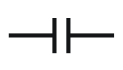
\includegraphics{capacitorSymbol}}

\device
\begin{alltt}
C<device name> <(+) node> <(-) node> [model name] [value]
+ [device parameters]
\end{alltt}

\model
\begin{alltt}
.MODEL <model name> C [model parameters]
.MODEL <model name> CAP [model parameters]
\end{alltt}

\examples
\begin{alltt}
CM12 2 4 5.288e-13
CLOAD 1 0 4.540pF IC=1.5V
CFEEDBACK 2 0 CMOD 1.0pF
CAGED 2 3 4.0uF D=0.0233 AGE=86200
CSOLDEP 3 0 C=\{ca*(c0+c1*tanh((V(3,0)-v0)/v1))\}
CSOLDEPQ 3 0 Q=\{ca*(c1*v1*ln(cosh((v(3,0)-v0)/v1))+c0*v(3,0))\}
\end{alltt}

\parameters
\begin{Parameters}
\param{device name}
The name of the device.

\param{\vbox{\hbox{(+) node\hfil}\hbox{(-) node}}}
Polarity definition for a positive voltage across the capacitor. The first
node is defined as positive. Therefore, the voltage across the component is
the first node voltage minus the second node voltage.

\param{model name}
If \texttt{model name} is omitted, then \texttt{value} is the capacitance in
farads.  If [model name] is given then the value is determined from the model
parameters; see the capacitor value formula below.

\param{value}
Positional specification of device parameter C (capacitance).  Alternately,
this can be specified as a parameter, \texttt{C=<value>}, or in the (optional)
model.

\param{device parameters}
Parameters listed in Table~\ref{C_1_Device_Instance_Params} may be provided as
space separated \texttt{<parameter>=<value>} specifications as needed.  Any number
of parameters may be specified.

\param{model parameters}
Parameters listed in Table~\ref{C_1_Device_Model_Params} may be provided as
space separated \texttt{<parameter>=<value>} specifications as needed.  Any number
of parameters may be specified.

\end{Parameters}

\comments
Positive current flows through the capacitor from
the \texttt{(+)} node to the \texttt{(-)} node.  In general, capacitors should
have a positive capacitance value (\texttt{<value>} property). In all cases,
the capacitance must not be zero.  

However, cases exist when a negative capacitance value may be used. This occurs
most often in filter designs that analyze an RLC circuit equivalent to a real
circuit. When transforming from the real to the RLC equivalent, the result may
contain a negative capacitance value.

In a transient run, negative capacitance values may cause the simulation to
fail due to instabilities they cause in the time integration
algorithms.

The power stored or released from the capacitor is calculated 
with $I \cdot \Delta V$ where the voltage drop is calculated as $(V_+ - V_-)$ 
and positive current flows from $V_+$ to $V_-$.

For compatibility with PSpice, either \texttt{C} or \texttt{CAP} can be used in a
\texttt{.MODEL} statement for a capacitor. 

The Multiplicity Factor (M) can be used to specify multiple, identical capacitors
in parallel. The effective capacitance becomes C*M. The M value need not be an
integer. It can be any positive real number. M can not be used as a model
parameter.

\end{Device}

\paragraph{Device Parameters}

% This table was generated by Xyce:
%   Xyce -doc C 1
%
\index{capacitor!device instance parameters}
\begin{DeviceParamTableGenerated}{Capacitor Device Instance Parameters}{C_1_Device_Instance_Params}
AGE & Age of capacitor & hour & 0 \\ \hline
C & Capacitance & F & 1e-06 \\ \hline
D & Age degradation coefficient & -- & 0.0233 \\ \hline
IC & Initial voltage drop across device & V & 0 \\ \hline
L & Semiconductor capacitor width & m & 1 \\ \hline
M & Multiplicity Factor & -- & 1 \\ \hline
Q & Charge & C & 0 \\ \hline
TC1 & Linear Temperature Coefficient & $^\circ$C$^{-1}$ & 0 \\ \hline
TC2 & Quadratic Temperature Coefficient & $^\circ$C$^{-2}$ & 0 \\ \hline
TEMP & Device temperature & $^\circ$C & Ambient Temperature \\ \hline
W & Semiconductor capacitor length & m & 1e-06 \\ \hline
\end{DeviceParamTableGenerated}


In addition to the parameters shown in the table, the capacitor supports a
vector parameter for the temperature correction coefficients.
\texttt{TC1=<linear coefficient>} and \texttt{TC2=<quadratic coefficient>} may
therefore be specified compactly as \texttt{TC=<linear coefficient>,<quadratic
coefficient>}.

\paragraph{Model Parameters}

% This table was generated by Xyce:
%   Xyce -doc C 1
%
\index{capacitor!device model parameters}
\begin{DeviceParamTableGenerated}{Capacitor Device Model Parameters}{C_1_Device_Model_Params}
C & Capacitance multiplier & -- & 1 \\ \hline
CJ & Junction bottom capacitance & F/m$^{2}$ & 0 \\ \hline
CJSW & Junction sidewall capacitance & F/m & 0 \\ \hline
DEFW & Default device width & m & 1e-06 \\ \hline
NARROW & Narrowing due to side etching & m & 0 \\ \hline
TC1 & Linear temperature coefficient & $^\circ$C$^{-1}$ & 0 \\ \hline
TC2 & Quadratic temperature coefficient & $^\circ$C$^{-2}$ & 0 \\ \hline
TNOM & Nominal device temperature & $^\circ$C & Ambient Temperature \\ \hline
\end{DeviceParamTableGenerated}


\paragraph{Capacitor Equations}

\subparagraph{Capacitance Value Formula}
If \texttt{[model name]} is specified, then the capacitance is given by:

\[
 \mathbf{C} \cdot (1 + \mathbf{TC1} \cdot (T - T_0) +
\mathbf{TC2} \cdot (T - T_0)^2)
\]
where \texttt{C} is the base capacitance specified on the device line
and is normally positive (though it can be negative, but not zero).
$T_0$ is the nominal temperature (set using \textrmb{TNOM} option).

\subparagraph{Age-aware Formula}
If \textrmb{AGE} is given, then the capacitance is:
\[\mathbf{C}[1 - \mathbf{D} \log(\mathbf{AGE})]\]

\subparagraph{Semiconductor Formula}
If \texttt{[model name]} and \textrmb{L} and \textrmb{W} are given, then the capacitance is:
\[
\mathbf{CJ}(\mathbf{L} - \mathbf{NARROW})(\mathbf{W} - \mathbf{NARROW}) + 2
\cdot \mathbf{CJSW}(\mathbf{L} - \mathbf{W} + 2 \cdot \mathbf{NARROW})
\]

\subparagraph{Solution-Dependent Capacitor}
If the capacitance (\texttt{C}) is set equal to an expression then a
``solution-dependent'' capacitor is used, where the capacitance is
a function of other simulation variables.  The formulas for
temperature-dependence and age-dependence, given above, then use that
calculated \texttt{C} value.

If the parameter \texttt{Q} is set equal to an expression {\em
  instead} of specifying a capacitance, this expression is used to
evaluate the charge on the capacitor instead of computing it from
capacitance.  Temperature and age dependence are not computed in this
case, as these effects are applied by modifying the capacitance.

Both solution-dependent charge and capacitance formulations are
implemented to assure charge conservation.  The capacitor:
\begin{alltt}
  c\_mcap 1 2 q=\{ca*(c1*v1*ln(cosh((v(1,2)-v0)/v1))+c0*v(1,2))\}
\end{alltt}
is exactly equivalent to the capacitor
\begin{alltt}
  c\_mcap 1 2 c=\{ca*(c0+c1*tanh((V(1,2)-v0)/v1))\}
\end{alltt}
because the capacitance is the derivative of the charge with respect
to the voltage drop across the capacitor.  Similarly, both are
equivalent to the behavioral source:
\begin{alltt}
  BC 1 2 I={ddt(V(1,2))*(ca*(c0+c1*tanh((V(1,2)-v0)/v1)))}
\end{alltt}
because $I=dQ/dt=dQ/dV*dV/dt=C*dV/dt$.

The restrictions for this formulation are:
\begin{XyceItemize}
  \item The expression used for \texttt{C} or \texttt{Q} must only use
    solution variables, which are node voltages and also branch
    currents for source devices.  It may not use device lead currents,
    which are post-processed quantities that are not solution variables.
  \item The expression must not use time derivatives.
  \item Capacitance (\texttt{C}) and Charge (\texttt{Q}) are the only
    instance or model parameters that are allowed to be
    solution-dependent.
\end{XyceItemize}

\paragraph{Other Restrictions and Caveats}
A netlist parsing error will occur if:
\begin{XyceItemize}
  \item Neither the \texttt{C}, \texttt{Q}, nor \texttt{L} instance
    parameters are specified.
  \item Both \texttt{C} and \texttt{Q} are specified as expressions.
    \item \texttt{Q} is specified in addition to an \texttt{IC=}.
  \item The \texttt{A} instance parameter is specified for a semiconductor 
      capacitor (which is specified via \texttt{L}, \texttt{W} and \texttt{CJSW}).
\end{XyceItemize}
If both the \texttt{C} and \texttt{L} instance parameters are specified then 
\texttt{C} will be used, rather than the semiconductor formulation. 

\paragraph{Special note on Initial Conditions:}

The IC parameter of the capacitor may be used to specify an initial
voltage drop on the capacitor.  Unlike SPICE3F5, this parameter is
never ignored (SPICE3F5 only respects it if UIC is used on a transient
line).  The initial condition is applied differently depending on the
analysis specified.

If one is doing a transient with DC operating point calculation or a
DC operating point analysis, the initial condition is applied by
inserting a voltage source across the capacitor to force the operating
point to find a solution with the capacitor charged to the specific
voltage.  The resulting operating point will be one that is consistent
with the capacitor having the given voltage in steady state.

If one specifies \texttt{UIC} or \texttt{NOOP} on the \texttt{.TRAN}
line, then \Xyce{} does not perform an operating point calculation,
but rather begins a transient simulation directly given an initial
state for the solution.  In this case, \texttt{IC} initial conditions
are applied only for the first iteration of the Newton solve of the
first time step --- the capacitor uses the initial condition to
compute its charge, and the nonlinear solver will therefore find a
solution to the circuit problem consistent with this charge, i.e., one
with the correct voltage drop across the capacitor.

The caveats of this section apply only to initial conditions specified
via \texttt{IC=} parameters on the capacitor, and do not affect how
initial conditions are applied when using \texttt{.IC} lines to
specify initial conditions on node values.

The three different ways of specifying initial conditions can lead to
different circuit behaviors.  Notably, when applying initial
conditions during a DC operating point with \texttt{IC=} on the
capacitor line, the resulting operating point will be a DC solution
with currents everywhere consistent with there being a constant charge
on the capacitor, whereas in general a transient run from an initial
condition {\em without\/} having performed an operating point
calculation will have a quiescent circuit at the first timestep.


%%
%% Inductor
%%
\clearpage
\subsection{Inductor}
\index{device!inductor} \index{inductor}
% Sandia National Laboratories is a multimission laboratory managed and
% operated by National Technology & Engineering Solutions of Sandia, LLC, a
% wholly owned subsidiary of Honeywell International Inc., for the U.S.
% Department of Energy’s National Nuclear Security Administration under
% contract DE-NA0003525.

% Copyright 2002-2021 National Technology & Engineering Solutions of Sandia,
% LLC (NTESS).


\begin{Device}\label{L_DEVICE}

\symbol
{
\includegraphics{inductorSymbol}}

\device
L<name> <(+) node> <(-) node> [model] <value> [device parameters]

\model
\begin{alltt}
.MODEL <model name> L [model parameters]
.MODEL <model name> IND [model parameters]
\end{alltt}

\examples
\begin{alltt}
L1 1 5 3.718e-08
LM 7 8 L=5e-3 M=2
LLOAD 3 6 4.540mH IC=2mA
Lmodded 3 6 indmod 4.540mH
.model indmod L (L=.5 TC1=0.010 TC2=0.0094)
\end{alltt}

\parameters

\begin{Parameters}
\param{\vbox{\hbox{(+) node\hfil}\hbox{(-) node}}}

Polarity definition for a positive voltage across the inductor. The
first node is defined as positive. Therefore, the voltage across the
component is the first node voltage minus the second node voltage.

\param{initial value}

The initial current through the inductor during the bias point
calculation.

\end{Parameters}

\comments
In general, inductors should have a positive
inductance value. The inductance must
not be zero.  Also, a netlist parsing error will occur if no value 
is specified for the inductance. 

However, cases exist when a negative value may be used.  This occurs most often
in filter designs that analyze an RLC circuit equivalent to a real circuit.
When transforming from the real to the RLC equivalent, the result may contain a
negative inductance value.

The power stored or released from the inductor is calculated 
with $I \cdot \Delta V$ where the voltage drop is calculated as $(V_+ - V_-)$ 
and positive current flows from $V_+$ to $V_-$.

If a model name is given, the inductance is modified from the value
given on the instance line by the parameters in the model card.  See
``Inductance Value Formula'' below.

When an inductor is named in the list of coupled inductors in a mutual
inductor device line (see page~\pageref{MutualInductor}) , and that
mutual inductor is of the nonlinear-core type, the \verb+<value>+ is
interpreted as a number of turns rather than as an inductance in
Henries.

For compatibility with PSpice, either \texttt{L} or \texttt{IND} can be used in a
\texttt{.MODEL} statement for an inductor. 

The Multiplicity Factor (\texttt{M}) can be used to specify multiple, identical 
inductors in parallel. The effective inductance becomes \texttt{L}/\texttt{M}.
However, the value for the \texttt{IC} instance parameter is not multiplied by 
the \texttt{M} value. The \texttt{M} value need not be an integer.  It can be 
any positive real number. \texttt{M} can not be used as a model parameter.

\end{Device}

\newpage
%\pagebreak

\paragraph{Device Parameters}
% This table was generated by Xyce:
%   Xyce -doc L 1
%
\index{inductor!device instance parameters}
\begin{DeviceParamTableGenerated}{Inductor Device Instance Parameters}{L_1_Device_Instance_Params}
IC & Initial current through device & A & 0 \\ \hline
L & Inductance & henry & 0 \\ \hline
M & Multiplicity Factor & -- & 1 \\ \hline
TC1 & Linear Temperature Coefficient & $^\circ$C$^{-1}$ & 0 \\ \hline
TC2 & Quadratic Temperature Coefficient & $^\circ$C$^{-2}$ & 0 \\ \hline
TEMP & Device temperature & $^\circ$C & Ambient Temperature \\ \hline
\end{DeviceParamTableGenerated}


\paragraph{Model Parameters}
% This table was generated by Xyce:
%   Xyce -doc L 1
%
\index{inductor!device model parameters}
\begin{DeviceParamTableGenerated}{Inductor Device Model Parameters}{L_1_Device_Model_Params}
IC & Initial current through device & A & 0 \\ \hline
L & Inductance Multiplier & -- & 1 \\ \hline
TC1 & First order temperature coeff. & $^\circ$C$^{-1}$ & 0 \\ \hline
TC2 & Second order temperature coeff. & $^\circ$C$^{-2}$ & 0 \\ \hline
TNOM & Reference temperature & $^\circ$C & 27 \\ \hline
\end{DeviceParamTableGenerated}


In addition to the parameters shown in the table, the inductor supports a vector parameter for the temperature correction coefficients.  \texttt{TC1=<linear coefficient>} and \texttt{TC2=<quadratic coefficient>} may therefore be specified compactly as \texttt{TC=<linear coefficient>,<quadratic coefficient>}.

\paragraph{Inductor Equations}

\subparagraph{Inductance Value Formula}
If \verb+[model name]+ is specified, then the inductance is given by:
\[\mathbf{L}_{base} \cdot \mathbf{L} \cdot (1 + \mathbf{TC1} \cdot (T - T_{0}) +
\mathbf{TC2} \cdot (T - T_{0})^{2})\]
where \texttt{$\mathbf{L}_{base}$} is the base inductance specified on the device line and is normally positive (though it can be
negative, but not zero).  $\mathbf{L}$ is the inductance multiplier specified in the model card.  $T_0$ is the nominal temperature (set using
\textrmb{TNOM} option).

%\subparagraph{Inductor Noise Equation}
%There is no noise model for the inductor.


%%
%% Mutual Inductors
%%
\clearpage
\subsection{Mutual Inductors}
\label{MutualInductor}
\index{device!mutualinductor} \index{mutualinductor}
% Sandia National Laboratories is a multimission laboratory managed and
% operated by National Technology & Engineering Solutions of Sandia, LLC, a
% wholly owned subsidiary of Honeywell International Inc., for the U.S.
% Department of Energy’s National Nuclear Security Administration under
% contract DE-NA0003525.

% Copyright 2002-2021 National Technology & Engineering Solutions of Sandia,
% LLC (NTESS).



\begin{Device}\label{K_DEVICE}

\symbol
{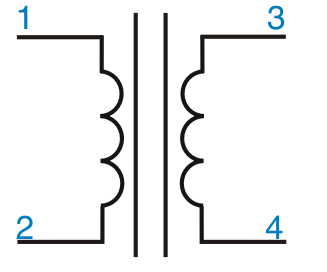
\includegraphics{transformerSymbol}}

\device
\begin{alltt}
K<name> L<inductor name> [L<inductor name>*]
+ <coupling value> [model name]
\end{alltt}

\model
.MODEL <model name> CORE [model parameters]

\examples
\begin{alltt}
ktran1 l1 l2 l3 1.0
KTUNED L3OUT  L4IN .8
KTRNSFRM LPRIMARY LSECNDRY 1
KXFRM L1 L2  L3  L4 .98 KPOT\_3C8
\end{alltt}

\parameters
\begin{Parameters}

\param{inductor name}

Identifies the inductors to be coupled. The inductors are coupled and in
the dot notation the dot is placed on the first node of each
inductor. The polarity is determined by the order of the nodes in the L
devices and not by the order of the inductors in the K statement.

If more than two inductors are given on a single K line, each inductor
is coupled to all of the others using the same coupling value.

\param{coupling value}

The coefficient of mutual coupling, which must be between $-1.0$ and
$1.0$.

This coefficient is defined by the equation
\begin{quote}
  \texttt{<coupling value>} = $\frac{M_{ij}}{\sqrt{L_iL_j}}$
\end {quote}

where
\begin{quote}
  $L_i$ is the inductance of the $i$th named inductor in the K-line
\end {quote}
\begin{quote}
    $M_{ij}$ is the mutual inductance between $L_i$ and $L_j$
\end {quote}
For transformers of normal geometry, use $1.0$ as the value. Values less
than $1.0$ occur in air core transformers when the coils do not
completely overlap.

\param{model name}

If \texttt{model name} is present, four things change:
\begin{itemize}
  \item The mutual coupling inductor becomes a nonlinear, magnetic core device.
  \item The inductors become windings, so the number specifying inductance now
        specifies the number of turns.
  \item The list of coupled inductors could be just one inductor.
  \item If two or more inductors are listed, each inductor is coupled to all others through the magnetic core.
  \item A model statement is required to specify the model parameters.
\end{itemize}

\end{Parameters}

\comments
Lead currents and power calculations are supported for the component inductors in both
linear and nonlinear mutual inductors.  They are not supported for the composite
mutual inductor though.  So, if \texttt{L1} is a component inductor for mutual inductor
\texttt{K1}, then requests for \texttt{I(L1)}, \texttt{P(L1)} and \texttt{W(L1)} will 
return lead current and power values as defined in Section~\ref{L_DEVICE}.  However, 
any usage of \texttt{I(K1)}, \texttt{P(K1)} and \texttt{W(K1)} will result in a 
\Xyce{} netlist parsing error.

\end{Device}

\paragraph{Model Parameters}
% This table was generated by Xyce:
%   Xyce -doc Min 1
%
\index{nonlinear mutual inductor!device model parameters}
\begin{DeviceParamTableGenerated}{Nonlinear Mutual Inductor Device Model Parameters}{Min_1_Device_Model_Params}
A & Thermal energy parameter & A/m & 1000 \\ \hline
ALPHA & Domain coupling parameter & -- & 5e-05 \\ \hline
AREA & Mean magnetic cross-sectional area & cm$^{2}$ & 0.1 \\ \hline
BETAH & Modeling constant & -- & 0.0001 \\ \hline
BETAM & Modeling constant & -- & 3.125e-05 \\ \hline
BHSIUNITS & Flag to report B and H in SI units & -- & 0 \\ \hline
C & Domain flexing parameter & -- & 0.2 \\ \hline
CLIM & Value below which domain flexing parameter will be treated as zero. & -- & 0.005 \\ \hline
CONSTDELVSCALING & Use constant scaling factor to smooth voltage difference over first inductor & V & false \\ \hline
DELVSCALING & Smoothing coefficient for voltage difference over first inductor & V & 1000 \\ \hline
FACTORMS & Flag to save state variables & -- & 0 \\ \hline
GAP & Effective air gap & cm & 0 \\ \hline
INCLUDEMEQU & Flag to include the magnetics in the solution. & -- & true \\ \hline
K & Domain anisotropy parameter & A/m & 500 \\ \hline
KIRR & Domain anisotropy parameter & A/m & 500 \\ \hline
LEVEL & for pspice compatibility -- ignored & -- & 0 \\ \hline
MEQNSCALING & M-equation scaling & -- & 1 \\ \hline
MS & Saturation magnetization & A/m & 1e+06 \\ \hline
MVARSCALING & M-variable scaling. & -- & 1 \\ \hline
OUTPUTSTATEVARS & Flag to save state variables & -- & 0 \\ \hline
PACK & for pspice compatibility -- ignored & -- & 0 \\ \hline
PATH & Total mean magnetic path & cm & 1 \\ \hline
PZEROTOL & Tolerance for nonlinear zero crossing & -- & 0.1 \\ \hline
REQNSCALING & R-equation scaling & -- & 1 \\ \hline
RVARSCALING & R-variable scaling & -- & 1 \\ \hline
TC1 & First order temperature coeff. & -- & 0 \\ \hline
TC2 & Second order temperature coeff. & -- & 0 \\ \hline
TNOM & Reference temperature & $^\circ$C & 27 \\ \hline
\end{DeviceParamTableGenerated}


Note that \Xyce's default value for the $\mbox{GAP}$ parameter as zero.  Some simulators
will use non-zero values of the $\mbox{GAP}$ as a default.  When using netlists from 
other simulators in \Xyce, ensure that the default parameters are consistent. 

\subparagraph{Special Notes}

The coupling coefficient of the linear mutual
inductor (i.e. a mutual inductor without a core model) is permitted to
be a time- or solution variable-dependent expression.  This is
intended to allow simulation of electromechnical devices in which
there might be moving coils that interact with fixed coils.  

Additionally, for linear mutual inductors,
different coupling terms can be applied to different pairs of inductors with this syntax:
{\tt 
\begin{verbatim}
L1 1 2 2.0e-3
L2 0 3 8.1e-3
L3 3 4 8.1e-3 
ktran1 l1 l2 0.7
ktran2 l2 l3 0.9
ktran3 l1 l3 0.99
\end{verbatim}
}

Nonlinear mutual inductors can output $B(t)$ and $H(t)$ variables so that
one can plot $B-H$ loops.  On the {\tt .print} line the $B$ and $H$ variables 
are accessible using the node output syntax as in {\tt n( non-linear-inductor-name\_b )} for $B$
and {\tt n( non-linear-inductor-name\_h )} for $H$.  A confusing aspect of this is that 
the non-linear inductor name is the {\em internal } name used by \Xyce{}.  For example, 
consider this circuit which defines a nonlinear mutual inductor at both the top level of
the circuit and within a subcircuit:

{\tt 
\begin{verbatim}
* Test Circuit for Mutually Coupled Inductors

VS 0 1 SIN(0 169.7 60HZ)
R1 1 2 1K
R2 3 0 1K
L1 2 0 10
L2 3 0 20
K1 L1 L2 0.75 txmod
.model txmod core 

.subckt mysub n1 n2 n3 
r1s n1 n2 1000
r2s n3 0  1000
L1s n2 0  10
L2s n3 0  20   
k1s L1s L2s 0.75 txmod
.ends

xtxs 1 4 5 mysub

.TRAN 100US 25MS

* output the current through each inductor and the B & H values.
.PRINT TRAN I(L1) I(L2) n(ymin!k1_b)  n(ymin!k1_h)  
+ I(xtxs:L1s)  I(xtxs:l2s) n(xtxs:ymin!k1s_b) n(xtxs:ymin!k1s_h)

.END
\end{verbatim}
}

The internal, \Xyce{} name of the non-linear mutual inductor is {\tt
YMIN!K1} or {\tt ymin!k1} as the name is not
case-sensitive.  The device {\tt k1s} is declared within a
subcircuit called {\tt xtxs}. Thus, its full name is {\tt
xtxs:ymin!k1s}. The reason for this is that both the linear and
non-linear mutual inductors are devices that are collections of other
devices, inductors in this case.  Rather than use one of the few
remaining single characters left to signify a new device, \Xyce{} uses
{\tt Y} devices as an indicator of a extended device set, where the
characters after the {\tt Y} denote the device type and then the device
name.  Here, {\tt ymin } means a {\tt min } device which is a {\em
mutual-inductor, non-linear} device.  Thus, to print the $B$ or $H$
variable of the non-linear mutual inductor called {\tt k1} one would
use {\tt n(ymin!k1\_b)} and {\tt n(ymin!k1\_h)}
respectively for a {\tt .print} line that looks like this:

{\tt 
\begin{verbatim}
.PRINT TRAN I(L1) I(L2) n(ymin!k1_b)  n(ymin!k1_h)  
\end{verbatim}
}

And if the mutual inductor is in a subcircuit called {\tt xtxs} then the 
{\tt .print} line would look like this:

{\tt 
\begin{verbatim}
.PRINT TRAN I(xtxs:L1s)  I(xtxs:l2s) n(xtxs:ymin!k1s_b) n(xtxs:ymin!k1s_h)
\end{verbatim}
}

The above example also demonstrates how one outputs the current through inductors 
that are part of mutual inductors.  
The syntax is {\tt I( inductor name )}.

Note that while MKS units are used internally in \Xyce{}, $B$ and $H$ are output
by default in the SI units of Gauss for $B$ and Oersted for $H$.
To convert $B$ to units of Tesla divide  \Xyce{}'s output by $10,000$.  
To convert $H$ to units of $A/m$ divide  \Xyce{}'s output by $4\pi/1000$. 
Additionally, one can set the {\tt .model CORE }
parameter {\tt BHSIUNITS } to 1 to force $B$ and $H$ to be output in MKS
units. 


Finally, one can access the $B$ and $H$ data via the {\tt .model
CORE} line. On the nonlinear mutual inductor's {\tt .model} line, set the
option {\tt OUTPUTSTATEVARS=1}. This will cause \Xyce{} to create a unique
file for each nonlinear mutual inductor that uses this {\tt .model} line
with a name of the form {\tt Inductor\_}device\_name.  There are five
columns of data in this file: time ($t$), magnetic moment ($M$), total
current flux ($R$), flux density ($B$) and magnetic field strength
($H$).  As with data output on the {\tt .print} line, SI units are used
such that $B$ is output with units of Gauss and $H$ in Oersted.  As
mentioned earlier, setting the model flag {\tt BHSIUNITS } to 1 causes
the output of $B$ and $H$ uses MKS units of Tesla and $A/m$
respectively. 

\index{mutualinductor!mutual inductor equations}
\subparagraph{Mutual Inductor Equations}

The voltage to current relationship for a set of linearly coupled inductors is:
\begin{equation}
V_{i} = \sum_{j=1}^{N} c_{ij} \sqrt{ L_{i} L_{j} } \frac{dI_{j}}{dt}
\label{linMIRelation}
\end{equation}

Here, $V_{i}$ is the voltage drop across the $i$th inductor in the coupled set.
The coupling coefficient between a pair of inductors is $c_{ij}$ with a value typically
near unity and $L$ is the inductance of a given inductor which has units of
\emph{Henry's} (1 Henry $ = 1 H = Volt \cdot s / Amp $)

For nonlinearly coupled inductors, the above equation is expanded to the form:
\begin{equation}
V_{i} = \left[1 + \left(1-\frac{\ell_g}{\ell_t}\right)P(M,I_{1} ... I_{N})\right]\sum_{j=1}^{N} Lo_{ij} \frac{dI_{j}}{dt}
\label{nonlinMIRelation}
\end{equation}
This is similar in form to the linearly coupled inductor equation.  However,
the coupling has become more complicated as it now depends on the magnetic moment
created by the current flow, $M$.  Additionally, there are geometric factors,
$\ell_{g}$ and $\ell_{t}$ which are the effective air gap and total mean magnetic
path for the coupled inductors. The matrix of terms, $Lo_{ij}$ is defined as
\begin{equation}
Lo_{ij}=\frac{\mu_0 A_c N_i N_j}{\ell_t}
\end{equation}
and it represents the physical coupling between inductors $i$ and $j$.  In this
expression, $N_i$ is the number of windings around the core of inductor $i$,
$\mu_0$ is the magnetic permeability of free space which has units of Henries per meter
and a value of $4\pi \times 10^{-7}$ and $A_c$ is the mean magnetic cross-sectional area.

The magnetic moment, $M$ is defined by:
\begin{equation}
\frac{dM}{dt} = \frac{1}{\ell_t} P \sum_{i=1}^{N} N_i \frac{dI_i}{dt}
\end{equation}
and the function $P$ is defined as:
\begin{equation}
P = \frac{c M'_{an} + (1-c)M'_{irr}}{1 + \left(\frac{\ell_g}{\ell_t}-\alpha\right) c M'_{an} + \frac{\ell_g}{\ell_t}(1-c)M'_{irr}}
\end{equation}
If $c < \mbox{CLIM}$, then $c$ is treated as zero in the above equation and \Xyce\/ 
simplifies the formulation.  In this case, the magnetic-moment equation will not be 
needed and it will be be dropped form the formulation.  One can controll this behavior by
modifying the value of $\mbox{CLIM}$.

The remaining functions are:
\begin{eqnarray}
M'_{an} & = & \frac{M_s A}{\left(A + |H_e|\right)^2} \\
H_e & = & H + \alpha M \\
H & = & H_{app} - \frac{\ell_g}{\ell_t}M  \\
H_{app} & = & \frac{1}{\ell_t}\sum_{i=1}^{N} N_i I_i \\
M'_{irr} & = & \frac{\Delta M sgn(q) + |\Delta M|}{2\left(K_{irr} - \alpha |\Delta  M|\right)} \\
\Delta M & = & M_{an} - M \\
M_{an} & = & \frac{M_s H_e}{A + |H_e|} \\
q & = & \mbox{DELVSCALING}  \Delta V
\end{eqnarray}

\Xyce\/ dynamically modifies $\mbox{DELVSCALING}$ to be $1000 / $ Maximum Voltage Drop over the 
first inductor.  This typically produces accurate results for both low voltage and high 
voltage applicaitons.  However, it is possible to use a fixed scaling by setting the 
model parameter $\mbox{CONSTDELVSCALING}$ to true and then setting $\mbox{DELVSCALING}$ 
to the desired scaling value.

In \Xyce{}'s formulation, we define $R$ as:
\begin{equation}
R = \frac{dH_{app}}{dt} = \frac{1}{\ell_t}\sum_{i=1}^{N} N_i \frac{dI_i}{dt}
\end{equation}
This simplifies the $M$ equation to:
\begin{equation}
\frac{dM}{dt} =  P R
\end{equation}
\Xyce{} then solves for the additional variables $M$ and $R$ when modeling a nonlinear
mutual inductor device.

\subparagraph{B-H Loop Calculations}
\index{mutualinductor!B-H loop calculations}
To calculate $B$-$H$ loops, $H$ is used as defined above and $B$ is a derived quantity
calculated by:
\begin{eqnarray}
B & = & \mu_0 \left( H + M \right) \\
  & = & \mu_0 \left[ H_{app} + \left(1 - \frac{\ell_g}{\ell_t}\right) M \right]
\end{eqnarray}

\subparagraph{Converting Nonlinear to Linear Inductor Models} 
\index{mutualinductor!Converting nonlinear to linear mutual indcutors}
At times one may have a model for nonlinear mutual inductor, but wish to use a 
simpler linear model in a given circuit.  To convert a non-linear model to an 
equivalent linear form, one can start by equating the coupling components of 
equations~\ref{linMIRelation} and~\ref{nonlinMIRelation} as:

\begin{equation}
 c_{ij} \sqrt{ L_{i} L_{j} } =  \left[1 + \left(1-\frac{\ell_g}{\ell_t}\right)P(M,I_{1} ... I_{N})\right] Lo_{ij}
\label{nonlinMIRelation2}
\end{equation}
In the above relationship, $i$ and $j$ represent the $i$th and $j$th inductors.  Since we would like to 
equate the $i$th inductor's nonliner properties to its linear properties, we will substitute $i\rightarrow j$ 
and simplify assuming steady state where $d/dt = 0$ and $M(t) = 0$.

\begin{equation}
L_{i} = \frac{1}{c_{ii}} \left\{ 1 + \left(1 - \frac{\ell_g}{\ell_t}  \right) 
  \left[\frac{c \frac{Ms}{A}}{1 + \left( \frac{\ell_g}{\ell_t} - \alpha\right) \frac{Ms}{A}} \right] \right\} \frac{\mu A_c}{\ell_t} N_i^2
  \label{inductanceFromWindings}
\end{equation}

In the above equatin, $c_{ii}$ represents the coupling coefficient between the $i$th inductor with itself.  
This will likely be $1$ unless there are very unusual geometry considerations.  Note, that the terms $A$, $Ms$, $A_c$, $\mu$,
$\ell_{g}$ and $\ell_{t}$ all have units of length within them and must use the same unit for this relationship 
to be valid.  Specifically, $\mu$ has units of Henery's per meter and $A$ and $Ms$ have units of Amps per meter.   
$A_c$, $\ell_{g}$ and $\ell_{p}$ have units of length$^2$ and length respectively, but the length unit used in 
the model statement is $cm^2$ and $cm$ respectively.  Thus, one must use consistent units such as meters 
for $A_c$, $\ell_{g}$ and $\ell_{p}$ in equation~\ref{inductanceFromWindings} for a valid inductance approximation.



%%
%% Resistor
%%
\clearpage
\subsection{Resistor}
\index{device!resistor} \index{resistor}
% Sandia National Laboratories is a multimission laboratory managed and
% operated by National Technology & Engineering Solutions of Sandia, LLC, a
% wholly owned subsidiary of Honeywell International Inc., for the U.S.
% Department of Energy’s National Nuclear Security Administration under
% contract DE-NA0003525.

% Copyright 2002-2020 National Technology & Engineering Solutions of Sandia,
% LLC (NTESS).


\begin{Device}

\symbol
{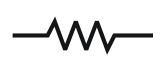
\includegraphics{resistorSymbol}}

\device
R<name> <(+) node> <(-) node> [model name] [value] [device parameters]

\model
\begin{alltt}
.MODEL <model name> R [model parameters]
.MODEL <model name> RES [model parameters]
\end{alltt}

\examples
\begin{alltt}
R1 1 2 2K TEMP=27
RM 4 5 R=4e3 M=2
RLOAD 3 6 RTCMOD 4.540 TEMP=85
.MODEL RTCMOD R (TC1=.01 TC2=-.001)
RSEMICOND 2 0 RMOD L=1000u W=1u
.MODEL RMOD R (RSH=1)
\end{alltt}

\parameters

\begin{Parameters}

\param{\vbox{\hbox{(+) node\hfil}\hbox{(-) node}}}

Polarity definition for a positive voltage across the resistor. The
first node is defined as positive. Therefore, the voltage across the
component is the first node voltage minus the second node voltage.
Positive current flows from the positive node (first node) to the
negative node (second node).

\param{model name}

If \texttt{[model name]} is omitted, then \texttt{[value]} is the
resistance in Ohms. If \texttt{[model name]} is given then the
resistance is determined from the model parameters; see the resistance
value formula below.

\param{value}

Positional specification of device parameter R (resistance).
Alternately, this can be specified as a parameter, \texttt{R=<value>},
or in the (optional) model.

\param{device parameters}

Parameters listed in Table~\ref{R_1_Device_Instance_Params} may be provided as
space separated \texttt{<parameter>=<value>} specifications as needed.
Any number of parameters may be specified.

\end{Parameters}

\comments

Resistors can have either positive or negative resistance values (R).  A zero 
resistance value (R) is also allowed. 

The power dissipated in the resistor is calculated 
with $I \cdot \Delta V$ where the voltage drop is calculated as $(V_+ - V_-)$ 
and positive current flows from $V_+$ to $V_-$.  The power accessors
(\texttt{P()} and \texttt{W()}) are supported for both the level 1 resistor
and the level 2 (thermal) resistor.

For compatibility with PSpice, either \texttt{R} or \texttt{RES} can be used in a
\texttt{.MODEL} statement for a resistor.

The Multiplicity Factor (\texttt{M}) can be used to specify multiple, identical 
resistors in parallel. The effective resistance becomes \texttt{R}/\texttt{M}.  
The \texttt{M} value need not be an integer.  It can be any positive real number.  
\texttt{M} can not be used as a model parameter. 

\end{Device}

\newpage
%\pagebreak

\paragraph{Device Parameters}
% This table was generated by Xyce:
%   Xyce -doc R 1
%
\index{resistor!device instance parameters}
\begin{DeviceParamTableGenerated}{Resistor Device Instance Parameters}{R_1_Device_Instance_Params}
DTEMP & Device Temperature -- For compatibility only. Parameter is NOT used & $^\circ$C & 0 \\ \hline
L & Length & m & 0 \\ \hline
M & Multiplicity Factor & -- & 1 \\ \hline
R & Resistance & $\mathsf{\Omega}$ & 1000 \\ \hline
TC1 & Linear Temperature Coefficient & $^\circ$C$^{-1}$ & 0 \\ \hline
TC2 & Quadratic Temperature Coefficient & $^\circ$C$^{-2}$ & 0 \\ \hline
TCE & Exponential Temperature Coefficient & \%$/^\circ$C & 0 \\ \hline
TEMP & Device temperature & $^\circ$C & Ambient Temperature \\ \hline
W & Width & m & 0 \\ \hline
\end{DeviceParamTableGenerated}


In addition to the parameters shown in the table, the resistor supports a vector parameter for the temperature correction coefficients.  \texttt{TC1=<linear coefficient>} and \texttt{TC2=<quadratic coefficient>} may therefore be specified compactly as \texttt{TC=<linear coefficient>,<quadratic coefficient>}.

\paragraph{Model Parameters}
% This table was generated by Xyce:
%   Xyce -doc R 1
%
\index{resistor!device model parameters}
\begin{DeviceParamTableGenerated}{Resistor Device Model Parameters}{R_1_Device_Model_Params}
DEFW & Default Instance Width & m & 1e-05 \\ \hline
NARROW & Narrowing due to side etching & m & 0 \\ \hline
R & Resistance Multiplier & -- & 1 \\ \hline
RSH & Sheet Resistance & $\mathsf{\Omega}$ & 0 \\ \hline
TC1 & Linear Temperature Coefficient & $^\circ$C$^{-1}$ & 0 \\ \hline
TC2 & Quadratic Temperature Coefficient & $^\circ$C$^{-2}$ & 0 \\ \hline
TCE & Exponential Temperature Coefficient & \%$/^\circ$C & 0 \\ \hline
TNOM & Parameter Measurement Temperature & $^\circ$C & Ambient Temperature \\ \hline
\end{DeviceParamTableGenerated}


Note: There is no model parameter for Default Instance Length.  The use of the semiconductor resistor model requires
the user to specify a non-zero value for the instance parameter \texttt{L}. 

\paragraph{Resistor Equations}

\subparagraph{Resistance Value Formulas}
If the \textrmb{R} parameter is given on the device instance line 
then that value is used.

If the \textrmb{R} parameter is not given then the semiconductor resistor model
will be used if the \textrmb{L} instance parameter and the \textrmb{RSH} model parameter
are given and both are non-zero.  In that case the resistance will be as follows.
(Note: If \textrmb{W} is not given on the instance line then the value
for the model parameter \textrmb{DEFW} will be used instead.)

\[
\mathbf{RSH} \frac{[\mathbf{L} - \mathbf{NARROW}]}
{[\mathbf{W} - \mathbf{NARROW}]}
\]

If neither of these two cases apply then the default value for
the \textrmb{R} parameter will be used.     

\subparagraph{Temperature Dependence}
If \textrmb{TCE} is specified as either an instance or model parameter
for the Level 1 resistor then the resistance at temperature $T$
is given by (where the resistance at the nominal temperature ($T_{0}$) 
was defined above in the resistance value formulas):

\[
\mathbf{R} \cdot pow(1.01,\mathbf{TCE} \cdot (T - T_{0}))
\]

otherwise the resistance is given by:
\[
\mathbf{R} \cdot (1 + \mathbf{TC1} \cdot (T - T_{0}) + \mathbf{TC2}
\cdot (T - T_0)^2)
\]

\paragraph{Thermal (level=2) Resistor}

\Xyce{} supports a thermal resistor model, which is associated with level=2.

\paragraph{Thermal Resistor Instance Parameters}
% This table was generated by Xyce:
%   Xyce -doc R 2
%
\index{resistor!device instance parameters}
\begin{DeviceParamTableGenerated}{Resistor Device Instance Parameters}{R_2_Device_Instance_Params}
A & Area of conductor & m$^{2}$ & 0 \\ \hline
DENSITY & Resistor material density (unused) & kg/$\mbox{m}^3$ & 0 \\ \hline
HEATCAPACITY & Resistor material volumetric heat capacity & $J/(\mbox{m}^3{}$K) & 0 \\ \hline
L & Length of conductor & m & 0 \\ \hline
M & Multiplicity Factor & -- & 1 \\ \hline
OUTPUTINTVARS & Debug Output switch & -- & false \\ \hline
R & Resistance & $\mathsf{\Omega}$ & 1000 \\ \hline
RESISTIVITY & Resistor material resistivity & $\mathsf{\Omega}$ m & 0 \\ \hline
TEMP & Device temperature & $^\circ$C & Ambient Temperature \\ \hline
THERMAL\_\-A & Area of material thermally coupled to conductor & m$^{2}$ & 0 \\ \hline
THERMAL\_\-HEATCAPACITY & Volumetric heat capacity of material thermally coupled to conductor & $J/(\mbox{m}^3{}$K) & 0 \\ \hline
THERMAL\_\-L & Length of material thermally coupled to conductor & m & 0 \\ \hline
W & Width of conductor & m & 0 \\ \hline
\end{DeviceParamTableGenerated}



%%
%% Resistor Model Param Table
%%
\paragraph{Thermal Resistor Model Parameters}
% This table was generated by Xyce:
%   Xyce -doc R 2
%
\index{resistor!device model parameters}
\begin{DeviceParamTableGenerated}{Resistor Device Model Parameters}{R_2_Device_Model_Params}
DEFW & Default Instance Width & m & 1e-05 \\ \hline
DENSITY & Resistor material density (unused) & kg/$\mbox{m}^3$ & 0 \\ \hline
HEATCAPACITY & Resistor material volumetric heat capacity & $J/(\mbox{m}^3{}$K) & 0 \\ \hline
NARROW & Narrowing due to side etching & m & 0 \\ \hline
R & Resistance Multiplier & -- & 1 \\ \hline
RESISTIVITY & Resistor material resistivity & $\mathsf{\Omega}$ m & 0 \\ \hline
RSH & Sheet Resistance & $\mathsf{\Omega}$ & 0 \\ \hline
TC1 & Linear Temperature Coefficient & $^\circ$C$^{-1}$ & 0 \\ \hline
TC2 & Quadratic Temperature Coefficient & $^\circ$C$^{-2}$ & 0 \\ \hline
TCE & Exponential Temperature Coefficient & \%$/^\circ$C & 0 \\ \hline
THERMAL\_HEATCAPACITY & Volumetric heat capacity of material thermally coupled to conductor & $J/(\mbox{m}^3{}$K) & 0 \\ \hline
TNOM & Nominal device temperature & $^\circ$C & Ambient Temperature \\ \hline
\end{DeviceParamTableGenerated}


The temperature model for the thermal resistor will be enabled
if the \textrmb{A} and \textrmb{L} instance parameters are 
given and the parameters \textrmb{HEATCAPACITY} and
\textrmb{RESISTIVITY} are also given as a pair of either 
instance parameters or model parameters.  Otherwise, the
resistance value and temperature dependence of the Level 2
resistor will follow the equations for the Level 1 resistor 
given above, with the caveat that \texttt{TCE} is only 
allowed as a model parameter for the Level 2 resistor.

If the temperature model for the Level 2 resistor is enabled,
then the resistance ($R$) is given by the following, where the 
\textrmb{RESISTIVITY} can be a temperature-dependent expression:

\[
\frac{\mathbf{RESISTIVITY} \cdot \mathbf{L}}
{\mathbf{A}}
\]

The rate-of-change ($dT/dt$) of the temperature ($T$) of the 
thermal resistor with time is then given by the following where 
$i_{0}$ is the current through the resistor:

\[
\frac{i_{0} \cdot i_{0} \cdot R}
{(\mathbf{A} \cdot \mathbf{L} \cdot \mathbf{HEATCAPACITY}) +
 (\mathbf{THERMAL\_A} \cdot \mathbf{THERMAL\_L} \cdot \mathbf{THERMAL\_HEATCAPACITY})}
\]


%%
%% Diode
%%
\clearpage
\subsection{Diode}
\index{device!diode} \index{diode}
% Sandia National Laboratories is a multimission laboratory managed and
% operated by National Technology & Engineering Solutions of Sandia, LLC, a
% wholly owned subsidiary of Honeywell International Inc., for the U.S.
% Department of Energy’s National Nuclear Security Administration under
% contract DE-NA0003525.

% Copyright 2002-2020 National Technology & Engineering Solutions of Sandia,
% LLC (NTESS).


\begin{Device}\label{D_DEVICE}

\symbol
{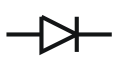
\includegraphics{diodeSymbol}}

\device
D<name> <(+) node> <(-) node> <model name> [area value]

\model
.MODEL <model name> D [model parameters]

\examples
\begin{alltt}
  DCLAMP 1 0 DMOD
  D2 15 17 SWITCH 1.5
\end{alltt}

\parameters
\begin{Parameters}

\param{\vbox{\hbox{(+) node\hfil}\hbox{(-) node}}}

The anode and the cathode.

\param{area value} 

Scales IS, ISR, IKF, RS, CJO, and IBV, and has a default value of 1.
IBV and BV are both specified as positive values.

\end{Parameters}

\comments

The diode is modeled as an ohmic resistance (\texttt{RS/area}) in series
with an intrinsic diode.  Positive current is current flowing from the
anode through the diode to the cathode. 

The power through the diode is calculated 
with $I \cdot \Delta V$ where the voltage drop is calculated as $(V_+ - V_-)$ 
and positive current flows from $V_+$ to $V_-$.  This formula may differ from
other simulators, such as HSPICE.

\end{Device}

\paragraph{Diode Operating Temperature}
\index{diode!operating temperature} Model parameters can be assigned unique
measurement temperatures using the \textrmb{TNOM} model parameter.

\paragraph{Diode level selection}

Three distinct implementations of the diode are available.  These are
selected by using the \verb|LEVEL| model parameter.  The default
implementation is based on SPICE 3F5, and may be explicitly specified
using \verb|LEVEL=1| in the model parameters, but is also selected if no
\verb|LEVEL| parameter is specified.  The PSpice implementation
~\cite{PSpiceUG:1998} is obtained by specifying \verb|LEVEL=2|.
The \Xyce{} \verb|LEVEL=200| diode is the JUNCAP200 model.

The \Xyce{} \verb|LEVEL=1| and \verb|LEVEL=2| diodes have a parameter,
\textrmb{IRF}, that allows the user to adjust the reverse current from
the basic SPICE implementation.  The usual SPICE treatment defines the
linear portion of the reverse current in terms of IS which is defined
by the forward current characteristics.  Data shows that often the
reverse current is quite far off when determined in this manner.  The
parameter \textrmb{IRF} is a multiplier that can be applied to adjust
the linear portion of the reverse current.  \textbf{NOTE: The
  adjustment applied when IRF is specified is not well validated and
  is known in some circumstances to cause non-physical solution
  discontinuities and/or simulation failure.  It is a deprecated
  feature as of \Xyce{} 6.11, and may be removed in a future release.
  If IRF is left unspecified, the diode reverts to being compatible
  with the SPICE3F5 diode model.  If IRF is specified in the model
  card, even if the default value of 1.0 is used in the specification,
  a temperature correction factor is applied that makes the device
  incompatible with SPICE3F5's model.  For this reason, any
  specification of IRF in the model card will result in a warning from
  versions of \Xyce{} after 6.11.}



\pagebreak

\paragraph{Level 1 and 2 Diode Instance Parameters}
% This table was generated by Xyce:
%   Xyce -doc D 1
%
\index{diode!device instance parameters}
\begin{DeviceParamTableGenerated}{Diode Device Instance Parameters}{D_1_Device_Instance_Params}
AREA & Area scaling value (scales IS, ISR, IKF, RS, CJ0, and IBV) & -- & 1 \\ \hline
IC &  & -- & 0 \\ \hline
LAMBERTW & Option to solve diode equations with the Lambert-W function & logical (T/F) & 0 \\ \hline
OFF & Initial voltage drop across device set to zero & logical (T/F) & 0 \\ \hline
TEMP & Device temperature & -- & Ambient Temperature \\ \hline
\end{DeviceParamTableGenerated}


\paragraph{Level 1 and 2 Diode Model Parameters}
% This table was generated by Xyce:
%   Xyce -doc D 1
%
\index{diode!device model parameters}
\begin{DeviceParamTableGenerated}{Diode Device Model Parameters}{D_1_Device_Model_Params}
AF & Flicker noise exponent & -- & 1 \\ \hline
BV & Reverse breakdown "knee" voltage & V & 1e+99 \\ \hline
CJ & Zero-bias p-n depletion capacitance & F & 0 \\ \hline
CJ0 & Zero-bias p-n depletion capacitance & F & 0 \\ \hline
CJO & Zero-bias p-n depletion capacitance & F & 0 \\ \hline
EG & Bandgap voltage (barrier height) & eV & 1.11 \\ \hline
FC & Forward-bias depletion capacitance coefficient & -- & 0.5 \\ \hline
IBV & Reverse breakdown "knee" current & A & 0.001 \\ \hline
IBVL & Low-level reverse breakdown "knee" current (level 2) & A & 0 \\ \hline
IKF & High-injection "knee" current (level 2) & A & 0 \\ \hline
IRF & Reverse current fitting factor & -- & 1 \\ \hline
IS & Saturation current & A & 1e-14 \\ \hline
ISR & Recombination current parameter (level 2) & A & 0 \\ \hline
JS & Saturation current & A & 1e-14 \\ \hline
KF & Flicker noise coefficient & -- & 0 \\ \hline
M & Grading parameter for p-n junction & -- & 0.5 \\ \hline
N & Emission coefficient & -- & 1 \\ \hline
NBV & Reverse breakdown ideality factor (level 2) & -- & 1 \\ \hline
NBVL & Low-level reverse breakdown ideality factor (level 2) & -- & 1 \\ \hline
NR & Emission coefficient for ISR (level 2) & -- & 2 \\ \hline
RS & Parasitic resistance & $\mathsf{\Omega}$ & 0 \\ \hline
TBV1 & BV temperature coefficient (linear) (level 2) & $^\circ$C$^{-1}$ & 0 \\ \hline
TBV2 & BV temperature coefficient (quadratic) (level 2) & $^\circ$C$^{-2}$ & 0 \\ \hline
TIKF & IKF temperature coefficient (linear) (level 2) & $^\circ$C$^{-1}$ & 0 \\ \hline
TNOM &  & -- & Ambient Temperature \\ \hline
TRS1 & RS temperature coefficient (linear) (level 2) & $^\circ$C$^{-1}$ & 0 \\ \hline
TRS2 & RS temperature coefficient (quadratic) (level 2) & $^\circ$C$^{-2}$ & 0 \\ \hline
TT & Transit time & s & 0 \\ \hline
VB & Reverse breakdown "knee" voltage & V & 1e+99 \\ \hline
VJ & Potential for p-n junction & V & 1 \\ \hline
XTI & IS temperature exponent & -- & 3 \\ \hline
\end{DeviceParamTableGenerated}


The JUNCAP200 model has the instance and model parameters in the
tables below.  Complete documentation of JUNCAP200 may be found at
\url{http://www.cea.fr/cea-tech/leti/pspsupport/Documents/juncap200p5_summary.pdf}.

\paragraph{JUNCAP200 Instance Parameters}
% This table was generated by Xyce:
%   Xyce -doc D 200
%
\index{juncap200 diode!device instance parameters}
\begin{DeviceParamTableGenerated}{JUNCAP200 Diode Device Instance Parameters}{D_200_Device_Instance_Params}
AB & Junction area & m$^{2}$ & 1e-12 \\ \hline
LG & Gate-edge part of junction perimeter & m$^{2}$ & 1e-06 \\ \hline
LS & STI-edge part of junction perimeter & m$^{2}$ & 1e-06 \\ \hline
M &  Alias for MULT & --- & 1 \\ \hline
MULT & Number of devices in parallel & --- & 1 \\ \hline
\end{DeviceParamTableGenerated}


\paragraph{JUNCAP200 Model Parameters}
% This table was generated by Xyce:
%   Xyce -doc D 200
%
\index{juncap200 diode!device model parameters}
\begin{DeviceParamTableGenerated}{JUNCAP200 Diode Device Model Parameters}{D_200_Device_Model_Params}
CBBTBOT & Band-to-band tunneling prefactor of bottom component & A/V$^{3}$ & 1e-12 \\ \hline
CBBTGAT & Band-to-band tunneling prefactor of gate-edge component & Am/V$^{3}$ & 1e-18 \\ \hline
CBBTSTI & Band-to-band tunneling prefactor of STI-edge component & Am/V$^{3}$ & 1e-18 \\ \hline
CJORBOT & Zero-bias capacitance per unit-of-area of bottom component & F/m$^{2}$ & 0.001 \\ \hline
CJORGAT & Zero-bias capacitance per unit-of-length of gate-edge component & F/m & 1e-09 \\ \hline
CJORSTI & Zero-bias capacitance per unit-of-length of STI-edge component & F/m & 1e-09 \\ \hline
CSRHBOT & Shockley-Read-Hall prefactor of bottom component & A/m$^{3}$ & 100 \\ \hline
CSRHGAT & Shockley-Read-Hall prefactor of gate-edge component & A/m$^{2}$ & 0.0001 \\ \hline
CSRHSTI & Shockley-Read-Hall prefactor of STI-edge component & A/m$^{2}$ & 0.0001 \\ \hline
CTATBOT & Trap-assisted tunneling prefactor of bottom component & A/m$^{3}$ & 100 \\ \hline
CTATGAT & Trap-assisted tunneling prefactor of gate-edge component & A/m$^{2}$ & 0.0001 \\ \hline
CTATSTI & Trap-assisted tunneling prefactor of STI-edge component & A/m$^{2}$ & 0.0001 \\ \hline
DTA & Temperature offset with respect to ambient temperature & K & 0 \\ \hline
FBBTRBOT & Normalization field at the reference temperature for band-to-band tunneling of bottom component & Vm$^{-1}$ & 1e+09 \\ \hline
FBBTRGAT & Normalization field at the reference temperature for band-to-band tunneling of gate-edge component & Vm$^{-1}$ & 1e+09 \\ \hline
FBBTRSTI & Normalization field at the reference temperature for band-to-band tunneling of STI-edge component & Vm$^{-1}$ & 1e+09 \\ \hline
FJUNQ & Fraction below which junction capacitance components are considered negligible & --- & 0.03 \\ \hline
FREV & Coefficient for reverse breakdown current limitation & --- & 1000 \\ \hline
IDSATRBOT & Saturation current density at the reference temperature of bottom component & A/m$^{2}$ & 1e-12 \\ \hline
IDSATRGAT & Saturation current density at the reference temperature of gate-edge component & A/m & 1e-18 \\ \hline
IDSATRSTI & Saturation current density at the reference temperature of STI-edge component & A/m & 1e-18 \\ \hline
IMAX & Maximum current up to which forward current behaves exponentially & A & 1000 \\ \hline
LEVEL & Model level must be 200 & --- & 200 \\ \hline
MEFFTATBOT & Effective mass (in units of m0) for trap-assisted tunneling of bottom component & --- & 0.25 \\ \hline
MEFFTATGAT & Effective mass (in units of m0) for trap-assisted tunneling of gate-edge component & --- & 0.25 \\ \hline
MEFFTATSTI & Effective mass (in units of m0) for trap-assisted tunneling of STI-edge component & --- & 0.25 \\ \hline
PBOT & Grading coefficient of bottom component & --- & 0.5 \\ \hline
PBRBOT & Breakdown onset tuning parameter of bottom component & V & 4 \\ \hline
PBRGAT & Breakdown onset tuning parameter of gate-edge component & V & 4 \\ \hline
PBRSTI & Breakdown onset tuning parameter of STI-edge component & V & 4 \\ \hline
PGAT & Grading coefficient of gate-edge component & --- & 0.5 \\ \hline
PHIGBOT & Zero-temperature bandgap voltage of bottom component & V & 1.16 \\ \hline
PHIGGAT & Zero-temperature bandgap voltage of gate-edge component & V & 1.16 \\ \hline
PHIGSTI & Zero-temperature bandgap voltage of STI-edge component & V & 1.16 \\ \hline
PSTI & Grading coefficient of STI-edge component & --- & 0.5 \\ \hline
STFBBTBOT & Temperature scaling parameter for band-to-band tunneling of bottom component & 1/K & -0.001 \\ \hline
STFBBTGAT & Temperature scaling parameter for band-to-band tunneling of gate-edge component & 1/K & -0.001 \\ \hline
STFBBTSTI & Temperature scaling parameter for band-to-band tunneling of STI-edge component & 1/K & -0.001 \\ \hline
SWJUNEXP & Flag for JUNCAP-express; 0=full model, 1=express model & --- & 0 \\ \hline
TRJ & Reference temperature & $^\circ$C & 21 \\ \hline
TYPE & Type parameter, in output value 1 reflects n-type, -1 reflects p-type & --- & 1 \\ \hline
VBIRBOT & Built-in voltage at the reference temperature of bottom component & V & 1 \\ \hline
VBIRGAT & Built-in voltage at the reference temperature of gate-edge component & V & 1 \\ \hline
VBIRSTI & Built-in voltage at the reference temperature of STI-edge component & V & 1 \\ \hline
VBRBOT & Breakdown voltage of bottom component & V & 10 \\ \hline
VBRGAT & Breakdown voltage of gate-edge component & V & 10 \\ \hline
VBRSTI & Breakdown voltage of STI-edge component & V & 10 \\ \hline
VJUNREF & Typical maximum junction voltage; usually about 2*VSUP & V & 2.5 \\ \hline
XJUNGAT & Junction depth of gate-edge component & m & 1e-07 \\ \hline
XJUNSTI & Junction depth of STI-edge component & m & 1e-07 \\ \hline
\end{DeviceParamTableGenerated}


\paragraph{JUNCAP200 Output Variables}
The JUNCAP200 device supports output of the internal variables in
table~\ref{D_200_OutputVars} on the \texttt{.PRINT} line of a netlist.
To access them from a print line, use the syntax
\texttt{N(<instance>:<variable>)} where ``\texttt{<instance>}'' refers to the
name of the specific level 200 D device in your netlist.

%table generated from Verilog-A input
\index{DIODE level 200!device output variables}
\begin{DeviceParamTableGenerated}{Diode level 200 Output Variables}{D_200_OutputVars}
vak & Voltage between anode and cathode &   V & none \\ \hline
cj & Total source junction capacitance &   F & none \\ \hline
cjbot & Junction capacitance (bottom component) &   F & none \\ \hline
cjgat & Junction capacitance (gate-edge component) &   F & none \\ \hline
cjsti & Junction capacitance (STI-edge component) &   F & none \\ \hline
ij & Total source junction current &   A & none \\ \hline
ijbot & Junction current (bottom component) &   A & none \\ \hline
ijgat & Junction current (gate-edge component) &   A & none \\ \hline
ijsti & Junction current (STI-edge component) &   A & none \\ \hline
si & Total junction current noise spectral density &   A$^{2}$/Hz & none \\ \hline
idsatsbot & Total bottom saturation current &   A & none \\ \hline
idsatssti & Total STI-edge saturation current &   A & none \\ \hline
idsatsgat & Total gate-edge saturation current &   A & none \\ \hline
cjosbot & Total bottom capacity &   F & none \\ \hline
cjossti & Total STI-edge capacity &   F & none \\ \hline
cjosgat & Total gate-edge capacity &   F & none \\ \hline
vbisbot & built-in voltage of the bottom junction &   V & none \\ \hline
vbissti & built-in voltage of the STI-edge junction &   V & none \\ \hline
vbisgat & built-in voltage of the gate-edge junction &   V & none \\ \hline
\end{DeviceParamTableGenerated}


\paragraph{Level 1 Diode Equations}

The equations in this section use the following variables:
\begin{eqnarray*}
V_{di} & = & \mbox{voltage across the intrinsic diode only} \\
V_{th} & = & \mbox{$k \cdot T/q$ (thermal voltage)}         \\
k      & = & \mbox{Boltzmann's constant}                    \\
q      & = & \mbox{electron charge}                         \\
T      & = & \mbox{analysis temperature (Kelvin)}           \\
T_{0}  & = & \mbox{nominal temperature (set using \textrmb{TNOM}
option)} \\
\omega & = & \mbox{Frequency (Hz)}
\end{eqnarray*}
Other variables are listed above in the diode model parameters.

\subparagraph{Level=1}
The level 1 diode is based on the Spice3f5 level 1 model.

\subparagraph{DC Current (Level=1)}

The intrinsic diode current consists of forward and reverse bias regions where
$$
I_D = \left\{ \begin{array}{ll}
\mathbf{IS}\cdot\left[\exp \left(\frac{V_{di}}{\mathbf{N}V_{th}}\right) - 1
\right], & V_{di} > -3.0\cdot\mathbf{N}V_{th} \\
-\mathbf{IS}\cdot\mathbf{tIRF}\cdot\left[1.0 + \left(\frac{3.0\cdot\mathbf{N}V_{th}}{V_{di}\cdot
e}\right)^3\right], & V_{di} < -3.0\cdot\mathbf{N}V_{th}
\end{array}
\right.
$$
$$
tIRF = \left\{ \begin{array}{ll}
\mathbf{IRF}\cdot(TEMP/TNOM)^{1.6}, & \mbox{if \textbf{IRF} specified} \\
\mathbf{1.0} & \mbox{if \textbf{IRF} not specified}
\end{array}
\right.
$$

\textrmb{IRF} is a \Xyce{}-specific parameter that can be used to
scale the reverse-biased current to match measured data.  It defaults
to $1.0$, which reduces the model to strict SPICE3F5 compatibility.
\textbf{NOTE: The expressions involving \textrmb{IRF} have not been validated,
  and use of IRF is deprecated.  Setting \textrmb{IRF} to any value may
  introduce non-physical solution discontinuities or simulation
  failures at higher temperatures.  This feature may be removed in a
  future release, and should not be used.  Any setting of IRF in the
  model card (even setting it to the default of 1.0) will result in a
  warning from the diode device.  Strict SPICE3F5 compatibility is only
  maintained by leaving this parameter out of any model cards for diodes.}

When $\bBV$ and an optional parameter $\bIBV$ are explicitly given in the model
statement, an exponential model is used to model reverse breakdown (with a
``knee'' current of $\bIBV$ at a ``knee-on'' voltage of $\bBV$).  The equation
for $I_D$ implemented by \Xyce{} is given by

\[
I_D = -\bIBVeff\cdot\exp \left(-\frac{\bBVeff + V_{di}}{\mathbf{N}V_{th}}
\right), \hspace*{0.5in} V_{di} \leq \bBVeff,
\]
where $\bBVeff$ and $\bIBVeff$ are chosen to satisfy the following
constraints:
\begin{enumerate}
\item Continuity of $I_D$ between reverse bias and reverse breakdown regions
(i.e., continuity of $I_D$ at $V_{di}=-\bBVeff$):
\[
\bIBVeff=\bIRF\cdot\bIS\left(1-\left(\frac{3.0\cdot\bN V_{th}}{e\cdot\bBVeff}
\right)^3\right)
\]
\item ``Knee-on'' voltage/current matching:
\[
\bIBVeff\cdot\exp\left(-\frac{\bBVeff-\bBV}{\bN V_{th}}\right)=\bIBV
\]
\end{enumerate}
Substituting the first expression into the second yields a single constraint
on $\bBVeff$ which cannot be solved for directly.  By performing some basic
algebraic manipulation and rearranging terms, the problem of finding
$\bBVeff$ which satisfies the above two constraints can be cast as finding
the (unique) solution of the equation
\begin{equation}
\bBVeff = f(\bBVeff),
\label{eqn:diode_picardeqn}
\end{equation}
where $f(\cdot)$ is the function that is obtained by solving for the
$\bBVeff$ term which appears in the exponential in terms of $\bBVeff$ and the
other parameters.  \Xyce{} solves Eqn.\ \ref{eqn:diode_picardeqn} by performing
the so-called {\em Picard Iteration} procedure \cite{mattuck:1999}, i.e.
by producing successive estimates of $\bBVeff$ (which we will denote as
$\bBVeff ^ k$) according to
\[
\bBVeff^{k+1}=f(\bBVeff^k)
\]
starting with an initial guess of $\bBVeff^0=\bBV$.  The current iteration
procedure implemented in \Xyce{} can be shown to guarantee at least six
significant digits of accuracy between the numerical estimate of $\bBVeff$ and
the true value.

In addition to the above, \Xyce{} also requires that $\bBVeff$ lie in the
range \mbox{$\bBV \geq \bBVeff \geq 3.0\bN V_{th}$.}  In terms of $\bIBV   $,
this is equivalent to enforcing the following two constraints:
\begin{eqnarray}
\bIRF\cdot\bIS\left(1-\left(\frac{3.0\cdot\bN V_{th}}{e\cdot\bBV}\right)^3\right) & \leq & \bIBV \label{eqn:diode_ibvconstr1}\\
\bIRF\cdot\bIS\left(1-e^{-3}\right)\exp\left(\frac{-3.0\cdot\bN V_{th}+
\bBV}{\bN V_{th}}\right) & \geq & \bIBV \label{eqn:diode_ibvconstr2}
\end{eqnarray}
\Xyce{} first checks the value of $\bIBV$ to ensure that the above two
constraints are satisfied.  If Eqn.\ \ref{eqn:diode_ibvconstr1} is violated,
\Xyce{} sets $\bIBVeff$ to be equal to the left-hand side of Eqn.\
\ref{eqn:diode_ibvconstr1} and, correspondingly, sets $\bBVeff$ to $-3.0\cdot
\bN V_{th}.$  If Eqn.\ \ref{eqn:diode_ibvconstr2} is violated, \Xyce{} sets
$\bIBVeff$ to be equal to the left-hand side of Eqn.\
\ref{eqn:diode_ibvconstr2} and, correspondingly, sets $\bBVeff$ to $\bBV$.

\subparagraph{Capacitance (Level=1)}
The p-n diode capacitance consists of a depletion layer capacitance $C_d$ and a
diffusion capacitance $C_{dif}$.  The first is given by
\[
C_d = \left\{ \begin{array}{ll}
\mathbf{CJ}\cdot\mathbf{AREA} \left(1-\frac{V_{di}}{\mathbf{VJ}} \right)^{-\mathbf{M}}, &
V_{di} \leq \mathbf{FC \cdot VJ} \\
\frac{\mathbf{CJ}\cdot\mathbf{AREA}}{\mathbf{F2}}\left(\mathbf{F3}+\mathbf{M}\frac{V_{di}}{\mathbf{VJ}}\right),
& V_{di} > \mathbf{FC \cdot VJ}
\end{array}
\right.
\]
The diffusion capacitance (sometimes referred to as the transit time
capacitance) is
\[
C_{dif} = \mathbf{TT}G_d = \mathbf{TT}\frac{dI_D}{dV_{di}}
\]
where $G_d$ is the junction conductance.

\subparagraph{Temperature Effects (Level=1)}
The diode model contains explicit temperature dependencies in the ideal diode
current, the generation/recombination current and the breakdown current.
Further temperature dependencies are present in the diode model via the
saturation current $I_{S}$, the depletion layer junction capacitance $CJ$,
the junction potential $V_J$.
%insert equations here (3)
\begin{eqnarray*}
V_t(T) & = & \frac{kT}{q} \\
V_{tnom}(T) & = & \frac{k\mathbf{TNOM}}{q} \\
E_g(T) & = & E_{g0} - \frac{\alpha T^2}{\beta + T} \\
E_{gNOM}(T) & = & E_{g0} - \frac{\alpha\mathbf{TNOM}^2}{\mathbf{TNOM}+\beta} \\
arg1(T) & = & -\frac{E_g(T)}{2kT} + \frac{E_{g300}}{2kT_0} \\
arg2(T) & = & -\frac{E_{gNOM}(T)}{2k\mathbf{TNOM}} + \frac{E_{g300}}{2kT_0} \\
pbfact1(T) & = & -2.0\cdot V_t(T) \left(1.5\cdot\ln \left(\frac{T}{T_0}\right) + q\cdot arg1(T)\right) \\
pbfact2(T) & = & -2.0\cdot V_{tnom}(T) \left(1.5\cdot\ln \left(\frac{\mathbf{TNOM}}{T_0}\right) + q\cdot arg2(T)\right) \\
pbo(T) & = & \left(\mathbf{VJ}-pbfact2(T)\right)\frac{T_0}{\mathbf{TNOM}} \\
V_J(T) & = & pbfact1(T) + \frac{T}{T_0}pbo(T) \\
gma_{old}(T) & = & \frac{\mathbf{VJ}-pbo(T)}{pbo(T)} \\
gma_{new}(T) & = & \frac{V_J(T)-pbo(T)}{pbo(T)} \\
CJ(T) & = & \mathbf{CJ0}\frac{1.0+\mathbf{M}\left(4.0\times 10^{-4}\left(T-T_0\right)-gma_{new}(T)\right)}{1.0 + \mathbf{M}\left(4.0\times 10^{-4}\left(\mathbf{TNOM}-T_0\right)-gma_{old}(T)\right)} \\
I_S(T) & = & \mathbf{IS} \cdot\exp \left(\left(\frac{T}{\mathbf{TNOM}}-1.0\right) \cdot \frac{\mathbf{EG}}{\mathbf{N}V_t(T)} + \frac{\mathbf{XTI}}{\mathbf{N}} \cdot \ln \left(\frac{T}{\mathbf{TNOM}}\right)\right) \\
\end{eqnarray*}
where, for silicon, $\alpha = 7.02\times 10^{-4}\;eV/K$, $\beta =
1108\; K$ and $E_{g0} = 1.16\;eV$.

%\subparagraph{Noise}
%There is no noise model in this version of \Xyce{}.
%Noise is calculated with a 1.0 Hz bandwidth using the following spectral power
%densities (per unit bandwidth).
%
%Thermal Noise due to Parasitic Resistance: $I_n^2 = \frac{4kT}
%{\mathbf{RS}/\mbox{area}}$ \\
%Intrinsic Diode Shot and Flicker Noise: $I_n^2 = 2qI_D + \mathbf{KF} \cdot
%\frac{I_D^{\mathbf{AF}}}{\omega}$
%
For a more thorough description of p-n junction physics, see [9].  For a
thorough description of the U.C. Berkeley SPICE models see Reference [11].


%%
%% Independent Current Source
%%
\clearpage
\subsection{Independent Current Source}
\index{device!independent voltage source} \index{independent voltage source}
\index{current source!independent}
\label{IndependentCurrentSource}
% Sandia National Laboratories is a multimission laboratory managed and
% operated by National Technology & Engineering Solutions of Sandia, LLC, a
% wholly owned subsidiary of Honeywell International Inc., for the U.S.
% Department of Energy’s National Nuclear Security Administration under
% contract DE-NA0003525.

% Copyright 2002-2020 National Technology & Engineering Solutions of Sandia,
% LLC (NTESS).


\begin{Device}\label{I_DEVICE}

\symbol
{
\includegraphics{icsSymbol}}

\device
\begin{alltt}
I<name> <(+) node> <(-) node> [ [DC] <value> ]
+ [AC [magnitude value [phase value] ] ] [transient specification]
\end{alltt}

\examples
\begin{alltt}
ISLOW 1 22 SIN(0.5 1.0ma 1KHz 1ms)
IPULSE 1 3 PULSE(-1 1 2ns 2ns 2ns 50ns 100ns)
IPAT 2 4 PAT(5 0 0 1n 2n 5n b0101)
\end{alltt}

\parameters
\begin{Parameters}

\param{transient specification}

There are five predefined time-varying functions for sources:

\begin{description}
\item[\tt PULSE <parameters>] Pulse waveform
\item[\tt SIN <parameters>] Sinusoidal waveform
\item[\tt EXP <parameters>] Exponential waveform
\item[\tt PAT <parameters>] Pattern waveform
\item[\tt PWL <parameters>] Piecewise linear waveform
\item[\tt SFFM <parameters>] Frequency-modulated waveform
\end{description}

\end{Parameters}

\comments

Positive current flows from the positive node through the source to the
negative node. 

The power supplied or dissipated by the current source is calculated 
with $I \cdot \Delta V$ where the voltage drop is calculated as $(V_+ - V_-)$ 
and positive current flows from $V_+$ to $V_-$.  Dissipated power has a
positive sign, while supplied power has a negative sign.

The default value is zero for the DC, AC, and transient
values. None, any, or all of the DC, AC, and transient values can be
specified. The AC phase value is in degrees.

\end{Device}

\paragraph{Transient Specifications}
This section outlines the available transient specifications. $\Delta t$ and
$T_{F}$ are the time step size and simulation end-time, respectively. 
Parameters marked as -- must have a value specified for them;
otherwise a netlist parsing error will occur.

\subparagraph{Pulse}
\begin{alltt}
PULSE(V1 V2 TD TR TF PW PER)
\end{alltt}

\begin{DeviceParamTable}{Pulse Parameters}
V1 & Initial Value & amp & -- \\ \hline
V2 & Pulse Value & amp & 0.0 \\ \hline
TD & Delay Time & s & 0.0 \\ \hline
TR & Rise Time & s & $\Delta t$ \\ \hline
TF & Fall Time & s & $\Delta t$ \\ \hline
PW & Pulse Width & s & $T_F$ \\ \hline
PER & Period & s & $T_F$ \\ \hline
\end{DeviceParamTable}

\subparagraph{Sine}
\begin{alltt}
SIN(V0 VA FREQ TD THETA PHASE)
\end{alltt}

\begin{DeviceParamTable}{Sine Parameters}
V0 & Offset                & amp & --   \\ \hline
VA & Amplitude             & amp & --   \\ \hline
FREQ & Frequency           & s$^{-1}$  & --   \\ \hline
TD & Delay                 & s    & $\Delta t$ \\ \hline
THETA & Attenuation Factor & s    & $\Delta t$ \\ \hline
PHASE & Phase              & degrees & 0.0 \\ \hline 
\end{DeviceParamTable}

The waveform is shaped according to the following equations,
where $\phi=\pi*\mathbf{PHASE}/180$ :
\[
I = \left\{ \begin{array}{ll}
V_0, & 0 < t < T_D \\
V_0 + V_A \sin[2\pi\cdot\mathbf{FREQ}\cdot(t - T_D)+\phi]
\exp[-(t - T_D) \cdot \mathbf{THETA}], & T_D < t < T_F
\end{array}
\right.
\]

\subparagraph{Exponent}
\begin{alltt}
EXP(V1 V2 TD1 TAU1 TD2 TAU2)
\end{alltt}

\begin{DeviceParamTable}{Exponent Parameters}
V1 & Initial Amplitude & amp & -- \\ \hline
V2 & Amplitude & amp & -- \\ \hline
TD1 & Rise Delay Time & s & 0.0 \\ \hline
TAU1 & Rise Time Constant & s & $\Delta t$ \\ \hline
TD2 & Delay Fall Time & s & TD1 $+ \Delta t$ \\ \hline
TAU2 & Fall Time Constant & s & $\Delta t$ \\ \hline
\end{DeviceParamTable}

The waveform is shaped according to the following equations:
\[
I = \left\{ \begin{array}{ll}
V_1, & 0 < t < \mathrm{TD1} \\
V_1 + (V_2 - V_1) \{1 - \exp[-(t-\mathrm{TD1}) / \mathrm{TAU1}] \} ,
& \mathrm{TD1} < t < \mathrm{TD2} \\
V_1 + (V_2 - V_1) \{1 - \exp[-(t- \mathrm{TD1}) / \mathrm{TAU1}] \} \\
\;\;\;\;\, + (V_1 - V_2) \{1 - \exp[-(t - \mathrm{TD2}) / \mathrm{TAU2}] \} ,
& \mathrm{TD2} < t < T_2
\end{array}
\right. \]

\subparagraph{Pattern}
\begin{alltt}
PAT(VHI VLO TD TR TF TSAMPLE DATA R)
\end{alltt}

\begin{DeviceParamTable}{Pattern Parameters}
VHI & High Value & amp & -- \\ \hline
VLO & Low Value & amp & -- \\ \hline
TD & Delay Time & s & -- \\ \hline
TR & Rise Time & s & -- \\ \hline
TF & Fall Time & s & -- \\ \hline
TSAMPLE & Bit period & s & -- \\ \hline
DATA & Bit pattern & -- & -- \\ \hline
R & Repeat & --  & 0 \\ \hline
\end{DeviceParamTable}

The \texttt{VHI}, \texttt{VLO}, \texttt{TD}, \texttt{TF}, \texttt{TF}
\texttt{TSAMPLE} and \texttt{DATA} parameters are all required, and
hence have no default values.  Negative values for \texttt{TD} are
supported.  The \texttt{R} parameter is optional.  For its default
value of 0, the requested bit pattern will occur once.

The \texttt{DATA} parameter is the requested bit-pattern.  Only the
0' and `1' states are supported.  The `M' and `Z' states are not
supported.  The \texttt{DATA} field should have a leading `b' (or `B')
character (e.g., be specified as `b0101' ).

For times earlier than \texttt{TD}, the waveform value is set by the
first bit in \texttt{DATA}.  For times after the end of the (possibly
repeated) pattern, the waveform value is set by the last bit in
\texttt{DATA}.  Piecewise linear interpolation is used to generate
the output value when transitioning between states.

The \texttt{VHI}, \texttt{VLO}, \texttt{TD}, \texttt{TF}, \texttt{TF}
and \texttt{TSAMPLE} parameters are compatible with \texttt{.STEP}.
The \texttt{DATA} and \texttt{R} parameters are not.

The HSPICE parameters \texttt{RB}, \texttt{ENCODE} and \texttt{RD\_INIT},
for the pattern source, are not supported.

\subparagraph{Piecewise Linear}
\begin{alltt}
PWL  T0 V0 [Tn Vn]*
PWL  FILE "<name>" [TD=<timeDelay>] [R=<repeatTime>]
\end{alltt}

\begin{DeviceParamTable}{Piecewise Linear Parameters}
T$_n$ & Time at Corner & s & none \\ \hline
V$_n$ & Current at Corner & amp & none \\ \hline
TD & Time Delay & s & 0 \\ \hline
R & Repeat Time & s & none \\ \hline 
\end{DeviceParamTable}

When the FILE option is given, \Xyce{} will read the corner points
from the file specified in the \texttt{<name>} field.  This file
should be a plain ASCII text file (or a .CSV file) with the time/current pairs.  
There should be one pair per line, and the time and current values should be
separated by whitespace or commas.  As an example, the file 
specified (e.g., \texttt{ipwl.csv}) could have these five lines:
\begin{alltt}
0.00, 0.00
2.00, 3.00
3.00, 2.00
4.00, 2.00
4.01, 5.00
\end{alltt}
The corresponding example instance lines would be:
\begin{alltt}
IPWL1 1 0 PWL 0S 0A  2S 3A  3S 2A  4S 2A  4.01S 5A
IPWL2 2 0 PWL FILE "ipwl.txt"
IPWL3 3 0 PWL file "ipwl.csv"
IPWL4 4 0 PWL FILE ipwl.csv
\end{alltt}

The double quotes around the file name are optional, as shown above.

It is a best practice to specify all of the time-current pairs in the PWL specification.
However, for compatibility with HSPICE and PSpice, if the user-specified list of 
time/current pairs omits the pair at time=0 as the first pair in the list then \Xyce{} 
will insert a pair at time=0 with the current value at the first user-specified time value.  
As an example, this user-specified list:
\begin{alltt}
2S 3A  3S 2A  4S 2A  4.01S 5A
\end{alltt}
would be implemented in \Xyce{} as follows:  
\begin{alltt} 
0S 3A  2S 3A  3S 2A  4S 2A  4.01S 5A
\end{alltt}

TD has units of seconds, and specifies the length of time to delay
the start of PWL waveform.  The default is to have no delay, and TD is 
an optional parameter.

The Repeat Time (R) is an optional parameter.  If R is omitted then the waveform
will not repeat.  If R is included then the waveform will repeat until the end
of the simulation.  As examples, R=0 means repeat the PWL waveform from time=0
to the last time (T$_N$) specified in the waveform specification. (This would use the
time points 0s, 2s, 3s, 4s and 4.01s for the example waveform given above.).
In general, R=\texttt{<repeatTime>} means repeat the waveform from time equal to
\texttt{<repeatTime>} seconds in the waveform specification to the last time (T$_N$)
specified in the waveform specification. So, the \texttt{<repeatTime>} must be 
greater than or equal to 0 and less than the last time point (T$_N$).
If the R parameter is used then it must have a value.  

The specification \texttt {PWL  FILE "<name>"  R}  \texttt is illegal in \Xyce{} as
a shorthand for R=0.  Also, the \Xyce{} syntax for PWL sources is not compatible
with the PSpice \texttt{REPEAT} syntax for PWL sources.   See section 
\ref{PWL_SOURCE_SYNTAX_DIFF} for more details.

The repeat time (R) does enable the specification of discontinuous piecewise linear
waveforms.  For example, this waveform is a legal \Xyce{} syntax.  
\begin{alltt}
IPWL1 1 0 PWL 0S 0A  2S 3A  3S 2A  4S 2A  4.01S 5A  R=2
\end{alltt}
However, in general, discontinuous source waveforms may cause convergence problems.

\subparagraph{Frequency Modulated}
\begin{alltt}
SFFM (V0 VA FC MDI FS)
\end{alltt}

\begin{DeviceParamTable}{Frequency Modulated Parameters}
V0 & Offset & amp & -- \\ \hline
VA & Amplitude & amp & -- \\ \hline
FC & Carrier Frequency & hertz & 1/\textrmb{TSTOP} \\ \hline
MDI & Modulation Index & - & 0 \\ \hline
FS & Signal Frequency & hertz & 1/\textrmb{TSTOP} \\ \hline
\end{DeviceParamTable}

\textrmb{TSTOP} is the final time, as entered into the transient
(\texttt{.TRANS}) command. The waveform is shaped according to the following
equation:
\[
I = {V_0 + V_A} \cdot \sin(2\pi \cdot \mathrm{FC} \cdot \mathbf{TIME} +
\mathrm{MDI} \cdot \sin(2\pi \cdot \mathrm{FS} \cdot \mathbf{TIME}))
\]
where \textrmb{TIME} is the current simulation time.


%%
%% Independent Voltage Source
%%
\clearpage
\subsection{Independent Voltage Source}
\index{device!independent voltage source} \index{independent voltage source}
\index{voltage source!independent}
% Sandia National Laboratories is a multimission laboratory managed and
% operated by National Technology & Engineering Solutions of Sandia, LLC, a
% wholly owned subsidiary of Honeywell International Inc., for the U.S.
% Department of Energy’s National Nuclear Security Administration under
% contract DE-NA0003525.

% Copyright 2002-2022 National Technology & Engineering Solutions of Sandia,
% LLC (NTESS).


\begin{Device}\label{V_DEVICE}

\symbol
{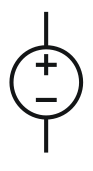
\includegraphics{ivsSymbol}}

\device
\begin{alltt}
V<name> <(+) node> <(-) node> [ [DC] <value> ]
+ [AC [magnitude value [phase value] ] ] [transient specification]
\end{alltt}

\examples
\begin{alltt}
VSLOW 1 22 SIN(0.5 1.0mV 1KHz 1ms)
VPULSE 1 3 PULSE(-1 1 2ns 2ns 2ns 50ns 100ns)
VPAT 2 4 PAT(5 0 0 1n 2n 5n b0101)
\end{alltt}


\parameters

\begin{Parameters}

\param{transient specification}

There are five predefined time-varying functions for sources:

\begin{description}
\item[\tt PULSE <parameters>] Pulse waveform
\item[\tt SIN <parameters>] Sinusoidal waveform
\item[\tt EXP <parameters>] Exponential waveform
\item[\tt PAT <parameters>] Pattern waveform
\item[\tt PWL <parameters>] Piecewise linear waveform
\item[\tt SFFM <parameters>] Frequency-modulated waveform
\end{description}

\end{Parameters}

\comments

Positive current flows from the positive node
through the source to the negative node. 

The power supplied or dissipated by the voltage source is calculated 
with $I \cdot \Delta V$ where the voltage drop is calculated as $(V_+ - V_-)$ 
and positive current flows from $V_+$ to $V_-$.  Dissipated power has a
positive sign, while supplied power has a negative sign.

None, any, or all of the DC, AC, and transient values
can be specified. The AC phase value is in degrees. 

\end{Device}

\paragraph{Transient Specifications}
This section outlines the available transient specifications. $\Delta t$ and
$T_{F}$ are the time step size and simulation end-time, respectively.
Parameters marked as -- must have a value specified for them;
otherwise a netlist parsing error will occur.

\subparagraph{Pulse}
\begin{alltt}
PULSE(V1 V2 TD TR TF PW PER)
\end{alltt}

\begin{DeviceParamTable}{Pulse Parameters}
V1 & Initial Value & Volt & -- \\ \hline
V2 & Pulse Value & Volt & 0.0 \\ \hline
TD & Delay Time & s & 0.0 \\ \hline
TR & Rise Time & s & $\Delta t$ \\ \hline
TF & Fall Time & s & $\Delta t$ \\ \hline
PW & Pulse Width & s & $T_F$ \\ \hline
PER & Period & s & $T_F$ \\ \hline
\end{DeviceParamTable}

\subparagraph{Sine}
\begin{alltt}
SIN(V0 VA FREQ TD THETA PHASE)
\end{alltt}

\begin{DeviceParamTable}{Sine Parameters}
V0 & Offset                & Volt & --   \\ \hline
VA & Amplitude             & Volt & --   \\ \hline
FREQ & Frequency           & s$^{-1}$  & --   \\ \hline
TD & Delay                 & s    & $\Delta t$ \\ \hline
THETA & Attenuation Factor & s    & $\Delta t$ \\ \hline
PHASE & Phase              & degrees & 0.0 \\ \hline 
\end{DeviceParamTable}

The waveform is shaped according to the following equations, where $\phi=\pi*\mathbf{PHASE}/180$ :
\[
V = \left\{ \begin{array}{ll}
V_0, & 0 < t < T_D \\
V_0 + V_A \sin[2\pi\cdot\mathbf{FREQ}\cdot(t - T_D)+\phi]
\exp[-(t - T_D) \cdot \mathbf{THETA}], & T_D < t < T_F
\end{array}
\right.
\]

\subparagraph{Exponent}
\begin{alltt}
EXP(V1 V2 TD1 TAU1 TD2 TAU2)
\end{alltt}

\begin{DeviceParamTable}{Exponent Parameters}
V1 & Initial Amplitude & Volt & -- \\ \hline
V2 & Amplitude & Volt & -- \\ \hline
TD1 & Rise Delay Time & s & 0.0 \\ \hline
TAU1 & Rise Time Constant & s & $\Delta t$ \\ \hline
TD2 & Delay Fall Time & s & TD1 $+ \Delta t$ \\ \hline
TAU2 & Fall Time Constant & s & $\Delta t$ \\ \hline
\end{DeviceParamTable}

The waveform is shaped according to the following equations:
\[
V = \left\{ \begin{array}{ll}
V_1, & 0 < t < \mathrm{TD1} \\
V_1 + (V_2 - V_1) \{1 - \exp[-(t-\mathrm{TD1}) / \mathrm{TAU1}] \} ,
& \mathrm{TD1} < t < \mathrm{TD2} \\
V_1 + (V_2 - V_1) \{1 - \exp[-(t- \mathrm{TD1}) / \mathrm{TAU1}] \} \\
\;\;\;\;\, + (V_1 - V_2) \{1 - \exp[-(t - \mathrm{TD2}) / \mathrm{TAU2}] \} ,
& \mathrm{TD2} < t < T_2
\end{array}
\right. \]

\subparagraph{Pattern}
\begin{alltt}
PAT(VHI VLO TD TR TF TSAMPLE DATA R)
\end{alltt}

\begin{DeviceParamTable}{Pattern Parameters}
VHI & High Value & Volt & -- \\ \hline
VLO & Low Value & Volt & -- \\ \hline
TD & Delay Time & s & -- \\ \hline
TR & Rise Time & s & -- \\ \hline
TF & Fall Time & s & -- \\ \hline
TSAMPLE & Bit period & s & -- \\ \hline
DATA & Bit pattern & -- & -- \\ \hline
R & Repeat & --  & 0 \\ \hline
\end{DeviceParamTable}

The \texttt{VHI}, \texttt{VLO}, \texttt{TD}, \texttt{TF}, \texttt{TF}
\texttt{TSAMPLE} and \texttt{DATA} parameters are all required, and
hence have no default values.  Negative values for \texttt{TD} are
supported.  The \texttt{R} parameter is optional.  For its default
value of 0, the requested bit pattern will occur once.

The \texttt{DATA} parameter is the requested bit-pattern.  Only the
0' and `1' states are supported.  The `M' and `Z' states are not
supported.  The \texttt{DATA} field should have a leading `b' (or `B')
character (e.g., be specified as `b0101' ).

For times earlier than \texttt{TD}, the waveform value is set by the
first bit in \texttt{DATA}.  For times after the end of the (possibly
repeated) pattern, the waveform value is set by the last bit in
\texttt{DATA}.  Piecewise linear interpolation is used to generate
the output value when transitioning between states.

The relationship between the various source parameters can be
illustrated with the following example:

V1 1 0 PAT(5 0 0 1n 1n 5n b010)

That V1 source definition would produce time-voltages pairs at
(0 0) (4.5ns 0) (5ns 2.5) (5.5ns 5.0) (9.5ns 5.0)
(10ns 2.5) (10.5ns 0).  So, the bit period is 5ns and the
voltage value at the start/end of each ``sample'' is equal to
0.5*(\texttt{VHI} + \texttt{VLO}).  The first rise is centered
around t=5ns, and hence starts at t=4.5ns and ends at t=5.5 ns.

The \texttt{VHI}, \texttt{VLO}, \texttt{TD}, \texttt{TF}, \texttt{TF}
and \texttt{TSAMPLE} parameters are compatible with \texttt{.STEP}.
The \texttt{DATA} and \texttt{R} parameters are not.

The HSPICE parameters \texttt{RB}, \texttt{ENCODE} and \texttt{RD\_INIT},
for the pattern source, are not supported.

\subparagraph{Piecewise Linear}
\begin{alltt}
PWL  T0 V0 [Tn Vn]*
PWL  FILE "<name>" [TD=<timeDelay>] [R=<repeatTime>]
\end{alltt}

\begin{DeviceParamTable}{Piecewise Linear Parameters}
T$_n$ & Time at Corner & s & none \\ \hline
V$_n$ & Voltage at Corner & Volt & none \\ \hline
TD & Time Delay & s & 0 \\ \hline
R & Repeat Time & s & none \\ \hline 
\end{DeviceParamTable}

When the FILE option is given, \Xyce{} will read the corner points
from the file specified in the \texttt{<name>} field.  This file
should be a plain ASCII text file (or a .CSV file) with time/voltage pairs.  
There should be one pair per line, and the time and voltage values should be
separated by whitespace or commas. As an example, the file 
specified (e.g., \texttt{vpwl.csv}) could have these five lines:
\begin{alltt}
0.00, 0.00
2.00, 3.00
3.00, 2.00
4.00, 2.00
4.01, 5.00
\end{alltt}
The corresponding example instance lines would be:
\begin{alltt}
VPWL1 1 0 PWL 0S 0V  2S 3V  3S 2V  4S 2V  4.01S 5V
VPWL2 2 0 PWL FILE "vpwl.txt"
VPWL3 3 0 PWL file "vpwl.csv"
VPWL4 4 0 PWL FILE vpwl.csv
\end{alltt}

The double quotes around the file name are optional, as shown above.

It is a best practice to specify all of the time-voltage pairs in the PWL specification.
However, for compatibility with HSPICE and PSpice, if the user-specified list of 
time/voltage pairs omits the pair at time=0 as the first pair in the list then \Xyce{} 
will insert a pair at time=0 with the voltage value at the first user-specified time value.  
As an example, this user-specified list:
\begin{alltt}
2S 3V  3S 2V  4S 2V  4.01S 5V
\end{alltt}
would be implemented in \Xyce{} as follows:  
\begin{alltt} 
0S 3V  2S 3V  3S 2V  4S 2V  4.01S 5V
\end{alltt}

TD has units of seconds, and specifies the length of time to delay
the start of PWL waveform.  The default is to have no delay, and TD is 
an optional parameter.

The Repeat Time (R) is an optional parameter.  If R is omitted then the waveform
will not repeat.  If R is included then the waveform will repeat until the end
of the simulation.  As examples, R=0 means repeat the PWL waveform from time=0
to the last time (T$_N$) specified in the waveform specification. (This would use the
time points 0s, 2s, 3s, 4s and 4.01s for the example waveform given above.)
In general, R=\texttt{<repeatTime>} means repeat the waveform from time equal to
\texttt{<repeatTime>} seconds in the waveform specification to the last time (T$_N$)
specified in the waveform specification.  So, the \texttt{<repeatTime>} must be 
greater than or equal to 0 and less than the last time point (T$_N$).
If the R parameter is used then it must have a value.  

The specification \texttt {PWL  FILE "<name>"  R}  \texttt is illegal in \Xyce{} as
a shorthand for R=0.  Also, the \Xyce{} syntax for PWL sources is not compatible
with the PSpice \texttt{REPEAT} syntax for PWL sources. See section 
\ref{PWL_SOURCE_SYNTAX_DIFF} for more details.

The repeat time (R) does enable the specification of discontinuous piecewise linear
waveforms.  For example, this waveform is a legal \Xyce{} syntax.  
\begin{alltt}
VPWL1 1 0 PWL 0S 0V  2S 3V  3S 2V  4S 2V  4.01V 5V  R=2
\end{alltt}
However, in general, discontinuous source waveforms may cause convergence problems.

\subparagraph{Frequency Modulated}
\begin{alltt}
SFFM (V0 VA FC MDI FS)
\end{alltt}

\begin{DeviceParamTable}{Frequency Modulated Parameters}
V0 & Offset & Volt & -- \\ \hline
VA & Amplitude & Volt & -- \\ \hline
FC & Carrier Frequency & hertz & 1/\textrmb{TSTOP} \\ \hline
MDI & Modulation Index & - & 0 \\ \hline
FS & Signal Frequency & hertz & 1/\textrmb{TSTOP} \\ \hline
\end{DeviceParamTable}

\textrmb{TSTOP} is the final time, as entered into the transient
(\texttt{.TRANS}) command. The waveform is shaped according to the following
equation:
\[
V = {V_0 + V_A} \cdot \sin(2\pi \cdot \mathrm{FC} \cdot \mathbf{TIME} +
\mathrm{MDI} \cdot \sin(2\pi \cdot \mathrm{FS} \cdot \mathbf{TIME}))
\]
where \textrmb{TIME} is the current simulation time.


%%
%% Voltage-Controlled Voltage-Source Section
%%

%%
%% Port device 
%%
\clearpage
\subsection{Port Device}
\index{device!port device} \index{port device}
% Sandia National Laboratories is a multimission laboratory managed and
% operated by National Technology & Engineering Solutions of Sandia, LLC, a
% wholly owned subsidiary of Honeywell International Inc., for the U.S.
% Department of Energy’s National Nuclear Security Administration under
% contract DE-NA0003525.

% Copyright 2002-2020 National Technology & Engineering Solutions of Sandia,
% LLC (NTESS).


\begin{Device}\label{P_DEVICE}

%\symbol
%{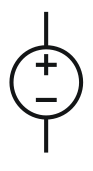
\includegraphics{ivsSymbol}}

\device
\begin{alltt}
P<name> <(+) node> <(-) node> [[DC] <value> ] port=port number
+ [Z0 = value] [AC [magnitude value [phase value] ] ]
+ [transient specification]
\end{alltt}

\examples
\begin{alltt}
P1 1 0 port = 1
P2 12 0  port=1  z0=100
P1 1 0 port=2   sin 0  1 1e5
P2 2 0 port=2 z0=100 AC 1
\end{alltt}


\parameters

\begin{Parameters}

\param{port}

The port number. Numbered sequentially beginning with 1

\param{Z0} 

System impedance. Currently, it only supports a real-valued impedance.

\param{transient specification}

There are six predefined time-varying functions for sources:

\begin{description}
\item[\tt PULSE <parameters>] Pulse waveform
\item[\tt SIN <parameters>] Sinusoidal waveform
\item[\tt EXP <parameters>] Exponential waveform
\item[\tt PAT <parameters>] Pattern waveform
\item[\tt PWL <parameters>] Piecewise linear waveform
\item[\tt SFFM <parameters>] Frequency-modulated waveform
\end{description}

\end{Parameters}

\comments

The port device identifies the ports used in .LIN analysis. Each
port requires a unique port number. For example, if the netlist has
N port devices, it must contain the sequential set of port
numbers, from 1 to N. Each port has an associated impedance Z0. The
default is 50 ohms. 

The port device behaves as a voltage source in series with an impedance
for all other analyses, such as DC, AC and transient.

None, any, or all of the DC, AC, and transient values
can be specified. The AC phase value is in degrees. The port device
accepts the same transient specifications as the voltage (V) sources.

Positive current flows from the positive node through the port
device to the negative node. 

The power supplied or dissipated by the port device is calculated 
with $I \cdot \Delta V$ where the voltage drop is calculated as $(V_+ - V_-)$ 
and positive current flows from $V_+$ to $V_-$.  Dissipated power has a
positive sign, while supplied power has a negative sign.

\end{Device}



\clearpage
\subsection{Voltage Controlled Voltage Source}
\index{device!voltage controlled voltage source} \index{voltage controlled voltage source}
\index{voltage source!voltage controlled}
% Sandia National Laboratories is a multimission laboratory managed and
% operated by National Technology & Engineering Solutions of Sandia, LLC, a
% wholly owned subsidiary of Honeywell International Inc., for the U.S.
% Department of Energy’s National Nuclear Security Administration under
% contract DE-NA0003525.

% Copyright 2002-2019 National Technology & Engineering Solutions of Sandia,
% LLC (NTESS).


\begin{Device}\label{E_DEVICE}

\symbol
{
\includegraphics{vcvsSymbol}}

\device
\begin{alltt}
E<name> <(+) node> <(-) node> <(+) controlling node>
+ <(-) controlling node> <gain>
E<name> <(+) node> <(-) node> VALUE = \{ <expression> \}  
+ [device parameters]
E<name> <(+) node> <(-) node> TABLE \{ <expression> \} = 
+ < <input value>,<output value> >*
E<name> <(+) node> <(-) node> POLY(<value>) 
+ [<+ control node> <- control node>]*
+ [<polynomial coefficient value>]*
\end{alltt}

\examples
\begin{alltt}
EBUFFER 1 2 10 11 5.0
ESQROOT   5   0 VALUE = \{5V*SQRT(V(3,2))\}
ET2 2 0 TABLE \{V(ANODE,CATHODE)\} = (0,0) (30,1)
EP1 5 1 POLY(2) 3 0 4 0 0 .5 .5
\end{alltt}

\parameters

\begin{Parameters}

\param{\vbox{\hbox{(+) node\hfil}\hbox{(-) node}}}

Output nodes. Positive current flows from the \texttt{(+)} node through
the source to the \texttt{(-)} node.

\param{\vbox{\hbox{(+) controlling node\hfil}\hbox{(-) controlling node}}}

Node pairs that define a set of controlling voltages. A given node may
appear multiple times and the output and controlling nodes may be the
same.


\param{device parameters} 

The second form supports two instance parameters \texttt{smoothbsrc} and
\texttt{rcconst}. Parameters may be provided as space separated
\texttt{<parameter>=<value>} specifications as needed. The default value for
\texttt{smoothbsrc} is 0 and the default for \texttt{rcconst} is 1e-9.

\end{Parameters}

\comments 

In the first form, a specified voltage drop between controlling nodes is
multiplied by the gain to determine the voltage drop across the output nodes. 

The second through fourth forms allow nonlinear controlled sources using the
\texttt{VALUE}, \texttt{TABLE}, or \texttt{POLY} keywords, respectively, and
are used in analog behavioral modeling.  They are provided primarily for
netlist compatibility with other simulators.  These three forms are
automatically converted within \Xyce{} to its principal ABM device, the
\texttt{B} nonlinear dependent source device. See the B-source section
(\ref{B_Source_Device}) and the \Xyce{} User's Guide for more guidance on
analog behavioral modeling.  For details concerning the use of the
\texttt{POLY} format, see section~\ref{PspicePoly}.

For HSPICE compatibility, \texttt{VOL} is an allowed synonym for
\texttt{VALUE} for the E-source.

The power supplied or dissipated by this source device is calculated 
with $I \cdot \Delta V$ where the voltage drop is calculated as $(V_+ - V_-)$ 
and positive current flows from $V_+$ to $V_-$.  Dissipated power has a
positive sign, while supplied power has a negative sign.

{\bf NOTE:} The expression given on the left hand side of the equals
sign in E source TABLE expressions may be enclosed in braces, but is
not required to be.  Further, if braces are present there must be
exactly one pair of braces and it must enclose the entire expression.
It is not legal to use additional pairs of braces as parentheses
inside these expressions.  So
\begin{alltt}
ET2 2 0 TABLE \{V(ANODE,CATHODE)+5\} = (0,0) (30,1)
ET3 2 0 TABLE V(ANODE,CATHODE)+5 = (0,0) (30,1)
\end{alltt}
are legal, but 
\begin{alltt}
ET2 2 0 TABLE \{V(ANODE,CATHODE)+\{5\}\} = (0,0) (30,1)
\end{alltt}
is not.  This last will result in a parsing error about missing braces.
\end{Device}


%%
%% Current-Controlled Current-Source Section
%%
\clearpage
\subsection{Current Controlled Current Source}
\index{device!current controlled current source} \index{current controlled current source}
\index{current source!current controlled}
% Sandia National Laboratories is a multimission laboratory managed and
% operated by National Technology & Engineering Solutions of Sandia, LLC, a
% wholly owned subsidiary of Honeywell International Inc., for the U.S.
% Department of Energy’s National Nuclear Security Administration under
% contract DE-NA0003525.

% Copyright 2002-2020 National Technology & Engineering Solutions of Sandia,
% LLC (NTESS).


\begin{Device}

\symbol
{
\includegraphics{cccsSymbol}}

\device
\begin{alltt}
F<name> <(+) node> <(-) node>
+ <controlling V device name> <gain>
F<name> <(+) node> <(-) node> POLY(<value>)
+ <controlling V device name>*
+ < <polynomial coefficient value> >*
\end{alltt}

\examples
\begin{alltt}
FSENSE 1 2 VSENSE 10.0
FAMP 13 0 POLY(1) VIN 0 500
FNONLIN 100 101 POLY(2) VCNTRL1 VCINTRL2 0.0 13.6 0.2 0.005
\end{alltt}

\parameters

\begin{Parameters}

\param{\vbox{\hbox{(+) node\hfil}\hbox{(-) node}}}
Output nodes. Positive current flows from the \texttt{(+)} node through
the source to the \texttt{(-)} node.

\param{controlling V device}
The controlling voltage source which must be an independent voltage source
(V device).

\end{Parameters}

\comments

In the first form, a specified current through a controlling device is
multiplied by the gain to determine this device's output current.  The
gain may be expressed either as a number, a parameter, or an arbitrary
brace-delimited ABM expression.

The second form using the \texttt{POLY} keyword is used in analog behavioral
modeling.

Both forms are automatically converted within \Xyce{} to its principal
ABM device, the \texttt{B} nonlinear dependent source device. See the B-source
section (\ref{B_Source_Device}) and the \Xyce{} User's Guide for more guidance
on analog behavioral modeling.  For details concerning the use of the
\texttt{POLY} format, see section~\ref{PspicePoly}.

The power supplied or dissipated by this source device is calculated 
with $I \cdot \Delta V$ where the voltage drop is calculated as $(V_+ - V_-)$ 
and positive current flows from $V_+$ to $V_-$.  Dissipated power has a
positive sign, while supplied power has a negative sign.

F-sources were originally developed primarily to support DC and transient analysis.  
As such, their support for frequency domain analysis (AC and HB) has some limitations.  
The main limitation to be aware of is that time-dependent sources will not work with AC or HB analysis.  
These are sources in which the variable \alltt{TIME} is used in the \alltt{VALUE=} expression. 
However, this time-dependent usage is not common.  The most 
common use case is one in which the F-source is purely dependent (depends only 
on other solution variables), and this use case will work with AC and HB.  

\end{Device}


%%
%% Voltage-Controlled Current-Source Section
%%
\clearpage
\subsection{Voltage Controlled Current Source}
\index{device!voltage controlled current source} \index{voltage controlled current source}
\index{current source!voltage controlled}
% Sandia National Laboratories is a multimission laboratory managed and
% operated by National Technology & Engineering Solutions of Sandia, LLC, a
% wholly owned subsidiary of Honeywell International Inc., for the U.S.
% Department of Energy’s National Nuclear Security Administration under
% contract DE-NA0003525.

% Copyright 2002-2021 National Technology & Engineering Solutions of Sandia,
% LLC (NTESS).



\begin{Device}\label{G_DEVICE}

\symbol
{
\includegraphics{vccsSymbol}}

\device
\begin{alltt}
G<name> <(+) node> <(-) node> <(+) controlling node>
+ <(-) controlling node> <transconductance>
G<name> <(+) <node> <(-) node> VALUE = \{ <expression> \}
G<name> <(+) <node> <(-) node> TABLE \{ <expression> \} =
+ < <input value>,<output value> >*
G<name> <(+) <node> <(-) node> POLY(<value>)
+ [<+ controlling node> <- controlling node>]*
+ [<polynomial coefficient>]*
\end{alltt}

\examples
\begin{alltt}
GBUFFER 1 2 10 11 5.0
GPSK 11 6 VALUE = \{5MA*SIN(6.28*10kHz*TIME+V(3))\}
GA2 2 0 TABLE \{V(5)\} = (0,0) (1,5) (10,5) (11,0)
\end{alltt}

\parameters

\begin{Parameters}

\param{\vbox{\hbox{(+) node\hfil}\hbox{(-) node}}}

Output nodes. Positive current flows from the \texttt{(+)} node through
the source to the \texttt{(-)} node.

\param{\vbox{\hbox{(+) controlling node\hfil}\hbox{(-) controlling node}}}

Node pairs that define a set of controlling voltages. A given node may
appear multiple times and the output and controlling nodes may be the
same.

\end{Parameters}

\comments

In the first form, the voltage drop between the controlling nodes is
multiplied by the transconductance to obtain the current-source
output of the \texttt{G} device. 

The second through fourth forms using the \texttt{VALUE}, \texttt{TABLE}, and
\texttt{POLY} keywords, respectively, are used in analog behavioral modeling.
They are provided primarily for netlist compatibility with other simulators.
These two forms are automatically converted within \Xyce{} to its principal ABM
device, the B nonlinear dependent source device. See the B-source section
(\ref{B_Source_Device}) and the \Xyce{} User's Guide for more guidance on
analog behavioral modeling.  For details concerning the use of the
\texttt{POLY} format, see section~\ref{PspicePoly}.

For HSPICE compatibility, \texttt{CUR} is an allowed synonym for
\texttt{VALUE} for the G-source.

The power supplied or dissipated by this source device is calculated 
with $I \cdot \Delta V$ where the voltage drop is calculated as $(V_+ - V_-)$ 
and positive current flows from $V_+$ to $V_-$.  Dissipated power has a
positive sign, while supplied power has a negative sign.

{\bf NOTE:} The expression given on the left hand side of the equals
sign in G source TABLE expressions may be enclosed in braces, but is
not required to be.  Further, if braces are present there must be
exactly one pair of braces and it must enclose the entire expression.
It is not legal to use additional pairs of braces as parentheses
inside these expressions.  So
\begin{alltt}
GA2 2 0 TABLE \{V(5)+5\} = (0,0) (1,5) (10,5) (11,0)
GA3 2 0 TABLE V(5) = (0,0) (1,5) (10,5) (11,0)
\end{alltt}
are legal, but
\begin{alltt}
GA2 2 0 TABLE \{V(5)+\{5\}\} = (0,0) (1,5) (10,5) (11,0)
\end{alltt}
is not.  This last will result in a parsing error.

G-sources were originally developed primarily to support DC and transient analysis.  
As such, their support for frequency domain analysis (AC and HB) has some limitations.  
The main limitation to be aware of is that time-dependent sources will not work with AC or HB analysis.  
These are sources in which the variable \texttt{TIME} is used in the \texttt{VALUE=} expression. 
However, this time-dependent usage is not common.  The most 
common use case is one in which the G-source is purely dependent (depends only 
on other solution variables), and this use case will work with AC and HB.  
\end{Device}



%%
%% Current-Controlled Voltage-Source Section
%%
\clearpage
\subsection{Current Controlled Voltage Source}
\index{device!current controlled voltage source} \index{current controlled voltage source}
\index{voltage source!current controlled}
% Sandia National Laboratories is a multimission laboratory managed and
% operated by National Technology & Engineering Solutions of Sandia, LLC, a
% wholly owned subsidiary of Honeywell International Inc., for the U.S.
% Department of Energy’s National Nuclear Security Administration under
% contract DE-NA0003525.

% Copyright 2002-2020 National Technology & Engineering Solutions of Sandia,
% LLC (NTESS).


The syntax of this device is exactly the same as for a Current-Controlled
Current Source.  For a Current-Controlled Voltage Source just substitute an H
for the F. The H device generates a voltage, whereas the F device generates a
current.

\begin{Device}

\symbol
{
\includegraphics{ccvsSymbol}}

\device
\begin{alltt}
H<name> <(+) node> <(-) node>
+ <controlling V device name> <transresistance>
H<name> <(+) node> <(-) node> POLY(<value>)
+ <controlling V device name>*
+ < <polynomial coefficient value> >*
\end{alltt}

\examples
\begin{alltt}
HSENSE 1 2 VSENSE 10.0
HAMP 13 0 POLY(1) VIN 0 500
HNONLIN 100 101 POLY(2) VCNTRL1 VCINTRL2 0.0 13.6 0.2 0.005
\end{alltt}

\comments

In the first form, the current through a specified controlling voltage
source is multiplied by the transresistance to obtain the
voltage-source output.  The transresistance may be expressed either as
a number, a parameter, or an arbitrary brace-delimited ABM expression.

The second form using the \texttt{POLY} keyword is used in analog
behavioral modeling.  It is provided primarily for netlist
compatibility with other simulators.

H sources in any form are automatically converted within \Xyce{} to
its principal ABM device, the B nonlinear dependent source device. See
the B-source section (\ref{B_Source_Device}) and the \Xyce{} User's
Guide for more guidance on analog behavioral modeling.  For details
concerning the use of the \texttt{POLY} format, see
section~\ref{PspicePoly}.

The power supplied or dissipated by this source device is calculated
with $I \cdot \Delta V$ where the voltage drop is calculated as $(V_+ - V_-)$
and positive current flows from $V_+$ to $V_-$.  Dissipated power has a
positive sign, while supplied power has a negative sign.

H-sources were originally developed primarily to support DC and transient analysis.  
As such, their support for frequency domain analysis (AC and HB) has some limitations.  
The main limitation to be aware of is that time-dependent sources will not work with AC or HB analysis.  
These are sources in which the variable \alltt{TIME} is used in the \alltt{VALUE=} expression. 
However, this time-dependent usage is not common.  The most 
common use case is one in which the H-source is purely dependent (depends only 
on other solution variables), and this use case will work with AC and HB.  

\end{Device}


%%
%% BSource Section
%%
\clearpage
\subsection{Nonlinear Dependent Source}
\label{B_Source_Device}
\index{device!bsource} \index{bsource}
\index{voltage source!nonlinear dependent} \index{current source!nonlinear dependent}
% Sandia National Laboratories is a multimission laboratory managed and
% operated by National Technology & Engineering Solutions of Sandia, LLC, a
% wholly owned subsidiary of Honeywell International Inc., for the U.S.
% Department of Energy’s National Nuclear Security Administration under
% contract DE-NA0003525.

% Copyright 2002-2021 National Technology & Engineering Solutions of Sandia,
% LLC (NTESS).


\begin{Device}\label{B_DEVICE}

\device
\begin{alltt}
B<name> <(+) node> <(-) node> V={ABM expression} [device parameters]
B<name> <(+) node> <(-) node> I={ABM expression}
\end{alltt}

\examples
\begin{alltt}
B1 2 0 V=\{sqrt(V(1))\}
B2 4 0 V=\{V(1)*TIME\}
B3 4 2 I=\{I(V1) + V(4,2)/100\}
B4 5 0 V=\{Table \{V(5)\}=(0,0) (1.0,2.0) (2.0,3.0) (3.0,10.0)\}
B5 6 0 V=tablefile("file.dat")
B6 7 0 I=tablefile("file.dat")
\end{alltt}

\comments

The nonlinear dependent source device, also known as the B-source
device, is used in analog behavioral modeling (ABM).  The \texttt{(+)}
and \texttt{(-)} nodes are the output nodes. Positive current flows from
the \texttt{(+)} node through the source to the \texttt{(-)}
node. 

The power supplied or dissipated by the nonlinear dependent source is calculated 
with $I \cdot \Delta V$ where the voltage drop is calculated as $(V_+ - V_-)$ 
and positive current flows from $V_+$ to $V_-$.  Dissipated power has a
positive sign, while supplied power has a negative sign.

The syntax involving the \texttt{tablefile} keyword internally attempts to load the
data in \texttt{"file.dat"} into a \texttt{TABLE} expression.  The data file must
be in plain-text and contain just two pairs of data per line.  For an example see 
the ``Analog Behavioral Modeling'' chapter of the \Xyce{} User's
Guide.

It is important to note that the B-source allows the user to specify
expressions that could have infinite-slope transitions, such as the
following.  (Note: the braces surrounding all expressions are required in this definition.)
\begin{alltt} Bcrtl OUTA 0 V=\{ IF( (V(IN) > 3.5), 5, 0 ) \} \end{alltt}
This can lead to ``timestep too small'' errors when \Xyce{} reaches the
transition point.  Infinite-slope transitions in expressions dependent only on
the \texttt{time} variable are a special case, because \Xyce{} can detect that
they are going to happen in the future and set a ``breakpoint'' to capture
them.  Infinite-slope transitions depending on other solution variables cannot
be predicted in advance, and cause the time integrator to scale back the
timestep repeatedly in an attempt to capture the feature until the timestep is
too small to continue.

One solution to the problem is to modify the expression to allow a continuous transition. 
However, this can become complicated with multiple inputs. The other solution is to specify
device options or instance parameters to allow smooth transitions. The parameter
\texttt{smoothbsrc} enables the smooth transitions. This is done by adding a RC network to the  
output of B sources. For example,

\begin{alltt} Bcrtl OUTA 0 V=\{ IF( (V(IN) > 3.5), 5, 0 ) \} smoothbsrc=1 \end{alltt}

\begin{alltt} .options device  smoothbsrc=1 \end{alltt}

The smoothness of the transition can be controlled by specifying the rc constant of 
the RC network. For example, 

\begin{alltt} Bcrtl OUTA 0 V=\{ IF( (V(IN) > 3.5), 5, 0 ) \} smoothbsrc=1   
 + rcconst = 1e-10 \end{alltt}

Note that this smoothed B-source only applies to voltage sources. The voltage behavioral source supports
two instance parameters \texttt{smoothbsrc} and \texttt{rcconst}. Parameters may be provided as space  
separated \texttt{<parameter>=<value>} specifications as needed. The default value for \texttt{smoothbsrc}
is 0 and the default for \texttt{rcconst} is 1e-9.

See the ``Analog Behavioral Modeling'' chapter of the \Xyce{} User's
Guide for guidance on using the B-source device and ABM expressions,
and the Expressions Section (\ref{ExpressionDocumentation}) for
complete documentation of expressions and expression operators.
One important note is that time-dependent expressions are supported
for the current and voltage parameters of a B source, but
frequency-dependent expressions are not.

B-sources were originally developed primarily to support DC and transient analysis.  
As such, their support for frequency domain analysis (AC and HB) has some limitations.  
The main limitation to be aware of is that time-dependent sources will not work with AC or HB analysis.  
These are sources in which the variable \texttt{TIME} is used in the \texttt{VALUE=} expression. 
The use case of a purely depedent B-source (depends only on other solution variables) will work with AC and HB.  

\end{Device}


%%
%% BJT Section
%%
\clearpage
\subsection{Bipolar Junction Transistor (BJT)}
\index{device!BJT} \index{BJT}
% Sandia National Laboratories is a multimission laboratory managed and
% operated by National Technology & Engineering Solutions of Sandia, LLC, a
% wholly owned subsidiary of Honeywell International Inc., for the U.S.
% Department of Energy’s National Nuclear Security Administration under
% contract DE-NA0003525.

% Copyright 2002-2020 National Technology & Engineering Solutions of Sandia,
% LLC (NTESS).


%%
%% BJT Description Table
%%

\begin{Device}\label{Q_DEVICE}

\symbol
{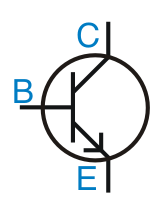
\includegraphics{npnSymbol}}
{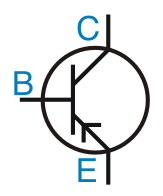
\includegraphics{pnpSymbol}}

\device
\begin{alltt}
Q<name> <collector node> <base node> <emitter node>
 + [substrate node] <model name> [area value]

Q<name> <collector node> <base node> <emitter node>
 + [thermal node] <VBIC 1.3 3-terminal model name>

Q<name> <collector node> <base node> <emitter node>
 + <substrate> [thermal node] <VBIC 1.3 4-terminal model name>

 Q<name> <collector node> <base node> <emitter node>
 + <substrate> <thermal node> <HICUM model name>
\end{alltt}

\model
\begin{alltt}
.MODEL <model name> NPN [model parameters]
.MODEL <model name> PNP [model parameters]
\end{alltt}

\examples
\begin{alltt}
Q2 10 2 9 PNP1
Q12 14 2 0 1 NPN2 2.0
Q6 VC 4 11 [SUB] LAXPNP
Q7 Coll Base Emit DT VBIC13MODEL2
Q8 Coll Base Emit VBIC13MODEL3 SW\_ET=0
Q9 Coll Base Emit Subst DT VBIC13MODEL4
Q10 Coll Base Emit Subst DT HICUMMMODEL1
\end{alltt}

\parameters
\begin{Parameters}
\param{substrate node}
  Optional and defaults to ground. Since \Xyce{} permits alphanumeric
  node names and because there is no easy way to make a distinction between
  these and the model names, the name (not a number) used for the substrate
  node must be enclosed in square brackets \texttt{[ ]}.  Otherwise, nodes
  would be interpreted as model names. See the fourth example above.

\param{area value}
  The relative device area with a default value of 1.

\end{Parameters}

\comments
The BJT is modeled as an intrinsic transistor using ohmic resistances in series
with the collector (RC/area), with the base (value varies with current, see BJT
equations) and with the emitter (RE/area).For model parameters with optional
names, such as VAF and VA (the optional name is in parentheses), either may be
used.For model types NPN and PNP, the isolation junction capacitance is
connected between the intrinsic-collector and substrate nodes. This is the same
as in SPICE and works well for vertical IC transistor structures.

\textbf{Only the VBIC 1.3 model is available in \Xyce{} 6.11 and
  later.}  The VBIC 1.3 model is provided in both 3-terminal (Q level
  11) and 4-terminal (Q level 12) variants, both supporting
  electrothermal and excess-phase effects.  These variants of the Q line
  are shown in the fourth through sixth examples above. VBIC 1.3
  instance lines have three or four required nodes, depending on model
  level, and an \emph{optional} ``dt'' node.  The first three are the
  normal collector, base,and emitter. In the level 12 (4-terminal) the
  fourth node is the substrate, just as for the level 1 BJT.  If the
  optional ``dt'' node is specified for either variant, it can be used
  to print the local temperature rise due to self-heating, and could
  possibly be used to model coupled heating effects of several VBIC
  devices.  It is, however, unnecessary to specify a ``dt'' node just
  to print the local temperature rise, because when this node is
  omitted from the instance line it simply becomes and internal node,
  and may still be printed using the syntax
  \texttt{N(instancename:dt)}.  For the ``Q8'' example above, one
  could print \texttt{N(Q8:dt)}.

As of release 6.10 of Xyce, the VBIC 1.3 3-terminal device (Q level
11) has been the subject of extensive optimization, and runs much
faster than in previous releases.

\textbf{ The HICUM models require both a substrate and thermal node.}

\end{Device}


% BJT model schematic.
\begin{figure}[ht]
  \centering
  \scalebox{0.6}
  {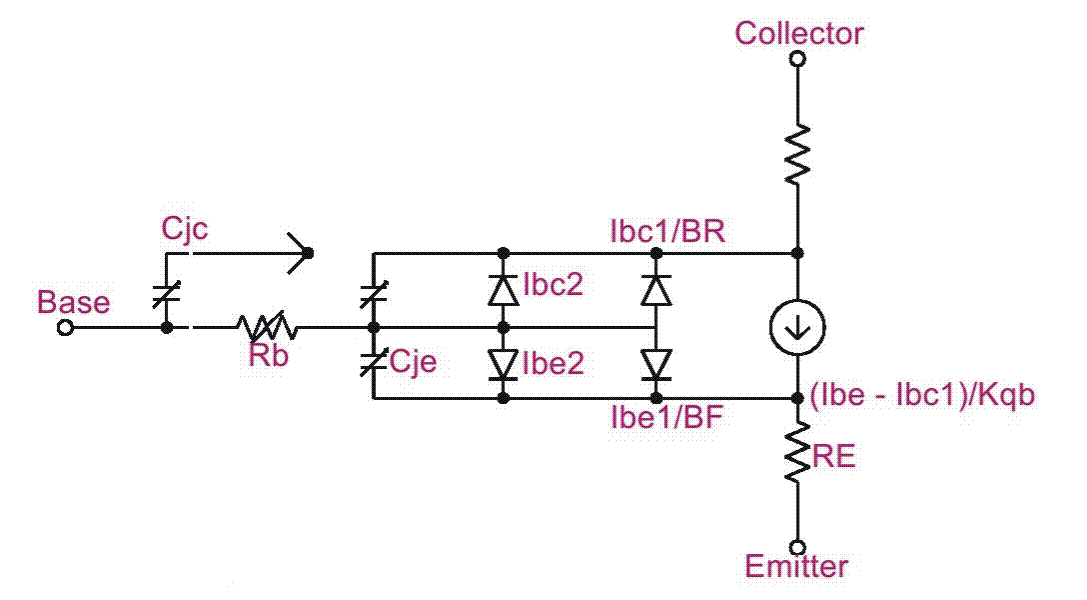
\includegraphics{bjtSchematic}}
  \caption[BJT model schematic]{BJT model schematic.  Adapted from
reference~\cite{PSpiceUG:1998}. \label{figBJTschematic}}
\end{figure}

\paragraph{BJT Level selection}

\Xyce{} supports the level 1 BJT model, which is based on the
documented standard SPICE 3F5 BJT model, but was coded independently
at Sandia.  It is mostly based on the classic Gummel-Poon BJT
model~\cite{GummelPoon}.

Two variants of the VBIC model are provided as BJT levels 11  and 12.
Levels 11 and 12 are the
3-terminal and 4-terminal variants of the VBIC 1.3.

An experimental release of the FBH HBT\_X model version
2.1\cite{Rudolph_documentationof} is provided as BJT level 23.

Both the HICUM/L0 (level 230) and HICUM/L2 (level 234) models are also
provided (\url{https://www.iee.et.tu-dresden.de/iee/eb/hic_new/hic_start.html}).

The MEXTRAM\cite{MEXTRAM_home} BJT model version 504.12.1 model is provided.
Two variants of this model are available: the level 504 model without
self-heating and without external substrate node, and the level 505 model with
self heating but without external substrate node.  The level 505 instance line
requires a fourth node for the 'dt' node, similar to the usage in all of the
VBIC models (levels 11-12), but is otherwise identical to the level 504 model.

\paragraph{BJT Power Calculations}
Power dissipated in the transistor is calculated with
$|I_{B}*V_{BE}|+|I_{C}*V_{CE}|$, where $I_{B}$ is the base current, $I_{C}$ is
the collector current, $V_{BE}$ is the voltage drop between the base and the
emitter and $V_{CE}$ is the voltage drop between the collector and the emitter.
This formula may differ from other simulators.

\subsubsection{The Level 1 Model}
\paragraph{BJT Equations}\label{bjt_equations}
The Level 1 BJT implementation within \Xyce{} is based on \cite{Fjeldly:1998}.
The equations in this section describe an NPN transistor. For the PNP device,
reverse the signs of all voltages and currents.  The equations use the
following variables:
%insert variables here
\begin{eqnarray*}
V_{be} & = & \mbox{intrinsic base-intrinsic emitter voltage} \\
V_{bc} & = & \mbox{intrinsic base-intrinsic collector voltage} \\
V_{bs} & = & \mbox{intrinsic base-substrate voltage} \\
V_{bw} & = & \mbox{intrinsic base-extrinsic collector voltage
(quasi-saturation only)} \\
V_{bx} & = & \mbox{extrinsic base-intrinsic collector voltage} \\
V_{ce} & = & \mbox{intrinsic collector-intrinsic emitter voltage} \\
V_{js} & = & \mbox{(NPN) intrinsic collector-substrate voltage} \\
&        = & \mbox{(PNP) intrinsic substrate-collector voltage} \\
% THIS DOESN'T EXIST IN XYCE
%&        = & \mbox{(LPNP) intrinsic base-substrate voltage} \\
V_{t}  & = & \mbox{$kT/q$ (thermal voltage)} \\
V_{th} & = & \mbox{threshold voltage} \\
k      & = & \mbox{Boltzmann's constant} \\
q      & = & \mbox{electron charge} \\
T      & = & \mbox{analysis temperature (K)} \\
T_{0}  & = & \mbox{nominal temperature (set using \textrmb{TNOM} option)}
\end{eqnarray*}
Other variables are listed above in BJT Model Parameters.

\subparagraph{DC Current}
The BJT model is based on the Gummel and Poon model~\cite{Grove:1967} where the
different terminal currents are written
%insert equations here
\begin{eqnarray*}
I_{e} & = & -I_{cc} - I_{be} + I_{re} + (C_{dife} +C_{de})\frac{dV_{be}}{dt} \\
I_{c} & = & -I_{cc} + I_{bc} - I_{rc} - (C_{difc}+ C_{dc})\frac{dV_{bc}}{dt} \\
I_b & = & I_e -I_c
\end{eqnarray*}
Here, $C_{dife}$ and $C_{difc}$ are the capacitances related to the hole
charges per unit area in the base, $Q_{dife}$ and $Q_{difc}$,
affiliated with the electrons introduced across the emitter-base and
collector-base junctions, respectively.  Also, $C_{be}$ and $C_{bc}$ are the
capacitances related to donations to the hole charge of the base, $Q_{be}$ and
$Q_{bc}$,  affiliated with the differences in the depletion regions of the
emitter-base and collector-base junctions, respectively.  The
intermediate currents used are defined as
%insert equations here
\begin{eqnarray*}
-I_{be} & = & \mathbf{\frac{IS}{BF}} \left[\exp \left(\frac{V_{be}}
{\mathbf{NF}V_{th}} \right) -1 \right] \\
-I_{cc} & = & \frac{Q_{bo}}{Q_{b}}\mathbf{IS} \left[\exp \left(\frac{V_{be}}
{\mathbf{NF} V_{th}} \right) -
\exp \left(\frac{V_{bc}}{\mathbf{NF}V_{th}} \right) \right] \\
-I_{bc} & = & \mathbf{\frac{IS}{BR}} \left[\exp \left(\frac{V_{bc}}
{\mathbf{NR}V_{th}} \right) - 1 \right] \\
I_{re} & = & \mathbf{ISE} \left[\exp \left(\frac{V_{be}}
{\mathbf{NE} V_{th}} \right) - 1 \right] \\
I_{rc} & = & \mathbf{ISC} \left[\exp \left(\frac{V_{bc}}
{\mathbf{NC}V_{th}} \right) - 1 \right]
\end{eqnarray*}
where the last two terms are the generation/recombination currents related to
the emitter and collector junctions, respectively.  The charge $Q_{b}$ is the
majority carrier charge in the base at large injection levels and is a key
difference in the Gummel-Poon model over the earlier Ebers-Moll model.  The
ratio $Q_b/Q_{bo}$ (where $Q_{bo}$ represents the zero-bias base charge, i.e.
the value of $Q_b$ when $V_{be}=V_{bc}=0$) as computed by \Xyce{} is given by
\[\frac{Q_b}{Q_{bo}} = \frac{q_1}{2}\left(1+\sqrt{1+4q_2}\right)\]
where
\begin{eqnarray*}
q_1 & = & \left(1-\frac{V_{be}}{\mathbf{VAR}}-\frac{V_{bc}}{\mathbf{VAF}}
\right)^{-1} \\
q_2 & = & \frac{\mathbf{IS}}{\mathbf{IKF}}\left[\exp\left(\frac{V_{be}}
{\mathbf{NF}V_{th}}\right)-1\right] + \frac{\mathbf{IS}}{\mathbf{IKR}}
\left[\exp\left(\frac{V_{bc}}{\mathbf{NR}V_{th}}\right)-1\right]
\end{eqnarray*}

\subparagraph{Capacitance Terms}
The capacitances listed in the above DC $I-V$ equations each consist of a
depletion layer capacitance $C_{d}$ and
a diffusion capacitance $C_{dif}$.  The first is given by
\[
C_d = \left\{
\begin{array}{ll}
\mathbf{CJ} \left(1 - \frac{V_{di}}{\mathbf{VJ}} \right)^{\mathbf{-M}} &
V_{di} \leq \mathbf{FC \cdot VJ} \\
\mathbf{CJ} \left(1 - \mathbf{FC} \right)^{-(1+\mathbf{M})} \
\left[1 - \mathbf{FC}(1 + \mathbf{M}) + \mathbf{M}
\frac{V_{di}}{\mathbf{VJ}} \right]
& V_{di} > \mathbf{FC \cdot VJ}
\end{array}
\right. \]

where $\mathbf{CJ}=\mathbf{CJE}$ for $C_{de}$, and where $\mathbf{CJ}=
\mathbf{CJC}$ for $C_{dc}$.
The diffusion capacitance (sometimes referred to as the transit time
capacitance) is
\[
C_{dif} = \mathbf{TT} G_d = \mathbf{TT} \frac{dI}{dV_{di}}
\]
where $I$ is the diode DC current given, $G_d$ is the corresponding junction
conductance, and where $\mathbf{TT}=\mathbf{TF}$ for $C_{dife}$ and
$\mathbf{TT}=\mathbf{TR}$ for $C_{difc}$.

\subparagraph{Temperature Effects}
SPICE temperature effects are default, but all levels of the BJT have a more
advanced temperature compensation available.  By specifying
\texttt{TEMPMODEL=QUADRATIC} in the netlist, parameters can be interpolated
quadratically between measured values extracted from data.  In the BJT, IS and
ISE are interpolated logarithmically because they can change over an order of
magnitude or more for temperature ranges of interest.  See the
Section~\ref{Model_Interpolation} for more details on how to include quadratic
temperature effects.

% \subparagraph{Noise}
% Noise is calculated with a 1.0 Hz bandwidth using the following spectral power
% densities (per unit bandwidth).

% Thermal Noise due to Parasitic Resistance: $I_{n}^{2} =
% \frac{4kT}{\mathbf{RS}/area}$

% Intrinsic Diode Shot and Flicker Noise: $I_{n}^{2} = 2qI_{D} +
% \mathbf{KF}\cdot\frac{I_{D}^{\mathbf{AF}}}{\omega}$

For further information on BJT models, see~\cite{Grove:1967}.  For a thorough
description of the U.C. Berkeley SPICE models see
Reference~\cite{Antognetti:1988}.

\subsubsection{VBIC Temperature Considerations}
\index{VBIC (temperature considerations)}
The VBIC (Q levels 11 and 12) model both support a self-heating
model.  The model works by computing the power dissipated by all
branches of the device, applying this power as a flow through a small
thermal network consisting of a power flow (``current'') source
through a thermal resistance and thermal capacitance, as shown in
Figure~\ref{vbicthermal}.  The circuit node DT will therefore be the
``thermal potential'' (temperature) across the parallel thermal
resistance and capacitance.  This temperature is the temperature rise
due to self heating of the device, which is added to the ambient
temperature and \texttt{TRISE} parameter to obtain the device
operating temperature.
\begin{figure}
  \centering
  \scalebox{0.3}
  {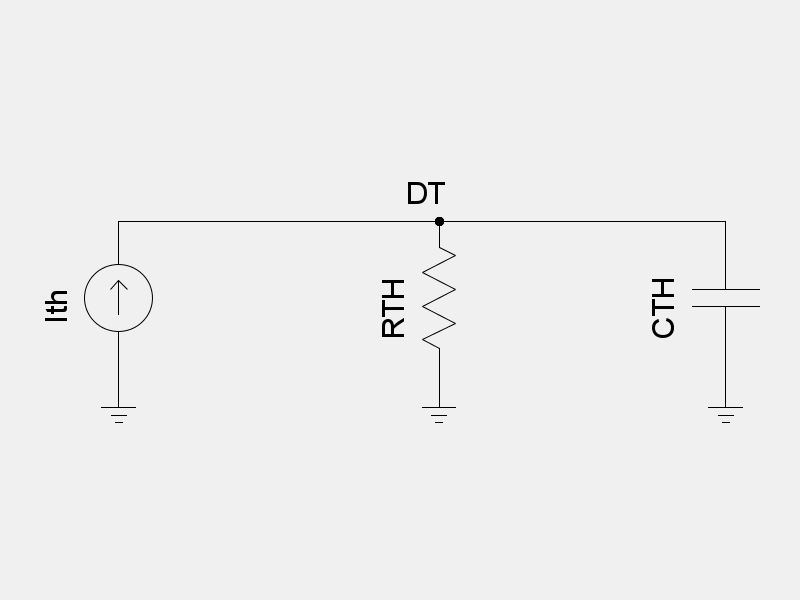
\includegraphics{VBIC_Thermal_Net}}
  \caption[VBIC thermal network schematic]{VBIC thermal network  schematic.}
  \label{vbicthermal}
\end{figure}

In VBIC 1.3, the dt node is optional on the netlist line.  If not
given, the dt node is used internally for thermal effects
calculations, but not accessible from the rest of the netlist.  The
VBIC 1.3 provides an instance parameter \texttt{SW\_ET} that may be
set to zero to turn off electrothermal self-heating effects.  When set
to zero, no thermal power is sourced into the dt node.  This parameter
defaults to 1, meaning that thermal power is computed and flows into
dt even when dt is unspecified on the netlist and remains an internal
node.

In VBIC 1.3, setting RTH to zero does {\em NOT\/} disable the
self-heating model, and does not short the dt node to ground, even
though one might expect that to be the behavior.  Rather, it simply
removes the RTH resistor from the equivalent circuit of
figure~\ref{vbicthermal} and leaves the dt node floating.  This is an
important point to recognize when using the VBIC.

If a node name is given as the fourth node of a VBIC \Xyce{} will emit
warnings about the node not having a DC path to ground and being
connected to only one device.  These warnings may safely be ignored,
and are a harmless artifact of Xyce's connectivity checker.  It is
possible to silence this warning by adding a very large resistance
between the dt node and ground --- 1GOhm or 1TOhm are effectively the
same as leaving the node floating, and will satisfy the connectivity
checker's tests.  This used to be the recommended means of silencing
the connectivity checker for the VBIC 1.2 where dt was a required
node, but it is safe {\em if and only if a nonzero\/} \texttt{RTH}
{\em value is specified for the device.}  If, however, RTH is zero,
then dt would otherwise be floating and your external resistance now
becomes the primary path for thermal power flow; rather than turning
off self-heating effects, it will be as if you had set RTH to a very
large value.  We therefore recommend that you not tie the dt node to
ground via a resistor, and if you are not using it to connect VBIC
devices together via a thermal network, simply leave off the dt node
to silence the connectivity checker warning.  Turn off self-heating
effects ONLY by setting the \texttt{SW\_ET} instance parameter to zero.

Users of earlier versions of \Xyce{} may have been using the VBIC 1.2
model that was removed in release 6.11.  All netlists containing the
old level=10 VBIC 1.2 model must be modified to run in \Xyce{} 6.11
and later.  The following points should be observed when converting an
old VBIC 1.2 netlist and model card to VBIC 1.3.

\begin{itemize}
  \item Generally speaking, most VBIC 1.2 model cards can be converted
    to VBIC 1.3 model cards by the simple substitution of
    \texttt{level=11} for \texttt{level=10}, with the following provisos.

  \item VBIC 1.2 in \Xyce{} 6.10 and earlier did not support excess
    phase effects, and so the \texttt{TD} parameter governing excess
    phase was ignored.

    The \Xyce{} team has observed that some users' VBIC 1.2 parameter
    extractions have a non-zero value for the \texttt{TD} parameter.
    The impact of this is twofold:
    \begin{itemize}
      \item Circuits that use such model cards with only the level
        number changed will likely not produce identical results when
        compared to simulation results of older versions of \Xyce{}
        using VBIC 1.2 due to the excess phase effects.  If strict
        comparison between VBIC 1.3 runs with \Xyce{} 6.11 or later
        against older runs with VBIC 1.2 is desired, change the
        \texttt{TD} parameter to zero.  This will disable the excess
        phase effects and make VBIC 1.3 equivalent to the VBIC 1.2
        that was previously provided.
      \item The \Xyce{} team has seen some instances where the
        previously ignored \texttt{TD} parameter value is such that
        \Xyce{} will fail to converge when the equivalent VBIC 1.3
        model is substituted.  The VBIC 1.2 behavior can be recovered
        by setting the model parameter \texttt{TD} to zero, which will
        disable the excess phase effect in VBIC 1.3.  We can only
        suggest that the model card be re-extracted using VBIC 1.3 to
        determine the correct value for \texttt{TD}.
    \end{itemize}

  \item VBIC 1.2 had a model parameter called \texttt{DTEMP}, which
    \Xyce{} also recognized on the instance line.  In VBIC 1.3 this
    parameter has been replaced by another called \texttt{TRISE},
    which is only an instance parameter, and is unrecognized in model
    cards.  VBIC 1.3 also recognizes \texttt{DTEMP} on the instance
    line as an alias for \texttt{TRISE}.  If you had been specifying
    \texttt{DTEMP} in your VBIC 1.2 model cards, you will need to move it
    to the instance line instead in order for the parameter to be
    properly recognized by both VBIC 1.2 and VBIC 1.3.
  \item Turning off self-heating effects in VBIC 1.2 was done by
    grounding the mandatory dt node.  This is not the recommended way
    of disabling self-heating in VBIC 1.3.  To disable self-heating,
    set the \texttt{SW\_ET} parameter to zero on the instance line (as
    is done in the ``Q8'' example above).
  \item If not using the dt node as a way of thermally coupling
    devices to each other, leave it off of VBIC 1.3 instance lines,
    allowing it to be an internal variable irrespective of whether
    self-heating is enabled or not.  This will silence any connectivity
    warnings from Xyce.  Since the dt node may be printed using the
    N() syntax even when internal, it is unnecessary to put a dt node
    on the instance line just to print the local temperature rise due
    to self-heating.  The only reasons to include it on the instance
    line would be for backward compatibility to VBIC 1.2 netlists, or
    to implement a thermal coupling network between devices.
  \item Finally, VBIC 1.3 introduced a number of constraints on model
    parameters that the previous version did not.  \Xyce{} will emit
    warnings if any parameter on a VBIC 1.3 model card is out of the
    range specified by the VBIC 1.3 authors.  These warnings should
    not be ignored lightly, as they indicate that the model is being
    used in a manner not intended by its authors.  They are generally
    a sign that the model may not be well-behaved, and may indicate an
    improperly extracted model card.

\end{itemize}

\subsubsection{Level 1 BJT Tables}
% This table was generated by Xyce:
%   Xyce -doc Q 1
%
\index{bipolar junction transistor!device instance parameters}
\begin{DeviceParamTableGenerated}{Bipolar Junction Transistor Device Instance Parameters}{Q_1_Device_Instance_Params}
AREA & Relative device area & -- & 1 \\ \hline
IC1 & Vector of initial values: Vbe,Vce. Vbe=IC1 & V & 0 \\ \hline
IC2 & Vector of initial values: Vbe,Vce. Vce=IC2 & V & 0 \\ \hline
LAMBERTW & Flag for toggling the use of the lambert-W function instead of exponentials. & logical (T/F) & false \\ \hline
OFF & Initial condition of no voltage drops accross device & logical (T/F) & false \\ \hline
TEMP & Device temperature & $^\circ$C & Ambient Temperature \\ \hline
\end{DeviceParamTableGenerated}

% This table was generated by Xyce:
%   Xyce -doc Q 1
%
\index{bipolar junction transistor!device model parameters}
\begin{DeviceParamTableGenerated}{Bipolar Junction Transistor Device Model Parameters}{Q_1_Device_Model_Params}
AF & Flicker noise exponent & --- & 1 \\ \hline
BF & Ideal maximum foward beta & -- & 100 \\ \hline
BFM & Ideal maximum foward beta & -- & 100 \\ \hline
BR & Ideal maximum reverse beta & -- & 1 \\ \hline
BRM & Ideal maximum reverse beta & -- & 1 \\ \hline
BV & Reverse early voltage & V & 0 \\ \hline
C2 & Coefficient for base-emitter leak current. & --- & 0 \\ \hline
C4 & Coefficient for base-collector leak current. & --- & 0 \\ \hline
CCS & Substrate zero-bias p-n capacitance & F & 0 \\ \hline
CDIS & Fraction of CJC connected internally to RB & -- & 1 \\ \hline
CJC & Base-collector zero-bias p-n capacitance & F & 0 \\ \hline
CJE & Base-emitter zero-bias p-n capacitance & F & 0 \\ \hline
CJS & Substrate zero-bias p-n capacitance & F & 0 \\ \hline
CSUB & Substrate zero-bias p-n capacitance & F & 0 \\ \hline
EG & Bandgap voltage (barrier highth) & eV & 1.11 \\ \hline
ESUB & Substrate p-n grading factor & -- & 0 \\ \hline
FC & Foward-bias depletion capacitor coefficient & -- & 0.5 \\ \hline
IK & Corner for foward-beta high-current roll-off & A & 0 \\ \hline
IKF & Corner for foward-beta high-current roll-off & A & 0 \\ \hline
IKR & Corner for reverse-beta high-current roll-off & A & 0 \\ \hline
IOB & Current at which RB falls off by half & A & 0 \\ \hline
IRB & Current at which RB falls off by half & A & 0 \\ \hline
IS & Transport saturation current & A & 1e-16 \\ \hline
ISC & Base-collector leakage saturation current & A & 0 \\ \hline
ISE & Base-emitter leakage saturation current & A & 0 \\ \hline
ITF & Transit time dependancy on IC & --- & 0 \\ \hline
JBF & Corner for foward-beta high-current roll-off & A & 0 \\ \hline
JBR & Corner for reverse-beta high-current roll-off & A & 0 \\ \hline
JLC & Base-collector leakage saturation current & A & 0 \\ \hline
JLE & Base-emitter leakage saturation current & A & 0 \\ \hline
JRB & Current at which RB falls off by half & A & 0 \\ \hline
JTF & Transit time dependancy on IC & --- & 0 \\ \hline
KF & Flicker noise coefficient & -- & 0 \\ \hline
MC & Base-collector p-n grading factor & -- & 0.33 \\ \hline
ME & Base-emitter p-n grading factor & -- & 0.33 \\ \hline
MJC & Base-collector p-n grading factor & -- & 0.33 \\ \hline
MJE & Base-emitter p-n grading factor & -- & 0.33 \\ \hline
MJS & Substrate p-n grading factor & -- & 0 \\ \hline
MS & Substrate p-n grading factor & -- & 0 \\ \hline
NC & Base-collector leakage emission coefficient & -- & 2 \\ \hline
NE & Base-emitter leakage emission coefficient & -- & 1.5 \\ \hline
NF & Foward current emission coefficient & -- & 1 \\ \hline
NK & High current rolloff coefficient & -- & 0.5 \\ \hline
NKF & High current rolloff coefficient & -- & 0.5 \\ \hline
NLE & Base-emitter leakage emission coefficient & -- & 1.5 \\ \hline
NR & Reverse current emission coefficient & -- & 1 \\ \hline
PC & Base-collector built-in potential & V & 0.75 \\ \hline
PE & Base-emitter built-in potential & V & 0.75 \\ \hline
PS & Substrate built-in potential & V & 0.75 \\ \hline
PSUB & Substrate built-in potential & V & 0.75 \\ \hline
PT & Temperature exponent for IS. (synonymous with XTI) & --- & 3 \\ \hline
PTF & Excess Phase at 1/(2pi*TF) Hz & degree & 0 \\ \hline
RB & Zero-bias (maximum) base resistance & $\mathsf{\Omega}$ & 0 \\ \hline
RBM & Maximum base resistance & $\mathsf{\Omega}$ & 0 \\ \hline
RC & Collector ohmic resistance & $\mathsf{\Omega}$ & 0 \\ \hline
RE & Emitter ohmic resistance & $\mathsf{\Omega}$ & 0 \\ \hline
TB & Foward and reverse beta temperature coefficient & -- & 0 \\ \hline
TCB & Foward and reverse beta temperature coefficient & -- & 0 \\ \hline
TEMPMODEL & Specifies the type of parameter interpolation over temperature & -- & 'NONE' \\ \hline
TF & Ideal foward transit time & s & 0 \\ \hline
TNOM & Parameter measurement temperature & $^\circ$C & Ambient Temperature \\ \hline
TR & Ideal reverse transit time & s & 0 \\ \hline
VA & Foward early voltage & V & 0 \\ \hline
VAF & Foward early voltage & V & 0 \\ \hline
VAR & Reverse early voltage & V & 0 \\ \hline
VB & Reverse early voltage & V & 0 \\ \hline
VBF & Foward early voltage & V & 0 \\ \hline
VJC & Base-collector built-in potential & V & 0.75 \\ \hline
VJE & Base-emitter built-in potential & V & 0.75 \\ \hline
VJS & Substrate built-in potential & V & 0.75 \\ \hline
VRB & Reverse early voltage & V & 0 \\ \hline
VTF & Transit time dependancy on Vbc & V & 0 \\ \hline
XCJC & Fraction of CJC connected internally to RB & -- & 1 \\ \hline
XTB & Foward and reverse beta temperature coefficient & -- & 0 \\ \hline
XTF & Transit time bias dependence coefficient & -- & 0 \\ \hline
XTI & Temperature exponent for IS. (synonymous with PT) & --- & 3 \\ \hline
\end{DeviceParamTableGenerated}


\subsubsection{Level 11 and 12 BJT Tables (VBIC 1.3)}
The VBIC 1.3 (level 11 transistor for 3-terminal, level 12 for
4-terminal) supports a number of instance parameters that are not
available in the VBIC 1.2.  The level 11 and level 12 differ only by
the number of required nodes.  The level 11 is the 3-terminal device,
having only collector, base, and emitter as required nodes.  The level
12 is the 4-terminal device, requiring collector, base, emitter and
substrate nodes.  Both models support an optional 'dt' node as their
last node on the instance line.

\textbf{Model cards extracted for the VBIC 1.2 will mostly work with the VBIC
1.3,  with one notable exception:} in VBIC 1.2 the \texttt{DTEMP} parameter was
a model parameter, and \Xyce{} allowed it also to be specified on the instance
line, overriding whatever was specified in the model.  This parameter was
replaced in VBIC 1.3 with the \texttt{TRISE} parameter, which is {\em only\/}
an instance parameter.  \texttt{DTEMP} and \texttt{DTA} are both supported as
aliases for the \texttt{TRISE} instance parameter.

% This table was generated by Xyce:
%   Xyce -doc Q 11
%
\index{vbic 1.3 3t!device instance parameters}
\begin{DeviceParamTableGenerated}{VBIC 1.3 3T Device Instance Parameters}{Q_11_Device_Instance_Params}
DTA &  Alias for trise & $^\circ$C & 0 \\ \hline
DTEMP &  Alias for trise & $^\circ$C & 0 \\ \hline
M & multiplicity factor & --- & 1 \\ \hline
OFF & Set to 1 to initialize device to OFF instead of normally & --- & 0 \\ \hline
SW\_ET & switch for self-heating:      0=no and 1=yes & --- & 1 \\ \hline
SW\_NOISE & switch for including noise:   0=no and 1=yes & --- & 1 \\ \hline
TRISE & local temperature delta to ambient (before self-heating) & $^\circ$C & 0 \\ \hline
\end{DeviceParamTableGenerated}

% This table was generated by Xyce:
%   Xyce -doc Q 11
%
\index{vbic 1.3 3t!device model parameters}
\begin{DeviceParamTableGenerated}{VBIC 1.3 3T Device Model Parameters}{Q_11_Device_Model_Params}
ABK & SiGe base current kink exponent & --- & 1 \\ \hline
AFN & b-e flicker noise current exponent & --- & 1 \\ \hline
AJC & b-c capacitance smoothing factor & --- & -0.5 \\ \hline
AJE & b-e capacitance smoothing factor & --- & -0.5 \\ \hline
AJS & c-s capacitance smoothing factor & --- & -0.5 \\ \hline
ART & smoothing parameter for reach-through & --- & 0.1 \\ \hline
AVC1 & b-c   weak avalanche parameter 1 & V$^{-1}$ & 0 \\ \hline
AVC2 & b-c   weak avalanche parameter 2 & --- & 0 \\ \hline
AVCX1 & bx-cx weak avalanche parameter 1 & V$^{-1}$ & 0 \\ \hline
AVCX2 & bx-cx weak avalanche parameter 2 & --- & 0 \\ \hline
BBK & SiGe base current kink current factor & A & 0 \\ \hline
BFN & b-e flicker noise 1/f exponent & --- & 1 \\ \hline
CBCO & extrinsic b-c overlap capacitance & F & 0 \\ \hline
CBEO & extrinsic b-e overlap capacitance & F & 0 \\ \hline
CCSO & extrinsic c-s overlap capacitance & F & 0 \\ \hline
CJC & zero-bias b-c depletion capacitance & F & 0 \\ \hline
CJCP & zero-bias extrinsic c-s depletion capacitance & F & 0 \\ \hline
CJE & zero-bias b-e depletion capacitance & F & 0 \\ \hline
CJEP & zero-bias extrinsic b-c depletion capacitance & F & 0 \\ \hline
CTH & thermal capacitance & --- & 0 \\ \hline
DEAR & delta activation energy for isrr & V & 0 \\ \hline
EA & activation energy for is & V & 1.12 \\ \hline
EAIC & activation energy for ibci and ibeip & V & 1.12 \\ \hline
EAIE & activation energy for ibei & V & 1.12 \\ \hline
EAIS & activation energy for ibcip & V & 1.12 \\ \hline
EANC & activation energy for ibcn and ibenp & V & 1.12 \\ \hline
EANE & activation energy for iben & V & 1.12 \\ \hline
EANS & activation energy for ibcnp & V & 1.12 \\ \hline
EAP & activation energy for isp & V & 1.12 \\ \hline
FC & forward bias depletion capacitance limit & --- & 0.9 \\ \hline
GAMM & epi doping parameter & --- & 0 \\ \hline
GMIN & minimum conductance & $\mathsf{\Omega}^{-1}$ & 1e-12 \\ \hline
HRCF & high current collector resistance factor & --- & 0 \\ \hline
IBBE & b-e   breakdown current & A & 1e-06 \\ \hline
IBCI & ideal b-c saturation current & A & 1e-16 \\ \hline
IBCIP & ideal parasitic b-c saturation current & A & 0 \\ \hline
IBCN & non-ideal b-c saturation current & A & 0 \\ \hline
IBCNP & non-ideal parasitic b-c saturation current & A & 0 \\ \hline
IBEI & ideal b-e saturation current & A & 1e-18 \\ \hline
IBEIP & ideal parasitic b-e saturation current & A & 0 \\ \hline
IBEN & non-ideal b-e saturation current & A & 0 \\ \hline
IBENP & non-ideal parasitic b-e saturation current & A & 0 \\ \hline
IBK0 & SiGe base current kink current reference & A & 0 \\ \hline
IKF & forward knee current  (zero=infinite) & A & 0 \\ \hline
IKP & parasitic knee current  (zero=infinite) & A & 0 \\ \hline
IKR & reverse knee current  (zero=infinite) & A & 0 \\ \hline
IS & transport saturation current & A & 1e-16 \\ \hline
ISP & parasitic transport saturation current & A & 0 \\ \hline
ISRR & ratio of is(reverse) to is(forward) & --- & 1 \\ \hline
ITF & tf coefficient of Ic dependence & A & 0 \\ \hline
KFN & b-e flicker noise constant & --- & 0 \\ \hline
MAXEXP & argument at which to linearize general exponentials & --- & 1e+22 \\ \hline
MC & b-c grading coefficient & --- & 0.33 \\ \hline
MCX & bx-cx grading coefficient for avalanche & --- & 0.33 \\ \hline
ME & b-e grading coefficient & --- & 0.33 \\ \hline
MS & c-s grading coefficient & --- & 0.33 \\ \hline
NBBE & b-e   breakdown emission coefficient & --- & 1 \\ \hline
NCI & ideal b-c emission coefficient & --- & 1 \\ \hline
NCIP & ideal parasitic b-c emission coefficient & --- & 1 \\ \hline
NCN & non-ideal b-c emission coefficient & --- & 2 \\ \hline
NCNP & non-ideal parasitic b-c emission coefficient & --- & 2 \\ \hline
NEI & ideal b-e emission coefficient & --- & 1 \\ \hline
NEN & non-ideal b-e emission coefficient & --- & 2 \\ \hline
NF & fwd emission coefficient (ideality factor) & --- & 1 \\ \hline
NFP & parasitic emission coeff (ideality factor) & --- & 1 \\ \hline
NKF & high current beta roll-off parameter & --- & 0.5 \\ \hline
NPN & npn transistor type & --- & 0 \\ \hline
NR & rev emission coefficient (ideality factor) & --- & 1 \\ \hline
OFF & Set to 1 to initialize device to OFF instead of normally & --- & 0 \\ \hline
PC & b-c built-in potential & V & 0.75 \\ \hline
PE & b-e built-in potential & V & 0.75 \\ \hline
PNJMAXI & current at which to linearize diode currents & A & 1 \\ \hline
PNP & pnp transistor type & --- & 0 \\ \hline
PS & c-s built-in potential & V & 0.75 \\ \hline
QBM & base charge model selection switch: 0=GP and 1=SGP & --- & 0 \\ \hline
QCO & epi charge parameter & C & 0 \\ \hline
QNIBEIR & ideal b-e quasi-neutral base recombination parameter & --- & 0 \\ \hline
QTF & variation of tf with base-width modulation & --- & 0 \\ \hline
RBI & intrinsic base resistance & $\mathsf{\Omega}$ & 0 \\ \hline
RBP & parasitic transistor base resistance & $\mathsf{\Omega}$ & 0 \\ \hline
RBX & extrinsic base resistance & $\mathsf{\Omega}$ & 0 \\ \hline
RCI & intrinsic collector resistance & $\mathsf{\Omega}$ & 0 \\ \hline
RCX & extrinsic collector resistance & $\mathsf{\Omega}$ & 0 \\ \hline
RE & extrinsic emitter resistance & $\mathsf{\Omega}$ & 0 \\ \hline
RS & extrinsic substrate resistance & $\mathsf{\Omega}$ & 0 \\ \hline
RTH & thermal resistance & --- & 0 \\ \hline
SCALE & scale  factor for instance geometries & --- & 1 \\ \hline
SHRINK & shrink percentage for instance geometries & --- & 0 \\ \hline
TAVC & temperature exponent of avc2 & $^\circ$C$^{-1}$ & 0 \\ \hline
TAVCX & temperature exponent of avcx2 & $^\circ$C$^{-1}$ & 0 \\ \hline
TCRTH & temperature exponent of rth & $^\circ$C$^{-1}$ & 0 \\ \hline
TCVEF & temperature exponent of vef & $^\circ$C$^{-1}$ & 0 \\ \hline
TCVER & temperature exponent of ver & $^\circ$C$^{-1}$ & 0 \\ \hline
TD & forward excess-phase delay time & s & 0 \\ \hline
TF & forward transit time & s & 0 \\ \hline
TMAX & maximum ambient temperature & $^\circ$C & 500 \\ \hline
TMAXCLIP & clip maximum temperature & $^\circ$C & 500 \\ \hline
TMIN & minimum ambient temperature & $^\circ$C & -100 \\ \hline
TMINCLIP & clip minimum temperature & $^\circ$C & -100 \\ \hline
TNBBE & temperature coefficient of nbbe & $^\circ$C$^{-1}$ & 0 \\ \hline
TNF & temperature exponent of nf and nr & $^\circ$C$^{-1}$ & 0 \\ \hline
TNOM & nominal (reference) temperature & $^\circ$C & 27 \\ \hline
TR & reverse transit time & s & 0 \\ \hline
TVBBE1 & linear temperature coefficient of vbbe & $^\circ$C$^{-1}$ & 0 \\ \hline
TVBBE2 & quadratic temperature coefficient of vbbe & --- & 0 \\ \hline
TYPE & transistor type: -1=npn and +1=pnp (overriden by npn or pnp) & --- & -1 \\ \hline
VBBE & b-e   breakdown voltage & V & 0 \\ \hline
VEF & forward Early voltage (zero=infinite) & V & 0 \\ \hline
VER & reverse Early voltage (zero=infinite) & V & 0 \\ \hline
VO & epi drift saturation voltage & V & 0 \\ \hline
VPTE & SiGe base current kink voltage & V & 0 \\ \hline
VRT & reach-through voltage for Cbc limiting & V & 0 \\ \hline
VTF & tf coefficient of Vbci dependence & V & 0 \\ \hline
WBE & partitioning of Ibe/Ibex and Qbe/Qbex & --- & 1 \\ \hline
WSP & partitioning of Iccp between Vbep and Vbci & --- & 1 \\ \hline
XII & temperature exponent of ibei, ibci, ibeip, ibcip & --- & 3 \\ \hline
XIKF & temperature exponent of ikf & --- & 0 \\ \hline
XIN & temperature exponent of iben, ibcn, ibenp, ibcnp & --- & 3 \\ \hline
XIS & temperature exponent of is & --- & 3 \\ \hline
XISR & temperature exponent for isrr & --- & 0 \\ \hline
XRB & temperature exponent of rbx and rbi & --- & 0 \\ \hline
XRBI & temperature exponent of rbi (overrides xrb) & --- & 0 \\ \hline
XRBP & temperature exponent of rbp (overrides xrc) & --- & 0 \\ \hline
XRBX & temperature exponent of rbx (overrides xrb) & --- & 0 \\ \hline
XRC & temperature exponent of rci and rcx and rbp & --- & 0 \\ \hline
XRCI & temperature exponent of rci (overrides xrc) & --- & 0 \\ \hline
XRCX & temperature exponent of rcx (overrides xrc) & --- & 0 \\ \hline
XRE & temperature exponent of re & --- & 0 \\ \hline
XRS & temperature exponent of rs & --- & 0 \\ \hline
XTF & tf bias dependence coefficient & --- & 0 \\ \hline
XVO & temperature exponent of vo & --- & 0 \\ \hline
\end{DeviceParamTableGenerated}

\clearpage
% This table was generated by Xyce:
%   Xyce -doc Q 12
%
\index{vbic 1.3 4t!device instance parameters}
\begin{DeviceParamTableGenerated}{VBIC 1.3 4T Device Instance Parameters}{Q_12_Device_Instance_Params}
DTA &  Alias for trise & $^\circ$C & 0 \\ \hline
DTEMP &  Alias for trise & $^\circ$C & 0 \\ \hline
M & multiplicity factor & --- & 1 \\ \hline
OFF & Set to 1 to initialize device to OFF instead of normally & --- & 0 \\ \hline
SW\_ET & switch for self-heating:      0=no and 1=yes & --- & 1 \\ \hline
SW\_NOISE & switch for including noise:   0=no and 1=yes & --- & 1 \\ \hline
TRISE & local temperature delta to ambient (before self-heating) & $^\circ$C & 0 \\ \hline
\end{DeviceParamTableGenerated}

% This table was generated by Xyce:
%   Xyce -doc Q 12
%
\index{vbic 1.3 4t!device model parameters}
\begin{DeviceParamTableGenerated}{VBIC 1.3 4T Device Model Parameters}{Q_12_Device_Model_Params}
ABK & SiGe base current kink exponent & --- & 1 \\ \hline
AFN & b-e flicker noise current exponent & --- & 1 \\ \hline
AJC & b-c capacitance smoothing factor & --- & -0.5 \\ \hline
AJE & b-e capacitance smoothing factor & --- & -0.5 \\ \hline
AJS & c-s capacitance smoothing factor & --- & -0.5 \\ \hline
ART & smoothing parameter for reach-through & --- & 0.1 \\ \hline
AVC1 & b-c   weak avalanche parameter 1 & V$^{-1}$ & 0 \\ \hline
AVC2 & b-c   weak avalanche parameter 2 & --- & 0 \\ \hline
AVCX1 & bx-cx weak avalanche parameter 1 & V$^{-1}$ & 0 \\ \hline
AVCX2 & bx-cx weak avalanche parameter 2 & --- & 0 \\ \hline
BBK & SiGe base current kink current factor & A & 0 \\ \hline
BFN & b-e flicker noise 1/f exponent & --- & 1 \\ \hline
CBCO & extrinsic b-c overlap capacitance & F & 0 \\ \hline
CBEO & extrinsic b-e overlap capacitance & F & 0 \\ \hline
CCSO & extrinsic c-s overlap capacitance & F & 0 \\ \hline
CJC & zero-bias b-c depletion capacitance & F & 0 \\ \hline
CJCP & zero-bias extrinsic c-s depletion capacitance & F & 0 \\ \hline
CJE & zero-bias b-e depletion capacitance & F & 0 \\ \hline
CJEP & zero-bias extrinsic b-c depletion capacitance & F & 0 \\ \hline
CTH & thermal capacitance & --- & 0 \\ \hline
DEAR & delta activation energy for isrr & V & 0 \\ \hline
EA & activation energy for is & V & 1.12 \\ \hline
EAIC & activation energy for ibci and ibeip & V & 1.12 \\ \hline
EAIE & activation energy for ibei & V & 1.12 \\ \hline
EAIS & activation energy for ibcip & V & 1.12 \\ \hline
EANC & activation energy for ibcn and ibenp & V & 1.12 \\ \hline
EANE & activation energy for iben & V & 1.12 \\ \hline
EANS & activation energy for ibcnp & V & 1.12 \\ \hline
EAP & activation energy for isp & V & 1.12 \\ \hline
FC & forward bias depletion capacitance limit & --- & 0.9 \\ \hline
GAMM & epi doping parameter & --- & 0 \\ \hline
GMIN & minimum conductance & $\mathsf{\Omega}^{-1}$ & 1e-12 \\ \hline
HRCF & high current collector resistance factor & --- & 0 \\ \hline
IBBE & b-e   breakdown current & A & 1e-06 \\ \hline
IBCI & ideal b-c saturation current & A & 1e-16 \\ \hline
IBCIP & ideal parasitic b-c saturation current & A & 0 \\ \hline
IBCN & non-ideal b-c saturation current & A & 0 \\ \hline
IBCNP & non-ideal parasitic b-c saturation current & A & 0 \\ \hline
IBEI & ideal b-e saturation current & A & 1e-18 \\ \hline
IBEIP & ideal parasitic b-e saturation current & A & 0 \\ \hline
IBEN & non-ideal b-e saturation current & A & 0 \\ \hline
IBENP & non-ideal parasitic b-e saturation current & A & 0 \\ \hline
IBK0 & SiGe base current kink current reference & A & 0 \\ \hline
IKF & forward knee current  (zero=infinite) & A & 0 \\ \hline
IKP & parasitic knee current  (zero=infinite) & A & 0 \\ \hline
IKR & reverse knee current  (zero=infinite) & A & 0 \\ \hline
IS & transport saturation current & A & 1e-16 \\ \hline
ISP & parasitic transport saturation current & A & 0 \\ \hline
ISRR & ratio of is(reverse) to is(forward) & --- & 1 \\ \hline
ITF & tf coefficient of Ic dependence & A & 0 \\ \hline
KFN & b-e flicker noise constant & --- & 0 \\ \hline
MAXEXP & argument at which to linearize general exponentials & --- & 1e+22 \\ \hline
MC & b-c grading coefficient & --- & 0.33 \\ \hline
MCX & bx-cx grading coefficient for avalanche & --- & 0.33 \\ \hline
ME & b-e grading coefficient & --- & 0.33 \\ \hline
MS & c-s grading coefficient & --- & 0.33 \\ \hline
NBBE & b-e   breakdown emission coefficient & --- & 1 \\ \hline
NCI & ideal b-c emission coefficient & --- & 1 \\ \hline
NCIP & ideal parasitic b-c emission coefficient & --- & 1 \\ \hline
NCN & non-ideal b-c emission coefficient & --- & 2 \\ \hline
NCNP & non-ideal parasitic b-c emission coefficient & --- & 2 \\ \hline
NEI & ideal b-e emission coefficient & --- & 1 \\ \hline
NEN & non-ideal b-e emission coefficient & --- & 2 \\ \hline
NF & fwd emission coefficient (ideality factor) & --- & 1 \\ \hline
NFP & parasitic emission coeff (ideality factor) & --- & 1 \\ \hline
NKF & high current beta roll-off parameter & --- & 0.5 \\ \hline
NPN & npn transistor type & --- & 0 \\ \hline
NR & rev emission coefficient (ideality factor) & --- & 1 \\ \hline
OFF & Set to 1 to initialize device to OFF instead of normally & --- & 0 \\ \hline
PC & b-c built-in potential & V & 0.75 \\ \hline
PE & b-e built-in potential & V & 0.75 \\ \hline
PNJMAXI & current at which to linearize diode currents & A & 1 \\ \hline
PNP & pnp transistor type & --- & 0 \\ \hline
PS & c-s built-in potential & V & 0.75 \\ \hline
QBM & base charge model selection switch: 0=GP and 1=SGP & --- & 0 \\ \hline
QCO & epi charge parameter & C & 0 \\ \hline
QNIBEIR & ideal b-e quasi-neutral base recombination parameter & --- & 0 \\ \hline
QTF & variation of tf with base-width modulation & --- & 0 \\ \hline
RBI & intrinsic base resistance & $\mathsf{\Omega}$ & 0 \\ \hline
RBP & parasitic transistor base resistance & $\mathsf{\Omega}$ & 0 \\ \hline
RBX & extrinsic base resistance & $\mathsf{\Omega}$ & 0 \\ \hline
RCI & intrinsic collector resistance & $\mathsf{\Omega}$ & 0 \\ \hline
RCX & extrinsic collector resistance & $\mathsf{\Omega}$ & 0 \\ \hline
RE & extrinsic emitter resistance & $\mathsf{\Omega}$ & 0 \\ \hline
RS & extrinsic substrate resistance & $\mathsf{\Omega}$ & 0 \\ \hline
RTH & thermal resistance & --- & 0 \\ \hline
SCALE & scale  factor for instance geometries & --- & 1 \\ \hline
SHRINK & shrink percentage for instance geometries & --- & 0 \\ \hline
TAVC & temperature exponent of avc2 & $^\circ$C$^{-1}$ & 0 \\ \hline
TAVCX & temperature exponent of avcx2 & $^\circ$C$^{-1}$ & 0 \\ \hline
TCRTH & temperature exponent of rth & $^\circ$C$^{-1}$ & 0 \\ \hline
TCVEF & temperature exponent of vef & $^\circ$C$^{-1}$ & 0 \\ \hline
TCVER & temperature exponent of ver & $^\circ$C$^{-1}$ & 0 \\ \hline
TD & forward excess-phase delay time & s & 0 \\ \hline
TF & forward transit time & s & 0 \\ \hline
TMAX & maximum ambient temperature & $^\circ$C & 500 \\ \hline
TMAXCLIP & clip maximum temperature & $^\circ$C & 500 \\ \hline
TMIN & minimum ambient temperature & $^\circ$C & -100 \\ \hline
TMINCLIP & clip minimum temperature & $^\circ$C & -100 \\ \hline
TNBBE & temperature coefficient of nbbe & $^\circ$C$^{-1}$ & 0 \\ \hline
TNF & temperature exponent of nf and nr & $^\circ$C$^{-1}$ & 0 \\ \hline
TNOM & nominal (reference) temperature & $^\circ$C & 27 \\ \hline
TR & reverse transit time & s & 0 \\ \hline
TVBBE1 & linear temperature coefficient of vbbe & $^\circ$C$^{-1}$ & 0 \\ \hline
TVBBE2 & quadratic temperature coefficient of vbbe & --- & 0 \\ \hline
TYPE & transistor type: -1=npn and +1=pnp (overriden by npn or pnp) & --- & -1 \\ \hline
VBBE & b-e   breakdown voltage & V & 0 \\ \hline
VEF & forward Early voltage (zero=infinite) & V & 0 \\ \hline
VER & reverse Early voltage (zero=infinite) & V & 0 \\ \hline
VO & epi drift saturation voltage & V & 0 \\ \hline
VPTE & SiGe base current kink voltage & V & 0 \\ \hline
VRT & reach-through voltage for Cbc limiting & V & 0 \\ \hline
VTF & tf coefficient of Vbci dependence & V & 0 \\ \hline
WBE & partitioning of Ibe/Ibex and Qbe/Qbex & --- & 1 \\ \hline
WSP & partitioning of Iccp between Vbep and Vbci & --- & 1 \\ \hline
XII & temperature exponent of ibei, ibci, ibeip, ibcip & --- & 3 \\ \hline
XIKF & temperature exponent of ikf & --- & 0 \\ \hline
XIN & temperature exponent of iben, ibcn, ibenp, ibcnp & --- & 3 \\ \hline
XIS & temperature exponent of is & --- & 3 \\ \hline
XISR & temperature exponent for isrr & --- & 0 \\ \hline
XRB & temperature exponent of rbx and rbi & --- & 0 \\ \hline
XRBI & temperature exponent of rbi (overrides xrb) & --- & 0 \\ \hline
XRBP & temperature exponent of rbp (overrides xrc) & --- & 0 \\ \hline
XRBX & temperature exponent of rbx (overrides xrb) & --- & 0 \\ \hline
XRC & temperature exponent of rci and rcx and rbp & --- & 0 \\ \hline
XRCI & temperature exponent of rci (overrides xrc) & --- & 0 \\ \hline
XRCX & temperature exponent of rcx (overrides xrc) & --- & 0 \\ \hline
XRE & temperature exponent of re & --- & 0 \\ \hline
XRS & temperature exponent of rs & --- & 0 \\ \hline
XTF & tf bias dependence coefficient & --- & 0 \\ \hline
XVO & temperature exponent of vo & --- & 0 \\ \hline
\end{DeviceParamTableGenerated}

\clearpage

\subsubsection{Level 23 BJT Tables (FBH HBT\_X)}
% This table was generated by Xyce:
%   Xyce -doc Q 23
%
\index{fbh hbtx v2.1!device instance parameters}
\begin{DeviceParamTableGenerated}{FBH HBT\_\-X v2.1 Device Instance Parameters}{Q_23_Device_Instance_Params}
L & Length of emitter fingers & m & 3e-05 \\ \hline
N & Number of emitter fingers & -- & 1 \\ \hline
TEMP & Device operating temperature & $^\circ$C & 25 \\ \hline
W & Width of emitter fingers & m & 3e-06 \\ \hline
\end{DeviceParamTableGenerated}

% This table was generated by Xyce:
%   Xyce -doc Q 23
%
\index{fbh hbtx v2.1!device model parameters}
\begin{DeviceParamTableGenerated}{FBH HBT\_\-X v2.1 Device Model Parameters}{Q_23_Device_Model_Params}
AHC &  & -- & 0 \\ \hline
BF &  & -- & 100 \\ \hline
BR &  & -- & 1 \\ \hline
BVCEO &  & -- & 0 \\ \hline
BVEBO &  & -- & 0 \\ \hline
CJC &  & -- & 1e-15 \\ \hline
CJE &  & -- & 1e-15 \\ \hline
CMIN &  & -- & 1e-16 \\ \hline
CPB &  & -- & 0 \\ \hline
CPC &  & -- & 0 \\ \hline
CQ &  & -- & 0 \\ \hline
CTH &  & -- & 7e-07 \\ \hline
DEBUG &  & -- & 0 \\ \hline
DEBUGPLUS &  & -- & 0 \\ \hline
IKF &  & -- & 0 \\ \hline
IKR &  & -- & 0 \\ \hline
J0 &  & -- & 0.001 \\ \hline
JK &  & -- & 0.0004 \\ \hline
JSC &  & -- & 0 \\ \hline
JSE &  & -- & 0 \\ \hline
JSEE &  & -- & 0 \\ \hline
JSF &  & -- & 2e-23 \\ \hline
JSR &  & -- & 2e-17 \\ \hline
KBETA &  & -- & 0 \\ \hline
KC &  & -- & 0 \\ \hline
KJC &  & -- & 1 \\ \hline
L & Length of emitter fingers & m & 3e-05 \\ \hline
LB &  & -- & 0 \\ \hline
LC &  & -- & 0 \\ \hline
LE &  & -- & 0 \\ \hline
MC &  & -- & 0 \\ \hline
MJC &  & -- & 0.5 \\ \hline
MJE &  & -- & 0.5 \\ \hline
MODE &  & -- & 1 \\ \hline
N & Number of emitter fingers & -- & 1 \\ \hline
NC &  & -- & 0 \\ \hline
NE &  & -- & 0 \\ \hline
NEE &  & -- & 0 \\ \hline
NF &  & -- & 1 \\ \hline
NOISE &  & -- & 1 \\ \hline
NR &  & -- & 1 \\ \hline
RB &  & -- & 1 \\ \hline
RB2 &  & -- & 1 \\ \hline
RBBXX &  & -- & 1e+06 \\ \hline
RBXX &  & -- & 1e+06 \\ \hline
RC &  & -- & 1 \\ \hline
RCI0 &  & -- & 0.001 \\ \hline
RCXX &  & -- & 1e+06 \\ \hline
RE &  & -- & 1 \\ \hline
RJK &  & -- & 0.001 \\ \hline
RTH &  & -- & 0.1 \\ \hline
TEMP & Device operating temperature & $^\circ$C & 25 \\ \hline
TF &  & -- & 1e-12 \\ \hline
TFT &  & -- & 0 \\ \hline
THCS &  & -- & 0 \\ \hline
TNOM &  & -- & 20 \\ \hline
TR &  & -- & 1e-15 \\ \hline
TRX &  & -- & 1e-15 \\ \hline
VAF &  & -- & 0 \\ \hline
VAR &  & -- & 0 \\ \hline
VCES &  & -- & 0.001 \\ \hline
VG &  & -- & 1.3 \\ \hline
VGB &  & -- & 0 \\ \hline
VGBB &  & -- & 0 \\ \hline
VGC &  & -- & 0 \\ \hline
VGR &  & -- & 0 \\ \hline
VJC &  & -- & 1.3 \\ \hline
VJE &  & -- & 1.3 \\ \hline
W & Width of emitter fingers & m & 3e-06 \\ \hline
XCJC &  & -- & 0.5 \\ \hline
XJ0 &  & -- & 1 \\ \hline
\end{DeviceParamTableGenerated}

\clearpage

\subsubsection{Level 230 BJT Tables (HICUM/L0)}
The HICUM/L0 device supports output of the internal variables in
table~\ref{Q_230_OutputVars} on the \texttt{.PRINT} line of a netlist.
To access them from a print line, use the syntax
\texttt{N(<instance>:<variable>)} where ``\texttt{<instance>}'' refers to the
name of the specific HICUM/L0 Q device in your netlist.

% This table was generated by Xyce:
%   Xyce -doc_cat Q 230
%
\index{hicum l0 v1.32!device instance parameters}
\begin{DeviceParamTableGenerated}{HICUM L0 v1.32 Device Instance Parameters}{Q_230_Device_Instance_Params}
DT & Temperature change for particular transistor & -- & 0 \\ \hline
\end{DeviceParamTableGenerated}

% This table was generated by Xyce:
%   Xyce -doc_cat Q 230
%
\index{hicum l0 v1.32!device model parameters}
\begin{DeviceParamTableGenerated}{HICUM L0 v1.32 Device Model Parameters}{Q_230_Device_Model_Params}
AF & flicker noise exponent factor & -- & 2 \\ \hline
AHC & Smoothing facor for current dependence & -- & 0.1 \\ \hline
AHQ & Smoothing factor for the d.c. injection width & -- & 0 \\ \hline
AJE & Ratio of maximum to zero-bias value & -- & 2.5 \\ \hline
AJEDC & BE capacitance ratio Ratio maximum to zero-bias value for d.c. transfer current & -- & 2.5 \\ \hline
ALCES & Relative TC of vces & -- & 0 \\ \hline
ALEAV & TC of avalanche exponential factor & -- & 0 \\ \hline
ALIQFH & Frist-order TC of iqfh & -- & 0 \\ \hline
ALIT & Factor for additional delay time of transfer current & -- & 0.333 \\ \hline
ALKAV & TC of avalanche prefactor & -- & 0 \\ \hline
ALQF & Factor for additional delay time of minority charge & -- & 0.167 \\ \hline
ALT0 & Frist-order TC of tf0 & -- & 0 \\ \hline
ALVS & Relative TC of satur.drift velocity & -- & 0 \\ \hline
AVER & bias dependence for reverse Early voltage & -- & 0 \\ \hline
CBCPAR & Collector-base isolation (overlap) capacitance & -- & 0 \\ \hline
CBEPAR & Emitter-base oxide capacitance & -- & 0 \\ \hline
CJCI0 & Total zero-bias BC depletion capacitance & -- & 1e-20 \\ \hline
CJCX0 & Zero-bias external BC depletion capacitance & -- & 1e-20 \\ \hline
CJE0 & Zero-bias BE depletion capacitance & -- & 1e-20 \\ \hline
CJS0 & Zero-bias SC depletion capacitance & -- & 1e-20 \\ \hline
CTH & Thermal capacitance & -- & 0 \\ \hline
DT0H &  & -- & 0 \\ \hline
DVGBE & Bandgap difference between base and BE-junction & -- & 0 \\ \hline
EAVL & Exponent factor & -- & 0 \\ \hline
F1VG & Coefficient K1 in T-dependent bandgap equation & -- & -0.000102377 \\ \hline
F2VG & Coefficient K2 in T-dependent bandgap equation & -- & 0.00043215 \\ \hline
FBC & Split factor = Cjci0/Cjc0 & -- & 1 \\ \hline
FGEO & Geometry factor & -- & 0.656 \\ \hline
FIQF & flag for turning on base related critical current & -- & 0 \\ \hline
FLNQS & Flag for turning on and off of vertical NQS effect & -- & 0 \\ \hline
FLSH & Flag for self-heating calculation & -- & 0 \\ \hline
GTE & Exponent factor for emmiter transit time & -- & 1 \\ \hline
IBCS & BC saturation current & -- & 0 \\ \hline
IBES & BE saturation current & -- & 1e-18 \\ \hline
IQF & forward d.c. high-injection toll-off current & -- & 1e+06 \\ \hline
IQFH & high-injection correction current & -- & 1e+06 \\ \hline
IQR & inverse d.c. high-injection roll-off current & -- & 1e+06 \\ \hline
IRES & BE recombination saturation current & -- & 0 \\ \hline
IS & (Modified) saturation current & -- & 1e-16 \\ \hline
ISCS & SC saturation current & -- & 0 \\ \hline
IT\_MOD & Flag for using third order solution for transfer current & -- & 0 \\ \hline
ITSS & Substrate transistor transfer saturation current & -- & 0 \\ \hline
KAVL & Prefactor & -- & 0 \\ \hline
KF & flicker noise coefficient & -- & 0 \\ \hline
KIQFH & Second-order TC of iqfh & -- & 0 \\ \hline
KT0 & Second-order TC of tf0 & -- & 0 \\ \hline
MBC & BC non-ideality factor & -- & 1 \\ \hline
MBE & BE non-ideality factor & -- & 1 \\ \hline
MCF & Non-ideality coefficient of forward collector current & -- & 1 \\ \hline
MCR & Non-ideality coefficient of reverse collector current & -- & 1 \\ \hline
MRE & BE recombination non-ideality factor & -- & 2 \\ \hline
MSC & SC non-ideality factor & -- & 1 \\ \hline
MSF & Substrate transistor transfer current non-ideality factor & -- & 1 \\ \hline
RBI0 & Internal base resistance at zero-bias & -- & 0 \\ \hline
RBX & External base series resistance & -- & 0 \\ \hline
RCI0 & Low-field collector resistance under emitter & -- & 150 \\ \hline
RCX & Emitter series resistance & -- & 0 \\ \hline
RE & External collector series resistance & -- & 0 \\ \hline
RTH & Thermal resistance & -- & 0 \\ \hline
T0 & low current transit time at Vbici=0 & -- & 0 \\ \hline
TBVL & SCR width modulation contribution & -- & 0 \\ \hline
TEF0 & Storage time in neutral emitter & -- & 0 \\ \hline
TEF\_TEMP & Flag for turning temperature dependence of tef0 on and off & -- & 1 \\ \hline
TFH & high-injection correction factor & -- & 0 \\ \hline
THCS & Saturation time at high current densities & -- & 0 \\ \hline
TNOM & Temperature for which parameters are valid & -- & 27 \\ \hline
TR & Storage time at inverse operation & -- & 0 \\ \hline
TYPE & For transistor type NPN(+1) or PNP (-1) & -- & 1 \\ \hline
VCES & Saturation voltage & -- & 0.1 \\ \hline
VDCI & BC built-in voltage & -- & 0.7 \\ \hline
VDCX & External BC built-in voltage & -- & 0.7 \\ \hline
VDE & BE built-in voltage & -- & 0.9 \\ \hline
VDEDC & BE charge built-in voltage for d.c. transfer current & -- & 0.9 \\ \hline
VDS & SC built-in voltage & -- & 0.3 \\ \hline
VEF & forward Early voltage (normalization volt.) & -- & 1e+06 \\ \hline
VER & reverse Early voltage (normalization volt.) & -- & 1e+06 \\ \hline
VGB & Bandgap-voltage & -- & 1.2 \\ \hline
VGC & Effective collector bandgap-voltage & -- & 1.17 \\ \hline
VGE & Effective emitter bandgap-voltage & -- & 1.17 \\ \hline
VGS & Effective substrate bandgap-voltage & -- & 1.17 \\ \hline
VLIM & Voltage dividing ohmic and satur.region & -- & 0.5 \\ \hline
VPT & Punch-through voltage & -- & 100 \\ \hline
VPTCI & Punch-through voltage of BC junction & -- & 100 \\ \hline
VPTCX & Punch-through voltage & -- & 100 \\ \hline
VPTS & SC punch-through voltage & -- & 100 \\ \hline
VR0C & forward Early voltage (normalization volt.) & -- & 1e+06 \\ \hline
VR0E & forward Early voltage (normalization volt.) & -- & 2.5 \\ \hline
ZCI & BC exponent factor & -- & 0.333 \\ \hline
ZCX & External BC exponent factor & -- & 0.333 \\ \hline
ZE & BE exponent factor & -- & 0.5 \\ \hline
ZEDC & charge BE exponent factor for d.c. transfer current & -- & 0.5 \\ \hline
ZETABET & Exponent coefficient in BE junction current temperature dependence & -- & 3.5 \\ \hline
ZETACI & TC of epi-collector diffusivity & -- & 0 \\ \hline
ZETACT & Exponent coefficient in transfer current temperature dependence & -- & 3 \\ \hline
ZETAIQF & TC of iqf & -- & 0 \\ \hline
ZETARBI & TC of internal base resistance & -- & 0 \\ \hline
ZETARBX & TC of external base resistance & -- & 0 \\ \hline
ZETARCX & TC of external collector resistance & -- & 0 \\ \hline
ZETARE & TC of emitter resistances & -- & 0 \\ \hline
ZETARTH & Exponent factor for temperature dependent thermal resistance & -- & 0 \\ \hline
ZETAVER & TC of Reverse Early voltage & -- & -1 \\ \hline
ZETAVGBE & TC of AVER & -- & 1 \\ \hline
ZS & External SC exponent factor & -- & 0.3 \\ \hline
\end{DeviceParamTableGenerated}

%table generated from Verilog-A input
\index{BJT level 230!device output variables}
\begin{DeviceParamTableGenerated}{BJT level 230 Output Variables}{Q_230_OutputVars}
qjci & B-C internal junction charge &   C & none \\ \hline
qjei & B-E internal junction charge &   C & none \\ \hline
it & Transfer Current &   A & none \\ \hline
ijbc & Base-collector diode current &   A & none \\ \hline
iavl & Avalanche current &   A & none \\ \hline
ijsc & Substrate-collector diode current &   A & none \\ \hline
Ibici & Base-collector diode current minus the avalanche current &   A & none \\ \hline
ijbe & Base-emitter diode current &   A & none \\ \hline
IAVL & Avalanche current &   A & none \\ \hline
VBE & External BE voltage &   V & none \\ \hline
VBC & External BC voltage &   V & none \\ \hline
VCE & External CE voltage &   V & none \\ \hline
VSC & External SC voltage &   V & none \\ \hline
GMi & Internal transconductance &   S & none \\ \hline
RPIi & Internal input resistance &   Ohm & none \\ \hline
RMUi & Internal feedback resistance &   Ohm & none \\ \hline
ROi & Internal Output resistance &   Ohm & none \\ \hline
CPIi & Total BE capacitance &   F & none \\ \hline
CMUi & Total internal BC capacitance &   F & none \\ \hline
CBCX & Total external BC capacitance &   F & none \\ \hline
CCS & CS junction capacitance &   F & none \\ \hline
RBi & Internal base resistance &   Ohm & none \\ \hline
RB & Total base resistance &   Ohm & none \\ \hline
RCX & External (saturated) collector series resistance &   Ohm & none \\ \hline
RE & Emitter series resistance &   Ohm & none \\ \hline
BETAAC & Small signal current gain &  -- & none \\ \hline
TF & Total forward transit time &   s & none \\ \hline
FT & Transit frequency &   Hz & none \\ \hline
\end{DeviceParamTableGenerated}

\clearpage

\subsubsection{Level 234 BJT Table (HICUM/L2)}
\textbf{NOTE:} The HICUM/L2 model has no instance parameters.
% This table was generated by Xyce:
%   Xyce -doc Q 234
%
\index{hicum v2.4.0!device model parameters}
\begin{DeviceParamTableGenerated}{HICUM v2.4.0 Device Model Parameters}{Q_234_Device_Model_Params}
ABET & Exponent factor for tunneling current & -- & 40 \\ \hline
ACBAR & Smoothing parameter for barrier voltage & -- & 0.01 \\ \hline
AF & Flicker noise exponent factor & -- & 2 \\ \hline
AFRE & Emitter resistance flicker noise exponent factor & -- & 2 \\ \hline
AHC & Smoothing factor for current dependence of base and collector transit time & -- & 0.1 \\ \hline
AHJEI & Parameter describing the slope of hjEi(VBE) & -- & 0 \\ \hline
AICK & Smoothing term for ICK & -- & 0.001 \\ \hline
AJEI & Ratio of maximum to zero-bias value of internal B-E capacitance & -- & 2.5 \\ \hline
AJEP & Ratio of maximum to zero-bias value of peripheral B-E capacitance & -- & 2.5 \\ \hline
ALB & Relative TC of forward current gain for V2.1 model & -- & 0 \\ \hline
ALCES & Relative TC of VCES & -- & 0 \\ \hline
ALFAV & Relative TC for FAVL & -- & 0 \\ \hline
ALIT & Factor for additional delay time of transfer current & -- & 0.333 \\ \hline
ALKAV & Relative TC for KAVL & -- & 0 \\ \hline
ALQAV & Relative TC for QAVL & -- & 0 \\ \hline
ALQF & Factor for additional delay time of minority charge & -- & 0.167 \\ \hline
ALRTH & First order relative TC of parameter Rth & -- & 0 \\ \hline
ALT0 & First order relative TC of parameter T0 & -- & 0 \\ \hline
ALVS & Relative TC of saturation drift velocity & -- & 0 \\ \hline
C10 & GICCR constant & -- & 2e-30 \\ \hline
CBCPAR & Total parasitic B-C capacitance & -- & 0 \\ \hline
CBEPAR & Total parasitic B-E capacitance & -- & 0 \\ \hline
CFBE & Flag for determining where to tag the flicker noise source & -- & -1 \\ \hline
CJCI0 & Internal B-C zero-bias depletion capacitance & -- & 1e-20 \\ \hline
CJCX0 & External B-C zero-bias depletion capacitance & -- & 1e-20 \\ \hline
CJEI0 & Internal B-E zero-bias depletion capacitance & -- & 1e-20 \\ \hline
CJEP0 & Peripheral B-E zero-bias depletion capacitance & -- & 1e-20 \\ \hline
CJS0 & C-S zero-bias depletion capacitance & -- & 0 \\ \hline
CSCP0 & Perimeter S-C zero-bias depletion capacitance & -- & 0 \\ \hline
CSU & Substrate shunt capacitance & -- & 0 \\ \hline
CTH & Thermal capacitance & -- & 0 \\ \hline
DELCK & Fitting factor for critical current & -- & 2 \\ \hline
DT & Temperature change w.r.t. chip temperature for particular transistor & -- & 0 \\ \hline
DT0H & Time constant for base and B-C space charge layer width modulation & -- & 0 \\ \hline
DVGBE & Bandgap difference between B and B-E junction used for hjEi0 and hf0 & -- & 0 \\ \hline
F1VG & Coefficient K1 in T-dependent band-gap equation & -- & -0.000102377 \\ \hline
F2VG & Coefficient K2 in T-dependent band-gap equation & -- & 0.00043215 \\ \hline
FAVL & Avalanche current factor & -- & 0 \\ \hline
FBCPAR & Partitioning factor of parasitic B-C cap & -- & 0 \\ \hline
FBEPAR & Partitioning factor of parasitic B-E cap & -- & 1 \\ \hline
FCRBI & Ratio of HF shunt to total internal capacitance (lateral NQS effect) & -- & 0 \\ \hline
FDQR0 & Correction factor for modulation by B-E and B-C space charge layer & -- & 0 \\ \hline
FGEO & Factor for geometry dependence of emitter current crowding & -- & 0.6557 \\ \hline
FLCOMP & Flag for compatibility with v2.1 model (0=v2.1) & -- & 0 \\ \hline
FLCONO & Flag for turning on and off of correlated noise implementation & -- & 0 \\ \hline
FLNQS & Flag for turning on and off of vertical NQS effect & -- & 0 \\ \hline
FLSH & Flag for turning on and off self-heating effect & -- & 0 \\ \hline
FQI & Ration of internal to total minority charge & -- & 1 \\ \hline
FTHC & Partitioning factor for base and collector portion & -- & 0 \\ \hline
GTFE & Exponent factor for current dependence of neutral emitter storage time & -- & 1 \\ \hline
HF0 & Weight factor for the low current minority charge & -- & 1 \\ \hline
HFC & Collector minority charge weighting factor in HBTs & -- & 1 \\ \hline
HFE & Emitter minority charge weighting factor in HBTs & -- & 1 \\ \hline
HJCI & B-C depletion charge weighting factor in HBTs & -- & 1 \\ \hline
HJEI & B-E depletion charge weighting factor in HBTs & -- & 1 \\ \hline
IBCIS & Internal B-C saturation current & -- & 1e-16 \\ \hline
IBCXS & External B-C saturation current & -- & 0 \\ \hline
IBEIS & Internal B-E saturation current & -- & 1e-18 \\ \hline
IBEPS & Peripheral B-E saturation current & -- & 0 \\ \hline
IBETS & B-E tunneling saturation current & -- & 0 \\ \hline
ICBAR & Normalization parameter & -- & 0 \\ \hline
ICH & High-current correction for 2D and 3D effects & -- & 0 \\ \hline
IREIS & Internal B-E recombination saturation current & -- & 0 \\ \hline
IREPS & Peripheral B-E recombination saturation current & -- & 0 \\ \hline
ISCS & C-S diode saturation current & -- & 0 \\ \hline
ITSS & Substrate transistor transfer saturation current & -- & 0 \\ \hline
KAVL & Flag/factor for turning strong avalanche on & -- & 0 \\ \hline
KF & Flicker noise coefficient & -- & 0 \\ \hline
KFRE & Emitter resistance flicker noise coefficient & -- & 0 \\ \hline
KT0 & Second order relative TC of parameter T0 & -- & 0 \\ \hline
LATB & Scaling factor for collector minority charge in direction of emitter width & -- & 0 \\ \hline
LATL & Scaling factor for collector minority charge in direction of emitter length & -- & 0 \\ \hline
MBCI & Internal B-C current ideality factor & -- & 1 \\ \hline
MBCX & External B-C current ideality factor & -- & 1 \\ \hline
MBEI & Internal B-E current ideality factor & -- & 1 \\ \hline
MBEP & Peripheral B-E current ideality factor & -- & 1 \\ \hline
MCF & Non-ideality factor for III-V HBTs & -- & 1 \\ \hline
MREI & Internal B-E recombination current ideality factor & -- & 2 \\ \hline
MREP & Peripheral B-E recombination current ideality factor & -- & 2 \\ \hline
MSC & Ideality factor of C-S diode current & -- & 1 \\ \hline
MSF & Forward ideality factor of substrate transfer current & -- & 1 \\ \hline
QAVL & Exponent factor for avalanche current & -- & 0 \\ \hline
QP0 & Zero-bias hole charge & -- & 2e-14 \\ \hline
RBI0 & Zero bias internal base resistance & -- & 0 \\ \hline
RBX & External base series resistance & -- & 0 \\ \hline
RCI0 & Internal collector resistance at low electric field & -- & 150 \\ \hline
RCX & External collector series resistance & -- & 0 \\ \hline
RE & Emitter series resistance & -- & 0 \\ \hline
RHJEI & Smoothing parameter for hjEi(VBE) at high voltage & -- & 1 \\ \hline
RSU & Substrate series resistance & -- & 0 \\ \hline
RTH & Thermal resistance & -- & 0 \\ \hline
T0 & Low current forward transit time at VBC=0V & -- & 0 \\ \hline
TBHREC & Base current recombination time constant at B-C barrier for high forward injection & -- & 0 \\ \hline
TBVL & Time constant for modeling carrier jam at low VCE & -- & 0 \\ \hline
TEF0 & Neutral emitter storage time & -- & 0 \\ \hline
THCS & Saturation time constant at high current densities & -- & 0 \\ \hline
TNOM & Temperature at which parameters are specified & -- & 27 \\ \hline
TR & Storage time for inverse operation & -- & 0 \\ \hline
TSF & Transit time for forward operation of substrate transistor & -- & 0 \\ \hline
TUNODE & Specifies the base node connection for the tunneling current & -- & 1 \\ \hline
TYPE & For transistor type NPN(+1) or PNP (-1) & -- & 1 \\ \hline
VCBAR & Barrier voltage & -- & 0 \\ \hline
VCES & Internal C-E saturation voltage & -- & 0.1 \\ \hline
VDCI & Internal B-C built-in potential & -- & 0.7 \\ \hline
VDCX & External B-C built-in potential & -- & 0.7 \\ \hline
VDEI & Internal B-E built-in potential & -- & 0.9 \\ \hline
VDEP & Peripheral B-E built-in potential & -- & 0.9 \\ \hline
VDS & C-S built-in potential & -- & 0.6 \\ \hline
VDSP & Perimeter S-C built-in potential & -- & 0.6 \\ \hline
VGB & Bandgap voltage extrapolated to 0 K & -- & 1.17 \\ \hline
VGC & Effective collector bandgap voltage & -- & 1.17 \\ \hline
VGE & Effective emitter bandgap voltage & -- & 1.17 \\ \hline
VGS & Effective substrate bandgap voltage & -- & 1.17 \\ \hline
VLIM & Voltage separating ohmic and saturation velocity regime & -- & 0.5 \\ \hline
VPT & Collector punch-through voltage & -- & 100 \\ \hline
VPTCI & Internal B-C punch-through voltage & -- & 100 \\ \hline
VPTCX & External B-C punch-through voltage & -- & 100 \\ \hline
VPTS & C-S punch-through voltage & -- & 100 \\ \hline
VPTSP & Perimeter S-C punch-through voltage & -- & 100 \\ \hline
ZCI & Internal B-C grading coefficient & -- & 0.4 \\ \hline
ZCX & External B-C grading coefficient & -- & 0.4 \\ \hline
ZEI & Internal B-E grading coefficient & -- & 0.5 \\ \hline
ZEP & Peripheral B-E grading coefficient & -- & 0.5 \\ \hline
ZETABET & Exponent coefficient in B-E junction current temperature dependence & -- & 3.5 \\ \hline
ZETACI & Temperature exponent for RCI0 & -- & 0 \\ \hline
ZETACT & Exponent coefficient in transfer current temperature dependence & -- & 3 \\ \hline
ZETACX & Temperature exponent of mobility in substrate transistor transit time & -- & 1 \\ \hline
ZETAHJEI & Temperature coefficient for ahjEi & -- & 1 \\ \hline
ZETARBI & Temperature exponent of internal base resistance & -- & 0 \\ \hline
ZETARBX & Temperature exponent of external base resistance & -- & 0 \\ \hline
ZETARCX & Temperature exponent of external collector resistance & -- & 0 \\ \hline
ZETARE & Temperature exponent of emitter resistance & -- & 0 \\ \hline
ZETARTH & Temperature coefficient for Rth & -- & 0 \\ \hline
ZETAVGBE & Temperature coefficient for hjEi0 & -- & 1 \\ \hline
ZS & C-S grading coefficient & -- & 0.5 \\ \hline
ZSP & Perimeter S-C grading coefficient & -- & 0.5 \\ \hline
\end{DeviceParamTableGenerated}

\clearpage

\subsubsection{Level 504 and 505 BJT Tables (MEXTRAM)}
% This table was generated by Xyce:
%   Xyce -doc Q 504
%
\index{mextram 504.12.1!device instance parameters}
\begin{DeviceParamTableGenerated}{MEXTRAM 504.12.1 Device Instance Parameters}{Q_504_Device_Instance_Params}
M &  Alias for MULT & --- & 1 \\ \hline
MULT & Multiplication factor & --- & 1 \\ \hline
\end{DeviceParamTableGenerated}

% This table was generated by Xyce:
%   Xyce -doc Q 504
%
\index{mextram 504.12.1!device model parameters}
\begin{DeviceParamTableGenerated}{MEXTRAM 504.12.1 Device Model Parameters}{Q_504_Device_Model_Params}
AB & Temperature coefficient of the resistivity of the base & --- & 1 \\ \hline
AC & Temperature coefficient of the resistivity of the collector contact & --- & 2 \\ \hline
ACBL & Temperature coefficient of the resistivity of the collector buried layer & --- & 2 \\ \hline
AE & Temperature coefficient of the resistivity of the emitter & --- & 0 \\ \hline
AEPI & Temperature coefficient of the resistivity of the epilayer & --- & 2.5 \\ \hline
AEX & Temperature coefficient of the resistivity of the extrinsic base & --- & 0.62 \\ \hline
AF & Exponent of the Flicker-noise & --- & 2 \\ \hline
AQBO & Temperature coefficient of the zero-bias base charge & --- & 0.3 \\ \hline
AS & Substrate temperature coefficient & --- & 1.58 \\ \hline
ASUB & Temperature coefficient for mobility of minorities in the substrate & --- & 2 \\ \hline
AVGEB & Temperature coefficient band-gap voltage for Zener effect emitter-base junction & --- & 0.000473 \\ \hline
AXI & Smoothness parameter for the onset of quasi-saturation & --- & 0.3 \\ \hline
BF & Ideal forward current gain & --- & 215 \\ \hline
BRI & Ideal reverse current gain & --- & 7 \\ \hline
CBCO & Collector-base overlap capacitance & --- & 0 \\ \hline
CBEO & Emitter-base overlap capacitance & --- & 0 \\ \hline
CJC & Zero-bias collector-base depletion capacitance & --- & 7.8e-14 \\ \hline
CJE & Zero-bias emitter-base depletion capacitance & --- & 7.3e-14 \\ \hline
CJS & Zero-bias collector-substrate depletion capacitance & --- & 3.15e-13 \\ \hline
DAIS & Fine tuning of temperature dependence of C-E saturation current & --- & 0 \\ \hline
DEG & Bandgap difference over the base & --- & 0 \\ \hline
DTA & Difference between the local and global ambient temperatures & --- & 0 \\ \hline
DVGBF & Band-gap voltage difference of the forward current gain & --- & 0.05 \\ \hline
DVGBR & Band-gap voltage difference of the reverse current gain & --- & 0.045 \\ \hline
DVGTE & Band-gap voltage difference of emitter stored charge & --- & 0.05 \\ \hline
EXAVL & Flag for extended modeling of avalanche currents & --- & 0 \\ \hline
EXMOD & Flag for extended modeling of the reverse current gain & --- & 1 \\ \hline
EXPHI & Flag for the distributed high-frequency effects in transient & --- & 1 \\ \hline
EXSUB & Flag for extended modelling of substrate currents & --- & 0 \\ \hline
FTAUN & Fraction of noise transit time to total transit time & --- & 0 \\ \hline
GMIN & Minimum conductance & --- & 1e-13 \\ \hline
IBF & Saturation current of the non-ideal forward base current & --- & 2.7e-15 \\ \hline
IBR & Saturation current of the non-ideal reverse base current & --- & 1e-15 \\ \hline
ICSS & Collector-substrate ideal saturation current & --- & -1 \\ \hline
IHC & Critical current for velocity saturation in the epilayer & --- & 0.004 \\ \hline
IK & Collector-emitter high injection knee current & --- & 0.1 \\ \hline
IKS & Base-substrate high injection knee current & --- & 0.00025 \\ \hline
IS & Collector-emitter saturation current & --- & 2.2e-17 \\ \hline
ISS & Base-substrate saturation current & --- & 4.8e-17 \\ \hline
IZEB & Pre-factor of emitter-base Zener tunneling current & --- & 0 \\ \hline
KAVL & Switch for white noise contribution due to avalanche & --- & 0 \\ \hline
KC & Switch for RF correlation noise model selection & --- & 0 \\ \hline
KE & Fraction of QE in excess phase shift & --- & 0 \\ \hline
KF & Flicker-noise coefficient of the ideal base current & --- & 2e-11 \\ \hline
KFN & Flicker-noise coefficient of the non-ideal base current & --- & 2e-11 \\ \hline
LEVEL & Model level & --- & 504 \\ \hline
M &  Alias for MULT & --- & 1 \\ \hline
MC & Coefficient for current modulation of CB depletion capacitance & --- & 0.5 \\ \hline
MLF & Non-ideality factor of the non-ideal forward base current & --- & 2 \\ \hline
MTAU & Non-ideality factor of the emitter stored charge & --- & 1 \\ \hline
MULT & Multiplication factor & --- & 1 \\ \hline
NZEB & Coefficient of emitter-base Zener tunneling current & --- & 22 \\ \hline
PC & Collector-base grading coefficient & --- & 0.5 \\ \hline
PE & Emitter-base grading coefficient & --- & 0.4 \\ \hline
PS & Collector-substrate grading coefficient & --- & 0.34 \\ \hline
RBC & Constant part of the base resistance & --- & 23 \\ \hline
RBV & Zero-bias value of the variable part of the base resistance & --- & 18 \\ \hline
RCBLI & Resistance Collector Buried Layer Intrinsic & --- & 0 \\ \hline
RCBLX & Resistance Collector Buried Layer eXtrinsic & --- & 0 \\ \hline
RCC & Constant part of the collector resistance & --- & 12 \\ \hline
RCV & Resistance of the un-modulated epilayer & --- & 150 \\ \hline
RE & Emitter resistance & --- & 5 \\ \hline
SCRCV & Space charge resistance of the epilayer & --- & 1250 \\ \hline
SFH & Current spreading factor of avalanche model when EXAVL=1 & --- & 0.3 \\ \hline
TAUB & Transit time of stored base charge & --- & 4.2e-12 \\ \hline
TAUE & Minimum transit time of stored emitter charge & --- & 2e-12 \\ \hline
TAUR & Transit time of reverse extrinsic stored base charge & --- & 5.2e-10 \\ \hline
TEPI & Transit time of stored epilayer charge & --- & 4.1e-11 \\ \hline
TREF & Reference temperature & --- & 25 \\ \hline
TVGEB & Temperature coefficient band-gap voltage for Zener effect emitter-base junction & --- & 636 \\ \hline
TYPE & Flag for NPN (1) or PNP (-1) transistor type & --- & 1 \\ \hline
VAVL & Voltage determining curvature of avalanche current & --- & 3 \\ \hline
VDC & Collector-base diffusion voltage & --- & 0.68 \\ \hline
VDE & Emitter-base diffusion voltage & --- & 0.95 \\ \hline
VDS & Collector-substrate diffusion voltage & --- & 0.62 \\ \hline
VEF & Forward Early voltage & --- & 44 \\ \hline
VER & Reverse Early voltage & --- & 2.5 \\ \hline
VGB & Band-gap voltage of the base & --- & 1.17 \\ \hline
VGC & Band-gap voltage of the collector & --- & 1.18 \\ \hline
VGJ & Band-gap voltage recombination emitter-base junction & --- & 1.15 \\ \hline
VGS & Band-gap voltage of the substrate & --- & 1.2 \\ \hline
VGZEB & Band-gap voltage at Tref of Zener effect emitter-base junction & --- & 1.15 \\ \hline
VLR & Cross-over voltage of the non-ideal reverse base current & --- & 0.2 \\ \hline
WAVL & Epilayer thickness used in weak-avalanche model & --- & 1.1e-06 \\ \hline
XCJC & Fraction of CB depletion capacitance under the emitter & --- & 0.032 \\ \hline
XCJE & Sidewall fraction of the emitter-base depletion capacitance & --- & 0.4 \\ \hline
XEXT & Part of currents and charges that belong to extrinsic region & --- & 0.63 \\ \hline
XIBI & Part of ideal base current that belongs to the sidewall & --- & 0 \\ \hline
XP & Constant part of Cjc & --- & 0.35 \\ \hline
XQB & Emitter-fraction of base diffusion charge & --- & 0.333333 \\ \hline
XREC & Pre-factor of the recombination part of Ib1 & --- & 0 \\ \hline
\end{DeviceParamTableGenerated}

\clearpage

% This table was generated by Xyce:
%   Xyce -doc Q 505
%
\index{mextram 504.12.1 with self heating!device instance parameters}
\begin{DeviceParamTableGenerated}{MEXTRAM 504.12.1 with self heating Device Instance Parameters}{Q_505_Device_Instance_Params}
M &  Alias for MULT & --- & 1 \\ \hline
MULT & Multiplication factor & --- & 1 \\ \hline
\end{DeviceParamTableGenerated}

% This table was generated by Xyce:
%   Xyce -doc Q 505
%
\index{mextram 504.12.1 with self heating!device model parameters}
\begin{DeviceParamTableGenerated}{MEXTRAM 504.12.1 with self heating Device Model Parameters}{Q_505_Device_Model_Params}
AB & Temperature coefficient of the resistivity of the base & --- & 1 \\ \hline
AC & Temperature coefficient of the resistivity of the collector contact & --- & 2 \\ \hline
ACBL & Temperature coefficient of the resistivity of the collector buried layer & --- & 2 \\ \hline
AE & Temperature coefficient of the resistivity of the emitter & --- & 0 \\ \hline
AEPI & Temperature coefficient of the resistivity of the epilayer & --- & 2.5 \\ \hline
AEX & Temperature coefficient of the resistivity of the extrinsic base & --- & 0.62 \\ \hline
AF & Exponent of the Flicker-noise & --- & 2 \\ \hline
AQBO & Temperature coefficient of the zero-bias base charge & --- & 0.3 \\ \hline
AS & Substrate temperature coefficient & --- & 1.58 \\ \hline
ASUB & Temperature coefficient for mobility of minorities in the substrate & --- & 2 \\ \hline
ATH & Temperature coefficient of the thermal resistance & --- & 0 \\ \hline
AVGEB & Temperature coefficient band-gap voltage for Zener effect emitter-base junction & --- & 0.000473 \\ \hline
AXI & Smoothness parameter for the onset of quasi-saturation & --- & 0.3 \\ \hline
BF & Ideal forward current gain & --- & 215 \\ \hline
BRI & Ideal reverse current gain & --- & 7 \\ \hline
CBCO & Collector-base overlap capacitance & --- & 0 \\ \hline
CBEO & Emitter-base overlap capacitance & --- & 0 \\ \hline
CJC & Zero-bias collector-base depletion capacitance & --- & 7.8e-14 \\ \hline
CJE & Zero-bias emitter-base depletion capacitance & --- & 7.3e-14 \\ \hline
CJS & Zero-bias collector-substrate depletion capacitance & --- & 3.15e-13 \\ \hline
CTH & Thermal capacitance & --- & 3e-09 \\ \hline
DAIS & Fine tuning of temperature dependence of C-E saturation current & --- & 0 \\ \hline
DEG & Bandgap difference over the base & --- & 0 \\ \hline
DTA & Difference between the local and global ambient temperatures & --- & 0 \\ \hline
DVGBF & Band-gap voltage difference of the forward current gain & --- & 0.05 \\ \hline
DVGBR & Band-gap voltage difference of the reverse current gain & --- & 0.045 \\ \hline
DVGTE & Band-gap voltage difference of emitter stored charge & --- & 0.05 \\ \hline
EXAVL & Flag for extended modeling of avalanche currents & --- & 0 \\ \hline
EXMOD & Flag for extended modeling of the reverse current gain & --- & 1 \\ \hline
EXPHI & Flag for the distributed high-frequency effects in transient & --- & 1 \\ \hline
EXSUB & Flag for extended modelling of substrate currents & --- & 0 \\ \hline
FTAUN & Fraction of noise transit time to total transit time & --- & 0 \\ \hline
GMIN & Minimum conductance & --- & 1e-13 \\ \hline
IBF & Saturation current of the non-ideal forward base current & --- & 2.7e-15 \\ \hline
IBR & Saturation current of the non-ideal reverse base current & --- & 1e-15 \\ \hline
ICSS & Collector-substrate ideal saturation current & --- & -1 \\ \hline
IHC & Critical current for velocity saturation in the epilayer & --- & 0.004 \\ \hline
IK & Collector-emitter high injection knee current & --- & 0.1 \\ \hline
IKS & Base-substrate high injection knee current & --- & 0.00025 \\ \hline
IS & Collector-emitter saturation current & --- & 2.2e-17 \\ \hline
ISS & Base-substrate saturation current & --- & 4.8e-17 \\ \hline
IZEB & Pre-factor of emitter-base Zener tunneling current & --- & 0 \\ \hline
KAVL & Switch for white noise contribution due to avalanche & --- & 0 \\ \hline
KC & Switch for RF correlation noise model selection & --- & 0 \\ \hline
KE & Fraction of QE in excess phase shift & --- & 0 \\ \hline
KF & Flicker-noise coefficient of the ideal base current & --- & 2e-11 \\ \hline
KFN & Flicker-noise coefficient of the non-ideal base current & --- & 2e-11 \\ \hline
LEVEL & Model level & --- & 504 \\ \hline
M &  Alias for MULT & --- & 1 \\ \hline
MC & Coefficient for current modulation of CB depletion capacitance & --- & 0.5 \\ \hline
MLF & Non-ideality factor of the non-ideal forward base current & --- & 2 \\ \hline
MTAU & Non-ideality factor of the emitter stored charge & --- & 1 \\ \hline
MULT & Multiplication factor & --- & 1 \\ \hline
NZEB & Coefficient of emitter-base Zener tunneling current & --- & 22 \\ \hline
PC & Collector-base grading coefficient & --- & 0.5 \\ \hline
PE & Emitter-base grading coefficient & --- & 0.4 \\ \hline
PS & Collector-substrate grading coefficient & --- & 0.34 \\ \hline
RBC & Constant part of the base resistance & --- & 23 \\ \hline
RBV & Zero-bias value of the variable part of the base resistance & --- & 18 \\ \hline
RCBLI & Resistance Collector Buried Layer Intrinsic & --- & 0 \\ \hline
RCBLX & Resistance Collector Buried Layer eXtrinsic & --- & 0 \\ \hline
RCC & Constant part of the collector resistance & --- & 12 \\ \hline
RCV & Resistance of the un-modulated epilayer & --- & 150 \\ \hline
RE & Emitter resistance & --- & 5 \\ \hline
RTH & Thermal resistance & --- & 300 \\ \hline
SCRCV & Space charge resistance of the epilayer & --- & 1250 \\ \hline
SFH & Current spreading factor of avalanche model when EXAVL=1 & --- & 0.3 \\ \hline
TAUB & Transit time of stored base charge & --- & 4.2e-12 \\ \hline
TAUE & Minimum transit time of stored emitter charge & --- & 2e-12 \\ \hline
TAUR & Transit time of reverse extrinsic stored base charge & --- & 5.2e-10 \\ \hline
TEPI & Transit time of stored epilayer charge & --- & 4.1e-11 \\ \hline
TREF & Reference temperature & --- & 25 \\ \hline
TVGEB & Temperature coefficient band-gap voltage for Zener effect emitter-base junction & --- & 636 \\ \hline
TYPE & Flag for NPN (1) or PNP (-1) transistor type & --- & 1 \\ \hline
VAVL & Voltage determining curvature of avalanche current & --- & 3 \\ \hline
VDC & Collector-base diffusion voltage & --- & 0.68 \\ \hline
VDE & Emitter-base diffusion voltage & --- & 0.95 \\ \hline
VDS & Collector-substrate diffusion voltage & --- & 0.62 \\ \hline
VEF & Forward Early voltage & --- & 44 \\ \hline
VER & Reverse Early voltage & --- & 2.5 \\ \hline
VGB & Band-gap voltage of the base & --- & 1.17 \\ \hline
VGC & Band-gap voltage of the collector & --- & 1.18 \\ \hline
VGJ & Band-gap voltage recombination emitter-base junction & --- & 1.15 \\ \hline
VGS & Band-gap voltage of the substrate & --- & 1.2 \\ \hline
VGZEB & Band-gap voltage at Tref of Zener effect emitter-base junction & --- & 1.15 \\ \hline
VLR & Cross-over voltage of the non-ideal reverse base current & --- & 0.2 \\ \hline
WAVL & Epilayer thickness used in weak-avalanche model & --- & 1.1e-06 \\ \hline
XCJC & Fraction of CB depletion capacitance under the emitter & --- & 0.032 \\ \hline
XCJE & Sidewall fraction of the emitter-base depletion capacitance & --- & 0.4 \\ \hline
XEXT & Part of currents and charges that belong to extrinsic region & --- & 0.63 \\ \hline
XIBI & Part of ideal base current that belongs to the sidewall & --- & 0 \\ \hline
XP & Constant part of Cjc & --- & 0.35 \\ \hline
XQB & Emitter-fraction of base diffusion charge & --- & 0.333333 \\ \hline
XREC & Pre-factor of the recombination part of Ib1 & --- & 0 \\ \hline
\end{DeviceParamTableGenerated}

\clearpage



%%
%% JFET Section
%%
\clearpage
\subsection{Junction Field-Effect Transistor (JFET)}
\index{device!JFET} \index{JFET}
% Sandia National Laboratories is a multimission laboratory managed and
% operated by National Technology & Engineering Solutions of Sandia, LLC, a
% wholly owned subsidiary of Honeywell International Inc., for the U.S.
% Department of Energy’s National Nuclear Security Administration under
% contract DE-NA0003525.

% Copyright 2002-2021 National Technology & Engineering Solutions of Sandia,
% LLC (NTESS).


\begin{Device}\label{J_DEVICE}

\symbol
{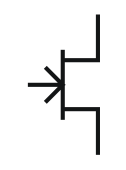
\includegraphics{njfetSymbol}}
{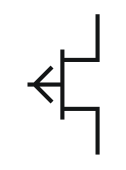
\includegraphics{pjfetSymbol}}

\device
J<name> <drain node> <gate node> <source node> <model name>
+ [area value] [device parameters]

\examples
\begin{alltt}
JIN 100 1 0 JFAST
J13 22 14 23 JNOM 2.0
J1 1 2 0 2N5114
\end{alltt}

\model
\begin{alltt}
.MODEL <model name> NJF [model parameters]
.MODEL <model name> PJF [model parameters]
\end{alltt}

\parameters

\begin{Parameters}

\param{drain node}
Node connected to drain.

\param{gate node}
Node connected to gate.

\param{source node}
 Node connected to source.

\param{source node}
Name of model defined in .MODEL line.

\param{area value}

The \texttt{JFET} is modeled as an intrinsic FET using an ohmic
resistance (\texttt{RD/area}) in series with the drain and another ohmic
resistance (\texttt{RS/area}) in series with the source.  \texttt{area}
is an area factor with a default of \texttt{1}.

\param{device parameters}

Parameters listed in Table~\ref{J_1_Device_Instance_Params} may be
provided as space separated \texttt{<parameter>=<value>} specifications
as needed.  Any number of parameters may be specified.

\end{Parameters}

\comments

The \texttt{JFET} was first proposed and analyzed by Shockley.  The
SPICE- compatible \texttt{JFET} model is an approximation to the
Shockley analysis that employs an adjustable parameter B.  Both the
Shockley formulation and the SPICE approximation are available in Xyce.

\end{Device}

\pagebreak

\paragraph{Device Parameters}
% This table was generated by Xyce:
%   Xyce -doc J 1
%
\index{jfet!device instance parameters}
\begin{DeviceParamTableGenerated}{JFET Device Instance Parameters}{J_1_Device_Instance_Params}
AREA & Device area & m$^{2}$ & 1 \\ \hline
TEMP & Device temperature & -- & Ambient Temperature \\ \hline
\end{DeviceParamTableGenerated}


\paragraph{Model Parameters}
% This table was generated by Xyce:
%   Xyce -doc J 1
%
\index{jfet!device model parameters}
\begin{DeviceParamTableGenerated}{JFET Device Model Parameters}{J_1_Device_Model_Params}
AF & Flicker noise exponent & -- & 1 \\ \hline
B & Doping tail parameter (level 1) & V$^{-1}$ & 1 \\ \hline
BETA & Transconductance parameter & A/V$^{2}$ & 0.0001 \\ \hline
CGD & Zero-bias gate-drain junction capacitance & F & 0 \\ \hline
CGS & Zero-bias gate-source junction capacitance & F & 0 \\ \hline
DELTA & Saturation voltage parrameter (level 2) & V & 0 \\ \hline
FC & Coefficient for forward-bias depletion capacitance & F & 0.5 \\ \hline
IS & Gate junction saturation current & A & 1e-14 \\ \hline
KF & Flicker noise coefficient & -- & 0.05 \\ \hline
LAMBDA & Channel length modulation & V$^{-1}$ & 0 \\ \hline
PB & Gate junction potential & V & 1 \\ \hline
RD & Drain ohmic resistance & $\mathsf{\Omega}$ & 0 \\ \hline
RS & Source ohmic resistance & $\mathsf{\Omega}$ & 0 \\ \hline
TEMPMODEL & Specifies the type of parameter interpolation over temperature & -- & 'NONE' \\ \hline
THETA & Mobility modulation parameter (level 2) & V$^{-1}$ & 0 \\ \hline
TNOM & Nominal device temperature & $^\circ$C & Ambient Temperature \\ \hline
VTO & Threshold voltage & V & -2 \\ \hline
\end{DeviceParamTableGenerated}


\pagebreak

\paragraph{Device Parameters}
% This table was generated by Xyce:
%   Xyce -doc J 2
%
\index{jfet!device instance parameters}
\begin{DeviceParamTableGenerated}{JFET Device Instance Parameters}{J_2_Device_Instance_Params}
AREA & Device area & m$^{2}$ & 1 \\ \hline
TEMP & Device temperature & -- & Ambient Temperature \\ \hline
\end{DeviceParamTableGenerated}


\paragraph{Model Parameters}
% This table was generated by Xyce:
%   Xyce -doc J 2
%
\index{jfet!device model parameters}
\begin{DeviceParamTableGenerated}{JFET Device Model Parameters}{J_2_Device_Model_Params}
AF & Flicker noise exponent & -- & 1 \\ \hline
B & Doping tail parameter (level 1) & V$^{-1}$ & 1 \\ \hline
BETA & Transconductance parameter & A/V$^{2}$ & 0.0001 \\ \hline
CGD & Zero-bias gate-drain junction capacitance & F & 0 \\ \hline
CGS & Zero-bias gate-source junction capacitance & F & 0 \\ \hline
DELTA & Saturation voltage parrameter (level 2) & V & 0 \\ \hline
FC & Coefficient for forward-bias depletion capacitance & F & 0.5 \\ \hline
IS & Gate junction saturation current & A & 1e-14 \\ \hline
KF & Flicker noise coefficient & -- & 0.05 \\ \hline
LAMBDA & Channel length modulation & V$^{-1}$ & 0 \\ \hline
PB & Gate junction potential & V & 1 \\ \hline
RD & Drain ohmic resistance & $\mathsf{\Omega}$ & 0 \\ \hline
RS & Source ohmic resistance & $\mathsf{\Omega}$ & 0 \\ \hline
TEMPMODEL & Specifies the type of parameter interpolation over temperature & -- & 'NONE' \\ \hline
THETA & Mobility modulation parameter (level 2) & V$^{-1}$ & 0 \\ \hline
TNOM & Nominal device temperature & $^\circ$C & Ambient Temperature \\ \hline
VTO & Threshold voltage & V & -2 \\ \hline
\end{DeviceParamTableGenerated}


\paragraph{JFET Level selection}
\Xyce{} supports two JFET models.  LEVEL=1, the default, is the SPICE 3f5
treatment.  This model employs a doping profile parameter B.  When B=1,
the original SPICE square law is exactly implemented, and when B=0.6 the
model is close to that of Shockley.

When LEVEL=2 is selected, the Shockley model is used with some additional physics
effects:  channel length modulation and the effect of gate electric field on
mobility.  An additional parameter, DELTA, is added to the LEVEL 2 model that
allows the user to adjust the saturation voltage.

\paragraph{JFET Power Calculations}
Power dissipated in the transistor is calculated with $I_{D}*V_{DS}+I_{G}*V_{GS}$ where
$I_{D}$ is the drain current, $I_{G}$ is the gate current, $V_{DS}$ is the 
voltage drop between the drain and the source and $V_{GS}$ is the voltage drop 
between the gate and the source. This formula may differ from other simulators,
such as HSPICE and PSpice.


%%
%% MESFET Section
%%
\clearpage
\subsection{Metal-Semiconductor FET (MESFET)}
\index{device!MESFET} \index{MESFET}
% Sandia National Laboratories is a multimission laboratory managed and
% operated by National Technology & Engineering Solutions of Sandia, LLC, a
% wholly owned subsidiary of Honeywell International Inc., for the U.S.
% Department of Energy’s National Nuclear Security Administration under
% contract DE-NA0003525.

% Copyright 2002-2022 National Technology & Engineering Solutions of Sandia,
% LLC (NTESS).


\begin{Device}\label{Z_DEVICE}

\symbol
{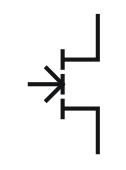
\includegraphics{nmesfetSymbol}}
{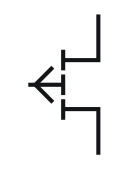
\includegraphics{pmesfetSymbol}}

\device
\begin{alltt}
Z<name> < drain node> <gate node> <source node> <model name>
+ [area value] [device parameters]
\end{alltt}

\model
\begin{alltt}
.MODEL <model name> NMF [model parameters]
.MODEL <model name> PMF [model parameters]
\end{alltt}

\examples
\begin{alltt}
Z1 2 3 0 MESMOD AREA=1.4
Z1 7 2 3 ZM1
\end{alltt}

\parameters

\begin{Parameters}

\param{drain node}
Node connected to drain.

\param{gate node}
Node connected to gate.

\param{source node}
Node connected to source.

\param{source node}
Name of model defined in .MODEL line.

\param{area value}

The \texttt{MESFET} is modeled as an intrinsic FET using an ohmic
resistance (\texttt{RD/area}) in series with the drain and another ohmic
resistance (\texttt{RS/area}) in series with the source.  \texttt{area value}
is a scaling factor with a default of 1.

\param{device parameters}

Parameters listed in Table~\ref{Z_1_Device_Instance_Params} may be
provided as space separated \texttt{<parameter>=<value>} specifications
as needed.  Any number of parameters may be specified.

\end{Parameters}

\comments

Although MESFETs can be made of Si, such devices are not as common as
GaAs MESFETS.  And since the mobility of electrons is much higher than
holes in GaAs, nearly all commercial devices are n-type MESFETS.

\end{Device}

\pagebreak

\paragraph{Device Parameters}
% This table was generated by Xyce:
%   Xyce -doc Z 1
%
\index{mesfet!device instance parameters}
\begin{DeviceParamTableGenerated}{MESFET Device Instance Parameters}{Z_1_Device_Instance_Params}
AREA & device area & m$^{2}$ & 1 \\ \hline
TEMP & Device temperature & -- & Ambient Temperature \\ \hline
\end{DeviceParamTableGenerated}


\paragraph{Model Parameters}
% This table was generated by Xyce:
%   Xyce -doc Z 1
%
\index{mesfet!device model parameters}
\begin{DeviceParamTableGenerated}{MESFET Device Model Parameters}{Z_1_Device_Model_Params}
AF & Flicker noise exponent & -- & 1 \\ \hline
ALPHA & Saturation voltage parameter & V$^{-1}$ & 2 \\ \hline
B & Doping tail parameter & V$^{-1}$ & 0.3 \\ \hline
BETA & Transconductance parameter & A/V$^{2}$ & 0.0025 \\ \hline
CGD & Zero-bias gate-drain junction capacitance & F & 0 \\ \hline
CGS & Zero-bias gate-source junction capacitance & F & 0 \\ \hline
FC & Coefficient for forward-bias depletion capacitance & F & 0.5 \\ \hline
IS & Gate junction saturation current & A & 1e-14 \\ \hline
KF & Flicker noise coefficient & -- & 0.05 \\ \hline
LAMBDA & Channel length modulation & V$^{-1}$ & 0 \\ \hline
PB & Gate junction potential & V & 1 \\ \hline
RD & Drain ohmic resistance & $\mathsf{\Omega}$ & 0 \\ \hline
RS & Source ohmic resistance & $\mathsf{\Omega}$ & 0 \\ \hline
TEMPMODEL & Specifies the type of parameter interpolation over temperature & -- & 'NONE' \\ \hline
TNOM & Nominal device temperature & $^\circ$C & Ambient Temperature \\ \hline
VTO & Threshold voltage & V & 0 \\ \hline
\end{DeviceParamTableGenerated}


\paragraph{MESFET Power Calculations}
Power dissipated in the transistor is calculated with $I_{D}*V_{DS}+I_{G}*V_{GS}$ where
$I_{D}$ is the drain current, $I_{G}$ is the gate current, $V_{DS}$ is the 
voltage drop between the drain and the source and $V_{GS}$ is the voltage drop 
between the gate and the source. This formula may differ from other simulators,
such as HSPICE and PSpice.


%%
%% MOSFET Subsection
%%
\clearpage
\subsection{MOS Field Effect Transistor (MOSFET)}
\index{device!MOSFET} \index{MOSFET}
% Sandia National Laboratories is a multimission laboratory managed and
% operated by National Technology & Engineering Solutions of Sandia, LLC, a
% wholly owned subsidiary of Honeywell International Inc., for the U.S.
% Department of Energy’s National Nuclear Security Administration under
% contract DE-NA0003525.

% Copyright 2002-2020 National Technology & Engineering Solutions of Sandia,
% LLC (NTESS).


\begin{Device}\label{M_DEVICE}

\symbol
{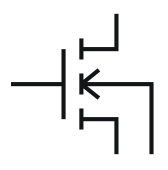
\includegraphics{nmosSymbol}}
{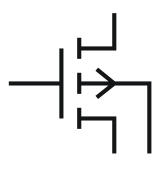
\includegraphics{pmosSymbol}}

\device
\begin{alltt}
M<name> <drain node> <gate node> <source node>
+ <bulk/substrate node> <model name>
+ [L=<value>] [W=<value>]
+ [AD=<value>] [AS=<value>]
+ [PD=<value>] [PS=<value>]
+ [NRD=<value>] [NRS=<value>]
+ [M=<value] [IC=<value, ...>]
\end{alltt}

\vbox{\hrulefill}
\item[Special Form (BSIMSOI)]
\begin{alltt}
M<name> <drain node> <gate node> <source node>
+ <substrate node (E)>
+ [<External body contact (P)>]
+ [<internal body contact (B)>]
+ [<temperature node (T)>]
+ <model name>
+ [L=<value>] [W=<value>]
+ [AD=<value>] [AS=<value>]
+ [PD=<value>] [PS=<value>]
+ [NRD=<value>] [NRS=<value>] [NRB=<value>]
+ [BJTOFF=<value>]
+ [IC=<val>,<val>,<val>,<val>,<val>]
+ [RTH0=<val>] [CTH0=<val>]
+ [NBC=<val>] [NSEG=<val>] [PDBCP=<val>] [PSBCP=<val>]
+ [AGBCP=<val>] [AEBCP=<val>] [VBSUSR=<val>] [TNODEOUT]
+ [FRBODY=<val>] [M=<value>]
\end{alltt}
\vbox{\hrulefill}

\item[Special Form (MVS)]
\begin{alltt}
M<name> <drain node> <gate node> <source node> <model name>
\end{alltt}

\item[Special Form (PSP103 with self-heating)]
\begin{alltt}
M<name> <drain node> <gate node> <source node> <bulk node> <dt node> <model name> [instance parameters]
\end{alltt}

\model
\begin{alltt}
.MODEL <model name> NMOS [model parameters]
.MODEL <model name> PMOS [model parameters]
\end{alltt}

\examples
\begin{alltt}
M5 4 12 3 0 PNOM L=20u W=10u
M3 5 13 10 0 PSTRONG
M6 7 13 10 0 PSTRONG M=2
M8 10 12 100 100 NWEAK L=30u W=20u
+ AD=288p AS=288p PD=60u PS=60u NRD=14 NRS=24
\end{alltt}

\parameters

\begin{Parameters}

\param{\vbox{\hbox{L\hfil}\hbox{M\hfil}}}

The MOSFET channel length and width that are decreased to get the actual
channel length and width. They may be given in the device
\texttt{.MODEL} or \texttt{.OPTIONS} statements. The value in the device
statement overrides the value in the model statement, which overrides
the value in the \texttt{.OPTIONS} statement. If \texttt{L} or \texttt{W}
values are not given, their default value is 100~$\mu$m.

\param{\vbox{\hbox{AD\hfil}\hbox{AS\hfil}}}

The drain and source diffusion areas. Defaults for \texttt{AD} and
\texttt{AS} can be set in the \texttt{.OPTIONS} statement.  If
\texttt{AD} or \texttt{AS} defaults are not set, their default value is
0.

\param{\vbox{\hbox{PD\hfil}\hbox{PS\hfil}}}
The drain and source diffusion perimeters. Their default value is 0.

\param{\vbox{\hbox{NRD\hfil}\hbox{NRS\hfil}}}

Multipliers (in units of $\Box$) that can be multiplied by \texttt{RSH}
to yield the parasitic (ohmic) resistances of the drain (\texttt{RD})
and source (\texttt{RS}), respectively.  \texttt{NRD}, \texttt{NRS}
default to 0.

Consider a square sheet of resistive material. Analysis shows that the
resistance between two parallel edges of such a sheet depends upon its
composition and thickness, but is independent of its size as long as it is
square. In other words, the resistance will be the same whether the square's
edge is 2~mm, 2~cm, or 2~m. For this reason, the \emph{sheet resistance} of
such a layer, abbreviated \texttt{RSH}, has units of Ohms per square,
written $\mathsf{\Omega}/\Box$.

\param{M}

If specified, the value is used as a number of parallel MOSFETs to be
simulated.  For example, if \texttt{M=2} is specified, \Xyce{} simulates two
identical mosfets connected to the same nodes in parallel.

\param{IC}

The BSIM3 (model level 9), BSIM4 (model level 14 or 54) and BSIMSOI (model
level 10) allow one to specify the initial voltage difference across
nodes of the device during the DC operating point calculation.  For the
BSIM3 and BSIM4 the syntax is \texttt{IC=$V_{ds}, V_{gs}, V_{bs}$}
where $V_{ds}$ is the voltage difference between the drain and source,
$V_{gs}$ is the voltage difference between the gate and source and
$V_{bs}$ is the voltage difference between the body and source.  The
BSIMSOI device's initial condition syntax is \texttt{IC=$V_{ds},
  V_{gs}, V_{bs}, V_{es}, V_{ps}$} where the two extra terms are the
voltage difference between the substrate and source, and the external
body and source nodes respectively.  Note that for any of these lists of
voltage differences, fewer than the full number of options may be
specified.  For example, \texttt{IC=5.0} specifies an initial condition on $V_{ds}$
but does not specifiy any initial conditions on the other nodes.
Therefore, one cannot specify $V_{gs}$ without specifying $V_{ds}$, etc.

It is illegal to specify initial conditions on any nodes that are tied
together.  \Xyce{} attempts to catch such errors, but complex circuits may
stymie this error trap.

\end{Parameters}

\vbox{\hrulefill}
\item[BSIMSOI Options]

There are a large number of extra instance parameters and optional
nodes available for the BSIMSOI (level 10) MOSFET.

\begin{Parameters}

\param{substrate node}

The fourth node of the BSIMSOI device is always the substrate node,
which is referred to as the \texttt{E} node. 

\param{external body contact node}

If given, the fifth node is the external body contact node,
\texttt{P}.  It is connected to the internal body node through a body
tie resistor.  If \texttt{P} is not given, the internal body node is
not accessible from the netlist and floats.

If there are only five nodes specified and \texttt{TNODEOUT} is also specified,
the fifth node is the temperature node instead.

\param{internal body contact node}

If given, the sixth node is the internal body contact node, \texttt{B}.  It is
connected to the external body node through a body tie resistor.  If \texttt{B}
is not given and \texttt{P} is given, the internal body node is not accessible
from the netlist, but is still tied to the external body contact through the
tie resistance.

If there are only six nodes specified and \texttt{TNODEOUT} is also specified,
the sixth node is the temperature node instead.

\param{temperature node}

If the parameter \texttt{TNODEOUT} is specified, the final node (fifth, sixth,
or seventh) is interpreted as a temperature node.  The temperature node is
intended for thermal coupling simulation.


\param{BJTOFF}
Turns off the parasitic BJT currents.

\param{IC}
The \texttt{IC} parameter allows specification of the five junction initial
conditions, $V_{ds}, V_{gs}, V_{bs}, V_{es}$ and $V_{ps}$.  $V_{ps}$ is ignored
in a four-terminal device.

\param{RTH0}
Thermal resistance per unit width.  Taken from model card if not given.

\param{CTH0}
Thermal capacitance per unit width.  Taken from model card if not given.

\param{NBC}
Number of body contact isolation edges.

\param{NSEG}
Number of segments for channel width partitioning.

\param{PDBCP}
Parasitic perimeter length for body contact at drain side.

\param{PSBCP}
Parasitic perimeter length for body contact at source side.

\param{AGBCP}
Parasitic gate-to-body overlap area for body contact.

\param{AEBCP}
Parasitic body-to-substrate overlap area for body contact.

\param{VBSUSR}
Optional initial value of VBS specified by user for use in transient
analysis.  (unused in \Xyce{}).

\param{FRBODY}
Layout-dependent body resistance coefficient.

\end{Parameters}

\comments

The simulator provides three MOSFET device models, which differ in the
formulation of the I-V characteristic. The \texttt{LEVEL} parameter
selects among different models as shown below.

For HSPICE compatibility, the BSIM4 model can be specified with either
level 14 or level 54.

\end{Device}

\paragraph{MOSFET Operating Temperature}
Model parameters may be assigned unique measurement temperatures using the
\textrmb{TNOM} model parameter. See the MOSFET model parameters for more
information.

\paragraph{MOSFET Power Calculations}
Power dissipated in the transistor is calculated with $I_{D}*V_{DS}+I_{G}*V_{GS}$ where
$I_{D}$ is the drain current, $I_{G}$ is the gate current, $V_{DS}$ is the
voltage drop between the drain and the source and $V_{GS}$ is the voltage drop
between the gate and the source. This formula may differ from other simulators,
such as HSPICE and PSpice.

\paragraph{Internal Device Variables Accessible with {\tt N()} Syntax}
For the BSIM3, BSIM4, and BSIM-CMG version 110 models, several
internal variables have been made accessible with the {\tt N()} syntax
on a {\tt .PRINT} line.  They are $g_{m}$ (tranconductance), $V_{th}$,
$V_{ds}$, $V_{gs}$, $V_{bs}$, and $V_{dsat}$.  An example {\tt .PRINT}
line command for a MOSFET device named {\tt m1} would be:
\begin{alltt}
.print dc N(m1:gm) N(m1:Vth) N(m1:Vdsat) N(m1:Vds) N(m1:Vgs) N(m1:Vbs)
\end{alltt}
The BSIM-CMG also supports output of $I_{ds}$ (drain-source current)
in this manner.

If the user runs \texttt{Xyce -namesfile <filename> <netlist>} then
\Xyce{} will output into the first filename a list of all solution
variables generated by that netlist. This can be useful for
determining the ``fully-qualified'' device name, needed for the {\tt
  N()} syntax, if the device is in a subcircuit.

\paragraph{Instance Parameters}
Tables ~\ref{M_1_Device_Instance_Params}, ~\ref{M_2_Device_Instance_Params}, 
~\ref{M_3_Device_Instance_Params},  ~\ref{M_6_Device_Instance_Params},
\ref{M_9_Device_Instance_Params} and \ref{M_10_Device_Instance_Params}  
give the available instance parameters for the levels 1,2,3,6,9 and 10 MOSFETs,
respectively.

In addition to the parameters shown in the tables, where a list of
numbered initial condition parameters are shown, the MOSFETs support a vector
parameter for the initial conditions.  \texttt{IC1} and \texttt{IC2}
may therefore be specified compactly as \texttt{IC=<ic1>,<ic2>}.

\paragraph{Model Parameters}
Tables ~\ref{M_1_Device_Model_Params}, ~\ref{M_2_Device_Model_Params},
~\ref{M_3_Device_Model_Params}, ~\ref{M_6_Device_Model_Params},
~\ref{M_9_Device_Model_Params}, and ~\ref{M_10_Device_Model_Params}
give the available model parameters for the levels 1,2,3,6,9 and 10 MOSFETs,
respectively.

For a thorough description of MOSFET models see~\cite{Antognetti:1988, HLJHCKH,
BLETK:1997, SH:1968, VL:1980,
SSKJ:1987, Pierret:1984, YEC:1983, BSIM3:V3:1, BN}.

\subparagraph{All MOSFET models}
The parameters shared by all MOSFET model levels are principally parasitic
element values (e.g., series resistance, overlap capacitance, etc.).

\subparagraph{Model levels 1 and 3}
The DC behaviors of the level 1 and 3 MOSFET models are defined by the
parameters \textrmb{VTO}, \textrmb{KP}, \textrmb{LAMBDA}, \textrmb{PHI}, and
\textrmb{GAMMA}.  The simulator calculates these if the process parameters
(e.g., \textrmb{TOX}, and \textrmb{NSUB}) are specified, but these are always
overridden by any user-defined values. The \textrmb{VTO} value is positive
(negative) for modeling the enhancement mode and negative (positive) for the
depletion mode of N-channel (P-channel) devices.

For MOSFETs, the capacitance model enforces charge conservation,
influencing just the Level 1 and 3 models.

Effective device parameter lengths and widths are calculated as follows:
\[
P_i = P_0 + P_L / L_e + P_W / W_e
\]
where
\[
\begin{array}{rclcl}
L_e & = & \mbox{effective length} & = & \mathbf{L} - (2 \cdot \mathbf{LD}) \\
W_e & = & \mbox{effective width} & = & \mathbf{W} - (2 \cdot \mathbf{WD})
\end{array}
\]

See \textrmb{.MODEL} (model definition) for more information.

\subparagraph{Model level 9 (BSIM3 version 3.2.2)}
The University of California, Berkeley BSIM3 model is a physical-based model
with a large number of dependencies on essential dimensional and processing
parameters.  It incorporates the key effects that are critical in modeling
deep-submicrometer MOSFETs.  These include threshold voltage reduction,
nonuniform doping, mobility reduction due to the vertical field, bulk charge
effect, carrier velocity saturation, drain-induced barrier lowering (DIBL),
channel length modulation (CLM), hot-carrier-induced output resistance
reduction, subthreshold conduction, source/drain parasitic resistance,
substrate current induced body effect (SCBE) and drain voltage reduction in LDD
structure.

The BSIM3 Version 3.2.2 model is a deep submicron MOSFET model with several major
enhancements over earlier versions.  These include a single I-V formula used
to define the current and output conductance for operating regions, improved
narrow width device modeling, a superior capacitance model with improved short
and narrow geometry models, a new relaxation-time model to better transient
modeling and enhanced model fitting of assorted W/L ratios using a single
parameter set.  This version preserves the large number of integrated
dependencies on dimensional and processing parameters of the Version 2 model.
For further information, see Reference~\cite{HLJHCKH}.

\subparagraph{Additional notes}
\begin{enumerate}
\item If any of the following BSIM3 3.2.2 model parameters are not specified,
they are computed via the following:

If \textrmb{VTHO} is not specified, then:
\[
\mathbf{VTHO} = \mathbf{VFB} + \phi_s \mathbf{K1} \sqrt{\phi_s}
\]
where:
\[
\mathbf{VFB} = -1.0
\]
If \textrmb{VTHO} is given, then:
\begin{eqnarray*}
\mathbf{VFB} & = & \mathbf{VTHO} - \phi_s + \mathbf{K1}\sqrt{phi_s} \\
\mathbf{VBX} & = & \phi_s - \frac{q\cdot\mathbf{NCH} \cdot
\mathbf{XT}^2}{2\varepsilon_{si}} \\
\mathbf{CF} & = & \left( \frac{2\varepsilon_{ox}}{\pi} \right)
\ln \left(1 + \frac{1}{4 \times 10^7\cdot\mathbf{TOX}} \right)
\end{eqnarray*}
where:
\[
E_g(T) = \mbox{the energy bandgap at temperature }T = 1.16 - \frac{T^2}{7.02
\times 10^4(T + 1108)}
\]

\item If \textrmb{K1} and \textrmb{K2} are not given then they are computed via
the following:
\begin{eqnarray*}
\mathbf{K1} &=& \mathbf{GAMMA2} - 2 \cdot \mathbf{K2} \sqrt{\phi_s -
\mathbf{VBM}} \\
\mathbf{K2} &=& \frac{(\mathbf{GAMMA1} -
\mathbf{GAMMA2})(\sqrt{\phi_s - \mathbf{VBX}} -
\sqrt{\phi_s})}{2\sqrt{\phi_s}(\sqrt{\phi_s - \mathbf{VBM}} -
\sqrt{\phi_s}) + \mathbf{VBM}}
\end{eqnarray*}
where:
\begin{eqnarray*}
\phi_s & = & 2V_t \ln \left(\frac{\mathbf{NCH}}{n_i} \right) \\
V_t    & = & kT / q \\
n_i    & = & 1.45 \times 10^{10} \left(\frac{T}{300.15}
\right)^{1.5} \exp \left(21.5565981 - \frac{E_g(T)}{2V_t} \right)
\end{eqnarray*}

\item If \textrmb{NCH} is not specified and \textrmb{GAMMA1} is, then:
\[
\mathbf{NCH} = \frac{\mathbf{GAMMA1^2 \times \mathbf{COX}^2}}
{2q \varepsilon_{si}}
\]
If \textrmb{GAMMA1} and \textrmb{NCH} {\em are not} specified, then
\textrmb{NCH} defaults to $1.7\times10^{23}\;m^{-3}$ and \textrmb{GAMMA1} is
computed using \textrmb{NCH}:
\[
\mathbf{GAMMA1} = \frac{\sqrt{2q\varepsilon_{si} \cdot \mathbf{NCH}}}
{\mathbf{COX}}
\]
If \textrmb{GAMMA2} is not specified, then:
\[
\mathbf{GAMMA2} = \frac{\sqrt{2q\varepsilon_{si} \cdot \mathbf{NSUB}}}
{\mathbf{COX}}
\]

\item If \textrmb{CGSO} is not specified and $\mathbf{DLC} > 0$, then:
\[
\mathbf{CGSO} = \left\{ \begin{array}{ll}
0, & ((\mathbf{DLC \cdot COX) - CGSL)} < 0        \\
0.6 \cdot \mathbf{XJ \cdot COX}, & ((\mathbf{DLC \cdot COX) - CGSL)}
\geq 0
\end{array}
\right.
\]

\item If \textrmb{CGDO} is not specified and $\mathbf{DLC} > 0$, then:
\[
\mathbf{CGDO} = \left\{ \begin{array}{ll}
0, & ((\mathbf{DLC \cdot COX) - CGSL)} < 0 \\
0.6 \cdot \mathbf{XJ \cdot COX},
& ((\mathbf{DLC \cdot COX) - CGSL)} \geq 0
\end{array}
\right. \]
\end{enumerate}

\subparagraph{Model level 10 (BSIMSOI version 3.2)}

The BSIMSOI is an international standard model for SOI (silicon on insulator)
circuit design and is formulated on top of the BSIM3v3 framework.
A detailed description can be found in the BSIMSOI 3.1 User's
Manual~\cite{BSIMSOI:Manual} and the BSIMSOI 3.2 release
notes~\cite{BSIMSOI:3p2:Notes}.

This version (v3.2) of the BSIMSOI includes three depletion models;
the partially depleted BSIMSOI PD (soiMod=0), the fully depleted BSIMSOI
FD (soiMod=2), and the unified SOI model (soiMod=1).

BSIMPD is the
Partial-Depletion (PD) mode of the BSIMSOI.  A typical PD SOI MOSFET is formed
on a thin SOI film which is layered on top of a buried oxide.  BSIMPD has
the following features and enhancements:
\begin{XyceItemize}
\item Real floating body simulation of both I-V and C-V.  The body potential is
      determined by the balance of all body current components.
\item An improved parasitic bipolar current model.  This includes enhancements in
      the various diode leakage components, second order effects (high-level
      injection and Early effect), diffusion charge equation, and temperature
      dependence of the diode junction capacitance.
\item An improved impact-ionization current model.  The contribution from BJT
      current is also modeled by the parameter Fbjtii.
\item A gate-to-body tunneling current model, which is important to thin-oxide
      SOI technologies.
\item Enhancements in the threshold voltage and bulk charge formulation of the
      high positive body bias regime.
\item Instance parameters (Pdbcp, Psbcp, Agbcp, Aebcp, Nbc) are provided to model
      the parasitics of devices with various body-contact and isolation structures.
\item An external body node (the 6th node) and other improvements are introduced
      to facilitate the modeling of distributed body resistance.
\item Self heating.  An external temperature node (the 7th node) is supported to
      facilitate the simulation of thermal coupling among neighboring devices.
\item A unique SOI low frequency noise model, including a new excess noise resulting
      from the floating body effect.
\item Width dependence of the body effect is modeled by parameters (K1,K1w1,K1w2).
\item Improved history dependence of the body charges with two new parameters
      (Fbody, DLCB).
\item An instance parameter Vbsusr is provided for users to set the transient initial
      condition of the body potential.
\item The new charge-thickness capacitance model introduced in BSIM3v3.2,
      \texttt{capMod=3}, is included.
\end{XyceItemize}

\paragraph{Quadratic Temperature Compensation}
SPICE temperature effects are the default, but MOSFET levels 18, 19 and 20 have
a more advanced temperature compensation available.  By specifying
\texttt{TEMPMODEL=QUADRATIC} in the netlist, parameters can be interpolated
quadratically between measured values extracted from data.  See
Section~\ref{Model_Interpolation} for more details.

\paragraph{MOSFET Equations}
The following equations define an N-channel MOSFET. The P-channel
devices use a reverse the sign for all voltages and currents.  The
equations use the following variables:
\begin{eqnarray*}
V_{bs}  &=&\mbox{intrinsic substrate-intrinsic source voltage} \\
V_{bd}  &=&\mbox{intrinsic substrate-intrinsic drain voltage} \\
V_{ds}  &=&\mbox{intrinsic drain-substrate source voltage} \\
V_{dsat}&=&\mbox{saturation voltage} \\
V_{gs}  &=&\mbox{intrinsic gate-intrinsic source voltage} \\
V_{gd}  &=&\mbox{intrinsic gate-intrinsic drain voltage} \\
V_t     &=&kT / q \mbox{ (thermal voltage)} \\
V_{th}  &=&\mbox{threshold voltage} \\
C_{ox}  &=&\mbox{the gate oxide capacitance per unit area} \\
f       &=&\mbox{noise frequency} \\
k       &=&\mbox{Boltzmann's constant} \\
q       &=&\mbox{electron charge} \\
Leff    &=&\mbox{effective channel length} \\
Weff    &=&\mbox{effective channel width} \\
T       &=&\mbox{analysis temperature (K)} \\
T_0     &=&\mbox{nominal temperature (set using TNOM option)}
\end{eqnarray*}
Other variables are listed in the BJT Equations section~\ref{bjt_equations}.

\clearpage
\LTXtable{\textwidth}{mosfeteqntbl}

%%
%% MOSFET Equation Capacitance Table
%%
\paragraph{Capacitance}
\LTXtable{\textwidth}{mosfeteqncaptbl}

%%
%% MOSFET Equation Temperature Effects
%%
\clearpage
\paragraph{Temperature Effects}
\LTXtable{\textwidth}{mosfeteqntemptbl}

%%
%% MOSFET Parameters Table
%%
\clearpage
\subsubsection{Level 1 MOSFET Tables (SPICE Level 1)}
% This table was generated by Xyce:
%   Xyce -doc M 1
%
\index{mosfet level 1!device instance parameters}
\begin{DeviceParamTableGenerated}{MOSFET level 1 Device Instance Parameters}{M_1_Device_Instance_Params}
AD & Drain diffusion area & m$^{2}$ & 0 \\ \hline
AS & Source diffusion area & m$^{2}$ & 0 \\ \hline
IC1 & Initial condition on Drain-Source voltage & V & 0 \\ \hline
IC2 & Initial condition on Gate-Source voltage & V & 0 \\ \hline
IC3 & Initial condition on Bulk-Source voltage & V & 0 \\ \hline
L & Channel length & m & 0 \\ \hline
M & Multiplier for M devices connected in parallel & -- & 1 \\ \hline
NRD & Multiplier for RSH to yield parasitic resistance of drain & $\Box$ & 1 \\ \hline
NRS & Multiplier for RSH to yield parasitic resistance of source & $\Box$ & 1 \\ \hline
OFF & Initial condition of no voltage drops across device & logical (T/F) & false \\ \hline
PD & Drain diffusion perimeter & m & 0 \\ \hline
PS & Source diffusion perimeter & m & 0 \\ \hline
TEMP & Device temperature & $^\circ$C & Ambient Temperature \\ \hline
W & Channel width & m & 0 \\ \hline
\end{DeviceParamTableGenerated}

% This table was generated by Xyce:
%   Xyce -doc M 1
%
\index{mosfet level 1!device model parameters}
\begin{DeviceParamTableGenerated}{MOSFET level 1 Device Model Parameters}{M_1_Device_Model_Params}
AF & Flicker noise exponent & -- & 1 \\ \hline
CBD & Zero-bias bulk-drain p-n capacitance & F & 0 \\ \hline
CBS & Zero-bias bulk-source p-n capacitance & F & 0 \\ \hline
CGBO & Gate-bulk overlap capacitance/channel length & F/m & 0 \\ \hline
CGDO & Gate-drain overlap capacitance/channel width & F/m & 0 \\ \hline
CGSO & Gate-source overlap capacitance/channel width & F/m & 0 \\ \hline
CJ & Bulk p-n zero-bias bottom capacitance/area & F/m$^{2}$ & 0 \\ \hline
CJSW & Bulk p-n zero-bias sidewall capacitance/area & F/m$^{2}$ & 0 \\ \hline
FC & Bulk p-n forward-bias capacitance coefficient & -- & 0.5 \\ \hline
GAMMA & Bulk threshold parameter & V$^{1/2}$ & 0 \\ \hline
IS & Bulk p-n saturation current & A & 1e-14 \\ \hline
JS & Bulk p-n saturation current density & A/m$^{2}$ & 0 \\ \hline
KF & Flicker noise coefficient & -- & 0 \\ \hline
KP & Transconductance coefficient & A/V$^{2}$ & 2e-05 \\ \hline
L & Default channel length & m & 0.0001 \\ \hline
LAMBDA & Channel-length modulation & V$^{-1}$ & 0 \\ \hline
LD & Lateral diffusion length & m & 0 \\ \hline
MJ & Bulk p-n bottom grading coefficient & -- & 0.5 \\ \hline
MJSW & Bulk p-n sidewall grading coefficient & -- & 0.5 \\ \hline
NSS & Surface state density & cm$^{-2}$ & 0 \\ \hline
NSUB & Substrate doping density & cm$^{-3}$ & 0 \\ \hline
PB & Bulk p-n bottom potential & V & 0.8 \\ \hline
PHI & Surface potential & V & 0.6 \\ \hline
RD & Drain ohmic resistance & $\mathsf{\Omega}$ & 0 \\ \hline
RS & Source ohmic resistance & $\mathsf{\Omega}$ & 0 \\ \hline
RSH & Drain,source diffusion sheet resistance & $\mathsf{\Omega}$ & 0 \\ \hline
TEMPMODEL & Specifies the type of parameter interpolation over temperature & -- & 'NONE' \\ \hline
TNOM & Nominal device temperature & $^\circ$C & 27 \\ \hline
TOX & Gate oxide thickness & m & 1e-07 \\ \hline
TPG & Gate material type (-1 = same as substrate) 0 = aluminum,1 = opposite of substrate) & -- & 0 \\ \hline
U0 & Surface mobility & 1/(Vcm$^{2}$s) & 600 \\ \hline
UO & Surface mobility & 1/(Vcm$^{2}$s) & 600 \\ \hline
VTO & Zero-bias threshold voltage & V & 0 \\ \hline
W & Default channel width & m & 0.0001 \\ \hline
\end{DeviceParamTableGenerated}

\clearpage
\subsubsection{Level 2 MOSFET Tables (SPICE Level 2)}
% This table was generated by Xyce:
%   Xyce -doc M 2
%
\index{mosfet level 2!device instance parameters}
\begin{DeviceParamTableGenerated}{MOSFET level 2 Device Instance Parameters}{M_2_Device_Instance_Params}
AD & Drain diffusion area & m$^{2}$ & 0 \\ \hline
AS & Source diffusion area & m$^{2}$ & 0 \\ \hline
IC1 & Initial condition on Drain-Source voltage & V & 0 \\ \hline
IC2 & Initial condition on Gate-Source voltage & V & 0 \\ \hline
IC3 & Initial condition on Bulk-Source voltage & V & 0 \\ \hline
L & Channel length & m & 0 \\ \hline
M & Multiplier for M devices connected in parallel & -- & 1 \\ \hline
NRD & Multiplier for RSH to yield parasitic resistance of drain & $\Box$ & 1 \\ \hline
NRS & Multiplier for RSH to yield parasitic resistance of source & $\Box$ & 1 \\ \hline
OFF & Initial condition of no voltage drops across device & logical (T/F) & false \\ \hline
PD & Drain diffusion perimeter & m & 0 \\ \hline
PS & Source diffusion perimeter & m & 0 \\ \hline
TEMP & Device temperature & $^\circ$C & Ambient Temperature \\ \hline
W & Channel width & m & 0 \\ \hline
\end{DeviceParamTableGenerated}

% This table was generated by Xyce:
%   Xyce -doc M 2
%
\index{mosfet level 2!device model parameters}
\begin{DeviceParamTableGenerated}{MOSFET level 2 Device Model Parameters}{M_2_Device_Model_Params}
AF & Flicker noise exponent & -- & 1 \\ \hline
CBD & Zero-bias bulk-drain p-n capacitance & F & 0 \\ \hline
CBS & Zero-bias bulk-source p-n capacitance & F & 0 \\ \hline
CGBO & Gate-bulk overlap capacitance/channel length & F/m & 0 \\ \hline
CGDO & Gate-drain overlap capacitance/channel width & F/m & 0 \\ \hline
CGSO & Gate-source overlap capacitance/channel width & F/m & 0 \\ \hline
CJ & Bulk p-n zero-bias bottom capacitance/area & F/m$^{2}$ & 0 \\ \hline
CJSW & Bulk p-n zero-bias sidewall capacitance/area & F/m$^{2}$ & 0 \\ \hline
DELTA & Width effect on threshold & -- & 0 \\ \hline
FC & Bulk p-n forward-bias capacitance coefficient & -- & 0.5 \\ \hline
GAMMA & Bulk threshold parameter & V$^{1/2}$ & 0 \\ \hline
IS & Bulk p-n saturation current & A & 1e-14 \\ \hline
JS & Bulk p-n saturation current density & A/m$^{2}$ & 0 \\ \hline
KF & Flicker noise coefficient & -- & 0 \\ \hline
KP & Transconductance coefficient & A/V$^{2}$ & 2e-05 \\ \hline
L & Default channel length & m & 0.0001 \\ \hline
LAMBDA & Channel-length modulation & V$^{-1}$ & 0 \\ \hline
LD & Lateral diffusion length & m & 0 \\ \hline
MJ & Bulk p-n bottom grading coefficient & -- & 0.5 \\ \hline
MJSW & Bulk p-n sidewall grading coefficient & -- & 0.5 \\ \hline
NEFF & Total channel charge coeff. & -- & 1 \\ \hline
NFS & Fast surface state density & -- & 0 \\ \hline
NSS & Surface state density & cm$^{-2}$ & 0 \\ \hline
NSUB & Substrate doping density & cm$^{-3}$ & 0 \\ \hline
PB & Bulk p-n bottom potential & V & 0.8 \\ \hline
PHI & Surface potential & V & 0.6 \\ \hline
RD & Drain ohmic resistance & $\mathsf{\Omega}$ & 0 \\ \hline
RS & Source ohmic resistance & $\mathsf{\Omega}$ & 0 \\ \hline
RSH & Drain,source diffusion sheet resistance & $\mathsf{\Omega}$ & 0 \\ \hline
TEMPMODEL & Specifies the type of parameter interpolation over temperature & -- & 'NONE' \\ \hline
TNOM & Nominal device temperature & $^\circ$C & 27 \\ \hline
TOX & Gate oxide thickness & m & 1e-07 \\ \hline
TPG & Gate material type (-1 = same as substrate, 0 = aluminum,1 = opposite of substrate) & -- & 0 \\ \hline
U0 & Surface mobility & 1/(Vcm$^{2}$s) & 600 \\ \hline
UCRIT & Crit. field for mob. degradation & -- & 10000 \\ \hline
UEXP & Crit. field exp for mob. deg. & -- & 0 \\ \hline
UO & Surface mobility & 1/(Vcm$^{2}$s) & 600 \\ \hline
VMAX & Maximum carrier drift velocity & -- & 0 \\ \hline
VTO & Zero-bias threshold voltage & V & 0 \\ \hline
W & Default channel width & m & 0.0001 \\ \hline
XJ & Junction depth & -- & 0 \\ \hline
\end{DeviceParamTableGenerated}

\clearpage
\subsubsection{Level 3 MOSFET Tables (SPICE Level 3)}
% This table was generated by Xyce:
%   Xyce -doc M 3
%
\index{mosfet level 3!device instance parameters}
\begin{DeviceParamTableGenerated}{MOSFET level 3 Device Instance Parameters}{M_3_Device_Instance_Params}
AD & Drain diffusion area & m$^{2}$ & 0 \\ \hline
AS & Source diffusion area & m$^{2}$ & 0 \\ \hline
IC1 & Initial condition on Drain-Source voltage & V & 0 \\ \hline
IC2 & Initial condition on Gate-Source voltage & V & 0 \\ \hline
IC3 & Initial condition on Bulk-Source voltage & V & 0 \\ \hline
L & Channel length & m & 0 \\ \hline
M & Multiplier for M devices connected in parallel & -- & 1 \\ \hline
NRD & Multiplier for RSH to yield parasitic resistance of drain & $\Box$ & 1 \\ \hline
NRS & Multiplier for RSH to yield parasitic resistance of source & $\Box$ & 1 \\ \hline
OFF & Initial condition of no voltage drops across device & logical (T/F) & false \\ \hline
PD & Drain diffusion perimeter & m & 0 \\ \hline
PS & Source diffusion perimeter & m & 0 \\ \hline
TEMP & Device temperature & $^\circ$C & Ambient Temperature \\ \hline
W & Channel width & m & 0 \\ \hline
\end{DeviceParamTableGenerated}

% This table was generated by Xyce:
%   Xyce -doc M 3
%
\index{mosfet level 3!device model parameters}
\begin{DeviceParamTableGenerated}{MOSFET level 3 Device Model Parameters}{M_3_Device_Model_Params}
AF & Flicker noise exponent & -- & 1 \\ \hline
CBD & Zero-bias bulk-drain p-n capacitance & F & 0 \\ \hline
CBS & Zero-bias bulk-source p-n capacitance & F & 0 \\ \hline
CGBO & Gate-bulk overlap capacitance/channel length & F/m & 0 \\ \hline
CGDO & Gate-drain overlap capacitance/channel width & F/m & 0 \\ \hline
CGSO & Gate-source overlap capacitance/channel width & F/m & 0 \\ \hline
CJ & Bulk p-n zero-bias bottom capacitance/area & F/m$^{2}$ & 0 \\ \hline
CJSW & Bulk p-n zero-bias sidewall capacitance/area & F/m$^{2}$ & 0 \\ \hline
DELTA & Width effect on threshold & -- & 0 \\ \hline
ETA & Static feedback & -- & 0 \\ \hline
FC & Bulk p-n forward-bias capacitance coefficient & -- & 0.5 \\ \hline
GAMMA & Bulk threshold parameter & V$^{1/2}$ & 0 \\ \hline
IS & Bulk p-n saturation current & A & 1e-14 \\ \hline
JS & Bulk p-n saturation current density & A/m$^{2}$ & 0 \\ \hline
KAPPA & Saturation field factor & -- & 0.2 \\ \hline
KF & Flicker noise coefficient & -- & 0 \\ \hline
KP & Transconductance coefficient & A/V$^{2}$ & 2e-05 \\ \hline
L & Default channel length & m & 0.0001 \\ \hline
LD & Lateral diffusion length & m & 0 \\ \hline
MJ & Bulk p-n bottom grading coefficient & -- & 0.5 \\ \hline
MJSW & Bulk p-n sidewall grading coefficient & -- & 0.33 \\ \hline
NFS & Fast surface state density & cm$^{-2}$ & 0 \\ \hline
NSS & Surface state density & cm$^{-2}$ & 0 \\ \hline
NSUB & Substrate doping density & cm$^{-3}$ & 0 \\ \hline
PB & Bulk p-n bottom potential & V & 0.8 \\ \hline
PHI & Surface potential & V & 0.6 \\ \hline
RD & Drain ohmic resistance & $\mathsf{\Omega}$ & 0 \\ \hline
RS & Source ohmic resistance & $\mathsf{\Omega}$ & 0 \\ \hline
RSH & Drain,source diffusion sheet resistance & $\mathsf{\Omega}$ & 0 \\ \hline
TEMPMODEL & Specifies the type of parameter interpolation over temperature & -- & 'NONE' \\ \hline
THETA & Mobility modulation & V$^{-1}$ & 0 \\ \hline
TNOM & Nominal device temperature & $^\circ$C & 27 \\ \hline
TOX & Gate oxide thickness & m & 1e-07 \\ \hline
TPG & Gate material type (-1 = same as substrate,0 = aluminum,1 = opposite of substrate) & -- & 1 \\ \hline
U0 & Surface mobility & 1/(Vcm$^{2}$s) & 600 \\ \hline
UO & Surface mobility & 1/(Vcm$^{2}$s) & 600 \\ \hline
VMAX & Maximum drift velocity & m/s & 0 \\ \hline
VTO & Zero-bias threshold voltage & V & 0 \\ \hline
W & Default channel width & m & 0.0001 \\ \hline
XJ & Metallurgical junction depth & m & 0 \\ \hline
\end{DeviceParamTableGenerated}

\clearpage
\subsubsection{Level 6 MOSFET Tables (SPICE Level 6)}
% This table was generated by Xyce:
%   Xyce -doc M 6
%
\index{mosfet level 6!device instance parameters}
\begin{DeviceParamTableGenerated}{MOSFET level 6 Device Instance Parameters}{M_6_Device_Instance_Params}
AD & Drain diffusion area & m$^{2}$ & 0 \\ \hline
AS & Source diffusion area & m$^{2}$ & 0 \\ \hline
IC1 & Initial condition on Drain-Source voltage & V & 0 \\ \hline
IC2 & Initial condition on Gate-Source voltage & V & 0 \\ \hline
IC3 & Initial condition on Bulk-Source voltage & V & 0 \\ \hline
L & Channel length & m & 0 \\ \hline
M & Multiplier for M devices connected in parallel & -- & 1 \\ \hline
NRD & Multiplier for RSH to yield parasitic resistance of drain & $\Box$ & 1 \\ \hline
NRS & Multiplier for RSH to yield parasitic resistance of source & $\Box$ & 1 \\ \hline
OFF & Initial condition of no voltage drops across device & logical (T/F) & false \\ \hline
PD & Drain diffusion perimeter & m & 0 \\ \hline
PS & Source diffusion perimeter & m & 0 \\ \hline
TEMP & Device temperature & $^\circ$C & Ambient Temperature \\ \hline
W & Channel width & m & 0 \\ \hline
\end{DeviceParamTableGenerated}

% This table was generated by Xyce:
%   Xyce -doc M 6
%
\index{mosfet level 6!device model parameters}
\begin{DeviceParamTableGenerated}{MOSFET level 6 Device Model Parameters}{M_6_Device_Model_Params}
AF & Flicker noise exponent & -- & 1 \\ \hline
CBD & Zero-bias bulk-drain p-n capacitance & F & 0 \\ \hline
CBS & Zero-bias bulk-source p-n capacitance & F & 0 \\ \hline
CGBO & Gate-bulk overlap capacitance/channel length & F/m & 0 \\ \hline
CGDO & Gate-drain overlap capacitance/channel width & F/m & 0 \\ \hline
CGSO & Gate-source overlap capacitance/channel width & F/m & 0 \\ \hline
CJ & Bulk p-n zero-bias bottom capacitance/area & F/m$^{2}$ & 0 \\ \hline
CJSW & Bulk p-n zero-bias sidewall capacitance/area & F/m$^{2}$ & 0 \\ \hline
FC & Bulk p-n forward-bias capacitance coefficient & -- & 0.5 \\ \hline
GAMMA & Bulk threshold parameter & -- & 0 \\ \hline
GAMMA1 & Bulk threshold parameter 1 & -- & 0 \\ \hline
IS & Bulk p-n saturation current & A & 1e-14 \\ \hline
JS & Bulk p-n saturation current density & A/m$^{2}$ & 0 \\ \hline
KC & Saturation current factor & -- & 5e-05 \\ \hline
KF & Flicker noise coefficient & -- & 0 \\ \hline
KV & Saturation voltage factor & -- & 2 \\ \hline
LAMBDA & Channel length modulation param. & -- & 0 \\ \hline
LAMBDA0 & Channel length modulation param. 0 & -- & 0 \\ \hline
LAMBDA1 & Channel length modulation param. 1 & -- & 0 \\ \hline
LD & Lateral diffusion length & m & 0 \\ \hline
MJ & Bulk p-n bottom grading coefficient & -- & 0.5 \\ \hline
MJSW & Bulk p-n sidewall grading coefficient & -- & 0.5 \\ \hline
NC & Saturation current coeff. & -- & 1 \\ \hline
NSS & Surface state density & cm$^{-2}$ & 0 \\ \hline
NSUB & Substrate doping density & cm$^{-3}$ & 0 \\ \hline
NV & Saturation voltage coeff. & -- & 0.5 \\ \hline
NVTH & Threshold voltage coeff. & -- & 0.5 \\ \hline
PB & Bulk p-n bottom potential & V & 0.8 \\ \hline
PHI & Surface potential & V & 0.6 \\ \hline
PS & Sat. current modification  par. & -- & 0 \\ \hline
RD & Drain ohmic resistance & $\mathsf{\Omega}$ & 0 \\ \hline
RS & Source ohmic resistance & $\mathsf{\Omega}$ & 0 \\ \hline
RSH & Drain,source diffusion sheet resistance & $\mathsf{\Omega}$ & 0 \\ \hline
SIGMA & Static feedback effect par. & -- & 0 \\ \hline
TEMPMODEL & Specifies the type of parameter interpolation over temperature & -- & 'NONE' \\ \hline
TNOM & Nominal device temperature & $^\circ$C & 27 \\ \hline
TOX & Gate oxide thickness & m & 1e-07 \\ \hline
TPG & Gate material type (-1 = same as substrate,0 = aluminum,1 = opposite of substrate) & -- & 1 \\ \hline
U0 & Surface mobility & 1/(Vcm$^{2}$s) & 600 \\ \hline
UO & Surface mobility & 1/(Vcm$^{2}$s) & 600 \\ \hline
VTO & Zero-bias threshold voltage & V & 0 \\ \hline
\end{DeviceParamTableGenerated}

\clearpage
\subsubsection{Level 9 MOSFET Tables (BSIM3)}
For complete documentation of the BSIM3 model, see the users' manual for
the BSIM3, available for download at
\url{http://bsim.berkeley.edu/models/bsim4/bsim3/}.
\Xyce{} implements Version 3.2.2 of the BSIM3.

In addition to the parameters shown in
table~\ref{M_9_Device_Instance_Params}, the BSIM3 supports a vector
parameter for the initial conditions.  \texttt{IC1} through
\texttt{IC3} may therefore be specified compactly as
\texttt{IC=<ic1>,<ic2>,<ic3>}.

\textbf{NOTE:  Many BSIM3 parameters listed in
tables~\ref{M_9_Device_Instance_Params} and \ref{M_9_Device_Model_Params} as
having default values of zero are actually replaced with internally computed
defaults if not given.  Specifying zero in your model card will override this
internal computation.  It is recommended that you only set model parameters
that you are actually changing from defaults and that you not generate model
cards containing default values from the tables.}
% This table was generated by Xyce:
%   Xyce -doc_cat M 9
%
\index{bsim3!device instance parameters}
\begin{DeviceParamTableGenerated}{BSIM3 Device Instance Parameters}{M_9_Device_Instance_Params}

\category{Control Parameters}\\ \hline
M & Multiplier for M devices connected in parallel & -- & 1 \\ \hline
NQSMOD & Flag for NQS model & -- & 0 \\ \hline

\category{Geometry Parameters}\\ \hline
AD & Drain diffusion area & m$^{2}$ & 0 \\ \hline
AS & Source diffusion area & m$^{2}$ & 0 \\ \hline
L & Channel length & m & 0 \\ \hline
NRD & Multiplier for RSH to yield parasitic resistance of drain & $\Box$ & 1 \\ \hline
NRS & Multiplier for RSH to yield parasitic resistance of source & $\Box$ & 1 \\ \hline
PD & Drain diffusion perimeter & m & 0 \\ \hline
PS & Source diffusion perimeter & m & 0 \\ \hline
W & Channel width & m & 0 \\ \hline

\category{Temperature Parameters}\\ \hline
TEMP & Device temperature & $^\circ$C & Ambient Temperature \\ \hline

\category{Voltage Parameters}\\ \hline
IC1 & Initial condition on Vds & V & 0 \\ \hline
IC2 & Initial condition on Vgs & V & 0 \\ \hline
IC3 & Initial condition on Vbs & V & 0 \\ \hline
OFF & Initial condition of no voltage drops accross device & logical (T/F) & false \\ \hline
\end{DeviceParamTableGenerated}

% This table was generated by Xyce:
%   Xyce -doc_cat M 9
%
\index{bsim3!device model parameters}
\begin{DeviceParamTableGenerated}{BSIM3 Device Model Parameters}{M_9_Device_Model_Params}

\category{Bin Parameters}\\ \hline
LMAX & Maximum channel length & m & 1 \\ \hline
LMIN & Minimum channel length & m & 0 \\ \hline
WMAX & Maximum channel width & m & 1 \\ \hline
WMIN & Minimum channel width & m & 0 \\ \hline

\category{Capacitance Parameters}\\ \hline
ACDE & Exponetial coefficient for charge thickness in capmod = 3 for accumulation and depletion regions & m/V & 1 \\ \hline
CF & Firing field capacitance & F/m & 0 \\ \hline
CGBO & Gate-bulk overlap capacitance per unit channel length & F/m & 0 \\ \hline
CGDL & Light-doped drain-gate region overlap capacitance & F/m & 0 \\ \hline
CGDO & Non-LLD region drain-gate overlap capacitance per unit channel length & F/m & 0 \\ \hline
CGSL & Light-doped source-gate region overlap capacitance & F/m & 0 \\ \hline
CGSO & Non-LLD region source-gate overlap capacitance per unit channel length & F/m & 0 \\ \hline
CJ & Bulk p-n zero-bias bottom capacitance/area & F/m$^{2}$ & 0.0005 \\ \hline
CJSW & Bulk p-n zero-bias sidewall capacitance/area & F/m$^{2}$ & 5e-10 \\ \hline
CJSWG & Source/grain gate sidewall junction capacitance per unit width & F/m & 0 \\ \hline
CKAPPA & Coefficient for lightly doped region overlap capacitance fireing field capacitance & F/m & 0.6 \\ \hline
CLC & Constant term for short-channel model & m & 1e-07 \\ \hline
CLE & Exponetial term for the short-channel model & -- & 0.6 \\ \hline
DLC & Length offset fitting parameter from C-V & m & 0 \\ \hline
DWC & Width offset fitting parameter from C-V & m & 0 \\ \hline
MJSWG & Source/grain gate sidewall junction capacitance grading coeficient & -- & 0 \\ \hline
MOIN & Coefficient for the gate-bias dependent surface potential & -- & 15 \\ \hline
NOFF & CV parameter in Vgsteff,CV for weak to strong inversion & -- & 1 \\ \hline
PBSW & Source/drain side junction built-in potential & V & 1 \\ \hline
PBSWG & Source/drain gate sidewall junction built-in potential & V & 0 \\ \hline
VFBCV & Flat-band voltage parameter (for CAPMOD = 0 only) & V & -1 \\ \hline
VOFFCV & CV parameter in Vgsteff,CV for weak to strong inversion & V & 0 \\ \hline
XPART & Charge partitioning rate flag & -- & 0 \\ \hline

\category{Control Parameters}\\ \hline
BINUNIT & Binning unit selector & -- & 1 \\ \hline
CAPMOD & Flag for capacitance models & -- & 3 \\ \hline
MOBMOD & Mobility model selector & -- & 1 \\ \hline
NOIMOD & Flag for noise models & -- & 1 \\ \hline
PARAMCHK & Parameter value check & -- & 0 \\ \hline
VERSION & Version number & -- & '3.2.2' \\ \hline

\category{DC Parameters}\\ \hline
A0 & Bulk charge effect coefficient for channel length & -- & 1 \\ \hline
A1 & First non-saturation effect parameter & V$^{-1}$ & 0 \\ \hline
A2 & Second non-saturation factor & -- & 1 \\ \hline
AGS & Gate-bias coefficient of abulk & V$^{-1}$ & 0 \\ \hline
ALPHA0 & First parameter of impact-ionization current & m/V & 0 \\ \hline
ALPHA1 & Isub parameter for length scaling & V$^{-1}$ & 0 \\ \hline
B0 & Bulk charge effect coefficient for channel width & m & 0 \\ \hline
B1 & Bulk charge effect offset & m & 0 \\ \hline
BETA0 & Second parameter of impact-ionization current & V & 30 \\ \hline
CDSC & Drain/source to channel coupling capacitance & F/m$^{2}$ & 0.00024 \\ \hline
CDSCB & Body-bias sensitivity of CDSC & F/(Vm$^{2}$) & 0 \\ \hline
CDSCD & Drain-bias sensitivity of CDSC & F/(Vm$^{2}$) & 0 \\ \hline
CIT & Interface trap capacitance & F/m$^{2}$ & 0 \\ \hline
DELTA & Effective Vds parameter & V & 0.01 \\ \hline
DROUT & L-depedance Coefficient of the DIBL correction parameter in Rout & -- & 0.56 \\ \hline
DSUB & DIBL coefficient exponent in subthreshhold region & -- & 0 \\ \hline
DVT0 & First coefficient of short-channel effect effect on threshold voltage & -- & 2.2 \\ \hline
DVT0W & First coefficient of narrow-width effect effect on threshold voltage for small channel length & m$^{-1}$ & 0 \\ \hline
DVT1 & Second coefficient of short-channel effect effect on threshold voltage & -- & 0.53 \\ \hline
DVT1W & Second coefficient of narrow-width effect effect on threshold voltage for small channel length & m$^{-1}$ & 5.3e+06 \\ \hline
DVT2 & Body-bias coefficient of short-channel effect effect on threshold voltage & V$^{-1}$ & -0.032 \\ \hline
DVT2W & Body-bias coefficient of narrow-width effect effect on threshold voltage for small channel length & V$^{-1}$ & -0.032 \\ \hline
DWB & Coefficient of substrate body bias dependence of Weff & m/V$^{1/2}$ & 0 \\ \hline
DWG & Coefficient of gate depedence of Weff & m/V$^{1/2}$ & 0 \\ \hline
ETA0 & DIBL coefficient in subthreshold region & -- & 0.08 \\ \hline
ETAB & Body-bias coefficient for the subthreshold DIBL effect & V$^{-1}$ & -0.07 \\ \hline
IJTH & Diode limiting current & A & 0.1 \\ \hline
JSW & Sidewall saturation current per unit length & A/m & 0 \\ \hline
K1 & First-order body effect coefficient & V$^{1/2}$ & 0 \\ \hline
K2 & second-order body effect coefficient & -- & 0 \\ \hline
K3 & Narrow width coefficient & -- & 80 \\ \hline
K3B & Body effect coefficient of K3 & V$^{-1}$ & 0 \\ \hline
KETA & Body-bias coefficient of bulk charge effect & V$^{-1}$ & -0.047 \\ \hline
LINT & Length of offset fiting parameter from I-V without bias & m & 0 \\ \hline
LINTNOI & lint offset for noise calculation & m & 0 \\ \hline
NFACTOR & Subthreshold swing factor & -- & 1 \\ \hline
NGATE & Poly gate doping concentration & cm$^{-3}$ & 0 \\ \hline
NLX & Lateral non-uniform doping parameter & m & 1.74e-07 \\ \hline
PCLM & Channel length modulation parameter & -- & 1.3 \\ \hline
PDIBLC1 & First output resistance DIBL effect correction parameter & -- & 0.39 \\ \hline
PDIBLC2 & Second output resistance DIBL effect correction parameter & -- & 0.0086 \\ \hline
PDIBLCB & Body effect coefficient of DIBL correction parameter & V$^{-1}$ & 0 \\ \hline
PRWB & Body effect coefficient of RDSW & V$^{-1/2}$ & 0 \\ \hline
PRWG & Gate-bias effect coefficient of RDSW & V$^{-1}$ & 0 \\ \hline
PSCBE1 & First substrate current body effect parameter & Vm$^{-1}$ & 4.24e+08 \\ \hline
PSCBE2 & second substrate current body effect parameter & Vm$^{-1}$ & 1e-05 \\ \hline
PVAG & Gate dependence of early voltage & -- & 0 \\ \hline
RDSW & Parasitic resistance per unit width & $\mathsf{\Omega}$ $\mu$m & 0 \\ \hline
UA & First-order mobility degradation coefficient & m/V & 2.25e-09 \\ \hline
UB & First-order mobility degradation coefficient & m$^{2}$/V$^{2}$ & 5.87e-19 \\ \hline
UC & Body effect of mobility degridation coefficient & m/V$^{2}$ & 0 \\ \hline
VBM & Maximum applied body-bias in threshold voltage calculation & V & -3 \\ \hline
VFB & Flat-band voltage & V & 0 \\ \hline
VOFF & Offset voltage in the subthreshold region at large W and L & V & -0.08 \\ \hline
VSAT & Saturation velocity at temp = TNOM & m/s & 80000 \\ \hline
VTH0 & Threshold voltage at Vbs = 0 for large L & V & 0 \\ \hline
W0 & Narrow-width paameter & m & 2.5e-06 \\ \hline
WINT & Width-offset fitting parameter from I-V without bias & m & 0 \\ \hline
WR & Width offset from Weff for Rds Calculation & -- & 1 \\ \hline

\category{Dependency Parameters}\\ \hline
LA0 & Length dependence of A0 & m & 0 \\ \hline
LA1 & Length dependence of A1 & m/V & 0 \\ \hline
LA2 & Length dependence of A2 & m & 0 \\ \hline
LACDE & Length dependence of ACDE & m$^{2}$/V & 0 \\ \hline
LAGS & Length dependence of AGS & m/V & 0 \\ \hline
LALPHA0 & Length dependence of ALPHA0 & m$^{2}$/V & 0 \\ \hline
LALPHA1 & Length dependence of ALPHA1 & m/V & 0 \\ \hline
LAT & Length dependence of AT & m$^{2}$/s & 0 \\ \hline
LB0 & Length dependence of B0 & m$^{2}$ & 0 \\ \hline
LB1 & Length dependence of B1 & m$^{2}$ & 0 \\ \hline
LBETA0 & Length dependence of BETA0 & Vm & 0 \\ \hline
LCDSC & Length dependence of CDSC & F/m & 0 \\ \hline
LCDSCB & Length dependence of CDSCB & F/(Vm) & 0 \\ \hline
LCDSCD & Length dependence of CDSCD & F/(Vm) & 0 \\ \hline
LCF & Length dependence of CF & F & 0 \\ \hline
LCGDL & Length dependence of CGDL & F & 0 \\ \hline
LCGSL & Length dependence of CGSL & F & 0 \\ \hline
LCIT & Length dependence of CIT & F/m & 0 \\ \hline
LCKAPPA & Length dependence of CKAPPA & F & 0 \\ \hline
LCLC & Length dependence of CLC & m$^{2}$ & 0 \\ \hline
LCLE & Length dependence of CLE & m & 0 \\ \hline
LDELTA & Length dependence of DELTA & Vm & 0 \\ \hline
LDROUT & Length dependence of DROUT & m & 0 \\ \hline
LDSUB & Length dependence of DSUB & m & 0 \\ \hline
LDVT0 & Length dependence of DVT0 & m & 0 \\ \hline
LDVT0W & Length dependence of DVT0W & -- & 0 \\ \hline
LDVT1 & Length dependence of DVT1 & m & 0 \\ \hline
LDVT1W & Length dependence of DVT1W & -- & 0 \\ \hline
LDVT2 & Length dependence of DVT2 & m/V & 0 \\ \hline
LDVT2W & Length dependence of DVT2W & m/V & 0 \\ \hline
LDWB & Length dependence of DWB & m$^{2}$/V$^{1/2}$ & 0 \\ \hline
LDWG & Length dependence of DWG & m$^{2}$/V$^{1/2}$ & 0 \\ \hline
LELM & Length dependence of ELM & m & 0 \\ \hline
LETA0 & Length dependence of ETA0 & m & 0 \\ \hline
LETAB & Length dependence of ETAB & m/V & 0 \\ \hline
LGAMMA1 & Length dependence of GAMMA1 & V$^{1/2}$m & 0 \\ \hline
LGAMMA2 & Length dependence of GAMMA2 & V$^{1/2}$m & 0 \\ \hline
LK1 & Length dependence of K1 & V$^{1/2}$m & 0 \\ \hline
LK2 & Length dependence of K2 & m & 0 \\ \hline
LK3 & Length dependence of K3 & m & 0 \\ \hline
LK3B & Length dependence of K3B & m/V & 0 \\ \hline
LKETA & Length dependence of KETA & m/V & 0 \\ \hline
LKT1 & Length dependence of KT1 & Vm & 0 \\ \hline
LKT1L & Length dependence of KT1L & Vm$^{2}$ & 0 \\ \hline
LKT2 & Length dependence of KT2 & m & 0 \\ \hline
LMOIN & Length dependence of MOIN & m & 0 \\ \hline
LNCH & Length dependence of NCH & m/cm$^{3}$ & 0 \\ \hline
LNFACTOR & Length dependence of NFACTOR & m & 0 \\ \hline
LNGATE & Length dependence of NGATE & m/cm$^{3}$ & 0 \\ \hline
LNLX & Length dependence of NLX & m$^{2}$ & 0 \\ \hline
LNOFF & Length dependence of NOFF & m & 0 \\ \hline
LNSUB & Length dependence of NSUB & m/cm$^{3}$ & 0 \\ \hline
LPCLM & Length dependence of PCLM & m & 0 \\ \hline
LPDIBLC1 & Length dependence of PDIBLC1 & m & 0 \\ \hline
LPDIBLC2 & Length dependence of PDIBLC2 & m & 0 \\ \hline
LPDIBLCB & Length dependence of PDIBLCB & m/V & 0 \\ \hline
LPRT & Length dependence of PRT & $\mathsf{\Omega}$ $\mu$m m & 0 \\ \hline
LPRWB & Length dependence of PRWB & m/V$^{1/2}$ & 0 \\ \hline
LPRWG & Length dependence of PRWG & m/V & 0 \\ \hline
LPSCBE1 & Length dependence of PSCBE1 & V & 0 \\ \hline
LPSCBE2 & Length dependence of PSCBE2 & V & 0 \\ \hline
LPVAG & Length dependence of PVAG & m & 0 \\ \hline
LRDSW & Length dependence of RDSW & $\mathsf{\Omega}$ $\mu$m m & 0 \\ \hline
LU0 & Length dependence of U0 & m/(Vcm$^{2}$s) & 0 \\ \hline
LUA & Length dependence of UA & m$^{2}$/V & 0 \\ \hline
LUA1 & Length dependence of UA1 & m$^{2}$/V & 0 \\ \hline
LUB & Length dependence of UB & m$^{3}$/V$^{2}$ & 0 \\ \hline
LUB1 & Length dependence of UB1 & m$^{3}$/V$^{2}$ & 0 \\ \hline
LUC & Length dependence of UC & m$^{2}$/V$^{2}$ & 0 \\ \hline
LUC1 & Length dependence of UC1 & m$^{2}$/($^\circ$CV$^{2}$) & 0 \\ \hline
LUTE & Length dependence of UTE & m & 0 \\ \hline
LVBM & Length dependence of VBM & Vm & 0 \\ \hline
LVBX & Length dependence of VBX & Vm & 0 \\ \hline
LVFB & Length dependence of VFB & Vm & 0 \\ \hline
LVFBCV & Length dependence of VFBCV & Vm & 0 \\ \hline
LVOFF & Length dependence of VOFF & Vm & 0 \\ \hline
LVOFFCV & Length dependence of VOFFCV & Vm & 0 \\ \hline
LVSAT & Length dependence of VSAT & m$^{2}$/s & 0 \\ \hline
LVTH0 & Length dependence of VTH0 & Vm & 0 \\ \hline
LW0 & Length dependence of W0 & m$^{2}$ & 0 \\ \hline
LWR & Length dependence of WR & m & 0 \\ \hline
LXJ & Length dependence of XJ & m$^{2}$ & 0 \\ \hline
LXT & Length dependence of XT & m$^{2}$ & 0 \\ \hline
PA0 & Cross-term dependence of A0 & m$^{2}$ & 0 \\ \hline
PA1 & Cross-term dependence of A1 & m$^{2}$/V & 0 \\ \hline
PA2 & Cross-term dependence of A2 & m$^{2}$ & 0 \\ \hline
PACDE & Cross-term dependence of ACDE & m$^{3}$/V & 0 \\ \hline
PAGS & Cross-term dependence of AGS & m$^{2}$/V & 0 \\ \hline
PALPHA0 & Cross-term dependence of ALPHA0 & m$^{3}$/V & 0 \\ \hline
PALPHA1 & Cross-term dependence of ALPHA1 & m$^{2}$/V & 0 \\ \hline
PAT & Cross-term dependence of AT & m$^{3}$/s & 0 \\ \hline
PB0 & Cross-term dependence of B0 & m$^{3}$ & 0 \\ \hline
PB1 & Cross-term dependence of B1 & m$^{3}$ & 0 \\ \hline
PBETA0 & Cross-term dependence of BETA0 & Vm$^{2}$ & 0 \\ \hline
PCDSC & Cross-term dependence of CDSC & F & 0 \\ \hline
PCDSCB & Cross-term dependence of CDSCB & F/V & 0 \\ \hline
PCDSCD & Cross-term dependence of CDSCD & F/V & 0 \\ \hline
PCF & Cross-term dependence of CF & Fm & 0 \\ \hline
PCGDL & Cross-term dependence of CGDL & Fm & 0 \\ \hline
PCGSL & Cross-term dependence of CGSL & Fm & 0 \\ \hline
PCIT & Cross-term dependence of CIT & F & 0 \\ \hline
PCKAPPA & Cross-term dependence of CKAPPA & Fm & 0 \\ \hline
PCLC & Cross-term dependence of CLC & m$^{3}$ & 0 \\ \hline
PCLE & Cross-term dependence of CLE & m$^{2}$ & 0 \\ \hline
PDELTA & Cross-term dependence of DELTA & Vm$^{2}$ & 0 \\ \hline
PDROUT & Cross-term dependence of DROUT & m$^{2}$ & 0 \\ \hline
PDSUB & Cross-term dependence of DSUB & m$^{2}$ & 0 \\ \hline
PDVT0 & Cross-term dependence of DVT0 & m$^{2}$ & 0 \\ \hline
PDVT0W & Cross-term dependence of DVT0W & m & 0 \\ \hline
PDVT1 & Cross-term dependence of DVT1 & m$^{2}$ & 0 \\ \hline
PDVT1W & Cross-term dependence of DVT1W & m & 0 \\ \hline
PDVT2 & Cross-term dependence of DVT2 & m$^{2}$/V & 0 \\ \hline
PDVT2W & Cross-term dependence of DVT2W & m$^{2}$/V & 0 \\ \hline
PDWB & Cross-term dependence of DWB & m$^{3}$/V$^{1/2}$ & 0 \\ \hline
PDWG & Cross-term dependence of DWG & m$^{3}$/V$^{1/2}$ & 0 \\ \hline
PELM & Cross-term dependence of ELM & m$^{2}$ & 0 \\ \hline
PETA0 & Cross-term dependence of ETA0 & m$^{2}$ & 0 \\ \hline
PETAB & Cross-term dependence of ETAB & m$^{2}$/V & 0 \\ \hline
PGAMMA1 & Cross-term dependence of GAMMA1 & V$^{1/2}$m$^{2}$ & 0 \\ \hline
PGAMMA2 & Cross-term dependence of GAMMA2 & V$^{1/2}$m$^{2}$ & 0 \\ \hline
PK1 & Cross-term dependence of K1 & V$^{1/2}$m$^{2}$ & 0 \\ \hline
PK2 & Cross-term dependence of K2 & m$^{2}$ & 0 \\ \hline
PK3 & Cross-term dependence of K3 & m$^{2}$ & 0 \\ \hline
PK3B & Cross-term dependence of K3B & m$^{2}$/V & 0 \\ \hline
PKETA & Cross-term dependence of KETA & m$^{2}$/V & 0 \\ \hline
PKT1 & Cross-term dependence of KT1 & Vm$^{2}$ & 0 \\ \hline
PKT1L & Cross-term dependence of KT1L & Vm$^{3}$ & 0 \\ \hline
PKT2 & Cross-term dependence of KT2 & m$^{2}$ & 0 \\ \hline
PMOIN & Cross-term dependence of MOIN & m$^{2}$ & 0 \\ \hline
PNCH & Cross-term dependence of NCH & m$^{2}$/cm$^{3}$ & 0 \\ \hline
PNFACTOR & Cross-term dependence of NFACTOR & m$^{2}$ & 0 \\ \hline
PNGATE & Cross-term dependence of NGATE & m$^{2}$/cm$^{3}$ & 0 \\ \hline
PNLX & Cross-term dependence of NLX & m$^{3}$ & 0 \\ \hline
PNOFF & Cross-term dependence of NOFF & m$^{2}$ & 0 \\ \hline
PNSUB & Cross-term dependence of NSUB & m$^{2}$/cm$^{3}$ & 0 \\ \hline
PPCLM & Cross-term dependence of PCLM & m$^{2}$ & 0 \\ \hline
PPDIBLC1 & Cross-term dependence of PDIBLC1 & m$^{2}$ & 0 \\ \hline
PPDIBLC2 & Cross-term dependence of PDIBLC2 & m$^{2}$ & 0 \\ \hline
PPDIBLCB & Cross-term dependence of PDIBLCB & m$^{2}$/V & 0 \\ \hline
PPRT & Cross-term dependence of PRT & $\mathsf{\Omega}$ $\mu$m m$^{2}$ & 0 \\ \hline
PPRWB & Cross-term dependence of PRWB & m$^{2}$/V$^{1/2}$ & 0 \\ \hline
PPRWG & Cross-term dependence of PRWG & m$^{2}$/V & 0 \\ \hline
PPSCBE1 & Cross-term dependence of PSCBE1 & Vm & 0 \\ \hline
PPSCBE2 & Cross-term dependence of PSCBE2 & Vm & 0 \\ \hline
PPVAG & Cross-term dependence of PVAG & m$^{2}$ & 0 \\ \hline
PRDSW & Cross-term dependence of RDSW & $\mathsf{\Omega}$ $\mu$m m$^{2}$ & 0 \\ \hline
PU0 & Cross-term dependence of U0 & m$^{2}$/(Vcm$^{2}$s) & 0 \\ \hline
PUA & Cross-term dependence of UA & m$^{3}$/V & 0 \\ \hline
PUA1 & Cross-term dependence of UA1 & m$^{3}$/V & 0 \\ \hline
PUB & Cross-term dependence of UB & m$^{4}$/V$^{2}$ & 0 \\ \hline
PUB1 & Cross-term dependence of UB1 & m$^{4}$/V$^{2}$ & 0 \\ \hline
PUC & Cross-term dependence of UC & m$^{3}$/V$^{2}$ & 0 \\ \hline
PUC1 & Cross-term dependence of UC1 & m$^{3}$/($^\circ$CV$^{2}$) & 0 \\ \hline
PUTE & Cross-term dependence of UTE & m$^{2}$ & 0 \\ \hline
PVBM & Cross-term dependence of VBM & Vm$^{2}$ & 0 \\ \hline
PVBX & Cross-term dependence of VBX & Vm$^{2}$ & 0 \\ \hline
PVFB & Cross-term dependence of VFB & Vm$^{2}$ & 0 \\ \hline
PVFBCV & Cross-term dependence of VFBCV & Vm$^{2}$ & 0 \\ \hline
PVOFF & Cross-term dependence of VOFF & Vm$^{2}$ & 0 \\ \hline
PVOFFCV & Cross-term dependence of VOFFCV & Vm$^{2}$ & 0 \\ \hline
PVSAT & Cross-term dependence of VSAT & m$^{3}$/s & 0 \\ \hline
PVTH0 & Cross-term dependence of VTH0 & Vm$^{2}$ & 0 \\ \hline
PW0 & Cross-term dependence of W0 & m$^{3}$ & 0 \\ \hline
PWR & Cross-term dependence of WR & m$^{2}$ & 0 \\ \hline
PXJ & Cross-term dependence of XJ & m$^{3}$ & 0 \\ \hline
PXT & Cross-term dependence of XT & m$^{3}$ & 0 \\ \hline
WA0 & Width dependence of A0 & m & 0 \\ \hline
WA1 & Width dependence of A1 & m/V & 0 \\ \hline
WA2 & Width dependence of A2 & m & 0 \\ \hline
WACDE & Width dependence of ACDE & m$^{2}$/V & 0 \\ \hline
WAGS & Width dependence of AGS & m/V & 0 \\ \hline
WALPHA0 & Width dependence of ALPHA0 & m$^{2}$/V & 0 \\ \hline
WALPHA1 & Width dependence of ALPHA1 & m/V & 0 \\ \hline
WAT & Width dependence of AT & m$^{2}$/s & 0 \\ \hline
WB0 & Width dependence of B0 & m$^{2}$ & 0 \\ \hline
WB1 & Width dependence of B1 & m$^{2}$ & 0 \\ \hline
WBETA0 & Width dependence of BETA0 & Vm & 0 \\ \hline
WCDSC & Width dependence of CDSC & F/m & 0 \\ \hline
WCDSCB & Width dependence of CDSCB & F/(Vm) & 0 \\ \hline
WCDSCD & Width dependence of CDSCD & F/(Vm) & 0 \\ \hline
WCF & Width dependence of CF & F & 0 \\ \hline
WCGDL & Width dependence of CGDL & F & 0 \\ \hline
WCGSL & Width dependence of CGSL & F & 0 \\ \hline
WCIT & Width dependence of CIT & F/m & 0 \\ \hline
WCKAPPA & Width dependence of CKAPPA & F & 0 \\ \hline
WCLC & Width dependence of CLC & m$^{2}$ & 0 \\ \hline
WCLE & Width dependence of CLE & m & 0 \\ \hline
WDELTA & Width dependence of DELTA & Vm & 0 \\ \hline
WDROUT & Width dependence of DROUT & m & 0 \\ \hline
WDSUB & Width dependence of DSUB & m & 0 \\ \hline
WDVT0 & Width dependence of DVT0 & m & 0 \\ \hline
WDVT0W & Width dependence of DVT0W & -- & 0 \\ \hline
WDVT1 & Width dependence of DVT1 & m & 0 \\ \hline
WDVT1W & Width dependence of DVT1W & -- & 0 \\ \hline
WDVT2 & Width dependence of DVT2 & m/V & 0 \\ \hline
WDVT2W & Width dependence of DVT2W & m/V & 0 \\ \hline
WDWB & Width dependence of DWB & m$^{2}$/V$^{1/2}$ & 0 \\ \hline
WDWG & Width dependence of DWG & m$^{2}$/V$^{1/2}$ & 0 \\ \hline
WELM & Width dependence of ELM & m & 0 \\ \hline
WETA0 & Width dependence of ETA0 & m & 0 \\ \hline
WETAB & Width dependence of ETAB & m/V & 0 \\ \hline
WGAMMA1 & Width dependence of GAMMA1 & V$^{1/2}$m & 0 \\ \hline
WGAMMA2 & Width dependence of GAMMA2 & V$^{1/2}$m & 0 \\ \hline
WK1 & Width dependence of K1 & V$^{1/2}$m & 0 \\ \hline
WK2 & Width dependence of K2 & m & 0 \\ \hline
WK3 & Width dependence of K3 & m & 0 \\ \hline
WK3B & Width dependence of K3B & m/V & 0 \\ \hline
WKETA & Width dependence of KETA & m/V & 0 \\ \hline
WKT1 & Width dependence of KT1 & Vm & 0 \\ \hline
WKT1L & Width dependence of KT1L & Vm$^{2}$ & 0 \\ \hline
WKT2 & Width dependence of KT2 & m & 0 \\ \hline
WMOIN & Width dependence of MOIN & m & 0 \\ \hline
WNCH & Width dependence of NCH & m/cm$^{3}$ & 0 \\ \hline
WNFACTOR & Width dependence of NFACTOR & m & 0 \\ \hline
WNGATE & Width dependence of NGATE & m/cm$^{3}$ & 0 \\ \hline
WNLX & Width dependence of NLX & m$^{2}$ & 0 \\ \hline
WNOFF & Width dependence of NOFF & m & 0 \\ \hline
WNSUB & Width dependence of NSUB & m/cm$^{3}$ & 0 \\ \hline
WPCLM & Width dependence of PCLM & m & 0 \\ \hline
WPDIBLC1 & Width dependence of PDIBLC1 & m & 0 \\ \hline
WPDIBLC2 & Width dependence of PDIBLC2 & m & 0 \\ \hline
WPDIBLCB & Width dependence of PDIBLCB & m/V & 0 \\ \hline
WPRT & Width dependence of PRT & $\mathsf{\Omega}$ $\mu$m m & 0 \\ \hline
WPRWB & Width dependence of PRWB & m/V$^{1/2}$ & 0 \\ \hline
WPRWG & Width dependence of PRWG & m/V & 0 \\ \hline
WPSCBE1 & Width dependence of PSCBE1 & V & 0 \\ \hline
WPSCBE2 & Width dependence of PSCBE2 & V & 0 \\ \hline
WPVAG & Width dependence of PVAG & m & 0 \\ \hline
WRDSW & Width dependence of RDSW & $\mathsf{\Omega}$ $\mu$m m & 0 \\ \hline
WU0 & Width dependence of U0 & m/(Vcm$^{2}$s) & 0 \\ \hline
WUA & Width dependence of UA & m$^{2}$/V & 0 \\ \hline
WUA1 & Width dependence of UA1 & m$^{2}$/V & 0 \\ \hline
WUB & Width dependence of UB & m$^{3}$/V$^{2}$ & 0 \\ \hline
WUB1 & Width dependence of UB1 & m$^{3}$/V$^{2}$ & 0 \\ \hline
WUC & Width dependence of UC & m$^{2}$/V$^{2}$ & 0 \\ \hline
WUC1 & Width dependence of UC1 & m$^{2}$/($^\circ$CV$^{2}$) & 0 \\ \hline
WUTE & Width dependence of UTE & m & 0 \\ \hline
WVBM & Width dependence of VBM & Vm & 0 \\ \hline
WVBX & Width dependence of VBX & Vm & 0 \\ \hline
WVFB & Width dependence of VFB & Vm & 0 \\ \hline
WVFBCV & Width dependence of VFBCV & Vm & 0 \\ \hline
WVOFF & Width dependence of VOFF & Vm & 0 \\ \hline
WVOFFCV & Width dependence of VOFFCV & Vm & 0 \\ \hline
WVSAT & Width dependence of VSAT & m$^{2}$/s & 0 \\ \hline
WVTH0 & Width dependence of VTH0 & Vm & 0 \\ \hline
WW0 & Width dependence of W0 & m$^{2}$ & 0 \\ \hline
WWR & Width dependence of WR & m & 0 \\ \hline
WXJ & Width dependence of XJ & m$^{2}$ & 0 \\ \hline
WXT & Width dependence of XT & m$^{2}$ & 0 \\ \hline

\category{Doping Parameters}\\ \hline
MJ & Bulk p-n bottom grading coefficient & -- & 0.5 \\ \hline
MJSW & Bulk p-n sidewall grading coefficient & -- & 0.33 \\ \hline
NSUB & Substrate doping density & cm$^{-3}$ & 6e+16 \\ \hline

\category{Flicker and Thermal Noise Parameters}\\ \hline
AF & Flicker noise exponent & -- & 1 \\ \hline
EF & Flicker exponent & -- & 1 \\ \hline
EM & Saturation field & Vm$^{-1}$ & 4.1e+07 \\ \hline
KF & Flicker noise coefficient & -- & 0 \\ \hline
NOIA & Noise parameter a & -- & 0 \\ \hline
NOIB & Noise parameter b & -- & 0 \\ \hline
NOIC & Noise parameter c & -- & 0 \\ \hline

\category{Geometry Parameters}\\ \hline
L & Channel length & m & 5e-06 \\ \hline
LL & Coefficient of length dependence for length offset & m$^{LLN}$ & 0 \\ \hline
LLC & Coefficient of length dependence for CV channel length offset & m$^{LLN}$ & 0 \\ \hline
LLN & Power of length dependence for length offset & -- & 0 \\ \hline
LW & Coefficient of width dependence for length offset & m$^{LWN}$ & 0 \\ \hline
LWC & Coefficient of width dependence for channel length offset & m$^{LWN}$ & 0 \\ \hline
LWL & Coefficient of length and width cross term for length offset & m$^{LLN+LWN}$ & 0 \\ \hline
LWLC & Coefficient of length and width dependence for CV channel length offset & m$^{LLN+LWN}$ & 0 \\ \hline
LWN & Power of width dependence for length offset & -- & 0 \\ \hline
TOX & Gate oxide thickness & m & 1.5e-08 \\ \hline
W & Channel width & m & 5e-06 \\ \hline
WL & Coefficient of length dependence for width offset & m$^{WLN}$ & 0 \\ \hline
WLC & Coefficient of length dependence for CV channel width offset & m$^{WLN}$ & 0 \\ \hline
WLN & Power of length dependece of width offset & -- & 0 \\ \hline
WW & Coefficient of width dependence for width offset & m$^{WWN}$ & 0 \\ \hline
WWC & Coefficient of width dependence for CV channel width offset & m$^{WWN}$ & 0 \\ \hline
WWL & Coefficient of length and width cross term for width offset & m$^{WLN+WWN}$ & 0 \\ \hline
WWLC & Coefficient of length and width dependence for CV channel width offset & m$^{WLN+WWN}$ & 0 \\ \hline
WWN & Power of width dependence of width offset & -- & 0 \\ \hline
XJ & Junction depth & m & 1.5e-07 \\ \hline

\category{NQS Parameters}\\ \hline
ELM & Elmore constant of the channel & -- & 5 \\ \hline

\category{Resistance Parameters}\\ \hline
RSH & Drain,source diffusion sheet resistance & $\mathsf{\Omega}$ & 0 \\ \hline

\category{Process Parameters}\\ \hline
GAMMA1 & Body effect coefficient near the surface & V$^{1/2}$ & 0 \\ \hline
GAMMA2 & Body effect coefficient in the bulk & V$^{1/2}$ & 0 \\ \hline
JS & Bulk p-n saturation current density & A/m$^{2}$ & 0.0001 \\ \hline
NCH & Channel doping concentration & cm$^{-3}$ & 1.7e+17 \\ \hline
TOXM & Gate oxide thickness used in extraction & m & 0 \\ \hline
U0 & Surface mobility & 1/(Vcm$^{2}$s) & 0 \\ \hline
VBX & Vbs at which the depetion region = XT & V & 0 \\ \hline
XT & Doping depth & m & 1.55e-07 \\ \hline

\category{Temperature Parameters}\\ \hline
AT & Temperature coefficient for saturation velocity & m/s & 33000 \\ \hline
KT1 & Temperature coefficient for threshold voltage & V & -0.11 \\ \hline
KT1L & Channel length dependence of the temerature coefficient for the threshold voltage & Vm & 0 \\ \hline
KT2 & Body-bias coefficient fo the threshold voltage temperature effect & -- & 0.022 \\ \hline
NJ & Emission coefficient of junction & -- & 1 \\ \hline
PRT & Temerature coefficient for RDSW & $\mathsf{\Omega}$ $\mu$m & 0 \\ \hline
TCJ & Temperature coefficient of Cj & K$^{-1}$ & 0 \\ \hline
TCJSW & Temperature coefficient of Cswj & K$^{-1}$ & 0 \\ \hline
TCJSWG & Temperature coefficient of Cjswg & K$^{-1}$ & 0 \\ \hline
TNOM & Nominal device temperature & $^\circ$C & Ambient Temperature \\ \hline
TPB & Temperature coefficient of Pb & V/K & 0 \\ \hline
TPBSW & Temperature coefficient of Pbsw & V/K & 0 \\ \hline
TPBSWG & Temperature coefficient of Pbswg & V/K & 0 \\ \hline
UA1 & Temperature coefficient for UA & m/V & 4.31e-09 \\ \hline
UB1 & Temperature coefficient for UB & m$^{2}$/V$^{2}$ & -7.61e-18 \\ \hline
UC1 & Temperature coefficient for UC & m/($^\circ$CV$^{2}$) & 0 \\ \hline
UTE & Mobility temerature exponent & -- & -1.5 \\ \hline
XTI & Junction current temperature exponent coefficient & -- & 3 \\ \hline

\category{Voltage Parameters}\\ \hline
PB & Bulk p-n bottom potential & V & 1 \\ \hline
\end{DeviceParamTableGenerated}


\clearpage
\subsubsection{Level 10 MOSFET Tables (BSIM SOI)}
For complete documentation of the BSIMSOI model, see the users' manual
for the BSIMSOI, available for download at
\url{http://bsim.berkeley.edu/models/bsimsoi/}.
\Xyce{} implements Version 3.2 of the BSIMSOI, you will have to get the
documentation from the FTP archive on the Berkeley site.

In addition to the parameters shown in table~\ref{M_10_Device_Instance_Params}, 
the BSIM3SOI supports a vector parameter for the initial conditions.    \texttt{IC1} through \texttt{IC5}
may therefore be specified compactly as \texttt{IC=<ic1>,<ic2>,<ic3>, <ic4>,<ic5>}.

\textbf{NOTE:  Many BSIM SOI parameters listed in
tables~\ref{M_10_Device_Instance_Params} and \ref{M_10_Device_Model_Params} as
having default values of zero are actually replaced with internally computed
defaults if not given.  Specifying zero in your model card will override this
internal computation.  It is recommended that you only set model parameters
that you are actually changing from defaults and that you not generate model
cards containing default values from the tables.}
% This table was generated by Xyce:
%   Xyce -doc_cat M 10
%
\index{bsim3 soi!device instance parameters}
\begin{DeviceParamTableGenerated}{BSIM3 SOI Device Instance Parameters}{M_10_Device_Instance_Params}
BJTOFF & BJT on/off flag & logical (T/F) & 0 \\ \hline
DEBUG & BJT on/off flag & logical (T/F) & 0 \\ \hline
TNODEOUT & Flag indicating external temp node & logical (T/F) & 0 \\ \hline
VLDEBUG &  & logical (T/F) & false \\ \hline

\category{Control Parameters}\\ \hline
M & Multiplier for M devices connected in parallel & -- & 1 \\ \hline
SOIMOD & SIO model selector,SOIMOD=0: BSIMPD,SOIMOD=1: undefined model for PD and FE,SOIMOD=2: ideal FD & -- & 0 \\ \hline

\category{DC Parameters}\\ \hline
VBSUSR & Vbs specified by user & V & 0 \\ \hline

\category{Geometry Parameters}\\ \hline
AD & Drain diffusion area & m$^{2}$ & 0 \\ \hline
AEBCP & Substrate to body overlap area for bc prasitics & m$^{2}$ & 0 \\ \hline
AGBCP & Gate to body overlap area for bc parasitics & m$^{2}$ & 0 \\ \hline
AS & Source diffusion area & m$^{2}$ & 0 \\ \hline
FRBODY & Layout dependent body-resistance coefficient & -- & 1 \\ \hline
L & Channel length & m & 5e-06 \\ \hline
NBC & Number of body contact isolation edge & -- & 0 \\ \hline
NRB & Number of squares in body & -- & 1 \\ \hline
NRD & Multiplier for RSH to yield parasitic resistance of drain & $\Box$ & 1 \\ \hline
NRS & Multiplier for RSH to yield parasitic resistance of source & $\Box$ & 1 \\ \hline
NSEG & Number segments for width partitioning & -- & 1 \\ \hline
PD & Drain diffusion perimeter & m & 0 \\ \hline
PDBCP & Perimeter length for bc parasitics at drain side & m & 0 \\ \hline
PS & Source diffusion perimeter & m & 0 \\ \hline
PSBCP & Perimeter length for bc parasitics at source side & m & 0 \\ \hline
W & Channel width & m & 5e-06 \\ \hline

\category{RF Parameters}\\ \hline
RGATEMOD & Gate resistance model selector & -- & 0 \\ \hline

\category{Temperature Parameters}\\ \hline
CTH0 & Thermal capacitance & F & 0 \\ \hline
RTH0 & normalized thermal resistance & $\mathsf{\Omega}$ & 0 \\ \hline
TEMP & Device temperature & $^\circ$C & 27 \\ \hline

\category{Voltage Parameters}\\ \hline
IC1 & Initial condition on Vds & V & 0 \\ \hline
IC2 & Initial condition on Vgs & V & 0 \\ \hline
IC3 & Initial condition on Vbs & V & 0 \\ \hline
IC4 & Initial condition on Ves & V & 0 \\ \hline
IC5 & Initial condition on Vps & V & 0 \\ \hline
OFF & Initial condition of no voltage drops accross device & logical (T/F) & false \\ \hline
\end{DeviceParamTableGenerated}

% This table was generated by Xyce:
%   Xyce -doc_cat M 10
%
\index{bsim3 soi!device model parameters}
\begin{DeviceParamTableGenerated}{BSIM3 SOI Device Model Parameters}{M_10_Device_Model_Params}
DELTAVOX & The smoothing parameter in the Vox smoothing function & -- & 0 \\ \hline
DTOXCV & Delta oxide thickness in meters in CapMod3 & m & 0 \\ \hline
FNOIMOD & Flicker noise model selector & -- & 1 \\ \hline
IGBMOD & Flicker noise model selector & -- & 0 \\ \hline
IGCMOD & Gate-channel tunneling current model selector & -- & 0 \\ \hline
KB1 & Scaling factor for backgate charge & -- & 1 \\ \hline
NOIF & Floating body excess noise ideality factor & -- & 1 \\ \hline
NTNOI & Thermal noise parameter & -- & 1 \\ \hline
POXEDGE & Factor for the gate edge Tox & -- & 1 \\ \hline
RNOIA & Thermal noise coefficient & -- & 0.577 \\ \hline
RNOIB & Thermal noise coefficient & -- & 0.37 \\ \hline
RSHG & Gate sheet resistance & -- & 0.1 \\ \hline
TNOIA & Thermal noise parameter & -- & 1.5 \\ \hline
TNOIB & Thermal noise parameter & -- & 3.5 \\ \hline
TNOIMOD & Thermal noise model selector & -- & 0 \\ \hline
VBS0FD & Lower bound of built-in potential lowering for FD operation & V & 0.5 \\ \hline
VBS0PD & Upper bound of built-in potential lowering for FD operation & -- & 0 \\ \hline
VOXH & The limit of Vox in gate current calculation & -- & 0 \\ \hline
VTHO & Threshold voltage & -- & 0 \\ \hline

\category{Bin Parameters}\\ \hline
LMAX & Maximum channel length & m & 1 \\ \hline
LMIN & Minimum channel length & m & 0 \\ \hline
WMAX & Maximum channel width & m & 1 \\ \hline
WMIN & Minimum channel width & m & 0 \\ \hline

\category{Capacitance Parameters}\\ \hline
ACDE & Exponetial coefficient for charge thickness in capmod = 3 for accumulation and depletion regions & m/V & 1 \\ \hline
ASD & Sorce/Drain bottom diffusion smoothing parameter & -- & 0.3 \\ \hline
CF & Firing field capacitance & F/m & 0 \\ \hline
CGDL & Light-doped drain-gate region overlap capacitance & F/m & 0 \\ \hline
CGDO & Non-LLD region drain-gate overlap capacitance per unit channel length & F/m & 0 \\ \hline
CGEO & Gate substrate overlap capacitance per unit channel length & F/m & 0 \\ \hline
CGSL & Light-doped source-gate region overlap capacitance & F/m & 0 \\ \hline
CGSO & Non-LLD region source-gate overlap capacitance per unit channel length & F/m & 0 \\ \hline
CJSWG & Source/grain gate sidewall junction capacitance per unit width & F/m & 1e-10 \\ \hline
CKAPPA & Coefficient for lightly doped region overlap capacitance fireing field capacitance & F/m & 0.6 \\ \hline
CLC & Constant term for short-channel model & m & 1e-08 \\ \hline
CLE & Exponetial term for the short-channel model & -- & 0 \\ \hline
CSDESW & Sorce/Drain sidewall fringing capacitance per unit length & F/m & 0 \\ \hline
CSDMIN & Sorce/Drain bottom diffusion minimum capacitance & V & 0 \\ \hline
DELVT & Threshold voltage adjust for C-V & V & 0 \\ \hline
DLBG & Length offset fitting parameter for backgate charge & m & 0 \\ \hline
DLC & Length offset fitting parameter from C-V & m & 0 \\ \hline
DLCB & Length offset fitting parameter for body charge & m & 0 \\ \hline
DWC & Width offset fitting parameter from C-V & m & 0 \\ \hline
FBODY & Scaling factor for body charge & -- & 1 \\ \hline
LDIF0 & Channel length dependency coefficient of diffusion capacitance & -- & 1 \\ \hline
MJSWG & Source/grain gate sidewall junction capacitance grading coeficient & -- & 0.5 \\ \hline
MOIN & Coefficient for the gate-bias dependent surface potential & -- & 15 \\ \hline
NDIF & Power coefficient of channel length dependency for diffusion capacitance & -- & -1 \\ \hline
NOFF & CV parameter in Vgsteff,CV for weak to strong inversion & -- & 1 \\ \hline
PBSWG & Source/drain gate sidewall junction built-in potential & V & 0.7 \\ \hline
TT & Diffusion capacitance transit time coefficient & s & 1e-12 \\ \hline
VSDFB & Sorce/Drain bottom diffusion capacitance flatband voltage & V & 0 \\ \hline
VSDTH & Sorce/Drain bottom diffusion capacitance threshold voltage & V & 0 \\ \hline
XPART & Charge partitioning rate flag & -- & 0 \\ \hline

\category{Control Parameters}\\ \hline
BINUNIT & Binning unit selector & -- & 1 \\ \hline
CAPMOD & Flag for capacitance models & -- & 2 \\ \hline
MOBMOD & Mobility model selector & -- & 1 \\ \hline
PARAMCHK & Parameter value check & -- & 0 \\ \hline
SHMOD & Flag for self-heating,0-no self-heating,1-self-heating & -- & 0 \\ \hline
TEMPMODEL & Specifies the type of parameter interpolation over temperature & -- & 'NONE' \\ \hline
VERSION & Version number & -- & '3.2' \\ \hline

\category{Current Parameters}\\ \hline
AIGC & Parameter for Igc & (F/g)$^{1/2}$s/mV & 0 \\ \hline
AIGSD & Parameter for Igs,d & (F/g)$^{1/2}$s/mV & 0 \\ \hline
BIGC & Parameter for Igc & (F/g)$^{1/2}$s/mV & 0 \\ \hline
BIGSD & Parameter for Igs,d & (F/g)$^{1/2}$s/mV & 0 \\ \hline
CIGC & Parameter for Igc & V$^{-1}$ & 0 \\ \hline
CIGSD & Parameter for Igs,d & V$^{-1}$ & 0 \\ \hline
DLCIG & Delta L for Ig model & V$^{-1}$ & 0 \\ \hline
NIGC & Parameter for Igc slope & -- & 1 \\ \hline
PIGCD & Parameter for Igc partition & -- & 1 \\ \hline

\category{DC Parameters}\\ \hline
A0 & Bulk charge effect coefficient for channel length & -- & 1 \\ \hline
A1 & First non-saturation effect parameter & V$^{-1}$ & 0 \\ \hline
A2 & Second non-saturation factor & -- & 1 \\ \hline
AELY & Channel length dependency of early voltage for bipolar current & Vm$^{-1}$ & 0 \\ \hline
AGIDL & GIDL constant & $\mathsf{\Omega}^{-1}$ & 0 \\ \hline
AGS & Gate-bias coefficient of abulk & V$^{-1}$ & 0 \\ \hline
AHLI & High level injection parameter for bipolar current & -- & 0 \\ \hline
ALPHA0 & First parameter of impact-ionization current & m/V & 0 \\ \hline
B0 & Bulk charge effect coefficient for channel width & m & 0 \\ \hline
B1 & Bulk charge effect offset & m & 0 \\ \hline
BETA0 & Second parameter of impact-ionization current & V & 0 \\ \hline
BETA1 & Second Vds dependent parameter of impact ionizatin current & -- & 0 \\ \hline
BETA2 & Third Vds dependent parameter of impact ionizatin current & V & 0.1 \\ \hline
BGIDL & GIDL exponential coefficient & Vm$^{-1}$ & 0 \\ \hline
CDSC & Drain/source to channel coupling capacitance & F/m$^{2}$ & 0.00024 \\ \hline
CDSCB & Body-bias sensitivity of CDSC & F/(Vm$^{2}$) & 0 \\ \hline
CDSCD & Drain-bias sensitivity of CDSC & F/(Vm$^{2}$) & 0 \\ \hline
CIT & Interface trap capacitance & F/m$^{2}$ & 0 \\ \hline
DELTA & Effective Vds parameter & V & 0.01 \\ \hline
DROUT & L-depedance Coefficient of the DIBL correction parameter in Rout & -- & 0.56 \\ \hline
DSUB & DIBL coefficient exponent in subthreshhold region & -- & 0 \\ \hline
DVT0 & First coefficient of short-channel effect effect on threshold voltage & -- & 2.2 \\ \hline
DVT0W & First coefficient of narrow-width effect effect on threshold voltage for small channel length & m$^{-1}$ & 0 \\ \hline
DVT1 & Second coefficient of short-channel effect effect on threshold voltage & -- & 0.53 \\ \hline
DVT1W & Second coefficient of narrow-width effect effect on threshold voltage for small channel length & m$^{-1}$ & 5.3e+06 \\ \hline
DVT2 & Body-bias coefficient of short-channel effect effect on threshold voltage & V$^{-1}$ & -0.032 \\ \hline
DVT2W & Body-bias coefficient of narrow-width effect effect on threshold voltage for small channel length & V$^{-1}$ & -0.032 \\ \hline
DWB & Coefficient of substrate body bias dependence of Weff & m/V$^{1/2}$ & 0 \\ \hline
DWBC & Width offset for body contact isolation edge & m & 0 \\ \hline
DWG & Coefficient of gate depedence of Weff & m/V$^{1/2}$ & 0 \\ \hline
ESATII & Saturation channel electric field for impact ionization current & Vm$^{-1}$ & 1e+07 \\ \hline
ETA0 & DIBL coefficient in subthreshold region & -- & 0.08 \\ \hline
ETAB & Body-bias coefficient for the subthreshold DIBL effect & V$^{-1}$ & -0.07 \\ \hline
FBJTII & Fraction of bipolar current affecting the impact ionization & -- & 0 \\ \hline
ISBJT & BJT injection saturation current & A/m$^{2}$ & 1e-06 \\ \hline
ISDIF & BOdy to source/drain injection saturation current & A/m$^{2}$ & 0 \\ \hline
ISREC & Recombinatin in depletion saturation current & A/m$^{2}$ & 1e-05 \\ \hline
ISTUN & Reverse tunneling saturation current & A/m$^{2}$ & 0 \\ \hline
K1 & First-order body effect coefficient & V$^{1/2}$ & 0 \\ \hline
K1W1 & First body effect width depenent parameter & m & 0 \\ \hline
K1W2 & Second body effect width depenent parameter & m & 0 \\ \hline
K2 & second-order body effect coefficient & -- & 0 \\ \hline
K3 & Narrow width coefficient & -- & 0 \\ \hline
K3B & Body effect coefficient of K3 & V$^{-1}$ & 0 \\ \hline
KETA & Body-bias coefficient of bulk charge effect & V$^{-1}$ & -0.6 \\ \hline
KETAS & Surface potential adjustment for bulk charge effect & V & 0 \\ \hline
LBJT0 & Reference channel length for bipolar current & m & 2e-07 \\ \hline
LII & Channel length dependent parameter at threshold for impact ionization current & -- & 0 \\ \hline
LINT & Length of offset fiting parameter from I-V without bias & m & 0 \\ \hline
LN & Electron/hole diffusion length & m & 2e-06 \\ \hline
NBJT & Power coefficient of channel length & -- & 1 \\ \hline
NDIODE & Diode non-ideality factor & -- & 1 \\ \hline
NFACTOR & Subthreshold swing factor & -- & 1 \\ \hline
NGATE & Poly gate doping concentration & cm$^{-3}$ & 0 \\ \hline
NGIDL & GIDL Vds enhancement coefficient & V & 1.2 \\ \hline
NLX & Lateral non-uniform doping parameter & m & 1.74e-07 \\ \hline
NRECF0 & Recombination non-ideality factor at foward bias & -- & 2 \\ \hline
NRECR0 & Recombination non-ideality factor at reverse bias & -- & 10 \\ \hline
NTUN & Reverse tunneling non-ideality factor & -- & 10 \\ \hline
PCLM & Channel length modulation parameter & -- & 1.3 \\ \hline
PDIBLC1 & First output resistance DIBL effect correction parameter & -- & 0.39 \\ \hline
PDIBLC2 & Second output resistance DIBL effect correction parameter & -- & 0.0086 \\ \hline
PDIBLCB & Body effect coefficient of DIBL correction parameter & V$^{-1}$ & 0 \\ \hline
PRWB & Body effect coefficient of RDSW & V$^{-1/2}$ & 0 \\ \hline
PRWG & Gate-bias effect coefficient of RDSW & V$^{-1}$ & 0 \\ \hline
PVAG & Gate dependence of early voltage & -- & 0 \\ \hline
RBODY & Intrinsic body contact sheet resistance & $\mathsf{\Omega}/\Box$ & 0 \\ \hline
RBSH & Intrinsic body contact sheet resistance & $\mathsf{\Omega}/\Box$ & 0 \\ \hline
RDSW & Parasitic resistance per unit width & $\mathsf{\Omega}$ $\mu$m & 100 \\ \hline
RHALO & Body halo sheet resistance & $\mathsf{\Omega}/$m & 1e+15 \\ \hline
SII0 & First Vgs dependent parameter of impact ionizatin current & V$^{-1}$ & 0.5 \\ \hline
SII1 & Second Vgs dependent parameter of impact ionizatin current & V$^{-1}$ & 0.1 \\ \hline
SII2 & Third Vgs dependent parameter of impact ionizatin current & -- & 0 \\ \hline
SIID & Vds dependent parameter of drain saturation voltage for impact ionizatin current & V$^{-1}$ & 0 \\ \hline
TII & Temperature dependent parameter for impact ionization current & -- & 0 \\ \hline
UA & First-order mobility degradation coefficient & m/V & 2.25e-09 \\ \hline
UB & First-order mobility degradation coefficient & m$^{2}$/V$^{2}$ & 5.87e-19 \\ \hline
UC & Body effect of mobility degridation coefficient & m/V$^{2}$ & 0 \\ \hline
VABJT & Early voltage for bipolar current & V & 10 \\ \hline
VBM & Maximum applied body-bias in threshold voltage calculation & V & -3 \\ \hline
VDSATII0 & Normal drain saturatio voltage at threshold for impact ionization current & V & 0.9 \\ \hline
VOFF & Offset voltage in the subthreshold region at large W and L & V & -0.08 \\ \hline
VREC0 & Voltage dependent parameter for recombination current & V & 0 \\ \hline
VSAT & Saturation velocity at temp = TNOM & m/s & 80000 \\ \hline
VTH0 & Threshold voltage at Vbs = 0 for large L & V & 0 \\ \hline
VTUN0 & Voltage dependent parameter for tunneling current & V & 0 \\ \hline
W0 & Narrow-width paameter & m & 2.5e-06 \\ \hline
WINT & Width-offset fitting parameter from I-V without bias & m & 0 \\ \hline
WR & Width offset from Weff for Rds Calculation & -- & 1 \\ \hline

\category{Dependency Parameters}\\ \hline
LA0 & Length dependence of A0 & m & 0 \\ \hline
LA1 & Length dependence of A1 & m/V & 0 \\ \hline
LA2 & Length dependence of A2 & m & 0 \\ \hline
LACDE & Length dependence of ACDE & m$^{2}$/V & 0 \\ \hline
LAELY & Length dependence of AELY & V & 0 \\ \hline
LAGIDL & Length dependence of AGIDL & m/$\mathsf{\Omega}$ & 0 \\ \hline
LAGS & Length dependence of AGS & m/V & 0 \\ \hline
LAHLI & Length dependence of AHLI & m & 0 \\ \hline
LAIGC & Length dependence of AIGC & (F/g)$^{1/2}$sm/mV & 0 \\ \hline
LAIGSD & Length dependence of AIGSD & (F/g)$^{1/2}$sm/mV & 0 \\ \hline
LALPHA0 & Length dependence of ALPHA0 & m$^{2}$/V & 0 \\ \hline
LALPHAGB1 & Length dependence of ALPHAGB1 & m/V & 0 \\ \hline
LALPHAGB2 & Length dependence of ALPHAGB2 & m/V & 0 \\ \hline
LAT & Length dependence of AT & m$^{2}$/s & 0 \\ \hline
LB0 & Length dependence of B0 & m$^{2}$ & 0 \\ \hline
LB1 & Length dependence of B1 & m$^{2}$ & 0 \\ \hline
LBETA0 & Length dependence of BETA0 & Vm & 0 \\ \hline
LBETA1 & Length dependence of BETA1 & m & 0 \\ \hline
LBETA2 & Length dependence of BETA2 & Vm & 0 \\ \hline
LBETAGB1 & Length dependence of BETAGB1 & m/V$^{2}$ & 0 \\ \hline
LBETAGB2 & Length dependence of BETAGB2 & m/V$^{2}$ & 0 \\ \hline
LBGIDL & Length dependence of BGIDL & V & 0 \\ \hline
LBIGC & Length dependence of BIGC & (F/g)$^{1/2}$sm/mV & 0 \\ \hline
LBIGSD & Length dependence of BIGSD & (F/g)$^{1/2}$sm/mV & 0 \\ \hline
LCDSC & Length dependence of CDSC & F/m & 0 \\ \hline
LCDSCB & Length dependence of CDSCB & F/(Vm) & 0 \\ \hline
LCDSCD & Length dependence of CDSCD & F/(Vm) & 0 \\ \hline
LCGDL & Length dependence of CGDL & F & 0 \\ \hline
LCGSL & Length dependence of CGSL & F & 0 \\ \hline
LCIGC & Length dependence of CIGC & m/V & 0 \\ \hline
LCIGSD & Length dependence of CIGSD & m/V & 0 \\ \hline
LCIT & Length dependence of CIT & F/m & 0 \\ \hline
LCKAPPA & Length dependence of CKAPPA & F & 0 \\ \hline
LDELTA & Length dependence of DELTA & Vm & 0 \\ \hline
LDELVT & Length dependence of DELVT & Vm & 0 \\ \hline
LDROUT & Length dependence of DROUT & m & 0 \\ \hline
LDSUB & Length dependence of DSUB & m & 0 \\ \hline
LDVT0 & Length dependence of DVT0 & m & 0 \\ \hline
LDVT0W & Length dependence of DVT0W & -- & 0 \\ \hline
LDVT1 & Length dependence of DVT1 & m & 0 \\ \hline
LDVT1W & Length dependence of DVT1W & -- & 0 \\ \hline
LDVT2 & Length dependence of DVT2 & m/V & 0 \\ \hline
LDVT2W & Length dependence of DVT2W & m/V & 0 \\ \hline
LDWB & Length dependence of DWB & m$^{2}$/V$^{1/2}$ & 0 \\ \hline
LDWG & Length dependence of DWG & m$^{2}$/V$^{1/2}$ & 0 \\ \hline
LESATII & Length dependence of ESATII & V & 0 \\ \hline
LETA0 & Length dependence of ETA0 & m & 0 \\ \hline
LETAB & Length dependence of ETAB & m/V & 0 \\ \hline
LFBJTII & Length dependence of FBJTII & m & 0 \\ \hline
LISBJT & Length dependence of ISBJT & A/m & 0 \\ \hline
LISDIF & Length dependence of ISDIF & A/m & 0 \\ \hline
LISREC & Length dependence of ISREC & A/m & 0 \\ \hline
LISTUN & Length dependence of ISTUN & A/m & 0 \\ \hline
LK1 & Length dependence of K1 & V$^{1/2}$m & 0 \\ \hline
LK1W1 & Length dependence of K1W1 & m$^{2}$ & 0 \\ \hline
LK1W2 & Length dependence of K1W2 & m$^{2}$ & 0 \\ \hline
LK2 & Length dependence of K2 & m & 0 \\ \hline
LK3 & Length dependence of K3 & m & 0 \\ \hline
LK3B & Length dependence of K3B & m/V & 0 \\ \hline
LKB1 & Length dependence of KB1 & m & 0 \\ \hline
LKETA & Length dependence of KETA & m/V & 0 \\ \hline
LKETAS & Length dependence of KETAS & Vm & 0 \\ \hline
LKT1 & Length dependence of KT1 & Vm & 0 \\ \hline
LKT1L & Length dependence of KT1L & Vm$^{2}$ & 0 \\ \hline
LKT2 & Length dependence of KT2 & m & 0 \\ \hline
LLBJT0 & Length dependence of LBJT0 & m$^{2}$ & 0 \\ \hline
LLII & Length dependence of LII & m & 0 \\ \hline
LMOIN & Length dependence of MOIN & m & 0 \\ \hline
LNBJT & Length dependence of NBJT & m & 0 \\ \hline
LNCH & Length dependence of NCH & m/cm$^{3}$ & 0 \\ \hline
LNDIF & Length dependence of NDIF & m & 0 \\ \hline
LNDIODE & Length dependence of NDIODE & m & 0 \\ \hline
LNFACTOR & Length dependence of NFACTOR & m & 0 \\ \hline
LNGATE & Length dependence of NGATE & m/cm$^{3}$ & 0 \\ \hline
LNGIDL & Length dependence of NGIDL & Vm & 0 \\ \hline
LNIGC & Length dependence of NIGC & m & 0 \\ \hline
LNLX & Length dependence of NLX & m$^{2}$ & 0 \\ \hline
LNOFF & Length dependence of NOFF & m & 0 \\ \hline
LNRECF0 & Length dependence of NRECF0 & m & 0 \\ \hline
LNRECR0 & Length dependence of NRECR0 & m & 0 \\ \hline
LNSUB & Length dependence of NSUB & m/cm$^{3}$ & 0 \\ \hline
LNTRECF & Length dependence of NTRECF & m & 0 \\ \hline
LNTRECR & Length dependence of NTRECR & m & 0 \\ \hline
LNTUN & Length dependence of NTUN & m & 0 \\ \hline
LPCLM & Length dependence of PCLM & m & 0 \\ \hline
LPDIBLC1 & Length dependence of PDIBLC1 & m & 0 \\ \hline
LPDIBLC2 & Length dependence of PDIBLC2 & m & 0 \\ \hline
LPDIBLCB & Length dependence of PDIBLCB & m/V & 0 \\ \hline
LPIGCD & Length dependence of PIGCD & m & 0 \\ \hline
LPOXEDGE & Length dependence of POXEDGE & m & 0 \\ \hline
LPRT & Length dependence of PRT & $\mathsf{\Omega}$ $\mu$m m & 0 \\ \hline
LPRWB & Length dependence of PRWB & m/V$^{1/2}$ & 0 \\ \hline
LPRWG & Length dependence of PRWG & m/V & 0 \\ \hline
LPVAG & Length dependence of PVAG & m & 0 \\ \hline
LRDSW & Length dependence of RDSW & $\mathsf{\Omega}$ $\mu$m m & 0 \\ \hline
LSII0 & Length dependence of SII0 & m/V & 0 \\ \hline
LSII1 & Length dependence of SII1 & m/V & 0 \\ \hline
LSII2 & Length dependence of SII2 & m & 0 \\ \hline
LSIID & Length dependence of SIID & m/V & 0 \\ \hline
LU0 & Length dependence of U0 & m/(Vcm$^{2}$s) & 0 \\ \hline
LUA & Length dependence of UA & m$^{2}$/V & 0 \\ \hline
LUA1 & Length dependence of UA1 & m$^{2}$/V & 0 \\ \hline
LUB & Length dependence of UB & m$^{3}$/V$^{2}$ & 0 \\ \hline
LUB1 & Length dependence of UB1 & m$^{3}$/V$^{2}$ & 0 \\ \hline
LUC & Length dependence of UC & m$^{2}$/V$^{2}$ & 0 \\ \hline
LUC1 & Length dependence of UC1 & m$^{2}$/($^\circ$CV$^{2}$) & 0 \\ \hline
LUTE & Length dependence of UTE & m & 0 \\ \hline
LVABJT & Length dependence of VABJT & Vm & 0 \\ \hline
LVDSATII0 & Length dependence of VDSATII0 & Vm & 0 \\ \hline
LVOFF & Length dependence of VOFF & Vm & 0 \\ \hline
LVREC0 & Length dependence of VREC0 & Vm & 0 \\ \hline
LVSAT & Length dependence of VSAT & m$^{2}$/s & 0 \\ \hline
LVSDFB & Length dependence of VSDFB & Vm & 0 \\ \hline
LVSDTH & Length dependence of VSDTH & Vm & 0 \\ \hline
LVTH0 & Length dependence of VTH0 & Vm & 0 \\ \hline
LVTUN0 & Length dependence of VTUN0 & Vm & 0 \\ \hline
LW0 & Length dependence of W0 & m$^{2}$ & 0 \\ \hline
LWR & Length dependence of WR & m & 0 \\ \hline
LXBJT & Length dependence of XBJT & m & 0 \\ \hline
LXDIF & Length dependence of XDIF & m & 0 \\ \hline
LXJ & Length dependence of XJ & m$^{2}$ & 0 \\ \hline
LXRCRG1 & Length dependence of XRCRG1 & m & 0 \\ \hline
LXRCRG2 & Length dependence of XRCRG2 & m & 0 \\ \hline
LXREC & Length dependence of XREC & m & 0 \\ \hline
LXTUN & Length dependence of XTUN & m & 0 \\ \hline
PA0 & Cross-term dependence of A0 & m$^{2}$ & 0 \\ \hline
PA1 & Cross-term dependence of A1 & m$^{2}$/V & 0 \\ \hline
PA2 & Cross-term dependence of A2 & m$^{2}$ & 0 \\ \hline
PACDE & Cross-term dependence of ACDE & m$^{3}$/V & 0 \\ \hline
PAELY & Cross-term dependence of AELY & Vm & 0 \\ \hline
PAGIDL & Cross-term dependence of AGIDL & m$^{2}$/$\mathsf{\Omega}$ & 0 \\ \hline
PAGS & Cross-term dependence of AGS & m$^{2}$/V & 0 \\ \hline
PAHLI & Cross-term dependence of AHLI & m$^{2}$ & 0 \\ \hline
PAIGC & Cross-term dependence of AIGC & (F/g)$^{1/2}$sm$^{2}$/mV & 0 \\ \hline
PAIGSD & Cross-term dependence of AIGSD & (F/g)$^{1/2}$sm$^{2}$/mV & 0 \\ \hline
PALPHA0 & Cross-term dependence of ALPHA0 & m$^{3}$/V & 0 \\ \hline
PALPHAGB1 & Cross-term dependence of ALPHAGB1 & m$^{2}$/V & 0 \\ \hline
PALPHAGB2 & Cross-term dependence of ALPHAGB2 & m$^{2}$/V & 0 \\ \hline
PAT & Cross-term dependence of AT & m$^{3}$/s & 0 \\ \hline
PB0 & Cross-term dependence of B0 & m$^{3}$ & 0 \\ \hline
PB1 & Cross-term dependence of B1 & m$^{3}$ & 0 \\ \hline
PBETA0 & Cross-term dependence of BETA0 & Vm$^{2}$ & 0 \\ \hline
PBETA1 & Cross-term dependence of BETA1 & m$^{2}$ & 0 \\ \hline
PBETA2 & Cross-term dependence of BETA2 & Vm$^{2}$ & 0 \\ \hline
PBETAGB1 & Cross-term dependence of BETAGB1 & m$^{2}$/V$^{2}$ & 0 \\ \hline
PBETAGB2 & Cross-term dependence of BETAGB2 & m$^{2}$/V$^{2}$ & 0 \\ \hline
PBGIDL & Cross-term dependence of BGIDL & Vm & 0 \\ \hline
PBIGC & Cross-term dependence of BIGC & (F/g)$^{1/2}$sm$^{2}$/mV & 0 \\ \hline
PBIGSD & Cross-term dependence of BIGSD & (F/g)$^{1/2}$sm$^{2}$/mV & 0 \\ \hline
PCDSC & Cross-term dependence of CDSC & F & 0 \\ \hline
PCDSCB & Cross-term dependence of CDSCB & F/V & 0 \\ \hline
PCDSCD & Cross-term dependence of CDSCD & F/V & 0 \\ \hline
PCGDL & Cross-term dependence of CGDL & Fm & 0 \\ \hline
PCGSL & Cross-term dependence of CGSL & Fm & 0 \\ \hline
PCIGC & Cross-term dependence of CIGC & m$^{2}$/V & 0 \\ \hline
PCIGSD & Cross-term dependence of CIGSD & m$^{2}$/V & 0 \\ \hline
PCIT & Cross-term dependence of CIT & F & 0 \\ \hline
PCKAPPA & Cross-term dependence of CKAPPA & Fm & 0 \\ \hline
PDELTA & Cross-term dependence of DELTA & Vm$^{2}$ & 0 \\ \hline
PDELVT & Cross-term dependence of DELVT & Vm$^{2}$ & 0 \\ \hline
PDROUT & Cross-term dependence of DROUT & m$^{2}$ & 0 \\ \hline
PDSUB & Cross-term dependence of DSUB & m$^{2}$ & 0 \\ \hline
PDVT0 & Cross-term dependence of DVT0 & m$^{2}$ & 0 \\ \hline
PDVT0W & Cross-term dependence of DVT0W & m & 0 \\ \hline
PDVT1 & Cross-term dependence of DVT1 & m$^{2}$ & 0 \\ \hline
PDVT1W & Cross-term dependence of DVT1W & m & 0 \\ \hline
PDVT2 & Cross-term dependence of DVT2 & m$^{2}$/V & 0 \\ \hline
PDVT2W & Cross-term dependence of DVT2W & m$^{2}$/V & 0 \\ \hline
PDWB & Cross-term dependence of DWB & m$^{3}$/V$^{1/2}$ & 0 \\ \hline
PDWG & Cross-term dependence of DWG & m$^{3}$/V$^{1/2}$ & 0 \\ \hline
PESATII & Cross-term dependence of ESATII & Vm & 0 \\ \hline
PETA0 & Cross-term dependence of ETA0 & m$^{2}$ & 0 \\ \hline
PETAB & Cross-term dependence of ETAB & m$^{2}$/V & 0 \\ \hline
PFBJTII & Cross-term dependence of FBJTII & m$^{2}$ & 0 \\ \hline
PISBJT & Cross-term dependence of ISBJT & A & 0 \\ \hline
PISDIF & Cross-term dependence of ISDIF & A & 0 \\ \hline
PISREC & Cross-term dependence of ISREC & A & 0 \\ \hline
PISTUN & Cross-term dependence of ISTUN & A & 0 \\ \hline
PK1 & Cross-term dependence of K1 & V$^{1/2}$m$^{2}$ & 0 \\ \hline
PK1W1 & Cross-term dependence of K1W1 & m$^{3}$ & 0 \\ \hline
PK1W2 & Cross-term dependence of K1W2 & m$^{3}$ & 0 \\ \hline
PK2 & Cross-term dependence of K2 & m$^{2}$ & 0 \\ \hline
PK3 & Cross-term dependence of K3 & m$^{2}$ & 0 \\ \hline
PK3B & Cross-term dependence of K3B & m$^{2}$/V & 0 \\ \hline
PKB1 & Cross-term dependence of KB1 & m$^{2}$ & 0 \\ \hline
PKETA & Cross-term dependence of KETA & m$^{2}$/V & 0 \\ \hline
PKETAS & Cross-term dependence of KETAS & Vm$^{2}$ & 0 \\ \hline
PKT1 & Cross-term dependence of KT1 & Vm$^{2}$ & 0 \\ \hline
PKT1L & Cross-term dependence of KT1L & Vm$^{3}$ & 0 \\ \hline
PKT2 & Cross-term dependence of KT2 & m$^{2}$ & 0 \\ \hline
PLBJT0 & Cross-term dependence of LBJT0 & m$^{3}$ & 0 \\ \hline
PLII & Cross-term dependence of LII & m$^{2}$ & 0 \\ \hline
PMOIN & Cross-term dependence of MOIN & m$^{2}$ & 0 \\ \hline
PNBJT & Cross-term dependence of NBJT & m$^{2}$ & 0 \\ \hline
PNCH & Cross-term dependence of NCH & m$^{2}$/cm$^{3}$ & 0 \\ \hline
PNDIF & Cross-term dependence of NDIF & m$^{2}$ & 0 \\ \hline
PNDIODE & Cross-term dependence of NDIODE & m$^{2}$ & 0 \\ \hline
PNFACTOR & Cross-term dependence of NFACTOR & m$^{2}$ & 0 \\ \hline
PNGATE & Cross-term dependence of NGATE & m$^{2}$/cm$^{3}$ & 0 \\ \hline
PNGIDL & Cross-term dependence of NGIDL & Vm$^{2}$ & 0 \\ \hline
PNIGC & Cross-term dependence of NIGC & m$^{2}$ & 0 \\ \hline
PNLX & Cross-term dependence of NLX & m$^{3}$ & 0 \\ \hline
PNOFF & Cross-term dependence of NOFF & m$^{2}$ & 0 \\ \hline
PNRECF0 & Cross-term dependence of NRECF0 & m$^{2}$ & 0 \\ \hline
PNRECR0 & Cross-term dependence of NRECR0 & m$^{2}$ & 0 \\ \hline
PNSUB & Cross-term dependence of NSUB & m$^{2}$/cm$^{3}$ & 0 \\ \hline
PNTRECF & Cross-term dependence of NTRECF & m$^{2}$ & 0 \\ \hline
PNTRECR & Cross-term dependence of NTRECR & m$^{2}$ & 0 \\ \hline
PNTUN & Cross-term dependence of NTUN & m$^{2}$ & 0 \\ \hline
PPCLM & Cross-term dependence of PCLM & m$^{2}$ & 0 \\ \hline
PPDIBLC1 & Cross-term dependence of PDIBLC1 & m$^{2}$ & 0 \\ \hline
PPDIBLC2 & Cross-term dependence of PDIBLC2 & m$^{2}$ & 0 \\ \hline
PPDIBLCB & Cross-term dependence of PDIBLCB & m$^{2}$/V & 0 \\ \hline
PPIGCD & Cross-term dependence of PIGCD & m$^{2}$ & 0 \\ \hline
PPOXEDGE & Cross-term dependence of POXEDGE & m$^{2}$ & 0 \\ \hline
PPRT & Cross-term dependence of PRT & $\mathsf{\Omega}$ $\mu$m m$^{2}$ & 0 \\ \hline
PPRWB & Cross-term dependence of PRWB & m$^{2}$/V$^{1/2}$ & 0 \\ \hline
PPRWG & Cross-term dependence of PRWG & m$^{2}$/V & 0 \\ \hline
PPVAG & Cross-term dependence of PVAG & m$^{2}$ & 0 \\ \hline
PRDSW & Cross-term dependence of RDSW & $\mathsf{\Omega}$ $\mu$m m$^{2}$ & 0 \\ \hline
PSII0 & Cross-term dependence of SII0 & m$^{2}$/V & 0 \\ \hline
PSII1 & Cross-term dependence of SII1 & m$^{2}$/V & 0 \\ \hline
PSII2 & Cross-term dependence of SII2 & m$^{2}$ & 0 \\ \hline
PSIID & Cross-term dependence of SIID & m$^{2}$/V & 0 \\ \hline
PU0 & Cross-term dependence of U0 & m$^{2}$/(Vcm$^{2}$s) & 0 \\ \hline
PUA & Cross-term dependence of UA & m$^{3}$/V & 0 \\ \hline
PUA1 & Cross-term dependence of UA1 & m$^{3}$/V & 0 \\ \hline
PUB & Cross-term dependence of UB & m$^{4}$/V$^{2}$ & 0 \\ \hline
PUB1 & Cross-term dependence of UB1 & m$^{4}$/V$^{2}$ & 0 \\ \hline
PUC & Cross-term dependence of UC & m$^{3}$/V$^{2}$ & 0 \\ \hline
PUC1 & Cross-term dependence of UC1 & m$^{3}$/($^\circ$CV$^{2}$) & 0 \\ \hline
PUTE & Cross-term dependence of UTE & m$^{2}$ & 0 \\ \hline
PVABJT & Cross-term dependence of VABJT & Vm$^{2}$ & 0 \\ \hline
PVDSATII0 & Cross-term dependence of VDSATII0 & Vm$^{2}$ & 0 \\ \hline
PVOFF & Cross-term dependence of VOFF & Vm$^{2}$ & 0 \\ \hline
PVREC0 & Cross-term dependence of VREC0 & Vm$^{2}$ & 0 \\ \hline
PVSAT & Cross-term dependence of VSAT & m$^{3}$/s & 0 \\ \hline
PVSDFB & Cross-term dependence of VSDFB & Vm$^{2}$ & 0 \\ \hline
PVSDTH & Cross-term dependence of VSDTH & Vm$^{2}$ & 0 \\ \hline
PVTH0 & Cross-term dependence of VTH0 & Vm$^{2}$ & 0 \\ \hline
PVTUN0 & Cross-term dependence of VTUN0 & Vm$^{2}$ & 0 \\ \hline
PW0 & Cross-term dependence of W0 & m$^{3}$ & 0 \\ \hline
PWR & Cross-term dependence of WR & m$^{2}$ & 0 \\ \hline
PXBJT & Cross-term dependence of XBJT & m$^{2}$ & 0 \\ \hline
PXDIF & Cross-term dependence of XDIF & m$^{2}$ & 0 \\ \hline
PXJ & Cross-term dependence of XJ & m$^{3}$ & 0 \\ \hline
PXRCRG1 & Cross-term dependence of XRCRG1 & m$^{2}$ & 0 \\ \hline
PXRCRG2 & Cross-term dependence of XRCRG2 & m$^{2}$ & 0 \\ \hline
PXREC & Cross-term dependence of XREC & m$^{2}$ & 0 \\ \hline
PXTUN & Cross-term dependence of XTUN & m$^{2}$ & 0 \\ \hline
WA0 & Width dependence of A0 & m & 0 \\ \hline
WA1 & Width dependence of A1 & m/V & 0 \\ \hline
WA2 & Width dependence of A2 & m & 0 \\ \hline
WACDE & Width dependence of ACDE & m$^{2}$/V & 0 \\ \hline
WAELY & Width dependence of AELY & V & 0 \\ \hline
WAGIDL & Width dependence of AGIDL & m/$\mathsf{\Omega}$ & 0 \\ \hline
WAGS & Width dependence of AGS & m/V & 0 \\ \hline
WAHLI & Width dependence of AHLI & m & 0 \\ \hline
WAIGC & Width dependence of AIGC & (F/g)$^{1/2}$sm/mV & 0 \\ \hline
WAIGSD & Width dependence of AIGSD & (F/g)$^{1/2}$sm/mV & 0 \\ \hline
WALPHA0 & Width dependence of ALPHA0 & m$^{2}$/V & 0 \\ \hline
WALPHAGB1 & Width dependence of ALPHAGB1 & m/V & 0 \\ \hline
WALPHAGB2 & Width dependence of ALPHAGB2 & m/V & 0 \\ \hline
WAT & Width dependence of AT & m$^{2}$/s & 0 \\ \hline
WB0 & Width dependence of B0 & m$^{2}$ & 0 \\ \hline
WB1 & Width dependence of B1 & m$^{2}$ & 0 \\ \hline
WBETA0 & Width dependence of BETA0 & Vm & 0 \\ \hline
WBETA1 & Width dependence of BETA1 & m & 0 \\ \hline
WBETA2 & Width dependence of BETA2 & Vm & 0 \\ \hline
WBETAGB1 & Width dependence of BETAGB1 & m/V$^{2}$ & 0 \\ \hline
WBETAGB2 & Width dependence of BETAGB2 & m/V$^{2}$ & 0 \\ \hline
WBGIDL & Width dependence of BGIDL & V & 0 \\ \hline
WBIGC & Width dependence of BIGC & (F/g)$^{1/2}$sm/mV & 0 \\ \hline
WBIGSD & Width dependence of BIGSD & (F/g)$^{1/2}$sm/mV & 0 \\ \hline
WCDSC & Width dependence of CDSC & F/m & 0 \\ \hline
WCDSCB & Width dependence of CDSCB & F/(Vm) & 0 \\ \hline
WCDSCD & Width dependence of CDSCD & F/(Vm) & 0 \\ \hline
WCGDL & Width dependence of CGDL & F & 0 \\ \hline
WCGSL & Width dependence of CGSL & F & 0 \\ \hline
WCIGC & Width dependence of CIGC & m/V & 0 \\ \hline
WCIGSD & Width dependence of CIGSD & m/V & 0 \\ \hline
WCIT & Width dependence of CIT & F/m & 0 \\ \hline
WCKAPPA & Width dependence of CKAPPA & F & 0 \\ \hline
WDELTA & Width dependence of DELTA & Vm & 0 \\ \hline
WDELVT & Width dependence of DELVT & Vm & 0 \\ \hline
WDROUT & Width dependence of DROUT & m & 0 \\ \hline
WDSUB & Width dependence of DSUB & m & 0 \\ \hline
WDVT0 & Width dependence of DVT0 & m & 0 \\ \hline
WDVT0W & Width dependence of DVT0W & -- & 0 \\ \hline
WDVT1 & Width dependence of DVT1 & m & 0 \\ \hline
WDVT1W & Width dependence of DVT1W & -- & 0 \\ \hline
WDVT2 & Width dependence of DVT2 & m/V & 0 \\ \hline
WDVT2W & Width dependence of DVT2W & m/V & 0 \\ \hline
WDWB & Width dependence of DWB & m$^{2}$/V$^{1/2}$ & 0 \\ \hline
WDWG & Width dependence of DWG & m$^{2}$/V$^{1/2}$ & 0 \\ \hline
WESATII & Width dependence of ESATII & V & 0 \\ \hline
WETA0 & Width dependence of ETA0 & m & 0 \\ \hline
WETAB & Width dependence of ETAB & m/V & 0 \\ \hline
WFBJTII & Width dependence of FBJTII & m & 0 \\ \hline
WISBJT & Width dependence of ISBJT & A/m & 0 \\ \hline
WISDIF & Width dependence of ISDIF & A/m & 0 \\ \hline
WISREC & Width dependence of ISREC & A/m & 0 \\ \hline
WISTUN & Width dependence of ISTUN & A/m & 0 \\ \hline
WK1 & Width dependence of K1 & V$^{1/2}$m & 0 \\ \hline
WK1W1 & Width dependence of K1W1 & m$^{2}$ & 0 \\ \hline
WK1W2 & Width dependence of K1W2 & m$^{2}$ & 0 \\ \hline
WK2 & Width dependence of K2 & m & 0 \\ \hline
WK3 & Width dependence of K3 & m & 0 \\ \hline
WK3B & Width dependence of K3B & m/V & 0 \\ \hline
WKB1 & Width dependence of KB1 & m & 0 \\ \hline
WKETA & Width dependence of KETA & m/V & 0 \\ \hline
WKETAS & Width dependence of KETAS & Vm & 0 \\ \hline
WKT1 & Width dependence of KT1 & Vm & 0 \\ \hline
WKT1L & Width dependence of KT1L & Vm$^{2}$ & 0 \\ \hline
WKT2 & Width dependence of KT2 & m & 0 \\ \hline
WLBJT0 & Width dependence of LBJT0 & m$^{2}$ & 0 \\ \hline
WLII & Width dependence of LII & m & 0 \\ \hline
WMOIN & Width dependence of MOIN & m & 0 \\ \hline
WNBJT & Width dependence of NBJT & m & 0 \\ \hline
WNCH & Width dependence of NCH & m/cm$^{3}$ & 0 \\ \hline
WNDIF & Width dependence of NDIF & m & 0 \\ \hline
WNDIODE & Width dependence of NDIODE & m & 0 \\ \hline
WNFACTOR & Width dependence of NFACTOR & m & 0 \\ \hline
WNGATE & Width dependence of NGATE & m/cm$^{3}$ & 0 \\ \hline
WNGIDL & Width dependence of NGIDL & Vm & 0 \\ \hline
WNIGC & Width dependence of NIGC & m & 0 \\ \hline
WNLX & Width dependence of NLX & m$^{2}$ & 0 \\ \hline
WNOFF & Width dependence of NOFF & m & 0 \\ \hline
WNRECF0 & Width dependence of NRECF0 & m & 0 \\ \hline
WNRECR0 & Width dependence of NRECR0 & m & 0 \\ \hline
WNSUB & Width dependence of NSUB & m/cm$^{3}$ & 0 \\ \hline
WNTRECF & Width dependence of NTRECF & m & 0 \\ \hline
WNTRECR & Width dependence of NTRECR & m & 0 \\ \hline
WNTUN & Width dependence of NTUN & m & 0 \\ \hline
WPCLM & Width dependence of PCLM & m & 0 \\ \hline
WPDIBLC1 & Width dependence of PDIBLC1 & m & 0 \\ \hline
WPDIBLC2 & Width dependence of PDIBLC2 & m & 0 \\ \hline
WPDIBLCB & Width dependence of PDIBLCB & m/V & 0 \\ \hline
WPIGCD & Width dependence of PIGCD & m & 0 \\ \hline
WPOXEDGE & Width dependence of POXEDGE & m & 0 \\ \hline
WPRT & Width dependence of PRT & $\mathsf{\Omega}$ $\mu$m m & 0 \\ \hline
WPRWB & Width dependence of PRWB & m/V$^{1/2}$ & 0 \\ \hline
WPRWG & Width dependence of PRWG & m/V & 0 \\ \hline
WPVAG & Width dependence of PVAG & m & 0 \\ \hline
WRDSW & Width dependence of RDSW & $\mathsf{\Omega}$ $\mu$m m & 0 \\ \hline
WSII0 & Width dependence of SII0 & m/V & 0 \\ \hline
WSII1 & Width dependence of SII1 & m/V & 0 \\ \hline
WSII2 & Width dependence of SII2 & m & 0 \\ \hline
WSIID & Width dependence of SIID & m/V & 0 \\ \hline
WU0 & Width dependence of U0 & m/(Vcm$^{2}$s) & 0 \\ \hline
WUA & Width dependence of UA & m$^{2}$/V & 0 \\ \hline
WUA1 & Width dependence of UA1 & m$^{2}$/V & 0 \\ \hline
WUB & Width dependence of UB & m$^{3}$/V$^{2}$ & 0 \\ \hline
WUB1 & Width dependence of UB1 & m$^{3}$/V$^{2}$ & 0 \\ \hline
WUC & Width dependence of UC & m$^{2}$/V$^{2}$ & 0 \\ \hline
WUC1 & Width dependence of UC1 & m$^{2}$/($^\circ$CV$^{2}$) & 0 \\ \hline
WUTE & Width dependence of UTE & m & 0 \\ \hline
WVABJT & Width dependence of VABJT & Vm & 0 \\ \hline
WVDSATII0 & Width dependence of VDSATII0 & Vm & 0 \\ \hline
WVOFF & Width dependence of VOFF & Vm & 0 \\ \hline
WVREC0 & Width dependence of VREC0 & Vm & 0 \\ \hline
WVSAT & Width dependence of VSAT & m$^{2}$/s & 0 \\ \hline
WVSDFB & Width dependence of VSDFB & Vm & 0 \\ \hline
WVSDTH & Width dependence of VSDTH & Vm & 0 \\ \hline
WVTH0 & Width dependence of VTH0 & Vm & 0 \\ \hline
WVTUN0 & Width dependence of VTUN0 & Vm & 0 \\ \hline
WW0 & Width dependence of W0 & m$^{2}$ & 0 \\ \hline
WWR & Width dependence of WR & m & 0 \\ \hline
WXBJT & Width dependence of XBJT & m & 0 \\ \hline
WXDIF & Width dependence of XDIF & m & 0 \\ \hline
WXJ & Width dependence of XJ & m$^{2}$ & 0 \\ \hline
WXRCRG1 & Width dependence of XRCRG1 & m & 0 \\ \hline
WXRCRG2 & Width dependence of XRCRG2 & m & 0 \\ \hline
WXREC & Width dependence of XREC & m & 0 \\ \hline
WXTUN & Width dependence of XTUN & m & 0 \\ \hline

\category{Doping Parameters}\\ \hline
NSUB & Substrate doping density & cm$^{-3}$ & 6e+16 \\ \hline

\category{Flicker and Thermal Noise Parameters}\\ \hline
AF & Flicker noise exponent & -- & 1 \\ \hline
EF & Flicker exponent & -- & 1 \\ \hline
EM & Saturation field & Vm$^{-1}$ & 4.1e+07 \\ \hline
KF & Flicker noise coefficient & -- & 0 \\ \hline
NOIA & Noise parameter a & -- & 0 \\ \hline
NOIB & Noise parameter b & -- & 0 \\ \hline
NOIC & Noise parameter c & -- & 8.75e+09 \\ \hline

\category{Geometry Parameters}\\ \hline
L & Channel length & m & 5e-06 \\ \hline
LL & Coefficient of length dependence for length offset & m$^{LLN}$ & 0 \\ \hline
LLC & Coefficient of length dependence for CV channel length offset & m$^{LLN}$ & 0 \\ \hline
LLN & Power of length dependence for length offset & -- & 1 \\ \hline
LW & Coefficient of width dependence for length offset & m$^{LWN}$ & 0 \\ \hline
LWC & Coefficient of width dependence for channel length offset & m$^{LWN}$ & 0 \\ \hline
LWL & Coefficient of length and width cross term for length offset & m$^{LLN+LWN}$ & 0 \\ \hline
LWLC & Coefficient of length and width dependence for CV channel length offset & m$^{LLN+LWN}$ & 0 \\ \hline
LWN & Power of width dependence for length offset & -- & 1 \\ \hline
TOX & Gate oxide thickness & m & 1e-08 \\ \hline
W & Channel width & m & 5e-06 \\ \hline
WL & Coefficient of length dependence for width offset & m$^{WLN}$ & 0 \\ \hline
WLC & Coefficient of length dependence for CV channel width offset & m$^{WLN}$ & 0 \\ \hline
WLN & Power of length dependece of width offset & -- & 1 \\ \hline
WW & Coefficient of width dependence for width offset & m$^{WWN}$ & 0 \\ \hline
WWC & Coefficient of width dependence for CV channel width offset & m$^{WWN}$ & 0 \\ \hline
WWL & Coefficient of length and width cross term for width offset & m$^{WLN+WWN}$ & 0 \\ \hline
WWLC & Coefficient of length and width dependence for CV channel width offset & m$^{WLN+WWN}$ & 0 \\ \hline
WWN & Power of width dependence of width offset & -- & 1 \\ \hline
XJ & Junction depth & m & 0 \\ \hline

\category{Resistance Parameters}\\ \hline
RSH & Drain,source diffusion sheet resistance & $\mathsf{\Omega}$ & 0 \\ \hline

\category{Process Parameters}\\ \hline
GAMMA1 & Body effect coefficient near the surface & V$^{1/2}$ & 0 \\ \hline
GAMMA2 & Body effect coefficient in the bulk & V$^{1/2}$ & 0 \\ \hline
NCH & Channel doping concentration & cm$^{-3}$ & 1.7e+17 \\ \hline
TBOX & Buried oxide thickness & m & 3e-07 \\ \hline
TOXM & Gate oxide thickness used in extraction & m & 0 \\ \hline
TSI & Silicon film thickness & m & 1e-07 \\ \hline
U0 & Surface mobility & 1/(Vcm$^{2}$s) & 0 \\ \hline
VBX & Vbs at which the depetion region = XT & V & 0 \\ \hline
XT & Doping depth & m & 1.55e-07 \\ \hline

\category{RF Parameters}\\ \hline
BUG1830FIX & Voltage limter fix for bug 1830 & -- & 0 \\ \hline
NGCON & Number of gate contacts & -- & 1 \\ \hline
RGATEMOD & Gate resistance model selector & -- & 0 \\ \hline
XGL & Offset of the gate length due to variations in patterning & m & 0 \\ \hline
XGW & Distance from the gate contact to the channel edge & m & 0 \\ \hline
XRCRG1 & Parameter for distributed channel resistance effect for intrinsic input resistance & -- & 12 \\ \hline
XRCRG2 & Parameter to account for the excess channel diffusion resistance for intrinsic input resistance & -- & 1 \\ \hline

\category{Temperature Parameters}\\ \hline
AT & Temperature coefficient for saturation velocity & m/s & 33000 \\ \hline
CTH0 & Thermal capacitance per unit width & F/m & 1e-05 \\ \hline
KT1 & Temperature coefficient for threshold voltage & V & -0.11 \\ \hline
KT1L & Channel length dependence of the temerature coefficient for the threshold voltage & Vm & 0 \\ \hline
KT2 & Body-bias coefficient fo the threshold voltage temperature effect & -- & 0.022 \\ \hline
NTRECF & Temperature coefficient for NRECF & -- & 0 \\ \hline
NTRECR & Temperature coefficient for NRECR & -- & 0 \\ \hline
PRT & Temerature coefficient for RDSW & $\mathsf{\Omega}$ $\mu$m & 0 \\ \hline
RTH0 & Thermal resistance per unit width & $\mathsf{\Omega}/$m & 0 \\ \hline
TCJSWG & Temperature coefficient of Cjswg & K$^{-1}$ & 0 \\ \hline
TNOM & Nominal device temperature & $^\circ$C & Ambient Temperature \\ \hline
TPBSWG & Temperature coefficient of Pbswg & V/K & 0 \\ \hline
UA1 & Temperature coefficient for UA & m/V & 4.31e-09 \\ \hline
UB1 & Temperature coefficient for UB & m$^{2}$/V$^{2}$ & -7.61e-18 \\ \hline
UC1 & Temperature coefficient for UC & m/($^\circ$CV$^{2}$) & 0 \\ \hline
UTE & Mobility temerature exponent & -- & -1.5 \\ \hline
WTH0 & Minimum width for thermal resistance calculation & m & 0 \\ \hline
XBJT & Power dependence of JBJT on temperature & -- & 1 \\ \hline
XDIF & Power dependence of JDIF on temperature & -- & 0 \\ \hline
XREC & Power dependence of JREC on temperature & -- & 1 \\ \hline
XTUN & Power dependence of JTUN on temperature & -- & 0 \\ \hline

\category{Tunnelling Parameters}\\ \hline
ALPHAGB1 & First Vox dependent parameter for gate current in inversion & V$^{-1}$ & 0.35 \\ \hline
ALPHAGB2 & First Vox dependent parameter for gate current in accumulation & V$^{-1}$ & 0.43 \\ \hline
BETAGB1 & Second Vox dependent parameter for gate current in inversion & V$^{-2}$ & 0.03 \\ \hline
BETAGB2 & First Vox dependent parameter for gate current in accumulation & V$^{-2}$ & 0.05 \\ \hline
EBG & Effective bandgap in gate current calculation & V & 1.2 \\ \hline
IGMOD & Gate current model selector & -- & 0 \\ \hline
NTOX & Power term of gate current & -- & 1 \\ \hline
TOXQM & Oxide thickness for Igb calculation & m & 0 \\ \hline
TOXREF & Target oxide thickness & m & 2.5e-09 \\ \hline
VECB & Vaux parameter for conduction band electron tunneling & -- & 0.026 \\ \hline
VEVB & Vaux parameter for valence band electron tunneling & -- & 0.075 \\ \hline
VGB1 & Third Vox dependent parameter for gate current in inversion & V & 300 \\ \hline
VGB2 & Third Vox dependent parameter for gate current in accumulation & V & 17 \\ \hline

\category{Built-in Potential Lowering Parameters}\\ \hline
DK2B & Third backgate body effect parameter for short channel effect & -- & 0 \\ \hline
DVBD0 & First short channel effect parameter in FD module & -- & 0 \\ \hline
DVBD1 & Second short channel effect parameter in FD module & -- & 0 \\ \hline
K1B & First backgate body effect parameter & -- & 1 \\ \hline
K2B & Second backgate body effect parameter for short channel effect & -- & 0 \\ \hline
MOINFD & Gate bias dependance coefficient of surface potential in FD module & -- & 1000 \\ \hline
NOFFFD & Smoothing parameter in FD module & -- & 1 \\ \hline
SOIMOD & SIO model selector,SOIMOD=0: BSIMPD,SOIMOD=1: undefined model for PD and FE,SOIMOD=2: ideal FD & -- & 0 \\ \hline
VBSA & Offset voltage due to non-idealities & V & 0 \\ \hline
VOFFFD & Smoothing parameter in FD module & V & 0 \\ \hline
\end{DeviceParamTableGenerated}


\clearpage
\subsubsection{Level 14/54 MOSFET Tables (BSIM4)}
The level 14 MOSFET device in \Xyce{} is based on the Berkeley BSIM4 model
version 4.6.1.  (For HSPICE compatibility, the Xyce BSIM4 model can also be
specified as level 54.)  The model's parameters are given in the following
tables.  Note that the parameters have not all been properly categorized with
units in place.  For complete documentation of the BSIM4 model, see the BSIM4
User’s Manual, available for download at
\url{http://bsim.berkeley.edu/models/bsim4/}.

% This table was generated by Xyce:
%   Xyce -doc_cat M 14
%
\index{bsim4!device instance parameters}
\begin{DeviceParamTableGenerated}{BSIM4 Device Instance Parameters}{M_14_Device_Instance_Params}
AD & Drain area & -- & 0 \\ \hline
AS & Source area & -- & 0 \\ \hline
IC2 &  & -- & 0 \\ \hline
IC3 &  & -- & 0 \\ \hline
L & Length & -- & 5e-06 \\ \hline
M & Number of parallel copies & -- & 1 \\ \hline
MIN & Minimize either D or S & -- & 0 \\ \hline
NF & Number of fingers & -- & 1 \\ \hline
NGCON & Number of gate contacts & -- & 0 \\ \hline
OFF & Device is initially off & -- & false \\ \hline
PD & Drain perimeter & -- & 0 \\ \hline
PS & Source perimeter & -- & 0 \\ \hline
RBDB & Body resistance & -- & 0 \\ \hline
RBPB & Body resistance & -- & 0 \\ \hline
RBPD & Body resistance & -- & 0 \\ \hline
RBPS & Body resistance & -- & 0 \\ \hline
RBSB & Body resistance & -- & 0 \\ \hline
SA & distance between  OD edge to poly of one side  & -- & 0 \\ \hline
SB & distance between  OD edge to poly of the other side & -- & 0 \\ \hline
SC & Distance to a single well edge  & -- & 0 \\ \hline
SCA & Integral of the first distribution function for scattered well dopant & -- & 0 \\ \hline
SCB & Integral of the second distribution function for scattered well dopant & -- & 0 \\ \hline
SCC & Integral of the third distribution function for scattered well dopant & -- & 0 \\ \hline
SD & distance between neighbour fingers & -- & 0 \\ \hline
W & Width & -- & 5e-06 \\ \hline
XGW & Distance from gate contact center to device edge & -- & 0 \\ \hline

\category{Basic Parameters}\\ \hline
DELVTO & Zero bias threshold voltage variation & V & 0 \\ \hline

\category{Control Parameters}\\ \hline
ACNQSMOD & AC NQS model selector & -- & 0 \\ \hline
GEOMOD & Geometry dependent parasitics model selector & -- & 0 \\ \hline
RBODYMOD & Distributed body R model selector & -- & 0 \\ \hline
RGATEMOD & Gate resistance model selector & -- & 0 \\ \hline
RGEOMOD & S/D resistance and contact model selector & -- & 0 \\ \hline
TRNQSMOD & Transient NQS model selector & -- & 0 \\ \hline

\category{Temperature Parameters}\\ \hline
TEMP & Device temperature & $^\circ$C & Ambient Temperature \\ \hline

\category{Voltage Parameters}\\ \hline
IC1 & Vector of initial values: Vds,Vgs,Vbs & V & 0 \\ \hline

\category{Asymmetric and Bias-Dependent $R_{ds}$ Parameters}\\ \hline
NRD & Number of squares in drain & -- & 1 \\ \hline
NRS & Number of squares in source & -- & 1 \\ \hline
\end{DeviceParamTableGenerated}

% This table was generated by Xyce:
%   Xyce -doc_cat M 14
%
\index{bsim4!device model parameters}
\begin{DeviceParamTableGenerated}{BSIM4 Device Model Parameters}{M_14_Device_Model_Params}
AF & Flicker noise exponent & -- & 1 \\ \hline
AIGSD & Parameter for Igs,d & -- & 0.0136 \\ \hline
AT & Temperature coefficient of vsat & -- & 33000 \\ \hline
BIGSD & Parameter for Igs,d & -- & 0.00171 \\ \hline
BVD & Drain diode breakdown voltage & -- & 10 \\ \hline
BVS & Source diode breakdown voltage & -- & 10 \\ \hline
CIGSD & Parameter for Igs,d & -- & 0.075 \\ \hline
CJD & Drain bottom junction capacitance per unit area & -- & 0.0005 \\ \hline
CJS & Source bottom junction capacitance per unit area & -- & 0.0005 \\ \hline
CJSWD & Drain sidewall junction capacitance per unit periphery & -- & 5e-10 \\ \hline
CJSWGD & Drain (gate side) sidewall junction capacitance per unit width & -- & 0 \\ \hline
CJSWGS & Source (gate side) sidewall junction capacitance per unit width & -- & 0 \\ \hline
CJSWS & Source sidewall junction capacitance per unit periphery & -- & 5e-10 \\ \hline
DLCIG & Delta L for Ig model & -- & 0 \\ \hline
DMCG & Distance of Mid-Contact to Gate edge & -- & 0 \\ \hline
DMCGT & Distance of Mid-Contact to Gate edge in Test structures & -- & 0 \\ \hline
DMCI & Distance of Mid-Contact to Isolation & -- & 0 \\ \hline
DMDG & Distance of Mid-Diffusion to Gate edge & -- & 0 \\ \hline
DWJ & Delta W for S/D junctions & -- & 0 \\ \hline
EF & Flicker noise frequency exponent & -- & 1 \\ \hline
EM & Flicker noise parameter & -- & 4.1e+07 \\ \hline
EPSRGATE & Dielectric constant of gate relative to vacuum & -- & 11.7 \\ \hline
GBMIN & Minimum body conductance & $\mathsf{\Omega}^{-1}$ & 1e-12 \\ \hline
IJTHDFWD & Forward drain diode forward limiting current & -- & 0.1 \\ \hline
IJTHDREV & Reverse drain diode forward limiting current & -- & 0.1 \\ \hline
IJTHSFWD & Forward source diode forward limiting current & -- & 0.1 \\ \hline
IJTHSREV & Reverse source diode forward limiting current & -- & 0.1 \\ \hline
JSD & Bottom drain junction reverse saturation current density & -- & 0.0001 \\ \hline
JSS & Bottom source junction reverse saturation current density & -- & 0.0001 \\ \hline
JSWD & Isolation edge sidewall drain junction reverse saturation current density & -- & 0 \\ \hline
JSWGD & Gate edge drain junction reverse saturation current density & -- & 0 \\ \hline
JSWGS & Gate edge source junction reverse saturation current density & -- & 0 \\ \hline
JSWS & Isolation edge sidewall source junction reverse saturation current density & -- & 0 \\ \hline
JTSD & Drain bottom trap-assisted saturation current density & -- & 0 \\ \hline
JTSS & Source bottom trap-assisted saturation current density & -- & 0 \\ \hline
JTSSWD & Drain STI sidewall trap-assisted saturation current density & -- & 0 \\ \hline
JTSSWGD & Drain gate-edge sidewall trap-assisted saturation current density & -- & 0 \\ \hline
JTSSWGS & Source gate-edge sidewall trap-assisted saturation current density & -- & 0 \\ \hline
JTSSWS & Source STI sidewall trap-assisted saturation current density & -- & 0 \\ \hline
K2WE &  K2 shift factor for well proximity effect  & -- & 0 \\ \hline
K3B & Body effect coefficient of k3 & -- & 0 \\ \hline
KF & Flicker noise coefficient & -- & 0 \\ \hline
KT1 & Temperature coefficient of Vth & -- & -0.11 \\ \hline
KT1L & Temperature coefficient of Vth & -- & 0 \\ \hline
KT2 & Body-coefficient of kt1 & -- & 0.022 \\ \hline
KU0 & Mobility degradation/enhancement coefficient for LOD & -- & 0 \\ \hline
KU0WE &  Mobility degradation factor for well proximity effect  & -- & 0 \\ \hline
KVSAT & Saturation velocity degradation/enhancement parameter for LOD & -- & 0 \\ \hline
KVTH0 & Threshold degradation/enhancement parameter for LOD & -- & 0 \\ \hline
KVTH0WE & Threshold shift factor for well proximity effect & -- & 0 \\ \hline
LA0 & Length dependence of a0 & -- & 0 \\ \hline
LA1 & Length dependence of a1 & -- & 0 \\ \hline
LA2 & Length dependence of a2 & -- & 0 \\ \hline
LACDE & Length dependence of acde & -- & 0 \\ \hline
LAGIDL & Length dependence of agidl & -- & 0 \\ \hline
LAGISL & Length dependence of agisl & -- & 0 \\ \hline
LAGS & Length dependence of ags & -- & 0 \\ \hline
LAIGBACC & Length dependence of aigbacc & -- & 0 \\ \hline
LAIGBINV & Length dependence of aigbinv & -- & 0 \\ \hline
LAIGC & Length dependence of aigc & -- & 0 \\ \hline
LAIGD & Length dependence of aigd & -- & 0 \\ \hline
LAIGS & Length dependence of aigs & -- & 0 \\ \hline
LAIGSD & Length dependence of aigsd & -- & 0 \\ \hline
LALPHA0 & Length dependence of alpha0 & -- & 0 \\ \hline
LALPHA1 & Length dependence of alpha1 & -- & 0 \\ \hline
LAT & Length dependence of at & -- & 0 \\ \hline
LB0 & Length dependence of b0 & -- & 0 \\ \hline
LB1 & Length dependence of b1 & -- & 0 \\ \hline
LBETA0 & Length dependence of beta0 & -- & 0 \\ \hline
LBGIDL & Length dependence of bgidl & -- & 0 \\ \hline
LBGISL & Length dependence of bgisl & -- & 0 \\ \hline
LBIGBACC & Length dependence of bigbacc & -- & 0 \\ \hline
LBIGBINV & Length dependence of bigbinv & -- & 0 \\ \hline
LBIGC & Length dependence of bigc & -- & 0 \\ \hline
LBIGD & Length dependence of bigd & -- & 0 \\ \hline
LBIGS & Length dependence of bigs & -- & 0 \\ \hline
LBIGSD & Length dependence of bigsd & -- & 0 \\ \hline
LCDSC & Length dependence of cdsc & -- & 0 \\ \hline
LCDSCB & Length dependence of cdscb & -- & 0 \\ \hline
LCDSCD & Length dependence of cdscd & -- & 0 \\ \hline
LCF & Length dependence of cf & -- & 0 \\ \hline
LCGDL & Length dependence of cgdl & -- & 0 \\ \hline
LCGIDL & Length dependence of cgidl & -- & 0 \\ \hline
LCGISL & Length dependence of cgisl & -- & 0 \\ \hline
LCGSL & Length dependence of cgsl & -- & 0 \\ \hline
LCIGBACC & Length dependence of cigbacc & -- & 0 \\ \hline
LCIGBINV & Length dependence of cigbinv & -- & 0 \\ \hline
LCIGC & Length dependence of cigc & -- & 0 \\ \hline
LCIGD & Length dependence of cigd & -- & 0 \\ \hline
LCIGS & Length dependence of cigs & -- & 0 \\ \hline
LCIGSD & Length dependence of cigsd & -- & 0 \\ \hline
LCIT & Length dependence of cit & -- & 0 \\ \hline
LCKAPPAD & Length dependence of ckappad & -- & 0 \\ \hline
LCKAPPAS & Length dependence of ckappas & -- & 0 \\ \hline
LCLC & Length dependence of clc & -- & 0 \\ \hline
LCLE & Length dependence of cle & -- & 0 \\ \hline
LDELTA & Length dependence of delta & -- & 0 \\ \hline
LDROUT & Length dependence of drout & -- & 0 \\ \hline
LDSUB & Length dependence of dsub & -- & 0 \\ \hline
LDVT0 & Length dependence of dvt0 & -- & 0 \\ \hline
LDVT0W & Length dependence of dvt0w & -- & 0 \\ \hline
LDVT1 & Length dependence of dvt1 & -- & 0 \\ \hline
LDVT1W & Length dependence of dvt1w & -- & 0 \\ \hline
LDVT2 & Length dependence of dvt2 & -- & 0 \\ \hline
LDVT2W & Length dependence of dvt2w & -- & 0 \\ \hline
LDVTP0 & Length dependence of dvtp0 & -- & 0 \\ \hline
LDVTP1 & Length dependence of dvtp1 & -- & 0 \\ \hline
LDWB & Length dependence of dwb & -- & 0 \\ \hline
LDWG & Length dependence of dwg & -- & 0 \\ \hline
LEGIDL & Length dependence of egidl & -- & 0 \\ \hline
LEGISL & Length dependence of egisl & -- & 0 \\ \hline
LEIGBINV & Length dependence for eigbinv & -- & 0 \\ \hline
LETA0 & Length dependence of eta0 & -- & 0 \\ \hline
LETAB & Length dependence of etab & -- & 0 \\ \hline
LEU &  Length dependence of eu & -- & 0 \\ \hline
LFPROUT & Length dependence of pdiblcb & -- & 0 \\ \hline
LGAMMA1 & Length dependence of gamma1 & -- & 0 \\ \hline
LGAMMA2 & Length dependence of gamma2 & -- & 0 \\ \hline
LINTNOI & lint offset for noise calculation & -- & 0 \\ \hline
LK1 & Length dependence of k1 & -- & 0 \\ \hline
LK2 & Length dependence of k2 & -- & 0 \\ \hline
LK2WE &  Length dependence of k2we  & -- & 0 \\ \hline
LK3 & Length dependence of k3 & -- & 0 \\ \hline
LK3B & Length dependence of k3b & -- & 0 \\ \hline
LKETA & Length dependence of keta & -- & 0 \\ \hline
LKT1 & Length dependence of kt1 & -- & 0 \\ \hline
LKT1L & Length dependence of kt1l & -- & 0 \\ \hline
LKT2 & Length dependence of kt2 & -- & 0 \\ \hline
LKU0 & Length dependence of ku0 & -- & 0 \\ \hline
LKU0WE &  Length dependence of ku0we  & -- & 0 \\ \hline
LKVTH0 & Length dependence of kvth0 & -- & 0 \\ \hline
LKVTH0WE & Length dependence of kvth0we & -- & 0 \\ \hline
LL & Length reduction parameter & -- & 0 \\ \hline
LLAMBDA & Length dependence of lambda & -- & 0 \\ \hline
LLC & Length reduction parameter for CV & -- & 0 \\ \hline
LLN & Length reduction parameter & -- & 1 \\ \hline
LLODKU0 & Length parameter for u0 LOD effect & -- & 0 \\ \hline
LLODVTH & Length parameter for vth LOD effect & -- & 0 \\ \hline
LLP & Length dependence of lp & -- & 0 \\ \hline
LLPE0 & Length dependence of lpe0 & -- & 0 \\ \hline
LLPEB & Length dependence of lpeb & -- & 0 \\ \hline
LMAX & Maximum length for the model & -- & 1 \\ \hline
LMIN & Minimum length for the model & -- & 0 \\ \hline
LMINV & Length dependence of minv & -- & 0 \\ \hline
LMINVCV & Length dependence of minvcv & -- & 0 \\ \hline
LMOIN & Length dependence of moin & -- & 0 \\ \hline
LNDEP & Length dependence of ndep & -- & 0 \\ \hline
LNFACTOR & Length dependence of nfactor & -- & 0 \\ \hline
LNGATE & Length dependence of ngate & -- & 0 \\ \hline
LNIGBACC & Length dependence of nigbacc & -- & 0 \\ \hline
LNIGBINV & Length dependence of nigbinv & -- & 0 \\ \hline
LNIGC & Length dependence of nigc & -- & 0 \\ \hline
LNOFF & Length dependence of noff & -- & 0 \\ \hline
LNSD & Length dependence of nsd & -- & 0 \\ \hline
LNSUB & Length dependence of nsub & -- & 0 \\ \hline
LNTOX & Length dependence of ntox & -- & 0 \\ \hline
LODETA0 & eta0 shift modification factor for stress effect & -- & 1 \\ \hline
LODK2 & K2 shift modification factor for stress effect & -- & 1 \\ \hline
LPCLM & Length dependence of pclm & -- & 0 \\ \hline
LPDIBLC1 & Length dependence of pdiblc1 & -- & 0 \\ \hline
LPDIBLC2 & Length dependence of pdiblc2 & -- & 0 \\ \hline
LPDIBLCB & Length dependence of pdiblcb & -- & 0 \\ \hline
LPDITS & Length dependence of pdits & -- & 0 \\ \hline
LPDITSD & Length dependence of pditsd & -- & 0 \\ \hline
LPHIN & Length dependence of phin & -- & 0 \\ \hline
LPIGCD & Length dependence for pigcd & -- & 0 \\ \hline
LPOXEDGE & Length dependence for poxedge & -- & 0 \\ \hline
LPRT & Length dependence of prt  & -- & 0 \\ \hline
LPRWB & Length dependence of prwb  & -- & 0 \\ \hline
LPRWG & Length dependence of prwg  & -- & 0 \\ \hline
LPSCBE1 & Length dependence of pscbe1 & -- & 0 \\ \hline
LPSCBE2 & Length dependence of pscbe2 & -- & 0 \\ \hline
LPVAG & Length dependence of pvag & -- & 0 \\ \hline
LRDSW & Length dependence of rdsw  & -- & 0 \\ \hline
LRDW & Length dependence of rdw & -- & 0 \\ \hline
LRSW & Length dependence of rsw & -- & 0 \\ \hline
LTVFBSDOFF & Length dependence of tvfbsdoff & -- & 0 \\ \hline
LTVOFF & Length dependence of tvoff & -- & 0 \\ \hline
LU0 & Length dependence of u0 & -- & 0 \\ \hline
LUA & Length dependence of ua & -- & 0 \\ \hline
LUA1 & Length dependence of ua1 & -- & 0 \\ \hline
LUB & Length dependence of ub & -- & 0 \\ \hline
LUB1 & Length dependence of ub1 & -- & 0 \\ \hline
LUC & Length dependence of uc & -- & 0 \\ \hline
LUC1 & Length dependence of uc1 & -- & 0 \\ \hline
LUD & Length dependence of ud & -- & 0 \\ \hline
LUD1 & Length dependence of ud1 & -- & 0 \\ \hline
LUP & Length dependence of up & -- & 0 \\ \hline
LUTE & Length dependence of ute & -- & 0 \\ \hline
LVBM & Length dependence of vbm & -- & 0 \\ \hline
LVBX & Length dependence of vbx & -- & 0 \\ \hline
LVFB & Length dependence of vfb & -- & 0 \\ \hline
LVFBCV & Length dependence of vfbcv & -- & 0 \\ \hline
LVFBSDOFF & Length dependence of vfbsdoff & -- & 0 \\ \hline
LVOFF & Length dependence of voff & -- & 0 \\ \hline
LVOFFCV & Length dependence of voffcv & -- & 0 \\ \hline
LVSAT & Length dependence of vsat & -- & 0 \\ \hline
LVTH0 &  & -- & 0 \\ \hline
LVTL &  Length dependence of vtl & -- & 0 \\ \hline
LW & Length reduction parameter & -- & 0 \\ \hline
LW0 & Length dependence of w0 & -- & 0 \\ \hline
LWC & Length reduction parameter for CV & -- & 0 \\ \hline
LWL & Length reduction parameter & -- & 0 \\ \hline
LWLC & Length reduction parameter for CV & -- & 0 \\ \hline
LWN & Length reduction parameter & -- & 1 \\ \hline
LWR & Length dependence of wr & -- & 0 \\ \hline
LXJ & Length dependence of xj & -- & 0 \\ \hline
LXN &  Length dependence of xn & -- & 0 \\ \hline
LXRCRG1 & Length dependence of xrcrg1 & -- & 0 \\ \hline
LXRCRG2 & Length dependence of xrcrg2 & -- & 0 \\ \hline
LXT & Length dependence of xt & -- & 0 \\ \hline
MJD & Drain bottom junction capacitance grading coefficient & -- & 0.5 \\ \hline
MJS & Source bottom junction capacitance grading coefficient & -- & 0.5 \\ \hline
MJSWD & Drain sidewall junction capacitance grading coefficient & -- & 0.33 \\ \hline
MJSWGD & Drain (gate side) sidewall junction capacitance grading coefficient & -- & 0.33 \\ \hline
MJSWGS & Source (gate side) sidewall junction capacitance grading coefficient & -- & 0.33 \\ \hline
MJSWS & Source sidewall junction capacitance grading coefficient & -- & 0.33 \\ \hline
NGCON & Number of gate contacts & -- & 1 \\ \hline
NJD & Drain junction emission coefficient & -- & 1 \\ \hline
NJS & Source junction emission coefficient & -- & 1 \\ \hline
NJTS & Non-ideality factor for bottom junction & -- & 20 \\ \hline
NJTSD & Non-ideality factor for bottom junction drain side & -- & 20 \\ \hline
NJTSSW & Non-ideality factor for STI sidewall junction & -- & 20 \\ \hline
NJTSSWD & Non-ideality factor for STI sidewall junction drain side & -- & 20 \\ \hline
NJTSSWG & Non-ideality factor for gate-edge sidewall junction & -- & 20 \\ \hline
NJTSSWGD & Non-ideality factor for gate-edge sidewall junction drain side & -- & 20 \\ \hline
NTNOI & Thermal noise parameter & -- & 1 \\ \hline
PA0 & Cross-term dependence of a0 & -- & 0 \\ \hline
PA1 & Cross-term dependence of a1 & -- & 0 \\ \hline
PA2 & Cross-term dependence of a2 & -- & 0 \\ \hline
PACDE & Cross-term dependence of acde & -- & 0 \\ \hline
PAGIDL & Cross-term dependence of agidl & -- & 0 \\ \hline
PAGISL & Cross-term dependence of agisl & -- & 0 \\ \hline
PAGS & Cross-term dependence of ags & -- & 0 \\ \hline
PAIGBACC & Cross-term dependence of aigbacc & -- & 0 \\ \hline
PAIGBINV & Cross-term dependence of aigbinv & -- & 0 \\ \hline
PAIGC & Cross-term dependence of aigc & -- & 0 \\ \hline
PAIGD & Cross-term dependence of aigd & -- & 0 \\ \hline
PAIGS & Cross-term dependence of aigs & -- & 0 \\ \hline
PAIGSD & Cross-term dependence of aigsd & -- & 0 \\ \hline
PALPHA0 & Cross-term dependence of alpha0 & -- & 0 \\ \hline
PALPHA1 & Cross-term dependence of alpha1 & -- & 0 \\ \hline
PAT & Cross-term dependence of at & -- & 0 \\ \hline
PB0 & Cross-term dependence of b0 & -- & 0 \\ \hline
PB1 & Cross-term dependence of b1 & -- & 0 \\ \hline
PBD & Drain junction built-in potential & -- & 1 \\ \hline
PBETA0 & Cross-term dependence of beta0 & -- & 0 \\ \hline
PBGIDL & Cross-term dependence of bgidl & -- & 0 \\ \hline
PBGISL & Cross-term dependence of bgisl & -- & 0 \\ \hline
PBIGBACC & Cross-term dependence of bigbacc & -- & 0 \\ \hline
PBIGBINV & Cross-term dependence of bigbinv & -- & 0 \\ \hline
PBIGC & Cross-term dependence of bigc & -- & 0 \\ \hline
PBIGD & Cross-term dependence of bigd & -- & 0 \\ \hline
PBIGS & Cross-term dependence of bigs & -- & 0 \\ \hline
PBIGSD & Cross-term dependence of bigsd & -- & 0 \\ \hline
PBS & Source junction built-in potential & -- & 1 \\ \hline
PBSWD & Drain sidewall junction capacitance built in potential & -- & 1 \\ \hline
PBSWGD & Drain (gate side) sidewall junction capacitance built in potential & -- & 0 \\ \hline
PBSWGS & Source (gate side) sidewall junction capacitance built in potential & -- & 0 \\ \hline
PBSWS & Source sidewall junction capacitance built in potential & -- & 1 \\ \hline
PCDSC & Cross-term dependence of cdsc & -- & 0 \\ \hline
PCDSCB & Cross-term dependence of cdscb & -- & 0 \\ \hline
PCDSCD & Cross-term dependence of cdscd & -- & 0 \\ \hline
PCF & Cross-term dependence of cf & -- & 0 \\ \hline
PCGDL & Cross-term dependence of cgdl & -- & 0 \\ \hline
PCGIDL & Cross-term dependence of cgidl & -- & 0 \\ \hline
PCGISL & Cross-term dependence of cgisl & -- & 0 \\ \hline
PCGSL & Cross-term dependence of cgsl & -- & 0 \\ \hline
PCIGBACC & Cross-term dependence of cigbacc & -- & 0 \\ \hline
PCIGBINV & Cross-term dependence of cigbinv & -- & 0 \\ \hline
PCIGC & Cross-term dependence of cigc & -- & 0 \\ \hline
PCIGD & Cross-term dependence of cigd & -- & 0 \\ \hline
PCIGS & Cross-term dependence of cigs & -- & 0 \\ \hline
PCIGSD & Cross-term dependence of cigsd & -- & 0 \\ \hline
PCIT & Cross-term dependence of cit & -- & 0 \\ \hline
PCKAPPAD & Cross-term dependence of ckappad & -- & 0 \\ \hline
PCKAPPAS & Cross-term dependence of ckappas & -- & 0 \\ \hline
PCLC & Cross-term dependence of clc & -- & 0 \\ \hline
PCLE & Cross-term dependence of cle & -- & 0 \\ \hline
PDELTA & Cross-term dependence of delta & -- & 0 \\ \hline
PDROUT & Cross-term dependence of drout & -- & 0 \\ \hline
PDSUB & Cross-term dependence of dsub & -- & 0 \\ \hline
PDVT0 & Cross-term dependence of dvt0 & -- & 0 \\ \hline
PDVT0W & Cross-term dependence of dvt0w & -- & 0 \\ \hline
PDVT1 & Cross-term dependence of dvt1 & -- & 0 \\ \hline
PDVT1W & Cross-term dependence of dvt1w & -- & 0 \\ \hline
PDVT2 & Cross-term dependence of dvt2 & -- & 0 \\ \hline
PDVT2W & Cross-term dependence of dvt2w & -- & 0 \\ \hline
PDVTP0 & Cross-term dependence of dvtp0 & -- & 0 \\ \hline
PDVTP1 & Cross-term dependence of dvtp1 & -- & 0 \\ \hline
PDWB & Cross-term dependence of dwb & -- & 0 \\ \hline
PDWG & Cross-term dependence of dwg & -- & 0 \\ \hline
PEGIDL & Cross-term dependence of egidl & -- & 0 \\ \hline
PEGISL & Cross-term dependence of egisl & -- & 0 \\ \hline
PEIGBINV & Cross-term dependence for eigbinv & -- & 0 \\ \hline
PETA0 & Cross-term dependence of eta0 & -- & 0 \\ \hline
PETAB & Cross-term dependence of etab & -- & 0 \\ \hline
PEU & Cross-term dependence of eu & -- & 0 \\ \hline
PFPROUT & Cross-term dependence of pdiblcb & -- & 0 \\ \hline
PGAMMA1 & Cross-term dependence of gamma1 & -- & 0 \\ \hline
PGAMMA2 & Cross-term dependence of gamma2 & -- & 0 \\ \hline
PHIG & Work Function of gate & -- & 4.05 \\ \hline
PK1 & Cross-term dependence of k1 & -- & 0 \\ \hline
PK2 & Cross-term dependence of k2 & -- & 0 \\ \hline
PK2WE &  Cross-term dependence of k2we  & -- & 0 \\ \hline
PK3 & Cross-term dependence of k3 & -- & 0 \\ \hline
PK3B & Cross-term dependence of k3b & -- & 0 \\ \hline
PKETA & Cross-term dependence of keta & -- & 0 \\ \hline
PKT1 & Cross-term dependence of kt1 & -- & 0 \\ \hline
PKT1L & Cross-term dependence of kt1l & -- & 0 \\ \hline
PKT2 & Cross-term dependence of kt2 & -- & 0 \\ \hline
PKU0 & Cross-term dependence of ku0 & -- & 0 \\ \hline
PKU0WE &  Cross-term dependence of ku0we  & -- & 0 \\ \hline
PKVTH0 & Cross-term dependence of kvth0 & -- & 0 \\ \hline
PKVTH0WE & Cross-term dependence of kvth0we & -- & 0 \\ \hline
PLAMBDA & Cross-term dependence of lambda & -- & 0 \\ \hline
PLP & Cross-term dependence of lp & -- & 0 \\ \hline
PLPE0 & Cross-term dependence of lpe0 & -- & 0 \\ \hline
PLPEB & Cross-term dependence of lpeb & -- & 0 \\ \hline
PMINV & Cross-term dependence of minv & -- & 0 \\ \hline
PMINVCV & Cross-term dependence of minvcv & -- & 0 \\ \hline
PMOIN & Cross-term dependence of moin & -- & 0 \\ \hline
PNDEP & Cross-term dependence of ndep & -- & 0 \\ \hline
PNFACTOR & Cross-term dependence of nfactor & -- & 0 \\ \hline
PNGATE & Cross-term dependence of ngate & -- & 0 \\ \hline
PNIGBACC & Cross-term dependence of nigbacc & -- & 0 \\ \hline
PNIGBINV & Cross-term dependence of nigbinv & -- & 0 \\ \hline
PNIGC & Cross-term dependence of nigc & -- & 0 \\ \hline
PNOFF & Cross-term dependence of noff & -- & 0 \\ \hline
PNSD & Cross-term dependence of nsd & -- & 0 \\ \hline
PNSUB & Cross-term dependence of nsub & -- & 0 \\ \hline
PNTOX & Cross-term dependence of ntox & -- & 0 \\ \hline
PPCLM & Cross-term dependence of pclm & -- & 0 \\ \hline
PPDIBLC1 & Cross-term dependence of pdiblc1 & -- & 0 \\ \hline
PPDIBLC2 & Cross-term dependence of pdiblc2 & -- & 0 \\ \hline
PPDIBLCB & Cross-term dependence of pdiblcb & -- & 0 \\ \hline
PPDITS & Cross-term dependence of pdits & -- & 0 \\ \hline
PPDITSD & Cross-term dependence of pditsd & -- & 0 \\ \hline
PPHIN & Cross-term dependence of phin & -- & 0 \\ \hline
PPIGCD & Cross-term dependence for pigcd & -- & 0 \\ \hline
PPOXEDGE & Cross-term dependence for poxedge & -- & 0 \\ \hline
PPRT & Cross-term dependence of prt  & -- & 0 \\ \hline
PPRWB & Cross-term dependence of prwb  & -- & 0 \\ \hline
PPRWG & Cross-term dependence of prwg  & -- & 0 \\ \hline
PPSCBE1 & Cross-term dependence of pscbe1 & -- & 0 \\ \hline
PPSCBE2 & Cross-term dependence of pscbe2 & -- & 0 \\ \hline
PPVAG & Cross-term dependence of pvag & -- & 0 \\ \hline
PRDSW & Cross-term dependence of rdsw  & -- & 0 \\ \hline
PRDW & Cross-term dependence of rdw & -- & 0 \\ \hline
PRSW & Cross-term dependence of rsw & -- & 0 \\ \hline
PRT & Temperature coefficient of parasitic resistance  & -- & 0 \\ \hline
PTVFBSDOFF & Cross-term dependence of tvfbsdoff & -- & 0 \\ \hline
PTVOFF & Cross-term dependence of tvoff & -- & 0 \\ \hline
PU0 & Cross-term dependence of u0 & -- & 0 \\ \hline
PUA & Cross-term dependence of ua & -- & 0 \\ \hline
PUA1 & Cross-term dependence of ua1 & -- & 0 \\ \hline
PUB & Cross-term dependence of ub & -- & 0 \\ \hline
PUB1 & Cross-term dependence of ub1 & -- & 0 \\ \hline
PUC & Cross-term dependence of uc & -- & 0 \\ \hline
PUC1 & Cross-term dependence of uc1 & -- & 0 \\ \hline
PUD & Cross-term dependence of ud & -- & 0 \\ \hline
PUD1 & Cross-term dependence of ud1 & -- & 0 \\ \hline
PUP & Cross-term dependence of up & -- & 0 \\ \hline
PUTE & Cross-term dependence of ute & -- & 0 \\ \hline
PVAG & Gate dependence of output resistance parameter & -- & 0 \\ \hline
PVBM & Cross-term dependence of vbm & -- & 0 \\ \hline
PVBX & Cross-term dependence of vbx & -- & 0 \\ \hline
PVFB & Cross-term dependence of vfb & -- & 0 \\ \hline
PVFBCV & Cross-term dependence of vfbcv & -- & 0 \\ \hline
PVFBSDOFF & Cross-term dependence of vfbsdoff & -- & 0 \\ \hline
PVOFF & Cross-term dependence of voff & -- & 0 \\ \hline
PVOFFCV & Cross-term dependence of voffcv & -- & 0 \\ \hline
PVSAT & Cross-term dependence of vsat & -- & 0 \\ \hline
PVTH0 &  & -- & 0 \\ \hline
PVTL & Cross-term dependence of vtl & -- & 0 \\ \hline
PW0 & Cross-term dependence of w0 & -- & 0 \\ \hline
PWR & Cross-term dependence of wr & -- & 0 \\ \hline
PXJ & Cross-term dependence of xj & -- & 0 \\ \hline
PXN & Cross-term dependence of xn & -- & 0 \\ \hline
PXRCRG1 & Cross-term dependence of xrcrg1 & -- & 0 \\ \hline
PXRCRG2 & Cross-term dependence of xrcrg2 & -- & 0 \\ \hline
PXT & Cross-term dependence of xt & -- & 0 \\ \hline
RBDB & Resistance between bNode and dbNode & $\mathsf{\Omega}$ & 50 \\ \hline
RBDBX0 & Body resistance RBDBX  scaling & -- & 100 \\ \hline
RBDBY0 & Body resistance RBDBY  scaling & -- & 100 \\ \hline
RBPB & Resistance between bNodePrime and bNode & $\mathsf{\Omega}$ & 50 \\ \hline
RBPBX0 & Body resistance RBPBX  scaling & -- & 100 \\ \hline
RBPBXL & Body resistance RBPBX L scaling & -- & 0 \\ \hline
RBPBXNF & Body resistance RBPBX NF scaling & -- & 0 \\ \hline
RBPBXW & Body resistance RBPBX W scaling & -- & 0 \\ \hline
RBPBY0 & Body resistance RBPBY  scaling & -- & 100 \\ \hline
RBPBYL & Body resistance RBPBY L scaling & -- & 0 \\ \hline
RBPBYNF & Body resistance RBPBY NF scaling & -- & 0 \\ \hline
RBPBYW & Body resistance RBPBY W scaling & -- & 0 \\ \hline
RBPD & Resistance between bNodePrime and bNode & $\mathsf{\Omega}$ & 50 \\ \hline
RBPD0 & Body resistance RBPD scaling & -- & 50 \\ \hline
RBPDL & Body resistance RBPD L scaling & -- & 0 \\ \hline
RBPDNF & Body resistance RBPD NF scaling & -- & 0 \\ \hline
RBPDW & Body resistance RBPD W scaling & -- & 0 \\ \hline
RBPS & Resistance between bNodePrime and sbNode & $\mathsf{\Omega}$ & 50 \\ \hline
RBPS0 & Body resistance RBPS scaling & -- & 50 \\ \hline
RBPSL & Body resistance RBPS L scaling & -- & 0 \\ \hline
RBPSNF & Body resistance RBPS NF scaling & -- & 0 \\ \hline
RBPSW & Body resistance RBPS W scaling & -- & 0 \\ \hline
RBSB & Resistance between bNode and sbNode & $\mathsf{\Omega}$ & 50 \\ \hline
RBSBX0 & Body resistance RBSBX  scaling & -- & 100 \\ \hline
RBSBY0 & Body resistance RBSBY  scaling & -- & 100 \\ \hline
RBSDBXL & Body resistance RBSDBX L scaling & -- & 0 \\ \hline
RBSDBXNF & Body resistance RBSDBX NF scaling & -- & 0 \\ \hline
RBSDBXW & Body resistance RBSDBX W scaling & -- & 0 \\ \hline
RBSDBYL & Body resistance RBSDBY L scaling & -- & 0 \\ \hline
RBSDBYNF & Body resistance RBSDBY NF scaling & -- & 0 \\ \hline
RBSDBYW & Body resistance RBSDBY W scaling & -- & 0 \\ \hline
RNOIA & Thermal noise coefficient & -- & 0.577 \\ \hline
RNOIB & Thermal noise coefficient & -- & 0.5164 \\ \hline
SAREF & Reference distance between OD edge to poly of one side & -- & 1e-06 \\ \hline
SBREF & Reference distance between OD edge to poly of the other side & -- & 1e-06 \\ \hline
SCREF &  Reference distance to calculate SCA,SCB and SCC & -- & 1e-06 \\ \hline
STETA0 & eta0 shift factor related to stress effect on vth & -- & 0 \\ \hline
STK2 & K2 shift factor related to stress effect on vth & -- & 0 \\ \hline
TCJ & Temperature coefficient of cj & -- & 0 \\ \hline
TCJSW & Temperature coefficient of cjsw & -- & 0 \\ \hline
TCJSWG & Temperature coefficient of cjswg & -- & 0 \\ \hline
TKU0 & Temperature coefficient of KU0 & -- & 0 \\ \hline
TNJTS & Temperature coefficient for NJTS & -- & 0 \\ \hline
TNJTSD & Temperature coefficient for NJTSD & -- & 0 \\ \hline
TNJTSSW & Temperature coefficient for NJTSSW & -- & 0 \\ \hline
TNJTSSWD & Temperature coefficient for NJTSSWD & -- & 0 \\ \hline
TNJTSSWG & Temperature coefficient for NJTSSWG & -- & 0 \\ \hline
TNJTSSWGD & Temperature coefficient for NJTSSWGD & -- & 0 \\ \hline
TNOIA & Thermal noise parameter & -- & 1.5 \\ \hline
TNOIB & Thermal noise parameter & -- & 3.5 \\ \hline
TNOM & Parameter measurement temperature & -- & Ambient Temperature \\ \hline
TPB & Temperature coefficient of pb & -- & 0 \\ \hline
TPBSW & Temperature coefficient of pbsw & -- & 0 \\ \hline
TPBSWG & Temperature coefficient of pbswg & -- & 0 \\ \hline
TVFBSDOFF & Temperature parameter for vfbsdoff & -- & 0 \\ \hline
TVOFF & Temperature parameter for voff & -- & 0 \\ \hline
UA1 & Temperature coefficient of ua & -- & 1e-09 \\ \hline
UB1 & Temperature coefficient of ub & -- & -1e-18 \\ \hline
UC1 & Temperature coefficient of uc & -- & 0 \\ \hline
UD1 & Temperature coefficient of ud & -- & 0 \\ \hline
UTE & Temperature coefficient of mobility & -- & -1.5 \\ \hline
VTSD & Drain bottom trap-assisted voltage dependent parameter & -- & 10 \\ \hline
VTSS & Source bottom trap-assisted voltage dependent parameter & -- & 10 \\ \hline
VTSSWD & Drain STI sidewall trap-assisted voltage dependent parameter & -- & 10 \\ \hline
VTSSWGD & Drain gate-edge sidewall trap-assisted voltage dependent parameter & -- & 10 \\ \hline
VTSSWGS & Source gate-edge sidewall trap-assisted voltage dependent parameter & -- & 10 \\ \hline
VTSSWS & Source STI sidewall trap-assisted voltage dependent parameter & -- & 10 \\ \hline
WA0 & Width dependence of a0 & -- & 0 \\ \hline
WA1 & Width dependence of a1 & -- & 0 \\ \hline
WA2 & Width dependence of a2 & -- & 0 \\ \hline
WACDE & Width dependence of acde & -- & 0 \\ \hline
WAGIDL & Width dependence of agidl & -- & 0 \\ \hline
WAGISL & Width dependence of agisl & -- & 0 \\ \hline
WAGS & Width dependence of ags & -- & 0 \\ \hline
WAIGBACC & Width dependence of aigbacc & -- & 0 \\ \hline
WAIGBINV & Width dependence of aigbinv & -- & 0 \\ \hline
WAIGC & Width dependence of aigc & -- & 0 \\ \hline
WAIGD & Width dependence of aigd & -- & 0 \\ \hline
WAIGS & Width dependence of aigs & -- & 0 \\ \hline
WAIGSD & Width dependence of aigsd & -- & 0 \\ \hline
WALPHA0 & Width dependence of alpha0 & -- & 0 \\ \hline
WALPHA1 & Width dependence of alpha1 & -- & 0 \\ \hline
WAT & Width dependence of at & -- & 0 \\ \hline
WB0 & Width dependence of b0 & -- & 0 \\ \hline
WB1 & Width dependence of b1 & -- & 0 \\ \hline
WBETA0 & Width dependence of beta0 & -- & 0 \\ \hline
WBGIDL & Width dependence of bgidl & -- & 0 \\ \hline
WBGISL & Width dependence of bgisl & -- & 0 \\ \hline
WBIGBACC & Width dependence of bigbacc & -- & 0 \\ \hline
WBIGBINV & Width dependence of bigbinv & -- & 0 \\ \hline
WBIGC & Width dependence of bigc & -- & 0 \\ \hline
WBIGD & Width dependence of bigd & -- & 0 \\ \hline
WBIGS & Width dependence of bigs & -- & 0 \\ \hline
WBIGSD & Width dependence of bigsd & -- & 0 \\ \hline
WCDSC & Width dependence of cdsc & -- & 0 \\ \hline
WCDSCB & Width dependence of cdscb & -- & 0 \\ \hline
WCDSCD & Width dependence of cdscd & -- & 0 \\ \hline
WCF & Width dependence of cf & -- & 0 \\ \hline
WCGDL & Width dependence of cgdl & -- & 0 \\ \hline
WCGIDL & Width dependence of cgidl & -- & 0 \\ \hline
WCGISL & Width dependence of cgisl & -- & 0 \\ \hline
WCGSL & Width dependence of cgsl & -- & 0 \\ \hline
WCIGBACC & Width dependence of cigbacc & -- & 0 \\ \hline
WCIGBINV & Width dependence of cigbinv & -- & 0 \\ \hline
WCIGC & Width dependence of cigc & -- & 0 \\ \hline
WCIGD & Width dependence of cigd & -- & 0 \\ \hline
WCIGS & Width dependence of cigs & -- & 0 \\ \hline
WCIGSD & Width dependence of cigsd & -- & 0 \\ \hline
WCIT & Width dependence of cit & -- & 0 \\ \hline
WCKAPPAD & Width dependence of ckappad & -- & 0 \\ \hline
WCKAPPAS & Width dependence of ckappas & -- & 0 \\ \hline
WCLC & Width dependence of clc & -- & 0 \\ \hline
WCLE & Width dependence of cle & -- & 0 \\ \hline
WDELTA & Width dependence of delta & -- & 0 \\ \hline
WDROUT & Width dependence of drout & -- & 0 \\ \hline
WDSUB & Width dependence of dsub & -- & 0 \\ \hline
WDVT0 & Width dependence of dvt0 & -- & 0 \\ \hline
WDVT0W & Width dependence of dvt0w & -- & 0 \\ \hline
WDVT1 & Width dependence of dvt1 & -- & 0 \\ \hline
WDVT1W & Width dependence of dvt1w & -- & 0 \\ \hline
WDVT2 & Width dependence of dvt2 & -- & 0 \\ \hline
WDVT2W & Width dependence of dvt2w & -- & 0 \\ \hline
WDVTP0 & Width dependence of dvtp0 & -- & 0 \\ \hline
WDVTP1 & Width dependence of dvtp1 & -- & 0 \\ \hline
WDWB & Width dependence of dwb & -- & 0 \\ \hline
WDWG & Width dependence of dwg & -- & 0 \\ \hline
WEB & Coefficient for SCB & -- & 0 \\ \hline
WEC & Coefficient for SCC & -- & 0 \\ \hline
WEGIDL & Width dependence of egidl & -- & 0 \\ \hline
WEGISL & Width dependence of egisl & -- & 0 \\ \hline
WEIGBINV & Width dependence for eigbinv & -- & 0 \\ \hline
WETA0 & Width dependence of eta0 & -- & 0 \\ \hline
WETAB & Width dependence of etab & -- & 0 \\ \hline
WEU & Width dependence of eu & -- & 0 \\ \hline
WFPROUT & Width dependence of pdiblcb & -- & 0 \\ \hline
WGAMMA1 & Width dependence of gamma1 & -- & 0 \\ \hline
WGAMMA2 & Width dependence of gamma2 & -- & 0 \\ \hline
WK1 & Width dependence of k1 & -- & 0 \\ \hline
WK2 & Width dependence of k2 & -- & 0 \\ \hline
WK2WE &  Width dependence of k2we  & -- & 0 \\ \hline
WK3 & Width dependence of k3 & -- & 0 \\ \hline
WK3B & Width dependence of k3b & -- & 0 \\ \hline
WKETA & Width dependence of keta & -- & 0 \\ \hline
WKT1 & Width dependence of kt1 & -- & 0 \\ \hline
WKT1L & Width dependence of kt1l & -- & 0 \\ \hline
WKT2 & Width dependence of kt2 & -- & 0 \\ \hline
WKU0 & Width dependence of ku0 & -- & 0 \\ \hline
WKU0WE &  Width dependence of ku0we  & -- & 0 \\ \hline
WKVTH0 & Width dependence of kvth0 & -- & 0 \\ \hline
WKVTH0WE & Width dependence of kvth0we & -- & 0 \\ \hline
WL & Width reduction parameter & -- & 0 \\ \hline
WLAMBDA & Width dependence of lambda & -- & 0 \\ \hline
WLC & Width reduction parameter for CV & -- & 0 \\ \hline
WLN & Width reduction parameter & -- & 1 \\ \hline
WLOD & Width parameter for stress effect & -- & 0 \\ \hline
WLODKU0 & Width parameter for u0 LOD effect & -- & 0 \\ \hline
WLODVTH & Width parameter for vth LOD effect & -- & 0 \\ \hline
WLP & Width dependence of lp & -- & 0 \\ \hline
WLPE0 & Width dependence of lpe0 & -- & 0 \\ \hline
WLPEB & Width dependence of lpeb & -- & 0 \\ \hline
WMAX & Maximum width for the model & -- & 1 \\ \hline
WMIN & Minimum width for the model & -- & 0 \\ \hline
WMINV & Width dependence of minv & -- & 0 \\ \hline
WMINVCV & Width dependence of minvcv & -- & 0 \\ \hline
WMOIN & Width dependence of moin & -- & 0 \\ \hline
WNDEP & Width dependence of ndep & -- & 0 \\ \hline
WNFACTOR & Width dependence of nfactor & -- & 0 \\ \hline
WNGATE & Width dependence of ngate & -- & 0 \\ \hline
WNIGBACC & Width dependence of nigbacc & -- & 0 \\ \hline
WNIGBINV & Width dependence of nigbinv & -- & 0 \\ \hline
WNIGC & Width dependence of nigc & -- & 0 \\ \hline
WNOFF & Width dependence of noff & -- & 0 \\ \hline
WNSD & Width dependence of nsd & -- & 0 \\ \hline
WNSUB & Width dependence of nsub & -- & 0 \\ \hline
WNTOX & Width dependence of ntox & -- & 0 \\ \hline
WPCLM & Width dependence of pclm & -- & 0 \\ \hline
WPDIBLC1 & Width dependence of pdiblc1 & -- & 0 \\ \hline
WPDIBLC2 & Width dependence of pdiblc2 & -- & 0 \\ \hline
WPDIBLCB & Width dependence of pdiblcb & -- & 0 \\ \hline
WPDITS & Width dependence of pdits & -- & 0 \\ \hline
WPDITSD & Width dependence of pditsd & -- & 0 \\ \hline
WPEMOD &  Flag for WPE model (WPEMOD=1 to activate this model)  & -- & 0 \\ \hline
WPHIN & Width dependence of phin & -- & 0 \\ \hline
WPIGCD & Width dependence for pigcd & -- & 0 \\ \hline
WPOXEDGE & Width dependence for poxedge & -- & 0 \\ \hline
WPRT & Width dependence of prt & -- & 0 \\ \hline
WPRWB & Width dependence of prwb  & -- & 0 \\ \hline
WPRWG & Width dependence of prwg  & -- & 0 \\ \hline
WPSCBE1 & Width dependence of pscbe1 & -- & 0 \\ \hline
WPSCBE2 & Width dependence of pscbe2 & -- & 0 \\ \hline
WPVAG & Width dependence of pvag & -- & 0 \\ \hline
WRDSW & Width dependence of rdsw  & -- & 0 \\ \hline
WRDW & Width dependence of rdw & -- & 0 \\ \hline
WRSW & Width dependence of rsw & -- & 0 \\ \hline
WTVFBSDOFF & Width dependence of tvfbsdoff & -- & 0 \\ \hline
WTVOFF & Width dependence of tvoff & -- & 0 \\ \hline
WU0 & Width dependence of u0 & -- & 0 \\ \hline
WUA & Width dependence of ua & -- & 0 \\ \hline
WUA1 & Width dependence of ua1 & -- & 0 \\ \hline
WUB & Width dependence of ub & -- & 0 \\ \hline
WUB1 & Width dependence of ub1 & -- & 0 \\ \hline
WUC & Width dependence of uc & -- & 0 \\ \hline
WUC1 & Width dependence of uc1 & -- & 0 \\ \hline
WUD & Width dependence of ud & -- & 0 \\ \hline
WUD1 & Width dependence of ud1 & -- & 0 \\ \hline
WUP & Width dependence of up & -- & 0 \\ \hline
WUTE & Width dependence of ute & -- & 0 \\ \hline
WVBM & Width dependence of vbm & -- & 0 \\ \hline
WVBX & Width dependence of vbx & -- & 0 \\ \hline
WVFB & Width dependence of vfb & -- & 0 \\ \hline
WVFBCV & Width dependence of vfbcv & -- & 0 \\ \hline
WVFBSDOFF & Width dependence of vfbsdoff & -- & 0 \\ \hline
WVOFF & Width dependence of voff & -- & 0 \\ \hline
WVOFFCV & Width dependence of voffcv & -- & 0 \\ \hline
WVSAT & Width dependence of vsat & -- & 0 \\ \hline
WVTH0 &  & -- & 0 \\ \hline
WVTL & Width dependence of vtl & -- & 0 \\ \hline
WW & Width reduction parameter & -- & 0 \\ \hline
WW0 & Width dependence of w0 & -- & 0 \\ \hline
WWC & Width reduction parameter for CV & -- & 0 \\ \hline
WWL & Width reduction parameter & -- & 0 \\ \hline
WWLC & Width reduction parameter for CV & -- & 0 \\ \hline
WWN & Width reduction parameter & -- & 1 \\ \hline
WWR & Width dependence of wr & -- & 0 \\ \hline
WXJ & Width dependence of xj & -- & 0 \\ \hline
WXN & Width dependence of xn & -- & 0 \\ \hline
WXRCRG1 & Width dependence of xrcrg1 & -- & 0 \\ \hline
WXRCRG2 & Width dependence of xrcrg2 & -- & 0 \\ \hline
WXT & Width dependence of xt & -- & 0 \\ \hline
XGL & Variation in Ldrawn & -- & 0 \\ \hline
XGW & Distance from gate contact center to device edge & -- & 0 \\ \hline
XJBVD & Fitting parameter for drain diode breakdown current & -- & 1 \\ \hline
XJBVS & Fitting parameter for source diode breakdown current & -- & 1 \\ \hline
XL & L offset for channel length due to mask/etch effect & -- & 0 \\ \hline
XRCRG1 & First fitting parameter the bias-dependent Rg & -- & 12 \\ \hline
XRCRG2 & Second fitting parameter the bias-dependent Rg & -- & 1 \\ \hline
XTID & Drainjunction current temperature exponent & -- & 3 \\ \hline
XTIS & Source junction current temperature exponent & -- & 3 \\ \hline
XTSD & Power dependence of JTSD on temperature & -- & 0.02 \\ \hline
XTSS & Power dependence of JTSS on temperature & -- & 0.02 \\ \hline
XTSSWD & Power dependence of JTSSWD on temperature & -- & 0.02 \\ \hline
XTSSWGD & Power dependence of JTSSWGD on temperature & -- & 0.02 \\ \hline
XTSSWGS & Power dependence of JTSSWGS on temperature & -- & 0.02 \\ \hline
XTSSWS & Power dependence of JTSSWS on temperature & -- & 0.02 \\ \hline
XW & W offset for channel width due to mask/etch effect & -- & 0 \\ \hline

\category{Basic Parameters}\\ \hline
A0 & Non-uniform depletion width effect coefficient. & -- & 1 \\ \hline
A1 & Non-saturation effect coefficient & V$^{-1}$ & 0 \\ \hline
A2 & Non-saturation effect coefficient & -- & 1 \\ \hline
ADOS & Charge centroid parameter & -- & 1 \\ \hline
AGS & Gate bias  coefficient of Abulk. & V$^{-1}$ & 0 \\ \hline
B0 & Abulk narrow width parameter & m & 0 \\ \hline
B1 & Abulk narrow width parameter & m & 0 \\ \hline
BDOS & Charge centroid parameter & -- & 1 \\ \hline
BG0SUB & Band-gap of substrate at T=0K & eV & 1.16 \\ \hline
CDSC & Drain/Source and channel coupling capacitance & F/m$^{2}$ & 0.00024 \\ \hline
CDSCB & Body-bias dependence of cdsc & F/(Vm$^{2}$) & 0 \\ \hline
CDSCD & Drain-bias dependence of cdsc & F/(Vm$^{2}$) & 0 \\ \hline
CIT & Interface state capacitance & F/m$^{2}$ & 0 \\ \hline
DELTA & Effective Vds parameter & V & 0.01 \\ \hline
DROUT & DIBL coefficient of output resistance & -- & 0.56 \\ \hline
DSUB & DIBL coefficient in the subthreshold region & -- & 0 \\ \hline
DVT0 & Short channel effect coeff. 0 & -- & 2.2 \\ \hline
DVT0W & Narrow Width coeff. 0 & -- & 0 \\ \hline
DVT1 & Short channel effect coeff. 1 & -- & 0.53 \\ \hline
DVT1W & Narrow Width effect coeff. 1 & m$^{-1}$ & 5.3e+06 \\ \hline
DVT2 & Short channel effect coeff. 2 & V$^{-1}$ & -0.032 \\ \hline
DVT2W & Narrow Width effect coeff. 2 & V$^{-1}$ & -0.032 \\ \hline
DVTP0 & First parameter for Vth shift due to pocket & m & 0 \\ \hline
DVTP1 & Second parameter for Vth shift due to pocket & V$^{-1}$ & 0 \\ \hline
DWB & Width reduction parameter & m/V$^{1/2}$ & 0 \\ \hline
DWG & Width reduction parameter & m/V & 0 \\ \hline
EASUB & Electron affinity of substrate & V & 4.05 \\ \hline
EPSRSUB & Dielectric constant of substrate relative to vacuum & -- & 11.7 \\ \hline
ETA0 & Subthreshold region DIBL coefficient & -- & 0.08 \\ \hline
ETAB & Subthreshold region DIBL coefficient & V$^{-1}$ & -0.07 \\ \hline
EU & Mobility exponent & -- & 0 \\ \hline
FPROUT & Rout degradation coefficient for pocket devices & V/m$^{1/2}$ & 0 \\ \hline
K1 & Bulk effect coefficient 1 & V$^{-1/2}$ & 0 \\ \hline
K2 & Bulk effect coefficient 2 & -- & 0 \\ \hline
K3 & Narrow width effect coefficient & -- & 80 \\ \hline
KETA & Body-bias coefficient of non-uniform depletion width effect. & V$^{-1}$ & -0.047 \\ \hline
LAMBDA &  Velocity overshoot parameter & -- & 0 \\ \hline
LC &  back scattering parameter & m & 5e-09 \\ \hline
LINT & Length reduction parameter & m & 0 \\ \hline
LP & Channel length exponential factor of mobility & m & 1e-08 \\ \hline
LPE0 & Equivalent length of pocket region at zero bias & m & 1.74e-07 \\ \hline
LPEB & Equivalent length of pocket region accounting for body bias & m & 0 \\ \hline
MINV & Fitting parameter for moderate inversion in Vgsteff & -- & 0 \\ \hline
NFACTOR & Subthreshold swing Coefficient & -- & 1 \\ \hline
NI0SUB & Intrinsic carrier concentration of substrate at 300.15K & cm$^{-3}$ & 1.45e+10 \\ \hline
PCLM & Channel length modulation Coefficient & -- & 1.3 \\ \hline
PDIBLC1 & Drain-induced barrier lowering coefficient & -- & 0.39 \\ \hline
PDIBLC2 & Drain-induced barrier lowering coefficient & -- & 0.0086 \\ \hline
PDIBLCB & Body-effect on drain-induced barrier lowering & V$^{-1}$ & 0 \\ \hline
PDITS & Coefficient for drain-induced Vth shifts & V$^{-1}$ & 0 \\ \hline
PDITSD & Vds dependence of drain-induced Vth shifts & V$^{-1}$ & 0 \\ \hline
PDITSL & Length dependence of drain-induced Vth shifts & m$^{-1}$ & 0 \\ \hline
PHIN & Adjusting parameter for surface potential due to non-uniform vertical doping & V & 0 \\ \hline
PSCBE1 & Substrate current body-effect coefficient & V/m & 4.24e+08 \\ \hline
PSCBE2 & Substrate current body-effect coefficient & m/V & 1e-05 \\ \hline
TBGASUB & First parameter of band-gap change due to temperature & eV/K & 0.000702 \\ \hline
TBGBSUB & Second parameter of band-gap change due to temperature & K & 1108 \\ \hline
U0 & Low-field mobility at Tnom & m$^{2}$/(Vs) & 0 \\ \hline
UA & Linear gate dependence of mobility & m/V & 0 \\ \hline
UB & Quadratic gate dependence of mobility & m$^{2}$/V$^{2}$ & 1e-19 \\ \hline
UC & Body-bias dependence of mobility & V$^{-1}$ & 0 \\ \hline
UD & Coulomb scattering factor of mobility & m$^{-2}$ & 0 \\ \hline
UP & Channel length linear factor of mobility & m$^{-2}$ & 0 \\ \hline
VBM & Maximum body voltage & V & -3 \\ \hline
VDDEOT & Voltage for extraction of equivalent gate oxide thickness & V & 1.5 \\ \hline
VFB & Flat Band Voltage & V & -1 \\ \hline
VOFF & Threshold voltage offset & V & -0.08 \\ \hline
VOFFL & Length dependence parameter for Vth offset & V & 0 \\ \hline
VSAT & Saturation velocity at tnom & m/s & 80000 \\ \hline
VTH0 &  & V & 0 \\ \hline
VTL &  thermal velocity & m/s & 200000 \\ \hline
W0 & Narrow width effect parameter & m & 2.5e-06 \\ \hline
WINT & Width reduction parameter & m & 0 \\ \hline
XN &  back scattering parameter & -- & 3 \\ \hline

\category{Capacitance Parameters}\\ \hline
ACDE & Exponential coefficient for finite charge thickness & m/V & 1 \\ \hline
CF & Fringe capacitance parameter & F/m & 0 \\ \hline
CGBO & Gate-bulk overlap capacitance per length & -- & 0 \\ \hline
CGDL & New C-V model parameter & F/m & 0 \\ \hline
CGDO & Gate-drain overlap capacitance per width & F/m & 0 \\ \hline
CGSL & New C-V model parameter & F/m & 0 \\ \hline
CGSO & Gate-source overlap capacitance per width & F/m & 0 \\ \hline
CKAPPAD & D/G overlap C-V parameter & V & 0.6 \\ \hline
CKAPPAS & S/G overlap C-V parameter  & V & 0.6 \\ \hline
CLC & Vdsat parameter for C-V model & m & 1e-07 \\ \hline
CLE & Vdsat parameter for C-V model & -- & 0.6 \\ \hline
DLC & Delta L for C-V model & m & 0 \\ \hline
DWC & Delta W for C-V model & m & 0 \\ \hline
MINVCV & Fitting parameter for moderate inversion in Vgsteffcv & -- & 0 \\ \hline
MOIN & Coefficient for gate-bias dependent surface potential & -- & 15 \\ \hline
NOFF & C-V turn-on/off parameter & -- & 1 \\ \hline
VFBCV & Flat Band Voltage parameter for capmod=0 only & V & -1 \\ \hline
VOFFCV & C-V lateral-shift parameter & V & 0 \\ \hline
VOFFCVL & Length dependence parameter for Vth offset in CV & -- & 0 \\ \hline
XPART & Channel charge partitioning & F/m & 0 \\ \hline

\category{Control Parameters}\\ \hline
ACNQSMOD & AC NQS model selector & -- & 0 \\ \hline
BINUNIT & Bin  unit  selector & -- & 1 \\ \hline
CAPMOD & Capacitance model selector & -- & 2 \\ \hline
CVCHARGEMOD & Capacitance charge model selector & -- & 0 \\ \hline
DIOMOD & Diode IV model selector & -- & 1 \\ \hline
FNOIMOD & Flicker noise model selector & -- & 1 \\ \hline
GEOMOD & Geometry dependent parasitics model selector & -- & 0 \\ \hline
IGBMOD & Gate-to-body Ig model selector & -- & 0 \\ \hline
IGCMOD & Gate-to-channel Ig model selector & -- & 0 \\ \hline
MOBMOD & Mobility model selector & -- & 0 \\ \hline
MTRLMOD & parameter for nonm-silicon substrate or metal gate selector & -- & 0 \\ \hline
PARAMCHK & Model parameter checking selector & -- & 1 \\ \hline
PERMOD & Pd and Ps model selector & -- & 1 \\ \hline
RBODYMOD & Distributed body R model selector & -- & 0 \\ \hline
RDSMOD & Bias-dependent S/D resistance model selector & -- & 0 \\ \hline
RGATEMOD & Gate R model selector & -- & 0 \\ \hline
TEMPMOD & Temperature model selector & -- & 0 \\ \hline
TNOIMOD & Thermal noise model selector & -- & 0 \\ \hline
TRNQSMOD & Transient NQS model selector & -- & 0 \\ \hline
VERSION & parameter for model version & -- & '4.6.1' \\ \hline

\category{Flicker and Thermal Noise Parameters}\\ \hline
NOIA & Flicker Noise parameter a & -- & 0 \\ \hline
NOIB & Flicker Noise parameter b & -- & 0 \\ \hline
NOIC & Flicker Noise parameter c & -- & 0 \\ \hline

\category{Process Parameters}\\ \hline
DTOX & Defined as (toxe - toxp)  & m & 0 \\ \hline
EOT & Equivalent gate oxide thickness in meters & m & 1.5e-09 \\ \hline
EPSROX & Dielectric constant of the gate oxide relative to vacuum & -- & 3.9 \\ \hline
GAMMA1 & Vth body coefficient & V$^{1/2}$ & 0 \\ \hline
GAMMA2 & Vth body coefficient & V$^{1/2}$ & 0 \\ \hline
NDEP & Channel doping concentration at the depletion edge & cm$^{-3}$ & 1.7e+17 \\ \hline
NGATE & Poly-gate doping concentration & cm$^{-3}$ & 0 \\ \hline
NSD & S/D doping concentration & cm$^{-3}$ & 1e+20 \\ \hline
NSUB & Substrate doping concentration & cm$^{-3}$ & 6e+16 \\ \hline
RSH & Source-drain sheet resistance & $\mathsf{\Omega}/\Box$ & 0 \\ \hline
RSHG & Gate sheet resistance & $\mathsf{\Omega}/\Box$ & 0.1 \\ \hline
TOXE & Electrical gate oxide thickness in meters & m & 3e-09 \\ \hline
TOXM & Gate oxide thickness at which parameters are extracted & m & 3e-09 \\ \hline
TOXP & Physical gate oxide thickness in meters & m & 3e-09 \\ \hline
VBX & Vth transition body Voltage & V & 0 \\ \hline
XJ & Junction depth in meters & m & 1.5e-07 \\ \hline
XT & Doping depth & m & 1.55e-07 \\ \hline

\category{Tunnelling Parameters}\\ \hline
AIGBACC & Parameter for Igb & (Fs$^2$/g)$^{1/2}$/m & 0.0136 \\ \hline
AIGBINV & Parameter for Igb & (Fs$^2$/g)$^{1/2}$/m & 0.0111 \\ \hline
AIGC & Parameter for Igc & (Fs$^2$/g)$^{1/2}$/m & 0.0136 \\ \hline
AIGD & Parameter for Igd & (Fs$^2$/g)$^{1/2}$/m & 0.0136 \\ \hline
AIGS & Parameter for Igs & (Fs$^2$/g)$^{1/2}$/m & 0.0136 \\ \hline
BIGBACC & Parameter for Igb & (Fs$^2$/g)$^{1/2}$/mV & 0.00171 \\ \hline
BIGBINV & Parameter for Igb & (Fs$^2$/g)$^{1/2}$/mV & 0.000949 \\ \hline
BIGC & Parameter for Igc & (Fs$^2$/g)$^{1/2}$/mV & 0.00171 \\ \hline
BIGD & Parameter for Igd & (Fs$^2$/g)$^{1/2}$/mV & 0.00171 \\ \hline
BIGS & Parameter for Igs & (Fs$^2$/g)$^{1/2}$/mV & 0.00171 \\ \hline
CIGBACC & Parameter for Igb & V$^{-1}$ & 0.075 \\ \hline
CIGBINV & Parameter for Igb & V$^{-1}$ & 0.006 \\ \hline
CIGC & Parameter for Igc & V$^{-1}$ & 0.075 \\ \hline
CIGD & Parameter for Igd & V$^{-1}$ & 0.075 \\ \hline
CIGS & Parameter for Igs & V$^{-1}$ & 0.075 \\ \hline
DLCIGD & Delta L for Ig model drain side & m & 0 \\ \hline
EIGBINV & Parameter for the Si bandgap for Igbinv & V & 1.1 \\ \hline
NIGBACC & Parameter for Igbacc slope & -- & 1 \\ \hline
NIGBINV & Parameter for Igbinv slope & -- & 3 \\ \hline
NIGC & Parameter for Igc slope & -- & 1 \\ \hline
NTOX & Exponent for Tox ratio & -- & 1 \\ \hline
PIGCD & Parameter for Igc partition & -- & 1 \\ \hline
POXEDGE & Factor for the gate edge Tox & -- & 1 \\ \hline
TOXREF & Target tox value & m & 3e-09 \\ \hline
VFBSDOFF & S/D flatband voltage offset & V & 0 \\ \hline

\category{Asymmetric and Bias-Dependent $R_{ds}$ Parameters}\\ \hline
PRWB & Body-effect on parasitic resistance  & V$^{-1}$ & 0 \\ \hline
PRWG & Gate-bias effect on parasitic resistance  & V$^{-1}$ & 1 \\ \hline
RDSW & Source-drain resistance per width & $\mathsf{\Omega}$ $\mu$m & 200 \\ \hline
RDSWMIN & Source-drain resistance per width at high Vg & $\mathsf{\Omega}$ $\mu$m & 0 \\ \hline
RDW & Drain resistance per width & $\mathsf{\Omega}$ $\mu$m & 100 \\ \hline
RDWMIN & Drain resistance per width at high Vg & $\mathsf{\Omega}$ $\mu$m & 0 \\ \hline
RSW & Source resistance per width & $\mathsf{\Omega}$ $\mu$m & 100 \\ \hline
RSWMIN & Source resistance per width at high Vg & $\mathsf{\Omega}$ $\mu$m & 0 \\ \hline
WR & Width dependence of rds & -- & 1 \\ \hline

\category{Impact Ionization Current Parameters}\\ \hline
ALPHA0 & substrate current model parameter & m/V & 0 \\ \hline
ALPHA1 & substrate current model parameter & V$^{-1}$ & 0 \\ \hline
BETA0 & substrate current model parameter & V$^{-1}$ & 0 \\ \hline

\category{Gate-induced Drain Leakage Model Parameters}\\ \hline
AGIDL & Pre-exponential constant for GIDL & $\mathsf{\Omega}^{-1}$ & 0 \\ \hline
AGISL & Pre-exponential constant for GISL & $\mathsf{\Omega}^{-1}$ & 0 \\ \hline
BGIDL & Exponential constant for GIDL & V/m & 2.3e+09 \\ \hline
BGISL & Exponential constant for GISL & V/m & 2.3e-09 \\ \hline
CGIDL & Parameter for body-bias dependence of GIDL & V$^3$ & 0.5 \\ \hline
CGISL & Parameter for body-bias dependence of GISL & V$^3$ & 0.5 \\ \hline
EGIDL & Fitting parameter for Bandbending & V & 0.8 \\ \hline
EGISL & Fitting parameter for Bandbending & V & 0.8 \\ \hline
\end{DeviceParamTableGenerated}


\clearpage
\subsubsection{Level 18 MOSFET Tables (VDMOS)}
The vertical double-diffused power MOSFET model is based on the uniform charge
control model (UCCM) developed at Rensselaer Polytechnic Institute~\cite{Fjeldly:1998}.
The VDMOS current-voltage characteristics are described by a single, continuous
analytical expression for all regimes of operation.  The physics-based model
includes effects such as velocity saturation in the channel, drain induced barrier
lowering, finite output conductance in saturation, the quasi-saturation effect
through a bias dependent drain parasitic resistance, effects of bulk charge, and
bias dependent low-field mobility.  An important feature of the implementation
is the utilization of a single continuous expression for the drain current, which
is valid below and above threshold, effectively removing discontinuities and
improving convergence properties.

The following tables give parameters for the level 18 MOSFET.

% This table was generated by Xyce:
%   Xyce -doc M 18
%
\index{power mosfet!device instance parameters}
\begin{DeviceParamTableGenerated}{Power MOSFET Device Instance Parameters}{M_18_Device_Instance_Params}
AD & Drain diffusion area & m$^{2}$ & 0 \\ \hline
AS & Source diffusion area & m$^{2}$ & 0 \\ \hline
L & Channel length & m & 0 \\ \hline
M & Multiplier for M devices connected in parallel & -- & 1 \\ \hline
NRD & Multiplier for RSH to yield parasitic resistance of drain & $\Box$ & 1 \\ \hline
NRS & Multiplier for RSH to yield parasitic resistance of source & $\Box$ & 1 \\ \hline
PD & Drain diffusion perimeter & m & 0 \\ \hline
PS & Source diffusion perimeter & m & 0 \\ \hline
TEMP & Device temperature & $^\circ$C & Ambient Temperature \\ \hline
W & Channel width & m & 0 \\ \hline
\end{DeviceParamTableGenerated}

% This table was generated by Xyce:
%   Xyce -doc M 18
%
\index{power mosfet!device model parameters}
\begin{DeviceParamTableGenerated}{Power MOSFET Device Model Parameters}{M_18_Device_Model_Params}
AI &  & -- & 2e+09 \\ \hline
ALPHA & Parameter accounting for the threshold dependence on the channel potential & -- & 0 \\ \hline
ARTD &  & -- & 0 \\ \hline
BI &  & -- & 8e+08 \\ \hline
BRTD &  & -- & 0.035 \\ \hline
CBD & Zero-bias bulk-drain p-n capacitance & F & 0 \\ \hline
CBS & Zero-bias bulk-source p-n capacitance & F & 0 \\ \hline
CGBO & Gate-bulk overlap capacitance/channel length & F/m & 0 \\ \hline
CGDO & Gate-drain overlap capacitance/channel width & F/m & 0 \\ \hline
CGSO & Gate-source overlap capacitance/channel width & F/m & 0 \\ \hline
CJ & Bulk p-n zero-bias bottom capacitance/area & F/m$^{2}$ & 0 \\ \hline
CJSW & Bulk p-n zero-bias sidewall capacitance/area & F/m$^{2}$ & 0 \\ \hline
CRTD &  & -- & 0.1472 \\ \hline
CV & Charge model storage selector & -- & 1 \\ \hline
CVE & Meyer-like capacitor model selector & -- & 1 \\ \hline
D1AF & Drain-source diode flicker noise exponent & -- & 1 \\ \hline
D1BV & Drain-source diode reverse breakdown voltage & V & 1e+99 \\ \hline
D1CJO & Drain-source diode junction capacitance & F & 0 \\ \hline
D1EG & Drain-source diode activation energy & eV & 1.11 \\ \hline
D1FC & Drain-source diode forward bias depletion capacitance & -- & 0.5 \\ \hline
D1IBV & Drain-source diode current at breakdown voltage & A & 0.001 \\ \hline
D1IKF & Drain-source diode high injection knee currrent & A & 0 \\ \hline
D1IS & Drain-Source diode saturation current & A & 1e-14 \\ \hline
D1ISR & Drain-source diode recombination saturation current & A & 0 \\ \hline
D1KF & Drain-source diode flicker noise coefficient & -- & 0 \\ \hline
D1M & Drain-source diode grading coefficient & -- & 0.5 \\ \hline
D1N & Drain-source diode emission coefficient & -- & 1 \\ \hline
D1NR & Drain-source diode recombination emission coefficient & -- & 2 \\ \hline
D1RS & Drain-source diode ohmic resistance & $\mathsf{\Omega}$ & 0 \\ \hline
D1TNOM & Drain-source diode nominal temperature & $^\circ$C & 300.15 \\ \hline
D1TT & Drain-source diode transit time & s & 0 \\ \hline
D1VJ & Drain-source diode junction potential & V & 1 \\ \hline
D1XTI & Drain-source diode sat. current temperature exponent & -- & 3 \\ \hline
DELMAX &  & -- & 0.9 \\ \hline
DELTA & Transition width parameter & -- & 5 \\ \hline
DRIFTPARAMA & Drift region resistance intercept parameter & $\mathsf{\Omega}$ & 0.08 \\ \hline
DRIFTPARAMB & Drift region resistance slope parameter & $\mathsf{\Omega}$ V$^{-1}$ & 0.013 \\ \hline
DRTD &  & -- & 0.0052 \\ \hline
ETA & Subthreshold ideality factor & -- & 1.32 \\ \hline
FC & Coefficient for forward-bias depletion capacitance formula & -- & 0.5 \\ \hline
FPE & Charge partitioning scheme selector & -- & 1 \\ \hline
GAMMAL0 & Body effect constant in front of linear term & -- & 0 \\ \hline
GAMMAS0 & Body effect constant in front of square root term & V$^{-1/2}$ & 0.5 \\ \hline
IS & Bulk p-n saturation current & A & 1e-14 \\ \hline
ISUBMOD &  & -- & 0 \\ \hline
JS & Bulk p-n saturation current density & A/m$^{2}$ & 0 \\ \hline
K &  & -- & 0 \\ \hline
KVS &  & -- & 0 \\ \hline
KVT &  & -- & 0 \\ \hline
L0 & Gate length of nominal device & m & 0 \\ \hline
LAMBDA & Output conductance parameter & V$^{-1}$ & 0.048 \\ \hline
LD & Lateral diffusion length & m & 0 \\ \hline
LGAMMAL & Sensitivity of gL on device length & -- & 0 \\ \hline
LGAMMAS & Sensitivity of gS on device length & V$^{-1/2}$ & 0 \\ \hline
LS &  & -- & 3.5e-08 \\ \hline
M & Knee shape parameter & -- & 4 \\ \hline
MC &  & -- & 3 \\ \hline
MCV & Transition width parameter used by the charge partitioning scheme & -- & 10 \\ \hline
MD &  & -- & 2 \\ \hline
MDTEMP &  & -- & 0 \\ \hline
MJ & Bulk p-n bottom grading coefficient & -- & 0.5 \\ \hline
MJSW & Bulk p-n sidewall grading coefficient & -- & 0.5 \\ \hline
MTH &  & -- & 0 \\ \hline
N2 &  & -- & 1 \\ \hline
NRTD &  & -- & 0.115 \\ \hline
NSS & Surface state density & cm$^{-2}$ & 0 \\ \hline
NSUB & Substrate doping density & cm$^{-3}$ & 0 \\ \hline
PB & Bulk p-n bottom potential & V & 0.8 \\ \hline
PHI & Surface potential & V & 0.6 \\ \hline
RD & Drain ohmic resistance & $\mathsf{\Omega}$ & 0 \\ \hline
RDSSHUNT & Drain-source shunt resistance & $\mathsf{\Omega}$ & 0 \\ \hline
RG & Gate ohmic resistance & $\mathsf{\Omega}$ & 0 \\ \hline
RS & Source ohmic resistance & $\mathsf{\Omega}$ & 0 \\ \hline
RSH & Drain,source diffusion sheet resistance & $\mathsf{\Omega}$ & 0 \\ \hline
RSUB &  & -- & 0 \\ \hline
SIGMA0 & DIBL parameter & -- & 0.048 \\ \hline
TEMPMODEL & Specifies the type of parameter interpolation over temperature & -- & 'NONE' \\ \hline
THETA & Mobility degradation parameter & m/V & 0 \\ \hline
TNOM & Nominal device temperature & $^\circ$C & Ambient Temperature \\ \hline
TOX & Gate oxide thickness & m & 1e-07 \\ \hline
TPG & Gate material type (-1 = same as substrate, 0 = aluminum,1 = opposite of substrate) & -- & 1 \\ \hline
TS &  & -- & 0 \\ \hline
TVS &  & -- & 0 \\ \hline
U0 & Surface mobility & 1/(Vcm$^{2}$s) & 280 \\ \hline
UO & Surface mobility & 1/(Vcm$^{2}$s) & 280 \\ \hline
VFB & Flat band voltage & V & 0 \\ \hline
VMAX & Maximum drift velocity for carriers & m/s & 40000 \\ \hline
VP &  & -- & 0 \\ \hline
VSIGMA & DIBL parameter & V & 0.2 \\ \hline
VSIGMAT & DIBL parameter & V & 1.7 \\ \hline
VTO & Zero-bias threshold voltage & V & 0 \\ \hline
W0 & Gate width of nominal device & m & 0 \\ \hline
WGAMMAL & Sensitivity of gL on device width & -- & 0 \\ \hline
WGAMMAS & Sensitivity of gS on device width & V$^{-1/2}$ & 0 \\ \hline
XJ & Metallurgical junction depth & m & 0 \\ \hline
XQC & Charge partitioning factor & -- & 0.6 \\ \hline
\end{DeviceParamTableGenerated}


\clearpage
\subsubsection{Level 77 MOSFET Tables (BSIM6 version 6.1.1)}
\Xyce{} includes the BSIM6 MOSFET model, version 6.1.1.  Full
documentation of the BSIM6 is available at its web site,
\url{http://bsim.berkeley.edu/models/bsim6/}.  Instance and model
parameters for the BSIM6 are given in
tables~\ref{M_77_Device_Instance_Params} and
\ref{M_77_Device_Model_Params}.  These tables are generated directly
from information present in the original Verilog-A implementation of
the BSIM6, and lack many descriptions for the parameters.  Consult the
BSIM6 technical manual from the BSIM group for further details about
these parameters.

% This table was generated by Xyce:
%   Xyce -doc M 77
%
\index{bsim6!device instance parameters}
\begin{DeviceParamTableGenerated}{BSIM6 Device Instance Parameters}{M_77_Device_Instance_Params}
AD & Drain to Substrate Junction Area & --- & 0 \\ \hline
AS & Source to Substrate Junction Area & --- & 0 \\ \hline
GEOMOD & Geo dependent parasitics model & --- & 0 \\ \hline
L &  & m & 1e-05 \\ \hline
M & multiplicity factor & --- & 1 \\ \hline
MINZ & Minimize either D or S & --- & 0 \\ \hline
NF & Number of fingers & --- & 1 \\ \hline
NGCON & Number of gate contacts & --- & 1 \\ \hline
NRD & Number of squares in drain & --- & 1 \\ \hline
NRS & Number of squares in source & --- & 1 \\ \hline
PD & Drain to Substrate Junction Perimeter & --- & 0 \\ \hline
PS & Source to Substrate Junction Perimeter & --- & 0 \\ \hline
RBDB & Resistance between bNode and dbNode  & --- & 50 \\ \hline
RBODYMOD & Distributed body R model & --- & 0 \\ \hline
RBPB & Resistance between bNodePrime and bNode & --- & 50 \\ \hline
RBPD & Resistance between bNodePrime and bNode  & --- & 50 \\ \hline
RBPS & Resistance between bNodePrime and sbNode  & --- & 50 \\ \hline
RBSB & Resistance between bNode and sbNode & --- & 50 \\ \hline
RGATEMOD & Gate resistance model selector & --- & 0 \\ \hline
RGEOMOD & Geometry-dependent source/drain resistance,  0: RSH-based, 1: Holistic & --- & 0 \\ \hline
SA & Distance between OD edge from Poly from one side & --- & 0 \\ \hline
SB & Distance between OD edge from Poly from other side & --- & 0 \\ \hline
SC & Distance to a single well edge if <=0.0, turn off WPE & --- & 0 \\ \hline
SCA &  & --- & 0 \\ \hline
SCB &  & --- & 0 \\ \hline
SCC &  & --- & 0 \\ \hline
SD & Distance between neighboring fingers & --- & 0 \\ \hline
VFBSDOFF &  & --- & 0 \\ \hline
W & Total width including fingers & m & 1e-05 \\ \hline
XGW & Dist from gate contact center to dev edge [m] & m & 0 \\ \hline
\end{DeviceParamTableGenerated}

% This table was generated by Xyce:
%   Xyce -doc M 77
%
\index{bsim6!device model parameters}
\begin{DeviceParamTableGenerated}{BSIM6 Device Model Parameters}{M_77_Device_Model_Params}
A1 & Non-saturation effect parameter for strong inversion region & --- & 0 \\ \hline
A11 & Temperature dependence of A1 & --- & 0 \\ \hline
A2 & Non-saturation effect parameter for moderate inversion region & --- & 0 \\ \hline
A21 & Temperature dependence of A2 & --- & 0 \\ \hline
ADOS & Quantum mechanical effect prefactor cum switch in inversion & --- & 0 \\ \hline
AGIDL & pre-exponential coeff. for GIDL in mho & --- & 0 \\ \hline
AGIDLL & Length dependence coefficient of AGIDL & --- & 0 \\ \hline
AGIDLW & Width dependence coefficient of AGIDL & --- & 0 \\ \hline
AGISL & pre-exponential coeff. for GISL & --- & 0 \\ \hline
AGISLL & Length dependence coefficient of AGISL & --- & 0 \\ \hline
AGISLW & Width dependence coefficient of AGISL & --- & 0 \\ \hline
AIGBACC & Parameter for Igb & --- & 0.0136 \\ \hline
AIGBINV & Parameter for Igb & --- & 0.0111 \\ \hline
AIGC & Parameter for Igc & --- & 0 \\ \hline
AIGCL & Length dependence coefficient of AIGC & --- & 0 \\ \hline
AIGCW & Width dependence coefficient of AIGC & --- & 0 \\ \hline
AIGD & Parameter for Igs d & --- & 0 \\ \hline
AIGDL & Length dependence coefficient of AIGD & --- & 0 \\ \hline
AIGDW & Width dependence coefficient of AIGD & --- & 0 \\ \hline
AIGS & Parameter for Igs d & --- & 0 \\ \hline
AIGSL & Length dependence coefficient of AIGS & --- & 0 \\ \hline
AIGSW & Width dependence coefficient of AIGS & --- & 0 \\ \hline
ALPHA0 & first parameter of Iii, m/V & --- & 0 \\ \hline
ALPHA0L & Length dependence coefficient of ALPHA0 & --- & 0 \\ \hline
ALPHA0LEXP & Length dependence exponent coefficient of ALPHA0 & --- & 1 \\ \hline
ASYMMOD & 0: Asymmetry Model turned off - forward mode parameters used,  1: Asymmetry Model turned on & --- & 0 \\ \hline
AT & Temperature coefficient for saturation velocity & --- & -0.00156 \\ \hline
ATL & Length Scaling parameter for AT & --- & 0 \\ \hline
BDOS & Charge centroid parameter - slope of CV curve under QME in inversion & --- & 1 \\ \hline
BETA0 & Vds dependent parameter of Iii, 1/V & --- & 0 \\ \hline
BG0SUB & Band gap of substrate at 300.15K & --- & 1.17 \\ \hline
BGIDL & exponential coeff. for GIDL in & --- & 2.3e+09 \\ \hline
BGISL & exponential coeff. for GISL & --- & 0 \\ \hline
BIGBACC & Parameter for Igb & --- & 0.00171 \\ \hline
BIGBINV & Parameter for Igb & --- & 0.000949 \\ \hline
BIGC & Parameter for Igc & --- & 0 \\ \hline
BIGD & Parameter for Igs d & --- & 0 \\ \hline
BIGS & Parameter for Igs d & --- & 0 \\ \hline
BINUNIT & Unit of L and W for Binning, 1 : micro-meter, 0 : default & --- & 1 \\ \hline
BVD & Drain diode breakdown voltage & --- & 0 \\ \hline
BVS & Source diode breakdown voltage & --- & 10 \\ \hline
CDSCB & body-bias sensitivity of sub-threshold slope & --- & 0 \\ \hline
CDSCBEDGE &  & --- & 0 \\ \hline
CDSCBL & Length dependence coefficient of CDSCB & --- & 0 \\ \hline
CDSCBLEXP & Length dependence exponent coefficient of CDSCB & --- & 1 \\ \hline
CDSCD & drain-bias sensitivity of sub-threshold slope & --- & 1e-09 \\ \hline
CDSCDEDGE &  & --- & 0 \\ \hline
CDSCDL & Length dependence coefficient of CDSCD & --- & 0 \\ \hline
CDSCDLEXP & Length dependence exponent coefficient of CDSCD & --- & 1 \\ \hline
CDSCDLR & Length dependence coefficient of CDSCD & --- & 0 \\ \hline
CDSCDR & drain-bias sensitivity of sub-threshold slope & --- & 0 \\ \hline
CF & Outer Fringe Cap & F & 0 \\ \hline
CFRCOEFF & Coefficient for Outer Fringe Cap & --- & 1 \\ \hline
CGBO & Gate - Body overlap capacitance & --- & 0 \\ \hline
CGDL &  & --- & 0 \\ \hline
CGDO & Gate - Drain overlap capacitance & --- & 0 \\ \hline
CGIDL & exponential coeff. for GIDL in V/m & --- & 0.5 \\ \hline
CGISL & exponential coeff. for GISL & --- & 0 \\ \hline
CGSL &  & --- & 0 \\ \hline
CGSO & Gate - Source overlap capacitance & --- & 0 \\ \hline
CIGBACC & Parameter for Igb & --- & 0.075 \\ \hline
CIGBINV & Parameter for Igb & --- & 0.006 \\ \hline
CIGC & Parameter for Igc & --- & 0 \\ \hline
CIGD & Parameter for Igs d & --- & 0 \\ \hline
CIGS & Parameter for Igs d & --- & 0 \\ \hline
CIT & parameter for interface trap & --- & 0 \\ \hline
CITEDGE &  & --- & 0 \\ \hline
CJD & Unit area drain-side junction capacitance at zero bias & --- & 0 \\ \hline
CJS & Unit area source-side junction capacitance at zero bias & --- & 0.0005 \\ \hline
CJSWD & Unit length drain-side sidewall junction capacitance at zero bias & --- & 0 \\ \hline
CJSWGD & Unit length drain-side gate sidewall junction capacitance at zero bias & --- & 0 \\ \hline
CJSWGS & Unit length source-side gate sidewall junction capacitance at zero bias & --- & 0 \\ \hline
CJSWS & Unit length source-side sidewall junction capacitance at zero bias & --- & 5e-10 \\ \hline
CKAPPAD &  & --- & 0.6 \\ \hline
CKAPPAS &  & --- & 0.6 \\ \hline
COVMOD & 0: Use Bias-independent Overlap Capacitances,  1: Use Bias-dependent Overlap Capacitances & --- & 0 \\ \hline
CTH0 & Thermal capacitance & --- & 1e-05 \\ \hline
CVMOD & 0: Consistent IV-CV, 1: Different IV-CV & --- & 0 \\ \hline
DELTA & Smoothing function factor for Vdsat & --- & 0.125 \\ \hline
DELTAL & Length dependence coefficient of DELTA & --- & 0 \\ \hline
DELTALEXP & Length dependence exponent coefficient of DELTA & --- & 1 \\ \hline
DELVT0 &  & --- & 0 \\ \hline
DGAMMAEDGE &  & --- & 0 \\ \hline
DGAMMAEDGEL &  & --- & 0 \\ \hline
DGAMMAEDGELEXP &  & --- & 1 \\ \hline
DLBIN &  & --- & 0 \\ \hline
DLC & delta L for CV & --- & 0 \\ \hline
DLCIG & Delta L for Ig model [m] & m & 0 \\ \hline
DLCIGD & Delta L for Ig model [m] & m & 0 \\ \hline
DMCG & Distance of Mid-Contact to Gate edge & m & 0 \\ \hline
DMCGT & Dist of Mid-Contact to Gate edge in Test & m & 0 \\ \hline
DMCI & Distance of Mid-Contact to Isolation & m & 0 \\ \hline
DMDG & Distance of Mid-Diffusion to Gate edge & m & 0 \\ \hline
DSUB & Length scaling exponent for DIBL & --- & 1 \\ \hline
DTEMP & Offset of Device Temperature & --- & 0 \\ \hline
DTOX & Difference between effective dielectric thickness & --- & 0 \\ \hline
DVT0EDGE &  & --- & 2.2 \\ \hline
DVT1EDGE &  & --- & 0.53 \\ \hline
DVT2EDGE & Body-bias coefficient for SCE effect for Edge FET & --- & 0 \\ \hline
DVTEDGE & Vth shift for Edge FET & --- & 0 \\ \hline
DVTP0 & DITS & --- & 0 \\ \hline
DVTP1 & DITS & --- & 0 \\ \hline
DVTP2 & DITS & --- & 0 \\ \hline
DVTP3 & DITS & --- & 0 \\ \hline
DVTP4 & DITS & --- & 0 \\ \hline
DVTP5 & DITS & --- & 0 \\ \hline
DWBIN &  & --- & 0 \\ \hline
DWC & delta W for CV & --- & 0 \\ \hline
DWJ & delta W for S/D junctions & --- & 0 \\ \hline
EASUB & Electron affinity of substrate & --- & 4.05 \\ \hline
EDGEFET & 0: Edge FET Model Off, 1: Edge FET Model ON & --- & 1 \\ \hline
EF & Flicker Noise frequency exponent & --- & 1 \\ \hline
EGIDL & band bending parameter for GIDL & --- & 0.8 \\ \hline
EGISL & band bending parameter for GISL & --- & 0 \\ \hline
EIGBINV & Parm for the Si bandgap for Igbinv & --- & 1.1 \\ \hline
EM &  & --- & 4.1e+07 \\ \hline
EPSROX & Relative dielectric constant of the gate dielectric & --- & 3.9 \\ \hline
EPSRSUB & Relative dielectric constant of the channel material & --- & 11.9 \\ \hline
ETA0 & DIBL coefficient & --- & 0.08 \\ \hline
ETA0EDGE &  & --- & 0 \\ \hline
ETA0R & DIBL coefficient & --- & 0 \\ \hline
ETAB & Body bias coefficient for subthreshold DIBL effect & --- & -0.07 \\ \hline
ETABEDGE &  & --- & 0 \\ \hline
ETABEXP & Exponent coefficient of ETAB & --- & 1 \\ \hline
ETAMOB & Effective field parameter (should be kept close to 1) & --- & 1 \\ \hline
ETAQM & Bulk charge coefficient for charge centroid in inversion & --- & 0.54 \\ \hline
EU & Mobility reduction exponent & --- & 1.5 \\ \hline
EUL & Length dependence coefficient of EU & --- & 0 \\ \hline
EULEXP & Length dependence exponent coefficient of EU & --- & 1 \\ \hline
EUW & Width dependence coefficient of EU & --- & 0 \\ \hline
EUWEXP & Width dependence exponent coefficient of EU & --- & 1 \\ \hline
EUWL & Width-Length dependence coefficient of EU & --- & 0 \\ \hline
EUWLEXP & Width-Length dependence coefficient of EU & --- & 1 \\ \hline
FPROUT &  & --- & 0 \\ \hline
FPROUTL & Length dependence coefficient of FPROUT & --- & 0 \\ \hline
FPROUTLEXP & Length dependence exponent coefficient of FPROUT & --- & 1 \\ \hline
GBMIN & Minimum body conductance & --- & 1e-12 \\ \hline
GEOMOD & Geo dependent parasitics model & --- & 0 \\ \hline
GIDLMOD & 0: Turn off GIDL Current,  1: Turn on GIDL Current & --- & 0 \\ \hline
IGBMOD & 0: Turn off Igb,  1: Turn on Igb & --- & 0 \\ \hline
IGCMOD & 0: Turn off Igc, Igs and Igd,  1: Turn on Igc, Igs and Igd & --- & 0 \\ \hline
IGT & Gate Current Temperature Dependence & --- & 2.5 \\ \hline
IIT & Temperature coefficient for BETA0 & --- & 0 \\ \hline
IJTHDFWD & Forward drain diode breakdown limiting current & --- & 0 \\ \hline
IJTHDREV & Reverse drain diode breakdown limiting current & --- & 0 \\ \hline
IJTHSFWD & Forward source diode breakdown limiting current & --- & 0.1 \\ \hline
IJTHSREV & Reverse source diode breakdown limiting current & --- & 0.1 \\ \hline
JSD & Bottom drain junction reverse saturation current density & --- & 0 \\ \hline
JSS & Bottom source junction reverse saturation current density & --- & 0.0001 \\ \hline
JSWD & Unit length reverse saturation current for sidewall drain junction & --- & 0 \\ \hline
JSWGD & Unit length reverse saturation current for gate-edge sidewall drain junction & --- & 0 \\ \hline
JSWGS & Unit length reverse saturation current for gate-edge sidewall source junction & --- & 0 \\ \hline
JSWS & Unit length reverse saturation current for sidewall source junction & --- & 0 \\ \hline
JTSD & Bottom drain junction trap-assisted saturation current density & --- & 0 \\ \hline
JTSS & Bottom source junction trap-assisted saturation current density & --- & 0 \\ \hline
JTSSWD & Unit length trap-assisted saturation current for sidewall drain junction & --- & 0 \\ \hline
JTSSWGD & Unit length trap-assisted saturation current for gate-edge sidewall drain junction & --- & 0 \\ \hline
JTSSWGS & Unit length trap-assisted saturation current for gate-edge sidewall source junction & --- & 0 \\ \hline
JTSSWS & Unit length trap-assisted saturation current for sidewall source junction & --- & 0 \\ \hline
JTWEFF & Trap assisted tunneling current width dependence & --- & 0 \\ \hline
K1 & First-order body-bias Vth shift due to Vertical Non-uniform doping & --- & 0 \\ \hline
K1L & Length dependence coefficient of K1 & --- & 0 \\ \hline
K1LEXP & Length dependence exponent coefficient of K1 & --- & 1 \\ \hline
K1W & Width dependence coefficient of K1 & --- & 0 \\ \hline
K1WEXP & Width dependence exponent coefficient of K1 & --- & 1 \\ \hline
K1WL & Width-Length dependence coefficient of K1 & --- & 0 \\ \hline
K1WLEXP & Width-Length dependence exponent coefficient of K1 & --- & 1 \\ \hline
K2 & Vth shift due to Vertical Non-uniform doping & --- & 0 \\ \hline
K2L & Length dependence coefficient of K2 & --- & 0 \\ \hline
K2LEXP & Length dependence exponent coefficient of K2 & --- & 1 \\ \hline
K2W & Width dependence coefficient of K2 & --- & 0 \\ \hline
K2WE &  & --- & 0 \\ \hline
K2WEXP & Width dependence exponent coefficient of K2 & --- & 1 \\ \hline
K2WL & Width-Length dependence coefficient of K2 & --- & 0 \\ \hline
K2WLEXP & Width-Length dependence exponent coefficient of K2 & --- & 1 \\ \hline
KT1 & Temperature coefficient for Vth & --- & -0.11 \\ \hline
KT1EDGE &  & --- & 0 \\ \hline
KT1EXP & Temperature coefficient for Vth & --- & 1 \\ \hline
KT1EXPEDGE &  & --- & 0 \\ \hline
KT1L & Temperature coefficient for Vth & --- & 0 \\ \hline
KT1LEDGE &  & --- & 0 \\ \hline
KT2 & Temperature coefficient for Vth & --- & 0.022 \\ \hline
KT2EDGE &  & --- & 0 \\ \hline
KU0 & Mobility degradation/enhancement Parameter for Stress Effect & --- & 0 \\ \hline
KU0WE &  & --- & 0 \\ \hline
KVSAT & Saturation Velocity degradation/enhancement Parameter for Stress Effect & --- & 0 \\ \hline
KVTH0 & Threshold Shift parameter for stress effect & --- & 0 \\ \hline
KVTH0WE &  & --- & 0 \\ \hline
L &  & m & 1e-05 \\ \hline
LA1 &  & --- & 0 \\ \hline
LA11 &  & --- & 0 \\ \hline
LA2 &  & --- & 0 \\ \hline
LA21 &  & --- & 0 \\ \hline
LAGIDL &  & --- & 0 \\ \hline
LAGISL &  & --- & 0 \\ \hline
LAIGBACC &  & --- & 0 \\ \hline
LAIGBINV &  & --- & 0 \\ \hline
LAIGC &  & --- & 0 \\ \hline
LAIGD &  & --- & 0 \\ \hline
LAIGS &  & --- & 0 \\ \hline
LALPHA0 &  & --- & 0 \\ \hline
LAT &  & --- & 0 \\ \hline
LBETA0 &  & --- & 0 \\ \hline
LBGIDL &  & --- & 0 \\ \hline
LBGISL &  & --- & 0 \\ \hline
LBIGBACC &  & --- & 0 \\ \hline
LBIGBINV &  & --- & 0 \\ \hline
LBIGC &  & --- & 0 \\ \hline
LBIGD &  & --- & 0 \\ \hline
LBIGS &  & --- & 0 \\ \hline
LCDSCB &  & --- & 0 \\ \hline
LCDSCD &  & --- & 0 \\ \hline
LCDSCDR &  & --- & 0 \\ \hline
LCF &  & F & 0 \\ \hline
LCGDL &  & --- & 0 \\ \hline
LCGIDL &  & --- & 0 \\ \hline
LCGISL &  & --- & 0 \\ \hline
LCGSL &  & --- & 0 \\ \hline
LCIGBACC &  & --- & 0 \\ \hline
LCIGBINV &  & --- & 0 \\ \hline
LCIGC &  & --- & 0 \\ \hline
LCIGD &  & --- & 0 \\ \hline
LCIGS &  & --- & 0 \\ \hline
LCIT &  & --- & 0 \\ \hline
LCKAPPAD &  & --- & 0 \\ \hline
LCKAPPAS &  & --- & 0 \\ \hline
LDELTA &  & --- & 0 \\ \hline
LDLCIG &  & --- & 0 \\ \hline
LDLCIGD &  & --- & 0 \\ \hline
LDVTP0 &  & --- & 0 \\ \hline
LDVTP1 &  & --- & 0 \\ \hline
LDVTP2 &  & --- & 0 \\ \hline
LDVTP3 &  & --- & 0 \\ \hline
LDVTP4 &  & --- & 0 \\ \hline
LDVTP5 &  & --- & 0 \\ \hline
LEGIDL &  & --- & 0 \\ \hline
LEGISL &  & --- & 0 \\ \hline
LEIGBINV &  & --- & 0 \\ \hline
LETA0 &  & --- & 0 \\ \hline
LETA0R &  & --- & 0 \\ \hline
LETAB &  & --- & 0 \\ \hline
LEU &  & --- & 0 \\ \hline
LFPROUT &  & --- & 0 \\ \hline
LIGT &  & --- & 0 \\ \hline
LIIT &  & --- & 0 \\ \hline
LINT & delta L for IV & --- & 0 \\ \hline
LINTNOI &  & --- & 0 \\ \hline
LK1 &  & --- & 0 \\ \hline
LK2 &  & --- & 0 \\ \hline
LK2WE &  & --- & 0 \\ \hline
LKT1 &  & --- & 0 \\ \hline
LKT2 &  & --- & 0 \\ \hline
LKU0 & Length Dependence of KU0 & --- & 0 \\ \hline
LKU0WE &  & --- & 0 \\ \hline
LKVTH0 & Length dependence of KVTH0 & --- & 0 \\ \hline
LKVTH0WE &  & --- & 0 \\ \hline
LL &  & --- & 0 \\ \hline
LLC &  & --- & 0 \\ \hline
LLN &  & --- & 1 \\ \hline
LLODKU0 & Length Parameter for u0 stress effect & --- & 0 \\ \hline
LLODVTH & Length Parameter for Vth stress effect & --- & 0 \\ \hline
LLONG & L of extracted Long channel device & m & 1e-05 \\ \hline
LMAX & Maximum length for which this model should be used & m & 100 \\ \hline
LMIN & Minimum length for which this model should be used & m & 0 \\ \hline
LMLT & Length Shrinking Parameter & --- & 1 \\ \hline
LNDEP &  & --- & 0 \\ \hline
LNDEPCV &  & --- & 0 \\ \hline
LNFACTOR &  & --- & 0 \\ \hline
LNGATE &  & --- & 0 \\ \hline
LNIGBACC &  & --- & 0 \\ \hline
LNIGBINV &  & --- & 0 \\ \hline
LNSD &  & --- & 0 \\ \hline
LNTOX &  & --- & 0 \\ \hline
LODETA0 & eta0 modification foator for stress effect & --- & 0 \\ \hline
LODK2 & K2 shift modification factor for stress effect & --- & 0 \\ \hline
LP1 & Mobility channel length exponential coefficent & --- & 1e-08 \\ \hline
LP2 & Mobility channel length exponential coefficent & --- & 1e-08 \\ \hline
LPCLM &  & --- & 0 \\ \hline
LPCLMCV &  & --- & 0 \\ \hline
LPCLMR &  & --- & 0 \\ \hline
LPDIBLC &  & --- & 0 \\ \hline
LPDIBLCB &  & --- & 0 \\ \hline
LPDIBLCR &  & --- & 0 \\ \hline
LPDITS &  & --- & 0 \\ \hline
LPDITSD &  & --- & 0 \\ \hline
LPHIN &  & --- & 0 \\ \hline
LPOXEDGE &  & --- & 0 \\ \hline
LPRT &  & --- & 0 \\ \hline
LPRWB &  & --- & 0 \\ \hline
LPRWG &  & --- & 0 \\ \hline
LPSAT &  & --- & 0 \\ \hline
LPSATB &  & --- & 0 \\ \hline
LPSATR &  & --- & 0 \\ \hline
LPSCBE1 &  & --- & 0 \\ \hline
LPSCBE2 &  & --- & 0 \\ \hline
LPTWG &  & --- & 0 \\ \hline
LPTWGR &  & --- & 0 \\ \hline
LPTWGT &  & --- & 0 \\ \hline
LPVAG &  & --- & 0 \\ \hline
LRDSW &  & --- & 0 \\ \hline
LRDSWMIN &  & --- & 0 \\ \hline
LRDW &  & --- & 0 \\ \hline
LRDWMIN &  & --- & 0 \\ \hline
LRSW &  & --- & 0 \\ \hline
LRSWMIN &  & --- & 0 \\ \hline
LTGIDL &  & --- & 0 \\ \hline
LU0 &  & --- & 0 \\ \hline
LU0R &  & --- & 0 \\ \hline
LUA &  & --- & 0 \\ \hline
LUA1 &  & --- & 0 \\ \hline
LUAR &  & --- & 0 \\ \hline
LUC &  & --- & 0 \\ \hline
LUC1 &  & --- & 0 \\ \hline
LUCR &  & --- & 0 \\ \hline
LUCS &  & --- & 0 \\ \hline
LUCSR &  & --- & 0 \\ \hline
LUCSTE &  & --- & 0 \\ \hline
LUD &  & --- & 0 \\ \hline
LUD1 &  & --- & 0 \\ \hline
LUDR &  & --- & 0 \\ \hline
LUTE &  & --- & 0 \\ \hline
LVFB &  & --- & 0 \\ \hline
LVFBCV &  & --- & 0 \\ \hline
LVSAT &  & --- & 0 \\ \hline
LVSATCV &  & --- & 0 \\ \hline
LVSATR &  & --- & 0 \\ \hline
LW &  & --- & 0 \\ \hline
LWC &  & --- & 0 \\ \hline
LWL &  & --- & 0 \\ \hline
LWLC &  & --- & 0 \\ \hline
LWN &  & --- & 1 \\ \hline
LWR &  & --- & 0 \\ \hline
LXJ &  & --- & 0 \\ \hline
MJD & Drain bottom junction capacitance grading coefficient & --- & 0 \\ \hline
MJS & Source bottom junction capacitance grading coefficient & --- & 0.5 \\ \hline
MJSWD & Drain sidewall junction capacitance grading coefficient & --- & 0 \\ \hline
MJSWGD & Drain-side gate sidewall junction capacitance grading coefficient & --- & 0 \\ \hline
MJSWGS & Source-side gate sidewall junction capacitance grading coefficient & --- & 0 \\ \hline
MJSWS & Source sidewall junction capacitance grading coefficient & --- & 0.33 \\ \hline
MOBSCALE & Mobility scaling model, 0: Old Model,  1: New Model & --- & 0 \\ \hline
MULU0 &  & --- & 1 \\ \hline
NDEP & Channel Doping Concentration for IV & m$^{-3}$ & 1e+24 \\ \hline
NDEPCV & Channel Doping Concentration for CV & m$^{-3}$ & 0 \\ \hline
NDEPCVL1 & Length dependence coefficient of NDEPCV & --- & 0 \\ \hline
NDEPCVL2 & Length dependence coefficient of NDEPCV - For Short Channel Devices & --- & 0 \\ \hline
NDEPCVLEXP1 & Length dependence exponent coefficient of NDEPCV & --- & 0 \\ \hline
NDEPCVLEXP2 & Length dependence exponent coefficient of NDEPCV & --- & 0 \\ \hline
NDEPCVW & Width dependence coefficient of NDEPCV & --- & 0 \\ \hline
NDEPCVWEXP & Width dependence exponent coefficient of NDEPCV & --- & 0 \\ \hline
NDEPCVWL & Width-Length dependence coefficient of NDEPCV & --- & 0 \\ \hline
NDEPCVWLEXP & Width-Length dependence exponent coefficient of NDEPCV & --- & 0 \\ \hline
NDEPL1 & Length dependence coefficient of NDEP & --- & 0 \\ \hline
NDEPL2 & Length dependence of NDEP - For Short Channel Devices & --- & 0 \\ \hline
NDEPLEXP1 & Length dependence exponent coefficient of NDEP & --- & 1 \\ \hline
NDEPLEXP2 & Length dependence exponent coefficient of NDEP & --- & 2 \\ \hline
NDEPW & Width dependence coefficient of NDEP & --- & 0 \\ \hline
NDEPWEXP & Width dependence exponent coefficient of NDEP & --- & 1 \\ \hline
NDEPWL & Width-Length dependence coefficient of NDEP & --- & 0 \\ \hline
NDEPWLEXP & Width-Length dependence exponent coefficient of NDEP & --- & 1 \\ \hline
NFACTOR & Sub-threshold slope factor & --- & 0 \\ \hline
NFACTOREDGE &  & --- & 0 \\ \hline
NFACTORL & Length dependence coefficient of NFACTOR & --- & 0 \\ \hline
NFACTORLEXP & Length dependence exponent coefficient of NFACTOR & --- & 1 \\ \hline
NFACTORW & Width dependence coefficient of NFACTOR & --- & 0 \\ \hline
NFACTORWEXP & Width dependence exponent coefficient of NFACTOR & --- & 1 \\ \hline
NFACTORWL & Width-Length dependence coefficient of NFACTOR & --- & 0 \\ \hline
NFACTORWLEXP & Width-Length dependence exponent coefficient of NFACTOR & --- & 1 \\ \hline
NGATE & Gate Doping Concentration & m$^{-3}$ & 5e+25 \\ \hline
NGCON & Number of gate contacts & --- & 1 \\ \hline
NI0SUB & Intrinsic carrier concentration of the substrate at 300.15K & m$^{-3}$ & 1.1e+16 \\ \hline
NIGBACC & Parameter for Igbacc slope & --- & 1 \\ \hline
NIGBINV & Parameter for Igbinv slope & --- & 3 \\ \hline
NJD & Drain junction emission coefficient & --- & 0 \\ \hline
NJS & Source junction emission coefficient & --- & 1 \\ \hline
NJTS & Non-ideality factor for JTSS & --- & 20 \\ \hline
NJTSD & Non-ideality factor for JTSD & --- & 0 \\ \hline
NJTSSW & Non-ideality factor for JTSSWS & --- & 20 \\ \hline
NJTSSWD & Non-ideality factor for JTSSWD & --- & 0 \\ \hline
NJTSSWG & Non-ideality factor for JTSSWGS & --- & 20 \\ \hline
NJTSSWGD & Non-ideality factor for JTSSWGD & --- & 0 \\ \hline
NOIA &  & --- & 6.25e+40 \\ \hline
NOIB &  & --- & 3.125e+25 \\ \hline
NOIC &  & --- & 8.75e+08 \\ \hline
NSD & S/D Doping Concentration & m$^{-3}$ & 1e+26 \\ \hline
NTNOI &  & --- & 1 \\ \hline
NTOX & Exponent for Tox ratio & --- & 1 \\ \hline
PA1 &  & --- & 0 \\ \hline
PA11 &  & --- & 0 \\ \hline
PA2 &  & --- & 0 \\ \hline
PA21 &  & --- & 0 \\ \hline
PAGIDL &  & --- & 0 \\ \hline
PAGISL &  & --- & 0 \\ \hline
PAIGBACC &  & --- & 0 \\ \hline
PAIGBINV &  & --- & 0 \\ \hline
PAIGC &  & --- & 0 \\ \hline
PAIGD &  & --- & 0 \\ \hline
PAIGS &  & --- & 0 \\ \hline
PALPHA0 &  & --- & 0 \\ \hline
PAT &  & --- & 0 \\ \hline
PBD & Drain-side bulk junction built-in potential & --- & 0 \\ \hline
PBETA0 &  & --- & 0 \\ \hline
PBGIDL &  & --- & 0 \\ \hline
PBGISL &  & --- & 0 \\ \hline
PBIGBACC &  & --- & 0 \\ \hline
PBIGBINV &  & --- & 0 \\ \hline
PBIGC &  & --- & 0 \\ \hline
PBIGD &  & --- & 0 \\ \hline
PBIGS &  & --- & 0 \\ \hline
PBS & Source-side bulk junction built-in potential & --- & 1 \\ \hline
PBSWD & Built-in potential for Drain-side sidewall junction capacitance & --- & 0 \\ \hline
PBSWGD & Built-in potential for Drain-side gate sidewall junction capacitance & --- & 0 \\ \hline
PBSWGS & Built-in potential for Source-side gate sidewall junction capacitance & --- & 0 \\ \hline
PBSWS & Built-in potential for Source-side sidewall junction capacitance & --- & 1 \\ \hline
PCDSCB &  & --- & 0 \\ \hline
PCDSCD &  & --- & 0 \\ \hline
PCDSCDR &  & --- & 0 \\ \hline
PCF &  & F & 0 \\ \hline
PCGDL &  & --- & 0 \\ \hline
PCGIDL &  & --- & 0 \\ \hline
PCGISL &  & --- & 0 \\ \hline
PCGSL &  & --- & 0 \\ \hline
PCIGBACC &  & --- & 0 \\ \hline
PCIGBINV &  & --- & 0 \\ \hline
PCIGC &  & --- & 0 \\ \hline
PCIGD &  & --- & 0 \\ \hline
PCIGS &  & --- & 0 \\ \hline
PCIT &  & --- & 0 \\ \hline
PCKAPPAD &  & --- & 0 \\ \hline
PCKAPPAS &  & --- & 0 \\ \hline
PCLM & CLM prefactor & --- & 0 \\ \hline
PCLMCV & CLM parameter for CV & --- & 0 \\ \hline
PCLMCVL &  & --- & 0 \\ \hline
PCLMCVLEXP &  & --- & 0 \\ \hline
PCLMG & CLM prefactor gate voltage dependence & --- & 0 \\ \hline
PCLML & Length dependence coefficient of PCLM & --- & 0 \\ \hline
PCLMLEXP & Length dependence exponent coefficient of PCLM & --- & 1 \\ \hline
PCLMR & CLM prefactor & --- & 0 \\ \hline
PDELTA &  & --- & 0 \\ \hline
PDIBLC & parameter for DIBL effect on Rout & --- & 0 \\ \hline
PDIBLCB & parameter for DIBL effect on Rout & --- & 0 \\ \hline
PDIBLCL & Length dependence coefficient of PDIBLC & --- & 0 \\ \hline
PDIBLCLEXP & Length dependence exponent coefficient of PDIBLC & --- & 1 \\ \hline
PDIBLCLEXPR & Length dependence exponent coefficient of PDIBLC & --- & 0 \\ \hline
PDIBLCLR & Length dependence coefficient of PDIBLC & --- & 0 \\ \hline
PDIBLCR & parameter for DIBL effect on Rout & --- & 0 \\ \hline
PDITS & Coefficient for drain-induced Vth shifts & --- & 0 \\ \hline
PDITSD & Vds dep of drain-induced Vth shifts & --- & 0 \\ \hline
PDITSL & L dep of drain-induced Vth shifts & --- & 0 \\ \hline
PDLCIG &  & --- & 0 \\ \hline
PDLCIGD &  & --- & 0 \\ \hline
PDVTP0 &  & --- & 0 \\ \hline
PDVTP1 &  & --- & 0 \\ \hline
PDVTP2 &  & --- & 0 \\ \hline
PDVTP3 &  & --- & 0 \\ \hline
PDVTP4 &  & --- & 0 \\ \hline
PDVTP5 &  & --- & 0 \\ \hline
PEGIDL &  & --- & 0 \\ \hline
PEGISL &  & --- & 0 \\ \hline
PEIGBINV &  & --- & 0 \\ \hline
PERMOD & Whether PS/PD (when given) include gate-edge perimeter & --- & 1 \\ \hline
PETA0 &  & --- & 0 \\ \hline
PETA0R &  & --- & 0 \\ \hline
PETAB &  & --- & 0 \\ \hline
PEU &  & --- & 0 \\ \hline
PFPROUT &  & --- & 0 \\ \hline
PHIN & Nonuniform vertical doping effect on surface potential, V & V & 0.045 \\ \hline
PIGCD & Igc, S/D partition parameter & --- & 1 \\ \hline
PIGCDL & Length dependence coefficient of PIGCD & --- & 0 \\ \hline
PIGT &  & --- & 0 \\ \hline
PIIT &  & --- & 0 \\ \hline
PK1 &  & --- & 0 \\ \hline
PK2 &  & --- & 0 \\ \hline
PK2WE &  & --- & 0 \\ \hline
PKT1 &  & --- & 0 \\ \hline
PKT2 &  & --- & 0 \\ \hline
PKU0 & Cross Term Dependence of KU0 & --- & 0 \\ \hline
PKU0WE &  & --- & 0 \\ \hline
PKVTH0 & Cross-term dependence of KVTH0 & --- & 0 \\ \hline
PKVTH0WE &  & --- & 0 \\ \hline
PNDEP &  & --- & 0 \\ \hline
PNDEPCV &  & --- & 0 \\ \hline
PNFACTOR &  & --- & 0 \\ \hline
PNGATE &  & --- & 0 \\ \hline
PNIGBACC &  & --- & 0 \\ \hline
PNIGBINV &  & --- & 0 \\ \hline
PNSD &  & --- & 0 \\ \hline
PNTOX &  & --- & 0 \\ \hline
POXEDGE & Factor for the gate edge Tox & --- & 1 \\ \hline
PPCLM &  & --- & 0 \\ \hline
PPCLMCV &  & --- & 0 \\ \hline
PPCLMR &  & --- & 0 \\ \hline
PPDIBLC &  & --- & 0 \\ \hline
PPDIBLCB &  & --- & 0 \\ \hline
PPDIBLCR &  & --- & 0 \\ \hline
PPDITS &  & --- & 0 \\ \hline
PPDITSD &  & --- & 0 \\ \hline
PPHIN &  & --- & 0 \\ \hline
PPOXEDGE &  & --- & 0 \\ \hline
PPRT &  & --- & 0 \\ \hline
PPRWB &  & --- & 0 \\ \hline
PPRWG &  & --- & 0 \\ \hline
PPSAT &  & --- & 0 \\ \hline
PPSATB &  & --- & 0 \\ \hline
PPSATR &  & --- & 0 \\ \hline
PPSCBE1 &  & --- & 0 \\ \hline
PPSCBE2 &  & --- & 0 \\ \hline
PPTWG &  & --- & 0 \\ \hline
PPTWGR &  & --- & 0 \\ \hline
PPTWGT &  & --- & 0 \\ \hline
PPVAG &  & --- & 0 \\ \hline
PRDSW &  & --- & 0 \\ \hline
PRDSWMIN &  & --- & 0 \\ \hline
PRDW &  & --- & 0 \\ \hline
PRDWMIN &  & --- & 0 \\ \hline
PRSW &  & --- & 0 \\ \hline
PRSWMIN &  & --- & 0 \\ \hline
PRT & Temperature coefficient for resistance & --- & 0 \\ \hline
PRWB & Body bias dependence of resistance & --- & 0 \\ \hline
PRWBL & Length dependence coefficient of PPRWB & --- & 0 \\ \hline
PRWBLEXP & Length dependence exponent coefficient of PPRWB & --- & 1 \\ \hline
PRWG & gate bias dependence of S/D extension resistance & --- & 1 \\ \hline
PSAT & Gmsat variation with gate bias & --- & 1 \\ \hline
PSATB & Body bias effect on Idsat & --- & 0 \\ \hline
PSATL &  & --- & 0 \\ \hline
PSATLEXP &  & --- & 1 \\ \hline
PSATR & Gmsat variation with gate bias & --- & 0 \\ \hline
PSATX &  & --- & 1 \\ \hline
PSCBE1 & Substrate current body-effect coeff & --- & 4.24e+08 \\ \hline
PSCBE2 & Substrate current body-effect coeff & --- & 1e-08 \\ \hline
PTGIDL &  & --- & 0 \\ \hline
PTWG & Idsat variation with gate bias & --- & 0 \\ \hline
PTWGL & Length dependence coefficient of PTWG & --- & 0 \\ \hline
PTWGLEXP & Length dependence exponent coefficient of PTWG & --- & 1 \\ \hline
PTWGLEXPR & Length dependence exponent coefficient of PTWG & --- & 0 \\ \hline
PTWGLR & Length dependence coefficient of PTWG & --- & 0 \\ \hline
PTWGR & Idsat variation with gate bias & --- & 0 \\ \hline
PTWGT & Temperature coefficient for PTWG & --- & 0 \\ \hline
PTWGTL & Length Scaling parameter for PTWGT & --- & 0 \\ \hline
PU0 &  & --- & 0 \\ \hline
PU0R &  & --- & 0 \\ \hline
PUA &  & --- & 0 \\ \hline
PUA1 &  & --- & 0 \\ \hline
PUAR &  & --- & 0 \\ \hline
PUC &  & --- & 0 \\ \hline
PUC1 &  & --- & 0 \\ \hline
PUCR &  & --- & 0 \\ \hline
PUCS &  & --- & 0 \\ \hline
PUCSR &  & --- & 0 \\ \hline
PUCSTE &  & --- & 0 \\ \hline
PUD &  & --- & 0 \\ \hline
PUD1 &  & --- & 0 \\ \hline
PUDR &  & --- & 0 \\ \hline
PUTE &  & --- & 0 \\ \hline
PVAG & Vg dependence of early voltage & --- & 1 \\ \hline
PVFB &  & --- & 0 \\ \hline
PVFBCV &  & --- & 0 \\ \hline
PVSAT &  & --- & 0 \\ \hline
PVSATCV &  & --- & 0 \\ \hline
PVSATR &  & --- & 0 \\ \hline
PWR &  & --- & 0 \\ \hline
PXJ &  & --- & 0 \\ \hline
QM0 & Charge centroid parameter - starting point for QME in inversion & --- & 0.001 \\ \hline
RBDB & Resistance between bNode and dbNode  & --- & 50 \\ \hline
RBDBX0 & Scaling prefactor for RBDBX & --- & 100 \\ \hline
RBDBY0 & Scaling prefactor for RBDBY & --- & 100 \\ \hline
RBODYMOD & Distributed body R model & --- & 0 \\ \hline
RBPB & Resistance between bNodePrime and bNode & --- & 50 \\ \hline
RBPBX0 &  & --- & 100 \\ \hline
RBPBXL & Length Scaling parameter for RBPBX & --- & 0 \\ \hline
RBPBXNF & Number of fingers Scaling parameter for RBPBX & --- & 0 \\ \hline
RBPBXW & Width Scaling parameter for RBPBX & --- & 0 \\ \hline
RBPBY0 & Scaling prefactor for RBPBY & --- & 100 \\ \hline
RBPBYL & Length Scaling parameter for RBPBY & --- & 0 \\ \hline
RBPBYNF & Number of fingers Scaling parameter for RBPBY & --- & 0 \\ \hline
RBPBYW & Width Scaling parameter for RBPBY & --- & 0 \\ \hline
RBPD & Resistance between bNodePrime and bNode  & --- & 50 \\ \hline
RBPD0 &  & --- & 50 \\ \hline
RBPDL & Length Scaling parameter for RBPD & --- & 0 \\ \hline
RBPDNF & Number of fingers Scaling parameter for RBPD & --- & 0 \\ \hline
RBPDW & Width Scaling parameter for RBPD & --- & 0 \\ \hline
RBPS & Resistance between bNodePrime and sbNode  & --- & 50 \\ \hline
RBPS0 & Scaling prefactor for RBPS 50 Ohms & --- & 50 \\ \hline
RBPSL &  & --- & 0 \\ \hline
RBPSNF &  & --- & 0 \\ \hline
RBPSW &  & --- & 0 \\ \hline
RBSB & Resistance between bNode and sbNode & --- & 50 \\ \hline
RBSBX0 & Scaling prefactor for RBSBX & --- & 100 \\ \hline
RBSBY0 & Scaling prefactor for RBSBY & --- & 100 \\ \hline
RBSDBXL & Length Scaling parameter for RBSBX and RBDBX & --- & 0 \\ \hline
RBSDBXNF & Number of fingers Scaling parameter for RBSBX and RBDBX & --- & 0 \\ \hline
RBSDBXW & Width Scaling parameter for RBSBX and RBDBX & --- & 0 \\ \hline
RBSDBYL & Length Scaling parameter for RBSBY and RBDBY & --- & 0 \\ \hline
RBSDBYNF & Number of fingers Scaling parameter for RBSBY and RBDBY & --- & 0 \\ \hline
RBSDBYW & Width Scaling parameter for RBSBY and RBDBY & --- & 0 \\ \hline
RDSMOD & 0: Internal bias dependent and external bias independent s/d resistance model,  1: External s/d resistance model,  2: Internal s/d resistance model & --- & 0 \\ \hline
RDSW & zero bias Resistance (RDSMOD=0 and RDSMOD=2) & --- & 20 \\ \hline
RDSWL & Geometrical scaling of RDSW (RDSMOD=0 and RDSMOD=2) & --- & 0 \\ \hline
RDSWLEXP & Geometrical scaling of RDSW (RDSMOD=0 and RDSMOD=2) & --- & 1 \\ \hline
RDSWMIN & S/D Resistance per unit width at high Vgs (RDSMOD=0 and RDSMOD=2) & --- & 0 \\ \hline
RDW & zero bias Drain Resistance (RDSMOD=1) & --- & 0 \\ \hline
RDWL & Geometrical scaling of RDW (RDSMOD=1) & --- & 0 \\ \hline
RDWLEXP & Geometrical scaling of RDW (RDSMOD=1) & --- & 0 \\ \hline
RDWMIN & Drain Resistance per unit width at high Vgs (RDSMOD=1) & --- & 0 \\ \hline
RGATEMOD & Gate resistance model selector & --- & 0 \\ \hline
RGEOMOD & Geometry-dependent source/drain resistance,  0: RSH-based, 1: Holistic & --- & 0 \\ \hline
RNOIA & TNOIMOD = 1 & --- & 0.577 \\ \hline
RNOIB & TNOIMOD = 1 & --- & 0.5164 \\ \hline
RNOIC & TNOIMOD = 1 & --- & 0.395 \\ \hline
RSH & Source-drain sheet resistance & --- & 0 \\ \hline
RSHG & Gate sheet resistance & --- & 0.1 \\ \hline
RSW & zero bias Source Resistance (RDSMOD=1) & --- & 10 \\ \hline
RSWL & Geometrical scaling of RSW (RDSMOD=1) & --- & 0 \\ \hline
RSWLEXP & Geometrical scaling of RSW (RDSMOD=1) & --- & 1 \\ \hline
RSWMIN & Source Resistance per unit width at high Vgs (RDSMOD=1) & --- & 0 \\ \hline
RTH0 & Thermal resistance & --- & 0 \\ \hline
SA & Distance between OD edge from Poly from one side & --- & 0 \\ \hline
SAREF & Reference distance between OD edge from Poly from one side & --- & 1e-06 \\ \hline
SB & Distance between OD edge from Poly from other side & --- & 0 \\ \hline
SBREF & Reference distance between OD edge from Poly from other side & --- & 1e-06 \\ \hline
SC & Distance to a single well edge if <=0.0, turn off WPE & --- & 0 \\ \hline
SCA &  & --- & 0 \\ \hline
SCB &  & --- & 0 \\ \hline
SCC &  & --- & 0 \\ \hline
SCREF &  & --- & 1e-06 \\ \hline
SD & Distance between neighboring fingers & --- & 0 \\ \hline
SHMOD & 0 : Self heating model OFF,  1 : Self heating model ON & --- & 0 \\ \hline
STETA0 & eta0 shift related to Vth0 change & --- & 0 \\ \hline
STK2 & K2 shift factor related to Vth change & --- & 0 \\ \hline
TBGASUB & Bandgap Temperature Coefficient & --- & 0.000473 \\ \hline
TBGBSUB & Bandgap Temperature Coefficient & --- & 636 \\ \hline
TCJ & Temperature coefficient for CJS/CJD & --- & 0 \\ \hline
TCJSW & Temperature coefficient for CJSWS/CJSWD & --- & 0 \\ \hline
TCJSWG & Temperature coefficient for CJSWGS/CJSWGD & --- & 0 \\ \hline
TDELTA & Temperature coefficient for DELTA & --- & 0 \\ \hline
TETA0 & Temperature coefficient for ETA0 & --- & 0 \\ \hline
TETA0EDGE &  & --- & 0 \\ \hline
TGIDL & Temperature coefficient for GIDL/GISL & --- & 0 \\ \hline
TKU0 & Temperature Coefficient for KU0 & --- & 0 \\ \hline
TNFACTOR & Temperature exponent for NFACTOR & --- & 0 \\ \hline
TNFACTOREDGE &  & --- & 0 \\ \hline
TNJTS & Temperature coefficient for NJTS & --- & 0 \\ \hline
TNJTSD & Temperature coefficient for NJTSD & --- & 0 \\ \hline
TNJTSSW & Temperature coefficient for NJTSSW & --- & 0 \\ \hline
TNJTSSWD & Temperature coefficient for NJTSSWD & --- & 0 \\ \hline
TNJTSSWG & Temperature coefficient for NJTSSWG & --- & 0 \\ \hline
TNJTSSWGD & Temperature coefficient for NJTSSWGD & --- & 0 \\ \hline
TNOIA & TNOIMOD = 1 & --- & 0 \\ \hline
TNOIB & TNOIMOD = 1 & --- & 0 \\ \hline
TNOIC & Correlation coefficient & --- & 0 \\ \hline
TNOIMOD & Thermal noise model selector & --- & 0 \\ \hline
TNOM & Temperature at which the model was extracted & --- & 27 \\ \hline
TOXE & Effective gate dielectric thickness relative to SiO2, m & m & 3e-09 \\ \hline
TOXP & Physical gate dielectric thickness,If not given, TOXP is calculated from TOXE and DTOX & m & 0 \\ \hline
TOXREF & Target tox value & m & 3e-09 \\ \hline
TPB & Temperature coefficient for PBS/PBD & --- & 0 \\ \hline
TPBSW & Temperature coefficient for PBSWS/PBSWD & --- & 0 \\ \hline
TPBSWG & Temperature coefficient for PBSWGS/PBSWGD & --- & 0 \\ \hline
TYPE &  & --- & 1 \\ \hline
U0 &  & --- & 0.067 \\ \hline
U0L & Length dependence coefficient of U0L & --- & 0 \\ \hline
U0LEXP & Length dependence exponent coefficient of U0L & --- & 1 \\ \hline
U0R &  & --- & 0 \\ \hline
UA & Mobility reduction coefficient & --- & 0.001 \\ \hline
UA1 & Temperature coefficient for UA & --- & 0.001 \\ \hline
UA1L & Length Scaling parameter for UA1 & --- & 0 \\ \hline
UAL & Length dependence coefficient of  UA & --- & 0 \\ \hline
UALEXP & Length dependence exponent coefficient of  UA & --- & 1 \\ \hline
UAR & Mobility reduction coefficient & --- & 0 \\ \hline
UAW & Width dependence coefficient of UA & --- & 0 \\ \hline
UAWEXP & Width dependence exponent coefficient of UA & --- & 1 \\ \hline
UAWL & Width-Length dependence coefficient of UA & --- & 0 \\ \hline
UAWLEXP & Width-Length dependence coefficient of UA & --- & 1 \\ \hline
UC & Mobility reduction with body bias & --- & 0 \\ \hline
UC1 & Temperature coefficient for UC & --- & 5.6e-11 \\ \hline
UCL & Length dependence coefficient of UC & --- & 0 \\ \hline
UCLEXP & Length dependence exponent coefficient of UC & --- & 1 \\ \hline
UCR & Mobility reduction with body bias & --- & 0 \\ \hline
UCS & Coulombic scattering parameter & --- & 2 \\ \hline
UCSR & Coulombic scattering parameter & --- & 0 \\ \hline
UCSTE & Temperature coefficient for UCS & --- & -0.004775 \\ \hline
UCW & Width dependence coefficient of UC & --- & 0 \\ \hline
UCWEXP & Width dependence exponent coefficient of UC & --- & 1 \\ \hline
UCWL & Width-Length dependence coefficient of UC & --- & 0 \\ \hline
UCWLEXP & Width-Length dependence exponent coefficient of UC & --- & 1 \\ \hline
UD & Coulombic scattering parameter & --- & 0.001 \\ \hline
UD1 & Temperature coefficient for UD & --- & 0 \\ \hline
UD1L & Length Scaling parameter for UD1 & --- & 0 \\ \hline
UDL & Length dependence coefficient of UD & --- & 0 \\ \hline
UDLEXP & Length dependence exponent coefficient of UD & --- & 1 \\ \hline
UDR & Coulombic scattering parameter & --- & 0 \\ \hline
UP1 & Mobility channel length coefficent & --- & 0 \\ \hline
UP2 & Mobility channel length coefficent & --- & 0 \\ \hline
UTE & Mobility temperature exponent & --- & -1.5 \\ \hline
UTEL & Length Scaling parameter for UTE & --- & 0 \\ \hline
VFB & Flat band voltage  & V & -0.5 \\ \hline
VFBCV & Flat band voltage for CV & --- & 0 \\ \hline
VFBCVL & Length dependence coefficient of VFBCV & --- & 0 \\ \hline
VFBCVLEXP & Length dependence exponent coefficient of VFBCV & --- & 1 \\ \hline
VFBCVW & Width dependence coefficient of VFBCV & --- & 0 \\ \hline
VFBCVWEXP & Width dependence exponent coefficient of VFBCV & --- & 1 \\ \hline
VFBCVWL & Width-Length dependence coefficient of VFBCV & --- & 0 \\ \hline
VFBCVWLEXP & Width-Length dependence coefficient of VFBCV & --- & 1 \\ \hline
VFBSDOFF &  & --- & 0 \\ \hline
VSAT & Saturation Velocity & --- & 100000 \\ \hline
VSATCV & VSAT parameter for CV & --- & 0 \\ \hline
VSATCVL &  & --- & 0 \\ \hline
VSATCVLEXP &  & --- & 0 \\ \hline
VSATCVW &  & --- & 0 \\ \hline
VSATCVWEXP &  & --- & 0 \\ \hline
VSATCVWL &  & --- & 0 \\ \hline
VSATCVWLEXP &  & --- & 0 \\ \hline
VSATL & Length dependence coefficient of of VSAT & --- & 0 \\ \hline
VSATLEXP & Length dependence exponent coefficient of VSAT & --- & 1 \\ \hline
VSATR & Saturation Velocity & --- & 0 \\ \hline
VSATW & Width dependence coefficient of of VSAT & --- & 0 \\ \hline
VSATWEXP & Width dependence exponent coefficient of of VSAT & --- & 1 \\ \hline
VSATWL & Width-Length dependence coefficient of of VSAT & --- & 0 \\ \hline
VSATWLEXP & Width-Length dependence exponent coefficient of of VSAT & --- & 1 \\ \hline
VTSD & Bottom drain junction trap-assisted current voltage dependent parameter & --- & 0 \\ \hline
VTSS & Bottom source junction trap-assisted current voltage dependent parameter & --- & 10 \\ \hline
VTSSWD & Unit length trap-assisted current voltage dependent parameter for sidewall drain junction & --- & 0 \\ \hline
VTSSWGD & Unit length trap-assisted current voltage dependent parameter for gate-edge sidewall drain junction & --- & 0 \\ \hline
VTSSWGS & Unit length trap-assisted current voltage dependent parameter for gate-edge sidewall source junction & --- & 10 \\ \hline
VTSSWS & Unit length trap-assisted current voltage dependent parameter for sidewall source junction & --- & 10 \\ \hline
WA1 &  & --- & 0 \\ \hline
WA11 &  & --- & 0 \\ \hline
WA2 &  & --- & 0 \\ \hline
WA21 &  & --- & 0 \\ \hline
WAGIDL &  & --- & 0 \\ \hline
WAGISL &  & --- & 0 \\ \hline
WAIGBACC &  & --- & 0 \\ \hline
WAIGBINV &  & --- & 0 \\ \hline
WAIGC &  & --- & 0 \\ \hline
WAIGD &  & --- & 0 \\ \hline
WAIGS &  & --- & 0 \\ \hline
WALPHA0 &  & --- & 0 \\ \hline
WAT &  & --- & 0 \\ \hline
WBETA0 &  & --- & 0 \\ \hline
WBGIDL &  & --- & 0 \\ \hline
WBGISL &  & --- & 0 \\ \hline
WBIGBACC &  & --- & 0 \\ \hline
WBIGBINV &  & --- & 0 \\ \hline
WBIGC &  & --- & 0 \\ \hline
WBIGD &  & --- & 0 \\ \hline
WBIGS &  & --- & 0 \\ \hline
WCDSCB &  & --- & 0 \\ \hline
WCDSCD &  & --- & 0 \\ \hline
WCDSCDR &  & --- & 0 \\ \hline
WCF &  & F & 0 \\ \hline
WCGDL &  & --- & 0 \\ \hline
WCGIDL &  & --- & 0 \\ \hline
WCGISL &  & --- & 0 \\ \hline
WCGSL &  & --- & 0 \\ \hline
WCIGBACC &  & --- & 0 \\ \hline
WCIGBINV &  & --- & 0 \\ \hline
WCIGC &  & --- & 0 \\ \hline
WCIGD &  & --- & 0 \\ \hline
WCIGS &  & --- & 0 \\ \hline
WCIT &  & --- & 0 \\ \hline
WCKAPPAD &  & --- & 0 \\ \hline
WCKAPPAS &  & --- & 0 \\ \hline
WDELTA &  & --- & 0 \\ \hline
WDLCIG &  & --- & 0 \\ \hline
WDLCIGD &  & --- & 0 \\ \hline
WDVTP0 &  & --- & 0 \\ \hline
WDVTP1 &  & --- & 0 \\ \hline
WDVTP2 &  & --- & 0 \\ \hline
WDVTP3 &  & --- & 0 \\ \hline
WDVTP4 &  & --- & 0 \\ \hline
WDVTP5 &  & --- & 0 \\ \hline
WEB &  & --- & 0 \\ \hline
WEC &  & --- & 0 \\ \hline
WEDGE &  & --- & 1e-08 \\ \hline
WEGIDL &  & --- & 0 \\ \hline
WEGISL &  & --- & 0 \\ \hline
WEIGBINV &  & --- & 0 \\ \hline
WETA0 &  & --- & 0 \\ \hline
WETA0R &  & --- & 0 \\ \hline
WETAB &  & --- & 0 \\ \hline
WEU &  & --- & 0 \\ \hline
WFPROUT &  & --- & 0 \\ \hline
WIGT &  & --- & 0 \\ \hline
WIIT &  & --- & 0 \\ \hline
WINT & delta W for IV & --- & 0 \\ \hline
WK1 &  & --- & 0 \\ \hline
WK2 &  & --- & 0 \\ \hline
WK2WE &  & --- & 0 \\ \hline
WKT1 &  & --- & 0 \\ \hline
WKT2 &  & --- & 0 \\ \hline
WKU0 & Width Dependence of KU0 & --- & 0 \\ \hline
WKU0WE &  & --- & 0 \\ \hline
WKVTH0 & Width dependence of KVTH0 & --- & 0 \\ \hline
WKVTH0WE &  & --- & 0 \\ \hline
WL &  & --- & 0 \\ \hline
WLC &  & --- & 0 \\ \hline
WLN &  & --- & 1 \\ \hline
WLOD & Width Parameter for Stress Effect & --- & 0 \\ \hline
WLODKU0 & Width Parameter for u0 stress effect & --- & 0 \\ \hline
WLODVTH & Width Parameter for Vth stress effect & --- & 0 \\ \hline
WMAX & Maximum width for which this model should be used & m & 0 \\ \hline
WMIN & Minimum width for which this model should be used & m & 0 \\ \hline
WMLT & Width Shrinking Parameter & --- & 1 \\ \hline
WNDEP &  & --- & 0 \\ \hline
WNDEPCV &  & --- & 0 \\ \hline
WNFACTOR &  & --- & 0 \\ \hline
WNGATE &  & --- & 0 \\ \hline
WNIGBACC &  & --- & 0 \\ \hline
WNIGBINV &  & --- & 0 \\ \hline
WNSD &  & --- & 0 \\ \hline
WNTOX &  & --- & 0 \\ \hline
WPCLM &  & --- & 0 \\ \hline
WPCLMCV &  & --- & 0 \\ \hline
WPCLMR &  & --- & 0 \\ \hline
WPDIBLC &  & --- & 0 \\ \hline
WPDIBLCB &  & --- & 0 \\ \hline
WPDIBLCR &  & --- & 0 \\ \hline
WPDITS &  & --- & 0 \\ \hline
WPDITSD &  & --- & 0 \\ \hline
WPEMOD & Model flag & --- & 0 \\ \hline
WPHIN &  & --- & 0 \\ \hline
WPOXEDGE &  & --- & 0 \\ \hline
WPRT &  & --- & 0 \\ \hline
WPRWB &  & --- & 0 \\ \hline
WPRWG &  & --- & 0 \\ \hline
WPSAT &  & --- & 0 \\ \hline
WPSATB &  & --- & 0 \\ \hline
WPSATR &  & --- & 0 \\ \hline
WPSCBE1 &  & --- & 0 \\ \hline
WPSCBE2 &  & --- & 0 \\ \hline
WPTWG &  & --- & 0 \\ \hline
WPTWGR &  & --- & 0 \\ \hline
WPTWGT &  & --- & 0 \\ \hline
WPVAG &  & --- & 0 \\ \hline
WR & W dependence parameter of S/D extension resistance & --- & 1 \\ \hline
WRDSW &  & --- & 0 \\ \hline
WRDSWMIN &  & --- & 0 \\ \hline
WRDW &  & --- & 0 \\ \hline
WRDWMIN &  & --- & 0 \\ \hline
WRSW &  & --- & 0 \\ \hline
WRSWMIN &  & --- & 0 \\ \hline
WTGIDL &  & --- & 0 \\ \hline
WTH0 & Width dependence coefficient for Rth and Cth & --- & 0 \\ \hline
WU0 &  & --- & 0 \\ \hline
WU0R &  & --- & 0 \\ \hline
WUA &  & --- & 0 \\ \hline
WUA1 &  & --- & 0 \\ \hline
WUAR &  & --- & 0 \\ \hline
WUC &  & --- & 0 \\ \hline
WUC1 &  & --- & 0 \\ \hline
WUCR &  & --- & 0 \\ \hline
WUCS &  & --- & 0 \\ \hline
WUCSR &  & --- & 0 \\ \hline
WUCSTE &  & --- & 0 \\ \hline
WUD &  & --- & 0 \\ \hline
WUD1 &  & --- & 0 \\ \hline
WUDR &  & --- & 0 \\ \hline
WUTE &  & --- & 0 \\ \hline
WVFB &  & --- & 0 \\ \hline
WVFBCV &  & --- & 0 \\ \hline
WVSAT &  & --- & 0 \\ \hline
WVSATCV &  & --- & 0 \\ \hline
WVSATR &  & --- & 0 \\ \hline
WW &  & --- & 0 \\ \hline
WWC &  & --- & 0 \\ \hline
WWIDE & W of extracted Wide channel device & m & 1e-05 \\ \hline
WWL &  & --- & 0 \\ \hline
WWLC &  & --- & 0 \\ \hline
WWN &  & --- & 1 \\ \hline
WWR &  & --- & 0 \\ \hline
WXJ &  & --- & 0 \\ \hline
XGL & Variation in Ldrawn & m & 0 \\ \hline
XGW & Dist from gate contact center to dev edge [m] & m & 0 \\ \hline
XJ & S/D junction depth & --- & 1.5e-07 \\ \hline
XJBVD & Fitting parameter for drain diode breakdown current & --- & 0 \\ \hline
XJBVS & Fitting parameter for source diode breakdown current & --- & 1 \\ \hline
XL & L offset for channel length due to mask/etch effect & --- & 0 \\ \hline
XRCRG1 & 1st fitting parm the bias-dependent Rg //make it binnable & --- & 12 \\ \hline
XRCRG2 & 2nd fitting parm the bias-dependent Rg  //make it binnable & --- & 1 \\ \hline
XTID & Drain junction current temperature exponent & --- & 0 \\ \hline
XTIS & Source junction current temperature exponent & --- & 3 \\ \hline
XTSD & Power dependence of JTSD on temperature & --- & 0 \\ \hline
XTSS & Power dependence of JTSS on temperature & --- & 0.02 \\ \hline
XTSSWD & Power dependence of JTSSWD on temperature & --- & 0 \\ \hline
XTSSWGD & Power dependence of JTSSWGD on temperature & --- & 0 \\ \hline
XTSSWGS & Power dependence of JTSSWGS on temperature & --- & 0.02 \\ \hline
XTSSWS & Power dependence of JTSSWS on temperature & --- & 0.02 \\ \hline
XW & W offset for channel width due to mask/etch effect & --- & 0 \\ \hline
\end{DeviceParamTableGenerated}


\clearpage
\subsubsection{Level 102 MOSFET Tables (PSP version 102.5)}

\Xyce{} includes a legacy version of the PSP MOSFET model, version
102.5.  This version is provided because the more recent 103 versions
are not backward compatible with the older 102 versions, and some
foundries provide model cards that use the version 102.  Development
of new model cards should be done using the more recent, supported
versions of PSP.

% This table was generated by Xyce:
%   Xyce -doc M 102
%
\index{psp102va legacy mosfet 102.5!device instance parameters}
\begin{DeviceParamTableGenerated}{PSP102VA legacy MOSFET 102.5 Device Instance Parameters}{M_102_Device_Instance_Params}
ABDRAIN & Bottom area of drain junction & -- & 1e-12 \\ \hline
ABSOURCE & Bottom area of source junction & -- & 1e-12 \\ \hline
AD & Bottom area of drain junction & -- & 1e-12 \\ \hline
AS & Bottom area of source junction & -- & 1e-12 \\ \hline
DELVTO & Threshold voltage shift parameter & -- & 0 \\ \hline
FACTUO & Zero-field mobility pre-factor & -- & 1 \\ \hline
L & Design length & -- & 1e-05 \\ \hline
LGDRAIN & Gate-edge length of drain junction & -- & 1e-06 \\ \hline
LGSOURCE & Gate-edge length of source junction & -- & 1e-06 \\ \hline
LSDRAIN & STI-edge length of drain junction & -- & 1e-06 \\ \hline
LSSOURCE & STI-edge length of source junction & -- & 1e-06 \\ \hline
M &  Alias for MULT & -- & 1 \\ \hline
MULT & Number of devices in parallel & -- & 1 \\ \hline
NF & Number of fingers & -- & 1 \\ \hline
NGCON & Number of gate contacts & -- & 1 \\ \hline
PD & Perimeter of drain junction & -- & 1e-06 \\ \hline
PS & Perimeter of source junction & -- & 1e-06 \\ \hline
SA & Distance between OD-edge and poly from one side & -- & 0 \\ \hline
SB & Distance between OD-edge and poly from other side & -- & 0 \\ \hline
SC & Distance between OD-edge and nearest well edge & -- & 0 \\ \hline
SCA & Integral of the first distribution function for scattered well dopants & -- & 0 \\ \hline
SCB & Integral of the second distribution function for scattered well dopants & -- & 0 \\ \hline
SCC & Integral of the third distribution function for scattered well dopants & -- & 0 \\ \hline
SD & Distance between neighbouring fingers & -- & 0 \\ \hline
W & Design width & -- & 1e-05 \\ \hline
XGW & Distance from the gate contact to the channel edge & -- & 1e-07 \\ \hline
\end{DeviceParamTableGenerated}

% This table was generated by Xyce:
%   Xyce -doc M 102
%
\index{psp102va legacy mosfet 102.5!device model parameters}
\begin{DeviceParamTableGenerated}{PSP102VA legacy MOSFET 102.5 Device Model Parameters}{M_102_Device_Model_Params}
A1L & Length dependence of A1 & -- & 0 \\ \hline
A1O & Geometry independent impact-ionization pre-factor & -- & 1 \\ \hline
A1W & Width dependence of A1 & -- & 0 \\ \hline
A2O & Impact-ionization exponent at TR & -- & 10 \\ \hline
A3L & Length dependence of A3 & -- & 0 \\ \hline
A3O & Geometry independent saturation-voltage dependence of II & -- & 1 \\ \hline
A3W & Width dependence of A3 & -- & 0 \\ \hline
A4L & Length dependence of A4 & -- & 0 \\ \hline
A4O & Geometry independent back-bias dependence of II & -- & 0 \\ \hline
A4W & Width dependence of A4 & -- & 0 \\ \hline
AGIDLDW & Width dependence of GIDL pre-factor for drain side & -- & 0 \\ \hline
AGIDLW & Width dependence of GIDL pre-factor & -- & 0 \\ \hline
ALP1L1 & Length dependence of CLM enhancement factor above threshold & -- & 0 \\ \hline
ALP1L2 & Second\_order length dependence of ALP1 & -- & 0 \\ \hline
ALP1LEXP & Exponent for length dependence of ALP1 & -- & 0.5 \\ \hline
ALP1W & Width dependence of ALP1 & -- & 0 \\ \hline
ALP2L1 & Length dependence of CLM enhancement factor below threshold & -- & 0 \\ \hline
ALP2L2 & Second\_order length dependence of ALP2 & -- & 0 \\ \hline
ALP2LEXP & Exponent for length dependence of ALP2 & -- & 0.5 \\ \hline
ALP2W & Width dependence of ALP2 & -- & 0 \\ \hline
ALPL & Length dependence of ALP & -- & 0.0005 \\ \hline
ALPLEXP & Exponent for length dependence of ALP & -- & 1 \\ \hline
ALPNOI & Exponent for length offset for flicker noise & -- & 2 \\ \hline
ALPW & Width dependence of ALP & -- & 0 \\ \hline
AXL & Length dependence of AX & -- & 0.4 \\ \hline
AXO & Geometry independent linear/saturation transition factor & -- & 18 \\ \hline
BETW1 & First higher-order width scaling coefficient of BETN & -- & 0 \\ \hline
BETW2 & Second higher-order width scaling coefficient of BETN & -- & 0 \\ \hline
BGIDLDO & GIDL probability factor at TR for drain side & -- & 41 \\ \hline
BGIDLO & GIDL probability factor at TR & -- & 41 \\ \hline
CBBTBOT & Band-to-band tunneling prefactor of bottom component for source-bulk junction & -- & 1e-12 \\ \hline
CBBTBOTD & Band-to-band tunneling prefactor of bottom component for drain-bulk junction & -- & 1e-12 \\ \hline
CBBTGAT & Band-to-band tunneling prefactor of gate-edge component for source-bulk junction & -- & 1e-18 \\ \hline
CBBTGATD & Band-to-band tunneling prefactor of gate-edge component for drain-bulk junction & -- & 1e-18 \\ \hline
CBBTSTI & Band-to-band tunneling prefactor of STI-edge component for source-bulk junction & -- & 1e-18 \\ \hline
CBBTSTID & Band-to-band tunneling prefactor of STI-edge component for drain-bulk junction & -- & 1e-18 \\ \hline
CFBO & Back-bias dependence of CF & -- & 0 \\ \hline
CFL & Length dependence of DIBL-parameter & -- & 0 \\ \hline
CFLEXP & Exponent for length dependence of CF & -- & 2 \\ \hline
CFRDW & Outer fringe capacitance for 1 um wide channel for drain side & -- & 0 \\ \hline
CFRW & Outer fringe capacitance for 1 um wide channel & -- & 0 \\ \hline
CFW & Width dependence of CF & -- & 0 \\ \hline
CGBOVL & Oxide capacitance for gate-bulk overlap for 1 um long channel & -- & 0 \\ \hline
CGIDLDO & Back-bias dependence of GIDL for drain side & -- & 0 \\ \hline
CGIDLO & Back-bias dependence of GIDL & -- & 0 \\ \hline
CHIBO & Tunnelling barrier height & -- & 3.1 \\ \hline
CJORBOT & Zero-bias capacitance per unit-of-area of bottom component for source-bulk junction & -- & 0.001 \\ \hline
CJORBOTD & Zero-bias capacitance per unit-of-area of bottom component for drain-bulk junction & -- & 0.001 \\ \hline
CJORGAT & Zero-bias capacitance per unit-of-length of gate-edge component for source-bulk junction & -- & 1e-09 \\ \hline
CJORGATD & Zero-bias capacitance per unit-of-length of gate-edge component for drain-bulk junction & -- & 1e-09 \\ \hline
CJORSTI & Zero-bias capacitance per unit-of-length of STI-edge component for source-bulk junction & -- & 1e-09 \\ \hline
CJORSTID & Zero-bias capacitance per unit-of-length of STI-edge component for drain-bulk junction & -- & 1e-09 \\ \hline
CSL & Length dependence of CS & -- & 0 \\ \hline
CSLEXP & Exponent for length dependence of CS & -- & 0 \\ \hline
CSLW & Area dependence of CS & -- & 0 \\ \hline
CSO & Geometry independent coulomb scattering parameter at TR & -- & 0 \\ \hline
CSRHBOT & Shockley-Read-Hall prefactor of bottom component for source-bulk junction & -- & 100 \\ \hline
CSRHBOTD & Shockley-Read-Hall prefactor of bottom component for drain-bulk junction & -- & 100 \\ \hline
CSRHGAT & Shockley-Read-Hall prefactor of gate-edge component for source-bulk junction & -- & 0.0001 \\ \hline
CSRHGATD & Shockley-Read-Hall prefactor of gate-edge component for drain-bulk junction & -- & 0.0001 \\ \hline
CSRHSTI & Shockley-Read-Hall prefactor of STI-edge component for source-bulk junction & -- & 0.0001 \\ \hline
CSRHSTID & Shockley-Read-Hall prefactor of STI-edge component for drain-bulk junction & -- & 0.0001 \\ \hline
CSW & Width dependence of CS & -- & 0 \\ \hline
CTATBOT & Trap-assisted tunneling prefactor of bottom component for source-bulk junction & -- & 100 \\ \hline
CTATBOTD & Trap-assisted tunneling prefactor of bottom component for drain-bulk junction & -- & 100 \\ \hline
CTATGAT & Trap-assisted tunneling prefactor of gate-edge component for source-bulk junction & -- & 0.0001 \\ \hline
CTATGATD & Trap-assisted tunneling prefactor of gate-edge component for drain-bulk junction & -- & 0.0001 \\ \hline
CTATSTI & Trap-assisted tunneling prefactor of STI-edge component for source-bulk junction & -- & 0.0001 \\ \hline
CTATSTID & Trap-assisted tunneling prefactor of STI-edge component for drain-bulk junction & -- & 0.0001 \\ \hline
CTL & Length dependence of interface states factor & -- & 0 \\ \hline
CTLEXP & Exponent for length dependence of interface states factor & -- & 1 \\ \hline
CTLW & Area dependence of interface states factor & -- & 0 \\ \hline
CTO & Geometry-independent interface states factor & -- & 0 \\ \hline
CTW & Width dependence of interface states factor & -- & 0 \\ \hline
DLQ & Effective channel length reduction for CV & -- & 0 \\ \hline
DLSIL & Silicide extension over the physical gate length & -- & 0 \\ \hline
DNSUBO & Effective doping bias-dependence parameter & -- & 0 \\ \hline
DPHIBL & Length dependence offset of PHIB & -- & 0 \\ \hline
DPHIBLEXP & Exponent for length dependence of offset of PHIB & -- & 1 \\ \hline
DPHIBLW & Area dependence of offset of PHIB & -- & 0 \\ \hline
DPHIBO & Geometry independent offset of PHIB & -- & 0 \\ \hline
DPHIBW & Width dependence of offset of PHIB & -- & 0 \\ \hline
DTA & Temperature offset w.r.t. ambient circuit temperature & -- & 0 \\ \hline
DWQ & Effective channel width reduction for CV & -- & 0 \\ \hline
EFO & Flicker noise frequency exponent & -- & 1 \\ \hline
EPSROXO & Relative permittivity of gate dielectric & -- & 3.9 \\ \hline
FBBTRBOT & Normalization field at the reference temperature for band-to-band tunneling of bottom component for source-bulk junction & -- & 1e+09 \\ \hline
FBBTRBOTD & Normalization field at the reference temperature for band-to-band tunneling of bottom component for drain-bulk junction & -- & 1e+09 \\ \hline
FBBTRGAT & Normalization field at the reference temperature for band-to-band tunneling of gate-edge component for source-bulk junction & -- & 1e+09 \\ \hline
FBBTRGATD & Normalization field at the reference temperature for band-to-band tunneling of gate-edge component for drain-bulk junction & -- & 1e+09 \\ \hline
FBBTRSTI & Normalization field at the reference temperature for band-to-band tunneling of STI-edge component for source-bulk junction & -- & 1e+09 \\ \hline
FBBTRSTID & Normalization field at the reference temperature for band-to-band tunneling of STI-edge component for drain-bulk junction & -- & 1e+09 \\ \hline
FBET1 & Relative mobility decrease due to first lateral profile & -- & 0 \\ \hline
FBET1W & Width dependence of relative mobility decrease due to first lateral profile & -- & 0 \\ \hline
FBET2 & Relative mobility decrease due to second lateral profile & -- & 0 \\ \hline
FETAO & Effective field parameter & -- & 1 \\ \hline
FJUNQ & Fraction below which source-bulk junction capacitance components are considered negligible & -- & 0.03 \\ \hline
FJUNQD & Fraction below which drain-bulk junction capacitance components are considered negligible & -- & 0.03 \\ \hline
FNTEXCL & Length dependence coefficient of excess noise & -- & 0 \\ \hline
FNTO & Thermal noise coefficient & -- & 1 \\ \hline
FOL1 & First length dependence coefficient for short channel body effect & -- & 0 \\ \hline
FOL2 & Second length dependence coefficient for short channel body effect & -- & 0 \\ \hline
GC2O & Gate current slope factor & -- & 0.375 \\ \hline
GC3O & Gate current curvature factor & -- & 0.063 \\ \hline
GCOO & Gate tunnelling energy adjustment & -- & 0 \\ \hline
IDSATRBOT & Saturation current density at the reference temperature of bottom component for source-bulk junction & -- & 1e-12 \\ \hline
IDSATRBOTD & Saturation current density at the reference temperature of bottom component for drain-bulk junction & -- & 1e-12 \\ \hline
IDSATRGAT & Saturation current density at the reference temperature of gate-edge component for source-bulk junction & -- & 1e-18 \\ \hline
IDSATRGATD & Saturation current density at the reference temperature of gate-edge component for drain-bulk junction & -- & 1e-18 \\ \hline
IDSATRSTI & Saturation current density at the reference temperature of STI-edge component for source-bulk junction & -- & 1e-18 \\ \hline
IDSATRSTID & Saturation current density at the reference temperature of STI-edge component for drain-bulk junction & -- & 1e-18 \\ \hline
IGINVLW & Gate channel current pre-factor for 1 um**2 channel area & -- & 0 \\ \hline
IGOVDW & Gate overlap current pre-factor for 1 um wide channel for drain side & -- & 0 \\ \hline
IGOVW & Gate overlap current pre-factor for 1 um wide channel & -- & 0 \\ \hline
IMAX & Maximum current up to which forward current behaves exponentially & -- & 1000 \\ \hline
KUO & Mobility degradation/enhancement coefficient & -- & 0 \\ \hline
KUOWEL & Length dependent mobility degradation factor & -- & 0 \\ \hline
KUOWELW & Area dependent mobility degradation factor & -- & 0 \\ \hline
KUOWEO & Geometrical independent mobility degradation factor & -- & 0 \\ \hline
KUOWEW & Width dependent mobility degradation factor & -- & 0 \\ \hline
KVSAT & Saturation velocity degradation/enhancement coefficient & -- & 0 \\ \hline
KVTHO & Threshold shift parameter & -- & 0 \\ \hline
KVTHOWEL & Length dependent threshold shift parameter & -- & 0 \\ \hline
KVTHOWELW & Area dependent threshold shift parameter & -- & 0 \\ \hline
KVTHOWEO & Geometrical independent threshold shift parameter & -- & 0 \\ \hline
KVTHOWEW & Width dependent threshold shift parameter & -- & 0 \\ \hline
LAP & Effective channel length reduction per side & -- & 0 \\ \hline
LEVEL & Model level & -- & 1020 \\ \hline
LINTNOI & Length offset for flicker noise & -- & 0 \\ \hline
LKUO & Length dependence of KUO & -- & 0 \\ \hline
LKVTHO & Length dependence of KVTHO & -- & 0 \\ \hline
LLODKUO & Length parameter for UO stress effect & -- & 0 \\ \hline
LLODVTH & Length parameter for VTH-stress effect & -- & 0 \\ \hline
LODETAO & eta0 shift modification factor for stress effect & -- & 1 \\ \hline
LOV & Overlap length for gate/drain and gate/source overlap capacitance & -- & 0 \\ \hline
LOVD & Overlap length for gate/drain overlap capacitance & -- & 0 \\ \hline
LP1 & Mobility-related characteristic length of first lateral profile & -- & 1e-08 \\ \hline
LP1W & Width dependence of mobility-related characteristic length of first lateral profile & -- & 0 \\ \hline
LP2 & Mobility-related characteristic length of second lateral profile & -- & 1e-08 \\ \hline
LPCK & Char. length of lateral doping profile & -- & 1e-08 \\ \hline
LPCKW & Width dependence of char. length of lateral doping profile & -- & 0 \\ \hline
LVARL & Length dependence of LVAR & -- & 0 \\ \hline
LVARO & Geom. independent difference between actual and programmed gate length & -- & 0 \\ \hline
LVARW & Width dependence of LVAR & -- & 0 \\ \hline
MEFFTATBOT & Effective mass (in units of m0) for trap-assisted tunneling of bottom component for source-bulk junction & -- & 0.25 \\ \hline
MEFFTATBOTD & Effective mass (in units of m0) for trap-assisted tunneling of bottom component for drain-bulk junction & -- & 0.25 \\ \hline
MEFFTATGAT & Effective mass (in units of m0) for trap-assisted tunneling of gate-edge component for source-bulk junction & -- & 0.25 \\ \hline
MEFFTATGATD & Effective mass (in units of m0) for trap-assisted tunneling of gate-edge component for drain-bulk junction & -- & 0.25 \\ \hline
MEFFTATSTI & Effective mass (in units of m0) for trap-assisted tunneling of STI-edge component for source-bulk junction & -- & 0.25 \\ \hline
MEFFTATSTID & Effective mass (in units of m0) for trap-assisted tunneling of STI-edge component for drain-bulk junction & -- & 0.25 \\ \hline
MUEO & Geometry independent mobility reduction coefficient at TR & -- & 0.5 \\ \hline
MUEW & Width dependence of mobility reduction coefficient at TR & -- & 0 \\ \hline
NFALW & First coefficient of flicker noise for 1 um**2 channel area & -- & 8e+22 \\ \hline
NFBLW & Second coefficient of flicker noise for 1 um**2 channel area & -- & 3e+07 \\ \hline
NFCLW & Third coefficient of flicker noise for 1 um**2 channel area & -- & 0 \\ \hline
NOVDO & Effective doping of overlap region for drain side & -- & 5e+25 \\ \hline
NOVO & Effective doping of overlap region & -- & 5e+25 \\ \hline
NPCK & Pocket doping level & -- & 1e+24 \\ \hline
NPCKW & Width dependence of pocket doping NPCK due to segregation & -- & 0 \\ \hline
NPL & Length dependence of gate poly-silicon doping & -- & 0 \\ \hline
NPO & Geometry-independent gate poly-silicon doping & -- & 1e+26 \\ \hline
NSLPO & Effective doping bias-dependence parameter & -- & 0.05 \\ \hline
NSUBO & Geometry independent substrate doping & -- & 3e+23 \\ \hline
NSUBW & Width dependence of background doping NSUBO due to segregation & -- & 0 \\ \hline
PBOT & Grading coefficient of bottom component for source-bulk junction & -- & 0.5 \\ \hline
PBOTD & Grading coefficient of bottom component for drain-bulk junction & -- & 0.5 \\ \hline
PBRBOT & Breakdown onset tuning parameter of bottom component for source-bulk junction & -- & 4 \\ \hline
PBRBOTD & Breakdown onset tuning parameter of bottom component for drain-bulk junction & -- & 4 \\ \hline
PBRGAT & Breakdown onset tuning parameter of gate-edge component for source-bulk junction & -- & 4 \\ \hline
PBRGATD & Breakdown onset tuning parameter of gate-edge component for drain-bulk junction & -- & 4 \\ \hline
PBRSTI & Breakdown onset tuning parameter of STI-edge component for source-bulk junction & -- & 4 \\ \hline
PBRSTID & Breakdown onset tuning parameter of STI-edge component for drain-bulk junction & -- & 4 \\ \hline
PGAT & Grading coefficient of gate-edge component for source-bulk junction & -- & 0.5 \\ \hline
PGATD & Grading coefficient of gate-edge component for drain-bulk junction & -- & 0.5 \\ \hline
PHIGBOT & Zero-temperature bandgap voltage of bottom component for source-bulk junction & -- & 1.16 \\ \hline
PHIGBOTD & Zero-temperature bandgap voltage of bottom component for drain-bulk junction & -- & 1.16 \\ \hline
PHIGGAT & Zero-temperature bandgap voltage of gate-edge component for source-bulk junction & -- & 1.16 \\ \hline
PHIGGATD & Zero-temperature bandgap voltage of gate-edge component for drain-bulk junction & -- & 1.16 \\ \hline
PHIGSTI & Zero-temperature bandgap voltage of STI-edge component for source-bulk junction & -- & 1.16 \\ \hline
PHIGSTID & Zero-temperature bandgap voltage of STI-edge component for drain-bulk junction & -- & 1.16 \\ \hline
PKUO & Cross-term dependence of KUO & -- & 0 \\ \hline
PKVTHO & Cross-term dependence of KVTHO & -- & 0 \\ \hline
PSTI & Grading coefficient of STI-edge component for source-bulk junction & -- & 0.5 \\ \hline
PSTID & Grading coefficient of STI-edge component for drain-bulk junction & -- & 0.5 \\ \hline
QMC & Quantum-mechanical correction factor & -- & 1 \\ \hline
RBULKO & Bulk resistance between node BP and BI & -- & 0 \\ \hline
RGO & Gate resistance & -- & 0 \\ \hline
RINT & Contact resistance between silicide and ploy & -- & 0 \\ \hline
RJUNDO & Drain-side bulk resistance between node BI and BD & -- & 0 \\ \hline
RJUNSO & Source-side bulk resistance between node BI and BS & -- & 0 \\ \hline
RSBO & Back-bias dependence of series resistance & -- & 0 \\ \hline
RSGO & Gate-bias dependence of series resistance & -- & 0 \\ \hline
RSHG & Gate electrode diffusion sheet resistance & -- & 0 \\ \hline
RSW1 & Source/drain series resistance for 1 um wide channel at TR & -- & 2500 \\ \hline
RSW2 & Higher-order width scaling of RS & -- & 0 \\ \hline
RVPOLY & Vertical poly resistance & -- & 0 \\ \hline
RWELLO & Well resistance between node BI and B & -- & 0 \\ \hline
SAREF & Reference distance between OD-edge and poly from one side & -- & 1e-06 \\ \hline
SBREF & Reference distance between OD-edge and poly from other side & -- & 1e-06 \\ \hline
SCREF & Distance between OD-edge and well edge of a reference device & -- & 1e-06 \\ \hline
STA2O & Temperature dependence of A2 & -- & 0 \\ \hline
STBETL & Length dependence of temperature dependence of BETN & -- & 0 \\ \hline
STBETLW & Area dependence of temperature dependence of BETN & -- & 0 \\ \hline
STBETO & Geometry independent temperature dependence of BETN & -- & 1 \\ \hline
STBETW & Width dependence of temperature dependence of BETN & -- & 0 \\ \hline
STBGIDLDO & Temperature dependence of BGIDL for drain side & -- & 0 \\ \hline
STBGIDLO & Temperature dependence of BGIDL & -- & 0 \\ \hline
STCSO & Temperature dependence of CS & -- & 0 \\ \hline
STETAO & eta0 shift factor related to VTHO change & -- & 0 \\ \hline
STFBBTBOT & Temperature scaling parameter for band-to-band tunneling of bottom component for source-bulk junction & -- & -0.001 \\ \hline
STFBBTBOTD & Temperature scaling parameter for band-to-band tunneling of bottom component for drain-bulk junction & -- & -0.001 \\ \hline
STFBBTGAT & Temperature scaling parameter for band-to-band tunneling of gate-edge component for source-bulk junction & -- & -0.001 \\ \hline
STFBBTGATD & Temperature scaling parameter for band-to-band tunneling of gate-edge component for drain-bulk junction & -- & -0.001 \\ \hline
STFBBTSTI & Temperature scaling parameter for band-to-band tunneling of STI-edge component for source-bulk junction & -- & -0.001 \\ \hline
STFBBTSTID & Temperature scaling parameter for band-to-band tunneling of STI-edge component for drain-bulk junction & -- & -0.001 \\ \hline
STIGO & Temperature dependence of IGINV and IGOV & -- & 2 \\ \hline
STMUEO & Temperature dependence of MUE & -- & 0 \\ \hline
STRSO & Temperature dependence of RS & -- & 1 \\ \hline
STTHEMUO & Temperature dependence of THEMU & -- & 1.5 \\ \hline
STTHESATL & Length dependence of temperature dependence of THESAT & -- & 0 \\ \hline
STTHESATLW & Area dependence of temperature dependence of THESAT & -- & 0 \\ \hline
STTHESATO & Geometry independent temperature dependence of THESAT & -- & 1 \\ \hline
STTHESATW & Width dependence of temperature dependence of THESAT & -- & 0 \\ \hline
STVFBL & Length dependence of temperature dependence of VFB & -- & 0 \\ \hline
STVFBLW & Area dependence of temperature dependence of VFB & -- & 0 \\ \hline
STVFBO & Geometry-independent temperature dependence of VFB & -- & 0.0005 \\ \hline
STVFBW & Width dependence of temperature dependence of VFB & -- & 0 \\ \hline
STXCORO & Temperature dependence of XCOR & -- & 0 \\ \hline
SWGIDL & Flag for GIDL current, 0=turn off IGIDL & -- & 0 \\ \hline
SWIGATE & Flag for gate current, 0=turn off IG & -- & 0 \\ \hline
SWIMPACT & Flag for impact ionization current, 0=turn off II & -- & 0 \\ \hline
SWJUNASYM & Flag for asymmetric junctions; 0=symmetric, 1=asymmetric & -- & 0 \\ \hline
SWJUNCAP & Flag for juncap, 0=turn off juncap & -- & 0 \\ \hline
SWJUNEXP & Flag for JUNCAP-express; 0=full model, 1=express model & -- & 0 \\ \hline
THEMUO & Mobility reduction exponent at TR & -- & 1.5 \\ \hline
THESATBO & Back-bias dependence of velocity saturation & -- & 0 \\ \hline
THESATGO & Gate-bias dependence of velocity saturation & -- & 0 \\ \hline
THESATL & Length dependence of THESAT & -- & 0.05 \\ \hline
THESATLEXP & Exponent for length dependence of THESAT & -- & 1 \\ \hline
THESATLW & Area dependence of velocity saturation parameter & -- & 0 \\ \hline
THESATO & Geometry independent velocity saturation parameter at TR & -- & 0 \\ \hline
THESATW & Width dependence of velocity saturation parameter & -- & 0 \\ \hline
TKUO & Temperature dependence of KUO & -- & 0 \\ \hline
TOXO & Gate oxide thickness & -- & 2e-09 \\ \hline
TOXOVDO & Overlap oxide thickness for drain side & -- & 2e-09 \\ \hline
TOXOVO & Overlap oxide thickness & -- & 2e-09 \\ \hline
TR & nominal (reference) temperature & -- & 21 \\ \hline
TRJ & reference temperature & -- & 21 \\ \hline
TYPE & Channel type parameter, +1=NMOS -1=PMOS & -- & 1 \\ \hline
UO & Zero-field mobility at TR & -- & 0.05 \\ \hline
VBIRBOT & Built-in voltage at the reference temperature of bottom component for source-bulk junction & -- & 1 \\ \hline
VBIRBOTD & Built-in voltage at the reference temperature of bottom component for drain-bulk junction & -- & 1 \\ \hline
VBIRGAT & Built-in voltage at the reference temperature of gate-edge component for source-bulk junction & -- & 1 \\ \hline
VBIRGATD & Built-in voltage at the reference temperature of gate-edge component for drain-bulk junction & -- & 1 \\ \hline
VBIRSTI & Built-in voltage at the reference temperature of STI-edge component for source-bulk junction & -- & 1 \\ \hline
VBIRSTID & Built-in voltage at the reference temperature of STI-edge component for drain-bulk junction & -- & 1 \\ \hline
VBRBOT & Breakdown voltage of bottom component for source-bulk junction & -- & 10 \\ \hline
VBRBOTD & Breakdown voltage of bottom component for drain-bulk junction & -- & 10 \\ \hline
VBRGAT & Breakdown voltage of gate-edge component for source-bulk junction & -- & 10 \\ \hline
VBRGATD & Breakdown voltage of gate-edge component for drain-bulk junction & -- & 10 \\ \hline
VBRSTI & Breakdown voltage of STI-edge component for source-bulk junction & -- & 10 \\ \hline
VBRSTID & Breakdown voltage of STI-edge component for drain-bulk junction & -- & 10 \\ \hline
VFBL & Length dependence of flat-band voltage & -- & 0 \\ \hline
VFBLW & Area dependence of flat-band voltage & -- & 0 \\ \hline
VFBO & Geometry-independent flat-band voltage at TR & -- & -1 \\ \hline
VFBW & Width dependence of flat-band voltage & -- & 0 \\ \hline
VJUNREF & Typical maximum source-bulk junction voltage; usually about 2*VSUP & -- & 2.5 \\ \hline
VJUNREFD & Typical maximum drain-bulk junction voltage; usually about 2*VSUP & -- & 2.5 \\ \hline
VNSUBO & Effective doping bias-dependence parameter & -- & 0 \\ \hline
VPO & CLM logarithmic dependence parameter & -- & 0.05 \\ \hline
WBET & Characteristic width for width scaling of BETN & -- & 1e-09 \\ \hline
WEB & Coefficient for SCB & -- & 0 \\ \hline
WEC & Coefficient for SCC & -- & 0 \\ \hline
WKUO & Width dependence of KUO & -- & 0 \\ \hline
WKVTHO & Width dependence of KVTHO & -- & 0 \\ \hline
WLOD & Width parameter & -- & 0 \\ \hline
WLODKUO & Width parameter for UO stress effect & -- & 0 \\ \hline
WLODVTH & Width parameter for VTH-stress effect & -- & 0 \\ \hline
WOT & Effective channel width reduction per side & -- & 0 \\ \hline
WSEG & Char. length of segregation of background doping NSUBO & -- & 1e-08 \\ \hline
WSEGP & Char. length of segregation of pocket doping NPCK & -- & 1e-08 \\ \hline
WVARL & Length dependence of WVAR & -- & 0 \\ \hline
WVARO & Geom. independent difference between actual and programmed field-oxide opening & -- & 0 \\ \hline
WVARW & Width dependence of WVAR & -- & 0 \\ \hline
XCORL & Length dependence of non-universality parameter & -- & 0 \\ \hline
XCORLW & Area dependence of non-universality parameter & -- & 0 \\ \hline
XCORO & Geometry independent non-universality parameter & -- & 0 \\ \hline
XCORW & Width dependence of non-universality parameter & -- & 0 \\ \hline
XJUNGAT & Junction depth of gate-edge component for source-bulk junction & -- & 1e-07 \\ \hline
XJUNGATD & Junction depth of gate-edge component for drain-bulk junction & -- & 1e-07 \\ \hline
XJUNSTI & Junction depth of STI-edge component for source-bulk junction & -- & 1e-07 \\ \hline
XJUNSTID & Junction depth of STI-edge component for drain-bulk junction & -- & 1e-07 \\ \hline
\end{DeviceParamTableGenerated}


\subsubsection{Level 103 and 1031 MOSFET Tables (PSP version 103.4)}

\Xyce{} includes the PSP MOSFET model, version 103.4~\cite{PSP:2006}.
The version without self-heating is the level 103 MOSFET, and the
version with self-heating is the level 1031.  Note that the level 1031
MOSFET requires five nodes on its instance line: drain, gate, source,
bulk, and dt.  The fifth node will be the temperature rise of the
device due to self-heating.

Full documentation for the PSP model is available on its web site,
\url{http://www.cea.fr/cea-tech/leti/pspsupport}.  Instance and model
parameters for the PSP model are given in
tables~\ref{M_103_Device_Instance_Params}, \ref{M_103_Device_Model_Params},
\ref{M_1031_Device_Instance_Params}, and \ref{M_1031_Device_Model_Params}.

% This table was generated by Xyce:
%   Xyce -doc M 103
%
\index{psp103va mosfet!device instance parameters}
\begin{DeviceParamTableGenerated}{PSP103VA MOSFET Device Instance Parameters}{M_103_Device_Instance_Params}
ABDRAIN & Bottom area of drain junction & m$^{2}$ & 1e-12 \\ \hline
ABSOURCE & Bottom area of source junction & m$^{2}$ & 1e-12 \\ \hline
AD & Bottom area of drain junction & m$^{2}$ & 1e-12 \\ \hline
AS & Bottom area of source junction & m$^{2}$ & 1e-12 \\ \hline
DELVTO & Threshold voltage shift parameter & V & 0 \\ \hline
DELVTOEDGE & Threshold voltage shift parameter of edge transistor & V & 0 \\ \hline
FACTUO & Zero-field mobility pre-factor & --- & 1 \\ \hline
FACTUOEDGE & Zero-field mobility pre-factor of edge transistor & --- & 1 \\ \hline
JW & Gate-edge length of source/drain junction & m & 1e-06 \\ \hline
L & Design length & m & 1e-05 \\ \hline
LGDRAIN & Gate-edge length of drain junction & m & 1e-06 \\ \hline
LGSOURCE & Gate-edge length of source junction & m & 1e-06 \\ \hline
LSDRAIN & STI-edge length of drain junction & m & 1e-06 \\ \hline
LSSOURCE & STI-edge length of source junction & m & 1e-06 \\ \hline
M &  Alias for MULT & --- & 1 \\ \hline
MULT & Number of devices in parallel & --- & 1 \\ \hline
NF & Number of fingers & --- & 1 \\ \hline
NGCON & Number of gate contacts & --- & 1 \\ \hline
NRD & Number of squares of drain diffusion & --- & 0 \\ \hline
NRS & Number of squares of source diffusion & --- & 0 \\ \hline
PD & Perimeter of drain junction & m & 1e-06 \\ \hline
PS & Perimeter of source junction & m & 1e-06 \\ \hline
SA & Distance between OD-edge and poly from one side & m & 0 \\ \hline
SB & Distance between OD-edge and poly from other side & m & 0 \\ \hline
SC & Distance between OD-edge and nearest well edge & m & 0 \\ \hline
SCA & Integral of the first distribution function for scattered well dopants & --- & 0 \\ \hline
SCB & Integral of the second distribution function for scattered well dopants & --- & 0 \\ \hline
SCC & Integral of the third distribution function for scattered well dopants & --- & 0 \\ \hline
SD & Distance between neighbouring fingers & m & 0 \\ \hline
W & Design width & m & 1e-05 \\ \hline
XGW & Distance from the gate contact to the channel edge & m & 1e-07 \\ \hline
\end{DeviceParamTableGenerated}

% This table was generated by Xyce:
%   Xyce -doc M 103
%
\index{psp103va mosfet!device model parameters}
\begin{DeviceParamTableGenerated}{PSP103VA MOSFET Device Model Parameters}{M_103_Device_Model_Params}
A1 & Impact-ionization pre-factor & --- & 1 \\ \hline
A1L & Length dependence of A1 & --- & 0 \\ \hline
A1O & Geometry independent impact-ionization pre-factor & --- & 1 \\ \hline
A1W & Width dependence of A1 & --- & 0 \\ \hline
A2 & Impact-ionization exponent at TR & V & 10 \\ \hline
A2O & Impact-ionization exponent at TR & V & 10 \\ \hline
A3 & Saturation-voltage dependence of impact-ionization & --- & 1 \\ \hline
A3L & Length dependence of A3 & --- & 0 \\ \hline
A3O & Geometry independent saturation-voltage dependence of II & --- & 1 \\ \hline
A3W & Width dependence of A3 & --- & 0 \\ \hline
A4 & Back-bias dependence of impact-ionization & V$^{-1/2}$ & 0 \\ \hline
A4L & Length dependence of A4 & --- & 0 \\ \hline
A4O & Geometry independent back-bias dependence of II & V$^{-1/2}$ & 0 \\ \hline
A4W & Width dependence of A4 & --- & 0 \\ \hline
AGIDL & GIDL pre-factor & A/V$^{3}$ & 0 \\ \hline
AGIDLD & GIDL pre-factor for drain side & A/V$^{3}$ & 0 \\ \hline
AGIDLDW & Width dependence of GIDL pre-factor for drain side & A/V$^{3}$ & 0 \\ \hline
AGIDLW & Width dependence of GIDL pre-factor & A/V$^{3}$ & 0 \\ \hline
ALP & CLM pre-factor & --- & 0.01 \\ \hline
ALP1 & CLM enhancement factor above threshold & V & 0 \\ \hline
ALP1L1 & Length dependence of CLM enhancement factor above threshold & V & 0 \\ \hline
ALP1L2 & Second\_order length dependence of ALP1 & --- & 0 \\ \hline
ALP1LEXP & Exponent for length dependence of ALP1 & --- & 0.5 \\ \hline
ALP1W & Width dependence of ALP1 & --- & 0 \\ \hline
ALP2 & CLM enhancement factor below threshold & V$^{-1}$ & 0 \\ \hline
ALP2L1 & Length dependence of CLM enhancement factor below threshold & V$^{-1}$ & 0 \\ \hline
ALP2L2 & Second\_order length dependence of ALP2 & --- & 0 \\ \hline
ALP2LEXP & Exponent for length dependence of ALP2 & --- & 0.5 \\ \hline
ALP2W & Width dependence of ALP2 & --- & 0 \\ \hline
ALPL & Length dependence of ALP & --- & 0.0005 \\ \hline
ALPLEXP & Exponent for length dependence of ALP & --- & 1 \\ \hline
ALPNOI & Exponent for length offset for flicker noise & --- & 2 \\ \hline
ALPW & Width dependence of ALP & --- & 0 \\ \hline
AX & Linear/saturation transition factor & --- & 3 \\ \hline
AXL & Length dependence of AX & --- & 0.4 \\ \hline
AXO & Geometry independent linear/saturation transition factor & --- & 18 \\ \hline
BETEDGEW & Width scaling coefficient of edge transistor mobility & --- & 0 \\ \hline
BETN & Channel aspect ratio times zero-field mobility & m$^{2}$/(Vs) & 0.07 \\ \hline
BETNEDGE & Channel aspect ratio times zero-field mobility of edge transistor & m$^{2}$/(Vs) & 0.0005 \\ \hline
BETW1 & First higher-order width scaling coefficient of BETN & --- & 0 \\ \hline
BETW2 & Second higher-order width scaling coefficient of BETN & --- & 0 \\ \hline
BGIDL & GIDL probability factor at TR & V & 41 \\ \hline
BGIDLD & GIDL probability factor at TR for drain side & V & 41 \\ \hline
BGIDLDO & GIDL probability factor at TR for drain side & V & 41 \\ \hline
BGIDLO & GIDL probability factor at TR & V & 41 \\ \hline
CBBTBOT & Band-to-band tunneling prefactor of bottom component for source-bulk junction & A/V$^{3}$ & 1e-12 \\ \hline
CBBTBOTD & Band-to-band tunneling prefactor of bottom component for drain-bulk junction & A/V$^{3}$ & 1e-12 \\ \hline
CBBTGAT & Band-to-band tunneling prefactor of gate-edge component for source-bulk junction & Am/V$^{3}$ & 1e-18 \\ \hline
CBBTGATD & Band-to-band tunneling prefactor of gate-edge component for drain-bulk junction & Am/V$^{3}$ & 1e-18 \\ \hline
CBBTSTI & Band-to-band tunneling prefactor of STI-edge component for source-bulk junction & Am/V$^{3}$ & 1e-18 \\ \hline
CBBTSTID & Band-to-band tunneling prefactor of STI-edge component for drain-bulk junction & Am/V$^{3}$ & 1e-18 \\ \hline
CF & DIBL-parameter & --- & 0 \\ \hline
CFB & Back bias dependence of CF & V$^{-1}$ & 0 \\ \hline
CFBEDGE & Bulk voltage dependence parameter of DIBL-parameter of edge transistors & V$^{-1}$ & 0 \\ \hline
CFBEDGEO & Bulk voltage dependence parameter of DIBL-parameter of edge transistors & V$^{-1}$ & 0 \\ \hline
CFBO & Back-bias dependence of CF & V$^{-1}$ & 0 \\ \hline
CFD & Drain voltage dependence of CF & V$^{-1}$ & 0 \\ \hline
CFDEDGE & Drain voltage dependence parameter of DIBL-parameter of edge transistors & V$^{-1}$ & 0 \\ \hline
CFDEDGEO & Drain voltage dependence parameter of DIBL-parameter of edge transistors & V$^{-1}$ & 0 \\ \hline
CFDO & Drain voltage dependence of CF & V$^{-1}$ & 0 \\ \hline
CFEDGE & DIBL parameter of edge transistors & --- & 0 \\ \hline
CFEDGEL & Length dependence of DIBL-parameter of edge transistors & --- & 0 \\ \hline
CFEDGELEXP & Exponent for length dependence of DIBL-parameter of edge transistors & --- & 2 \\ \hline
CFEDGEW & Width dependence of DIBL-parameter of edge transistors & --- & 0 \\ \hline
CFL & Length dependence of DIBL-parameter & --- & 0 \\ \hline
CFLEXP & Exponent for length dependence of CF & --- & 2 \\ \hline
CFR & Outer fringe capacitance & F & 0 \\ \hline
CFRD & Outer fringe capacitance for drain side & F & 0 \\ \hline
CFRDW & Outer fringe capacitance for 1 um wide channel for drain side & F & 0 \\ \hline
CFRW & Outer fringe capacitance for 1 um wide channel & F & 0 \\ \hline
CFW & Width dependence of CF & --- & 0 \\ \hline
CGBOV & Oxide capacitance for gate-bulk overlap & F & 0 \\ \hline
CGBOVL & Oxide capacitance for gate-bulk overlap for 1 um long channel & F & 0 \\ \hline
CGIDL & Back-bias dependence of GIDL & --- & 0 \\ \hline
CGIDLD & Back-bias dependence of GIDL for drain side & --- & 0 \\ \hline
CGIDLDO & Back-bias dependence of GIDL for drain side & --- & 0 \\ \hline
CGIDLO & Back-bias dependence of GIDL & --- & 0 \\ \hline
CGOV & Oxide capacitance for gate-drain/source overlap & F & 1e-15 \\ \hline
CGOVD & Oxide capacitance for gate-drain overlap & F & 1e-15 \\ \hline
CHIB & Tunnelling barrier height & V & 3.1 \\ \hline
CHIBO & Tunnelling barrier height & V & 3.1 \\ \hline
CJORBOT & Zero-bias capacitance per unit-of-area of bottom component for source-bulk junction & F/m$^{2}$ & 0.001 \\ \hline
CJORBOTD & Zero-bias capacitance per unit-of-area of bottom component for drain-bulk junction & F/m$^{2}$ & 0.001 \\ \hline
CJORGAT & Zero-bias capacitance per unit-of-length of gate-edge component for source-bulk junction & F/m & 1e-09 \\ \hline
CJORGATD & Zero-bias capacitance per unit-of-length of gate-edge component for drain-bulk junction & F/m & 1e-09 \\ \hline
CJORSTI & Zero-bias capacitance per unit-of-length of STI-edge component for source-bulk junction & F/m & 1e-09 \\ \hline
CJORSTID & Zero-bias capacitance per unit-of-length of STI-edge component for drain-bulk junction & F/m & 1e-09 \\ \hline
COX & Oxide capacitance for intrinsic channel & F & 1e-14 \\ \hline
CS & Coulomb scattering parameter at TR & --- & 0 \\ \hline
CSL & Length dependence of CS & --- & 0 \\ \hline
CSLEXP & Exponent for length dependence of CS & --- & 1 \\ \hline
CSLW & Area dependence of CS & --- & 0 \\ \hline
CSO & Geometry independent coulomb scattering parameter at TR & --- & 0 \\ \hline
CSRHBOT & Shockley-Read-Hall prefactor of bottom component for source-bulk junction & A/m$^{3}$ & 100 \\ \hline
CSRHBOTD & Shockley-Read-Hall prefactor of bottom component for drain-bulk junction & A/m$^{3}$ & 100 \\ \hline
CSRHGAT & Shockley-Read-Hall prefactor of gate-edge component for source-bulk junction & A/m$^{2}$ & 0.0001 \\ \hline
CSRHGATD & Shockley-Read-Hall prefactor of gate-edge component for drain-bulk junction & A/m$^{2}$ & 0.0001 \\ \hline
CSRHSTI & Shockley-Read-Hall prefactor of STI-edge component for source-bulk junction & A/m$^{2}$ & 0.0001 \\ \hline
CSRHSTID & Shockley-Read-Hall prefactor of STI-edge component for drain-bulk junction & A/m$^{2}$ & 0.0001 \\ \hline
CSW & Width dependence of CS & --- & 0 \\ \hline
CT & Interface states factor & --- & 0 \\ \hline
CTATBOT & Trap-assisted tunneling prefactor of bottom component for source-bulk junction & A/m$^{3}$ & 100 \\ \hline
CTATBOTD & Trap-assisted tunneling prefactor of bottom component for drain-bulk junction & A/m$^{3}$ & 100 \\ \hline
CTATGAT & Trap-assisted tunneling prefactor of gate-edge component for source-bulk junction & A/m$^{2}$ & 0.0001 \\ \hline
CTATGATD & Trap-assisted tunneling prefactor of gate-edge component for drain-bulk junction & A/m$^{2}$ & 0.0001 \\ \hline
CTATSTI & Trap-assisted tunneling prefactor of STI-edge component for source-bulk junction & A/m$^{2}$ & 0.0001 \\ \hline
CTATSTID & Trap-assisted tunneling prefactor of STI-edge component for drain-bulk junction & A/m$^{2}$ & 0.0001 \\ \hline
CTEDGE & Interface states factor of edge transistors & --- & 0 \\ \hline
CTEDGEL & Length dependence of interface states factor of edge transistors & --- & 0 \\ \hline
CTEDGELEXP & Exponent for length dependence of interface states factor of edge transistors & --- & 1 \\ \hline
CTEDGEO & Geometry-independent interface states factor of edge transistors & --- & 0 \\ \hline
CTL & Length dependence of interface states factor & --- & 0 \\ \hline
CTLEXP & Exponent for length dependence of interface states factor & --- & 1 \\ \hline
CTLW & Area dependence of interface states factor & --- & 0 \\ \hline
CTO & Geometry-independent interface states factor & --- & 0 \\ \hline
CTW & Width dependence of interface states factor & --- & 0 \\ \hline
DELVTAC & Offset parameter for PHIB in separate charge calculation & V & 0 \\ \hline
DELVTACL & Length dependence of DELVTAC & V & 0 \\ \hline
DELVTACLEXP & Exponent for length dependence of offset of DELVTAC & --- & 1 \\ \hline
DELVTACLW & Area dependence of DELVTAC & V & 0 \\ \hline
DELVTACO & Geom. independent offset parameter for PHIB in separate charge calculation & V & 0 \\ \hline
DELVTACW & Width dependence of DELVTAC & V & 0 \\ \hline
DLQ & Effective channel length reduction for CV & m & 0 \\ \hline
DLSIL & Silicide extension over the physical gate length & m & 0 \\ \hline
DNSUB & Effective doping bias-dependence parameter & V$^{-1}$ & 0 \\ \hline
DNSUBO & Effective doping bias-dependence parameter & V$^{-1}$ & 0 \\ \hline
DPHIB & Offset parameter for PHIB & V & 0 \\ \hline
DPHIBEDGE & Offset parameter for PHIB of edge transistors & V & 0 \\ \hline
DPHIBEDGEL & Length dependence of edge transistor PHIB offset & V & 0 \\ \hline
DPHIBEDGELEXP & Exponent for length dependence of edge transistor PHIB offset & --- & 1 \\ \hline
DPHIBEDGELW & Area dependence of edge transistor PHIB offset & V & 0 \\ \hline
DPHIBEDGEO & Geometry independent of edge transistor PHIB offset & V & 0 \\ \hline
DPHIBEDGEW & Width dependence of edge transistor PHIB offset & V & 0 \\ \hline
DPHIBL & Length dependence offset of PHIB & V & 0 \\ \hline
DPHIBLEXP & Exponent for length dependence of offset of PHIB & --- & 1 \\ \hline
DPHIBLW & Area dependence of offset of PHIB & V & 0 \\ \hline
DPHIBO & Geometry independent offset of PHIB & V & 0 \\ \hline
DPHIBW & Width dependence of offset of PHIB & V & 0 \\ \hline
DTA & Temperature offset w.r.t. ambient temperature & K & 0 \\ \hline
DVSBNUD & Vsb-range for NUD-effect & V & 1 \\ \hline
DVSBNUDO & Vsb range for NUD-effect & V & 1 \\ \hline
DWQ & Effective channel width reduction for CV & m & 0 \\ \hline
EF & Flicker noise frequency exponent & --- & 1 \\ \hline
EFEDGE & Flicker noise frequency exponent of edge transistors & --- & 1 \\ \hline
EFEDGEO & Flicker noise frequency exponent & --- & 1 \\ \hline
EFO & Flicker noise frequency exponent & --- & 1 \\ \hline
EPSROX & Relative permittivity of gate dielectric & --- & 3.9 \\ \hline
EPSROXO & Relative permittivity of gate dielectric & --- & 3.9 \\ \hline
FACNEFFAC & Pre-factor for effective substrate doping in separate charge calculation & --- & 1 \\ \hline
FACNEFFACL & Length dependence of FACNEFFAC & --- & 0 \\ \hline
FACNEFFACLW & Area dependence of FACNEFFAC & --- & 0 \\ \hline
FACNEFFACO & Geom. independent pre-factor for effective substrate doping in separate charge calculation & --- & 1 \\ \hline
FACNEFFACW & Width dependence of FACNEFFAC & --- & 0 \\ \hline
FBBTRBOT & Normalization field at the reference temperature for band-to-band tunneling of bottom component for source-bulk junction & Vm$^{-1}$ & 1e+09 \\ \hline
FBBTRBOTD & Normalization field at the reference temperature for band-to-band tunneling of bottom component for drain-bulk junction & Vm$^{-1}$ & 1e+09 \\ \hline
FBBTRGAT & Normalization field at the reference temperature for band-to-band tunneling of gate-edge component for source-bulk junction & Vm$^{-1}$ & 1e+09 \\ \hline
FBBTRGATD & Normalization field at the reference temperature for band-to-band tunneling of gate-edge component for drain-bulk junction & Vm$^{-1}$ & 1e+09 \\ \hline
FBBTRSTI & Normalization field at the reference temperature for band-to-band tunneling of STI-edge component for source-bulk junction & Vm$^{-1}$ & 1e+09 \\ \hline
FBBTRSTID & Normalization field at the reference temperature for band-to-band tunneling of STI-edge component for drain-bulk junction & Vm$^{-1}$ & 1e+09 \\ \hline
FBET1 & Relative mobility decrease due to first lateral profile & --- & 0 \\ \hline
FBET1W & Width dependence of relative mobility decrease due to first lateral profile & --- & 0 \\ \hline
FBET2 & Relative mobility decrease due to second lateral profile & --- & 0 \\ \hline
FBETEDGE & Length dependence of edge transistor mobility & --- & 0 \\ \hline
FETA & Effective field parameter & --- & 1 \\ \hline
FETAO & Effective field parameter & --- & 1 \\ \hline
FJUNQ & Fraction below which source-bulk junction capacitance components are considered negligible & --- & 0.03 \\ \hline
FJUNQD & Fraction below which drain-bulk junction capacitance components are considered negligible & --- & 0.03 \\ \hline
FNT & Thermal noise coefficient & --- & 1 \\ \hline
FNTEDGE & Thermal noise coefficient of edge transistors & --- & 1 \\ \hline
FNTEDGEO & Thermal noise coefficient & --- & 1 \\ \hline
FNTEXC & Excess noise coefficient & --- & 0 \\ \hline
FNTEXCL & Length dependence coefficient of excess noise & --- & 0 \\ \hline
FNTO & Thermal noise coefficient & --- & 1 \\ \hline
FOL1 & First length dependence coefficient for short channel body effect & --- & 0 \\ \hline
FOL2 & Second length dependence coefficient for short channel body effect & --- & 0 \\ \hline
FREV & Coefficient for reverse breakdown current limitation & --- & 1000 \\ \hline
GC2 & Gate current slope factor & --- & 0.375 \\ \hline
GC2O & Gate current slope factor & --- & 0.375 \\ \hline
GC3 & Gate current curvature factor & --- & 0.063 \\ \hline
GC3O & Gate current curvature factor & --- & 0.063 \\ \hline
GCO & Gate tunnelling energy adjustment & --- & 0 \\ \hline
GCOO & Gate tunnelling energy adjustment & --- & 0 \\ \hline
GFACNUD & Body-factor change due to NUD-effect & --- & 1 \\ \hline
GFACNUDL & Length dependence of GFACNUD & --- & 0 \\ \hline
GFACNUDLEXP & Exponent for length dependence of GFACNUD & --- & 1 \\ \hline
GFACNUDLW & Area dependence of GFACNUD & --- & 0 \\ \hline
GFACNUDO & Geom. independent body-factor change due to NUD-effect & --- & 1 \\ \hline
GFACNUDW & Width dependence of GFACNUD & --- & 0 \\ \hline
IDSATRBOT & Saturation current density at the reference temperature of bottom component for source-bulk junction & A/m$^{2}$ & 1e-12 \\ \hline
IDSATRBOTD & Saturation current density at the reference temperature of bottom component for drain-bulk junction & A/m$^{2}$ & 1e-12 \\ \hline
IDSATRGAT & Saturation current density at the reference temperature of gate-edge component for source-bulk junction & A/m & 1e-18 \\ \hline
IDSATRGATD & Saturation current density at the reference temperature of gate-edge component for drain-bulk junction & A/m & 1e-18 \\ \hline
IDSATRSTI & Saturation current density at the reference temperature of STI-edge component for source-bulk junction & A/m & 1e-18 \\ \hline
IDSATRSTID & Saturation current density at the reference temperature of STI-edge component for drain-bulk junction & A/m & 1e-18 \\ \hline
IGINV & Gate channel current pre-factor & A & 0 \\ \hline
IGINVLW & Gate channel current pre-factor for 1 um**2 channel area & A & 0 \\ \hline
IGOV & Gate overlap current pre-factor & A & 0 \\ \hline
IGOVD & Gate overlap current pre-factor for drain side & A & 0 \\ \hline
IGOVDW & Gate overlap current pre-factor for 1 um wide channel for drain side & A & 0 \\ \hline
IGOVW & Gate overlap current pre-factor for 1 um wide channel & A & 0 \\ \hline
IMAX & Maximum current up to which forward current behaves exponentially & A & 1000 \\ \hline
KUO & Mobility degradation/enhancement coefficient & m & 0 \\ \hline
KUOWEL & Length dependent mobility degradation factor & --- & 0 \\ \hline
KUOWELW & Area dependent mobility degradation factor & --- & 0 \\ \hline
KUOWEO & Geometrical independent mobility degradation factor & --- & 0 \\ \hline
KUOWEW & Width dependent mobility degradation factor & --- & 0 \\ \hline
KVSAT & Saturation velocity degradation/enhancement coefficient & m & 0 \\ \hline
KVTHO & Threshold shift parameter & Vm & 0 \\ \hline
KVTHOWEL & Length dependent threshold shift parameter & --- & 0 \\ \hline
KVTHOWELW & Area dependent threshold shift parameter & --- & 0 \\ \hline
KVTHOWEO & Geometrical independent threshold shift parameter & --- & 0 \\ \hline
KVTHOWEW & Width dependent threshold shift parameter & --- & 0 \\ \hline
LAP & Effective channel length reduction per side & m & 0 \\ \hline
LEVEL & Model level & --- & 103 \\ \hline
LINTNOI & Length offset for flicker noise & m & 0 \\ \hline
LKUO & Length dependence of KUO & --- & 0 \\ \hline
LKVTHO & Length dependence of KVTHO & --- & 0 \\ \hline
LLODKUO & Length parameter for UO stress effect & --- & 0 \\ \hline
LLODVTH & Length parameter for VTH-stress effect & --- & 0 \\ \hline
LMAX & Dummy parameter to label binning set & m & 1 \\ \hline
LMIN & Dummy parameter to label binning set & m & 0 \\ \hline
LODETAO & Eta0 shift modification factor for stress effect & --- & 1 \\ \hline
LOV & Overlap length for gate/drain and gate/source overlap capacitance & m & 0 \\ \hline
LOVD & Overlap length for gate/drain overlap capacitance & m & 0 \\ \hline
LP1 & Mobility-related characteristic length of first lateral profile & m & 1e-08 \\ \hline
LP1W & Width dependence of mobility-related characteristic length of first lateral profile & --- & 0 \\ \hline
LP2 & Mobility-related characteristic length of second lateral profile & m & 1e-08 \\ \hline
LPCK & Char. length of lateral doping profile & m & 1e-08 \\ \hline
LPCKW & Width dependence of char. length of lateral doping profile & --- & 0 \\ \hline
LPEDGE & Exponent for length dependence of edge transistor mobility & m & 1e-08 \\ \hline
LVARL & Length dependence of LVAR & --- & 0 \\ \hline
LVARO & Geom. independent difference between actual and programmed gate length & m & 0 \\ \hline
LVARW & Width dependence of LVAR & --- & 0 \\ \hline
MEFFTATBOT & Effective mass (in units of m0) for trap-assisted tunneling of bottom component for source-bulk junction & --- & 0.25 \\ \hline
MEFFTATBOTD & Effective mass (in units of m0) for trap-assisted tunneling of bottom component for drain-bulk junction & --- & 0.25 \\ \hline
MEFFTATGAT & Effective mass (in units of m0) for trap-assisted tunneling of gate-edge component for source-bulk junction & --- & 0.25 \\ \hline
MEFFTATGATD & Effective mass (in units of m0) for trap-assisted tunneling of gate-edge component for drain-bulk junction & --- & 0.25 \\ \hline
MEFFTATSTI & Effective mass (in units of m0) for trap-assisted tunneling of STI-edge component for source-bulk junction & --- & 0.25 \\ \hline
MEFFTATSTID & Effective mass (in units of m0) for trap-assisted tunneling of STI-edge component for drain-bulk junction & --- & 0.25 \\ \hline
MUE & Mobility reduction coefficient at TR & m/V & 0.5 \\ \hline
MUEO & Geometry independent mobility reduction coefficient at TR & m/V & 0.5 \\ \hline
MUEW & Width dependence of mobility reduction coefficient at TR & --- & 0 \\ \hline
NEFF & Effective substrate doping & m$^{-3}$ & 5e+23 \\ \hline
NEFFEDGE & Effective substrate doping of edge transistors & m$^{-3}$ & 5e+23 \\ \hline
NFA & First coefficient of flicker noise & --- & 8e+22 \\ \hline
NFAEDGE & First coefficient of flicker noise of edge transistors & --- & 8e+22 \\ \hline
NFAEDGELW & First coefficient of flicker noise for 1 um**2 channel area & --- & 8e+22 \\ \hline
NFALW & First coefficient of flicker noise for 1 um**2 channel area & --- & 8e+22 \\ \hline
NFB & Second coefficient of flicker noise & --- & 3e+07 \\ \hline
NFBEDGE & Second coefficient of flicker noise of edge transistors & --- & 3e+07 \\ \hline
NFBEDGELW & Second coefficient of flicker noise for 1 um**2 channel area & --- & 3e+07 \\ \hline
NFBLW & Second coefficient of flicker noise for 1 um**2 channel area & --- & 3e+07 \\ \hline
NFC & Third coefficient of flicker noise & V$^{-1}$ & 0 \\ \hline
NFCEDGE & Third coefficient of flicker noise of edge transistors & V$^{-1}$ & 0 \\ \hline
NFCEDGELW & Third coefficient of flicker noise for 1 um**2 channel area & V$^{-1}$ & 0 \\ \hline
NFCLW & Third coefficient of flicker noise for 1 um**2 channel area & V$^{-1}$ & 0 \\ \hline
NOV & Effective doping of overlap region & m$^{-3}$ & 5e+25 \\ \hline
NOVD & Effective doping of overlap region for drain side & m$^{-3}$ & 5e+25 \\ \hline
NOVDO & Effective doping of overlap region for drain side & m$^{-3}$ & 5e+25 \\ \hline
NOVO & Effective doping of overlap region & m$^{-3}$ & 5e+25 \\ \hline
NP & Gate poly-silicon doping & m$^{-3}$ & 1e+26 \\ \hline
NPCK & Pocket doping level & m$^{-3}$ & 1e+24 \\ \hline
NPCKW & Width dependence of pocket doping NPCK due to segregation & --- & 0 \\ \hline
NPL & Length dependence of gate poly-silicon doping & --- & 0 \\ \hline
NPO & Geometry-independent gate poly-silicon doping & m$^{-3}$ & 1e+26 \\ \hline
NSLP & Effective doping bias-dependence parameter & V & 0.05 \\ \hline
NSLPO & Effective doping bias-dependence parameter & V & 0.05 \\ \hline
NSUBEDGEL & Length dependence of edge transistor substrate doping & --- & 0 \\ \hline
NSUBEDGELW & Area dependence of edge transistor substrate doping & --- & 0 \\ \hline
NSUBEDGEO & Geometry independent substrate doping of edge transistors & m$^{-3}$ & 5e+23 \\ \hline
NSUBEDGEW & Width dependence of edge transistor substrate doping & --- & 0 \\ \hline
NSUBO & Geometry independent substrate doping & m$^{-3}$ & 3e+23 \\ \hline
NSUBW & Width dependence of background doping NSUBO due to segregation & --- & 0 \\ \hline
PBOT & Grading coefficient of bottom component for source-bulk junction & --- & 0.5 \\ \hline
PBOTD & Grading coefficient of bottom component for drain-bulk junction & --- & 0.5 \\ \hline
PBRBOT & Breakdown onset tuning parameter of bottom component for source-bulk junction & V & 4 \\ \hline
PBRBOTD & Breakdown onset tuning parameter of bottom component for drain-bulk junction & V & 4 \\ \hline
PBRGAT & Breakdown onset tuning parameter of gate-edge component for source-bulk junction & V & 4 \\ \hline
PBRGATD & Breakdown onset tuning parameter of gate-edge component for drain-bulk junction & V & 4 \\ \hline
PBRSTI & Breakdown onset tuning parameter of STI-edge component for source-bulk junction & V & 4 \\ \hline
PBRSTID & Breakdown onset tuning parameter of STI-edge component for drain-bulk junction & V & 4 \\ \hline
PGAT & Grading coefficient of gate-edge component for source-bulk junction & --- & 0.5 \\ \hline
PGATD & Grading coefficient of gate-edge component for drain-bulk junction & --- & 0.5 \\ \hline
PHIGBOT & Zero-temperature bandgap voltage of bottom component for source-bulk junction & V & 1.16 \\ \hline
PHIGBOTD & Zero-temperature bandgap voltage of bottom component for drain-bulk junction & V & 1.16 \\ \hline
PHIGGAT & Zero-temperature bandgap voltage of gate-edge component for source-bulk junction & V & 1.16 \\ \hline
PHIGGATD & Zero-temperature bandgap voltage of gate-edge component for drain-bulk junction & V & 1.16 \\ \hline
PHIGSTI & Zero-temperature bandgap voltage of STI-edge component for source-bulk junction & V & 1.16 \\ \hline
PHIGSTID & Zero-temperature bandgap voltage of STI-edge component for drain-bulk junction & V & 1.16 \\ \hline
PKUO & Cross-term dependence of KUO & --- & 0 \\ \hline
PKVTHO & Cross-term dependence of KVTHO & --- & 0 \\ \hline
PLA1 & Coefficient for the length dependence of A1 & --- & 0 \\ \hline
PLA3 & Coefficient for the length dependence of A3 & --- & 0 \\ \hline
PLA4 & Coefficient for the length dependence of A4 & V$^{-1/2}$ & 0 \\ \hline
PLAGIDL & Coefficient for the length dependence of AGIDL & A/V$^{3}$ & 0 \\ \hline
PLAGIDLD & Coefficient for the length dependence of AGIDL for drain side & A/V$^{3}$ & 0 \\ \hline
PLALP & Coefficient for the length dependence of ALP & --- & 0 \\ \hline
PLALP1 & Coefficient for the length dependence of ALP1 & V & 0 \\ \hline
PLALP2 & Coefficient for the length dependence of ALP2 & V$^{-1}$ & 0 \\ \hline
PLAX & Coefficient for the length dependence of AX & --- & 0 \\ \hline
PLBETN & Coefficient for the length dependence of BETN & m$^{2}$/(Vs) & 0 \\ \hline
PLBETNEDGE & Coefficient for the length dependence of BETNEDGE & m$^{2}$/(Vs) & 0 \\ \hline
PLCF & Coefficient for the length dependence of CF & --- & 0 \\ \hline
PLCFEDGE & Coefficient for the length dependence of CFEDGE & --- & 0 \\ \hline
PLCFR & Coefficient for the length dependence of CFR & F & 0 \\ \hline
PLCFRD & Coefficient for the length dependence of CFR for drain side & F & 0 \\ \hline
PLCGBOV & Coefficient for the length dependence of CGBOV & F & 0 \\ \hline
PLCGOV & Coefficient for the length dependence of CGOV & F & 0 \\ \hline
PLCGOVD & Coefficient for the length dependence of CGOV for drain side & F & 0 \\ \hline
PLCOX & Coefficient for the length dependence of COX & F & 0 \\ \hline
PLCS & Coefficient for the length dependence of CS & --- & 0 \\ \hline
PLCT & Coefficient for the length dependence of CT & --- & 0 \\ \hline
PLCTEDGE & Coefficient for the length dependence of CTEDGE & --- & 0 \\ \hline
PLDELVTAC & Coefficient for the length dependence of DELVTAC & V & 0 \\ \hline
PLDPHIB & Coefficient for the length dependence of DPHIB & V & 0 \\ \hline
PLDPHIBEDGE & Coefficient for the length dependence of DPHIBEDGE & V & 0 \\ \hline
PLFACNEFFAC & Coefficient for the length dependence of FACNEFFAC & --- & 0 \\ \hline
PLFNTEXC & Coefficient for the length dependence of FNTEXC & --- & 0 \\ \hline
PLGFACNUD & Coefficient for the length dependence of GFACNUD & --- & 0 \\ \hline
PLIGINV & Coefficient for the length dependence of IGINV & A & 0 \\ \hline
PLIGOV & Coefficient for the length dependence of IGOV & A & 0 \\ \hline
PLIGOVD & Coefficient for the length dependence of IGOV for drain side & A & 0 \\ \hline
PLKUOWE & Coefficient for the length dependence part of KUOWE & --- & 0 \\ \hline
PLKVTHOWE & Coefficient for the length dependence part of KVTHOWE & --- & 0 \\ \hline
PLMUE & Coefficient for the length dependence of MUE & m/V & 0 \\ \hline
PLNEFF & Coefficient for the length dependence of NEFF & m$^{-3}$ & 0 \\ \hline
PLNEFFEDGE & Coefficient for the length dependence of NEFFEDGE & m$^{-3}$ & 0 \\ \hline
PLNFA & Coefficient for the length dependence of NFA & --- & 0 \\ \hline
PLNFAEDGE & Coefficient for the length dependence of NFAEDGE & --- & 0 \\ \hline
PLNFB & Coefficient for the length dependence of NFB & --- & 0 \\ \hline
PLNFBEDGE & Coefficient for the length dependence of NFBEDGE & --- & 0 \\ \hline
PLNFC & Coefficient for the length dependence of NFC & V$^{-1}$ & 0 \\ \hline
PLNFCEDGE & Coefficient for the length dependence of NFCEDGE & V$^{-1}$ & 0 \\ \hline
PLNOV & Coefficient for the length dependence of NOV & m$^{-3}$ & 0 \\ \hline
PLNOVD & Coefficient for the length dependence of NOV for drain side & m$^{-3}$ & 0 \\ \hline
PLNP & Coefficient for the length dependence of NP & m$^{-3}$ & 0 \\ \hline
PLPSCE & Coefficient for the length dependence of PSCE & --- & 0 \\ \hline
PLPSCEEDGE & Coefficient for the length dependence of PSCEEDGE & --- & 0 \\ \hline
PLRS & Coefficient for the length dependence of RS & $\mathsf{\Omega}$ & 0 \\ \hline
PLSTBET & Coefficient for the length dependence of STBET & --- & 0 \\ \hline
PLSTBETEDGE & Coefficient for the length dependence of STBETEDGE & --- & 0 \\ \hline
PLSTTHESAT & Coefficient for the length dependence of STTHESAT & --- & 0 \\ \hline
PLSTVFB & Coefficient for the length dependence of STVFB & V/K & 0 \\ \hline
PLSTVFBEDGE & Coefficient for the length dependence of STVFBEDGE & V/K & 0 \\ \hline
PLTHESAT & Coefficient for the length dependence of THESAT & V$^{-1}$ & 0 \\ \hline
PLTHESATB & Coefficient for the length dependence of THESATB & V$^{-1}$ & 0 \\ \hline
PLTHESATG & Coefficient for the length dependence of THESATG & V$^{-1}$ & 0 \\ \hline
PLVFB & Coefficient for the length dependence of VFB & V & 0 \\ \hline
PLWA1 & Coefficient for the length times width dependence of A1 & --- & 0 \\ \hline
PLWA3 & Coefficient for the length times width dependence of A3 & --- & 0 \\ \hline
PLWA4 & Coefficient for the length times width dependence of A4 & V$^{-1/2}$ & 0 \\ \hline
PLWAGIDL & Coefficient for the length times width dependence of AGIDL & A/V$^{3}$ & 0 \\ \hline
PLWAGIDLD & Coefficient for the length times width dependence of AGIDL for drain side & A/V$^{3}$ & 0 \\ \hline
PLWALP & Coefficient for the length times width dependence of ALP & --- & 0 \\ \hline
PLWALP1 & Coefficient for the length times width dependence of ALP1 & V & 0 \\ \hline
PLWALP2 & Coefficient for the length times width dependence of ALP2 & V$^{-1}$ & 0 \\ \hline
PLWAX & Coefficient for the length times width dependence of AX & --- & 0 \\ \hline
PLWBETN & Coefficient for the length times width dependence of BETN & m$^{2}$/(Vs) & 0 \\ \hline
PLWBETNEDGE & Coefficient for the length times width dependence of BETNEDGE & m$^{2}$/(Vs) & 0 \\ \hline
PLWCF & Coefficient for the length times width dependence of CF & --- & 0 \\ \hline
PLWCFEDGE & Coefficient for the length times width dependence of CFEDGE & --- & 0 \\ \hline
PLWCFR & Coefficient for the length times width dependence of CFR & F & 0 \\ \hline
PLWCFRD & Coefficient for the length times width dependence of CFR for drain side & F & 0 \\ \hline
PLWCGBOV & Coefficient for the length times width dependence of CGBOV & F & 0 \\ \hline
PLWCGOV & Coefficient for the length times width dependence of CGOV & F & 0 \\ \hline
PLWCGOVD & Coefficient for the length times width dependence of CGOV for drain side & F & 0 \\ \hline
PLWCOX & Coefficient for the length times width dependence of COX & F & 0 \\ \hline
PLWCS & Coefficient for the length times width dependence of CS & --- & 0 \\ \hline
PLWCT & Coefficient for the length times width dependence of CT & --- & 0 \\ \hline
PLWCTEDGE & Coefficient for the length times width dependence of CTEDGE & --- & 0 \\ \hline
PLWDELVTAC & Coefficient for the length times width dependence of DELVTAC & V & 0 \\ \hline
PLWDPHIB & Coefficient for the length times width dependence of DPHIB & V & 0 \\ \hline
PLWDPHIBEDGE & Coefficient for the length times width dependence of DPHIBEDGE & V & 0 \\ \hline
PLWFACNEFFAC & Coefficient for the length times width dependence of FACNEFFAC & --- & 0 \\ \hline
PLWFNTEXC & Coefficient for the length times width dependence of FNTEXC & --- & 0 \\ \hline
PLWGFACNUD & Coefficient for the length times width dependence of GFACNUD & --- & 0 \\ \hline
PLWIGINV & Coefficient for the length times width dependence of IGINV & A & 0 \\ \hline
PLWIGOV & Coefficient for the length times width dependence of IGOV & A & 0 \\ \hline
PLWIGOVD & Coefficient for the length times width dependence of IGOV for drain side & A & 0 \\ \hline
PLWKUOWE & Coefficient for the length times width dependence part of KUOWE & --- & 0 \\ \hline
PLWKVTHOWE & Coefficient for the length times width dependence part of KVTHOWE & --- & 0 \\ \hline
PLWMUE & Coefficient for the length times width dependence of MUE & m/V & 0 \\ \hline
PLWNEFF & Coefficient for the length times width dependence of NEFF & m$^{-3}$ & 0 \\ \hline
PLWNEFFEDGE & Coefficient for the length times width dependence of NEFFEDGE & m$^{-3}$ & 0 \\ \hline
PLWNFA & Coefficient for the length times width dependence of NFA & --- & 0 \\ \hline
PLWNFAEDGE & Coefficient for the length times width dependence of NFAEDGE & --- & 0 \\ \hline
PLWNFB & Coefficient for the length times width dependence of NFB & --- & 0 \\ \hline
PLWNFBEDGE & Coefficient for the length times width dependence of NFBEDGE & --- & 0 \\ \hline
PLWNFC & Coefficient for the length times width dependence of NFC & V$^{-1}$ & 0 \\ \hline
PLWNFCEDGE & Coefficient for the length times width dependence of NFCEDGE & V$^{-1}$ & 0 \\ \hline
PLWNOV & Coefficient for the length times width dependence of NOV & m$^{-3}$ & 0 \\ \hline
PLWNOVD & Coefficient for the length times width dependence of NOV for drain side & m$^{-3}$ & 0 \\ \hline
PLWNP & Coefficient for the length times width dependence of NP & m$^{-3}$ & 0 \\ \hline
PLWPSCE & Coefficient for the length times width dependence of PSCE & --- & 0 \\ \hline
PLWPSCEEDGE & Coefficient for the length times width dependence of PSCEEDGE & --- & 0 \\ \hline
PLWRS & Coefficient for the length times width dependence of RS & $\mathsf{\Omega}$ & 0 \\ \hline
PLWSTBET & Coefficient for the length times width dependence of STBET & --- & 0 \\ \hline
PLWSTBETEDGE & Coefficient for the length times width dependence of STBETEDGE & --- & 0 \\ \hline
PLWSTTHESAT & Coefficient for the length times width dependence of STTHESAT & --- & 0 \\ \hline
PLWSTVFB & Coefficient for the length times width dependence of STVFB & V/K & 0 \\ \hline
PLWSTVFBEDGE & Coefficient for the length times width dependence of STVFBEDGE & V/K & 0 \\ \hline
PLWTHESAT & Coefficient for the length times width dependence of THESAT & V$^{-1}$ & 0 \\ \hline
PLWTHESATB & Coefficient for the length times width dependence of THESATB & V$^{-1}$ & 0 \\ \hline
PLWTHESATG & Coefficient for the length times width dependence of THESATG & V$^{-1}$ & 0 \\ \hline
PLWVFB & Coefficient for the length times width dependence of VFB & V & 0 \\ \hline
PLWXCOR & Coefficient for the length times width dependence of XCOR & V$^{-1}$ & 0 \\ \hline
PLXCOR & Coefficient for the length dependence of XCOR & V$^{-1}$ & 0 \\ \hline
POA1 & Coefficient for the geometry independent part of A1 & --- & 1 \\ \hline
POA2 & Coefficient for the geometry independent part of A2 & V & 10 \\ \hline
POA3 & Coefficient for the geometry independent part of A3 & --- & 1 \\ \hline
POA4 & Coefficient for the geometry independent part of A4 & V$^{-1/2}$ & 0 \\ \hline
POAGIDL & Coefficient for the geometry independent part of AGIDL & A/V$^{3}$ & 0 \\ \hline
POAGIDLD & Coefficient for the geometry independent part of AGIDL for drain side & A/V$^{3}$ & 0 \\ \hline
POALP & Coefficient for the geometry independent part of ALP & --- & 0.01 \\ \hline
POALP1 & Coefficient for the geometry independent part of ALP1 & V & 0 \\ \hline
POALP2 & Coefficient for the geometry independent part of ALP2 & V$^{-1}$ & 0 \\ \hline
POAX & Coefficient for the geometry independent part of AX & --- & 3 \\ \hline
POBETN & Coefficient for the geometry independent part of BETN & m$^{2}$/(Vs) & 0.07 \\ \hline
POBETNEDGE & Coefficient for the geometry independent part of BETNEDGE & m$^{2}$/(Vs) & 0.0005 \\ \hline
POBGIDL & Coefficient for the geometry independent part of BGIDL & V & 41 \\ \hline
POBGIDLD & Coefficient for the geometry independent part of BGIDL for drain side & V & 41 \\ \hline
POCF & Coefficient for the geometry independent part of CF & --- & 0 \\ \hline
POCFB & Coefficient for the geometry independent part of CFB & V$^{-1}$ & 0 \\ \hline
POCFBEDGE & Coefficient for the geometry independent part of CFBEDGE & V$^{-1}$ & 0 \\ \hline
POCFD & Coefficient for the geometry independent part of CFD & V$^{-1}$ & 0 \\ \hline
POCFDEDGE & Coefficient for the geometry independent part of CFDEDGE & V$^{-1}$ & 0 \\ \hline
POCFEDGE & Coefficient for the geometry independent part of CFEDGE & --- & 0 \\ \hline
POCFR & Coefficient for the geometry independent part of CFR & F & 0 \\ \hline
POCFRD & Coefficient for the geometry independent part of CFR for drain side & F & 0 \\ \hline
POCGBOV & Coefficient for the geometry independent part of CGBOV & F & 0 \\ \hline
POCGIDL & Coefficient for the geometry independent part of CGIDL & --- & 0 \\ \hline
POCGIDLD & Coefficient for the geometry independent part of CGIDL for drain side & --- & 0 \\ \hline
POCGOV & Coefficient for the geometry independent part of CGOV & F & 1e-15 \\ \hline
POCGOVD & Coefficient for the geometry independent part of CGOV for drain side & F & 1e-15 \\ \hline
POCHIB & Coefficient for the geometry independent part of CHIB & V & 3.1 \\ \hline
POCOX & Coefficient for the geometry independent part of COX & F & 1e-14 \\ \hline
POCS & Coefficient for the geometry independent part of CS & --- & 0 \\ \hline
POCT & Coefficient for the geometry independent part of CT & --- & 0 \\ \hline
POCTEDGE & Coefficient for the geometry independent part of CTEDGE & --- & 0 \\ \hline
PODELVTAC & Coefficient for the geometry independent part of DELVTAC & V & 0 \\ \hline
PODNSUB & Coefficient for the geometry independent part of DNSUB & V$^{-1}$ & 0 \\ \hline
PODPHIB & Coefficient for the geometry independent part of DPHIB & V & 0 \\ \hline
PODPHIBEDGE & Coefficient for the geometry independent part of DPHIBEDGE & V & 0 \\ \hline
PODVSBNUD & Coefficient for the geometry independent part of DVSBNUD & V & 1 \\ \hline
POEF & Coefficient for the flicker noise frequency exponent & --- & 1 \\ \hline
POEFEDGE & Coefficient for the geometry independent part of EFEDGE & --- & 1 \\ \hline
POEPSROX & Coefficient for the geometry independent part of EPSOX & --- & 3.9 \\ \hline
POFACNEFFAC & Coefficient for the geometry independent part of FACNEFFAC & --- & 1 \\ \hline
POFETA & Coefficient for the geometry independent part of FETA & --- & 1 \\ \hline
POFNT & Coefficient for the geometry independent part of FNT & --- & 1 \\ \hline
POFNTEDGE & Coefficient for the geometry independent part of FNTEDGE & --- & 1 \\ \hline
POFNTEXC & Coefficient for the geometry independent part of FNTEXC & --- & 0 \\ \hline
POGC2 & Coefficient for the geometry independent part of GC2 & --- & 0.375 \\ \hline
POGC3 & Coefficient for the geometry independent part of GC3 & --- & 0.063 \\ \hline
POGCO & Coefficient for the geometry independent part of GCO & --- & 0 \\ \hline
POGFACNUD & Coefficient for the geometry independent part of GFACNUD & --- & 1 \\ \hline
POIGINV & Coefficient for the geometry independent part of IGINV & A & 0 \\ \hline
POIGOV & Coefficient for the geometry independent part of IGOV & A & 0 \\ \hline
POIGOVD & Coefficient for the geometry independent part of IGOV for drain side & A & 0 \\ \hline
POKUOWE & Coefficient for the geometry independent part of KUOWE & --- & 0 \\ \hline
POKVTHOWE & Coefficient for the geometry independent part of KVTHOWE & --- & 0 \\ \hline
POMUE & Coefficient for the geometry independent part of MUE & m/V & 0.5 \\ \hline
PONEFF & Coefficient for the geometry independent part of NEFF & m$^{-3}$ & 5e+23 \\ \hline
PONEFFEDGE & Coefficient for the geometry independent part of NEFFEDGE & m$^{-3}$ & 5e+23 \\ \hline
PONFA & Coefficient for the geometry independent part of NFA & --- & 8e+22 \\ \hline
PONFAEDGE & Coefficient for the geometry independent part of NFAEDGE & --- & 8e+22 \\ \hline
PONFB & Coefficient for the geometry independent part of NFB & --- & 3e+07 \\ \hline
PONFBEDGE & Coefficient for the geometry independent part of NFBEDGE & --- & 3e+07 \\ \hline
PONFC & Coefficient for the geometry independent part of NFC & V$^{-1}$ & 0 \\ \hline
PONFCEDGE & Coefficient for the geometry independent part of NFCEDGE & V$^{-1}$ & 0 \\ \hline
PONOV & Coefficient for the geometry independent part of NOV & m$^{-3}$ & 5e+25 \\ \hline
PONOVD & Coefficient for the geometry independent part of NOV for drain side & m$^{-3}$ & 5e+25 \\ \hline
PONP & Coefficient for the geometry independent part of NP & m$^{-3}$ & 1e+26 \\ \hline
PONSLP & Coefficient for the geometry independent part of NSLP & V & 0.05 \\ \hline
POPSCE & Coefficient for the geometry independent part of PSCE & --- & 0 \\ \hline
POPSCEB & Coefficient for the geometry independent part of PSCEB & V$^{-1}$ & 0 \\ \hline
POPSCEBEDGE & Coefficient for the geometry independent part of PSCEBEDGE & V$^{-1}$ & 0 \\ \hline
POPSCED & Coefficient for the geometry independent part of PSCED & V$^{-1}$ & 0 \\ \hline
POPSCEDEDGE & Coefficient for the geometry independent part of PSCEDEDGE & V$^{-1}$ & 0 \\ \hline
POPSCEEDGE & Coefficient for the geometry independent part of PSCEEDGE & --- & 0 \\ \hline
PORS & Coefficient for the geometry independent part of RS & $\mathsf{\Omega}$ & 30 \\ \hline
PORSB & Coefficient for the geometry independent part of RSB & V$^{-1}$ & 0 \\ \hline
PORSG & Coefficient for the geometry independent part of RSG & V$^{-1}$ & 0 \\ \hline
POSTA2 & Coefficient for the geometry independent part of STA2 & V & 0 \\ \hline
POSTBET & Coefficient for the geometry independent part of STBET & --- & 1 \\ \hline
POSTBETEDGE & Coefficient for the geometry independent part of STBETEDGE & --- & 1 \\ \hline
POSTBGIDL & Coefficient for the geometry independent part of STBGIDL & V/K & 0 \\ \hline
POSTBGIDLD & Coefficient for the geometry independent part of STBGIDL for drain side & V/K & 0 \\ \hline
POSTCS & Coefficient for the geometry independent part of STCS & --- & 0 \\ \hline
POSTIG & Coefficient for the geometry independent part of STIG & --- & 2 \\ \hline
POSTMUE & Coefficient for the geometry independent part of STMUE & --- & 0 \\ \hline
POSTRS & Coefficient for the geometry independent part of STRS & --- & 1 \\ \hline
POSTTHEMU & Coefficient for the geometry independent part of STTHEMU & --- & 1.5 \\ \hline
POSTTHESAT & Coefficient for the geometry independent part of STTHESAT & --- & 1 \\ \hline
POSTVFB & Coefficient for the geometry independent part of STVFB & V/K & 0.0005 \\ \hline
POSTVFBEDGE & Coefficient for the geometry independent part of STVFBEDGE & V/K & 0 \\ \hline
POSTXCOR & Coefficient for the geometry independent part of STXCOR & --- & 0 \\ \hline
POTHEMU & Coefficient for the geometry independent part of THEMU & --- & 1.5 \\ \hline
POTHESAT & Coefficient for the geometry independent part of THESAT & V$^{-1}$ & 1 \\ \hline
POTHESATB & Coefficient for the geometry independent part of THESATB & V$^{-1}$ & 0 \\ \hline
POTHESATG & Coefficient for the geometry independent part of THESATG & V$^{-1}$ & 0 \\ \hline
POTOX & Coefficient for the geometry independent part of TOX & m & 2e-09 \\ \hline
POTOXOV & Coefficient for the geometry independent part of TOXOV & m & 2e-09 \\ \hline
POTOXOVD & Coefficient for the geometry independent part of TOXOV for drain side & m & 2e-09 \\ \hline
POVFB & Coefficient for the geometry independent part of VFB & V & -1 \\ \hline
POVFBEDGE & Coefficient for the geometry independent part of VFBEDGE & V & -1 \\ \hline
POVNSUB & Coefficient for the geometry independent part of VNSUB & V & 0 \\ \hline
POVP & Coefficient for the geometry independent part of VP & V & 0.05 \\ \hline
POVSBNUD & Coefficient for the geometry independent part of VSBNUD & V & 0 \\ \hline
POXCOR & Coefficient for the geometry independent part of XCOR & V$^{-1}$ & 0 \\ \hline
PSCE & Subthreshold slope coefficient for short channel transistor & --- & 0 \\ \hline
PSCEB & Bulk voltage dependence parameter of subthreshold slope coefficient for short channel transistor & V$^{-1}$ & 0 \\ \hline
PSCEBEDGE & Bulk voltage dependence parameter of subthreshold slope coefficient for short channel edge transistors & V$^{-1}$ & 0 \\ \hline
PSCEBEDGEO & Bulk voltage dependence parameter of subthreshold slope coefficient for short channel edge transistors & V$^{-1}$ & 0 \\ \hline
PSCEBO & Bulk voltage dependence parameter of subthreshold slope coefficient for short channel transistor & V$^{-1}$ & 0 \\ \hline
PSCED & Drain voltage dependence parameter of subthreshold slope coefficient for short channel transistor & V$^{-1}$ & 0 \\ \hline
PSCEDEDGE & Drain voltage dependence parameter of subthreshold slope coefficient for short channel edge transistors & V$^{-1}$ & 0 \\ \hline
PSCEDEDGEO & Drain voltage dependence parameter of subthreshold slope coefficient for short channel edge transistors & V$^{-1}$ & 0 \\ \hline
PSCEDO & Drain voltage dependence parameter of subthreshold slope coefficient for short channel transistor & V$^{-1}$ & 0 \\ \hline
PSCEEDGE & Subthreshold slope coefficient for short channel edge transistors & --- & 0 \\ \hline
PSCEEDGEL & Length dependence of subthreshold slope coefficient for short channel edge transistors & --- & 0 \\ \hline
PSCEEDGELEXP & Exponent for length dependence of subthreshold slope coefficient for short channel edge transistors & --- & 2 \\ \hline
PSCEEDGEW & Exponent for length dependence of subthreshold slope coefficient for short channel edge transistor & --- & 0 \\ \hline
PSCEL & Length dependence of subthreshold slope coefficient for short channel transistor & --- & 0 \\ \hline
PSCELEXP & Exponent for length dependence of subthreshold slope coefficient for short channel transistor & --- & 2 \\ \hline
PSCEW & Exponent for length dependence of subthreshold slope coefficient for short channel transistor & --- & 0 \\ \hline
PSTI & Grading coefficient of STI-edge component for source-bulk junction & --- & 0.5 \\ \hline
PSTID & Grading coefficient of STI-edge component for drain-bulk junction & --- & 0.5 \\ \hline
PWA1 & Coefficient for the width dependence of A1 & --- & 0 \\ \hline
PWA3 & Coefficient for the width dependence of A3 & --- & 0 \\ \hline
PWA4 & Coefficient for the width dependence of A4 & V$^{-1/2}$ & 0 \\ \hline
PWAGIDL & Coefficient for the width dependence of AGIDL & A/V$^{3}$ & 0 \\ \hline
PWAGIDLD & Coefficient for the width dependence of AGIDL for drain side & A/V$^{3}$ & 0 \\ \hline
PWALP & Coefficient for the width dependence of ALP & --- & 0 \\ \hline
PWALP1 & Coefficient for the width dependence of ALP1 & V & 0 \\ \hline
PWALP2 & Coefficient for the width dependence of ALP2 & V$^{-1}$ & 0 \\ \hline
PWAX & Coefficient for the width dependence of AX & --- & 0 \\ \hline
PWBETN & Coefficient for the width dependence of BETN & m$^{2}$/(Vs) & 0 \\ \hline
PWBETNEDGE & Coefficient for the width dependence of BETNEDGE & m$^{2}$/(Vs) & 0 \\ \hline
PWCF & Coefficient for the width dependence of CF & --- & 0 \\ \hline
PWCFEDGE & Coefficient for the width dependence of CFEDGE & --- & 0 \\ \hline
PWCFR & Coefficient for the width dependence of CFR & F & 0 \\ \hline
PWCFRD & Coefficient for the width dependence of CFR for drain side & F & 0 \\ \hline
PWCGBOV & Coefficient for the width dependence of CGBOV & F & 0 \\ \hline
PWCGOV & Coefficient for the width dependence of CGOV & F & 0 \\ \hline
PWCGOVD & Coefficient for the width dependence of CGOV for drain side & F & 0 \\ \hline
PWCOX & Coefficient for the width dependence of COX & F & 0 \\ \hline
PWCS & Coefficient for the width dependence of CS & --- & 0 \\ \hline
PWCT & Coefficient for the width dependence of CT & --- & 0 \\ \hline
PWCTEDGE & Coefficient for the width dependence of CTEDGE & --- & 0 \\ \hline
PWDELVTAC & Coefficient for the width dependence of DELVTAC & V & 0 \\ \hline
PWDPHIB & Coefficient for the width dependence of DPHIB & V & 0 \\ \hline
PWDPHIBEDGE & Coefficient for the width dependence of DPHIBEDGE & V & 0 \\ \hline
PWFACNEFFAC & Coefficient for the width dependence of FACNEFFAC & --- & 0 \\ \hline
PWFNTEXC & Coefficient for the width dependence of FNTEXC & --- & 0 \\ \hline
PWGFACNUD & Coefficient for the width dependence of GFACNUD & --- & 0 \\ \hline
PWIGINV & Coefficient for the width dependence of IGINV & A & 0 \\ \hline
PWIGOV & Coefficient for the width dependence of IGOV & A & 0 \\ \hline
PWIGOVD & Coefficient for the width dependence of IGOV for drain side & A & 0 \\ \hline
PWKUOWE & Coefficient for the width dependence part of KUOWE & --- & 0 \\ \hline
PWKVTHOWE & Coefficient for the width dependence part of KVTHOWE & --- & 0 \\ \hline
PWMUE & Coefficient for the width dependence of MUE & m/V & 0 \\ \hline
PWNEFF & Coefficient for the width dependence of NEFF & m$^{-3}$ & 0 \\ \hline
PWNEFFEDGE & Coefficient for the width dependence of NEFFEDGE & m$^{-3}$ & 0 \\ \hline
PWNFA & Coefficient for the width dependence of NFA & --- & 0 \\ \hline
PWNFAEDGE & Coefficient for the width dependence of NFAEDGE & --- & 0 \\ \hline
PWNFB & Coefficient for the width dependence of NFB & --- & 0 \\ \hline
PWNFBEDGE & Coefficient for the width dependence of NFBEDGE & --- & 0 \\ \hline
PWNFC & Coefficient for the width dependence of NFC & V$^{-1}$ & 0 \\ \hline
PWNFCEDGE & Coefficient for the width dependence of NFCEDGE & V$^{-1}$ & 0 \\ \hline
PWNOV & Coefficient for the width dependence of NOV & m$^{-3}$ & 0 \\ \hline
PWNOVD & Coefficient for the width dependence of NOV for drain side & m$^{-3}$ & 0 \\ \hline
PWNP & Coefficient for the width dependence of NP & m$^{-3}$ & 0 \\ \hline
PWPSCE & Coefficient for the width dependence of PSCE & --- & 0 \\ \hline
PWPSCEEDGE & Coefficient for the width dependence of PSCEEDGE & --- & 0 \\ \hline
PWRS & Coefficient for the width dependence of RS & $\mathsf{\Omega}$ & 0 \\ \hline
PWSTBET & Coefficient for the width dependence of STBET & --- & 0 \\ \hline
PWSTBETEDGE & Coefficient for the width dependence of STBETEDGE & --- & 0 \\ \hline
PWSTTHESAT & Coefficient for the width dependence of STTHESAT & --- & 0 \\ \hline
PWSTVFB & Coefficient for the width dependence of STVFB & V/K & 0 \\ \hline
PWSTVFBEDGE & Coefficient for the width dependence of STVFBEDGE & V/K & 0 \\ \hline
PWTHESAT & Coefficient for the width dependence of THESAT & V$^{-1}$ & 0 \\ \hline
PWTHESATB & Coefficient for the width dependence of THESATB & V$^{-1}$ & 0 \\ \hline
PWTHESATG & Coefficient for the width dependence of THESATG & V$^{-1}$ & 0 \\ \hline
PWVFB & Coefficient for the width dependence of VFB & V & 0 \\ \hline
PWXCOR & Coefficient for the width dependence of XCOR & V$^{-1}$ & 0 \\ \hline
QMC & Quantum-mechanical correction factor & --- & 1 \\ \hline
RBULK & Bulk resistance between node BP and BI & $\mathsf{\Omega}$ & 0 \\ \hline
RBULKO & Bulk resistance between node BP and BI & $\mathsf{\Omega}$ & 0 \\ \hline
RDE & External drain resistance & $\mathsf{\Omega}$ & 0 \\ \hline
RG & Gate resistance & $\mathsf{\Omega}$ & 0 \\ \hline
RGO & Gate resistance & $\mathsf{\Omega}$ & 0 \\ \hline
RINT & Contact resistance between silicide and ploy & $\mathsf{\Omega}$ m$^{2}$ & 0 \\ \hline
RJUND & Drain-side bulk resistance between node BI and BD & $\mathsf{\Omega}$ & 0 \\ \hline
RJUNDO & Drain-side bulk resistance between node BI and BD & $\mathsf{\Omega}$ & 0 \\ \hline
RJUNS & Source-side bulk resistance between node BI and BS & $\mathsf{\Omega}$ & 0 \\ \hline
RJUNSO & Source-side bulk resistance between node BI and BS & $\mathsf{\Omega}$ & 0 \\ \hline
RS & Series resistance at TR & $\mathsf{\Omega}$ & 30 \\ \hline
RSB & Back-bias dependence of series resistance & V$^{-1}$ & 0 \\ \hline
RSBO & Back-bias dependence of series resistance & V$^{-1}$ & 0 \\ \hline
RSE & External source resistance & $\mathsf{\Omega}$ & 0 \\ \hline
RSG & Gate-bias dependence of series resistance & V$^{-1}$ & 0 \\ \hline
RSGO & Gate-bias dependence of series resistance & V$^{-1}$ & 0 \\ \hline
RSH & Sheet resistance of source diffusion & $\mathsf{\Omega}/\Box$ & 0 \\ \hline
RSHD & Sheet resistance of drain diffusion & $\mathsf{\Omega}/\Box$ & 0 \\ \hline
RSHG & Gate electrode diffusion sheet resistance & $\mathsf{\Omega}/\Box$ & 0 \\ \hline
RSW1 & Source/drain series resistance for 1 um wide channel at TR & $\mathsf{\Omega}$ & 50 \\ \hline
RSW2 & Higher-order width scaling of RS & --- & 0 \\ \hline
RVPOLY & Vertical poly resistance & $\mathsf{\Omega}$ m$^{2}$ & 0 \\ \hline
RWELL & Well resistance between node BI and B & $\mathsf{\Omega}$ & 0 \\ \hline
RWELLO & Well resistance between node BI and B & $\mathsf{\Omega}$ & 0 \\ \hline
SAREF & Reference distance between OD-edge and poly from one side & m & 1e-06 \\ \hline
SBREF & Reference distance between OD-edge and poly from other side & m & 1e-06 \\ \hline
SCREF & Distance between OD-edge and well edge of a reference device & m & 1e-06 \\ \hline
STA2 & Temperature dependence of A2 & V & 0 \\ \hline
STA2O & Temperature dependence of A2 & V & 0 \\ \hline
STBET & Temperature dependence of BETN & --- & 1 \\ \hline
STBETEDGE & Temperature dependence of BETNEDGE & --- & 1 \\ \hline
STBETEDGEL & Length dependence of temperature dependence of BETNEDGE & --- & 0 \\ \hline
STBETEDGELW & Area dependence of temperature dependence of BETNEDGE & --- & 0 \\ \hline
STBETEDGEO & Geometry independent temperature dependence of BETNEDGE & --- & 1 \\ \hline
STBETEDGEW & Width dependence of temperature dependence of BETNEDGE & --- & 0 \\ \hline
STBETL & Length dependence of temperature dependence of BETN & --- & 0 \\ \hline
STBETLW & Area dependence of temperature dependence of BETN & --- & 0 \\ \hline
STBETO & Geometry independent temperature dependence of BETN & --- & 1 \\ \hline
STBETW & Width dependence of temperature dependence of BETN & --- & 0 \\ \hline
STBGIDL & Temperature dependence of BGIDL & V/K & 0 \\ \hline
STBGIDLD & Temperature dependence of BGIDL for drain side & V/K & 0 \\ \hline
STBGIDLDO & Temperature dependence of BGIDL for drain side & V/K & 0 \\ \hline
STBGIDLO & Temperature dependence of BGIDL & V/K & 0 \\ \hline
STCS & Temperature dependence of CS & --- & 0 \\ \hline
STCSO & Temperature dependence of CS & --- & 0 \\ \hline
STETAO & Eta0 shift factor related to VTHO change & m & 0 \\ \hline
STFBBTBOT & Temperature scaling parameter for band-to-band tunneling of bottom component for source-bulk junction & 1/K & -0.001 \\ \hline
STFBBTBOTD & Temperature scaling parameter for band-to-band tunneling of bottom component for drain-bulk junction & 1/K & -0.001 \\ \hline
STFBBTGAT & Temperature scaling parameter for band-to-band tunneling of gate-edge component for source-bulk junction & 1/K & -0.001 \\ \hline
STFBBTGATD & Temperature scaling parameter for band-to-band tunneling of gate-edge component for drain-bulk junction & 1/K & -0.001 \\ \hline
STFBBTSTI & Temperature scaling parameter for band-to-band tunneling of STI-edge component for source-bulk junction & 1/K & -0.001 \\ \hline
STFBBTSTID & Temperature scaling parameter for band-to-band tunneling of STI-edge component for drain-bulk junction & 1/K & -0.001 \\ \hline
STIG & Temperature dependence of IGINV and IGOV & --- & 2 \\ \hline
STIGO & Temperature dependence of IGINV and IGOV & --- & 2 \\ \hline
STMUE & Temperature dependence of MUE & --- & 0 \\ \hline
STMUEO & Temperature dependence of MUE & --- & 0 \\ \hline
STRS & Temperature dependence of RS & --- & 1 \\ \hline
STRSO & Temperature dependence of RS & --- & 1 \\ \hline
STTHEMU & Temperature dependence of THEMU & --- & 1.5 \\ \hline
STTHEMUO & Temperature dependence of THEMU & --- & 1.5 \\ \hline
STTHESAT & Temperature dependence of THESAT & --- & 1 \\ \hline
STTHESATL & Length dependence of temperature dependence of THESAT & --- & 0 \\ \hline
STTHESATLW & Area dependence of temperature dependence of THESAT & --- & 0 \\ \hline
STTHESATO & Geometry independent temperature dependence of THESAT & --- & 1 \\ \hline
STTHESATW & Width dependence of temperature dependence of THESAT & --- & 0 \\ \hline
STVFB & Temperature dependence of VFB & V/K & 0.0005 \\ \hline
STVFBEDGE & Temperature dependence of VFBEDGE & V/K & 0.0005 \\ \hline
STVFBEDGEL & Length dependence of temperature dependence of VFBEDGE & V/K & 0 \\ \hline
STVFBEDGELW & Area dependence of temperature dependence of VFBEDGE & V/K & 0 \\ \hline
STVFBEDGEO & Geometry-independent temperature dependence of VFBEDGE & V/K & 0.0005 \\ \hline
STVFBEDGEW & Width dependence of temperature dependence of VFBEDGE & V/K & 0 \\ \hline
STVFBL & Length dependence of temperature dependence of VFB & V/K & 0 \\ \hline
STVFBLW & Area dependence of temperature dependence of VFB & V/K & 0 \\ \hline
STVFBO & Geometry-independent temperature dependence of VFB & V/K & 0.0005 \\ \hline
STVFBW & Width dependence of temperature dependence of VFB & V/K & 0 \\ \hline
STXCOR & Temperature dependence of XCOR & --- & 0 \\ \hline
STXCORO & Temperature dependence of XCOR & --- & 0 \\ \hline
SWDELVTAC & Flag for separate capacitance calculation; 0=off, 1=on & --- & 0 \\ \hline
SWEDGE & Flag for drain current of edge transistors; 0=off, 1=on & --- & 0 \\ \hline
SWGEO & Flag for geometrical model, 0=local, 1=global, 2=binning & --- & 1 \\ \hline
SWGIDL & Flag for GIDL current, 0=turn off IGIDL & --- & 0 \\ \hline
SWIGATE & Flag for gate current, 0=turn off IG & --- & 0 \\ \hline
SWIGN & Flag for induced gate noise; 0=off, 1=on & --- & 1 \\ \hline
SWIMPACT & Flag for impact ionization current, 0=turn off II & --- & 0 \\ \hline
SWJUNASYM & Flag for asymmetric junctions; 0=symmetric, 1=asymmetric & --- & 0 \\ \hline
SWJUNCAP & Flag for juncap, 0=turn off juncap & --- & 0 \\ \hline
SWJUNEXP & Flag for JUNCAP-express; 0=full model, 1=express model & --- & 0 \\ \hline
SWNUD & Flag for NUD-effect; 0=off, 1=on, 2=on+CV-correction & --- & 0 \\ \hline
THEMU & Mobility reduction exponent at TR & --- & 1.5 \\ \hline
THEMUO & Mobility reduction exponent at TR & --- & 1.5 \\ \hline
THESAT & Velocity saturation parameter at TR & V$^{-1}$ & 1 \\ \hline
THESATB & Back-bias dependence of velocity saturation & V$^{-1}$ & 0 \\ \hline
THESATBO & Back-bias dependence of velocity saturation & V$^{-1}$ & 0 \\ \hline
THESATG & Gate-bias dependence of velocity saturation & V$^{-1}$ & 0 \\ \hline
THESATGO & Gate-bias dependence of velocity saturation & V$^{-1}$ & 0 \\ \hline
THESATL & Length dependence of THESAT & V$^{-1}$ & 0.05 \\ \hline
THESATLEXP & Exponent for length dependence of THESAT & --- & 1 \\ \hline
THESATLW & Area dependence of velocity saturation parameter & --- & 0 \\ \hline
THESATO & Geometry independent velocity saturation parameter at TR & V$^{-1}$ & 0 \\ \hline
THESATW & Width dependence of velocity saturation parameter & --- & 0 \\ \hline
TKUO & Temperature dependence of KUO & --- & 0 \\ \hline
TOX & Gate oxide thickness & m & 2e-09 \\ \hline
TOXO & Gate oxide thickness & m & 2e-09 \\ \hline
TOXOV & Overlap oxide thickness & m & 2e-09 \\ \hline
TOXOVD & Overlap oxide thickness for drain side & m & 2e-09 \\ \hline
TOXOVDO & Overlap oxide thickness for drain side & m & 2e-09 \\ \hline
TOXOVO & Overlap oxide thickness & m & 2e-09 \\ \hline
TR & nominal (reference) temperature & $^\circ$C & 21 \\ \hline
TRJ & Reference temperature & $^\circ$C & 21 \\ \hline
TYPE & Channel type parameter, +1=NMOS -1=PMOS & --- & 1 \\ \hline
UO & Zero-field mobility at TR & m$^{2}$/(Vs) & 0.05 \\ \hline
VBIRBOT & Built-in voltage at the reference temperature of bottom component for source-bulk junction & V & 1 \\ \hline
VBIRBOTD & Built-in voltage at the reference temperature of bottom component for drain-bulk junction & V & 1 \\ \hline
VBIRGAT & Built-in voltage at the reference temperature of gate-edge component for source-bulk junction & V & 1 \\ \hline
VBIRGATD & Built-in voltage at the reference temperature of gate-edge component for drain-bulk junction & V & 1 \\ \hline
VBIRSTI & Built-in voltage at the reference temperature of STI-edge component for source-bulk junction & V & 1 \\ \hline
VBIRSTID & Built-in voltage at the reference temperature of STI-edge component for drain-bulk junction & V & 1 \\ \hline
VBRBOT & Breakdown voltage of bottom component for source-bulk junction & V & 10 \\ \hline
VBRBOTD & Breakdown voltage of bottom component for drain-bulk junction & V & 10 \\ \hline
VBRGAT & Breakdown voltage of gate-edge component for source-bulk junction & V & 10 \\ \hline
VBRGATD & Breakdown voltage of gate-edge component for drain-bulk junction & V & 10 \\ \hline
VBRSTI & Breakdown voltage of STI-edge component for source-bulk junction & V & 10 \\ \hline
VBRSTID & Breakdown voltage of STI-edge component for drain-bulk junction & V & 10 \\ \hline
VFB & Flat band voltage at TR & V & -1 \\ \hline
VFBEDGE & Flat band voltage of edge transistors at TR & V & -1 \\ \hline
VFBEDGEO & Geometry-independent flat-band voltage of edge transistors at TR & V & -1 \\ \hline
VFBL & Length dependence of flat-band voltage & V & 0 \\ \hline
VFBLW & Area dependence of flat-band voltage & V & 0 \\ \hline
VFBO & Geometry-independent flat-band voltage at TR & V & -1 \\ \hline
VFBW & Width dependence of flat-band voltage & V & 0 \\ \hline
VJUNREF & Typical maximum source-bulk junction voltage; usually about 2*VSUP & V & 2.5 \\ \hline
VJUNREFD & Typical maximum drain-bulk junction voltage; usually about 2*VSUP & V & 2.5 \\ \hline
VNSUB & Effective doping bias-dependence parameter & V & 0 \\ \hline
VNSUBO & Effective doping bias-dependence parameter & V & 0 \\ \hline
VP & CLM logarithm dependence factor & V & 0.05 \\ \hline
VPO & CLM logarithmic dependence parameter & V & 0.05 \\ \hline
VSBNUD & Lower Vsb value for NUD-effect & V & 0 \\ \hline
VSBNUDO & Lower Vsb value for NUD-effect & V & 0 \\ \hline
WBET & Characteristic width for width scaling of BETN & m & 1e-09 \\ \hline
WEB & Coefficient for SCB & --- & 0 \\ \hline
WEC & Coefficient for SCC & --- & 0 \\ \hline
WEDGE & Electrical width of edge transistor per side & m & 1e-08 \\ \hline
WEDGEW & Width dependence of edge WEDGE & --- & 0 \\ \hline
WKUO & Width dependence of KUO & --- & 0 \\ \hline
WKVTHO & Width dependence of KVTHO & --- & 0 \\ \hline
WLOD & Width parameter & m & 0 \\ \hline
WLODKUO & Width parameter for UO stress effect & --- & 0 \\ \hline
WLODVTH & Width parameter for VTH-stress effect & --- & 0 \\ \hline
WMAX & Dummy parameter to label binning set & m & 1 \\ \hline
WMIN & Dummy parameter to label binning set & m & 0 \\ \hline
WOT & Effective channel width reduction per side & m & 0 \\ \hline
WSEG & Char. length of segregation of background doping NSUBO & m & 1e-08 \\ \hline
WSEGP & Char. length of segregation of pocket doping NPCK & m & 1e-08 \\ \hline
WVARL & Length dependence of WVAR & --- & 0 \\ \hline
WVARO & Geom. independent difference between actual and programmed field-oxide opening & m & 0 \\ \hline
WVARW & Width dependence of WVAR & --- & 0 \\ \hline
XCOR & Non-universality factor & V$^{-1}$ & 0 \\ \hline
XCORL & Length dependence of non-universality parameter & --- & 0 \\ \hline
XCORLW & Area dependence of non-universality parameter & --- & 0 \\ \hline
XCORO & Geometry independent non-universality parameter & V$^{-1}$ & 0 \\ \hline
XCORW & Width dependence of non-universality parameter & --- & 0 \\ \hline
XJUNGAT & Junction depth of gate-edge component for source-bulk junction & m & 1e-07 \\ \hline
XJUNGATD & Junction depth of gate-edge component for drain-bulk junction & m & 1e-07 \\ \hline
XJUNSTI & Junction depth of STI-edge component for source-bulk junction & m & 1e-07 \\ \hline
XJUNSTID & Junction depth of STI-edge component for drain-bulk junction & m & 1e-07 \\ \hline
\end{DeviceParamTableGenerated}

% This table was generated by Xyce:
%   Xyce -doc M 1031
%
\index{psp103va mosfet with self-heating!device instance parameters}
\begin{DeviceParamTableGenerated}{PSP103VA MOSFET with self-heating Device Instance Parameters}{M_1031_Device_Instance_Params}
ABDRAIN & Bottom area of drain junction & m$^{2}$ & 1e-12 \\ \hline
ABSOURCE & Bottom area of source junction & m$^{2}$ & 1e-12 \\ \hline
AD & Bottom area of drain junction & m$^{2}$ & 1e-12 \\ \hline
AS & Bottom area of source junction & m$^{2}$ & 1e-12 \\ \hline
DELVTO & Threshold voltage shift parameter & V & 0 \\ \hline
DELVTOEDGE & Threshold voltage shift parameter of edge transistor & V & 0 \\ \hline
FACTUO & Zero-field mobility pre-factor & --- & 1 \\ \hline
FACTUOEDGE & Zero-field mobility pre-factor of edge transistor & --- & 1 \\ \hline
JW & Gate-edge length of source/drain junction & m & 1e-06 \\ \hline
L & Design length & m & 1e-05 \\ \hline
LGDRAIN & Gate-edge length of drain junction & m & 1e-06 \\ \hline
LGSOURCE & Gate-edge length of source junction & m & 1e-06 \\ \hline
LSDRAIN & STI-edge length of drain junction & m & 1e-06 \\ \hline
LSSOURCE & STI-edge length of source junction & m & 1e-06 \\ \hline
M &  Alias for MULT & --- & 1 \\ \hline
MULT & Number of devices in parallel & --- & 1 \\ \hline
NF & Number of fingers & --- & 1 \\ \hline
NGCON & Number of gate contacts & --- & 1 \\ \hline
NRD & Number of squares of drain diffusion & --- & 0 \\ \hline
NRS & Number of squares of source diffusion & --- & 0 \\ \hline
PD & Perimeter of drain junction & m & 1e-06 \\ \hline
PS & Perimeter of source junction & m & 1e-06 \\ \hline
SA & Distance between OD-edge and poly from one side & m & 0 \\ \hline
SB & Distance between OD-edge and poly from other side & m & 0 \\ \hline
SC & Distance between OD-edge and nearest well edge & m & 0 \\ \hline
SCA & Integral of the first distribution function for scattered well dopants & --- & 0 \\ \hline
SCB & Integral of the second distribution function for scattered well dopants & --- & 0 \\ \hline
SCC & Integral of the third distribution function for scattered well dopants & --- & 0 \\ \hline
SD & Distance between neighbouring fingers & m & 0 \\ \hline
W & Design width & m & 1e-05 \\ \hline
XGW & Distance from the gate contact to the channel edge & m & 1e-07 \\ \hline
\end{DeviceParamTableGenerated}

% This table was generated by Xyce:
%   Xyce -doc M 1031
%
\index{psp103va mosfet with self-heating!device model parameters}
\begin{DeviceParamTableGenerated}{PSP103VA MOSFET with self-heating Device Model Parameters}{M_1031_Device_Model_Params}
A1 & Impact-ionization pre-factor & --- & 1 \\ \hline
A1L & Length dependence of A1 & --- & 0 \\ \hline
A1O & Geometry independent impact-ionization pre-factor & --- & 1 \\ \hline
A1W & Width dependence of A1 & --- & 0 \\ \hline
A2 & Impact-ionization exponent at TR & V & 10 \\ \hline
A2O & Impact-ionization exponent at TR & V & 10 \\ \hline
A3 & Saturation-voltage dependence of impact-ionization & --- & 1 \\ \hline
A3L & Length dependence of A3 & --- & 0 \\ \hline
A3O & Geometry independent saturation-voltage dependence of II & --- & 1 \\ \hline
A3W & Width dependence of A3 & --- & 0 \\ \hline
A4 & Back-bias dependence of impact-ionization & V$^{-1/2}$ & 0 \\ \hline
A4L & Length dependence of A4 & --- & 0 \\ \hline
A4O & Geometry independent back-bias dependence of II & V$^{-1/2}$ & 0 \\ \hline
A4W & Width dependence of A4 & --- & 0 \\ \hline
AGIDL & GIDL pre-factor & A/V$^{3}$ & 0 \\ \hline
AGIDLD & GIDL pre-factor for drain side & A/V$^{3}$ & 0 \\ \hline
AGIDLDW & Width dependence of GIDL pre-factor for drain side & A/V$^{3}$ & 0 \\ \hline
AGIDLW & Width dependence of GIDL pre-factor & A/V$^{3}$ & 0 \\ \hline
ALP & CLM pre-factor & --- & 0.01 \\ \hline
ALP1 & CLM enhancement factor above threshold & V & 0 \\ \hline
ALP1L1 & Length dependence of CLM enhancement factor above threshold & V & 0 \\ \hline
ALP1L2 & Second\_order length dependence of ALP1 & --- & 0 \\ \hline
ALP1LEXP & Exponent for length dependence of ALP1 & --- & 0.5 \\ \hline
ALP1W & Width dependence of ALP1 & --- & 0 \\ \hline
ALP2 & CLM enhancement factor below threshold & V$^{-1}$ & 0 \\ \hline
ALP2L1 & Length dependence of CLM enhancement factor below threshold & V$^{-1}$ & 0 \\ \hline
ALP2L2 & Second\_order length dependence of ALP2 & --- & 0 \\ \hline
ALP2LEXP & Exponent for length dependence of ALP2 & --- & 0.5 \\ \hline
ALP2W & Width dependence of ALP2 & --- & 0 \\ \hline
ALPL & Length dependence of ALP & --- & 0.0005 \\ \hline
ALPLEXP & Exponent for length dependence of ALP & --- & 1 \\ \hline
ALPNOI & Exponent for length offset for flicker noise & --- & 2 \\ \hline
ALPW & Width dependence of ALP & --- & 0 \\ \hline
AX & Linear/saturation transition factor & --- & 3 \\ \hline
AXL & Length dependence of AX & --- & 0.4 \\ \hline
AXO & Geometry independent linear/saturation transition factor & --- & 18 \\ \hline
BETEDGEW & Width scaling coefficient of edge transistor mobility & --- & 0 \\ \hline
BETN & Channel aspect ratio times zero-field mobility & m$^{2}$/(Vs) & 0.07 \\ \hline
BETNEDGE & Channel aspect ratio times zero-field mobility of edge transistor & m$^{2}$/(Vs) & 0.0005 \\ \hline
BETW1 & First higher-order width scaling coefficient of BETN & --- & 0 \\ \hline
BETW2 & Second higher-order width scaling coefficient of BETN & --- & 0 \\ \hline
BGIDL & GIDL probability factor at TR & V & 41 \\ \hline
BGIDLD & GIDL probability factor at TR for drain side & V & 41 \\ \hline
BGIDLDO & GIDL probability factor at TR for drain side & V & 41 \\ \hline
BGIDLO & GIDL probability factor at TR & V & 41 \\ \hline
CBBTBOT & Band-to-band tunneling prefactor of bottom component for source-bulk junction & A/V$^{3}$ & 1e-12 \\ \hline
CBBTBOTD & Band-to-band tunneling prefactor of bottom component for drain-bulk junction & A/V$^{3}$ & 1e-12 \\ \hline
CBBTGAT & Band-to-band tunneling prefactor of gate-edge component for source-bulk junction & Am/V$^{3}$ & 1e-18 \\ \hline
CBBTGATD & Band-to-band tunneling prefactor of gate-edge component for drain-bulk junction & Am/V$^{3}$ & 1e-18 \\ \hline
CBBTSTI & Band-to-band tunneling prefactor of STI-edge component for source-bulk junction & Am/V$^{3}$ & 1e-18 \\ \hline
CBBTSTID & Band-to-band tunneling prefactor of STI-edge component for drain-bulk junction & Am/V$^{3}$ & 1e-18 \\ \hline
CF & DIBL-parameter & --- & 0 \\ \hline
CFB & Back bias dependence of CF & V$^{-1}$ & 0 \\ \hline
CFBEDGE & Bulk voltage dependence parameter of DIBL-parameter of edge transistors & V$^{-1}$ & 0 \\ \hline
CFBEDGEO & Bulk voltage dependence parameter of DIBL-parameter of edge transistors & V$^{-1}$ & 0 \\ \hline
CFBO & Back-bias dependence of CF & V$^{-1}$ & 0 \\ \hline
CFD & Drain voltage dependence of CF & V$^{-1}$ & 0 \\ \hline
CFDEDGE & Drain voltage dependence parameter of DIBL-parameter of edge transistors & V$^{-1}$ & 0 \\ \hline
CFDEDGEO & Drain voltage dependence parameter of DIBL-parameter of edge transistors & V$^{-1}$ & 0 \\ \hline
CFDO & Drain voltage dependence of CF & V$^{-1}$ & 0 \\ \hline
CFEDGE & DIBL parameter of edge transistors & --- & 0 \\ \hline
CFEDGEL & Length dependence of DIBL-parameter of edge transistors & --- & 0 \\ \hline
CFEDGELEXP & Exponent for length dependence of DIBL-parameter of edge transistors & --- & 2 \\ \hline
CFEDGEW & Width dependence of DIBL-parameter of edge transistors & --- & 0 \\ \hline
CFL & Length dependence of DIBL-parameter & --- & 0 \\ \hline
CFLEXP & Exponent for length dependence of CF & --- & 2 \\ \hline
CFR & Outer fringe capacitance & F & 0 \\ \hline
CFRD & Outer fringe capacitance for drain side & F & 0 \\ \hline
CFRDW & Outer fringe capacitance for 1 um wide channel for drain side & F & 0 \\ \hline
CFRW & Outer fringe capacitance for 1 um wide channel & F & 0 \\ \hline
CFW & Width dependence of CF & --- & 0 \\ \hline
CGBOV & Oxide capacitance for gate-bulk overlap & F & 0 \\ \hline
CGBOVL & Oxide capacitance for gate-bulk overlap for 1 um long channel & F & 0 \\ \hline
CGIDL & Back-bias dependence of GIDL & --- & 0 \\ \hline
CGIDLD & Back-bias dependence of GIDL for drain side & --- & 0 \\ \hline
CGIDLDO & Back-bias dependence of GIDL for drain side & --- & 0 \\ \hline
CGIDLO & Back-bias dependence of GIDL & --- & 0 \\ \hline
CGOV & Oxide capacitance for gate-drain/source overlap & F & 1e-15 \\ \hline
CGOVD & Oxide capacitance for gate-drain overlap & F & 1e-15 \\ \hline
CHIB & Tunnelling barrier height & V & 3.1 \\ \hline
CHIBO & Tunnelling barrier height & V & 3.1 \\ \hline
CJORBOT & Zero-bias capacitance per unit-of-area of bottom component for source-bulk junction & F/m$^{2}$ & 0.001 \\ \hline
CJORBOTD & Zero-bias capacitance per unit-of-area of bottom component for drain-bulk junction & F/m$^{2}$ & 0.001 \\ \hline
CJORGAT & Zero-bias capacitance per unit-of-length of gate-edge component for source-bulk junction & F/m & 1e-09 \\ \hline
CJORGATD & Zero-bias capacitance per unit-of-length of gate-edge component for drain-bulk junction & F/m & 1e-09 \\ \hline
CJORSTI & Zero-bias capacitance per unit-of-length of STI-edge component for source-bulk junction & F/m & 1e-09 \\ \hline
CJORSTID & Zero-bias capacitance per unit-of-length of STI-edge component for drain-bulk junction & F/m & 1e-09 \\ \hline
COX & Oxide capacitance for intrinsic channel & F & 1e-14 \\ \hline
CS & Coulomb scattering parameter at TR & --- & 0 \\ \hline
CSL & Length dependence of CS & --- & 0 \\ \hline
CSLEXP & Exponent for length dependence of CS & --- & 1 \\ \hline
CSLW & Area dependence of CS & --- & 0 \\ \hline
CSO & Geometry independent coulomb scattering parameter at TR & --- & 0 \\ \hline
CSRHBOT & Shockley-Read-Hall prefactor of bottom component for source-bulk junction & A/m$^{3}$ & 100 \\ \hline
CSRHBOTD & Shockley-Read-Hall prefactor of bottom component for drain-bulk junction & A/m$^{3}$ & 100 \\ \hline
CSRHGAT & Shockley-Read-Hall prefactor of gate-edge component for source-bulk junction & A/m$^{2}$ & 0.0001 \\ \hline
CSRHGATD & Shockley-Read-Hall prefactor of gate-edge component for drain-bulk junction & A/m$^{2}$ & 0.0001 \\ \hline
CSRHSTI & Shockley-Read-Hall prefactor of STI-edge component for source-bulk junction & A/m$^{2}$ & 0.0001 \\ \hline
CSRHSTID & Shockley-Read-Hall prefactor of STI-edge component for drain-bulk junction & A/m$^{2}$ & 0.0001 \\ \hline
CSW & Width dependence of CS & --- & 0 \\ \hline
CT & Interface states factor & --- & 0 \\ \hline
CTATBOT & Trap-assisted tunneling prefactor of bottom component for source-bulk junction & A/m$^{3}$ & 100 \\ \hline
CTATBOTD & Trap-assisted tunneling prefactor of bottom component for drain-bulk junction & A/m$^{3}$ & 100 \\ \hline
CTATGAT & Trap-assisted tunneling prefactor of gate-edge component for source-bulk junction & A/m$^{2}$ & 0.0001 \\ \hline
CTATGATD & Trap-assisted tunneling prefactor of gate-edge component for drain-bulk junction & A/m$^{2}$ & 0.0001 \\ \hline
CTATSTI & Trap-assisted tunneling prefactor of STI-edge component for source-bulk junction & A/m$^{2}$ & 0.0001 \\ \hline
CTATSTID & Trap-assisted tunneling prefactor of STI-edge component for drain-bulk junction & A/m$^{2}$ & 0.0001 \\ \hline
CTEDGE & Interface states factor of edge transistors & --- & 0 \\ \hline
CTEDGEL & Length dependence of interface states factor of edge transistors & --- & 0 \\ \hline
CTEDGELEXP & Exponent for length dependence of interface states factor of edge transistors & --- & 1 \\ \hline
CTEDGEO & Geometry-independent interface states factor of edge transistors & --- & 0 \\ \hline
CTH & Thermal capacitance & --- & 0 \\ \hline
CTHLW & Length-correction to width dependence of thermal capacitance & --- & 0 \\ \hline
CTHO & Geometry independent part of thermal capacitance & --- & 0 \\ \hline
CTHW1 & Width dependence of thermal capacitance & --- & 0 \\ \hline
CTHW2 & Offset in width dependence of thermal capacitance & --- & 0 \\ \hline
CTL & Length dependence of interface states factor & --- & 0 \\ \hline
CTLEXP & Exponent for length dependence of interface states factor & --- & 1 \\ \hline
CTLW & Area dependence of interface states factor & --- & 0 \\ \hline
CTO & Geometry-independent interface states factor & --- & 0 \\ \hline
CTW & Width dependence of interface states factor & --- & 0 \\ \hline
DELVTAC & Offset parameter for PHIB in separate charge calculation & V & 0 \\ \hline
DELVTACL & Length dependence of DELVTAC & V & 0 \\ \hline
DELVTACLEXP & Exponent for length dependence of offset of DELVTAC & --- & 1 \\ \hline
DELVTACLW & Area dependence of DELVTAC & V & 0 \\ \hline
DELVTACO & Geom. independent offset parameter for PHIB in separate charge calculation & V & 0 \\ \hline
DELVTACW & Width dependence of DELVTAC & V & 0 \\ \hline
DLQ & Effective channel length reduction for CV & m & 0 \\ \hline
DLSIL & Silicide extension over the physical gate length & m & 0 \\ \hline
DNSUB & Effective doping bias-dependence parameter & V$^{-1}$ & 0 \\ \hline
DNSUBO & Effective doping bias-dependence parameter & V$^{-1}$ & 0 \\ \hline
DPHIB & Offset parameter for PHIB & V & 0 \\ \hline
DPHIBEDGE & Offset parameter for PHIB of edge transistors & V & 0 \\ \hline
DPHIBEDGEL & Length dependence of edge transistor PHIB offset & V & 0 \\ \hline
DPHIBEDGELEXP & Exponent for length dependence of edge transistor PHIB offset & --- & 1 \\ \hline
DPHIBEDGELW & Area dependence of edge transistor PHIB offset & V & 0 \\ \hline
DPHIBEDGEO & Geometry independent of edge transistor PHIB offset & V & 0 \\ \hline
DPHIBEDGEW & Width dependence of edge transistor PHIB offset & V & 0 \\ \hline
DPHIBL & Length dependence offset of PHIB & V & 0 \\ \hline
DPHIBLEXP & Exponent for length dependence of offset of PHIB & --- & 1 \\ \hline
DPHIBLW & Area dependence of offset of PHIB & V & 0 \\ \hline
DPHIBO & Geometry independent offset of PHIB & V & 0 \\ \hline
DPHIBW & Width dependence of offset of PHIB & V & 0 \\ \hline
DTA & Temperature offset w.r.t. ambient temperature & K & 0 \\ \hline
DVSBNUD & Vsb-range for NUD-effect & V & 1 \\ \hline
DVSBNUDO & Vsb range for NUD-effect & V & 1 \\ \hline
DWQ & Effective channel width reduction for CV & m & 0 \\ \hline
EF & Flicker noise frequency exponent & --- & 1 \\ \hline
EFEDGE & Flicker noise frequency exponent of edge transistors & --- & 1 \\ \hline
EFEDGEO & Flicker noise frequency exponent & --- & 1 \\ \hline
EFO & Flicker noise frequency exponent & --- & 1 \\ \hline
EPSROX & Relative permittivity of gate dielectric & --- & 3.9 \\ \hline
EPSROXO & Relative permittivity of gate dielectric & --- & 3.9 \\ \hline
FACNEFFAC & Pre-factor for effective substrate doping in separate charge calculation & --- & 1 \\ \hline
FACNEFFACL & Length dependence of FACNEFFAC & --- & 0 \\ \hline
FACNEFFACLW & Area dependence of FACNEFFAC & --- & 0 \\ \hline
FACNEFFACO & Geom. independent pre-factor for effective substrate doping in separate charge calculation & --- & 1 \\ \hline
FACNEFFACW & Width dependence of FACNEFFAC & --- & 0 \\ \hline
FBBTRBOT & Normalization field at the reference temperature for band-to-band tunneling of bottom component for source-bulk junction & Vm$^{-1}$ & 1e+09 \\ \hline
FBBTRBOTD & Normalization field at the reference temperature for band-to-band tunneling of bottom component for drain-bulk junction & Vm$^{-1}$ & 1e+09 \\ \hline
FBBTRGAT & Normalization field at the reference temperature for band-to-band tunneling of gate-edge component for source-bulk junction & Vm$^{-1}$ & 1e+09 \\ \hline
FBBTRGATD & Normalization field at the reference temperature for band-to-band tunneling of gate-edge component for drain-bulk junction & Vm$^{-1}$ & 1e+09 \\ \hline
FBBTRSTI & Normalization field at the reference temperature for band-to-band tunneling of STI-edge component for source-bulk junction & Vm$^{-1}$ & 1e+09 \\ \hline
FBBTRSTID & Normalization field at the reference temperature for band-to-band tunneling of STI-edge component for drain-bulk junction & Vm$^{-1}$ & 1e+09 \\ \hline
FBET1 & Relative mobility decrease due to first lateral profile & --- & 0 \\ \hline
FBET1W & Width dependence of relative mobility decrease due to first lateral profile & --- & 0 \\ \hline
FBET2 & Relative mobility decrease due to second lateral profile & --- & 0 \\ \hline
FBETEDGE & Length dependence of edge transistor mobility & --- & 0 \\ \hline
FETA & Effective field parameter & --- & 1 \\ \hline
FETAO & Effective field parameter & --- & 1 \\ \hline
FJUNQ & Fraction below which source-bulk junction capacitance components are considered negligible & --- & 0.03 \\ \hline
FJUNQD & Fraction below which drain-bulk junction capacitance components are considered negligible & --- & 0.03 \\ \hline
FNT & Thermal noise coefficient & --- & 1 \\ \hline
FNTEDGE & Thermal noise coefficient of edge transistors & --- & 1 \\ \hline
FNTEDGEO & Thermal noise coefficient & --- & 1 \\ \hline
FNTEXC & Excess noise coefficient & --- & 0 \\ \hline
FNTEXCL & Length dependence coefficient of excess noise & --- & 0 \\ \hline
FNTO & Thermal noise coefficient & --- & 1 \\ \hline
FOL1 & First length dependence coefficient for short channel body effect & --- & 0 \\ \hline
FOL2 & Second length dependence coefficient for short channel body effect & --- & 0 \\ \hline
FREV & Coefficient for reverse breakdown current limitation & --- & 1000 \\ \hline
GC2 & Gate current slope factor & --- & 0.375 \\ \hline
GC2O & Gate current slope factor & --- & 0.375 \\ \hline
GC3 & Gate current curvature factor & --- & 0.063 \\ \hline
GC3O & Gate current curvature factor & --- & 0.063 \\ \hline
GCO & Gate tunnelling energy adjustment & --- & 0 \\ \hline
GCOO & Gate tunnelling energy adjustment & --- & 0 \\ \hline
GFACNUD & Body-factor change due to NUD-effect & --- & 1 \\ \hline
GFACNUDL & Length dependence of GFACNUD & --- & 0 \\ \hline
GFACNUDLEXP & Exponent for length dependence of GFACNUD & --- & 1 \\ \hline
GFACNUDLW & Area dependence of GFACNUD & --- & 0 \\ \hline
GFACNUDO & Geom. independent body-factor change due to NUD-effect & --- & 1 \\ \hline
GFACNUDW & Width dependence of GFACNUD & --- & 0 \\ \hline
IDSATRBOT & Saturation current density at the reference temperature of bottom component for source-bulk junction & A/m$^{2}$ & 1e-12 \\ \hline
IDSATRBOTD & Saturation current density at the reference temperature of bottom component for drain-bulk junction & A/m$^{2}$ & 1e-12 \\ \hline
IDSATRGAT & Saturation current density at the reference temperature of gate-edge component for source-bulk junction & A/m & 1e-18 \\ \hline
IDSATRGATD & Saturation current density at the reference temperature of gate-edge component for drain-bulk junction & A/m & 1e-18 \\ \hline
IDSATRSTI & Saturation current density at the reference temperature of STI-edge component for source-bulk junction & A/m & 1e-18 \\ \hline
IDSATRSTID & Saturation current density at the reference temperature of STI-edge component for drain-bulk junction & A/m & 1e-18 \\ \hline
IGINV & Gate channel current pre-factor & A & 0 \\ \hline
IGINVLW & Gate channel current pre-factor for 1 um**2 channel area & A & 0 \\ \hline
IGOV & Gate overlap current pre-factor & A & 0 \\ \hline
IGOVD & Gate overlap current pre-factor for drain side & A & 0 \\ \hline
IGOVDW & Gate overlap current pre-factor for 1 um wide channel for drain side & A & 0 \\ \hline
IGOVW & Gate overlap current pre-factor for 1 um wide channel & A & 0 \\ \hline
IMAX & Maximum current up to which forward current behaves exponentially & A & 1000 \\ \hline
KUO & Mobility degradation/enhancement coefficient & m & 0 \\ \hline
KUOWEL & Length dependent mobility degradation factor & --- & 0 \\ \hline
KUOWELW & Area dependent mobility degradation factor & --- & 0 \\ \hline
KUOWEO & Geometrical independent mobility degradation factor & --- & 0 \\ \hline
KUOWEW & Width dependent mobility degradation factor & --- & 0 \\ \hline
KVSAT & Saturation velocity degradation/enhancement coefficient & m & 0 \\ \hline
KVTHO & Threshold shift parameter & Vm & 0 \\ \hline
KVTHOWEL & Length dependent threshold shift parameter & --- & 0 \\ \hline
KVTHOWELW & Area dependent threshold shift parameter & --- & 0 \\ \hline
KVTHOWEO & Geometrical independent threshold shift parameter & --- & 0 \\ \hline
KVTHOWEW & Width dependent threshold shift parameter & --- & 0 \\ \hline
LAP & Effective channel length reduction per side & m & 0 \\ \hline
LEVEL & Model level & --- & 103 \\ \hline
LINTNOI & Length offset for flicker noise & m & 0 \\ \hline
LKUO & Length dependence of KUO & --- & 0 \\ \hline
LKVTHO & Length dependence of KVTHO & --- & 0 \\ \hline
LLODKUO & Length parameter for UO stress effect & --- & 0 \\ \hline
LLODVTH & Length parameter for VTH-stress effect & --- & 0 \\ \hline
LMAX & Dummy parameter to label binning set & m & 1 \\ \hline
LMIN & Dummy parameter to label binning set & m & 0 \\ \hline
LODETAO & Eta0 shift modification factor for stress effect & --- & 1 \\ \hline
LOV & Overlap length for gate/drain and gate/source overlap capacitance & m & 0 \\ \hline
LOVD & Overlap length for gate/drain overlap capacitance & m & 0 \\ \hline
LP1 & Mobility-related characteristic length of first lateral profile & m & 1e-08 \\ \hline
LP1W & Width dependence of mobility-related characteristic length of first lateral profile & --- & 0 \\ \hline
LP2 & Mobility-related characteristic length of second lateral profile & m & 1e-08 \\ \hline
LPCK & Char. length of lateral doping profile & m & 1e-08 \\ \hline
LPCKW & Width dependence of char. length of lateral doping profile & --- & 0 \\ \hline
LPEDGE & Exponent for length dependence of edge transistor mobility & m & 1e-08 \\ \hline
LVARL & Length dependence of LVAR & --- & 0 \\ \hline
LVARO & Geom. independent difference between actual and programmed gate length & m & 0 \\ \hline
LVARW & Width dependence of LVAR & --- & 0 \\ \hline
MEFFTATBOT & Effective mass (in units of m0) for trap-assisted tunneling of bottom component for source-bulk junction & --- & 0.25 \\ \hline
MEFFTATBOTD & Effective mass (in units of m0) for trap-assisted tunneling of bottom component for drain-bulk junction & --- & 0.25 \\ \hline
MEFFTATGAT & Effective mass (in units of m0) for trap-assisted tunneling of gate-edge component for source-bulk junction & --- & 0.25 \\ \hline
MEFFTATGATD & Effective mass (in units of m0) for trap-assisted tunneling of gate-edge component for drain-bulk junction & --- & 0.25 \\ \hline
MEFFTATSTI & Effective mass (in units of m0) for trap-assisted tunneling of STI-edge component for source-bulk junction & --- & 0.25 \\ \hline
MEFFTATSTID & Effective mass (in units of m0) for trap-assisted tunneling of STI-edge component for drain-bulk junction & --- & 0.25 \\ \hline
MUE & Mobility reduction coefficient at TR & m/V & 0.5 \\ \hline
MUEO & Geometry independent mobility reduction coefficient at TR & m/V & 0.5 \\ \hline
MUEW & Width dependence of mobility reduction coefficient at TR & --- & 0 \\ \hline
NEFF & Effective substrate doping & m$^{-3}$ & 5e+23 \\ \hline
NEFFEDGE & Effective substrate doping of edge transistors & m$^{-3}$ & 5e+23 \\ \hline
NFA & First coefficient of flicker noise & --- & 8e+22 \\ \hline
NFAEDGE & First coefficient of flicker noise of edge transistors & --- & 8e+22 \\ \hline
NFAEDGELW & First coefficient of flicker noise for 1 um**2 channel area & --- & 8e+22 \\ \hline
NFALW & First coefficient of flicker noise for 1 um**2 channel area & --- & 8e+22 \\ \hline
NFB & Second coefficient of flicker noise & --- & 3e+07 \\ \hline
NFBEDGE & Second coefficient of flicker noise of edge transistors & --- & 3e+07 \\ \hline
NFBEDGELW & Second coefficient of flicker noise for 1 um**2 channel area & --- & 3e+07 \\ \hline
NFBLW & Second coefficient of flicker noise for 1 um**2 channel area & --- & 3e+07 \\ \hline
NFC & Third coefficient of flicker noise & V$^{-1}$ & 0 \\ \hline
NFCEDGE & Third coefficient of flicker noise of edge transistors & V$^{-1}$ & 0 \\ \hline
NFCEDGELW & Third coefficient of flicker noise for 1 um**2 channel area & V$^{-1}$ & 0 \\ \hline
NFCLW & Third coefficient of flicker noise for 1 um**2 channel area & V$^{-1}$ & 0 \\ \hline
NOV & Effective doping of overlap region & m$^{-3}$ & 5e+25 \\ \hline
NOVD & Effective doping of overlap region for drain side & m$^{-3}$ & 5e+25 \\ \hline
NOVDO & Effective doping of overlap region for drain side & m$^{-3}$ & 5e+25 \\ \hline
NOVO & Effective doping of overlap region & m$^{-3}$ & 5e+25 \\ \hline
NP & Gate poly-silicon doping & m$^{-3}$ & 1e+26 \\ \hline
NPCK & Pocket doping level & m$^{-3}$ & 1e+24 \\ \hline
NPCKW & Width dependence of pocket doping NPCK due to segregation & --- & 0 \\ \hline
NPL & Length dependence of gate poly-silicon doping & --- & 0 \\ \hline
NPO & Geometry-independent gate poly-silicon doping & m$^{-3}$ & 1e+26 \\ \hline
NSLP & Effective doping bias-dependence parameter & V & 0.05 \\ \hline
NSLPO & Effective doping bias-dependence parameter & V & 0.05 \\ \hline
NSUBEDGEL & Length dependence of edge transistor substrate doping & --- & 0 \\ \hline
NSUBEDGELW & Area dependence of edge transistor substrate doping & --- & 0 \\ \hline
NSUBEDGEO & Geometry independent substrate doping of edge transistors & m$^{-3}$ & 5e+23 \\ \hline
NSUBEDGEW & Width dependence of edge transistor substrate doping & --- & 0 \\ \hline
NSUBO & Geometry independent substrate doping & m$^{-3}$ & 3e+23 \\ \hline
NSUBW & Width dependence of background doping NSUBO due to segregation & --- & 0 \\ \hline
PBOT & Grading coefficient of bottom component for source-bulk junction & --- & 0.5 \\ \hline
PBOTD & Grading coefficient of bottom component for drain-bulk junction & --- & 0.5 \\ \hline
PBRBOT & Breakdown onset tuning parameter of bottom component for source-bulk junction & V & 4 \\ \hline
PBRBOTD & Breakdown onset tuning parameter of bottom component for drain-bulk junction & V & 4 \\ \hline
PBRGAT & Breakdown onset tuning parameter of gate-edge component for source-bulk junction & V & 4 \\ \hline
PBRGATD & Breakdown onset tuning parameter of gate-edge component for drain-bulk junction & V & 4 \\ \hline
PBRSTI & Breakdown onset tuning parameter of STI-edge component for source-bulk junction & V & 4 \\ \hline
PBRSTID & Breakdown onset tuning parameter of STI-edge component for drain-bulk junction & V & 4 \\ \hline
PGAT & Grading coefficient of gate-edge component for source-bulk junction & --- & 0.5 \\ \hline
PGATD & Grading coefficient of gate-edge component for drain-bulk junction & --- & 0.5 \\ \hline
PHIGBOT & Zero-temperature bandgap voltage of bottom component for source-bulk junction & V & 1.16 \\ \hline
PHIGBOTD & Zero-temperature bandgap voltage of bottom component for drain-bulk junction & V & 1.16 \\ \hline
PHIGGAT & Zero-temperature bandgap voltage of gate-edge component for source-bulk junction & V & 1.16 \\ \hline
PHIGGATD & Zero-temperature bandgap voltage of gate-edge component for drain-bulk junction & V & 1.16 \\ \hline
PHIGSTI & Zero-temperature bandgap voltage of STI-edge component for source-bulk junction & V & 1.16 \\ \hline
PHIGSTID & Zero-temperature bandgap voltage of STI-edge component for drain-bulk junction & V & 1.16 \\ \hline
PKUO & Cross-term dependence of KUO & --- & 0 \\ \hline
PKVTHO & Cross-term dependence of KVTHO & --- & 0 \\ \hline
PLA1 & Coefficient for the length dependence of A1 & --- & 0 \\ \hline
PLA3 & Coefficient for the length dependence of A3 & --- & 0 \\ \hline
PLA4 & Coefficient for the length dependence of A4 & V$^{-1/2}$ & 0 \\ \hline
PLAGIDL & Coefficient for the length dependence of AGIDL & A/V$^{3}$ & 0 \\ \hline
PLAGIDLD & Coefficient for the length dependence of AGIDL for drain side & A/V$^{3}$ & 0 \\ \hline
PLALP & Coefficient for the length dependence of ALP & --- & 0 \\ \hline
PLALP1 & Coefficient for the length dependence of ALP1 & V & 0 \\ \hline
PLALP2 & Coefficient for the length dependence of ALP2 & V$^{-1}$ & 0 \\ \hline
PLAX & Coefficient for the length dependence of AX & --- & 0 \\ \hline
PLBETN & Coefficient for the length dependence of BETN & m$^{2}$/(Vs) & 0 \\ \hline
PLBETNEDGE & Coefficient for the length dependence of BETNEDGE & m$^{2}$/(Vs) & 0 \\ \hline
PLCF & Coefficient for the length dependence of CF & --- & 0 \\ \hline
PLCFEDGE & Coefficient for the length dependence of CFEDGE & --- & 0 \\ \hline
PLCFR & Coefficient for the length dependence of CFR & F & 0 \\ \hline
PLCFRD & Coefficient for the length dependence of CFR for drain side & F & 0 \\ \hline
PLCGBOV & Coefficient for the length dependence of CGBOV & F & 0 \\ \hline
PLCGOV & Coefficient for the length dependence of CGOV & F & 0 \\ \hline
PLCGOVD & Coefficient for the length dependence of CGOV for drain side & F & 0 \\ \hline
PLCOX & Coefficient for the length dependence of COX & F & 0 \\ \hline
PLCS & Coefficient for the length dependence of CS & --- & 0 \\ \hline
PLCT & Coefficient for the length dependence of CT & --- & 0 \\ \hline
PLCTEDGE & Coefficient for the length dependence of CTEDGE & --- & 0 \\ \hline
PLDELVTAC & Coefficient for the length dependence of DELVTAC & V & 0 \\ \hline
PLDPHIB & Coefficient for the length dependence of DPHIB & V & 0 \\ \hline
PLDPHIBEDGE & Coefficient for the length dependence of DPHIBEDGE & V & 0 \\ \hline
PLFACNEFFAC & Coefficient for the length dependence of FACNEFFAC & --- & 0 \\ \hline
PLFNTEXC & Coefficient for the length dependence of FNTEXC & --- & 0 \\ \hline
PLGFACNUD & Coefficient for the length dependence of GFACNUD & --- & 0 \\ \hline
PLIGINV & Coefficient for the length dependence of IGINV & A & 0 \\ \hline
PLIGOV & Coefficient for the length dependence of IGOV & A & 0 \\ \hline
PLIGOVD & Coefficient for the length dependence of IGOV for drain side & A & 0 \\ \hline
PLKUOWE & Coefficient for the length dependence part of KUOWE & --- & 0 \\ \hline
PLKVTHOWE & Coefficient for the length dependence part of KVTHOWE & --- & 0 \\ \hline
PLMUE & Coefficient for the length dependence of MUE & m/V & 0 \\ \hline
PLNEFF & Coefficient for the length dependence of NEFF & m$^{-3}$ & 0 \\ \hline
PLNEFFEDGE & Coefficient for the length dependence of NEFFEDGE & m$^{-3}$ & 0 \\ \hline
PLNFA & Coefficient for the length dependence of NFA & --- & 0 \\ \hline
PLNFAEDGE & Coefficient for the length dependence of NFAEDGE & --- & 0 \\ \hline
PLNFB & Coefficient for the length dependence of NFB & --- & 0 \\ \hline
PLNFBEDGE & Coefficient for the length dependence of NFBEDGE & --- & 0 \\ \hline
PLNFC & Coefficient for the length dependence of NFC & V$^{-1}$ & 0 \\ \hline
PLNFCEDGE & Coefficient for the length dependence of NFCEDGE & V$^{-1}$ & 0 \\ \hline
PLNOV & Coefficient for the length dependence of NOV & m$^{-3}$ & 0 \\ \hline
PLNOVD & Coefficient for the length dependence of NOV for drain side & m$^{-3}$ & 0 \\ \hline
PLNP & Coefficient for the length dependence of NP & m$^{-3}$ & 0 \\ \hline
PLPSCE & Coefficient for the length dependence of PSCE & --- & 0 \\ \hline
PLPSCEEDGE & Coefficient for the length dependence of PSCEEDGE & --- & 0 \\ \hline
PLRS & Coefficient for the length dependence of RS & $\mathsf{\Omega}$ & 0 \\ \hline
PLSTBET & Coefficient for the length dependence of STBET & --- & 0 \\ \hline
PLSTBETEDGE & Coefficient for the length dependence of STBETEDGE & --- & 0 \\ \hline
PLSTTHESAT & Coefficient for the length dependence of STTHESAT & --- & 0 \\ \hline
PLSTVFB & Coefficient for the length dependence of STVFB & V/K & 0 \\ \hline
PLSTVFBEDGE & Coefficient for the length dependence of STVFBEDGE & V/K & 0 \\ \hline
PLTHESAT & Coefficient for the length dependence of THESAT & V$^{-1}$ & 0 \\ \hline
PLTHESATB & Coefficient for the length dependence of THESATB & V$^{-1}$ & 0 \\ \hline
PLTHESATG & Coefficient for the length dependence of THESATG & V$^{-1}$ & 0 \\ \hline
PLVFB & Coefficient for the length dependence of VFB & V & 0 \\ \hline
PLWA1 & Coefficient for the length times width dependence of A1 & --- & 0 \\ \hline
PLWA3 & Coefficient for the length times width dependence of A3 & --- & 0 \\ \hline
PLWA4 & Coefficient for the length times width dependence of A4 & V$^{-1/2}$ & 0 \\ \hline
PLWAGIDL & Coefficient for the length times width dependence of AGIDL & A/V$^{3}$ & 0 \\ \hline
PLWAGIDLD & Coefficient for the length times width dependence of AGIDL for drain side & A/V$^{3}$ & 0 \\ \hline
PLWALP & Coefficient for the length times width dependence of ALP & --- & 0 \\ \hline
PLWALP1 & Coefficient for the length times width dependence of ALP1 & V & 0 \\ \hline
PLWALP2 & Coefficient for the length times width dependence of ALP2 & V$^{-1}$ & 0 \\ \hline
PLWAX & Coefficient for the length times width dependence of AX & --- & 0 \\ \hline
PLWBETN & Coefficient for the length times width dependence of BETN & m$^{2}$/(Vs) & 0 \\ \hline
PLWBETNEDGE & Coefficient for the length times width dependence of BETNEDGE & m$^{2}$/(Vs) & 0 \\ \hline
PLWCF & Coefficient for the length times width dependence of CF & --- & 0 \\ \hline
PLWCFEDGE & Coefficient for the length times width dependence of CFEDGE & --- & 0 \\ \hline
PLWCFR & Coefficient for the length times width dependence of CFR & F & 0 \\ \hline
PLWCFRD & Coefficient for the length times width dependence of CFR for drain side & F & 0 \\ \hline
PLWCGBOV & Coefficient for the length times width dependence of CGBOV & F & 0 \\ \hline
PLWCGOV & Coefficient for the length times width dependence of CGOV & F & 0 \\ \hline
PLWCGOVD & Coefficient for the length times width dependence of CGOV for drain side & F & 0 \\ \hline
PLWCOX & Coefficient for the length times width dependence of COX & F & 0 \\ \hline
PLWCS & Coefficient for the length times width dependence of CS & --- & 0 \\ \hline
PLWCT & Coefficient for the length times width dependence of CT & --- & 0 \\ \hline
PLWCTEDGE & Coefficient for the length times width dependence of CTEDGE & --- & 0 \\ \hline
PLWDELVTAC & Coefficient for the length times width dependence of DELVTAC & V & 0 \\ \hline
PLWDPHIB & Coefficient for the length times width dependence of DPHIB & V & 0 \\ \hline
PLWDPHIBEDGE & Coefficient for the length times width dependence of DPHIBEDGE & V & 0 \\ \hline
PLWFACNEFFAC & Coefficient for the length times width dependence of FACNEFFAC & --- & 0 \\ \hline
PLWFNTEXC & Coefficient for the length times width dependence of FNTEXC & --- & 0 \\ \hline
PLWGFACNUD & Coefficient for the length times width dependence of GFACNUD & --- & 0 \\ \hline
PLWIGINV & Coefficient for the length times width dependence of IGINV & A & 0 \\ \hline
PLWIGOV & Coefficient for the length times width dependence of IGOV & A & 0 \\ \hline
PLWIGOVD & Coefficient for the length times width dependence of IGOV for drain side & A & 0 \\ \hline
PLWKUOWE & Coefficient for the length times width dependence part of KUOWE & --- & 0 \\ \hline
PLWKVTHOWE & Coefficient for the length times width dependence part of KVTHOWE & --- & 0 \\ \hline
PLWMUE & Coefficient for the length times width dependence of MUE & m/V & 0 \\ \hline
PLWNEFF & Coefficient for the length times width dependence of NEFF & m$^{-3}$ & 0 \\ \hline
PLWNEFFEDGE & Coefficient for the length times width dependence of NEFFEDGE & m$^{-3}$ & 0 \\ \hline
PLWNFA & Coefficient for the length times width dependence of NFA & --- & 0 \\ \hline
PLWNFAEDGE & Coefficient for the length times width dependence of NFAEDGE & --- & 0 \\ \hline
PLWNFB & Coefficient for the length times width dependence of NFB & --- & 0 \\ \hline
PLWNFBEDGE & Coefficient for the length times width dependence of NFBEDGE & --- & 0 \\ \hline
PLWNFC & Coefficient for the length times width dependence of NFC & V$^{-1}$ & 0 \\ \hline
PLWNFCEDGE & Coefficient for the length times width dependence of NFCEDGE & V$^{-1}$ & 0 \\ \hline
PLWNOV & Coefficient for the length times width dependence of NOV & m$^{-3}$ & 0 \\ \hline
PLWNOVD & Coefficient for the length times width dependence of NOV for drain side & m$^{-3}$ & 0 \\ \hline
PLWNP & Coefficient for the length times width dependence of NP & m$^{-3}$ & 0 \\ \hline
PLWPSCE & Coefficient for the length times width dependence of PSCE & --- & 0 \\ \hline
PLWPSCEEDGE & Coefficient for the length times width dependence of PSCEEDGE & --- & 0 \\ \hline
PLWRS & Coefficient for the length times width dependence of RS & $\mathsf{\Omega}$ & 0 \\ \hline
PLWSTBET & Coefficient for the length times width dependence of STBET & --- & 0 \\ \hline
PLWSTBETEDGE & Coefficient for the length times width dependence of STBETEDGE & --- & 0 \\ \hline
PLWSTTHESAT & Coefficient for the length times width dependence of STTHESAT & --- & 0 \\ \hline
PLWSTVFB & Coefficient for the length times width dependence of STVFB & V/K & 0 \\ \hline
PLWSTVFBEDGE & Coefficient for the length times width dependence of STVFBEDGE & V/K & 0 \\ \hline
PLWTHESAT & Coefficient for the length times width dependence of THESAT & V$^{-1}$ & 0 \\ \hline
PLWTHESATB & Coefficient for the length times width dependence of THESATB & V$^{-1}$ & 0 \\ \hline
PLWTHESATG & Coefficient for the length times width dependence of THESATG & V$^{-1}$ & 0 \\ \hline
PLWVFB & Coefficient for the length times width dependence of VFB & V & 0 \\ \hline
PLWXCOR & Coefficient for the length times width dependence of XCOR & V$^{-1}$ & 0 \\ \hline
PLXCOR & Coefficient for the length dependence of XCOR & V$^{-1}$ & 0 \\ \hline
POA1 & Coefficient for the geometry independent part of A1 & --- & 1 \\ \hline
POA2 & Coefficient for the geometry independent part of A2 & V & 10 \\ \hline
POA3 & Coefficient for the geometry independent part of A3 & --- & 1 \\ \hline
POA4 & Coefficient for the geometry independent part of A4 & V$^{-1/2}$ & 0 \\ \hline
POAGIDL & Coefficient for the geometry independent part of AGIDL & A/V$^{3}$ & 0 \\ \hline
POAGIDLD & Coefficient for the geometry independent part of AGIDL for drain side & A/V$^{3}$ & 0 \\ \hline
POALP & Coefficient for the geometry independent part of ALP & --- & 0.01 \\ \hline
POALP1 & Coefficient for the geometry independent part of ALP1 & V & 0 \\ \hline
POALP2 & Coefficient for the geometry independent part of ALP2 & V$^{-1}$ & 0 \\ \hline
POAX & Coefficient for the geometry independent part of AX & --- & 3 \\ \hline
POBETN & Coefficient for the geometry independent part of BETN & m$^{2}$/(Vs) & 0.07 \\ \hline
POBETNEDGE & Coefficient for the geometry independent part of BETNEDGE & m$^{2}$/(Vs) & 0.0005 \\ \hline
POBGIDL & Coefficient for the geometry independent part of BGIDL & V & 41 \\ \hline
POBGIDLD & Coefficient for the geometry independent part of BGIDL for drain side & V & 41 \\ \hline
POCF & Coefficient for the geometry independent part of CF & --- & 0 \\ \hline
POCFB & Coefficient for the geometry independent part of CFB & V$^{-1}$ & 0 \\ \hline
POCFBEDGE & Coefficient for the geometry independent part of CFBEDGE & V$^{-1}$ & 0 \\ \hline
POCFD & Coefficient for the geometry independent part of CFD & V$^{-1}$ & 0 \\ \hline
POCFDEDGE & Coefficient for the geometry independent part of CFDEDGE & V$^{-1}$ & 0 \\ \hline
POCFEDGE & Coefficient for the geometry independent part of CFEDGE & --- & 0 \\ \hline
POCFR & Coefficient for the geometry independent part of CFR & F & 0 \\ \hline
POCFRD & Coefficient for the geometry independent part of CFR for drain side & F & 0 \\ \hline
POCGBOV & Coefficient for the geometry independent part of CGBOV & F & 0 \\ \hline
POCGIDL & Coefficient for the geometry independent part of CGIDL & --- & 0 \\ \hline
POCGIDLD & Coefficient for the geometry independent part of CGIDL for drain side & --- & 0 \\ \hline
POCGOV & Coefficient for the geometry independent part of CGOV & F & 1e-15 \\ \hline
POCGOVD & Coefficient for the geometry independent part of CGOV for drain side & F & 1e-15 \\ \hline
POCHIB & Coefficient for the geometry independent part of CHIB & V & 3.1 \\ \hline
POCOX & Coefficient for the geometry independent part of COX & F & 1e-14 \\ \hline
POCS & Coefficient for the geometry independent part of CS & --- & 0 \\ \hline
POCT & Coefficient for the geometry independent part of CT & --- & 0 \\ \hline
POCTEDGE & Coefficient for the geometry independent part of CTEDGE & --- & 0 \\ \hline
PODELVTAC & Coefficient for the geometry independent part of DELVTAC & V & 0 \\ \hline
PODNSUB & Coefficient for the geometry independent part of DNSUB & V$^{-1}$ & 0 \\ \hline
PODPHIB & Coefficient for the geometry independent part of DPHIB & V & 0 \\ \hline
PODPHIBEDGE & Coefficient for the geometry independent part of DPHIBEDGE & V & 0 \\ \hline
PODVSBNUD & Coefficient for the geometry independent part of DVSBNUD & V & 1 \\ \hline
POEF & Coefficient for the flicker noise frequency exponent & --- & 1 \\ \hline
POEFEDGE & Coefficient for the geometry independent part of EFEDGE & --- & 1 \\ \hline
POEPSROX & Coefficient for the geometry independent part of EPSOX & --- & 3.9 \\ \hline
POFACNEFFAC & Coefficient for the geometry independent part of FACNEFFAC & --- & 1 \\ \hline
POFETA & Coefficient for the geometry independent part of FETA & --- & 1 \\ \hline
POFNT & Coefficient for the geometry independent part of FNT & --- & 1 \\ \hline
POFNTEDGE & Coefficient for the geometry independent part of FNTEDGE & --- & 1 \\ \hline
POFNTEXC & Coefficient for the geometry independent part of FNTEXC & --- & 0 \\ \hline
POGC2 & Coefficient for the geometry independent part of GC2 & --- & 0.375 \\ \hline
POGC3 & Coefficient for the geometry independent part of GC3 & --- & 0.063 \\ \hline
POGCO & Coefficient for the geometry independent part of GCO & --- & 0 \\ \hline
POGFACNUD & Coefficient for the geometry independent part of GFACNUD & --- & 1 \\ \hline
POIGINV & Coefficient for the geometry independent part of IGINV & A & 0 \\ \hline
POIGOV & Coefficient for the geometry independent part of IGOV & A & 0 \\ \hline
POIGOVD & Coefficient for the geometry independent part of IGOV for drain side & A & 0 \\ \hline
POKUOWE & Coefficient for the geometry independent part of KUOWE & --- & 0 \\ \hline
POKVTHOWE & Coefficient for the geometry independent part of KVTHOWE & --- & 0 \\ \hline
POMUE & Coefficient for the geometry independent part of MUE & m/V & 0.5 \\ \hline
PONEFF & Coefficient for the geometry independent part of NEFF & m$^{-3}$ & 5e+23 \\ \hline
PONEFFEDGE & Coefficient for the geometry independent part of NEFFEDGE & m$^{-3}$ & 5e+23 \\ \hline
PONFA & Coefficient for the geometry independent part of NFA & --- & 8e+22 \\ \hline
PONFAEDGE & Coefficient for the geometry independent part of NFAEDGE & --- & 8e+22 \\ \hline
PONFB & Coefficient for the geometry independent part of NFB & --- & 3e+07 \\ \hline
PONFBEDGE & Coefficient for the geometry independent part of NFBEDGE & --- & 3e+07 \\ \hline
PONFC & Coefficient for the geometry independent part of NFC & V$^{-1}$ & 0 \\ \hline
PONFCEDGE & Coefficient for the geometry independent part of NFCEDGE & V$^{-1}$ & 0 \\ \hline
PONOV & Coefficient for the geometry independent part of NOV & m$^{-3}$ & 5e+25 \\ \hline
PONOVD & Coefficient for the geometry independent part of NOV for drain side & m$^{-3}$ & 5e+25 \\ \hline
PONP & Coefficient for the geometry independent part of NP & m$^{-3}$ & 1e+26 \\ \hline
PONSLP & Coefficient for the geometry independent part of NSLP & V & 0.05 \\ \hline
POPSCE & Coefficient for the geometry independent part of PSCE & --- & 0 \\ \hline
POPSCEB & Coefficient for the geometry independent part of PSCEB & V$^{-1}$ & 0 \\ \hline
POPSCEBEDGE & Coefficient for the geometry independent part of PSCEBEDGE & V$^{-1}$ & 0 \\ \hline
POPSCED & Coefficient for the geometry independent part of PSCED & V$^{-1}$ & 0 \\ \hline
POPSCEDEDGE & Coefficient for the geometry independent part of PSCEDEDGE & V$^{-1}$ & 0 \\ \hline
POPSCEEDGE & Coefficient for the geometry independent part of PSCEEDGE & --- & 0 \\ \hline
PORS & Coefficient for the geometry independent part of RS & $\mathsf{\Omega}$ & 30 \\ \hline
PORSB & Coefficient for the geometry independent part of RSB & V$^{-1}$ & 0 \\ \hline
PORSG & Coefficient for the geometry independent part of RSG & V$^{-1}$ & 0 \\ \hline
POSTA2 & Coefficient for the geometry independent part of STA2 & V & 0 \\ \hline
POSTBET & Coefficient for the geometry independent part of STBET & --- & 1 \\ \hline
POSTBETEDGE & Coefficient for the geometry independent part of STBETEDGE & --- & 1 \\ \hline
POSTBGIDL & Coefficient for the geometry independent part of STBGIDL & V/K & 0 \\ \hline
POSTBGIDLD & Coefficient for the geometry independent part of STBGIDL for drain side & V/K & 0 \\ \hline
POSTCS & Coefficient for the geometry independent part of STCS & --- & 0 \\ \hline
POSTIG & Coefficient for the geometry independent part of STIG & --- & 2 \\ \hline
POSTMUE & Coefficient for the geometry independent part of STMUE & --- & 0 \\ \hline
POSTRS & Coefficient for the geometry independent part of STRS & --- & 1 \\ \hline
POSTTHEMU & Coefficient for the geometry independent part of STTHEMU & --- & 1.5 \\ \hline
POSTTHESAT & Coefficient for the geometry independent part of STTHESAT & --- & 1 \\ \hline
POSTVFB & Coefficient for the geometry independent part of STVFB & V/K & 0.0005 \\ \hline
POSTVFBEDGE & Coefficient for the geometry independent part of STVFBEDGE & V/K & 0 \\ \hline
POSTXCOR & Coefficient for the geometry independent part of STXCOR & --- & 0 \\ \hline
POTHEMU & Coefficient for the geometry independent part of THEMU & --- & 1.5 \\ \hline
POTHESAT & Coefficient for the geometry independent part of THESAT & V$^{-1}$ & 1 \\ \hline
POTHESATB & Coefficient for the geometry independent part of THESATB & V$^{-1}$ & 0 \\ \hline
POTHESATG & Coefficient for the geometry independent part of THESATG & V$^{-1}$ & 0 \\ \hline
POTOX & Coefficient for the geometry independent part of TOX & m & 2e-09 \\ \hline
POTOXOV & Coefficient for the geometry independent part of TOXOV & m & 2e-09 \\ \hline
POTOXOVD & Coefficient for the geometry independent part of TOXOV for drain side & m & 2e-09 \\ \hline
POVFB & Coefficient for the geometry independent part of VFB & V & -1 \\ \hline
POVFBEDGE & Coefficient for the geometry independent part of VFBEDGE & V & -1 \\ \hline
POVNSUB & Coefficient for the geometry independent part of VNSUB & V & 0 \\ \hline
POVP & Coefficient for the geometry independent part of VP & V & 0.05 \\ \hline
POVSBNUD & Coefficient for the geometry independent part of VSBNUD & V & 0 \\ \hline
POXCOR & Coefficient for the geometry independent part of XCOR & V$^{-1}$ & 0 \\ \hline
PSCE & Subthreshold slope coefficient for short channel transistor & --- & 0 \\ \hline
PSCEB & Bulk voltage dependence parameter of subthreshold slope coefficient for short channel transistor & V$^{-1}$ & 0 \\ \hline
PSCEBEDGE & Bulk voltage dependence parameter of subthreshold slope coefficient for short channel edge transistors & V$^{-1}$ & 0 \\ \hline
PSCEBEDGEO & Bulk voltage dependence parameter of subthreshold slope coefficient for short channel edge transistors & V$^{-1}$ & 0 \\ \hline
PSCEBO & Bulk voltage dependence parameter of subthreshold slope coefficient for short channel transistor & V$^{-1}$ & 0 \\ \hline
PSCED & Drain voltage dependence parameter of subthreshold slope coefficient for short channel transistor & V$^{-1}$ & 0 \\ \hline
PSCEDEDGE & Drain voltage dependence parameter of subthreshold slope coefficient for short channel edge transistors & V$^{-1}$ & 0 \\ \hline
PSCEDEDGEO & Drain voltage dependence parameter of subthreshold slope coefficient for short channel edge transistors & V$^{-1}$ & 0 \\ \hline
PSCEDO & Drain voltage dependence parameter of subthreshold slope coefficient for short channel transistor & V$^{-1}$ & 0 \\ \hline
PSCEEDGE & Subthreshold slope coefficient for short channel edge transistors & --- & 0 \\ \hline
PSCEEDGEL & Length dependence of subthreshold slope coefficient for short channel edge transistors & --- & 0 \\ \hline
PSCEEDGELEXP & Exponent for length dependence of subthreshold slope coefficient for short channel edge transistors & --- & 2 \\ \hline
PSCEEDGEW & Exponent for length dependence of subthreshold slope coefficient for short channel edge transistor & --- & 0 \\ \hline
PSCEL & Length dependence of subthreshold slope coefficient for short channel transistor & --- & 0 \\ \hline
PSCELEXP & Exponent for length dependence of subthreshold slope coefficient for short channel transistor & --- & 2 \\ \hline
PSCEW & Exponent for length dependence of subthreshold slope coefficient for short channel transistor & --- & 0 \\ \hline
PSTI & Grading coefficient of STI-edge component for source-bulk junction & --- & 0.5 \\ \hline
PSTID & Grading coefficient of STI-edge component for drain-bulk junction & --- & 0.5 \\ \hline
PWA1 & Coefficient for the width dependence of A1 & --- & 0 \\ \hline
PWA3 & Coefficient for the width dependence of A3 & --- & 0 \\ \hline
PWA4 & Coefficient for the width dependence of A4 & V$^{-1/2}$ & 0 \\ \hline
PWAGIDL & Coefficient for the width dependence of AGIDL & A/V$^{3}$ & 0 \\ \hline
PWAGIDLD & Coefficient for the width dependence of AGIDL for drain side & A/V$^{3}$ & 0 \\ \hline
PWALP & Coefficient for the width dependence of ALP & --- & 0 \\ \hline
PWALP1 & Coefficient for the width dependence of ALP1 & V & 0 \\ \hline
PWALP2 & Coefficient for the width dependence of ALP2 & V$^{-1}$ & 0 \\ \hline
PWAX & Coefficient for the width dependence of AX & --- & 0 \\ \hline
PWBETN & Coefficient for the width dependence of BETN & m$^{2}$/(Vs) & 0 \\ \hline
PWBETNEDGE & Coefficient for the width dependence of BETNEDGE & m$^{2}$/(Vs) & 0 \\ \hline
PWCF & Coefficient for the width dependence of CF & --- & 0 \\ \hline
PWCFEDGE & Coefficient for the width dependence of CFEDGE & --- & 0 \\ \hline
PWCFR & Coefficient for the width dependence of CFR & F & 0 \\ \hline
PWCFRD & Coefficient for the width dependence of CFR for drain side & F & 0 \\ \hline
PWCGBOV & Coefficient for the width dependence of CGBOV & F & 0 \\ \hline
PWCGOV & Coefficient for the width dependence of CGOV & F & 0 \\ \hline
PWCGOVD & Coefficient for the width dependence of CGOV for drain side & F & 0 \\ \hline
PWCOX & Coefficient for the width dependence of COX & F & 0 \\ \hline
PWCS & Coefficient for the width dependence of CS & --- & 0 \\ \hline
PWCT & Coefficient for the width dependence of CT & --- & 0 \\ \hline
PWCTEDGE & Coefficient for the width dependence of CTEDGE & --- & 0 \\ \hline
PWDELVTAC & Coefficient for the width dependence of DELVTAC & V & 0 \\ \hline
PWDPHIB & Coefficient for the width dependence of DPHIB & V & 0 \\ \hline
PWDPHIBEDGE & Coefficient for the width dependence of DPHIBEDGE & V & 0 \\ \hline
PWFACNEFFAC & Coefficient for the width dependence of FACNEFFAC & --- & 0 \\ \hline
PWFNTEXC & Coefficient for the width dependence of FNTEXC & --- & 0 \\ \hline
PWGFACNUD & Coefficient for the width dependence of GFACNUD & --- & 0 \\ \hline
PWIGINV & Coefficient for the width dependence of IGINV & A & 0 \\ \hline
PWIGOV & Coefficient for the width dependence of IGOV & A & 0 \\ \hline
PWIGOVD & Coefficient for the width dependence of IGOV for drain side & A & 0 \\ \hline
PWKUOWE & Coefficient for the width dependence part of KUOWE & --- & 0 \\ \hline
PWKVTHOWE & Coefficient for the width dependence part of KVTHOWE & --- & 0 \\ \hline
PWMUE & Coefficient for the width dependence of MUE & m/V & 0 \\ \hline
PWNEFF & Coefficient for the width dependence of NEFF & m$^{-3}$ & 0 \\ \hline
PWNEFFEDGE & Coefficient for the width dependence of NEFFEDGE & m$^{-3}$ & 0 \\ \hline
PWNFA & Coefficient for the width dependence of NFA & --- & 0 \\ \hline
PWNFAEDGE & Coefficient for the width dependence of NFAEDGE & --- & 0 \\ \hline
PWNFB & Coefficient for the width dependence of NFB & --- & 0 \\ \hline
PWNFBEDGE & Coefficient for the width dependence of NFBEDGE & --- & 0 \\ \hline
PWNFC & Coefficient for the width dependence of NFC & V$^{-1}$ & 0 \\ \hline
PWNFCEDGE & Coefficient for the width dependence of NFCEDGE & V$^{-1}$ & 0 \\ \hline
PWNOV & Coefficient for the width dependence of NOV & m$^{-3}$ & 0 \\ \hline
PWNOVD & Coefficient for the width dependence of NOV for drain side & m$^{-3}$ & 0 \\ \hline
PWNP & Coefficient for the width dependence of NP & m$^{-3}$ & 0 \\ \hline
PWPSCE & Coefficient for the width dependence of PSCE & --- & 0 \\ \hline
PWPSCEEDGE & Coefficient for the width dependence of PSCEEDGE & --- & 0 \\ \hline
PWRS & Coefficient for the width dependence of RS & $\mathsf{\Omega}$ & 0 \\ \hline
PWSTBET & Coefficient for the width dependence of STBET & --- & 0 \\ \hline
PWSTBETEDGE & Coefficient for the width dependence of STBETEDGE & --- & 0 \\ \hline
PWSTTHESAT & Coefficient for the width dependence of STTHESAT & --- & 0 \\ \hline
PWSTVFB & Coefficient for the width dependence of STVFB & V/K & 0 \\ \hline
PWSTVFBEDGE & Coefficient for the width dependence of STVFBEDGE & V/K & 0 \\ \hline
PWTHESAT & Coefficient for the width dependence of THESAT & V$^{-1}$ & 0 \\ \hline
PWTHESATB & Coefficient for the width dependence of THESATB & V$^{-1}$ & 0 \\ \hline
PWTHESATG & Coefficient for the width dependence of THESATG & V$^{-1}$ & 0 \\ \hline
PWVFB & Coefficient for the width dependence of VFB & V & 0 \\ \hline
PWXCOR & Coefficient for the width dependence of XCOR & V$^{-1}$ & 0 \\ \hline
QMC & Quantum-mechanical correction factor & --- & 1 \\ \hline
RBULK & Bulk resistance between node BP and BI & $\mathsf{\Omega}$ & 0 \\ \hline
RBULKO & Bulk resistance between node BP and BI & $\mathsf{\Omega}$ & 0 \\ \hline
RDE & External drain resistance & $\mathsf{\Omega}$ & 0 \\ \hline
RG & Gate resistance & $\mathsf{\Omega}$ & 0 \\ \hline
RGO & Gate resistance & $\mathsf{\Omega}$ & 0 \\ \hline
RINT & Contact resistance between silicide and ploy & $\mathsf{\Omega}$ m$^{2}$ & 0 \\ \hline
RJUND & Drain-side bulk resistance between node BI and BD & $\mathsf{\Omega}$ & 0 \\ \hline
RJUNDO & Drain-side bulk resistance between node BI and BD & $\mathsf{\Omega}$ & 0 \\ \hline
RJUNS & Source-side bulk resistance between node BI and BS & $\mathsf{\Omega}$ & 0 \\ \hline
RJUNSO & Source-side bulk resistance between node BI and BS & $\mathsf{\Omega}$ & 0 \\ \hline
RS & Series resistance at TR & $\mathsf{\Omega}$ & 30 \\ \hline
RSB & Back-bias dependence of series resistance & V$^{-1}$ & 0 \\ \hline
RSBO & Back-bias dependence of series resistance & V$^{-1}$ & 0 \\ \hline
RSE & External source resistance & $\mathsf{\Omega}$ & 0 \\ \hline
RSG & Gate-bias dependence of series resistance & V$^{-1}$ & 0 \\ \hline
RSGO & Gate-bias dependence of series resistance & V$^{-1}$ & 0 \\ \hline
RSH & Sheet resistance of source diffusion & $\mathsf{\Omega}/\Box$ & 0 \\ \hline
RSHD & Sheet resistance of drain diffusion & $\mathsf{\Omega}/\Box$ & 0 \\ \hline
RSHG & Gate electrode diffusion sheet resistance & $\mathsf{\Omega}/\Box$ & 0 \\ \hline
RSW1 & Source/drain series resistance for 1 um wide channel at TR & $\mathsf{\Omega}$ & 50 \\ \hline
RSW2 & Higher-order width scaling of RS & --- & 0 \\ \hline
RTH & Thermal resistance & --- & 0 \\ \hline
RTHLW & Length-correction to width dependence of thermal resistance & --- & 0 \\ \hline
RTHO & Geometry independent part of thermal resistance & --- & 0 \\ \hline
RTHW1 & Width dependence of thermal resistance & --- & 0 \\ \hline
RTHW2 & Offset in width dependence of thermal resistance & --- & 0 \\ \hline
RVPOLY & Vertical poly resistance & $\mathsf{\Omega}$ m$^{2}$ & 0 \\ \hline
RWELL & Well resistance between node BI and B & $\mathsf{\Omega}$ & 0 \\ \hline
RWELLO & Well resistance between node BI and B & $\mathsf{\Omega}$ & 0 \\ \hline
SAREF & Reference distance between OD-edge and poly from one side & m & 1e-06 \\ \hline
SBREF & Reference distance between OD-edge and poly from other side & m & 1e-06 \\ \hline
SCREF & Distance between OD-edge and well edge of a reference device & m & 1e-06 \\ \hline
STA2 & Temperature dependence of A2 & V & 0 \\ \hline
STA2O & Temperature dependence of A2 & V & 0 \\ \hline
STBET & Temperature dependence of BETN & --- & 1 \\ \hline
STBETEDGE & Temperature dependence of BETNEDGE & --- & 1 \\ \hline
STBETEDGEL & Length dependence of temperature dependence of BETNEDGE & --- & 0 \\ \hline
STBETEDGELW & Area dependence of temperature dependence of BETNEDGE & --- & 0 \\ \hline
STBETEDGEO & Geometry independent temperature dependence of BETNEDGE & --- & 1 \\ \hline
STBETEDGEW & Width dependence of temperature dependence of BETNEDGE & --- & 0 \\ \hline
STBETL & Length dependence of temperature dependence of BETN & --- & 0 \\ \hline
STBETLW & Area dependence of temperature dependence of BETN & --- & 0 \\ \hline
STBETO & Geometry independent temperature dependence of BETN & --- & 1 \\ \hline
STBETW & Width dependence of temperature dependence of BETN & --- & 0 \\ \hline
STBGIDL & Temperature dependence of BGIDL & V/K & 0 \\ \hline
STBGIDLD & Temperature dependence of BGIDL for drain side & V/K & 0 \\ \hline
STBGIDLDO & Temperature dependence of BGIDL for drain side & V/K & 0 \\ \hline
STBGIDLO & Temperature dependence of BGIDL & V/K & 0 \\ \hline
STCS & Temperature dependence of CS & --- & 0 \\ \hline
STCSO & Temperature dependence of CS & --- & 0 \\ \hline
STETAO & Eta0 shift factor related to VTHO change & m & 0 \\ \hline
STFBBTBOT & Temperature scaling parameter for band-to-band tunneling of bottom component for source-bulk junction & 1/K & -0.001 \\ \hline
STFBBTBOTD & Temperature scaling parameter for band-to-band tunneling of bottom component for drain-bulk junction & 1/K & -0.001 \\ \hline
STFBBTGAT & Temperature scaling parameter for band-to-band tunneling of gate-edge component for source-bulk junction & 1/K & -0.001 \\ \hline
STFBBTGATD & Temperature scaling parameter for band-to-band tunneling of gate-edge component for drain-bulk junction & 1/K & -0.001 \\ \hline
STFBBTSTI & Temperature scaling parameter for band-to-band tunneling of STI-edge component for source-bulk junction & 1/K & -0.001 \\ \hline
STFBBTSTID & Temperature scaling parameter for band-to-band tunneling of STI-edge component for drain-bulk junction & 1/K & -0.001 \\ \hline
STIG & Temperature dependence of IGINV and IGOV & --- & 2 \\ \hline
STIGO & Temperature dependence of IGINV and IGOV & --- & 2 \\ \hline
STMUE & Temperature dependence of MUE & --- & 0 \\ \hline
STMUEO & Temperature dependence of MUE & --- & 0 \\ \hline
STRS & Temperature dependence of RS & --- & 1 \\ \hline
STRSO & Temperature dependence of RS & --- & 1 \\ \hline
STRTH & Temperature sensitivity of RTH & --- & 0 \\ \hline
STRTHO & Temperature sensitivity of RTH & --- & 0 \\ \hline
STTHEMU & Temperature dependence of THEMU & --- & 1.5 \\ \hline
STTHEMUO & Temperature dependence of THEMU & --- & 1.5 \\ \hline
STTHESAT & Temperature dependence of THESAT & --- & 1 \\ \hline
STTHESATL & Length dependence of temperature dependence of THESAT & --- & 0 \\ \hline
STTHESATLW & Area dependence of temperature dependence of THESAT & --- & 0 \\ \hline
STTHESATO & Geometry independent temperature dependence of THESAT & --- & 1 \\ \hline
STTHESATW & Width dependence of temperature dependence of THESAT & --- & 0 \\ \hline
STVFB & Temperature dependence of VFB & V/K & 0.0005 \\ \hline
STVFBEDGE & Temperature dependence of VFBEDGE & V/K & 0.0005 \\ \hline
STVFBEDGEL & Length dependence of temperature dependence of VFBEDGE & V/K & 0 \\ \hline
STVFBEDGELW & Area dependence of temperature dependence of VFBEDGE & V/K & 0 \\ \hline
STVFBEDGEO & Geometry-independent temperature dependence of VFBEDGE & V/K & 0.0005 \\ \hline
STVFBEDGEW & Width dependence of temperature dependence of VFBEDGE & V/K & 0 \\ \hline
STVFBL & Length dependence of temperature dependence of VFB & V/K & 0 \\ \hline
STVFBLW & Area dependence of temperature dependence of VFB & V/K & 0 \\ \hline
STVFBO & Geometry-independent temperature dependence of VFB & V/K & 0.0005 \\ \hline
STVFBW & Width dependence of temperature dependence of VFB & V/K & 0 \\ \hline
STXCOR & Temperature dependence of XCOR & --- & 0 \\ \hline
STXCORO & Temperature dependence of XCOR & --- & 0 \\ \hline
SWDELVTAC & Flag for separate capacitance calculation; 0=off, 1=on & --- & 0 \\ \hline
SWEDGE & Flag for drain current of edge transistors; 0=off, 1=on & --- & 0 \\ \hline
SWGEO & Flag for geometrical model, 0=local, 1=global, 2=binning & --- & 1 \\ \hline
SWGIDL & Flag for GIDL current, 0=turn off IGIDL & --- & 0 \\ \hline
SWIGATE & Flag for gate current, 0=turn off IG & --- & 0 \\ \hline
SWIGN & Flag for induced gate noise; 0=off, 1=on & --- & 1 \\ \hline
SWIMPACT & Flag for impact ionization current, 0=turn off II & --- & 0 \\ \hline
SWJUNASYM & Flag for asymmetric junctions; 0=symmetric, 1=asymmetric & --- & 0 \\ \hline
SWJUNCAP & Flag for juncap, 0=turn off juncap & --- & 0 \\ \hline
SWJUNEXP & Flag for JUNCAP-express; 0=full model, 1=express model & --- & 0 \\ \hline
SWNUD & Flag for NUD-effect; 0=off, 1=on, 2=on+CV-correction & --- & 0 \\ \hline
THEMU & Mobility reduction exponent at TR & --- & 1.5 \\ \hline
THEMUO & Mobility reduction exponent at TR & --- & 1.5 \\ \hline
THESAT & Velocity saturation parameter at TR & V$^{-1}$ & 1 \\ \hline
THESATB & Back-bias dependence of velocity saturation & V$^{-1}$ & 0 \\ \hline
THESATBO & Back-bias dependence of velocity saturation & V$^{-1}$ & 0 \\ \hline
THESATG & Gate-bias dependence of velocity saturation & V$^{-1}$ & 0 \\ \hline
THESATGO & Gate-bias dependence of velocity saturation & V$^{-1}$ & 0 \\ \hline
THESATL & Length dependence of THESAT & V$^{-1}$ & 0.05 \\ \hline
THESATLEXP & Exponent for length dependence of THESAT & --- & 1 \\ \hline
THESATLW & Area dependence of velocity saturation parameter & --- & 0 \\ \hline
THESATO & Geometry independent velocity saturation parameter at TR & V$^{-1}$ & 0 \\ \hline
THESATW & Width dependence of velocity saturation parameter & --- & 0 \\ \hline
TKUO & Temperature dependence of KUO & --- & 0 \\ \hline
TOX & Gate oxide thickness & m & 2e-09 \\ \hline
TOXO & Gate oxide thickness & m & 2e-09 \\ \hline
TOXOV & Overlap oxide thickness & m & 2e-09 \\ \hline
TOXOVD & Overlap oxide thickness for drain side & m & 2e-09 \\ \hline
TOXOVDO & Overlap oxide thickness for drain side & m & 2e-09 \\ \hline
TOXOVO & Overlap oxide thickness & m & 2e-09 \\ \hline
TR & nominal (reference) temperature & $^\circ$C & 21 \\ \hline
TRJ & Reference temperature & $^\circ$C & 21 \\ \hline
TYPE & Channel type parameter, +1=NMOS -1=PMOS & --- & 1 \\ \hline
UO & Zero-field mobility at TR & m$^{2}$/(Vs) & 0.05 \\ \hline
VBIRBOT & Built-in voltage at the reference temperature of bottom component for source-bulk junction & V & 1 \\ \hline
VBIRBOTD & Built-in voltage at the reference temperature of bottom component for drain-bulk junction & V & 1 \\ \hline
VBIRGAT & Built-in voltage at the reference temperature of gate-edge component for source-bulk junction & V & 1 \\ \hline
VBIRGATD & Built-in voltage at the reference temperature of gate-edge component for drain-bulk junction & V & 1 \\ \hline
VBIRSTI & Built-in voltage at the reference temperature of STI-edge component for source-bulk junction & V & 1 \\ \hline
VBIRSTID & Built-in voltage at the reference temperature of STI-edge component for drain-bulk junction & V & 1 \\ \hline
VBRBOT & Breakdown voltage of bottom component for source-bulk junction & V & 10 \\ \hline
VBRBOTD & Breakdown voltage of bottom component for drain-bulk junction & V & 10 \\ \hline
VBRGAT & Breakdown voltage of gate-edge component for source-bulk junction & V & 10 \\ \hline
VBRGATD & Breakdown voltage of gate-edge component for drain-bulk junction & V & 10 \\ \hline
VBRSTI & Breakdown voltage of STI-edge component for source-bulk junction & V & 10 \\ \hline
VBRSTID & Breakdown voltage of STI-edge component for drain-bulk junction & V & 10 \\ \hline
VFB & Flat band voltage at TR & V & -1 \\ \hline
VFBEDGE & Flat band voltage of edge transistors at TR & V & -1 \\ \hline
VFBEDGEO & Geometry-independent flat-band voltage of edge transistors at TR & V & -1 \\ \hline
VFBL & Length dependence of flat-band voltage & V & 0 \\ \hline
VFBLW & Area dependence of flat-band voltage & V & 0 \\ \hline
VFBO & Geometry-independent flat-band voltage at TR & V & -1 \\ \hline
VFBW & Width dependence of flat-band voltage & V & 0 \\ \hline
VJUNREF & Typical maximum source-bulk junction voltage; usually about 2*VSUP & V & 2.5 \\ \hline
VJUNREFD & Typical maximum drain-bulk junction voltage; usually about 2*VSUP & V & 2.5 \\ \hline
VNSUB & Effective doping bias-dependence parameter & V & 0 \\ \hline
VNSUBO & Effective doping bias-dependence parameter & V & 0 \\ \hline
VP & CLM logarithm dependence factor & V & 0.05 \\ \hline
VPO & CLM logarithmic dependence parameter & V & 0.05 \\ \hline
VSBNUD & Lower Vsb value for NUD-effect & V & 0 \\ \hline
VSBNUDO & Lower Vsb value for NUD-effect & V & 0 \\ \hline
WBET & Characteristic width for width scaling of BETN & m & 1e-09 \\ \hline
WEB & Coefficient for SCB & --- & 0 \\ \hline
WEC & Coefficient for SCC & --- & 0 \\ \hline
WEDGE & Electrical width of edge transistor per side & m & 1e-08 \\ \hline
WEDGEW & Width dependence of edge WEDGE & --- & 0 \\ \hline
WKUO & Width dependence of KUO & --- & 0 \\ \hline
WKVTHO & Width dependence of KVTHO & --- & 0 \\ \hline
WLOD & Width parameter & m & 0 \\ \hline
WLODKUO & Width parameter for UO stress effect & --- & 0 \\ \hline
WLODVTH & Width parameter for VTH-stress effect & --- & 0 \\ \hline
WMAX & Dummy parameter to label binning set & m & 1 \\ \hline
WMIN & Dummy parameter to label binning set & m & 0 \\ \hline
WOT & Effective channel width reduction per side & m & 0 \\ \hline
WSEG & Char. length of segregation of background doping NSUBO & m & 1e-08 \\ \hline
WSEGP & Char. length of segregation of pocket doping NPCK & m & 1e-08 \\ \hline
WVARL & Length dependence of WVAR & --- & 0 \\ \hline
WVARO & Geom. independent difference between actual and programmed field-oxide opening & m & 0 \\ \hline
WVARW & Width dependence of WVAR & --- & 0 \\ \hline
XCOR & Non-universality factor & V$^{-1}$ & 0 \\ \hline
XCORL & Length dependence of non-universality parameter & --- & 0 \\ \hline
XCORLW & Area dependence of non-universality parameter & --- & 0 \\ \hline
XCORO & Geometry independent non-universality parameter & V$^{-1}$ & 0 \\ \hline
XCORW & Width dependence of non-universality parameter & --- & 0 \\ \hline
XJUNGAT & Junction depth of gate-edge component for source-bulk junction & m & 1e-07 \\ \hline
XJUNGATD & Junction depth of gate-edge component for drain-bulk junction & m & 1e-07 \\ \hline
XJUNSTI & Junction depth of STI-edge component for source-bulk junction & m & 1e-07 \\ \hline
XJUNSTID & Junction depth of STI-edge component for drain-bulk junction & m & 1e-07 \\ \hline
\end{DeviceParamTableGenerated}


\clearpage
\subsubsection{Level 110 MOSFET Tables (BSIM CMG version 110.0.0)}
\Xyce{} includes the BSIM CMG Common Multi-gate model version 110.
The code in \Xyce{} was generated from the BSIM group's Verilog-A
input using the default ``ifdef'' lines provided, and therefore
supports only the subset of BSIM CMG features those defaults enable.
Instance and model parameters for the BSIM CMG model are given in
tables~\ref{M_110_Device_Instance_Params} and
\ref{M_110_Device_Model_Params}.  Details of the model are documented
in the BSIM-CMG technical report\cite{BSIMCMG:Manual}, available from
the BSIM web site at
\url{http://bsim.berkeley.edu/models/bsimcmg/}.

% This table was generated by Xyce:
%   Xyce -doc M 110
%
\index{bsim-cmg finfet v110.0.0!device instance parameters}
\begin{DeviceParamTableGenerated}{BSIM-CMG FINFET v110.0.0 Device Instance Parameters}{M_110_Device_Instance_Params}
ADEJ & Drain junction area (BULKMOD=1 or 2) & m$^{2}$ & 0 \\ \hline
ADEO & Drain-to-substrate overlap area through oxide & m$^{2}$ & 0 \\ \hline
ASEJ & Source junction area (BULKMOD=1 or 2) & m$^{2}$ & 0 \\ \hline
ASEO & Source-to-substrate overlap area through oxide & m$^{2}$ & 0 \\ \hline
CDSP & Constant drain-to-source fringe capacitance (all CGEOMOD) & F & 0 \\ \hline
CGDP & Constant gate-to-drain fringe capacitance (CGEOMOD=1) & --- & 0 \\ \hline
CGSP & Constant gate-to-source fringe capacitance (CGEOMOD=1) & --- & 0 \\ \hline
COVD & Constant gate-to-drain overlap capacitance (CGEOMOD=1) & --- & 0 \\ \hline
COVS & Constant gate-to-source overlap capacitance (CGEOMOD=1) & --- & 0 \\ \hline
D & Diameter of the cylinder (GEOMOD=3) & m & 4e-08 \\ \hline
FPITCH & Fin pitch & m & 8e-08 \\ \hline
L & Designed gate length & m & 3e-08 \\ \hline
LRSD & Length of the source/drain & m & 0 \\ \hline
M & multiplicity factor & --- & 1 \\ \hline
NF & Number of fingers & --- & 1 \\ \hline
NFIN & Number of fins per finger (real number enables optimization) & --- & 1 \\ \hline
NFINNOM & Nominal number of fins per finger & --- & 1 \\ \hline
NGCON & Number of gate contact (1 or 2 sided) & --- & 1 \\ \hline
NRD & Number of source diffusion squares & --- & 0 \\ \hline
NRS & Number of source diffusion squares & --- & 0 \\ \hline
PDEJ & Drain-to-substrate PN junction perimeter (BULKMOD=1 or 2) & m & 0 \\ \hline
PDEO & Perimeter of drain-to-substrate overlap region through oxide & m & 0 \\ \hline
PSEJ & Source-to-substrate PN junction perimeter (BULKMOD=1 or 2) & m & 0 \\ \hline
PSEO & Perimeter of source-to-substrate overlap region through oxide & m & 0 \\ \hline
TFIN & Body (fin) thickness & m & 1.5e-08 \\ \hline
\end{DeviceParamTableGenerated}

% This table was generated by Xyce:
%   Xyce -doc M 110
%
\index{bsim-cmg finfet v110.0.0!device model parameters}
\begin{DeviceParamTableGenerated}{BSIM-CMG FINFET v110.0.0 Device Model Parameters}{M_110_Device_Model_Params}
A1 & Non-saturation effect parameter for strong inversion Region & --- & 0 \\ \hline
A11 & Temperature dependence of A1 & --- & 0 \\ \hline
A2 & Non-saturation effect parameter for moderate Inversion Region & --- & 0 \\ \hline
A21 & Temperature dependence of A2 & --- & 0 \\ \hline
ACH\_UFCM & Area of the channel for the unified Model & m$^{2}$ & 1 \\ \hline
ADEJ & Drain junction area (BULKMOD=1 or 2) & m$^{2}$ & 0 \\ \hline
ADEO & Drain-to-substrate overlap area through oxide & m$^{2}$ & 0 \\ \hline
ADVTP0 & Pre-exponential coefficient for DITS & --- & 0 \\ \hline
ADVTP1 & Pre-exponential coefficient for DVTP1 & --- & 0 \\ \hline
AEU & Pre-exponential coefficient for EU & --- & 0 \\ \hline
AEUR & Reverse-mode pre-exponential coefficient for EU & --- & 0 \\ \hline
AGIDL & Pre-exponential coefficient for GIDL & --- & 0 \\ \hline
AGISL & Pre-exponential coefficient for GISL & --- & 6.055e-12 \\ \hline
AIGBACC & Parameter for Igb in accumulation & --- & 0.0136 \\ \hline
AIGBACC1 & Parameter for Igb in accumulation & --- & 0 \\ \hline
AIGBINV & Parameter for Igb in inversion & --- & 0.0111 \\ \hline
AIGBINV1 & Parameter for Igb in inversion & --- & 0 \\ \hline
AIGC & Parameter for Igc in inversion & --- & 0.0136 \\ \hline
AIGC1 & Parameter for Igc in inversion & --- & 0 \\ \hline
AIGD & Parameter for Igd in inversion & --- & 0 \\ \hline
AIGD1 & Parameter for Igd in inversion & --- & 0 \\ \hline
AIGEN & Thermal generation current parameter & --- & 0 \\ \hline
AIGS & Parameter for Igs in inversion & --- & 0.0136 \\ \hline
AIGS1 & Parameter for Igs in inversion & --- & 0 \\ \hline
ALPHA0 & First parameter of Iii & m/V & 0 \\ \hline
ALPHA01 & Temperature dependence of ALPHA0 & --- & 0 \\ \hline
ALPHA1 & L scaling parameter of Iii & V$^{-1}$ & 0 \\ \hline
ALPHA11 & Temperature dependence ALPHA1 & --- & 0 \\ \hline
ALPHA\_UFCM & Mobile charge scaling term taking QM effects into account & --- & 0.5556 \\ \hline
ALPHAII0 & First parameter of Iii for IIMOD=2 & m/V & 0 \\ \hline
ALPHAII01 & Temperature dependence of ALPHAII0 & --- & 0 \\ \hline
ALPHAII1 & L scaling parameter of Iii for IIMOD=2 & V$^{-1}$ & 0 \\ \hline
ALPHAII11 & Temperature dependence of ALPHAII1 & --- & 0 \\ \hline
AMEXP & Pre-exponential coefficient for MEXP & --- & 0 \\ \hline
AMEXPR & Pre-exponential coefficient for MEXPR & --- & 0 \\ \hline
APCLM & Pre-exponential coefficient for PCLM & --- & 0 \\ \hline
APCLMR & Reverse-mode pre-exponential coefficient for PCLM & --- & 0 \\ \hline
APSAT & Pre-exponential coefficient for PSAT & --- & 0 \\ \hline
APSATCV & Pre-exponential coefficient for PSATCV & --- & 0 \\ \hline
APTWG & Pre-exponential coefficient for PTWG & --- & 0 \\ \hline
AQMTCEN & Parameter for geometric dependence of Tcen on R/TFIN/HFIN & --- & 0 \\ \hline
ARDSW & Pre-exponential coefficient for RDSW & --- & 0 \\ \hline
ARDW & Pre-exponential coefficient for RDW & --- & 0 \\ \hline
ARSDEND & Extra raised source/drain cross sectional areaat the two ends of the FinFET & m$^{2}$ & 0 \\ \hline
ARSW & Pre-exponential coefficient for RSW & --- & 0 \\ \hline
ASEJ & Source junction area (BULKMOD=1 or 2) & m$^{2}$ & 0 \\ \hline
ASEO & Source-to-substrate overlap area through oxide & m$^{2}$ & 0 \\ \hline
ASHEXP & Exponent to tune RTH dependence of NFINTOTAL & --- & 1 \\ \hline
ASILIEND & Extra silicide cross sectional area at the two ends of the FinFET & m$^{2}$ & 0 \\ \hline
ASYMMOD & 0: Turn off asymmetry model - forward mode parameters used; 1: Turn on asymmetry model & --- & 0 \\ \hline
AT & Saturation velocity temperature coefficient & --- & -0.00156 \\ \hline
ATCV & Saturation velocity temperature coefficient for CV & --- & 0 \\ \hline
ATR & Reverse-mode saturation velocity temperature coefficient & --- & 0 \\ \hline
AUA & Pre-exponential coefficient for UA & --- & 0 \\ \hline
AUAR & Reverse-mode pre-exponential coefficient for UA & --- & 0 \\ \hline
AUD & Pre-exponential coefficient for UD & --- & 0 \\ \hline
AUDR & Reverse-mode pre-exponential coefficient for UD & --- & 0 \\ \hline
AVSAT & Pre-exponential coefficient for VSAT & --- & 0 \\ \hline
AVSAT1 & Pre-exponential coefficient for VSAT1 & --- & 0 \\ \hline
AVSATCV & Pre-exponential coefficient for VSATCV & --- & 0 \\ \hline
BDVTP0 & Exponential coefficient for DITS & --- & 1e-07 \\ \hline
BDVTP1 & Exponential coefficient for DVTP1 & --- & 1e-07 \\ \hline
BETA0 & Vds dependence parameter of Iii & V$^{-1}$ & 0 \\ \hline
BETAII0 & Vds dependence parameter of Iii & V$^{-1}$ & 0 \\ \hline
BETAII1 & Vds dependence parameter of Iii & --- & 0 \\ \hline
BETAII2 & Vds dependence parameter of Iii & V & 0.1 \\ \hline
BEU & Exponential coefficient for EU & --- & 1e-07 \\ \hline
BEUR & Reverse-mode exponential coefficient for EU & --- & 0 \\ \hline
BG0SUB & Bandgap of substrate at 300.15K & --- & 1.12 \\ \hline
BGIDL & Exponential coefficient for GIDL & --- & 0 \\ \hline
BGISL & Exponential coefficient for GISL & --- & 3e+08 \\ \hline
BIGBACC & Parameter for Igb in accumulation & --- & 0.00171 \\ \hline
BIGBINV & Parameter for Igb in inversion & --- & 0.000949 \\ \hline
BIGC & Parameter for Igc in inversion & --- & 0.00171 \\ \hline
BIGD & Parameter for Igd in inversion & --- & 0 \\ \hline
BIGEN & Thermal generation current parameter & --- & 0 \\ \hline
BIGS & Parameter for Igs in inversion & --- & 0.00171 \\ \hline
BMEXP & Exponential coefficient for MEXP & --- & 1 \\ \hline
BMEXPR & Exponential coefficient for MEXPR & --- & 0 \\ \hline
BPCLM & Exponential coefficient for PCLM & --- & 1e-07 \\ \hline
BPCLMR & Reverse-mode exponential coefficient for PCLM & --- & 0 \\ \hline
BPSAT & Exponential coefficient for PSAT & --- & 1 \\ \hline
BPSATCV & Exponential coefficient for PSATCV & --- & 0 \\ \hline
BPTWG & Exponential coefficient for PTWG & --- & 1e-07 \\ \hline
BQMTCEN & Parameter for geometric dependence of Tcen on R/TFIN/HFIN & --- & 1.2e-08 \\ \hline
BRDSW & exponential coefficient for RDSW & --- & 1e-07 \\ \hline
BRDW & Exponential coefficient for RDW & --- & 1e-07 \\ \hline
BRSW & Exponential coefficient for RSW & --- & 1e-07 \\ \hline
BSHEXP & Exponent to tune RTH dependence of NF & --- & 1 \\ \hline
BUA & Exponential coefficient for UA & --- & 1e-07 \\ \hline
BUAR & Reverse-mode exponential coefficient for UAR & --- & 0 \\ \hline
BUD & Exponential coefficient for UD & --- & 5e-08 \\ \hline
BUDR & Reverse-mode exponential coefficient for UD & --- & 0 \\ \hline
BULKMOD & 0: SOI multi-gate; 1: Bulk multi-gate; 2: for decoupled bulk multi-gate & --- & 0 \\ \hline
BVD & Drain diode breakdown voltage & V & 0 \\ \hline
BVS & Source diode breakdown voltage & V & 10 \\ \hline
BVSAT & Exponential coefficient for VSAT & --- & 1e-07 \\ \hline
BVSAT1 & Exponential coefficient for VSAT1 & --- & 0 \\ \hline
BVSATCV & Exponential coefficient for VSATCV & --- & 0 \\ \hline
CDSC & Coupling capacitance between S/D and channel & --- & 0.007 \\ \hline
CDSCD & Drain-bias sensitivity of CDSC & --- & 0.007 \\ \hline
CDSCDN1 & NFIN dependence of CDSCD & --- & 0 \\ \hline
CDSCDN2 & NFIN dependence of CDSCD & --- & 100000 \\ \hline
CDSCDR & Reverse-mode drain-bias sensitivity of CDSC & --- & 0 \\ \hline
CDSCDRN1 & NFIN dependence of CDSCD & --- & 0 \\ \hline
CDSCDRN2 & NFIN dependence of CDSCD & --- & 0 \\ \hline
CDSCN1 & NFIN dependence of CDSC & --- & 0 \\ \hline
CDSCN2 & NFIN dependence of CDSC & --- & 100000 \\ \hline
CDSP & Constant drain-to-source fringe capacitance (all CGEOMOD) & F & 0 \\ \hline
CFD & Outer fringe capacitance at drain side & --- & 0 \\ \hline
CFS & Outer fringe capacitance at source side & --- & 2.5e-11 \\ \hline
CGBL & Bias dependent component of gate-to-substrate overlap capacitance per unit channel length per fin per finger & --- & 0 \\ \hline
CGBN & Gate-to-substrate overlap capacitance per unit channel length per fin per finger & --- & 0 \\ \hline
CGBO & Gate-to-substrate overlap capacitance per unit channel length per finger per NGCON & --- & 0 \\ \hline
CGDL & Overlap capacitance between gate and lightly-doped drain region (for CGEOMOD = 0, 2) & --- & 0 \\ \hline
CGDO & Non LDD region drain-gate overlap capacitance per unit channel width & --- & 0 \\ \hline
CGDP & Constant gate-to-drain fringe capacitance (CGEOMOD=1) & --- & 0 \\ \hline
CGEO1SW & For CGEOMOD=1 only, this switch enables the parameters COVS, COVD, CGSP, and CGDP to be in F per fin, per gate-finger, per unit channel width & --- & 0 \\ \hline
CGEOA & Fitting parameter for CGEOMOD=2 & --- & 1 \\ \hline
CGEOB & Fitting parameter for CGEOMOD=2 & --- & 0 \\ \hline
CGEOC & Fitting parameter for CGEOMOD=2 & --- & 0 \\ \hline
CGEOD & Fitting parameter for CGEOMOD=2 & --- & 0 \\ \hline
CGEOE & Fitting parameter for CGEOMOD=2 & --- & 1 \\ \hline
CGEOMOD & Geometry-dependent parasitic capacitance model selector & --- & 0 \\ \hline
CGIDL & Parameter for body-effect of GIDL & --- & 0 \\ \hline
CGISL & Parameter for body-effect of GISL & --- & 0.5 \\ \hline
CGSL & Overlap capacitance between gate and lightly-doped source region (for CGEOMOD = 0, 2) & --- & 0 \\ \hline
CGSO & Non LDD region source-gate overlap capacitance per unit channel width & --- & 0 \\ \hline
CGSP & Constant gate-to-source fringe capacitance (CGEOMOD=1) & --- & 0 \\ \hline
CHARGEWF & Average channel charge weighting factor, +1: source-side, 0: middle, -1: drain-side & --- & 0 \\ \hline
CIGBACC & Parameter for Igb in accumulation & V$^{-1}$ & 0.075 \\ \hline
CIGBINV & Parameter for Igb in inversion & V$^{-1}$ & 0.006 \\ \hline
CIGC & Parameter for Igc in inversion & V$^{-1}$ & 0.075 \\ \hline
CIGD & Parameter for Igd in inversion & V$^{-1}$ & 0 \\ \hline
CIGS & Parameter for Igs in inversion & V$^{-1}$ & 0.075 \\ \hline
CINS\_UFCM & Insulator capacitance for the unified Model & --- & 1 \\ \hline
CIT & Parameter for interface trap & --- & 0 \\ \hline
CITR & Parameter for interface trap in reverse mode for asymmetric model & --- & 0 \\ \hline
CJD & Unit area drain-side junction capacitance at zero bias & --- & 0 \\ \hline
CJS & Unit area source-side junction capacitance at zero bias & --- & 0.0005 \\ \hline
CJSWD & Unit length drain-side sidewall junction capacitance at zero bias & --- & 0 \\ \hline
CJSWGD & Unit length drain-side gate sidewall junction capacitance at zero bias & --- & 0 \\ \hline
CJSWGS & Unit length source-side gate sidewall junction capacitance at zero bias & --- & 0 \\ \hline
CJSWS & Unit length source-side sidewall junction capacitance at zero bias & --- & 5e-10 \\ \hline
CKAPPAB & Bias dependent gate-to-substrate parasitic capacitance & --- & 0.6 \\ \hline
CKAPPAD & Coefficient of bias-dependent overlap capacitance for the drain side (for CGEOMOD = 0, 2) & V & 0 \\ \hline
CKAPPAS & Coefficient of bias-dependent overlap capacitance for the source side (for CGEOMOD = 0, 2) & V & 0.6 \\ \hline
COVD & Constant gate-to-drain overlap capacitance (CGEOMOD=1) & --- & 0 \\ \hline
COVS & Constant gate-to-source overlap capacitance (CGEOMOD=1) & --- & 0 \\ \hline
CRATIO & Ratio of the corner area filled with silicon to the total corner area & --- & 0.5 \\ \hline
CSDESW & Coefficient for source/drain-to-substrate sidewall capacitance & --- & 0 \\ \hline
CTH0 & Thermal capacitance & --- & 1e-05 \\ \hline
D & Diameter of the cylinder (GEOMOD=3) & m & 4e-08 \\ \hline
DELTAPRSD & Change in silicon/silicide interface length due to non-rectangular epi & m & 0 \\ \hline
DELTAVSAT & velocity saturation parameter in the linear region & --- & 1 \\ \hline
DELTAVSATCV & Velocity saturation parameter in the linear region for the capacitance model & --- & 0 \\ \hline
DELTAW & Change of effective width due to shape of fin/cylinder & m & 0 \\ \hline
DELTAWCV & CV change of effective width due to shape of fin/cylinder & m & 0 \\ \hline
DELVFBACC & Change in flatband voltage: Vfb\_accumulation - Vfb\_inversion & V & 0 \\ \hline
DELVTRAND & Variability in Vth & V & 0 \\ \hline
DEVTYPE & 0: PMOS; 1: NMOS & --- & 1 \\ \hline
DLBIN & Delta L for binning & m & 0 \\ \hline
DLC & Delta L for C-V model & m & 0 \\ \hline
DLCACC & Delta L for C-V model in accumulation region (BULKMOD=1 or 2) & m & 0 \\ \hline
DLCIGD & Delta L for Igd model & m & 0 \\ \hline
DLCIGS & Delta L for Igs model & m & 0 \\ \hline
DROUT & L dependence of DIBL effect on Rout & --- & 1.06 \\ \hline
DSUB & DIBL exponent coefficient & --- & 1.06 \\ \hline
DTEMP & Variability in device temperature & $^\circ$C & 0 \\ \hline
DVT0 & SCE coefficient & --- & 0 \\ \hline
DVT1 & SCE exponent coefficient. After binning it should be within (0:inf) & --- & 0.6 \\ \hline
DVT1SS & Subthreshold swing exponent coefficient. After binning it should be within (0:inf) & --- & 0 \\ \hline
DVTP0 & Coefficient for drain-induced Vth shift (DITS) & --- & 0 \\ \hline
DVTP1 & DITS exponent coefficient & --- & 0 \\ \hline
DVTP2 & DITS model parameter & --- & 0 \\ \hline
DVTSHIFT & Vth shift handle & V & 0 \\ \hline
DVTSHIFTR & Vth shift handle for asymmetric mode & --- & 0 \\ \hline
EASUB & Electron affinity of substrate & --- & 4.05 \\ \hline
EF & Flicker noise frequency exponent & --- & 1 \\ \hline
EGIDL & Band bending parameter for GIDL & V & 0 \\ \hline
EGISL & Band bending parameter for GISL & V & 0.2 \\ \hline
EIGBINV & Parameter for Igb in inversion & V & 1.1 \\ \hline
EM & Flicker noise parameter & --- & 4.1e+07 \\ \hline
EMOBT & Temperature coefficient of ETAMOB & --- & 0 \\ \hline
EOT & Equivalent oxide thickness & m & 1e-09 \\ \hline
EOTACC & Equivalent oxide thickness for accumulation region & m & 0 \\ \hline
EOTBOX & Equivalent oxide thickness of the buried oxide (SOI FinFET) & m & 1.4e-07 \\ \hline
EPSROX & Relative dielectric constant of the gate dielectric & --- & 3.9 \\ \hline
EPSRSP & Relative dielectric constant of the spacer & --- & 3.9 \\ \hline
EPSRSUB & Relative dielectric constant of the channel material & --- & 11.9 \\ \hline
ESATII & Saturation channel E-field for Iii & --- & 1e+07 \\ \hline
ETA0 & DIBL coefficient & --- & 0.6 \\ \hline
ETA0LT & Coupled NFIN and length dependence of ETA0 & --- & 0 \\ \hline
ETA0N1 & NFIN dependence of ETA0 & --- & 0 \\ \hline
ETA0N2 & NFIN dependence of ETA0 & --- & 100000 \\ \hline
ETA0R & Reverse-mode DIBL coefficient & --- & 0 \\ \hline
ETAMOB & Effective field parameter & --- & 2 \\ \hline
ETAQM & Bulk charge coefficient for Tcen & --- & 0.54 \\ \hline
EU & Phonon/surface roughness scattering parameter & --- & 2.5 \\ \hline
EUR & Reverse-mode phonon/surface roughness scattering parameter & --- & 0 \\ \hline
FECH & End-channel factor for different orientation/shape & --- & 1 \\ \hline
FECHCV & CV end-channel factor for different orientation/shape & --- & 1 \\ \hline
FPITCH & Fin pitch & m & 8e-08 \\ \hline
GEOMOD & 0: Double gate; 1: Triple gate; 2: Quadruple gate; 3: Cylindrical gate; 4: Unified fin Shape & --- & 0 \\ \hline
GIDLMOD & 0: Turn off GIDL/GISL current; 1: Turn on GIDL/GISL current & --- & 0 \\ \hline
HEPI & Height of the raised source/drain on top of the fin & m & 1e-08 \\ \hline
HFIN & Fin height & m & 3e-08 \\ \hline
IDS0MULT & Variability in drain current for miscellaneous reasons & --- & 1 \\ \hline
IGBMOD & 0: Turn off Igb; 1: Turn on Igb & --- & 0 \\ \hline
IGCLAMP & 0: Disable gate current clamps; 1: Enable gate current clamps & --- & 1 \\ \hline
IGCMOD & 0: Turn off Igc, Igs and Igd; 1: Turn on Igc, Igs and Igd & --- & 0 \\ \hline
IGT & Gate current temperature dependence & --- & 2.5 \\ \hline
IIMOD & 0: Turn off impact ionization current; 1: BSIM4-based model; 2: BSIMSOI-based model & --- & 0 \\ \hline
IIMOD2CLAMP1 & Clamp1 of SII1*Vg term in IIMOD=2 model & V & 0.1 \\ \hline
IIMOD2CLAMP2 & Clamp2 of SII0*Vg term in IIMOD=2 model & V & 0.1 \\ \hline
IIMOD2CLAMP3 & Clamp3 of Ratio term in IIMOD=2 model & V & 0.1 \\ \hline
IIT & Impact ionization temperature dependence for IIMOD = 1 & --- & -0.5 \\ \hline
IJTHDFWD & Forward drain diode breakdown limiting current & A & 0 \\ \hline
IJTHDREV & Reverse drain diode breakdown limiting current & A & 0 \\ \hline
IJTHSFWD & Forward source diode breakdown limiting current & A & 0.1 \\ \hline
IJTHSREV & Reverse source diode breakdown limiting current & A & 0.1 \\ \hline
IMIN & Parameter for Vgs clamping for inversion region calculation in accumulation & --- & 1e-15 \\ \hline
JSD & Bottom drain junction reverse saturation current density & --- & 0 \\ \hline
JSS & Bottom source junction reverse saturation current density & --- & 0.0001 \\ \hline
JSWD & Unit length reverse saturation current for sidewall drain junction & --- & 0 \\ \hline
JSWGD & Unit length reverse saturation current for gate-edge sidewall drain junction & --- & 0 \\ \hline
JSWGS & Unit length reverse saturation current for gate-edge sidewall source junction & --- & 0 \\ \hline
JSWS & Unit length reverse saturation current for sidewall source junction & --- & 0 \\ \hline
JTSD & Bottom drain junction trap-assisted saturation current density & --- & 0 \\ \hline
JTSS & Bottom source junction trap-assisted saturation current density & --- & 0 \\ \hline
JTSSWD & Unit length trap-assisted saturation current for sidewall drain junction & --- & 0 \\ \hline
JTSSWGD & Unit length trap-assisted saturation current for gate-edge sidewall drain junction & --- & 0 \\ \hline
JTSSWGS & Unit length trap-assisted saturation current for gate-edge sidewall source junction & --- & 0 \\ \hline
JTSSWS & Unit length trap-assisted saturation current for sidewall source junction & --- & 0 \\ \hline
JTWEFF & Trap-assisted tunneling current width dependence & m & 0 \\ \hline
K0 & Lateral NUD voltage parameter & V & 0 \\ \hline
K01 & Temperature dependence of lateral NUD voltage parameter & V/K & 0 \\ \hline
K0SI & Correction factor for strong inversion used in Mnud. After binning it should be within (0:inf) & --- & 1 \\ \hline
K0SI1 & Temperature dependence of K0SI & --- & 0 \\ \hline
K0SISAT & Correction factor for strong inversion used in Mnud & --- & 0 \\ \hline
K0SISAT1 & Temperature dependence of K0SISAT & --- & 0 \\ \hline
K1 & Body effect coefficient for subthreshold region & --- & 1e-06 \\ \hline
K11 & Temperature dependence of K1 & --- & 0 \\ \hline
K1RSCE & K1 for reverse short channel effect calculation & --- & 0 \\ \hline
K2 & Body effect coefficient for BULKMOD==2 & --- & 0 \\ \hline
K21 & Temperature dependence of K2 & --- & 0 \\ \hline
K2SAT & Correction factor for K2 in saturation (high Vds) & --- & 0 \\ \hline
K2SAT1 & Temperature dependence of K2SAT & --- & 0 \\ \hline
K2SI & Correction factor for strong inversion used in Mob & --- & 0 \\ \hline
K2SI1 & Temperature dependence of K2SI & --- & 0 \\ \hline
K2SISAT & Correction factor for strong inversion used in Mob & --- & 0 \\ \hline
K2SISAT1 & Temperature dependence of K2SISAT & --- & 0 \\ \hline
KSATIV & Parameter for long channel Vdsat & --- & 1 \\ \hline
KSATIVR & KSATIV in asymmetric mode & --- & 0 \\ \hline
KT1 & Vth temperature coefficient & V & 0 \\ \hline
KT1L & Vth temperature L coefficient & --- & 0 \\ \hline
L & Designed gate length & m & 3e-08 \\ \hline
LA1 &  & --- & 0 \\ \hline
LA11 &  & --- & 0 \\ \hline
LA2 &  & --- & 0 \\ \hline
LA21 &  & --- & 0 \\ \hline
LAGIDL &  & --- & 0 \\ \hline
LAGISL &  & --- & 0 \\ \hline
LAIGBACC &  & --- & 0 \\ \hline
LAIGBACC1 &  & --- & 0 \\ \hline
LAIGBINV &  & --- & 0 \\ \hline
LAIGBINV1 &  & --- & 0 \\ \hline
LAIGC &  & --- & 0 \\ \hline
LAIGC1 &  & --- & 0 \\ \hline
LAIGD &  & --- & 0 \\ \hline
LAIGD1 &  & --- & 0 \\ \hline
LAIGEN &  & --- & 0 \\ \hline
LAIGS &  & --- & 0 \\ \hline
LAIGS1 &  & --- & 0 \\ \hline
LALPHA0 &  & --- & 0 \\ \hline
LALPHA1 &  & m/V & 0 \\ \hline
LALPHAII0 &  & --- & 0 \\ \hline
LALPHAII1 &  & m/V & 0 \\ \hline
LAT &  & --- & 0 \\ \hline
LATCV &  & --- & 0 \\ \hline
LATR &  & --- & 0 \\ \hline
LBETA0 &  & m/V & 0 \\ \hline
LBETAII0 &  & m/V & 0 \\ \hline
LBETAII1 &  & --- & 0 \\ \hline
LBETAII2 &  & --- & 0 \\ \hline
LBGIDL &  & V & 0 \\ \hline
LBGISL &  & V & 0 \\ \hline
LBIGBACC &  & --- & 0 \\ \hline
LBIGBINV &  & --- & 0 \\ \hline
LBIGC &  & --- & 0 \\ \hline
LBIGD &  & --- & 0 \\ \hline
LBIGEN &  & --- & 0 \\ \hline
LBIGS &  & --- & 0 \\ \hline
LCDSC &  & --- & 0 \\ \hline
LCDSCD &  & --- & 0 \\ \hline
LCDSCDR &  & --- & 0 \\ \hline
LCFD &  & F & 0 \\ \hline
LCFS &  & F & 0 \\ \hline
LCGBL &  & F & 0 \\ \hline
LCGDL &  & F & 0 \\ \hline
LCGIDL &  & --- & 0 \\ \hline
LCGISL &  & --- & 0 \\ \hline
LCGSL &  & F & 0 \\ \hline
LCIGBACC &  & m/V & 0 \\ \hline
LCIGBINV &  & m/V & 0 \\ \hline
LCIGC &  & m/V & 0 \\ \hline
LCIGD &  & m/V & 0 \\ \hline
LCIGS &  & m/V & 0 \\ \hline
LCIT &  & --- & 0 \\ \hline
LCITR &  & --- & 0 \\ \hline
LCKAPPAB &  & --- & 0 \\ \hline
LCKAPPAD &  & --- & 0 \\ \hline
LCKAPPAS &  & --- & 0 \\ \hline
LCOVD &  & F & 0 \\ \hline
LCOVS &  & F & 0 \\ \hline
LDELTAVSAT &  & --- & 0 \\ \hline
LDELTAVSATCV &  & --- & 0 \\ \hline
LDROUT &  & --- & 0 \\ \hline
LDSUB &  & --- & 0 \\ \hline
LDVT0 &  & --- & 0 \\ \hline
LDVT1 &  & --- & 0 \\ \hline
LDVT1SS &  & --- & 0 \\ \hline
LDVTB &  & --- & 0 \\ \hline
LDVTSHIFT &  & --- & 0 \\ \hline
LDVTSHIFTR &  & --- & 0 \\ \hline
LEGIDL &  & --- & 0 \\ \hline
LEGISL &  & --- & 0 \\ \hline
LEIGBINV &  & --- & 0 \\ \hline
LEMOBT &  & --- & 0 \\ \hline
LESATII &  & V & 0 \\ \hline
LETA0 &  & --- & 0 \\ \hline
LETA0R &  & --- & 0 \\ \hline
LETAMOB &  & --- & 0 \\ \hline
LEU &  & --- & 0 \\ \hline
LEUR &  & --- & 0 \\ \hline
LIGT &  & --- & 0 \\ \hline
LII & Channel length dependence parameter of Iii & --- & 5e-10 \\ \hline
LIIT &  & --- & 0 \\ \hline
LINT & Length reduction parameter (dopant diffusion effect) & m & 0 \\ \hline
LINTIGEN & Lint for thermal generation current & m & 0 \\ \hline
LINTNOI & L offset for flicker noise calculation & m$^{2}$ & 0 \\ \hline
LK0 &  & --- & 0 \\ \hline
LK01 &  & --- & 0 \\ \hline
LK0SI &  & --- & 0 \\ \hline
LK0SI1 &  & --- & 0 \\ \hline
LK0SISAT &  & --- & 0 \\ \hline
LK0SISAT1 &  & --- & 0 \\ \hline
LK1 &  & --- & 0 \\ \hline
LK11 &  & --- & 0 \\ \hline
LK1RSCE &  & --- & 0 \\ \hline
LK2 &  & --- & 0 \\ \hline
LK21 &  & --- & 0 \\ \hline
LK2SAT &  & --- & 0 \\ \hline
LK2SAT1 &  & --- & 0 \\ \hline
LK2SI &  & --- & 0 \\ \hline
LK2SI1 &  & --- & 0 \\ \hline
LK2SISAT &  & --- & 0 \\ \hline
LK2SISAT1 &  & --- & 0 \\ \hline
LKSATIV &  & --- & 0 \\ \hline
LKSATIVR &  & --- & 0 \\ \hline
LKT1 &  & --- & 0 \\ \hline
LL & Length reduction parameter (dopant diffusion effect) & --- & 0 \\ \hline
LLC & Length reduction parameter (dopant diffusion effect) & --- & 0 \\ \hline
LLII &  & --- & 0 \\ \hline
LLN & Length reduction parameter (dopant diffusion effect) & --- & 1 \\ \hline
LLPE0 &  & m$^{2}$ & 0 \\ \hline
LLPEB &  & --- & 0 \\ \hline
LMEXP &  & --- & 0 \\ \hline
LMEXPR &  & --- & 0 \\ \hline
LNBODY &  & --- & 0 \\ \hline
LNGATE &  & --- & 0 \\ \hline
LNIGBACC &  & --- & 0 \\ \hline
LNIGBINV &  & --- & 0 \\ \hline
LNTGEN &  & --- & 0 \\ \hline
LNTOX &  & --- & 0 \\ \hline
LPA & Mobility L power coefficient & --- & 1 \\ \hline
LPAR & Reverse-mode mobility L power coefficient & --- & 0 \\ \hline
LPCLM &  & --- & 0 \\ \hline
LPCLMCV &  & --- & 0 \\ \hline
LPCLMG &  & --- & 0 \\ \hline
LPCLMR &  & --- & 0 \\ \hline
LPDIBL1 &  & --- & 0 \\ \hline
LPDIBL1R &  & --- & 0 \\ \hline
LPDIBL2 &  & --- & 0 \\ \hline
LPDIBL2R &  & --- & 0 \\ \hline
LPE0 & Equivalent length of pocket region at zero bias & m & 5e-09 \\ \hline
LPGIDL &  & --- & 0 \\ \hline
LPGISL &  & --- & 0 \\ \hline
LPHIBE &  & --- & 0 \\ \hline
LPHIG &  & --- & 0 \\ \hline
LPHIN &  & --- & 0 \\ \hline
LPIGCD &  & --- & 0 \\ \hline
LPOXEDGE &  & --- & 0 \\ \hline
LPRT &  & --- & 0 \\ \hline
LPRWGD &  & m/V & 0 \\ \hline
LPRWGS &  & m/V & 0 \\ \hline
LPSAT &  & --- & 0 \\ \hline
LPSATCV &  & --- & 0 \\ \hline
LPTWG &  & --- & 0 \\ \hline
LPTWGR &  & --- & 0 \\ \hline
LPTWGT &  & --- & 0 \\ \hline
LPVAG &  & --- & 0 \\ \hline
LQMFACTOR &  & --- & 0 \\ \hline
LQMTCENCV &  & --- & 0 \\ \hline
LQMTCENCVA &  & --- & 0 \\ \hline
LRDSW &  & --- & 0 \\ \hline
LRDW &  & --- & 0 \\ \hline
LRSD & Length of the source/drain & m & 0 \\ \hline
LRSW &  & --- & 0 \\ \hline
LSII0 &  & m/V & 0 \\ \hline
LSII1 &  & --- & 0 \\ \hline
LSII2 &  & --- & 0 \\ \hline
LSIID &  & --- & 0 \\ \hline
LSP & Thickness of the gate sidewall spacer & m & 0 \\ \hline
LSTTHETASAT &  & --- & 0 \\ \hline
LTGIDL &  & --- & 0 \\ \hline
LTII &  & --- & 0 \\ \hline
LTSS &  & --- & 0 \\ \hline
LU0 &  & --- & 0 \\ \hline
LU0R &  & --- & 0 \\ \hline
LUA &  & --- & 0 \\ \hline
LUA1 &  & --- & 0 \\ \hline
LUA1R &  & --- & 0 \\ \hline
LUAR &  & --- & 0 \\ \hline
LUC &  & --- & 0 \\ \hline
LUC1 &  & --- & 0 \\ \hline
LUC1R &  & --- & 0 \\ \hline
LUCR &  & --- & 0 \\ \hline
LUCS &  & --- & 0 \\ \hline
LUCSTE &  & --- & 0 \\ \hline
LUD &  & --- & 0 \\ \hline
LUD1 &  & --- & 0 \\ \hline
LUD1R &  & --- & 0 \\ \hline
LUDR &  & --- & 0 \\ \hline
LUP &  & --- & 0 \\ \hline
LUPR &  & --- & 0 \\ \hline
LUTE &  & --- & 0 \\ \hline
LUTER &  & --- & 0 \\ \hline
LUTL &  & --- & 0 \\ \hline
LUTLR &  & --- & 0 \\ \hline
LVSAT &  & --- & 0 \\ \hline
LVSAT1 &  & --- & 0 \\ \hline
LVSAT1R &  & --- & 0 \\ \hline
LVSATCV &  & --- & 0 \\ \hline
LVSATR &  & --- & 0 \\ \hline
LWR &  & --- & 0 \\ \hline
LXRCRG1 &  & --- & 0 \\ \hline
LXRCRG2 &  & --- & 0 \\ \hline
MEXP & Smoothing function factor for Vdsat & --- & 4 \\ \hline
MEXPR & Reverse-mode smoothing function factor for Vdsat & --- & 0 \\ \hline
MJD & Drain bottom junction capacitance grading coefficient & --- & 0 \\ \hline
MJD2 & Drain bottom two-step second junction capacitance grading coefficient & --- & 0 \\ \hline
MJS & Source bottom junction capacitance grading coefficient & --- & 0.5 \\ \hline
MJS2 & Source bottom two-step second junction capacitance grading coefficient & --- & 0.125 \\ \hline
MJSWD & Drain sidewall junction capacitance grading coefficient & --- & 0 \\ \hline
MJSWD2 & Drain sidewall two-step second junction capacitance grading coefficient & --- & 0 \\ \hline
MJSWGD & Drain-side gate sidewall junction capacitance grading coefficient & --- & 0 \\ \hline
MJSWGD2 & Drain-side gate sidewall two-step second junction capacitance grading coefficient & --- & 0 \\ \hline
MJSWGS & Source-side gate sidewall junction capacitance grading coefficient & --- & 0 \\ \hline
MJSWGS2 & Source-side gate sidewall two-step second junction capacitance grading coefficient & --- & 0 \\ \hline
MJSWS & Source sidewall junction capacitance grading coefficient & --- & 0.33 \\ \hline
MJSWS2 & Source sidewall two-step second junction capacitance grading coefficient & --- & 0.083 \\ \hline
NA1 &  & --- & 0 \\ \hline
NA11 &  & --- & 0 \\ \hline
NA2 &  & --- & 0 \\ \hline
NA21 &  & --- & 0 \\ \hline
NAGIDL &  & --- & 0 \\ \hline
NAGISL &  & --- & 0 \\ \hline
NAIGBACC &  & --- & 0 \\ \hline
NAIGBACC1 &  & --- & 0 \\ \hline
NAIGBINV &  & --- & 0 \\ \hline
NAIGBINV1 &  & --- & 0 \\ \hline
NAIGC &  & --- & 0 \\ \hline
NAIGC1 &  & --- & 0 \\ \hline
NAIGD &  & --- & 0 \\ \hline
NAIGD1 &  & --- & 0 \\ \hline
NAIGEN &  & --- & 0 \\ \hline
NAIGS &  & --- & 0 \\ \hline
NAIGS1 &  & --- & 0 \\ \hline
NALPHA0 &  & --- & 0 \\ \hline
NALPHA1 &  & m/V & 0 \\ \hline
NALPHAII0 &  & --- & 0 \\ \hline
NALPHAII1 &  & m/V & 0 \\ \hline
NAT &  & --- & 0 \\ \hline
NATCV &  & --- & 0 \\ \hline
NATR &  & --- & 0 \\ \hline
NBETA0 &  & m/V & 0 \\ \hline
NBETAII0 &  & m/V & 0 \\ \hline
NBETAII1 &  & --- & 0 \\ \hline
NBETAII2 &  & --- & 0 \\ \hline
NBGIDL &  & V & 0 \\ \hline
NBGISL &  & V & 0 \\ \hline
NBIGBACC &  & --- & 0 \\ \hline
NBIGBINV &  & --- & 0 \\ \hline
NBIGC &  & --- & 0 \\ \hline
NBIGD &  & --- & 0 \\ \hline
NBIGEN &  & --- & 0 \\ \hline
NBIGS &  & --- & 0 \\ \hline
NBODY & Channel (body) doping & --- & 1e+22 \\ \hline
NBODYN1 & NFIN dependence of channel (body) doping & --- & 0 \\ \hline
NBODYN2 & NFIN dependence of channel (body) doping & --- & 100000 \\ \hline
NC0SUB & Conduction band density of states & --- & 2.86e+25 \\ \hline
NCDSC &  & --- & 0 \\ \hline
NCDSCD &  & --- & 0 \\ \hline
NCDSCDR &  & --- & 0 \\ \hline
NCFD &  & F & 0 \\ \hline
NCFS &  & F & 0 \\ \hline
NCGBL &  & F & 0 \\ \hline
NCGDL &  & F & 0 \\ \hline
NCGIDL &  & --- & 0 \\ \hline
NCGISL &  & --- & 0 \\ \hline
NCGSL &  & F & 0 \\ \hline
NCIGBACC &  & m/V & 0 \\ \hline
NCIGBINV &  & m/V & 0 \\ \hline
NCIGC &  & m/V & 0 \\ \hline
NCIGD &  & m/V & 0 \\ \hline
NCIGS &  & m/V & 0 \\ \hline
NCIT &  & --- & 0 \\ \hline
NCITR &  & --- & 0 \\ \hline
NCKAPPAB &  & --- & 0 \\ \hline
NCKAPPAD &  & --- & 0 \\ \hline
NCKAPPAS &  & --- & 0 \\ \hline
NCOVD &  & F & 0 \\ \hline
NCOVS &  & F & 0 \\ \hline
NDELTAVSAT &  & --- & 0 \\ \hline
NDELTAVSATCV &  & --- & 0 \\ \hline
NDROUT &  & --- & 0 \\ \hline
NDSUB &  & --- & 0 \\ \hline
NDVT0 &  & --- & 0 \\ \hline
NDVT1 &  & --- & 0 \\ \hline
NDVT1SS &  & --- & 0 \\ \hline
NDVTB &  & --- & 0 \\ \hline
NDVTSHIFT &  & --- & 0 \\ \hline
NDVTSHIFTR &  & --- & 0 \\ \hline
NEGIDL &  & --- & 0 \\ \hline
NEGISL &  & --- & 0 \\ \hline
NEIGBINV &  & --- & 0 \\ \hline
NEMOBT &  & --- & 0 \\ \hline
NESATII &  & V & 0 \\ \hline
NETA0 &  & --- & 0 \\ \hline
NETA0R &  & --- & 0 \\ \hline
NETAMOB &  & --- & 0 \\ \hline
NEU &  & --- & 0 \\ \hline
NEUR &  & --- & 0 \\ \hline
NF & Number of fingers & --- & 1 \\ \hline
NFIN & Number of fins per finger (real number enables optimization) & --- & 1 \\ \hline
NGATE & Parameter for poly gate doping. For metal gate please set NGATE = 0 & --- & 0 \\ \hline
NGCON & Number of gate contact (1 or 2 sided) & --- & 1 \\ \hline
NI0SUB & Intrinsic carrier constant at 300.15K & --- & 1.1e+16 \\ \hline
NIGBACC & Parameter for Igb in accumulation & --- & 1 \\ \hline
NIGBINV & Parameter for Igb in inversion & --- & 3 \\ \hline
NIGT &  & --- & 0 \\ \hline
NIIT &  & --- & 0 \\ \hline
NJD & Drain junction emission coefficient & --- & 0 \\ \hline
NJS & Source junction emission coefficient & --- & 1 \\ \hline
NJTS & Non-ideality factor for JTSS & --- & 20 \\ \hline
NJTSD & Non-ideality factor for JTSD & --- & 0 \\ \hline
NJTSSW & Non-ideality factor for JTSSWS & --- & 20 \\ \hline
NJTSSWD & Non-ideality factor for JTSSWD & --- & 0 \\ \hline
NJTSSWG & Non-ideality factor for JTSSWGS & --- & 20 \\ \hline
NJTSSWGD & Non-ideality factor for JTSSWGD & --- & 0 \\ \hline
NK0 &  & --- & 0 \\ \hline
NK01 &  & --- & 0 \\ \hline
NK0SI &  & --- & 0 \\ \hline
NK0SI1 &  & --- & 0 \\ \hline
NK0SISAT &  & --- & 0 \\ \hline
NK0SISAT1 &  & --- & 0 \\ \hline
NK1 &  & --- & 0 \\ \hline
NK11 &  & --- & 0 \\ \hline
NK1RSCE &  & --- & 0 \\ \hline
NK2 &  & --- & 0 \\ \hline
NK21 &  & --- & 0 \\ \hline
NK2SAT &  & --- & 0 \\ \hline
NK2SAT1 &  & --- & 0 \\ \hline
NK2SI &  & --- & 0 \\ \hline
NK2SI1 &  & --- & 0 \\ \hline
NK2SISAT &  & --- & 0 \\ \hline
NK2SISAT1 &  & --- & 0 \\ \hline
NKSATIV &  & --- & 0 \\ \hline
NKSATIVR &  & --- & 0 \\ \hline
NKT1 &  & --- & 0 \\ \hline
NLII &  & --- & 0 \\ \hline
NLPE0 &  & m$^{2}$ & 0 \\ \hline
NLPEB &  & --- & 0 \\ \hline
NMEXP &  & --- & 0 \\ \hline
NMEXPR &  & --- & 0 \\ \hline
NNBODY &  & --- & 0 \\ \hline
NNGATE &  & --- & 0 \\ \hline
NNIGBACC &  & --- & 0 \\ \hline
NNIGBINV &  & --- & 0 \\ \hline
NNTGEN &  & --- & 0 \\ \hline
NNTOX &  & --- & 0 \\ \hline
NOIA & Flicker noise parameter & --- & 6.25e+39 \\ \hline
NOIB & Flicker noise parameter & --- & 3.125e+24 \\ \hline
NOIC & Flicker noise parameter & --- & 8.75e+07 \\ \hline
NPCLM &  & --- & 0 \\ \hline
NPCLMCV &  & --- & 0 \\ \hline
NPCLMG &  & --- & 0 \\ \hline
NPCLMR &  & --- & 0 \\ \hline
NPDIBL1 &  & --- & 0 \\ \hline
NPDIBL1R &  & --- & 0 \\ \hline
NPDIBL2 &  & --- & 0 \\ \hline
NPDIBL2R &  & --- & 0 \\ \hline
NPGIDL &  & --- & 0 \\ \hline
NPGISL &  & --- & 0 \\ \hline
NPHIBE &  & --- & 0 \\ \hline
NPHIG &  & --- & 0 \\ \hline
NPHIN &  & --- & 0 \\ \hline
NPIGCD &  & --- & 0 \\ \hline
NPOXEDGE &  & --- & 0 \\ \hline
NPRT &  & --- & 0 \\ \hline
NPRWGD &  & m/V & 0 \\ \hline
NPRWGS &  & m/V & 0 \\ \hline
NPSAT &  & --- & 0 \\ \hline
NPSATCV &  & --- & 0 \\ \hline
NPTWG &  & --- & 0 \\ \hline
NPTWGR &  & --- & 0 \\ \hline
NPTWGT &  & --- & 0 \\ \hline
NPVAG &  & --- & 0 \\ \hline
NQMFACTOR &  & --- & 0 \\ \hline
NQMTCENCV &  & --- & 0 \\ \hline
NQMTCENCVA &  & --- & 0 \\ \hline
NQSMOD & 0: Turn off NQS model; 1: NQS gate resistance (with gi node); 2: NQS charge deficit model from BSIM4 (with q node) & --- & 0 \\ \hline
NRD & Number of source diffusion squares & --- & 0 \\ \hline
NRDSW &  & --- & 0 \\ \hline
NRDW &  & --- & 0 \\ \hline
NRS & Number of source diffusion squares & --- & 0 \\ \hline
NRSW &  & --- & 0 \\ \hline
NSD & Source/drain active doping concentration & --- & 2e+26 \\ \hline
NSDE & Source/drain active doping concentration at Leff edge & --- & 2e+25 \\ \hline
NSEG & Number of segments for NQSMOD=3 (3, 5 and 10 supported) & --- & 4 \\ \hline
NSII0 &  & m/V & 0 \\ \hline
NSII1 &  & --- & 0 \\ \hline
NSII2 &  & --- & 0 \\ \hline
NSIID &  & --- & 0 \\ \hline
NSTTHETASAT &  & --- & 0 \\ \hline
NTGEN & Thermal generation current parameter & --- & 1 \\ \hline
NTGIDL &  & --- & 0 \\ \hline
NTII &  & --- & 0 \\ \hline
NTNOI & Thermal noise parameter & --- & 1 \\ \hline
NTOX & Exponent for Tox ratio & --- & 1 \\ \hline
NTSS &  & --- & 0 \\ \hline
NU0 &  & --- & 0 \\ \hline
NU0R &  & --- & 0 \\ \hline
NUA &  & --- & 0 \\ \hline
NUA1 &  & --- & 0 \\ \hline
NUA1R &  & --- & 0 \\ \hline
NUAR &  & --- & 0 \\ \hline
NUC &  & --- & 0 \\ \hline
NUC1 &  & --- & 0 \\ \hline
NUC1R &  & --- & 0 \\ \hline
NUCR &  & --- & 0 \\ \hline
NUCS &  & --- & 0 \\ \hline
NUCSTE &  & --- & 0 \\ \hline
NUD &  & --- & 0 \\ \hline
NUD1 &  & --- & 0 \\ \hline
NUD1R &  & --- & 0 \\ \hline
NUDR &  & --- & 0 \\ \hline
NUP &  & --- & 0 \\ \hline
NUPR &  & --- & 0 \\ \hline
NUTE &  & --- & 0 \\ \hline
NUTER &  & --- & 0 \\ \hline
NUTL &  & --- & 0 \\ \hline
NUTLR &  & --- & 0 \\ \hline
NVSAT &  & --- & 0 \\ \hline
NVSAT1 &  & --- & 0 \\ \hline
NVSAT1R &  & --- & 0 \\ \hline
NVSATCV &  & --- & 0 \\ \hline
NVSATR &  & --- & 0 \\ \hline
NVTM & Subthreshold swing factor multiplied by Vtm. If defined by user, it will overwrite nVtm in the code & V & 0 \\ \hline
NWR &  & --- & 0 \\ \hline
NXRCRG1 &  & --- & 0 \\ \hline
NXRCRG2 &  & --- & 0 \\ \hline
PA1 &  & --- & 0 \\ \hline
PA11 &  & --- & 0 \\ \hline
PA2 &  & --- & 0 \\ \hline
PA21 &  & --- & 0 \\ \hline
PAGIDL &  & --- & 0 \\ \hline
PAGISL &  & --- & 0 \\ \hline
PAIGBACC &  & --- & 0 \\ \hline
PAIGBACC1 &  & --- & 0 \\ \hline
PAIGBINV &  & --- & 0 \\ \hline
PAIGBINV1 &  & --- & 0 \\ \hline
PAIGC &  & --- & 0 \\ \hline
PAIGC1 &  & --- & 0 \\ \hline
PAIGD &  & --- & 0 \\ \hline
PAIGD1 &  & --- & 0 \\ \hline
PAIGEN &  & --- & 0 \\ \hline
PAIGS &  & --- & 0 \\ \hline
PAIGS1 &  & --- & 0 \\ \hline
PALPHA0 &  & --- & 0 \\ \hline
PALPHA1 &  & --- & 0 \\ \hline
PALPHAII0 &  & --- & 0 \\ \hline
PALPHAII1 &  & --- & 0 \\ \hline
PAT &  & --- & 0 \\ \hline
PATCV &  & --- & 0 \\ \hline
PATR &  & --- & 0 \\ \hline
PBD & Drain-side bulk junction built-in potential & V & 0 \\ \hline
PBETA0 &  & --- & 0 \\ \hline
PBETAII0 &  & --- & 0 \\ \hline
PBETAII1 &  & --- & 0 \\ \hline
PBETAII2 &  & --- & 0 \\ \hline
PBGIDL &  & --- & 0 \\ \hline
PBGISL &  & --- & 0 \\ \hline
PBIGBACC &  & --- & 0 \\ \hline
PBIGBINV &  & --- & 0 \\ \hline
PBIGC &  & --- & 0 \\ \hline
PBIGD &  & --- & 0 \\ \hline
PBIGEN &  & --- & 0 \\ \hline
PBIGS &  & --- & 0 \\ \hline
PBS & Source-side bulk junction built-in potential & V & 1 \\ \hline
PBSWD & Built-in potential for Drain-side sidewall junction capacitance & V & 0 \\ \hline
PBSWGD & Built-in potential for Drain-side gate sidewall junction capacitance & V & 0 \\ \hline
PBSWGS & Built-in potential for Source-side gate sidewall junction capacitance & V & 0 \\ \hline
PBSWS & Built-in potential for Source-side sidewall junction capacitance & V & 1 \\ \hline
PCDSC &  & F & 0 \\ \hline
PCDSCD &  & F & 0 \\ \hline
PCDSCDR &  & F & 0 \\ \hline
PCFD &  & --- & 0 \\ \hline
PCFS &  & --- & 0 \\ \hline
PCGBL &  & --- & 0 \\ \hline
PCGDL &  & --- & 0 \\ \hline
PCGIDL &  & --- & 0 \\ \hline
PCGISL &  & --- & 0 \\ \hline
PCGSL &  & --- & 0 \\ \hline
PCIGBACC &  & --- & 0 \\ \hline
PCIGBINV &  & --- & 0 \\ \hline
PCIGC &  & --- & 0 \\ \hline
PCIGD &  & --- & 0 \\ \hline
PCIGS &  & --- & 0 \\ \hline
PCIT &  & F & 0 \\ \hline
PCITR &  & --- & 0 \\ \hline
PCKAPPAB &  & --- & 0 \\ \hline
PCKAPPAD &  & --- & 0 \\ \hline
PCKAPPAS &  & --- & 0 \\ \hline
PCLM & Channel length modulation (CLM) parameter & --- & 0.013 \\ \hline
PCLMCV & CLM parameter for short-channel CV & --- & 0 \\ \hline
PCLMG & Gate bias dependence parameter for CLM & --- & 0 \\ \hline
PCLMR & Reverse model PCLM parameter & --- & 0 \\ \hline
PCOVD &  & --- & 0 \\ \hline
PCOVS &  & --- & 0 \\ \hline
PDEJ & Drain-to-substrate PN junction perimeter (BULKMOD=1 or 2) & m & 0 \\ \hline
PDELTAVSAT &  & --- & 0 \\ \hline
PDELTAVSATCV &  & --- & 0 \\ \hline
PDEO & Perimeter of drain-to-substrate overlap region through oxide & m & 0 \\ \hline
PDIBL1 & DIBL output conductance parameter - forward mode & --- & 1.3 \\ \hline
PDIBL1R & DIBL output conductance parameter - reverse mode & --- & 0 \\ \hline
PDIBL2 & DIBL output conductance parameter & --- & 0.0002 \\ \hline
PDIBL2R & DIBL output conductance parameter - reverse mode & --- & 0 \\ \hline
PDROUT &  & --- & 0 \\ \hline
PDSUB &  & --- & 0 \\ \hline
PDVT0 &  & --- & 0 \\ \hline
PDVT1 &  & --- & 0 \\ \hline
PDVT1SS &  & --- & 0 \\ \hline
PDVTB &  & --- & 0 \\ \hline
PDVTSHIFT &  & --- & 0 \\ \hline
PDVTSHIFTR &  & --- & 0 \\ \hline
PEGIDL &  & --- & 0 \\ \hline
PEGISL &  & --- & 0 \\ \hline
PEIGBINV &  & --- & 0 \\ \hline
PEMOBT &  & --- & 0 \\ \hline
PESATII &  & --- & 0 \\ \hline
PETA0 &  & --- & 0 \\ \hline
PETA0R &  & --- & 0 \\ \hline
PETAMOB &  & --- & 0 \\ \hline
PEU &  & --- & 0 \\ \hline
PEUR &  & --- & 0 \\ \hline
PGIDL & Parameter for body-bias effect on GIDL & --- & 0 \\ \hline
PGISL & Parameter for body-bias effect on GISL & --- & 1 \\ \hline
PHIBE & Body effect voltage parameter. After binning it should be within [0.2:1.2] & V & 0.7 \\ \hline
PHIG & Gate workfunction & --- & 4.61 \\ \hline
PHIGL & Length dependence of gate workfunction & --- & 0 \\ \hline
PHIGLT & Coupled NFIN and length dependence of gate workfunction & --- & 0 \\ \hline
PHIGN1 & NFIN dependence of gate workfunction & --- & 0 \\ \hline
PHIGN2 & NFIN dependence of gate workfunction & --- & 100000 \\ \hline
PHIN & Nonuniform vertical doping effect on surface potential & V & 0.05 \\ \hline
PIGCD & Parameter for Igc partition & --- & 1 \\ \hline
PIGT &  & --- & 0 \\ \hline
PIIT &  & --- & 0 \\ \hline
PK0 &  & --- & 0 \\ \hline
PK01 &  & --- & 0 \\ \hline
PK0SI &  & --- & 0 \\ \hline
PK0SI1 &  & --- & 0 \\ \hline
PK0SISAT &  & --- & 0 \\ \hline
PK0SISAT1 &  & --- & 0 \\ \hline
PK1 &  & --- & 0 \\ \hline
PK11 &  & --- & 0 \\ \hline
PK1RSCE &  & --- & 0 \\ \hline
PK2 &  & --- & 0 \\ \hline
PK21 &  & --- & 0 \\ \hline
PK2SAT &  & --- & 0 \\ \hline
PK2SAT1 &  & --- & 0 \\ \hline
PK2SI &  & --- & 0 \\ \hline
PK2SI1 &  & --- & 0 \\ \hline
PK2SISAT &  & --- & 0 \\ \hline
PK2SISAT1 &  & --- & 0 \\ \hline
PKSATIV &  & --- & 0 \\ \hline
PKSATIVR &  & --- & 0 \\ \hline
PKT1 &  & --- & 0 \\ \hline
PLII &  & --- & 0 \\ \hline
PLPE0 &  & --- & 0 \\ \hline
PLPEB &  & --- & 0 \\ \hline
PMEXP &  & --- & 0 \\ \hline
PMEXPR &  & --- & 0 \\ \hline
PNBODY &  & --- & 0 \\ \hline
PNGATE &  & --- & 0 \\ \hline
PNIGBACC &  & --- & 0 \\ \hline
PNIGBINV &  & --- & 0 \\ \hline
PNTGEN &  & --- & 0 \\ \hline
PNTOX &  & --- & 0 \\ \hline
POXEDGE & Factor for the gate edge Tox & --- & 1 \\ \hline
PPCLM &  & --- & 0 \\ \hline
PPCLMCV &  & --- & 0 \\ \hline
PPCLMG &  & --- & 0 \\ \hline
PPCLMR &  & --- & 0 \\ \hline
PPDIBL1 &  & --- & 0 \\ \hline
PPDIBL1R &  & --- & 0 \\ \hline
PPDIBL2 &  & --- & 0 \\ \hline
PPDIBL2R &  & --- & 0 \\ \hline
PPGIDL &  & --- & 0 \\ \hline
PPGISL &  & --- & 0 \\ \hline
PPHIBE &  & --- & 0 \\ \hline
PPHIG &  & --- & 0 \\ \hline
PPHIN &  & --- & 0 \\ \hline
PPIGCD &  & --- & 0 \\ \hline
PPOXEDGE &  & --- & 0 \\ \hline
PPRT &  & --- & 0 \\ \hline
PPRWGD &  & --- & 0 \\ \hline
PPRWGS &  & --- & 0 \\ \hline
PPSAT &  & --- & 0 \\ \hline
PPSATCV &  & --- & 0 \\ \hline
PPTWG &  & --- & 0 \\ \hline
PPTWGR &  & --- & 0 \\ \hline
PPTWGT &  & --- & 0 \\ \hline
PPVAG &  & --- & 0 \\ \hline
PQM & Slope of normalized Tcen in inversion & --- & 0.66 \\ \hline
PQMACC & Slope of normalized Tcen in accumulation & --- & 0.66 \\ \hline
PQMFACTOR &  & --- & 0 \\ \hline
PQMTCENCV &  & --- & 0 \\ \hline
PQMTCENCVA &  & --- & 0 \\ \hline
PRDDR & Drain-side quasi-saturation parameter & --- & 0 \\ \hline
PRDSW &  & --- & 0 \\ \hline
PRDW &  & --- & 0 \\ \hline
PRSDEND & Extra silicon/silicide interface perimeter at the two ends of the FinFET & m & 0 \\ \hline
PRSDR & Source-side quasi-saturation parameter & --- & 1 \\ \hline
PRSW &  & --- & 0 \\ \hline
PRT & Series resistance temperature coefficient & --- & 0.001 \\ \hline
PRWGD & Gate bias dependence of drain extension resistance & V$^{-1}$ & 0 \\ \hline
PRWGS & Gate bias dependence of source extension resistance & V$^{-1}$ & 0 \\ \hline
PSAT & Velocity saturation exponent, after binnig should be from [2.0:inf) & --- & 2 \\ \hline
PSATCV & Velocity saturation exponent for C-V & --- & 0 \\ \hline
PSEJ & Source-to-substrate PN junction perimeter (BULKMOD=1 or 2) & m & 0 \\ \hline
PSEO & Perimeter of source-to-substrate overlap region through oxide & m & 0 \\ \hline
PSII0 &  & --- & 0 \\ \hline
PSII1 &  & --- & 0 \\ \hline
PSII2 &  & --- & 0 \\ \hline
PSIID &  & --- & 0 \\ \hline
PSTTHETASAT &  & --- & 0 \\ \hline
PTGIDL &  & --- & 0 \\ \hline
PTII &  & --- & 0 \\ \hline
PTSS &  & --- & 0 \\ \hline
PTWG & Gmsat degradation parameter - forward mode & --- & 0 \\ \hline
PTWGR & Gmsat degradation parameter - reverse mode & --- & 0 \\ \hline
PTWGT & PTWG temperature coefficient & --- & 0.004 \\ \hline
PU0 &  & --- & 0 \\ \hline
PU0R &  & --- & 0 \\ \hline
PUA &  & --- & 0 \\ \hline
PUA1 &  & --- & 0 \\ \hline
PUA1R &  & --- & 0 \\ \hline
PUAR &  & --- & 0 \\ \hline
PUC &  & --- & 0 \\ \hline
PUC1 &  & --- & 0 \\ \hline
PUC1R &  & --- & 0 \\ \hline
PUCR &  & --- & 0 \\ \hline
PUCS &  & --- & 0 \\ \hline
PUCSTE &  & --- & 0 \\ \hline
PUD &  & --- & 0 \\ \hline
PUD1 &  & --- & 0 \\ \hline
PUD1R &  & --- & 0 \\ \hline
PUDR &  & --- & 0 \\ \hline
PUP &  & --- & 0 \\ \hline
PUPR &  & --- & 0 \\ \hline
PUTE &  & --- & 0 \\ \hline
PUTER &  & --- & 0 \\ \hline
PUTL &  & --- & 0 \\ \hline
PUTLR &  & --- & 0 \\ \hline
PVAG & Vgs dependence on early voltage & --- & 1 \\ \hline
PVSAT &  & --- & 0 \\ \hline
PVSAT1 &  & --- & 0 \\ \hline
PVSAT1R &  & --- & 0 \\ \hline
PVSATCV &  & --- & 0 \\ \hline
PVSATR &  & --- & 0 \\ \hline
PWR &  & --- & 0 \\ \hline
PXRCRG1 &  & --- & 0 \\ \hline
PXRCRG2 &  & --- & 0 \\ \hline
QM0 & Knee-point for Tcen in inversion (Charge normalized to Cox) & V & 0.001 \\ \hline
QM0ACC & Knee-point for Tcen in accumulation (Charge normalized to Cox) & V & 0.001 \\ \hline
QMFACTOR & Prefactor + switch for QM Vth correction & --- & 0 \\ \hline
QMFACTORCV & Charge dependence taking QM effects into account & --- & 0 \\ \hline
QMTCENCV & Prefactor + switch for QM Width and Toxeff correction for CV & --- & 0 \\ \hline
QMTCENCVA & Prefactor + switch for QM Width and Toxeff correction for CV (accumulation region) & --- & 0 \\ \hline
RDDR & Drain-side drift resistance parameter - forward mode & --- & 0 \\ \hline
RDDRR & Drain-side drift resistance parameter - reverse mode & --- & 0 \\ \hline
RDSMOD & 0: Internal S/D resistance model; 1: External S/D resistance model; 2: Both bias dependent and independent part of S/D resistance internal & --- & 0 \\ \hline
RDSW & RDSMOD = 0 zero bias S/D extension resistance per unit width & --- & 100 \\ \hline
RDSWMIN & RDSMOD = 0 S/D extension resistance per unit width at high Vgs & --- & 0 \\ \hline
RDW & RDSMOD = 1 zero bias drain extension resistance per unit width & --- & 50 \\ \hline
RDWMIN & RDSMOD = 1 drain extension resistance per unit width at high Vgs & --- & 0 \\ \hline
RGATEMOD & 0: Turn off gate electrode resistance (without ge node); 1: Turn on gate electrode resistance (with ge node) & --- & 0 \\ \hline
RGEOA & Fitting parameter for RGEOMOD=1 & --- & 1 \\ \hline
RGEOB & Fitting parameter for RGEOMOD=1 & --- & 0 \\ \hline
RGEOC & Fitting parameter for RGEOMOD=1 & --- & 0 \\ \hline
RGEOD & Fitting parameter for RGEOMOD=1 & --- & 0 \\ \hline
RGEOE & Fitting parameter for RGEOMOD=1 & --- & 0 \\ \hline
RGEOMOD & Geometry-dependent source/drain resistance; 0: RSH-based; 1: Holistic & --- & 0 \\ \hline
RGEXT & Effective gate electrode external resistance & --- & 0 \\ \hline
RGFIN & Effective gate electrode per finger per fin resistance & --- & 0.001 \\ \hline
RHOC & Contact resistivity at the silicon/silicide interface & --- & 1e-12 \\ \hline
RHORSD & Average resistivity of silicon in the raised source/drain region & --- & 1 \\ \hline
RNOIA & Thermal noise coefficient & --- & 0.577 \\ \hline
RNOIB & Thermal noise coefficient & --- & 0.37 \\ \hline
RNOIC & Thermal noise coefficient for TNOIMOD=1 & --- & 0.395 \\ \hline
RSDR & Source-side drift resistance parameter - forward mode & --- & 0 \\ \hline
RSDRR & Source-side drift resistance parameter - reverse mode & --- & 0 \\ \hline
RSHD & Drain-side sheet resistance & --- & 0 \\ \hline
RSHS & Source-side sheet resistance & --- & 0 \\ \hline
RSW & RDSMOD = 1 zero bias source extension resistance per unit width & --- & 50 \\ \hline
RSWMIN & RDSMOD = 1 source extension resistance per unit width at high Vgs & --- & 0 \\ \hline
RTH0 & Thermal resistance & --- & 0.01 \\ \hline
SCALEN & Noise scaling parameter for TNOIMOD=1 & --- & 100000 \\ \hline
SDTERM & Indicator of whether the source/drain are terminated with silicide & --- & 0 \\ \hline
SH\_WARN & 0: Disable self-heating warnings; 1: Enable self-heating warnings & --- & 0 \\ \hline
SHMOD & 0: Turn off self-heating; 1: Turn on self-heating & --- & 0 \\ \hline
SII0 & Vgs dependence parameter of Iii & V$^{-1}$ & 0.5 \\ \hline
SII1 & 1st Vgs dependence parameter of Iii & --- & 0.1 \\ \hline
SII2 & 2nd Vgs dependence parameter of Iii & V & 0 \\ \hline
SIID & 3rd Vds dependence parameter of Iii & V & 0 \\ \hline
SJD & Constant for drain-side two-step second junction & --- & 0 \\ \hline
SJS & Constant for source-side two-step second junction & --- & 0 \\ \hline
SJSWD & Constant for drain-side sidewall two-step second junction & --- & 0 \\ \hline
SJSWGD & Constant for source-side gate sidewall two-step second junction & --- & 0 \\ \hline
SJSWGS & Constant for source-side gate sidewall two-step second junction & --- & 0 \\ \hline
SJSWS & Constant for source-side sidewall two-step second junction & --- & 0 \\ \hline
TBGASUB & Bandgap temperature coefficient & --- & 0.000702 \\ \hline
TBGBSUB & Bandgap temperature coefficient & K & 1108 \\ \hline
TCJ & Temperature coefficient for CJS/CJD & --- & 0 \\ \hline
TCJSW & Temperature coefficient for CJSWS/CJSWD & --- & 0 \\ \hline
TCJSWG & Temperature coefficient for CJSWGS/CJSWGD & --- & 0 \\ \hline
TEMPMOD & 1: Change temperature dependence of specific parameters & --- & 0 \\ \hline
TETA0 & Temperature dependence of DIBL coefficient & --- & 0 \\ \hline
TETA0R & Temperature dependence of reverse-mode DIBL coefficient & --- & 0 \\ \hline
TFIN & Body (fin) thickness & m & 1.5e-08 \\ \hline
TFIN\_BASE & Base body (fin) thickness for trapezoidal triple gate & m & 1.5e-08 \\ \hline
TFIN\_TOP & Top body (fin) thickness for trapezoidal triple gate & m & 1.5e-08 \\ \hline
TGATE & Gate height on top of the hard mask & m & 3e-08 \\ \hline
TGIDL & GIDL/GISL temperature dependence & --- & -0.003 \\ \hline
THETADIBL & DIBL length dependence. If defined by user, will overwrite Theta\_DIBL in the code & --- & 0 \\ \hline
THETASCE & Vth roll-off length dependence. If defined by user, it will overwrite Theta\_SCE in the code & --- & 0 \\ \hline
THETASW & Subthreshold swing length dependence. If defined by user, it will overwrite Theta\_SW in the code & --- & 0 \\ \hline
TII & Impact ionization temperature dependence for IIMOD = 2 & --- & 0 \\ \hline
TMASK & Height of hard mask on top of the fin & m & 3e-08 \\ \hline
TMEXP & Temperature coefficient for Vdseff smoothing & --- & 0 \\ \hline
TMEXPR & Reverse-mode temperature coefficient for Vdseff smoothing & --- & 0 \\ \hline
TNJTS & Temperature coefficient for NJTS & --- & 0 \\ \hline
TNJTSD & Temperature coefficient for NJTSD & --- & 0 \\ \hline
TNJTSSW & Temperature coefficient for NJTSSW & --- & 0 \\ \hline
TNJTSSWD & Temperature coefficient for NJTSSWD & --- & 0 \\ \hline
TNJTSSWG & Temperature coefficient for NJTSSWG & --- & 0 \\ \hline
TNJTSSWGD & Temperature coefficient for NJTSSWGD & --- & 0 \\ \hline
TNOIA & Thermal noise parameter & --- & 1.5 \\ \hline
TNOIB & Thermal noise parameter & --- & 3.5 \\ \hline
TNOIC & Thermal noise parameter for TNOIMOD=1 & --- & 3.5 \\ \hline
TNOIMOD & 0: Charge-based, 1: Correlated thermal noise model & --- & 0 \\ \hline
TNOM & Temperature at which the model is extracted & --- & 27 \\ \hline
TOXG & Oxide thickness for gate current model & m & 0 \\ \hline
TOXP & Physical oxide thickness & m & 1.2e-09 \\ \hline
TOXREF & Target tox value & m & 1.2e-09 \\ \hline
TPB & Temperature coefficient for PBS/PBD & --- & 0 \\ \hline
TPBSW & Temperature coefficient for PBSWS/PBSWD & --- & 0 \\ \hline
TPBSWG & Temperature coefficient for PBSWGS/PBSWGD & --- & 0 \\ \hline
TRDDR & Drain-side drift resistance temperature coefficient & --- & 0 \\ \hline
TRSDR & Source-side drift resistance temperature coefficient & --- & 0 \\ \hline
TSILI & Thickness of the silicide on top of the raised source/drain & m & 1e-08 \\ \hline
TSS & Swing temperature coefficient & --- & 0 \\ \hline
TYPE & 0: PMOS; 1: NMOS & --- & 0 \\ \hline
U0 & Low-field mobility & --- & 0.03 \\ \hline
U0LT & Coupled NFIN and length dependence of U0 & --- & 0 \\ \hline
U0MULT & Variability in carrier mobility & --- & 1 \\ \hline
U0N1 & NFIN dependence of U0 & --- & 0 \\ \hline
U0N1R & Reverse-mode NFIN dependence of U0 & --- & 0 \\ \hline
U0N2 & NFIN dependence of U0 & --- & 100000 \\ \hline
U0N2R & Reverse-mode NFIN dependence of U0 & --- & 0 \\ \hline
U0R & Reverse-mode low-field mobility & --- & 0 \\ \hline
UA & Phonon/surface roughness scattering parameter & --- & 0.3 \\ \hline
UA1 & Mobility temperature coefficient for UA & --- & 0.001032 \\ \hline
UA1R & Reverse-mode mobility temperature coefficient for UA & --- & 0 \\ \hline
UAR & Reverse-mode phonon/surface roughness scattering parameter & --- & 0 \\ \hline
UC & Body effect for mobility degradation parameter - BULKMOD=1 or 2 & --- & 0 \\ \hline
UC1 & Mobility temperature coefficient for UC & --- & 5.6e-11 \\ \hline
UC1R & Reverse-mode mobility temperature coefficient for UC & --- & 0 \\ \hline
UCR & Reverse-mode body effect for mobility degradation parameter - BULKMOD=1 or 2 & --- & 0 \\ \hline
UCS & Columbic scattering parameter & --- & 1 \\ \hline
UCSTE & Mobility temperature coefficient & --- & -0.004775 \\ \hline
UD & Columbic scattering parameter & --- & 0 \\ \hline
UD1 & Mobility temperature coefficient for UC & --- & 0 \\ \hline
UD1R & Reverse-mode mobility temperature coefficient for UD & --- & 0 \\ \hline
UDR & Reverse-mode columbic scattering parameter & --- & 0 \\ \hline
UP & Mobility L coefficient & --- & 0 \\ \hline
UPR & Reverse-mode mobility L coefficient & --- & 0 \\ \hline
UTE & Mobility temperature coefficient & --- & 0 \\ \hline
UTER & Reverse-mode for mobility temperature coefficient & --- & 0 \\ \hline
UTL & Mobility temperature coefficient & --- & -0.0015 \\ \hline
UTLR & Reverse-mode for mobility temperature coefficient & --- & 0 \\ \hline
VFBSD & Flatband voltage for S/D region & V & 0 \\ \hline
VFBSDCV & Flatband voltage for S/D region for C-V calculations & V & 0 \\ \hline
VSAT & Saturation velocity for the saturation region & --- & 85000 \\ \hline
VSAT1 & Velocity saturation parameter for Ion degradation - forward mode & --- & 0 \\ \hline
VSAT1N1 & NFIN dependence of VSAT1 & --- & 0 \\ \hline
VSAT1N2 & NFIN dependence of VSAT1 & --- & 0 \\ \hline
VSAT1R & Velocity saturation parameter for Ion degradation - reverse mode & --- & 0 \\ \hline
VSAT1RN1 & NFIN dependence of VSAT1R & --- & 0 \\ \hline
VSAT1RN2 & NFIN dependence of VSAT1R & --- & 0 \\ \hline
VSATCV & Velocity saturation parameter for CV & --- & 0 \\ \hline
VSATN1 & NFIN dependence of VSAT & --- & 0 \\ \hline
VSATN2 & NFIN dependence of VSAT & --- & 100000 \\ \hline
VSATR & Saturation velocity for the saturation region in the reverse mode & --- & 0 \\ \hline
VSATRN1 & NFIN dependence of VSATR & --- & 0 \\ \hline
VSATRN2 & NFIN dependence of VSATR & --- & 0 \\ \hline
VTSD & Bottom drain junction trap-assisted current voltage dependent parameter & V & 0 \\ \hline
VTSS & Bottom source junction trap-assisted current voltage dependent parameter & V & 10 \\ \hline
VTSSWD & Unit length trap-assisted current voltage dependent parameter for sidewall drain junction & V & 0 \\ \hline
VTSSWGD & Unit length trap-assisted current voltage dependent parameter for gate-edge sidewall drain junction & V & 0 \\ \hline
VTSSWGS & Unit length trap-assisted current voltage dependent parameter for gate-edge sidewall source junction & V & 10 \\ \hline
VTSSWS & Unit length trap-assisted current voltage dependent parameter for sidewall source junction & V & 10 \\ \hline
W\_UFCM & Effective channel width for the unified Model & m & 1 \\ \hline
WR & W dependence parameter of S/D extension resistance & --- & 1 \\ \hline
WTH0 & Width dependence coefficient for Rth and Cth & m & 0 \\ \hline
XJBVD & Fitting parameter for drain diode breakdown current & --- & 0 \\ \hline
XJBVS & Fitting parameter for source diode breakdown current & --- & 1 \\ \hline
XL & L offset for channel length due to mask/etch effect & m & 0 \\ \hline
XRCRG1 & Parameter for non-quasistatic gate resistance (NQSMOD = 1) and NQSMOD = 2 & --- & 12 \\ \hline
XRCRG2 & Parameter for non-quasistatic gate resistance (NQSMOD = 1) and NQSMOD = 2 & --- & 1 \\ \hline
XTID & Drain junction current temperature exponent & --- & 0 \\ \hline
XTIS & Source junction current temperature exponent & --- & 3 \\ \hline
XTSD & Power dependence of JTSD on temperature & --- & 0 \\ \hline
XTSS & Power dependence of JTSS on temperature & --- & 0.02 \\ \hline
XTSSWD & Power dependence of JTSSWD on temperature & --- & 0 \\ \hline
XTSSWGD & Power dependence of JTSSWGD on temperature & --- & 0 \\ \hline
XTSSWGS & Power dependence of JTSSWGS on temperature & --- & 0.02 \\ \hline
XTSSWS & Power dependence of JTSSWS on temperature & --- & 0.02 \\ \hline
\end{DeviceParamTableGenerated}


\subsubsection{Level 107  and 108 MOSFET Tables (BSIM CMG versions 107.0.0 and 108.0.0)}
\Xyce{} includes the legacy BSIM CMG Common Multi-gate model versions 107 and 108.
These models have been superceded by the level 110 version, but has been
retained for backward compatibility with previous versions of Xyce and
older model cards and PDKs.  The code in \Xyce{} was generated from the BSIM
group's Verilog-A input using the default ``ifdef'' lines provided,
and therefore supports only the subset of BSIM CMG features those
defaults enable.  Instance and model parameters for the BSIM CMG model
are given in tables~\ref{M_107_Device_Instance_Params},
\ref{M_107_Device_Model_Params}, \ref{M_108_Device_Instance_Params},
and~\ref{M_108_Device_Model_Params}.  Details of the model are documented
in the BSIM-CMG technical report\cite{BSIMCMG:Manual}, available from
the BSIM web site at \url{http://bsim.berkeley.edu/models/bsimcmg/}.

Note that the TNOIMOD=1 option of BSIM-CMG 108 is not supported in
Xyce, as it uses features of Verilog-A that are not supported in our
Verilog-A compiler.  This noise model was added in version 108 and
removed in version 109.  The TNOIMOD=2 option of BSIM-CMG 108 is the
same as the TNOIMOD=1 option of BSIM-CMG 110.

% This table was generated by Xyce:
%   Xyce -doc M 107
%
\index{bsim-cmg finfet v107.0.0!device instance parameters}
\begin{DeviceParamTableGenerated}{BSIM-CMG FINFET v107.0.0 Device Instance Parameters}{M_107_Device_Instance_Params}
ADEJ & Drain junction area (BULKMOD=1) & -- & 0 \\ \hline
ADEO & Drain to substrate overlap area through oxide & -- & 0 \\ \hline
ASEJ & Source junction area (BULKMOD=1) & -- & 0 \\ \hline
ASEO & Source to substrate overlap area through oxide & -- & 0 \\ \hline
CDSP & Constant drain-to-source fringe capacitance (All CGEOMOD) & -- & 0 \\ \hline
CGDP & Constant gate-to-drain fringe capacitance (CGEOMOD=1) & -- & 0 \\ \hline
CGSP & Constant gate-to-source fringe capacitance (CGEOMOD=1) & -- & 0 \\ \hline
COVD & Constant g/d overlap capacitance (CGEOMOD=1) & -- & 0 \\ \hline
COVS & Constant g/s overlap capacitance (CGEOMOD=1) & -- & 0 \\ \hline
D & Diameter of the cylinder (GEOMOD=3) & -- & 4e-08 \\ \hline
FPITCH & Fin pitch & -- & 8e-08 \\ \hline
L & Designed Gate Length & -- & 3e-08 \\ \hline
LRSD & Length of the source/drain & -- & 0 \\ \hline
NFIN & Number of fins per finger (real number enables optimization) & -- & 1 \\ \hline
NGCON & number of gate contact (1 or 2 sided) & -- & 1 \\ \hline
NRD & Number of source diffusion squares & -- & 0 \\ \hline
NRS & Number of source diffusion squares & -- & 0 \\ \hline
PDEJ & Drain to substrate PN junction perimeter (BULKMOD=1) & -- & 0 \\ \hline
PDEO & Perimeter of drain to substrate overlap region through oxide & -- & 0 \\ \hline
PSEJ & Source to substrate PN junction perimeter (BULKMOD=1) & -- & 0 \\ \hline
PSEO & Perimeter of source to substrate overlap region through oxide & -- & 0 \\ \hline
TFIN & Body (Fin) thickness & -- & 1.5e-08 \\ \hline
\end{DeviceParamTableGenerated}

% This table was generated by Xyce:
%   Xyce -doc M 107
%
\index{bsim-cmg finfet v107.0.0!device model parameters}
\begin{DeviceParamTableGenerated}{BSIM-CMG FINFET v107.0.0 Device Model Parameters}{M_107_Device_Model_Params}
A1 & Non-saturation effect parameter for strong inversion region & -- & 0 \\ \hline
A11 & Temperature dependence of A1 & -- & 0 \\ \hline
A2 & Non-saturation effect parameter for moderate inversion region & -- & 0 \\ \hline
A21 & Temperature dependence of A2 & -- & 0 \\ \hline
ADEJ & Drain junction area (BULKMOD=1) & -- & 0 \\ \hline
ADEO & Drain to substrate overlap area through oxide & -- & 0 \\ \hline
AEU &  & -- & 0 \\ \hline
AGIDL & pre-exponential coeff. for GIDL in mho & -- & 0 \\ \hline
AGISL & pre-exponential coeff. for GISL in mho & -- & 6.055e-12 \\ \hline
AIGBACC & parameter for Igb in accumulation & -- & 0.0136 \\ \hline
AIGBACC1 & parameter for Igb in accumulation & -- & 0 \\ \hline
AIGBINV & parameter for Igb in inversion & -- & 0.0111 \\ \hline
AIGBINV1 & parameter for Igb in inversion & -- & 0 \\ \hline
AIGC & parameter for Igc in inversion & -- & 0.0136 \\ \hline
AIGC1 & parameter for Igc in inversion & -- & 0 \\ \hline
AIGD & parameter for Igd in inversion & -- & 0 \\ \hline
AIGD1 & parameter for Igd in inversion & -- & 0 \\ \hline
AIGEN & Thermal Generation Current Parameter & -- & 0 \\ \hline
AIGS & parameter for Igs in inversion & -- & 0.0136 \\ \hline
AIGS1 & parameter for Igs in inversion & -- & 0 \\ \hline
ALPHA0 & first parameter of Iii & m/V & 0 \\ \hline
ALPHA01 & Temperature dependence of ALPHA0, m/V/degrees & -- & 0 \\ \hline
ALPHA1 & L scaling parameter of Iii & V$^{-1}$ & 0 \\ \hline
ALPHA11 & Temperature dependence ALPHA1, 1/V/degree & -- & 0 \\ \hline
ALPHAII0 & first parameter of Iii for IIMOD=2, m/V												 & -- & 0 \\ \hline
ALPHAII01 & Temperature dependence of ALPHAII0, m/V/degrees & -- & 0 \\ \hline
ALPHAII1 & L scaling parameter of Iii for IIMOD=2 & V$^{-1}$ & 0 \\ \hline
ALPHAII11 & Temperature dependence of ALPHAII1, 1/V/degrees & -- & 0 \\ \hline
AMEXP &  & -- & 0 \\ \hline
AMEXPR &  & -- & 0 \\ \hline
APCLM &  & -- & 0 \\ \hline
APSAT &  & -- & 0 \\ \hline
APSATCV &  & -- & 0 \\ \hline
APTWG &  & -- & 0 \\ \hline
AQMTCEN & Parameter for Geometric dependence of Tcen on R/TFIN/HFIN & -- & 0 \\ \hline
ARDSW &  & -- & 0 \\ \hline
ARDW &  & -- & 0 \\ \hline
ARSDEND &  & -- & 0 \\ \hline
ARSW &  & -- & 0 \\ \hline
ASEJ & Source junction area (BULKMOD=1) & -- & 0 \\ \hline
ASEO & Source to substrate overlap area through oxide & -- & 0 \\ \hline
ASILIEND &  & -- & 0 \\ \hline
ASYMMOD & Asymmetric model selector & -- & 0 \\ \hline
AT &  & -- & -0.00156 \\ \hline
AUA &  & -- & 0 \\ \hline
AUD &  & -- & 0 \\ \hline
AVSAT &  & -- & 0 \\ \hline
AVSAT1 &  & -- & 0 \\ \hline
AVSATCV &  & -- & 0 \\ \hline
BETA0 & Vds dependent parameter of Iii & V$^{-1}$ & 0 \\ \hline
BETAII0 & Vds dependent parameter of Iii & V$^{-1}$ & 0 \\ \hline
BETAII1 & Vds dependent parameter of Iii & -- & 0 \\ \hline
BETAII2 & Vds dependent parameter of Iii, V & -- & 0.1 \\ \hline
BEU &  & -- & 1e-07 \\ \hline
BG0SUB & Band gap of substrate at 300.15K, eV & -- & 1.12 \\ \hline
BGIDL & exponential coeff. for GIDL & V/m & 0 \\ \hline
BGISL & exponential coeff. for GISL & V/m & 3e+08 \\ \hline
BIGBACC & parameter for Igb in accumulation & -- & 0.00171 \\ \hline
BIGBINV & parameter for Igb in inversion & -- & 0.000949 \\ \hline
BIGC & parameter for Igc in inversion & -- & 0.00171 \\ \hline
BIGD & parameter for Igd in inversion & -- & 0 \\ \hline
BIGEN & Thermal Generation Current Parameter & -- & 0 \\ \hline
BIGS & parameter for Igs in inversion & -- & 0.00171 \\ \hline
BMEXP &  & -- & 1 \\ \hline
BMEXPR &  & -- & 0 \\ \hline
BPCLM &  & -- & 1e-07 \\ \hline
BPSAT &  & -- & 1 \\ \hline
BPSATCV &  & -- & 0 \\ \hline
BPTWG &  & -- & 1e-07 \\ \hline
BQMTCEN & Parameter for Geometric dependence of Tcen on R/TFIN/HFIN & -- & 1.2e-08 \\ \hline
BRDSW &  & -- & 1e-07 \\ \hline
BRDW &  & -- & 1e-07 \\ \hline
BRSW &  & -- & 1e-07 \\ \hline
BUA &  & -- & 1e-07 \\ \hline
BUD &  & -- & 5e-08 \\ \hline
BULKMOD & Bulk model & -- & 0 \\ \hline
BVD & Drain diode breakdown voltage & -- & 0 \\ \hline
BVS & Source diode breakdown voltage & -- & 10 \\ \hline
BVSAT &  & -- & 1e-07 \\ \hline
BVSAT1 &  & -- & 0 \\ \hline
BVSATCV &  & -- & 0 \\ \hline
CAPMOD & Accumulation region capacitance model selector & -- & 0 \\ \hline
CDSC & coupling capacitance between S/D and channel & -- & 0.007 \\ \hline
CDSCD & drain-bias sensitivity of CDSC & -- & 0.007 \\ \hline
CDSCDN1 & NFIN dependence of CDSCD & -- & 0 \\ \hline
CDSCDN2 & NFIN dependence of CDSCD & -- & 100000 \\ \hline
CDSCDR & Reverse-mode drain-bais sensitivity of CDSC (Experimental) & -- & 0 \\ \hline
CDSCDRN1 & NFIN dependence of CDSCD & -- & 0 \\ \hline
CDSCDRN2 & NFIN dependence of CDSCD & -- & 0 \\ \hline
CDSCN1 & NFIN dependence of CDSC & -- & 0 \\ \hline
CDSCN2 & NFIN dependence of CDSC & -- & 100000 \\ \hline
CDSP & Constant drain-to-source fringe capacitance (All CGEOMOD) & -- & 0 \\ \hline
CFD & Outer Fringe Cap (drain side) & -- & 0 \\ \hline
CFS & Outer Fringe Cap (source side) & -- & 2.5e-11 \\ \hline
CGBL & Bias dependent component of Gate to substrate overlap cap  & -- & 0 \\ \hline
CGBN & Gate to substrate overlap cap per unit channel length per fin per finger & -- & 0 \\ \hline
CGBO & Gate to substrate overlap cap per unit channel length per finger per NGCON	 & -- & 0 \\ \hline
CGDL &  & -- & 0 \\ \hline
CGDO & Non LDD region drain-gate overlap capacitance per unit channel width & -- & 0 \\ \hline
CGDP & Constant gate-to-drain fringe capacitance (CGEOMOD=1) & -- & 0 \\ \hline
CGEO1SW &  & -- & 0 \\ \hline
CGEOA & Fitting parameter for CGEOMOD=2 & -- & 1 \\ \hline
CGEOB & Fitting parameter for CGEOMOD=2 & -- & 0 \\ \hline
CGEOC & Fitting parameter for CGEOMOD=2 & -- & 0 \\ \hline
CGEOD & Fitting parameter for CGEOMOD=2 & -- & 0 \\ \hline
CGEOE & Fitting parameter for CGEOMOD=2 & -- & 1 \\ \hline
CGEOMOD & parasitic capacitance model selector & -- & 0 \\ \hline
CGIDL & parameter for body-effect of GIDL & V$^3$ & 0 \\ \hline
CGISL & parameter for body-effect of GISL & V$^3$ & 0.5 \\ \hline
CGSL &  & -- & 0 \\ \hline
CGSO & Non LDD region source-gate overlap capacitance per unit channel width & -- & 0 \\ \hline
CGSP & Constant gate-to-source fringe capacitance (CGEOMOD=1) & -- & 0 \\ \hline
CHARGEWF & Average Channel Charge Weighting Factor, +1:source-side, 0:middle, -1:drain-side   & -- & 0 \\ \hline
CIGBACC & parameter for Igb in accumulation & -- & 0.075 \\ \hline
CIGBINV & parameter for Igb in inversion & -- & 0.006 \\ \hline
CIGC & parameter for Igc in inversion & -- & 0.075 \\ \hline
CIGD & parameter for Igd in inversion & -- & 0 \\ \hline
CIGS & parameter for Igs in inversion & -- & 0.075 \\ \hline
CIT & parameter for interface trap & -- & 0 \\ \hline
CJD & Unit area drain-side junction capacitance at zero bias & -- & 0 \\ \hline
CJS & Unit area source-side junction capacitance at zero bias & -- & 0.0005 \\ \hline
CJSWD & Unit length drain-side sidewall junction capacitance at zero bias & -- & 0 \\ \hline
CJSWGD & Unit length drain-side gate sidewall junction capacitance at zero bias & -- & 0 \\ \hline
CJSWGS & Unit length source-side gate sidewall junction capacitance at zero bias & -- & 0 \\ \hline
CJSWS & Unit length source-side sidewall junction capacitance at zero bias & -- & 5e-10 \\ \hline
CKAPPAB &  & -- & 0.6 \\ \hline
CKAPPAD &  & -- & 0 \\ \hline
CKAPPAS &  & -- & 0.6 \\ \hline
COREMOD & Surface potential algorithm & -- & 0 \\ \hline
COVD & Constant g/d overlap capacitance (CGEOMOD=1) & -- & 0 \\ \hline
COVS & Constant g/s overlap capacitance (CGEOMOD=1) & -- & 0 \\ \hline
CRATIO &  & -- & 0.5 \\ \hline
CSDESW & Coefficient for source/drain to substrate sidewall cap & -- & 0 \\ \hline
CTH0 & Thermal capacitance & -- & 1e-05 \\ \hline
D & Diameter of the cylinder (GEOMOD=3) & -- & 4e-08 \\ \hline
DELTAPRSD &  & -- & 0 \\ \hline
DELTAVSAT &  & -- & 1 \\ \hline
DELTAVSATCV &  & -- & 0 \\ \hline
DELTAW & change of effective width due to shape of fin/cylinder & -- & 0 \\ \hline
DELTAWCV & CV change of effective width due to shape of fin/cylinder & -- & 0 \\ \hline
DELVFBACC & Change in Flatband Voltage; Vfb\_\-accumulation-Vfb\_\-inversion & -- & 0 \\ \hline
DELVTRAND & Variability in Vth & -- & 0 \\ \hline
DEVTYPE &  & -- & 1 \\ \hline
DLBIN & Delta L for Binning & -- & 0 \\ \hline
DLC & Delta L for C-V model & -- & 0 \\ \hline
DLCACC & Delta L for C-V model in accumulation region (CAPMOD=1, BULKMOD=1) & -- & 0 \\ \hline
DLCIGD & Delta L for Igd model & -- & 0 \\ \hline
DLCIGS & Delta L for Igs model & -- & 0 \\ \hline
DROUT &  & -- & 1.06 \\ \hline
DSUB & DIBL exponent coefficient & -- & 1.06 \\ \hline
DTEMP & Variability in Device Temperature	 & -- & 0 \\ \hline
DVT0 & SCE coefficient & -- & 0 \\ \hline
DVT1 & SCE exponent coefficient, after binning should be in (0:inf) & -- & 0.6 \\ \hline
DVT1SS & Subthreshold Swing exponent coefficient, after binning should be in (0:inf) & -- & 0 \\ \hline
DVTP0 & Coefficient for Drain-Induced Vth Shift (DITS) & -- & 0 \\ \hline
DVTP1 & DITS exponent coefficient & -- & 0 \\ \hline
DVTSHIFT & Vth shift handle & -- & 0 \\ \hline
EASUB & Electron affinity of substrate, eV & -- & 4.05 \\ \hline
EF &  & -- & 1 \\ \hline
EGIDL & band bending parameter for GIDL & V & 0 \\ \hline
EGISL & band bending parameter for GISL & V & 0.2 \\ \hline
EIGBINV & parameter for Igb in inversion & -- & 1.1 \\ \hline
EM &  & -- & 4.1e+07 \\ \hline
EMOBT &  & -- & 0 \\ \hline
EOT & equivalent oxide thickness in meters & -- & 1e-09 \\ \hline
EOTACC & equivalent oxide thickness for accumulation region in meters & m & 0 \\ \hline
EOTBOX & equivalent oxide thickness of the buried oxide (SOI FinFET) or STI (bulk FinFET) in meters & -- & 1.4e-07 \\ \hline
EPSROX & Relative dielectric constant of the gate dielectric & -- & 3.9 \\ \hline
EPSRSP & Relative dielectric constant of the spacer & -- & 3.9 \\ \hline
EPSRSUB & Relative dielectric constant of the channel material & -- & 11.9 \\ \hline
ESATII & Saturation channel E-Field for Iii & V/m & 1e+07 \\ \hline
ETA0 & DIBL coefficient & -- & 0.6 \\ \hline
ETA0N1 & NFIN dependence of ETA0 & -- & 0 \\ \hline
ETA0N2 & NFIN dependence of ETA0 & -- & 100000 \\ \hline
ETA0R & Reverse-mode DIBL coefficient (Experimental) & -- & 0 \\ \hline
ETAMOB &  & -- & 2 \\ \hline
ETAQM & Bulk charge coefficient for Tcen & -- & 0.54 \\ \hline
EU &  & -- & 2.5 \\ \hline
FECH & End-channel factor, for different orientation/shape & -- & 1 \\ \hline
FECHCV & CV end-channel factor, for different orientaion/shape & -- & 1 \\ \hline
FPITCH & Fin pitch & -- & 8e-08 \\ \hline
GEOMOD & Geometry mode selector & -- & 1 \\ \hline
GIDLMOD & GIDL/GISL current switcher & -- & 0 \\ \hline
HEPI & Height of the raised source/drain on top of the fin & -- & 1e-08 \\ \hline
HFIN & Fin height in meters & -- & 3e-08 \\ \hline
IDS0MULT & Variability in Drain current for misc. reasons	 & -- & 1 \\ \hline
IGBMOD & model selector for Igb & -- & 0 \\ \hline
IGCMOD & model selector for Igc, Igs, and Igd & -- & 0 \\ \hline
IGT & Gate Current Temperature Dependence & -- & 2.5 \\ \hline
IIMOD & Impact ionization model switch & -- & 0 \\ \hline
IIT & Impact Ionization Temperature Dependence, IIMOD=1 & -- & -0.5 \\ \hline
IJTHDFWD & Forward drain diode breakdown limiting current & -- & 0 \\ \hline
IJTHDREV & Reverse drain diode breakdown limiting current & -- & 0 \\ \hline
IJTHSFWD & Forward source diode breakdown limiting current & -- & 0.1 \\ \hline
IJTHSREV & Reverse source diode breakdown limiting current & -- & 0.1 \\ \hline
IMIN & Parameter for Vgs Clamping for inversion region calc. in accumulation & -- & 1e-15 \\ \hline
JSD & Bottom drain junction reverse saturation current density & -- & 0 \\ \hline
JSS & Bottom source junction reverse saturation current density & -- & 0.0001 \\ \hline
JSWD & Unit length reverse saturation current for sidewall drain junction & -- & 0 \\ \hline
JSWGD & Unit length reverse saturation current for gate-edge sidewall drain junction & -- & 0 \\ \hline
JSWGS & Unit length reverse saturation current for gate-edge sidewall source junction & -- & 0 \\ \hline
JSWS & Unit length reverse saturation current for sidewall source junction & -- & 0 \\ \hline
JTSD & Bottom drain junction trap-assisted saturation current density & -- & 0 \\ \hline
JTSS & Bottom source junction trap-assisted saturation current density & -- & 0 \\ \hline
JTSSWD & Unit length trap-assisted saturation current for sidewall drain junction & -- & 0 \\ \hline
JTSSWGD & Unit length trap-assisted saturation current for gate-edge sidewall drain junction & -- & 0 \\ \hline
JTSSWGS & Unit length trap-assisted saturation current for gate-edge sidewall source junction & -- & 0 \\ \hline
JTSSWS & Unit length trap-assisted saturation current for sidewall source junction & -- & 0 \\ \hline
JTWEFF & Trap assisted tunneling current width dependence & -- & 0 \\ \hline
K0 & Lateral NUD voltage parameter, V & -- & 0 \\ \hline
K01 & Temperature dependence of lateral NUD voltage parameter, V/K & -- & 0 \\ \hline
K0SI & Correction factor for strong inversion, used in Mnud, after binnig should be from (0:inf) & -- & 1 \\ \hline
K0SI1 & Temperature dependence of K0SI, 1/K & -- & 0 \\ \hline
K1 & Body effect coefficient for sub-threshold region & -- & 0 \\ \hline
K11 & Temperature dependence of K1 & -- & 0 \\ \hline
K1RSCE & K1 for reverse short channel effect calculation  & -- & 0 \\ \hline
K1SAT & Correction factor for K1 in saturation (high Vds)		 & -- & 0 \\ \hline
K1SAT1 & Temperature dependence of K1SAT1	 & -- & 0 \\ \hline
K1SI & Correction factor for strong inversion, used in Mob & -- & 0 \\ \hline
K1SI1 & Temperature dependence of K1SI, 1/K & -- & 0 \\ \hline
KSATIV &  & -- & 1 \\ \hline
KT1 & Vth Temperature Coefficient (V) & -- & 0 \\ \hline
KT1L & Vth Temperature L Coefficient (m-V) & -- & 0 \\ \hline
L & Designed Gate Length & -- & 3e-08 \\ \hline
LA1 &  & -- & 0 \\ \hline
LA11 &  & -- & 0 \\ \hline
LA2 &  & -- & 0 \\ \hline
LA21 &  & -- & 0 \\ \hline
LAGIDL &  & -- & 0 \\ \hline
LAGISL &  & -- & 0 \\ \hline
LAIGBACC &  & -- & 0 \\ \hline
LAIGBACC1 &  & -- & 0 \\ \hline
LAIGBINV &  & -- & 0 \\ \hline
LAIGBINV1 &  & -- & 0 \\ \hline
LAIGC &  & -- & 0 \\ \hline
LAIGC1 &  & -- & 0 \\ \hline
LAIGD &  & -- & 0 \\ \hline
LAIGD1 &  & -- & 0 \\ \hline
LAIGEN &  & -- & 0 \\ \hline
LAIGS &  & -- & 0 \\ \hline
LAIGS1 &  & -- & 0 \\ \hline
LALPHA0 &  & -- & 0 \\ \hline
LALPHA1 &  & -- & 0 \\ \hline
LALPHAII0 &  & -- & 0 \\ \hline
LALPHAII1 &  & -- & 0 \\ \hline
LAT &  & -- & 0 \\ \hline
LBETA0 &  & -- & 0 \\ \hline
LBETAII0 &  & -- & 0 \\ \hline
LBETAII1 &  & -- & 0 \\ \hline
LBETAII2 &  & -- & 0 \\ \hline
LBGIDL &  & -- & 0 \\ \hline
LBGISL &  & -- & 0 \\ \hline
LBIGBACC &  & -- & 0 \\ \hline
LBIGBINV &  & -- & 0 \\ \hline
LBIGC &  & -- & 0 \\ \hline
LBIGD &  & -- & 0 \\ \hline
LBIGEN &  & -- & 0 \\ \hline
LBIGS &  & -- & 0 \\ \hline
LCDSC &  & -- & 0 \\ \hline
LCDSCD &  & -- & 0 \\ \hline
LCDSCDR &  & -- & 0 \\ \hline
LCFD &  & -- & 0 \\ \hline
LCFS &  & -- & 0 \\ \hline
LCGBL &  & -- & 0 \\ \hline
LCGDL &  & -- & 0 \\ \hline
LCGIDL &  & -- & 0 \\ \hline
LCGISL &  & -- & 0 \\ \hline
LCGSL &  & -- & 0 \\ \hline
LCIGBACC &  & -- & 0 \\ \hline
LCIGBINV &  & -- & 0 \\ \hline
LCIGC &  & -- & 0 \\ \hline
LCIGD &  & -- & 0 \\ \hline
LCIGS &  & -- & 0 \\ \hline
LCIT &  & -- & 0 \\ \hline
LCKAPPAB &  & -- & 0 \\ \hline
LCKAPPAD &  & -- & 0 \\ \hline
LCKAPPAS &  & -- & 0 \\ \hline
LCOVD &  & -- & 0 \\ \hline
LCOVS &  & -- & 0 \\ \hline
LDELTAVSAT &  & -- & 0 \\ \hline
LDELTAVSATCV &  & -- & 0 \\ \hline
LDROUT &  & -- & 0 \\ \hline
LDSUB &  & -- & 0 \\ \hline
LDVT0 &  & -- & 0 \\ \hline
LDVT1 &  & -- & 0 \\ \hline
LDVT1SS &  & -- & 0 \\ \hline
LDVTB &  & -- & 0 \\ \hline
LDVTSHIFT &  & -- & 0 \\ \hline
LEGIDL &  & -- & 0 \\ \hline
LEGISL &  & -- & 0 \\ \hline
LEIGBINV &  & -- & 0 \\ \hline
LEMOBT &  & -- & 0 \\ \hline
LESATII &  & -- & 0 \\ \hline
LETA0 &  & -- & 0 \\ \hline
LETA0R &  & -- & 0 \\ \hline
LETAMOB &  & -- & 0 \\ \hline
LEU &  & -- & 0 \\ \hline
LIGT &  & -- & 0 \\ \hline
LII & Channel length dependent parameter of Iii & Vm & 5e-10 \\ \hline
LIIT &  & -- & 0 \\ \hline
LINT & Length reduction parameter (dopant diffusion effect) & -- & 0 \\ \hline
LINTIGEN & Lint for Thermal Generation Current & -- & 0 \\ \hline
LINTNOI &  & -- & 0 \\ \hline
LK0 &  & -- & 0 \\ \hline
LK01 &  & -- & 0 \\ \hline
LK0SI &  & -- & 0 \\ \hline
LK0SI1 &  & -- & 0 \\ \hline
LK1 &  & -- & 0 \\ \hline
LK11 &  & -- & 0 \\ \hline
LK1RSCE &  & -- & 0 \\ \hline
LK1SAT &  & -- & 0 \\ \hline
LK1SAT1 &  & -- & 0 \\ \hline
LK1SI &  & -- & 0 \\ \hline
LK1SI1 &  & -- & 0 \\ \hline
LKSATIV &  & -- & 0 \\ \hline
LKT1 &  & -- & 0 \\ \hline
LL & Length reduction parameter (dopant diffusion effect) & -- & 0 \\ \hline
LLC & Length reduction parameter (dopant diffusion effect) & -- & 0 \\ \hline
LLII &  & -- & 0 \\ \hline
LLN & Length reduction parameter (dopant diffusion effect) & -- & 1 \\ \hline
LLPE0 &  & -- & 0 \\ \hline
LLPEB &  & -- & 0 \\ \hline
LMEXP &  & -- & 0 \\ \hline
LMEXPR &  & -- & 0 \\ \hline
LNBODY &  & -- & 0 \\ \hline
LNGATE &  & -- & 0 \\ \hline
LNIGBACC &  & -- & 0 \\ \hline
LNIGBINV &  & -- & 0 \\ \hline
LNTGEN &  & -- & 0 \\ \hline
LNTOX &  & -- & 0 \\ \hline
LPA &  & -- & 1 \\ \hline
LPCLM &  & -- & 0 \\ \hline
LPCLMCV &  & -- & 0 \\ \hline
LPCLMG &  & -- & 0 \\ \hline
LPDIBL1 &  & -- & 0 \\ \hline
LPDIBL1R &  & -- & 0 \\ \hline
LPDIBL2 &  & -- & 0 \\ \hline
LPE0 & Equivalent length of pocket region at zero bias & -- & 5e-09 \\ \hline
LPGIDL &  & -- & 0 \\ \hline
LPGISL &  & -- & 0 \\ \hline
LPHIBE &  & -- & 0 \\ \hline
LPHIG &  & -- & 0 \\ \hline
LPHIN &  & -- & 0 \\ \hline
LPIGCD &  & -- & 0 \\ \hline
LPOXEDGE &  & -- & 0 \\ \hline
LPRT &  & -- & 0 \\ \hline
LPRWGD &  & -- & 0 \\ \hline
LPRWGS &  & -- & 0 \\ \hline
LPSAT &  & -- & 0 \\ \hline
LPSATCV &  & -- & 0 \\ \hline
LPTWG &  & -- & 0 \\ \hline
LPTWGR &  & -- & 0 \\ \hline
LPTWGT &  & -- & 0 \\ \hline
LPVAG &  & -- & 0 \\ \hline
LQMFACTOR &  & -- & 0 \\ \hline
LQMTCENCV &  & -- & 0 \\ \hline
LQMTCENCVA &  & -- & 0 \\ \hline
LQMTCENIV &  & -- & 0 \\ \hline
LRDSW &  & -- & 0 \\ \hline
LRDW &  & -- & 0 \\ \hline
LRSD & Length of the source/drain & -- & 0 \\ \hline
LRSW &  & -- & 0 \\ \hline
LSII0 &  & -- & 0 \\ \hline
LSII1 &  & -- & 0 \\ \hline
LSII2 &  & -- & 0 \\ \hline
LSIID &  & -- & 0 \\ \hline
LSP &  & -- & 0 \\ \hline
LSTTHETASAT &  & -- & 0 \\ \hline
LTGIDL &  & -- & 0 \\ \hline
LTII &  & -- & 0 \\ \hline
LTSS &  & -- & 0 \\ \hline
LU0 &  & -- & 0 \\ \hline
LUA &  & -- & 0 \\ \hline
LUA1 &  & -- & 0 \\ \hline
LUC &  & -- & 0 \\ \hline
LUC1 &  & -- & 0 \\ \hline
LUCS &  & -- & 0 \\ \hline
LUCSTE &  & -- & 0 \\ \hline
LUD &  & -- & 0 \\ \hline
LUD1 &  & -- & 0 \\ \hline
LUP &  & -- & 0 \\ \hline
LUTE &  & -- & 0 \\ \hline
LUTL &  & -- & 0 \\ \hline
LVSAT &  & -- & 0 \\ \hline
LVSAT1 &  & -- & 0 \\ \hline
LVSAT1R &  & -- & 0 \\ \hline
LVSATCV &  & -- & 0 \\ \hline
LWR &  & -- & 0 \\ \hline
LXRCRG1 &  & -- & 0 \\ \hline
LXRCRG2 &  & -- & 0 \\ \hline
MEXP &  & -- & 4 \\ \hline
MEXPR &  & -- & 0 \\ \hline
MJD & Drain bottom junction capacitance grading coefficient & -- & 0 \\ \hline
MJD2 & Drain bottom two-step second junction capacitance grading coefficient		 & -- & 0 \\ \hline
MJS & Source bottom junction capacitance grading coefficient & -- & 0.5 \\ \hline
MJS2 & Source bottom two-step second junction capacitance grading coefficient & -- & 0.125 \\ \hline
MJSWD & Drain sidewall junction capacitance grading coefficient & -- & 0 \\ \hline
MJSWD2 & Drain sidewall two-step second junction capacitance grading coefficient & -- & 0 \\ \hline
MJSWGD & Drain-side gate sidewall junction capacitance grading coefficient & -- & 0 \\ \hline
MJSWGD2 & Drain-side gate sidewall two-step & -- & 0 \\ \hline
MJSWGS & Source-side gate sidewall junction capacitance grading coefficient & -- & 0 \\ \hline
MJSWGS2 & Source-side gate sidewall two-step & -- & 0 \\ \hline
MJSWS & Source sidewall junction capacitance grading coefficient & -- & 0.33 \\ \hline
MJSWS2 & Source sidewall two-step second junction capacitance grading coefficient & -- & 0.083 \\ \hline
NA1 &  & -- & 0 \\ \hline
NA11 &  & -- & 0 \\ \hline
NA2 &  & -- & 0 \\ \hline
NA21 &  & -- & 0 \\ \hline
NAGIDL &  & -- & 0 \\ \hline
NAGISL &  & -- & 0 \\ \hline
NAIGBACC &  & -- & 0 \\ \hline
NAIGBACC1 &  & -- & 0 \\ \hline
NAIGBINV &  & -- & 0 \\ \hline
NAIGBINV1 &  & -- & 0 \\ \hline
NAIGC &  & -- & 0 \\ \hline
NAIGC1 &  & -- & 0 \\ \hline
NAIGD &  & -- & 0 \\ \hline
NAIGD1 &  & -- & 0 \\ \hline
NAIGEN &  & -- & 0 \\ \hline
NAIGS &  & -- & 0 \\ \hline
NAIGS1 &  & -- & 0 \\ \hline
NALPHA0 &  & -- & 0 \\ \hline
NALPHA1 &  & -- & 0 \\ \hline
NALPHAII0 &  & -- & 0 \\ \hline
NALPHAII1 &  & -- & 0 \\ \hline
NAT &  & -- & 0 \\ \hline
NBETA0 &  & -- & 0 \\ \hline
NBETAII0 &  & -- & 0 \\ \hline
NBETAII1 &  & -- & 0 \\ \hline
NBETAII2 &  & -- & 0 \\ \hline
NBGIDL &  & -- & 0 \\ \hline
NBGISL &  & -- & 0 \\ \hline
NBIGBACC &  & -- & 0 \\ \hline
NBIGBINV &  & -- & 0 \\ \hline
NBIGC &  & -- & 0 \\ \hline
NBIGD &  & -- & 0 \\ \hline
NBIGEN &  & -- & 0 \\ \hline
NBIGS &  & -- & 0 \\ \hline
NBODY & channel (body) doping & -- & 1e+22 \\ \hline
NBODYN1 & NFIN dependence of channel (body) doping & -- & 0 \\ \hline
NBODYN2 & NFIN dependence of channel (body) doping & -- & 100000 \\ \hline
NC0SUB & Conduction band density of states, m-3 & -- & 2.86e+25 \\ \hline
NCDSC &  & -- & 0 \\ \hline
NCDSCD &  & -- & 0 \\ \hline
NCDSCDR &  & -- & 0 \\ \hline
NCFD &  & -- & 0 \\ \hline
NCFS &  & -- & 0 \\ \hline
NCGBL &  & -- & 0 \\ \hline
NCGDL &  & -- & 0 \\ \hline
NCGIDL &  & -- & 0 \\ \hline
NCGISL &  & -- & 0 \\ \hline
NCGSL &  & -- & 0 \\ \hline
NCIGBACC &  & -- & 0 \\ \hline
NCIGBINV &  & -- & 0 \\ \hline
NCIGC &  & -- & 0 \\ \hline
NCIGD &  & -- & 0 \\ \hline
NCIGS &  & -- & 0 \\ \hline
NCIT &  & -- & 0 \\ \hline
NCKAPPAB &  & -- & 0 \\ \hline
NCKAPPAD &  & -- & 0 \\ \hline
NCKAPPAS &  & -- & 0 \\ \hline
NCOVD &  & -- & 0 \\ \hline
NCOVS &  & -- & 0 \\ \hline
NDELTAVSAT &  & -- & 0 \\ \hline
NDELTAVSATCV &  & -- & 0 \\ \hline
NDROUT &  & -- & 0 \\ \hline
NDSUB &  & -- & 0 \\ \hline
NDVT0 &  & -- & 0 \\ \hline
NDVT1 &  & -- & 0 \\ \hline
NDVT1SS &  & -- & 0 \\ \hline
NDVTB &  & -- & 0 \\ \hline
NDVTSHIFT &  & -- & 0 \\ \hline
NEGIDL &  & -- & 0 \\ \hline
NEGISL &  & -- & 0 \\ \hline
NEIGBINV &  & -- & 0 \\ \hline
NEMOBT &  & -- & 0 \\ \hline
NESATII &  & -- & 0 \\ \hline
NETA0 &  & -- & 0 \\ \hline
NETA0R &  & -- & 0 \\ \hline
NETAMOB &  & -- & 0 \\ \hline
NEU &  & -- & 0 \\ \hline
NF & Number of fingers & -- & 1 \\ \hline
NFIN & Number of fins per finger (real number enables optimization) & -- & 1 \\ \hline
NGATE & Parameter for Poly Gate Doping, for metal gate please set NGATE = 0 & -- & 0 \\ \hline
NGCON & number of gate contact (1 or 2 sided) & -- & 1 \\ \hline
NI0SUB & Intrinsic carrier constant at 300.15K, m-3 & -- & 1.1e+16 \\ \hline
NIGBACC & parameter for Igb in accumulation & -- & 1 \\ \hline
NIGBINV & parameter for Igb in inversion & -- & 3 \\ \hline
NIGT &  & -- & 0 \\ \hline
NIIT &  & -- & 0 \\ \hline
NJD & Drain junction emission coefficient & -- & 0 \\ \hline
NJS & Source junction emission coefficient & -- & 1 \\ \hline
NJTS & Non-ideality factor for JTSS & -- & 20 \\ \hline
NJTSD & Non-ideality factor for JTSD & -- & 0 \\ \hline
NJTSSW & Non-ideality factor for JTSSWS & -- & 20 \\ \hline
NJTSSWD & Non-ideality factor for JTSSWD & -- & 0 \\ \hline
NJTSSWG & Non-ideality factor for JTSSWGS & -- & 20 \\ \hline
NJTSSWGD & Non-ideality factor for JTSSWGD & -- & 0 \\ \hline
NK0 &  & -- & 0 \\ \hline
NK01 &  & -- & 0 \\ \hline
NK0SI &  & -- & 0 \\ \hline
NK0SI1 &  & -- & 0 \\ \hline
NK1 &  & -- & 0 \\ \hline
NK11 &  & -- & 0 \\ \hline
NK1RSCE &  & -- & 0 \\ \hline
NK1SAT &  & -- & 0 \\ \hline
NK1SAT1 &  & -- & 0 \\ \hline
NK1SI &  & -- & 0 \\ \hline
NK1SI1 &  & -- & 0 \\ \hline
NKSATIV &  & -- & 0 \\ \hline
NKT1 &  & -- & 0 \\ \hline
NLII &  & -- & 0 \\ \hline
NLPE0 &  & -- & 0 \\ \hline
NLPEB &  & -- & 0 \\ \hline
NMEXP &  & -- & 0 \\ \hline
NMEXPR &  & -- & 0 \\ \hline
NNBODY &  & -- & 0 \\ \hline
NNGATE &  & -- & 0 \\ \hline
NNIGBACC &  & -- & 0 \\ \hline
NNIGBINV &  & -- & 0 \\ \hline
NNTGEN &  & -- & 0 \\ \hline
NNTOX &  & -- & 0 \\ \hline
NOIA &  & -- & 6.25e+39 \\ \hline
NOIB &  & -- & 3.125e+24 \\ \hline
NOIC &  & -- & 8.75e+07 \\ \hline
NPCLM &  & -- & 0 \\ \hline
NPCLMCV &  & -- & 0 \\ \hline
NPCLMG &  & -- & 0 \\ \hline
NPDIBL1 &  & -- & 0 \\ \hline
NPDIBL1R &  & -- & 0 \\ \hline
NPDIBL2 &  & -- & 0 \\ \hline
NPGIDL &  & -- & 0 \\ \hline
NPGISL &  & -- & 0 \\ \hline
NPHIBE &  & -- & 0 \\ \hline
NPHIG &  & -- & 0 \\ \hline
NPHIN &  & -- & 0 \\ \hline
NPIGCD &  & -- & 0 \\ \hline
NPOXEDGE &  & -- & 0 \\ \hline
NPRT &  & -- & 0 \\ \hline
NPRWGD &  & -- & 0 \\ \hline
NPRWGS &  & -- & 0 \\ \hline
NPSAT &  & -- & 0 \\ \hline
NPSATCV &  & -- & 0 \\ \hline
NPTWG &  & -- & 0 \\ \hline
NPTWGR &  & -- & 0 \\ \hline
NPTWGT &  & -- & 0 \\ \hline
NPVAG &  & -- & 0 \\ \hline
NQMFACTOR &  & -- & 0 \\ \hline
NQMTCENCV &  & -- & 0 \\ \hline
NQMTCENCVA &  & -- & 0 \\ \hline
NQMTCENIV &  & -- & 0 \\ \hline
NQSMOD &  & -- & 0 \\ \hline
NRD & Number of source diffusion squares & -- & 0 \\ \hline
NRDSW &  & -- & 0 \\ \hline
NRDW &  & -- & 0 \\ \hline
NRS & Number of source diffusion squares & -- & 0 \\ \hline
NRSW &  & -- & 0 \\ \hline
NSD & Source/drain active doping concentration in m-3 & -- & 2e+26 \\ \hline
NSDE & Source/drain active doping concentration at Leff edge & -- & 2e+25 \\ \hline
NSEG & Number of segments for NQSMOD=3 (3,5 and 10 supported) & -- & 4 \\ \hline
NSII0 &  & -- & 0 \\ \hline
NSII1 &  & -- & 0 \\ \hline
NSII2 &  & -- & 0 \\ \hline
NSIID &  & -- & 0 \\ \hline
NSTTHETASAT &  & -- & 0 \\ \hline
NTGEN & Thermal Generation Current Parameter & -- & 1 \\ \hline
NTGIDL &  & -- & 0 \\ \hline
NTII &  & -- & 0 \\ \hline
NTNOI &  & -- & 1 \\ \hline
NTOX & Exponent for Tox ratio & -- & 1 \\ \hline
NTSS &  & -- & 0 \\ \hline
NU0 &  & -- & 0 \\ \hline
NUA &  & -- & 0 \\ \hline
NUA1 &  & -- & 0 \\ \hline
NUC &  & -- & 0 \\ \hline
NUC1 &  & -- & 0 \\ \hline
NUCS &  & -- & 0 \\ \hline
NUCSTE &  & -- & 0 \\ \hline
NUD &  & -- & 0 \\ \hline
NUD1 &  & -- & 0 \\ \hline
NUP &  & -- & 0 \\ \hline
NUTE &  & -- & 0 \\ \hline
NUTL &  & -- & 0 \\ \hline
NVSAT &  & -- & 0 \\ \hline
NVSAT1 &  & -- & 0 \\ \hline
NVSAT1R &  & -- & 0 \\ \hline
NVSATCV &  & -- & 0 \\ \hline
NWR &  & -- & 0 \\ \hline
NXRCRG1 &  & -- & 0 \\ \hline
NXRCRG2 &  & -- & 0 \\ \hline
PA1 &  & -- & 0 \\ \hline
PA11 &  & -- & 0 \\ \hline
PA2 &  & -- & 0 \\ \hline
PA21 &  & -- & 0 \\ \hline
PAGIDL &  & -- & 0 \\ \hline
PAGISL &  & -- & 0 \\ \hline
PAIGBACC &  & -- & 0 \\ \hline
PAIGBACC1 &  & -- & 0 \\ \hline
PAIGBINV &  & -- & 0 \\ \hline
PAIGBINV1 &  & -- & 0 \\ \hline
PAIGC &  & -- & 0 \\ \hline
PAIGC1 &  & -- & 0 \\ \hline
PAIGD &  & -- & 0 \\ \hline
PAIGD1 &  & -- & 0 \\ \hline
PAIGEN &  & -- & 0 \\ \hline
PAIGS &  & -- & 0 \\ \hline
PAIGS1 &  & -- & 0 \\ \hline
PALPHA0 &  & -- & 0 \\ \hline
PALPHA1 &  & -- & 0 \\ \hline
PALPHAII0 &  & -- & 0 \\ \hline
PALPHAII1 &  & -- & 0 \\ \hline
PAT &  & -- & 0 \\ \hline
PBD & Drain-side bulk junction built-in potential & -- & 0 \\ \hline
PBETA0 &  & -- & 0 \\ \hline
PBETAII0 &  & -- & 0 \\ \hline
PBETAII1 &  & -- & 0 \\ \hline
PBETAII2 &  & -- & 0 \\ \hline
PBGIDL &  & -- & 0 \\ \hline
PBGISL &  & -- & 0 \\ \hline
PBIGBACC &  & -- & 0 \\ \hline
PBIGBINV &  & -- & 0 \\ \hline
PBIGC &  & -- & 0 \\ \hline
PBIGD &  & -- & 0 \\ \hline
PBIGEN &  & -- & 0 \\ \hline
PBIGS &  & -- & 0 \\ \hline
PBS & Source-side bulk junction built-in potential & -- & 1 \\ \hline
PBSWD & Built-in potential for Drain-side sidewall junction capacitance & -- & 0 \\ \hline
PBSWGD & Built-in potential for Drain-side gate sidewall junction capacitance & -- & 0 \\ \hline
PBSWGS & Built-in potential for Source-side gate sidewall junction capacitance & -- & 0 \\ \hline
PBSWS & Built-in potential for Source-side sidewall junction capacitance & -- & 1 \\ \hline
PCDSC &  & -- & 0 \\ \hline
PCDSCD &  & -- & 0 \\ \hline
PCDSCDR &  & -- & 0 \\ \hline
PCFD &  & -- & 0 \\ \hline
PCFS &  & -- & 0 \\ \hline
PCGBL &  & -- & 0 \\ \hline
PCGDL &  & -- & 0 \\ \hline
PCGIDL &  & -- & 0 \\ \hline
PCGISL &  & -- & 0 \\ \hline
PCGSL &  & -- & 0 \\ \hline
PCIGBACC &  & -- & 0 \\ \hline
PCIGBINV &  & -- & 0 \\ \hline
PCIGC &  & -- & 0 \\ \hline
PCIGD &  & -- & 0 \\ \hline
PCIGS &  & -- & 0 \\ \hline
PCIT &  & -- & 0 \\ \hline
PCKAPPAB &  & -- & 0 \\ \hline
PCKAPPAD &  & -- & 0 \\ \hline
PCKAPPAS &  & -- & 0 \\ \hline
PCLM &  & -- & 0.013 \\ \hline
PCLMCV & CLM parameter for Short Channel CV  & -- & 0 \\ \hline
PCLMG &  & -- & 0 \\ \hline
PCOVD &  & -- & 0 \\ \hline
PCOVS &  & -- & 0 \\ \hline
PDEJ & Drain to substrate PN junction perimeter (BULKMOD=1) & -- & 0 \\ \hline
PDELTAVSAT &  & -- & 0 \\ \hline
PDELTAVSATCV &  & -- & 0 \\ \hline
PDEO & Perimeter of drain to substrate overlap region through oxide & -- & 0 \\ \hline
PDIBL1 & DIBL Output Conductance parameter - forward mode & -- & 1.3 \\ \hline
PDIBL1R & DIBL Output Conductance parameter - reverse mode  & -- & 0 \\ \hline
PDIBL2 & DIBL Output Conductance parameter  & -- & 0.0002 \\ \hline
PDROUT &  & -- & 0 \\ \hline
PDSUB &  & -- & 0 \\ \hline
PDVT0 &  & -- & 0 \\ \hline
PDVT1 &  & -- & 0 \\ \hline
PDVT1SS &  & -- & 0 \\ \hline
PDVTB &  & -- & 0 \\ \hline
PDVTSHIFT &  & -- & 0 \\ \hline
PEGIDL &  & -- & 0 \\ \hline
PEGISL &  & -- & 0 \\ \hline
PEIGBINV &  & -- & 0 \\ \hline
PEMOBT &  & -- & 0 \\ \hline
PESATII &  & -- & 0 \\ \hline
PETA0 &  & -- & 0 \\ \hline
PETA0R &  & -- & 0 \\ \hline
PETAMOB &  & -- & 0 \\ \hline
PEU &  & -- & 0 \\ \hline
PGIDL & parameter for body-bias effect on GIDL & -- & 0 \\ \hline
PGISL & parameter for body-bias effect on GISL & -- & 1 \\ \hline
PHIBE & Body effect voltage parameter, V, after binnig should be from [0.2:1.2] & -- & 0.7 \\ \hline
PHIG & Gate workfunction, eV & -- & 4.61 \\ \hline
PHIGL & Length dependence of Gate workfunction, eV/m & -- & 0 \\ \hline
PHIGN1 & NFIN dependence of Gate workfunction & -- & 0 \\ \hline
PHIGN2 & NFIN dependence of Gate workfunction & -- & 100000 \\ \hline
PHIN & Nonuniform vertical doping effect on surface potential, V & -- & 0.05 \\ \hline
PIGCD & parameter for Igc partition & -- & 1 \\ \hline
PIGT &  & -- & 0 \\ \hline
PIIT &  & -- & 0 \\ \hline
PK0 &  & -- & 0 \\ \hline
PK01 &  & -- & 0 \\ \hline
PK0SI &  & -- & 0 \\ \hline
PK0SI1 &  & -- & 0 \\ \hline
PK1 &  & -- & 0 \\ \hline
PK11 &  & -- & 0 \\ \hline
PK1RSCE &  & -- & 0 \\ \hline
PK1SAT &  & -- & 0 \\ \hline
PK1SAT1 &  & -- & 0 \\ \hline
PK1SI &  & -- & 0 \\ \hline
PK1SI1 &  & -- & 0 \\ \hline
PKSATIV &  & -- & 0 \\ \hline
PKT1 &  & -- & 0 \\ \hline
PLII &  & -- & 0 \\ \hline
PLPE0 &  & -- & 0 \\ \hline
PLPEB &  & -- & 0 \\ \hline
PMEXP &  & -- & 0 \\ \hline
PMEXPR &  & -- & 0 \\ \hline
PNBODY &  & -- & 0 \\ \hline
PNGATE &  & -- & 0 \\ \hline
PNIGBACC &  & -- & 0 \\ \hline
PNIGBINV &  & -- & 0 \\ \hline
PNTGEN &  & -- & 0 \\ \hline
PNTOX &  & -- & 0 \\ \hline
POXEDGE & Factor for the gate edge Tox & -- & 1 \\ \hline
PPCLM &  & -- & 0 \\ \hline
PPCLMCV &  & -- & 0 \\ \hline
PPCLMG &  & -- & 0 \\ \hline
PPDIBL1 &  & -- & 0 \\ \hline
PPDIBL1R &  & -- & 0 \\ \hline
PPDIBL2 &  & -- & 0 \\ \hline
PPGIDL &  & -- & 0 \\ \hline
PPGISL &  & -- & 0 \\ \hline
PPHIBE &  & -- & 0 \\ \hline
PPHIG &  & -- & 0 \\ \hline
PPHIN &  & -- & 0 \\ \hline
PPIGCD &  & -- & 0 \\ \hline
PPOXEDGE &  & -- & 0 \\ \hline
PPRT &  & -- & 0 \\ \hline
PPRWGD &  & -- & 0 \\ \hline
PPRWGS &  & -- & 0 \\ \hline
PPSAT &  & -- & 0 \\ \hline
PPSATCV &  & -- & 0 \\ \hline
PPTWG &  & -- & 0 \\ \hline
PPTWGR &  & -- & 0 \\ \hline
PPTWGT &  & -- & 0 \\ \hline
PPVAG &  & -- & 0 \\ \hline
PQM & Slope of normalized Tcen in inversion & -- & 0.66 \\ \hline
PQMACC & Slope of normalized Tcen in accumulation & -- & 0.66 \\ \hline
PQMFACTOR &  & -- & 0 \\ \hline
PQMTCENCV &  & -- & 0 \\ \hline
PQMTCENCVA &  & -- & 0 \\ \hline
PQMTCENIV &  & -- & 0 \\ \hline
PRDDR & Drain side quasi-saturation parameter & -- & 0 \\ \hline
PRDSW &  & -- & 0 \\ \hline
PRDW &  & -- & 0 \\ \hline
PRSDEND &  & -- & 0 \\ \hline
PRSDR & Source side quasi-saturation parameter & -- & 1 \\ \hline
PRSW &  & -- & 0 \\ \hline
PRT &  & -- & 0.001 \\ \hline
PRWGD & Gate bias dependence of drain extension resistance & V$^{-1}$ & 0 \\ \hline
PRWGS & Gate bias dependence of source extension resistance & V$^{-1}$ & 0 \\ \hline
PSAT & Velocity saturation exponent, after binnig should be from [2.0:inf) & -- & 2 \\ \hline
PSATCV & Velocity saturation exponent for C-V & -- & 0 \\ \hline
PSEJ & Source to substrate PN junction perimeter (BULKMOD=1) & -- & 0 \\ \hline
PSEO & Perimeter of source to substrate overlap region through oxide & -- & 0 \\ \hline
PSII0 &  & -- & 0 \\ \hline
PSII1 &  & -- & 0 \\ \hline
PSII2 &  & -- & 0 \\ \hline
PSIID &  & -- & 0 \\ \hline
PSTTHETASAT &  & -- & 0 \\ \hline
PTGIDL &  & -- & 0 \\ \hline
PTII &  & -- & 0 \\ \hline
PTSS &  & -- & 0 \\ \hline
PTWG & Gmsat degradation parameter - forward mode  & -- & 0 \\ \hline
PTWGR & Gmsat degradation parameter - reverse mode & -- & 0 \\ \hline
PTWGT &  & -- & 0.004 \\ \hline
PU0 &  & -- & 0 \\ \hline
PUA &  & -- & 0 \\ \hline
PUA1 &  & -- & 0 \\ \hline
PUC &  & -- & 0 \\ \hline
PUC1 &  & -- & 0 \\ \hline
PUCS &  & -- & 0 \\ \hline
PUCSTE &  & -- & 0 \\ \hline
PUD &  & -- & 0 \\ \hline
PUD1 &  & -- & 0 \\ \hline
PUP &  & -- & 0 \\ \hline
PUTE &  & -- & 0 \\ \hline
PUTL &  & -- & 0 \\ \hline
PVAG &  & -- & 1 \\ \hline
PVSAT &  & -- & 0 \\ \hline
PVSAT1 &  & -- & 0 \\ \hline
PVSAT1R &  & -- & 0 \\ \hline
PVSATCV &  & -- & 0 \\ \hline
PWR &  & -- & 0 \\ \hline
PXRCRG1 &  & -- & 0 \\ \hline
PXRCRG2 &  & -- & 0 \\ \hline
QM0 & Knee-Point for Tcen in inversion (Charge normalized to Cox) & -- & 0.001 \\ \hline
QM0ACC & Knee-Point for Tcen in accumulation (Charge normalized to Cox) & -- & 0.001 \\ \hline
QMFACTOR & Prefactor + switch for QM Vth correction & -- & 0 \\ \hline
QMTCENCV & Prefactor + switch for QM Width and Toxeff correction for CV & -- & 0 \\ \hline
QMTCENCVA & Prefactor + switch for QM Width and Toxeff correction for CV (accumulation region) & -- & 0 \\ \hline
QMTCENIV & Prefactor + switch for QM Width correction for IV & -- & 0 \\ \hline
RDDR & Drain side drift resistance parameter - forward mode & -- & 0 \\ \hline
RDDRR & Drain side drift resistance parameter - reverse mode & -- & 0 \\ \hline
RDSMOD & Resistance model selector & -- & 0 \\ \hline
RDSW &  & -- & 100 \\ \hline
RDSWMIN &  & -- & 0 \\ \hline
RDW &  & -- & 50 \\ \hline
RDWMIN &  & -- & 0 \\ \hline
RGATEMOD & Gate electrode resistor and ge node switcher --- NOT USED IN XYCE & -- & 0 \\ \hline
RGEOA & Fitting parameter for RGEOMOD=1 & -- & 1 \\ \hline
RGEOB & Fitting parameter for RGEOMOD=1 & -- & 0 \\ \hline
RGEOC & Fitting parameter for RGEOMOD=1 & -- & 0 \\ \hline
RGEOD & Fitting parameter for RGEOMOD=1 & -- & 0 \\ \hline
RGEOE & Fitting parameter for RGEOMOD=1 & -- & 0 \\ \hline
RGEOMOD & Bias independent parasitic resistance model selector & -- & 0 \\ \hline
RGEXT & Effective gate electrode external resistance & -- & 0 \\ \hline
RGFIN & Effective gate electrode per finger per fin resistance & -- & 0.001 \\ \hline
RHOC &  & -- & 1e-12 \\ \hline
RHORSD &  & -- & 1 \\ \hline
RSDR & Source side drift resistance parameter - forward mode & -- & 0 \\ \hline
RSDRR & Source side drift resistance parameter - reverse mode & -- & 0 \\ \hline
RSHD & Drain-side sheet resistance & -- & 0 \\ \hline
RSHS & Source-side sheet resistance & -- & 0 \\ \hline
RSW &  & -- & 50 \\ \hline
RSWMIN &  & -- & 0 \\ \hline
RTH0 & Thermal resistance & -- & 0.01 \\ \hline
SDTERM &  & -- & 0 \\ \hline
SHMOD & Self heating and T node switcher --- NOT USED IN XYCE & -- & 0 \\ \hline
SII0 & Vgs dependent parameter of Iii & V$^{-1}$ & 0.5 \\ \hline
SII1 & 1st Vgs dependent parameter of Iii & V$^{-1}$ & 0.1 \\ \hline
SII2 & 2nd Vgs dependent parameter of Iii & -- & 0 \\ \hline
SIID & 3rd Vds dependent parameter of Iii & V$^{-1}$ & 0 \\ \hline
SJD & Constant for drain-side two-step second junction & -- & 0 \\ \hline
SJS & Constant for source-side two-step second junction & -- & 0 \\ \hline
SJSWD & Constant for drain-side sidewall two-step second junction & -- & 0 \\ \hline
SJSWGD & Constant for source-side gate sidewall two-step second junction & -- & 0 \\ \hline
SJSWGS & Constant for source-side gate sidewall two-step second junction & -- & 0 \\ \hline
SJSWS & Constant for source-side sidewall two-step second junction & -- & 0 \\ \hline
TBGASUB & Bandgap Temperature Coefficient (eV / degrees) & -- & 0.000702 \\ \hline
TBGBSUB & Bandgap Temperature Coefficient (degrees) & -- & 1108 \\ \hline
TCJ & Temperature coefficient for CJS/CJD & -- & 0 \\ \hline
TCJSW & Temperature coefficient for CJSWS/CJSWD & -- & 0 \\ \hline
TCJSWG & Temperature coefficient for CJSWGS/CJSWGD & -- & 0 \\ \hline
TETA0 & Temperature dependence of DIBL coefficient, 1/K & -- & 0 \\ \hline
TETA0R & Temperature dependence of Reverse-mode DIBL coefficient, 1/K & -- & 0 \\ \hline
TFIN & Body (Fin) thickness & -- & 1.5e-08 \\ \hline
TGATE & Gate height on top of the hard mask & -- & 3e-08 \\ \hline
TGIDL & GIDL/GISL Temperature Dependence & -- & -0.003 \\ \hline
TII & Impact Ionization Temperature Dependence, IIMOD=2 & -- & 0 \\ \hline
TMASK & Height of hard mask on top of the fin & -- & 3e-08 \\ \hline
TMEXP &  & -- & 0 \\ \hline
TMEXPR &  & -- & 0 \\ \hline
TNJTS & Temperature coefficient for NJTS & -- & 0 \\ \hline
TNJTSD & Temperature coefficient for NJTSD & -- & 0 \\ \hline
TNJTSSW & Temperature coefficient for NJTSSW & -- & 0 \\ \hline
TNJTSSWD & NTemperature coefficient for NJTSSWD & -- & 0 \\ \hline
TNJTSSWG & Temperature coefficient for NJTSSWG & -- & 0 \\ \hline
TNJTSSWGD & Temperature coefficient for NJTSSWGD & -- & 0 \\ \hline
TNOM & Temperature at which the model is extracted (degrees) & -- & 27 \\ \hline
TOXG & oxide thickness for gate current model in meters, Introduced in BSIM-CMG106.1.0 & m & 0 \\ \hline
TOXP & physical oxide thickness in meters & -- & 1.2e-09 \\ \hline
TOXREF & Target tox value [m] & -- & 1.2e-09 \\ \hline
TPB & Temperature coefficient for PBS/PBD & -- & 0 \\ \hline
TPBSW & Temperature coefficient for PBSWS/PBSWD & -- & 0 \\ \hline
TPBSWG & Temperature coefficient for PBSWGS/PBSWGD & -- & 0 \\ \hline
TRDDR &  & -- & 0 \\ \hline
TRSDR &  & -- & 0 \\ \hline
TSILI & Thickness of the silicide on top of the raised source/drain & -- & 1e-08 \\ \hline
TSS & SSwing Temperature Coefficient (/ degrees) & -- & 0 \\ \hline
U0 &  & -- & 0.03 \\ \hline
U0MULT & Variability in carrier mobility & -- & 1 \\ \hline
U0N1 & NFIN dependence of U0  & -- & 0 \\ \hline
U0N2 & NFIN dependence of U0  & -- & 100000 \\ \hline
UA &  & -- & 0.3 \\ \hline
UA1 &  & -- & 0.001032 \\ \hline
UC & Body effect for mobility degradation parameter - BULKMOD=1 & -- & 0 \\ \hline
UC1 &  & -- & 5.6e-11 \\ \hline
UCS &  & -- & 1 \\ \hline
UCSTE &  & -- & -0.004775 \\ \hline
UD &  & -- & 0 \\ \hline
UD1 &  & -- & 0 \\ \hline
UP &  & -- & 0 \\ \hline
UTE &  & -- & 0 \\ \hline
UTL &  & -- & -0.0015 \\ \hline
VSAT &  & -- & 85000 \\ \hline
VSAT1 & Velocity Saturation parameter for I\_\-on degradation - forward mode & -- & 0 \\ \hline
VSAT1N1 & NFIN dependence of VSAT1  & -- & 0 \\ \hline
VSAT1N2 & NFIN dependence of VSAT1  & -- & 0 \\ \hline
VSAT1R & Velocity Saturation parameter for I\_\-on degradation - reverse mode & -- & 0 \\ \hline
VSAT1RN1 & NFIN dependence of VSAT1R  & -- & 0 \\ \hline
VSAT1RN2 & NFIN dependence of VSAT1R  & -- & 0 \\ \hline
VSATCV & Velocity Saturation parameter for CV & -- & 0 \\ \hline
VSATN1 & NFIN dependence of VSAT  & -- & 0 \\ \hline
VSATN2 & NFIN dependence of VSAT  & -- & 100000 \\ \hline
VTSD & Bottom drain junction trap-assisted current voltage dependent parameter & -- & 0 \\ \hline
VTSS & Bottom source junction trap-assisted current voltage dependent parameter & -- & 10 \\ \hline
VTSSWD & Unit length trap-assisted current voltage dependent parameter for sidewall drain junction & -- & 0 \\ \hline
VTSSWGD & Unit length trap-assisted current voltage dependent parameter for gate-edge sidewall drain junction  & -- & 0 \\ \hline
VTSSWGS & Unit length trap-assisted current voltage dependent parameter for gate-edge sidewall source junction & -- & 10 \\ \hline
VTSSWS & Unit length trap-assisted current voltage dependent parameter for sidewall source junction  & -- & 10 \\ \hline
WR &  & -- & 1 \\ \hline
WTH0 & Width dependence coefficient for Rth and Cth & -- & 0 \\ \hline
XJBVD & Fitting parameter for drain diode breakdown current & -- & 0 \\ \hline
XJBVS & Fitting parameter for source diode breakdown current & -- & 1 \\ \hline
XL & L offset for channel length due to mask/etch effect & -- & 0 \\ \hline
XRCRG1 &  & -- & 12 \\ \hline
XRCRG2 &  & -- & 1 \\ \hline
XTID & Drain junction current temperature exponent & -- & 0 \\ \hline
XTIS & Source junction current temperature exponent & -- & 3 \\ \hline
XTSD & Power dependence of JTSD on temperature & -- & 0 \\ \hline
XTSS & Power dependence of JTSS on temperature & -- & 0.02 \\ \hline
XTSSWD & Power dependence of JTSSWD on temperature & -- & 0 \\ \hline
XTSSWGD & Power dependence of JTSSWGD on temperature & -- & 0 \\ \hline
XTSSWGS & Power dependence of JTSSWGS on temperature & -- & 0.02 \\ \hline
XTSSWS & Power dependence of JTSSWS on temperature & -- & 0.02 \\ \hline
\end{DeviceParamTableGenerated}


% This table was generated by Xyce:
%   Xyce -doc M 108
%
\index{bsim-cmg finfet v108.0.0!device instance parameters}
\begin{DeviceParamTableGenerated}{BSIM-CMG FINFET v108.0.0 Device Instance Parameters}{M_108_Device_Instance_Params}
ADEJ & Drain junction area (BULKMOD=1) & -- & 0 \\ \hline
ADEO & Drain to substrate overlap area through oxide & -- & 0 \\ \hline
ASEJ & Source junction area (BULKMOD=1) & -- & 0 \\ \hline
ASEO & Source to substrate overlap area through oxide & -- & 0 \\ \hline
CDSP & Constant drain-to-source fringe capacitance (All CGEOMOD) & -- & 0 \\ \hline
CGDP & Constant gate-to-drain fringe capacitance (CGEOMOD=1) & -- & 0 \\ \hline
CGSP & Constant gate-to-source fringe capacitance (CGEOMOD=1) & -- & 0 \\ \hline
COVD & Constant g/d overlap capacitance (CGEOMOD=1) & -- & 0 \\ \hline
COVS & Constant g/s overlap capacitance (CGEOMOD=1) & -- & 0 \\ \hline
D & Diameter of the cylinder (GEOMOD=3) & -- & 4e-08 \\ \hline
FPITCH & Fin pitch & -- & 8e-08 \\ \hline
L & Designed Gate Length & -- & 3e-08 \\ \hline
LRSD & Length of the source/drain & -- & 0 \\ \hline
M & multiplicity factor & --- & 1 \\ \hline
NF & Number of fingers & -- & 1 \\ \hline
NFIN & Number of fins per finger (real number enables optimization) & -- & 1 \\ \hline
NGCON & number of gate contact (1 or 2 sided) & -- & 1 \\ \hline
NRD & Number of source diffusion squares & -- & 0 \\ \hline
NRS & Number of source diffusion squares & -- & 0 \\ \hline
PDEJ & Drain to substrate PN junction perimeter (BULKMOD=1) & -- & 0 \\ \hline
PDEO & Perimeter of drain to substrate overlap region through oxide & -- & 0 \\ \hline
PSEJ & Source to substrate PN junction perimeter (BULKMOD=1) & -- & 0 \\ \hline
PSEO & Perimeter of source to substrate overlap region through oxide & -- & 0 \\ \hline
TFIN & Body (Fin) thickness & -- & 1.5e-08 \\ \hline
\end{DeviceParamTableGenerated}

% This table was generated by Xyce:
%   Xyce -doc M 108
%
\index{bsim-cmg finfet v108.0.0!device model parameters}
\begin{DeviceParamTableGenerated}{BSIM-CMG FINFET v108.0.0 Device Model Parameters}{M_108_Device_Model_Params}
A1 & Non-saturation effect parameter for strong inversion region & -- & 0 \\ \hline
A11 & Temperature dependence of A1 & -- & 0 \\ \hline
A2 & Non-saturation effect parameter for moderate inversion region & -- & 0 \\ \hline
A21 & Temperature dependence of A2 & -- & 0 \\ \hline
ADEJ & Drain junction area (BULKMOD=1) & -- & 0 \\ \hline
ADEO & Drain to substrate overlap area through oxide & -- & 0 \\ \hline
AEU &  & -- & 0 \\ \hline
AEUR &  & -- & 0 \\ \hline
AGIDL & pre-exponential coeff. for GIDL in mho & -- & 0 \\ \hline
AGISL & pre-exponential coeff. for GISL in mho & -- & 6.055e-12 \\ \hline
AIGBACC & parameter for Igb in accumulation & -- & 0.0136 \\ \hline
AIGBACC1 & parameter for Igb in accumulation & -- & 0 \\ \hline
AIGBINV & parameter for Igb in inversion & -- & 0.0111 \\ \hline
AIGBINV1 & parameter for Igb in inversion & -- & 0 \\ \hline
AIGC & parameter for Igc in inversion & -- & 0.0136 \\ \hline
AIGC1 & parameter for Igc in inversion & -- & 0 \\ \hline
AIGD & parameter for Igd in inversion & -- & 0 \\ \hline
AIGD1 & parameter for Igd in inversion & -- & 0 \\ \hline
AIGEN & Thermal Generation Current Parameter & -- & 0 \\ \hline
AIGS & parameter for Igs in inversion & -- & 0.0136 \\ \hline
AIGS1 & parameter for Igs in inversion & -- & 0 \\ \hline
ALPHA0 & first parameter of Iii, m/V & -- & 0 \\ \hline
ALPHA01 & Temperature dependence of ALPHA0, m/V/degrees & -- & 0 \\ \hline
ALPHA1 & L scaling parameter of Iii, 1/V & -- & 0 \\ \hline
ALPHA11 & Temperature dependence ALPHA1, 1/V/degree & -- & 0 \\ \hline
ALPHAII0 & first parameter of Iii for IIMOD=2, m/V                                                 & -- & 0 \\ \hline
ALPHAII01 & Temperature dependence of ALPHAII0, m/V/degrees & -- & 0 \\ \hline
ALPHAII1 & L scaling parameter of Iii for IIMOD=2, 1/V & -- & 0 \\ \hline
ALPHAII11 & Temperature dependence of ALPHAII1, 1/V/degrees & -- & 0 \\ \hline
AMEXP &  & -- & 0 \\ \hline
AMEXPR &  & -- & 0 \\ \hline
APCLM &  & -- & 0 \\ \hline
APCLMR &  & -- & 0 \\ \hline
APSAT &  & -- & 0 \\ \hline
APSATCV &  & -- & 0 \\ \hline
APTWG &  & -- & 0 \\ \hline
AQMTCEN & Parameter for Geometric dependence of Tcen on R/TFIN/HFIN & -- & 0 \\ \hline
ARDSW &  & -- & 0 \\ \hline
ARDW &  & -- & 0 \\ \hline
ARSDEND &  & -- & 0 \\ \hline
ARSW &  & -- & 0 \\ \hline
ASEJ & Source junction area (BULKMOD=1) & -- & 0 \\ \hline
ASEO & Source to substrate overlap area through oxide & -- & 0 \\ \hline
ASILIEND &  & -- & 0 \\ \hline
ASYMMOD & Asymmetric model selector & -- & 0 \\ \hline
AT &  & -- & -0.00156 \\ \hline
ATCV &  & -- & 0 \\ \hline
ATR &  & -- & 0 \\ \hline
AUA &  & -- & 0 \\ \hline
AUAR &  & -- & 0 \\ \hline
AUD &  & -- & 0 \\ \hline
AUDR &  & -- & 0 \\ \hline
AVSAT &  & -- & 0 \\ \hline
AVSAT1 &  & -- & 0 \\ \hline
AVSATCV &  & -- & 0 \\ \hline
BETA0 & Vds dependent parameter of Iii, 1/V & -- & 0 \\ \hline
BETAII0 & Vds dependent parameter of Iii, 1/V & -- & 0 \\ \hline
BETAII1 & Vds dependent parameter of Iii & -- & 0 \\ \hline
BETAII2 & Vds dependent parameter of Iii, V & -- & 0.1 \\ \hline
BEU &  & -- & 1e-07 \\ \hline
BEUR &  & -- & 0 \\ \hline
BG0SUB & Band gap of substrate at 300.15K, eV & -- & 1.12 \\ \hline
BGIDL & exponential coeff. for GIDL in V/m & -- & 0 \\ \hline
BGISL & exponential coeff. for GISL in V/m & -- & 3e+08 \\ \hline
BIGBACC & parameter for Igb in accumulation & -- & 0.00171 \\ \hline
BIGBINV & parameter for Igb in inversion & -- & 0.000949 \\ \hline
BIGC & parameter for Igc in inversion & -- & 0.00171 \\ \hline
BIGD & parameter for Igd in inversion & -- & 0 \\ \hline
BIGEN & Thermal Generation Current Parameter & -- & 0 \\ \hline
BIGS & parameter for Igs in inversion & -- & 0.00171 \\ \hline
BMEXP &  & -- & 1 \\ \hline
BMEXPR &  & -- & 0 \\ \hline
BPCLM &  & -- & 1e-07 \\ \hline
BPCLMR &  & -- & 0 \\ \hline
BPSAT &  & -- & 1 \\ \hline
BPSATCV &  & -- & 0 \\ \hline
BPTWG &  & -- & 1e-07 \\ \hline
BQMTCEN & Parameter for Geometric dependence of Tcen on R/TFIN/HFIN & -- & 1.2e-08 \\ \hline
BRDSW &  & -- & 1e-07 \\ \hline
BRDW &  & -- & 1e-07 \\ \hline
BRSW &  & -- & 1e-07 \\ \hline
BUA &  & -- & 1e-07 \\ \hline
BUAR &  & -- & 0 \\ \hline
BUD &  & -- & 5e-08 \\ \hline
BUDR &  & -- & 0 \\ \hline
BULKMOD & Bulk model & -- & 0 \\ \hline
BVD & Drain diode breakdown voltage & -- & 0 \\ \hline
BVS & Source diode breakdown voltage & -- & 10 \\ \hline
BVSAT &  & -- & 1e-07 \\ \hline
BVSAT1 &  & -- & 0 \\ \hline
BVSATCV &  & -- & 0 \\ \hline
CAPMOD & Accumulation capacitance selector & -- & 0 \\ \hline
CDSC & coupling capacitance between S/D and channel & -- & 0.007 \\ \hline
CDSCD & drain-bias sensitivity of CDSC & -- & 0.007 \\ \hline
CDSCDN1 & NFIN dependence of CDSCD & -- & 0 \\ \hline
CDSCDN2 & NFIN dependence of CDSCD & -- & 100000 \\ \hline
CDSCDR & Reverse-mode drain-bias sensitivity of CDSC (Experimental) & -- & 0 \\ \hline
CDSCDRN1 & NFIN dependence of CDSCD & -- & 0 \\ \hline
CDSCDRN2 & NFIN dependence of CDSCD & -- & 0 \\ \hline
CDSCN1 & NFIN dependence of CDSC & -- & 0 \\ \hline
CDSCN2 & NFIN dependence of CDSC & -- & 100000 \\ \hline
CDSP & Constant drain-to-source fringe capacitance (All CGEOMOD) & -- & 0 \\ \hline
CFD & Outer Fringe Cap (drain side) & -- & 0 \\ \hline
CFS & Outer Fringe Cap (source side) & -- & 2.5e-11 \\ \hline
CGBL & Bias dependent component of Gate to substrate overlap cap per unit channel length per fin per finger & -- & 0 \\ \hline
CGBN & Gate to substrate overlap cap per unit channel length per fin per finger & -- & 0 \\ \hline
CGBO & Gate to substrate overlap cap per unit channel length per finger per NGCON     & -- & 0 \\ \hline
CGDL &  & -- & 0 \\ \hline
CGDO & Non LDD region drain-gate overlap capacitance per unit channel width & -- & 0 \\ \hline
CGDP & Constant gate-to-drain fringe capacitance (CGEOMOD=1) & -- & 0 \\ \hline
CGEO1SW &  & -- & 0 \\ \hline
CGEOA & Fitting parameter for CGEOMOD=2 & -- & 1 \\ \hline
CGEOB & Fitting parameter for CGEOMOD=2 & -- & 0 \\ \hline
CGEOC & Fitting parameter for CGEOMOD=2 & -- & 0 \\ \hline
CGEOD & Fitting parameter for CGEOMOD=2 & -- & 0 \\ \hline
CGEOE & Fitting parameter for CGEOMOD=2 & -- & 1 \\ \hline
CGEOMOD & Geometry dependent parasitic capacitance model selector & -- & 0 \\ \hline
CGIDL & parameter for body-effect of GIDL in V**3 & -- & 0 \\ \hline
CGISL & parameter for body-effect of GISL in V**3 & -- & 0.5 \\ \hline
CGSL &  & -- & 0 \\ \hline
CGSO & Non LDD region source-gate overlap capacitance per unit channel width & -- & 0 \\ \hline
CGSP & Constant gate-to-source fringe capacitance (CGEOMOD=1) & -- & 0 \\ \hline
CHARGEWF & Average Channel Charge Weighting Factor, +1:source-side, 0:middle, -1:drain-side   & -- & 0 \\ \hline
CIGBACC & parameter for Igb in accumulation & -- & 0.075 \\ \hline
CIGBINV & parameter for Igb in inversion & -- & 0.006 \\ \hline
CIGC & parameter for Igc in inversion & -- & 0.075 \\ \hline
CIGD & parameter for Igd in inversion & -- & 0 \\ \hline
CIGS & parameter for Igs in inversion & -- & 0.075 \\ \hline
CIT & parameter for interface trap & -- & 0 \\ \hline
CITR & parameter for interface trap in reverse mode for asymmetric model & -- & 0 \\ \hline
CJD & Unit area drain-side junction capacitance at zero bias & -- & 0 \\ \hline
CJS & Unit area source-side junction capacitance at zero bias & -- & 0.0005 \\ \hline
CJSWD & Unit length drain-side sidewall junction capacitance at zero bias & -- & 0 \\ \hline
CJSWGD & Unit length drain-side gate sidewall junction capacitance at zero bias & -- & 0 \\ \hline
CJSWGS & Unit length source-side gate sidewall junction capacitance at zero bias & -- & 0 \\ \hline
CJSWS & Unit length source-side sidewall junction capacitance at zero bias & -- & 5e-10 \\ \hline
CKAPPAB &  & -- & 0.6 \\ \hline
CKAPPAD &  & -- & 0 \\ \hline
CKAPPAS &  & -- & 0.6 \\ \hline
COREMOD & Surface potential algorithm & -- & 0 \\ \hline
COVD & Constant g/d overlap capacitance (CGEOMOD=1) & -- & 0 \\ \hline
COVS & Constant g/s overlap capacitance (CGEOMOD=1) & -- & 0 \\ \hline
CRATIO &  & -- & 0.5 \\ \hline
CSDESW & Coefficient for source/drain to substrate sidewall cap & -- & 0 \\ \hline
CTH0 & Thermal capacitance & -- & 1e-05 \\ \hline
D & Diameter of the cylinder (GEOMOD=3) & -- & 4e-08 \\ \hline
DELTAPRSD &  & -- & 0 \\ \hline
DELTAVSAT &  & -- & 1 \\ \hline
DELTAVSATCV &  & -- & 0 \\ \hline
DELTAW & change of effective width due to shape of fin/cylinder & -- & 0 \\ \hline
DELTAWCV & CV change of effective width due to shape of fin/cylinder & -- & 0 \\ \hline
DELVFBACC & Change in Flatband Voltage; Vfb\_accumulation-Vfb\_inversion & -- & 0 \\ \hline
DELVTRAND & Variability in Vth & -- & 0 \\ \hline
DEVTYPE &  & -- & 1 \\ \hline
DLBIN & Delta L for Binning & -- & 0 \\ \hline
DLC & Delta L for C-V model & -- & 0 \\ \hline
DLCACC & Delta L for C-V model in accumulation region (CAPMOD=1, BULKMOD=1) & -- & 0 \\ \hline
DLCIGD & Delta L for Igd model & -- & 0 \\ \hline
DLCIGS & Delta L for Igs model & -- & 0 \\ \hline
DROUT &  & -- & 1.06 \\ \hline
DSUB & DIBL exponent coefficient & -- & 1.06 \\ \hline
DTEMP & Variability in Device Temperature     & -- & 0 \\ \hline
DVT0 & SCE coefficient & -- & 0 \\ \hline
DVT1 & SCE exponent coefficient, after binning should be in (0:inf) & -- & 0.6 \\ \hline
DVT1SS & Subthreshold Swing exponent coefficient, after binning should be in (0:inf) & -- & 0 \\ \hline
DVTP0 & Coefficient for Drain-Induced Vth Shift (DITS) & -- & 0 \\ \hline
DVTP1 & DITS exponent coefficient & -- & 0 \\ \hline
DVTSHIFT & Vth shift handle & -- & 0 \\ \hline
DVTSHIFTR & Vth shift handle for asymmetric mode & -- & 0 \\ \hline
EASUB & Electron affinity of substrate, eV & -- & 4.05 \\ \hline
EF & Flicker Noise frequency exponent & -- & 1 \\ \hline
EGIDL & band bending parameter for GIDL in V & -- & 0 \\ \hline
EGISL & band bending parameter for GISL in V & -- & 0.2 \\ \hline
EIGBINV & parameter for Igb in inversion & -- & 1.1 \\ \hline
EM &  & -- & 4.1e+07 \\ \hline
EMOBT &  & -- & 0 \\ \hline
EOT & equivalent oxide thickness in meters & -- & 1e-09 \\ \hline
EOTACC & equivalent oxide thickness for accumulation region in meters & -- & 0 \\ \hline
EOTBOX & equivalent oxide thickness of the buried oxide (SOI FinFET) or STI (bulk FinFET) in meters & -- & 1.4e-07 \\ \hline
EPSROX & Relative dielectric constant of the gate dielectric & -- & 3.9 \\ \hline
EPSRSP & Relative dielectric constant of the spacer & -- & 3.9 \\ \hline
EPSRSUB & Relative dielectric constant of the channel material & -- & 11.9 \\ \hline
ESATII & Saturation channel E-Field for Iii, V/m & -- & 1e+07 \\ \hline
ETA0 & DIBL coefficient & -- & 0.6 \\ \hline
ETA0N1 & NFIN dependence of ETA0 & -- & 0 \\ \hline
ETA0N2 & NFIN dependence of ETA0 & -- & 100000 \\ \hline
ETA0R & Reverse-mode DIBL coefficient (Experimental) & -- & 0 \\ \hline
ETAMOB &  & -- & 2 \\ \hline
ETAQM & Bulk charge coefficient for Tcen & -- & 0.54 \\ \hline
EU &  & -- & 2.5 \\ \hline
EUR &  & -- & 0 \\ \hline
FECH & End-channel factor, for different orientation/shape & -- & 1 \\ \hline
FECHCV & CV end-channel factor, for different orientation/shape & -- & 1 \\ \hline
FPITCH & Fin pitch & -- & 8e-08 \\ \hline
GEOMOD & Geometry mode selector & -- & 1 \\ \hline
GIDLMOD & GIDL/GISL current switcher & -- & 0 \\ \hline
HEPI & Height of the raised source/drain on top of the fin & -- & 1e-08 \\ \hline
HFIN & Fin height in meters & -- & 3e-08 \\ \hline
IDS0MULT & Variability in Drain current for misc. reasons     & -- & 1 \\ \hline
IGBMOD & Model selector for Igb & -- & 0 \\ \hline
IGCMOD & Model selector for Igc, Igs, and Igd & -- & 0 \\ \hline
IGT & Gate Current Temperature Dependence & -- & 2.5 \\ \hline
IIMOD & Impact ionization model switch & -- & 0 \\ \hline
IIT & Impact Ionization Temperature Dependence, IIMOD=1 & -- & -0.5 \\ \hline
IJTHDFWD & Forward drain diode breakdown limiting current & -- & 0 \\ \hline
IJTHDREV & Reverse drain diode breakdown limiting current & -- & 0 \\ \hline
IJTHSFWD & Forward source diode breakdown limiting current & -- & 0.1 \\ \hline
IJTHSREV & Reverse source diode breakdown limiting current & -- & 0.1 \\ \hline
IMIN & Parameter for Vgs Clamping for inversion region calc. in accumulation & -- & 1e-15 \\ \hline
JSD & Bottom drain junction reverse saturation current density & -- & 0 \\ \hline
JSS & Bottom source junction reverse saturation current density & -- & 0.0001 \\ \hline
JSWD & Unit length reverse saturation current for sidewall drain junction & -- & 0 \\ \hline
JSWGD & Unit length reverse saturation current for gate-edge sidewall drain junction & -- & 0 \\ \hline
JSWGS & Unit length reverse saturation current for gate-edge sidewall source junction & -- & 0 \\ \hline
JSWS & Unit length reverse saturation current for sidewall source junction & -- & 0 \\ \hline
JTSD & Bottom drain junction trap-assisted saturation current density & -- & 0 \\ \hline
JTSS & Bottom source junction trap-assisted saturation current density & -- & 0 \\ \hline
JTSSWD & Unit length trap-assisted saturation current for sidewall drain junction & -- & 0 \\ \hline
JTSSWGD & Unit length trap-assisted saturation current for gate-edge sidewall drain junction & -- & 0 \\ \hline
JTSSWGS & Unit length trap-assisted saturation current for gate-edge sidewall source junction & -- & 0 \\ \hline
JTSSWS & Unit length trap-assisted saturation current for sidewall source junction & -- & 0 \\ \hline
JTWEFF & Trap assisted tunneling current width dependence & -- & 0 \\ \hline
K0 & Lateral NUD voltage parameter, V & -- & 0 \\ \hline
K01 & Temperature dependence of lateral NUD voltage parameter, V/K & -- & 0 \\ \hline
K0SI & Correction factor for strong inversion, used in Mnud, after binnig should be from (0:inf) & -- & 1 \\ \hline
K0SI1 & Temperature dependence of K0SI, 1/K & -- & 0 \\ \hline
K1 & Body effect coefficient for sub-threshold region & -- & 0 \\ \hline
K11 & Temperature dependence of K1 & -- & 0 \\ \hline
K1RSCE & K1 for reverse short channel effect calculation  & -- & 0 \\ \hline
K1SAT & Correction factor for K1 in saturation (high Vds)         & -- & 0 \\ \hline
K1SAT1 & Temperature dependence of K1SAT1     & -- & 0 \\ \hline
K1SI & Correction factor for strong inversion, used in Mob & -- & 0 \\ \hline
K1SI1 & Temperature dependence of K1SI, 1/K & -- & 0 \\ \hline
KSATIV &  & -- & 1 \\ \hline
KSATIVR & KSATIV in asymmetric mode  & -- & 0 \\ \hline
KT1 & Vth Temperature Coefficient (V) & -- & 0 \\ \hline
KT1L & Vth Temperature L Coefficient (m-V) & -- & 0 \\ \hline
L & Designed Gate Length & -- & 3e-08 \\ \hline
LA1 &  & -- & 0 \\ \hline
LA11 &  & -- & 0 \\ \hline
LA2 &  & -- & 0 \\ \hline
LA21 &  & -- & 0 \\ \hline
LAGIDL &  & -- & 0 \\ \hline
LAGISL &  & -- & 0 \\ \hline
LAIGBACC &  & -- & 0 \\ \hline
LAIGBACC1 &  & -- & 0 \\ \hline
LAIGBINV &  & -- & 0 \\ \hline
LAIGBINV1 &  & -- & 0 \\ \hline
LAIGC &  & -- & 0 \\ \hline
LAIGC1 &  & -- & 0 \\ \hline
LAIGD &  & -- & 0 \\ \hline
LAIGD1 &  & -- & 0 \\ \hline
LAIGEN &  & -- & 0 \\ \hline
LAIGS &  & -- & 0 \\ \hline
LAIGS1 &  & -- & 0 \\ \hline
LALPHA0 &  & -- & 0 \\ \hline
LALPHA1 &  & -- & 0 \\ \hline
LALPHAII0 &  & -- & 0 \\ \hline
LALPHAII1 &  & -- & 0 \\ \hline
LAT &  & -- & 0 \\ \hline
LATCV &  & -- & 0 \\ \hline
LATR &  & -- & 0 \\ \hline
LBETA0 &  & -- & 0 \\ \hline
LBETAII0 &  & -- & 0 \\ \hline
LBETAII1 &  & -- & 0 \\ \hline
LBETAII2 &  & -- & 0 \\ \hline
LBGIDL &  & -- & 0 \\ \hline
LBGISL &  & -- & 0 \\ \hline
LBIGBACC &  & -- & 0 \\ \hline
LBIGBINV &  & -- & 0 \\ \hline
LBIGC &  & -- & 0 \\ \hline
LBIGD &  & -- & 0 \\ \hline
LBIGEN &  & -- & 0 \\ \hline
LBIGS &  & -- & 0 \\ \hline
LCDSC &  & -- & 0 \\ \hline
LCDSCD &  & -- & 0 \\ \hline
LCDSCDR &  & -- & 0 \\ \hline
LCFD &  & -- & 0 \\ \hline
LCFS &  & -- & 0 \\ \hline
LCGBL &  & -- & 0 \\ \hline
LCGDL &  & -- & 0 \\ \hline
LCGIDL &  & -- & 0 \\ \hline
LCGISL &  & -- & 0 \\ \hline
LCGSL &  & -- & 0 \\ \hline
LCIGBACC &  & -- & 0 \\ \hline
LCIGBINV &  & -- & 0 \\ \hline
LCIGC &  & -- & 0 \\ \hline
LCIGD &  & -- & 0 \\ \hline
LCIGS &  & -- & 0 \\ \hline
LCIT &  & -- & 0 \\ \hline
LCITR &  & -- & 0 \\ \hline
LCKAPPAB &  & -- & 0 \\ \hline
LCKAPPAD &  & -- & 0 \\ \hline
LCKAPPAS &  & -- & 0 \\ \hline
LCOVD &  & -- & 0 \\ \hline
LCOVS &  & -- & 0 \\ \hline
LDELTAVSAT &  & -- & 0 \\ \hline
LDELTAVSATCV &  & -- & 0 \\ \hline
LDROUT &  & -- & 0 \\ \hline
LDSUB &  & -- & 0 \\ \hline
LDVT0 &  & -- & 0 \\ \hline
LDVT1 &  & -- & 0 \\ \hline
LDVT1SS &  & -- & 0 \\ \hline
LDVTB &  & -- & 0 \\ \hline
LDVTSHIFT &  & -- & 0 \\ \hline
LDVTSHIFTR &  & -- & 0 \\ \hline
LEGIDL &  & -- & 0 \\ \hline
LEGISL &  & -- & 0 \\ \hline
LEIGBINV &  & -- & 0 \\ \hline
LEMOBT &  & -- & 0 \\ \hline
LESATII &  & -- & 0 \\ \hline
LETA0 &  & -- & 0 \\ \hline
LETA0R &  & -- & 0 \\ \hline
LETAMOB &  & -- & 0 \\ \hline
LEU &  & -- & 0 \\ \hline
LEUR &  & -- & 0 \\ \hline
LIGT &  & -- & 0 \\ \hline
LII & Channel length dependent parameter of Iii, V-m & -- & 5e-10 \\ \hline
LIIT &  & -- & 0 \\ \hline
LINT & Length reduction parameter (dopant diffusion effect) & -- & 0 \\ \hline
LINTIGEN & Lint for Thermal Generation Current & -- & 0 \\ \hline
LINTNOI &  & -- & 0 \\ \hline
LK0 &  & -- & 0 \\ \hline
LK01 &  & -- & 0 \\ \hline
LK0SI &  & -- & 0 \\ \hline
LK0SI1 &  & -- & 0 \\ \hline
LK1 &  & -- & 0 \\ \hline
LK11 &  & -- & 0 \\ \hline
LK1RSCE &  & -- & 0 \\ \hline
LK1SAT &  & -- & 0 \\ \hline
LK1SAT1 &  & -- & 0 \\ \hline
LK1SI &  & -- & 0 \\ \hline
LK1SI1 &  & -- & 0 \\ \hline
LKSATIV &  & -- & 0 \\ \hline
LKSATIVR &  & -- & 0 \\ \hline
LKT1 &  & -- & 0 \\ \hline
LL & Length reduction parameter (dopant diffusion effect) & -- & 0 \\ \hline
LLC & Length reduction parameter (dopant diffusion effect) & -- & 0 \\ \hline
LLII &  & -- & 0 \\ \hline
LLN & Length reduction parameter (dopant diffusion effect) & -- & 1 \\ \hline
LLPE0 &  & -- & 0 \\ \hline
LLPEB &  & -- & 0 \\ \hline
LMAX & Maximum length for which this model should be used. & -- & 100 \\ \hline
LMEXP &  & -- & 0 \\ \hline
LMEXPR &  & -- & 0 \\ \hline
LMIN & Minimum length for which this model should be used. & -- & 0 \\ \hline
LNBODY &  & -- & 0 \\ \hline
LNGATE &  & -- & 0 \\ \hline
LNIGBACC &  & -- & 0 \\ \hline
LNIGBINV &  & -- & 0 \\ \hline
LNTGEN &  & -- & 0 \\ \hline
LNTOX &  & -- & 0 \\ \hline
LPA &  & -- & 1 \\ \hline
LPAR &  & -- & 0 \\ \hline
LPCLM &  & -- & 0 \\ \hline
LPCLMCV &  & -- & 0 \\ \hline
LPCLMG &  & -- & 0 \\ \hline
LPCLMR &  & -- & 0 \\ \hline
LPDIBL1 &  & -- & 0 \\ \hline
LPDIBL1R &  & -- & 0 \\ \hline
LPDIBL2 &  & -- & 0 \\ \hline
LPDIBL2R &  & -- & 0 \\ \hline
LPE0 & Equivalent length of pocket region at zero bias & -- & 5e-09 \\ \hline
LPGIDL &  & -- & 0 \\ \hline
LPGISL &  & -- & 0 \\ \hline
LPHIBE &  & -- & 0 \\ \hline
LPHIG &  & -- & 0 \\ \hline
LPHIN &  & -- & 0 \\ \hline
LPIGCD &  & -- & 0 \\ \hline
LPOXEDGE &  & -- & 0 \\ \hline
LPRT &  & -- & 0 \\ \hline
LPRWGD &  & -- & 0 \\ \hline
LPRWGS &  & -- & 0 \\ \hline
LPSAT &  & -- & 0 \\ \hline
LPSATCV &  & -- & 0 \\ \hline
LPTWG &  & -- & 0 \\ \hline
LPTWGR &  & -- & 0 \\ \hline
LPTWGT &  & -- & 0 \\ \hline
LPVAG &  & -- & 0 \\ \hline
LQMFACTOR &  & -- & 0 \\ \hline
LQMTCENCV &  & -- & 0 \\ \hline
LQMTCENCVA &  & -- & 0 \\ \hline
LQMTCENIV &  & -- & 0 \\ \hline
LRDSW &  & -- & 0 \\ \hline
LRDW &  & -- & 0 \\ \hline
LRSD & Length of the source/drain & -- & 0 \\ \hline
LRSW &  & -- & 0 \\ \hline
LSII0 &  & -- & 0 \\ \hline
LSII1 &  & -- & 0 \\ \hline
LSII2 &  & -- & 0 \\ \hline
LSIID &  & -- & 0 \\ \hline
LSP &  & -- & 0 \\ \hline
LSTTHETASAT &  & -- & 0 \\ \hline
LTGIDL &  & -- & 0 \\ \hline
LTII &  & -- & 0 \\ \hline
LTSS &  & -- & 0 \\ \hline
LU0 &  & -- & 0 \\ \hline
LU0R &  & -- & 0 \\ \hline
LUA &  & -- & 0 \\ \hline
LUA1 &  & -- & 0 \\ \hline
LUA1R &  & -- & 0 \\ \hline
LUAR &  & -- & 0 \\ \hline
LUC &  & -- & 0 \\ \hline
LUC1 &  & -- & 0 \\ \hline
LUC1R &  & -- & 0 \\ \hline
LUCR &  & -- & 0 \\ \hline
LUCS &  & -- & 0 \\ \hline
LUCSTE &  & -- & 0 \\ \hline
LUD &  & -- & 0 \\ \hline
LUD1 &  & -- & 0 \\ \hline
LUD1R &  & -- & 0 \\ \hline
LUDR &  & -- & 0 \\ \hline
LUP &  & -- & 0 \\ \hline
LUTE &  & -- & 0 \\ \hline
LUTER &  & -- & 0 \\ \hline
LUTL &  & -- & 0 \\ \hline
LUTLR &  & -- & 0 \\ \hline
LVSAT &  & -- & 0 \\ \hline
LVSAT1 &  & -- & 0 \\ \hline
LVSAT1R &  & -- & 0 \\ \hline
LVSATCV &  & -- & 0 \\ \hline
LVSATR &  & -- & 0 \\ \hline
LWR &  & -- & 0 \\ \hline
LXRCRG1 &  & -- & 0 \\ \hline
LXRCRG2 &  & -- & 0 \\ \hline
MEXP &  & -- & 4 \\ \hline
MEXPR &  & -- & 0 \\ \hline
MJD & Drain bottom junction capacitance grading coefficient & -- & 0 \\ \hline
MJD2 & Drain bottom two-step second junction capacitance grading coefficient         & -- & 0 \\ \hline
MJS & Source bottom junction capacitance grading coefficient & -- & 0.5 \\ \hline
MJS2 & Source bottom two-step second junction capacitance grading coefficient & -- & 0.125 \\ \hline
MJSWD & Drain sidewall junction capacitance grading coefficient & -- & 0 \\ \hline
MJSWD2 & Drain sidewall two-step second junction capacitance grading coefficient & -- & 0 \\ \hline
MJSWGD & Drain-side gate sidewall junction capacitance grading coefficient & -- & 0 \\ \hline
MJSWGD2 & Drain-side gate sidewall two-step second junction capacitance grading coefficient & -- & 0 \\ \hline
MJSWGS & Source-side gate sidewall junction capacitance grading coefficient & -- & 0 \\ \hline
MJSWGS2 & Source-side gate sidewall two-step second junction capacitance grading coefficient & -- & 0 \\ \hline
MJSWS & Source sidewall junction capacitance grading coefficient & -- & 0.33 \\ \hline
MJSWS2 & Source sidewall two-step second junction capacitance grading coefficient & -- & 0.083 \\ \hline
NA1 &  & -- & 0 \\ \hline
NA11 &  & -- & 0 \\ \hline
NA2 &  & -- & 0 \\ \hline
NA21 &  & -- & 0 \\ \hline
NAGIDL &  & -- & 0 \\ \hline
NAGISL &  & -- & 0 \\ \hline
NAIGBACC &  & -- & 0 \\ \hline
NAIGBACC1 &  & -- & 0 \\ \hline
NAIGBINV &  & -- & 0 \\ \hline
NAIGBINV1 &  & -- & 0 \\ \hline
NAIGC &  & -- & 0 \\ \hline
NAIGC1 &  & -- & 0 \\ \hline
NAIGD &  & -- & 0 \\ \hline
NAIGD1 &  & -- & 0 \\ \hline
NAIGEN &  & -- & 0 \\ \hline
NAIGS &  & -- & 0 \\ \hline
NAIGS1 &  & -- & 0 \\ \hline
NALPHA0 &  & -- & 0 \\ \hline
NALPHA1 &  & -- & 0 \\ \hline
NALPHAII0 &  & -- & 0 \\ \hline
NALPHAII1 &  & -- & 0 \\ \hline
NAT &  & -- & 0 \\ \hline
NATCV &  & -- & 0 \\ \hline
NATR &  & -- & 0 \\ \hline
NBETA0 &  & -- & 0 \\ \hline
NBETAII0 &  & -- & 0 \\ \hline
NBETAII1 &  & -- & 0 \\ \hline
NBETAII2 &  & -- & 0 \\ \hline
NBGIDL &  & -- & 0 \\ \hline
NBGISL &  & -- & 0 \\ \hline
NBIGBACC &  & -- & 0 \\ \hline
NBIGBINV &  & -- & 0 \\ \hline
NBIGC &  & -- & 0 \\ \hline
NBIGD &  & -- & 0 \\ \hline
NBIGEN &  & -- & 0 \\ \hline
NBIGS &  & -- & 0 \\ \hline
NBODY & channel (body) doping & -- & 1e+22 \\ \hline
NBODYN1 & NFIN dependence of channel (body) doping & -- & 0 \\ \hline
NBODYN2 & NFIN dependence of channel (body) doping & -- & 100000 \\ \hline
NC0SUB & Conduction band density of states, m-3 & -- & 2.86e+25 \\ \hline
NCDSC &  & -- & 0 \\ \hline
NCDSCD &  & -- & 0 \\ \hline
NCDSCDR &  & -- & 0 \\ \hline
NCFD &  & -- & 0 \\ \hline
NCFS &  & -- & 0 \\ \hline
NCGBL &  & -- & 0 \\ \hline
NCGDL &  & -- & 0 \\ \hline
NCGIDL &  & -- & 0 \\ \hline
NCGISL &  & -- & 0 \\ \hline
NCGSL &  & -- & 0 \\ \hline
NCIGBACC &  & -- & 0 \\ \hline
NCIGBINV &  & -- & 0 \\ \hline
NCIGC &  & -- & 0 \\ \hline
NCIGD &  & -- & 0 \\ \hline
NCIGS &  & -- & 0 \\ \hline
NCIT &  & -- & 0 \\ \hline
NCITR &  & -- & 0 \\ \hline
NCKAPPAB &  & -- & 0 \\ \hline
NCKAPPAD &  & -- & 0 \\ \hline
NCKAPPAS &  & -- & 0 \\ \hline
NCOVD &  & -- & 0 \\ \hline
NCOVS &  & -- & 0 \\ \hline
NDELTAVSAT &  & -- & 0 \\ \hline
NDELTAVSATCV &  & -- & 0 \\ \hline
NDROUT &  & -- & 0 \\ \hline
NDSUB &  & -- & 0 \\ \hline
NDVT0 &  & -- & 0 \\ \hline
NDVT1 &  & -- & 0 \\ \hline
NDVT1SS &  & -- & 0 \\ \hline
NDVTB &  & -- & 0 \\ \hline
NDVTSHIFT &  & -- & 0 \\ \hline
NDVTSHIFTR &  & -- & 0 \\ \hline
NEGIDL &  & -- & 0 \\ \hline
NEGISL &  & -- & 0 \\ \hline
NEIGBINV &  & -- & 0 \\ \hline
NEMOBT &  & -- & 0 \\ \hline
NESATII &  & -- & 0 \\ \hline
NETA0 &  & -- & 0 \\ \hline
NETA0R &  & -- & 0 \\ \hline
NETAMOB &  & -- & 0 \\ \hline
NEU &  & -- & 0 \\ \hline
NEUR &  & -- & 0 \\ \hline
NF & Number of fingers & -- & 1 \\ \hline
NFIN & Number of fins per finger (real number enables optimization) & -- & 1 \\ \hline
NFINMAX & Maximum NFIN for which this model should be used. & -- & 100 \\ \hline
NFINMIN & Minimum NFIN for which this model should be used. & -- & 0 \\ \hline
NGATE & Parameter for Poly Gate Doping, for metal gate please set NGATE = 0 & -- & 0 \\ \hline
NGCON & number of gate contact (1 or 2 sided) & -- & 1 \\ \hline
NI0SUB & Intrinsic carrier constant at 300.15K, m-3 & -- & 1.1e+16 \\ \hline
NIGBACC & parameter for Igb in accumulation & -- & 1 \\ \hline
NIGBINV & parameter for Igb in inversion & -- & 3 \\ \hline
NIGT &  & -- & 0 \\ \hline
NIIT &  & -- & 0 \\ \hline
NJD & Drain junction emission coefficient & -- & 0 \\ \hline
NJS & Source junction emission coefficient & -- & 1 \\ \hline
NJTS & Non-ideality factor for JTSS & -- & 20 \\ \hline
NJTSD & Non-ideality factor for JTSD & -- & 0 \\ \hline
NJTSSW & Non-ideality factor for JTSSWS & -- & 20 \\ \hline
NJTSSWD & Non-ideality factor for JTSSWD & -- & 0 \\ \hline
NJTSSWG & Non-ideality factor for JTSSWGS & -- & 20 \\ \hline
NJTSSWGD & Non-ideality factor for JTSSWGD & -- & 0 \\ \hline
NK0 &  & -- & 0 \\ \hline
NK01 &  & -- & 0 \\ \hline
NK0SI &  & -- & 0 \\ \hline
NK0SI1 &  & -- & 0 \\ \hline
NK1 &  & -- & 0 \\ \hline
NK11 &  & -- & 0 \\ \hline
NK1RSCE &  & -- & 0 \\ \hline
NK1SAT &  & -- & 0 \\ \hline
NK1SAT1 &  & -- & 0 \\ \hline
NK1SI &  & -- & 0 \\ \hline
NK1SI1 &  & -- & 0 \\ \hline
NKSATIV &  & -- & 0 \\ \hline
NKSATIVR &  & -- & 0 \\ \hline
NKT1 &  & -- & 0 \\ \hline
NLII &  & -- & 0 \\ \hline
NLPE0 &  & -- & 0 \\ \hline
NLPEB &  & -- & 0 \\ \hline
NMEXP &  & -- & 0 \\ \hline
NMEXPR &  & -- & 0 \\ \hline
NNBODY &  & -- & 0 \\ \hline
NNGATE &  & -- & 0 \\ \hline
NNIGBACC &  & -- & 0 \\ \hline
NNIGBINV &  & -- & 0 \\ \hline
NNTGEN &  & -- & 0 \\ \hline
NNTOX &  & -- & 0 \\ \hline
NOIA &  & -- & 6.25e+39 \\ \hline
NOIB &  & -- & 3.125e+24 \\ \hline
NOIC &  & -- & 8.75e+07 \\ \hline
NPCLM &  & -- & 0 \\ \hline
NPCLMCV &  & -- & 0 \\ \hline
NPCLMG &  & -- & 0 \\ \hline
NPCLMR &  & -- & 0 \\ \hline
NPDIBL1 &  & -- & 0 \\ \hline
NPDIBL1R &  & -- & 0 \\ \hline
NPDIBL2 &  & -- & 0 \\ \hline
NPDIBL2R &  & -- & 0 \\ \hline
NPGIDL &  & -- & 0 \\ \hline
NPGISL &  & -- & 0 \\ \hline
NPHIBE &  & -- & 0 \\ \hline
NPHIG &  & -- & 0 \\ \hline
NPHIN &  & -- & 0 \\ \hline
NPIGCD &  & -- & 0 \\ \hline
NPOXEDGE &  & -- & 0 \\ \hline
NPRT &  & -- & 0 \\ \hline
NPRWGD &  & -- & 0 \\ \hline
NPRWGS &  & -- & 0 \\ \hline
NPSAT &  & -- & 0 \\ \hline
NPSATCV &  & -- & 0 \\ \hline
NPTWG &  & -- & 0 \\ \hline
NPTWGR &  & -- & 0 \\ \hline
NPTWGT &  & -- & 0 \\ \hline
NPVAG &  & -- & 0 \\ \hline
NQMFACTOR &  & -- & 0 \\ \hline
NQMTCENCV &  & -- & 0 \\ \hline
NQMTCENCVA &  & -- & 0 \\ \hline
NQMTCENIV &  & -- & 0 \\ \hline
NQSMOD &  & -- & 0 \\ \hline
NRD & Number of source diffusion squares & -- & 0 \\ \hline
NRDSW &  & -- & 0 \\ \hline
NRDW &  & -- & 0 \\ \hline
NRS & Number of source diffusion squares & -- & 0 \\ \hline
NRSW &  & -- & 0 \\ \hline
NSD & Source/drain active doping concentration in m-3 & -- & 2e+26 \\ \hline
NSDE & Source/drain active doping concentration at Leff edge & -- & 2e+25 \\ \hline
NSEG & Number of segments for NQSMOD=3 (3,5 and 10 supported) & -- & 4 \\ \hline
NSII0 &  & -- & 0 \\ \hline
NSII1 &  & -- & 0 \\ \hline
NSII2 &  & -- & 0 \\ \hline
NSIID &  & -- & 0 \\ \hline
NSTTHETASAT &  & -- & 0 \\ \hline
NTGEN & Thermal Generation Current Parameter & -- & 1 \\ \hline
NTGIDL &  & -- & 0 \\ \hline
NTII &  & -- & 0 \\ \hline
NTNOI &  & -- & 1 \\ \hline
NTOX & Exponent for Tox ratio & -- & 1 \\ \hline
NTSS &  & -- & 0 \\ \hline
NU0 &  & -- & 0 \\ \hline
NU0R &  & -- & 0 \\ \hline
NUA &  & -- & 0 \\ \hline
NUA1 &  & -- & 0 \\ \hline
NUA1R &  & -- & 0 \\ \hline
NUAR &  & -- & 0 \\ \hline
NUC &  & -- & 0 \\ \hline
NUC1 &  & -- & 0 \\ \hline
NUC1R &  & -- & 0 \\ \hline
NUCR &  & -- & 0 \\ \hline
NUCS &  & -- & 0 \\ \hline
NUCSTE &  & -- & 0 \\ \hline
NUD &  & -- & 0 \\ \hline
NUD1 &  & -- & 0 \\ \hline
NUD1R &  & -- & 0 \\ \hline
NUDR &  & -- & 0 \\ \hline
NUP &  & -- & 0 \\ \hline
NUTE &  & -- & 0 \\ \hline
NUTER &  & -- & 0 \\ \hline
NUTL &  & -- & 0 \\ \hline
NUTLR &  & -- & 0 \\ \hline
NVSAT &  & -- & 0 \\ \hline
NVSAT1 &  & -- & 0 \\ \hline
NVSAT1R &  & -- & 0 \\ \hline
NVSATCV &  & -- & 0 \\ \hline
NVSATR &  & -- & 0 \\ \hline
NVTM & Subthreshold Swing factor multiplied by Vtm. If defined by user, will overwrite nVtm in the code & -- & 0 \\ \hline
NWR &  & -- & 0 \\ \hline
NXRCRG1 &  & -- & 0 \\ \hline
NXRCRG2 &  & -- & 0 \\ \hline
PA1 &  & -- & 0 \\ \hline
PA11 &  & -- & 0 \\ \hline
PA2 &  & -- & 0 \\ \hline
PA21 &  & -- & 0 \\ \hline
PAGIDL &  & -- & 0 \\ \hline
PAGISL &  & -- & 0 \\ \hline
PAIGBACC &  & -- & 0 \\ \hline
PAIGBACC1 &  & -- & 0 \\ \hline
PAIGBINV &  & -- & 0 \\ \hline
PAIGBINV1 &  & -- & 0 \\ \hline
PAIGC &  & -- & 0 \\ \hline
PAIGC1 &  & -- & 0 \\ \hline
PAIGD &  & -- & 0 \\ \hline
PAIGD1 &  & -- & 0 \\ \hline
PAIGEN &  & -- & 0 \\ \hline
PAIGS &  & -- & 0 \\ \hline
PAIGS1 &  & -- & 0 \\ \hline
PALPHA0 &  & -- & 0 \\ \hline
PALPHA1 &  & -- & 0 \\ \hline
PALPHAII0 &  & -- & 0 \\ \hline
PALPHAII1 &  & -- & 0 \\ \hline
PAT &  & -- & 0 \\ \hline
PATCV &  & -- & 0 \\ \hline
PATR &  & -- & 0 \\ \hline
PBD & Drain-side bulk junction built-in potential & -- & 0 \\ \hline
PBETA0 &  & -- & 0 \\ \hline
PBETAII0 &  & -- & 0 \\ \hline
PBETAII1 &  & -- & 0 \\ \hline
PBETAII2 &  & -- & 0 \\ \hline
PBGIDL &  & -- & 0 \\ \hline
PBGISL &  & -- & 0 \\ \hline
PBIGBACC &  & -- & 0 \\ \hline
PBIGBINV &  & -- & 0 \\ \hline
PBIGC &  & -- & 0 \\ \hline
PBIGD &  & -- & 0 \\ \hline
PBIGEN &  & -- & 0 \\ \hline
PBIGS &  & -- & 0 \\ \hline
PBS & Source-side bulk junction built-in potential & -- & 1 \\ \hline
PBSWD & Built-in potential for Drain-side sidewall junction capacitance & -- & 0 \\ \hline
PBSWGD & Built-in potential for Drain-side gate sidewall junction capacitance & -- & 0 \\ \hline
PBSWGS & Built-in potential for Source-side gate sidewall junction capacitance & -- & 0 \\ \hline
PBSWS & Built-in potential for Source-side sidewall junction capacitance & -- & 1 \\ \hline
PCDSC &  & -- & 0 \\ \hline
PCDSCD &  & -- & 0 \\ \hline
PCDSCDR &  & -- & 0 \\ \hline
PCFD &  & -- & 0 \\ \hline
PCFS &  & -- & 0 \\ \hline
PCGBL &  & -- & 0 \\ \hline
PCGDL &  & -- & 0 \\ \hline
PCGIDL &  & -- & 0 \\ \hline
PCGISL &  & -- & 0 \\ \hline
PCGSL &  & -- & 0 \\ \hline
PCIGBACC &  & -- & 0 \\ \hline
PCIGBINV &  & -- & 0 \\ \hline
PCIGC &  & -- & 0 \\ \hline
PCIGD &  & -- & 0 \\ \hline
PCIGS &  & -- & 0 \\ \hline
PCIT &  & -- & 0 \\ \hline
PCITR &  & -- & 0 \\ \hline
PCKAPPAB &  & -- & 0 \\ \hline
PCKAPPAD &  & -- & 0 \\ \hline
PCKAPPAS &  & -- & 0 \\ \hline
PCLM &  & -- & 0.013 \\ \hline
PCLMCV & CLM parameter for Short Channel CV  & -- & 0 \\ \hline
PCLMG &  & -- & 0 \\ \hline
PCLMR & Reverse Model PCLM parameter  & -- & 0 \\ \hline
PCOVD &  & -- & 0 \\ \hline
PCOVS &  & -- & 0 \\ \hline
PDEJ & Drain to substrate PN junction perimeter (BULKMOD=1) & -- & 0 \\ \hline
PDELTAVSAT &  & -- & 0 \\ \hline
PDELTAVSATCV &  & -- & 0 \\ \hline
PDEO & Perimeter of drain to substrate overlap region through oxide & -- & 0 \\ \hline
PDIBL1 & DIBL Output Conductance parameter - forward mode & -- & 1.3 \\ \hline
PDIBL1R & DIBL Output Conductance parameter - reverse mode  & -- & 0 \\ \hline
PDIBL2 & DIBL Output Conductance parameter  & -- & 0.0002 \\ \hline
PDIBL2R & DIBL Output Conductance parameter - reverse mode & -- & 0 \\ \hline
PDROUT &  & -- & 0 \\ \hline
PDSUB &  & -- & 0 \\ \hline
PDVT0 &  & -- & 0 \\ \hline
PDVT1 &  & -- & 0 \\ \hline
PDVT1SS &  & -- & 0 \\ \hline
PDVTB &  & -- & 0 \\ \hline
PDVTSHIFT &  & -- & 0 \\ \hline
PDVTSHIFTR &  & -- & 0 \\ \hline
PEGIDL &  & -- & 0 \\ \hline
PEGISL &  & -- & 0 \\ \hline
PEIGBINV &  & -- & 0 \\ \hline
PEMOBT &  & -- & 0 \\ \hline
PESATII &  & -- & 0 \\ \hline
PETA0 &  & -- & 0 \\ \hline
PETA0R &  & -- & 0 \\ \hline
PETAMOB &  & -- & 0 \\ \hline
PEU &  & -- & 0 \\ \hline
PEUR &  & -- & 0 \\ \hline
PGIDL & parameter for body-bias effect on GIDL & -- & 0 \\ \hline
PGISL & parameter for body-bias effect on GISL & -- & 1 \\ \hline
PHIBE & Body effect voltage parameter, V, after binnig should be from [0.2:1.2] & -- & 0.7 \\ \hline
PHIG & Gate workfunction, eV & -- & 4.61 \\ \hline
PHIGL & Length dependence of Gate workfunction, eV/m & -- & 0 \\ \hline
PHIGN1 & NFIN dependence of Gate workfunction & -- & 0 \\ \hline
PHIGN2 & NFIN dependence of Gate workfunction & -- & 100000 \\ \hline
PHIN & Nonuniform vertical doping effect on surface potential, V & -- & 0.05 \\ \hline
PIGCD & parameter for Igc partition & -- & 1 \\ \hline
PIGT &  & -- & 0 \\ \hline
PIIT &  & -- & 0 \\ \hline
PK0 &  & -- & 0 \\ \hline
PK01 &  & -- & 0 \\ \hline
PK0SI &  & -- & 0 \\ \hline
PK0SI1 &  & -- & 0 \\ \hline
PK1 &  & -- & 0 \\ \hline
PK11 &  & -- & 0 \\ \hline
PK1RSCE &  & -- & 0 \\ \hline
PK1SAT &  & -- & 0 \\ \hline
PK1SAT1 &  & -- & 0 \\ \hline
PK1SI &  & -- & 0 \\ \hline
PK1SI1 &  & -- & 0 \\ \hline
PKSATIV &  & -- & 0 \\ \hline
PKSATIVR &  & -- & 0 \\ \hline
PKT1 &  & -- & 0 \\ \hline
PLII &  & -- & 0 \\ \hline
PLPE0 &  & -- & 0 \\ \hline
PLPEB &  & -- & 0 \\ \hline
PMEXP &  & -- & 0 \\ \hline
PMEXPR &  & -- & 0 \\ \hline
PNBODY &  & -- & 0 \\ \hline
PNGATE &  & -- & 0 \\ \hline
PNIGBACC &  & -- & 0 \\ \hline
PNIGBINV &  & -- & 0 \\ \hline
PNTGEN &  & -- & 0 \\ \hline
PNTOX &  & -- & 0 \\ \hline
POXEDGE & Factor for the gate edge Tox & -- & 1 \\ \hline
PPCLM &  & -- & 0 \\ \hline
PPCLMCV &  & -- & 0 \\ \hline
PPCLMG &  & -- & 0 \\ \hline
PPCLMR &  & -- & 0 \\ \hline
PPDIBL1 &  & -- & 0 \\ \hline
PPDIBL1R &  & -- & 0 \\ \hline
PPDIBL2 &  & -- & 0 \\ \hline
PPDIBL2R &  & -- & 0 \\ \hline
PPGIDL &  & -- & 0 \\ \hline
PPGISL &  & -- & 0 \\ \hline
PPHIBE &  & -- & 0 \\ \hline
PPHIG &  & -- & 0 \\ \hline
PPHIN &  & -- & 0 \\ \hline
PPIGCD &  & -- & 0 \\ \hline
PPOXEDGE &  & -- & 0 \\ \hline
PPRT &  & -- & 0 \\ \hline
PPRWGD &  & -- & 0 \\ \hline
PPRWGS &  & -- & 0 \\ \hline
PPSAT &  & -- & 0 \\ \hline
PPSATCV &  & -- & 0 \\ \hline
PPTWG &  & -- & 0 \\ \hline
PPTWGR &  & -- & 0 \\ \hline
PPTWGT &  & -- & 0 \\ \hline
PPVAG &  & -- & 0 \\ \hline
PQM & Slope of normalized Tcen in inversion & -- & 0.66 \\ \hline
PQMACC & Slope of normalized Tcen in accumulation & -- & 0.66 \\ \hline
PQMFACTOR &  & -- & 0 \\ \hline
PQMTCENCV &  & -- & 0 \\ \hline
PQMTCENCVA &  & -- & 0 \\ \hline
PQMTCENIV &  & -- & 0 \\ \hline
PRDDR & Drain side quasi-saturation parameter & -- & 0 \\ \hline
PRDSW &  & -- & 0 \\ \hline
PRDW &  & -- & 0 \\ \hline
PRSDEND &  & -- & 0 \\ \hline
PRSDR & Source side quasi-saturation parameter & -- & 1 \\ \hline
PRSW &  & -- & 0 \\ \hline
PRT &  & -- & 0.001 \\ \hline
PRWGD & Gate bias dependence of drain extension resistance, Units:1/V & -- & 0 \\ \hline
PRWGS & Gate bias dependence of source extension resistance, Units:1/V & -- & 0 \\ \hline
PSAT & Velocity saturation exponent, after binnig should be from [2.0:inf) & -- & 2 \\ \hline
PSATCV & Velocity saturation exponent for C-V & -- & 0 \\ \hline
PSEJ & Source to substrate PN junction perimeter (BULKMOD=1) & -- & 0 \\ \hline
PSEO & Perimeter of source to substrate overlap region through oxide & -- & 0 \\ \hline
PSII0 &  & -- & 0 \\ \hline
PSII1 &  & -- & 0 \\ \hline
PSII2 &  & -- & 0 \\ \hline
PSIID &  & -- & 0 \\ \hline
PSTTHETASAT &  & -- & 0 \\ \hline
PTGIDL &  & -- & 0 \\ \hline
PTII &  & -- & 0 \\ \hline
PTSS &  & -- & 0 \\ \hline
PTWG & Gmsat degradation parameter - forward mode  & -- & 0 \\ \hline
PTWGR & Gmsat degradation parameter - reverse mode & -- & 0 \\ \hline
PTWGT &  & -- & 0.004 \\ \hline
PU0 &  & -- & 0 \\ \hline
PU0R &  & -- & 0 \\ \hline
PUA &  & -- & 0 \\ \hline
PUA1 &  & -- & 0 \\ \hline
PUA1R &  & -- & 0 \\ \hline
PUAR &  & -- & 0 \\ \hline
PUC &  & -- & 0 \\ \hline
PUC1 &  & -- & 0 \\ \hline
PUC1R &  & -- & 0 \\ \hline
PUCR &  & -- & 0 \\ \hline
PUCS &  & -- & 0 \\ \hline
PUCSTE &  & -- & 0 \\ \hline
PUD &  & -- & 0 \\ \hline
PUD1 &  & -- & 0 \\ \hline
PUD1R &  & -- & 0 \\ \hline
PUDR &  & -- & 0 \\ \hline
PUP &  & -- & 0 \\ \hline
PUTE &  & -- & 0 \\ \hline
PUTER &  & -- & 0 \\ \hline
PUTL &  & -- & 0 \\ \hline
PUTLR &  & -- & 0 \\ \hline
PVAG &  & -- & 1 \\ \hline
PVSAT &  & -- & 0 \\ \hline
PVSAT1 &  & -- & 0 \\ \hline
PVSAT1R &  & -- & 0 \\ \hline
PVSATCV &  & -- & 0 \\ \hline
PVSATR &  & -- & 0 \\ \hline
PWR &  & -- & 0 \\ \hline
PXRCRG1 &  & -- & 0 \\ \hline
PXRCRG2 &  & -- & 0 \\ \hline
QM0 & Knee-Point for Tcen in inversion (Charge normalized to Cox) & -- & 0.001 \\ \hline
QM0ACC & Knee-Point for Tcen in accumulation (Charge normalized to Cox) & -- & 0.001 \\ \hline
QMFACTOR & Prefactor + switch for QM Vth correction & -- & 0 \\ \hline
QMTCENCV & Prefactor + switch for QM Width and Toxeff correction for CV & -- & 0 \\ \hline
QMTCENCVA & Prefactor + switch for QM Width and Toxeff correction for CV (accumulation region) & -- & 0 \\ \hline
QMTCENIV & Prefactor + switch for QM Width correction for IV & -- & 0 \\ \hline
RDDR & Drain side drift resistance parameter - forward mode & -- & 0 \\ \hline
RDDRR & Drain side drift resistance parameter - reverse mode & -- & 0 \\ \hline
RDSMOD & Resistance model selector & -- & 0 \\ \hline
RDSW &  & -- & 100 \\ \hline
RDSWMIN &  & -- & 0 \\ \hline
RDW &  & -- & 50 \\ \hline
RDWMIN &  & -- & 0 \\ \hline
RGATEMOD & Gate electrode resistance on/off seector & -- & 0 \\ \hline
RGEOA & Fitting parameter for RGEOMOD=1 & -- & 1 \\ \hline
RGEOB & Fitting parameter for RGEOMOD=1 & -- & 0 \\ \hline
RGEOC & Fitting parameter for RGEOMOD=1 & -- & 0 \\ \hline
RGEOD & Fitting parameter for RGEOMOD=1 & -- & 0 \\ \hline
RGEOE & Fitting parameter for RGEOMOD=1 & -- & 0 \\ \hline
RGEOMOD & Geometry-dependent source/drain resistance & -- & 0 \\ \hline
RGEXT & Effective gate electrode external resistance & -- & 0 \\ \hline
RGFIN & Effective gate electrode per finger per fin resistance & -- & 0.001 \\ \hline
RHOC &  & -- & 1e-12 \\ \hline
RHORSD &  & -- & 1 \\ \hline
RNOIA & Thermal noise coefficient & -- & 0.577 \\ \hline
RNOIB & Thermal noise coefficient & -- & 0.37 \\ \hline
RNOIC & Thermal noise coefficient for TNOIMOD=2 & -- & 0.395 \\ \hline
RSDR & Source side drift resistance parameter - forward mode & -- & 0 \\ \hline
RSDRR & Source side drift resistance parameter - reverse mode & -- & 0 \\ \hline
RSHD & Drain-side sheet resistance & -- & 0 \\ \hline
RSHS & Source-side sheet resistance & -- & 0 \\ \hline
RSW &  & -- & 50 \\ \hline
RSWMIN &  & -- & 0 \\ \hline
RTH0 & Thermal resistance & -- & 0.01 \\ \hline
SCALEN &  & -- & 100000 \\ \hline
SDTERM &  & -- & 0 \\ \hline
SHMOD & Self heating and T node switcher --- NOT USED IN XYCE & -- & 0 \\ \hline
SII0 & Vgs dependent parameter of Iii, 1/V & -- & 0.5 \\ \hline
SII1 & 1st Vgs dependent parameter of Iii, 1/V & -- & 0.1 \\ \hline
SII2 & 2nd Vgs dependent parameter of Iii & -- & 0 \\ \hline
SIID & 3rd Vds dependent parameter of Iii, 1/V & -- & 0 \\ \hline
SJD & Constant for drain-side two-step second junction & -- & 0 \\ \hline
SJS & Constant for source-side two-step second junction & -- & 0 \\ \hline
SJSWD & Constant for drain-side sidewall two-step second junction & -- & 0 \\ \hline
SJSWGD & Constant for source-side gate sidewall two-step second junction & -- & 0 \\ \hline
SJSWGS & Constant for source-side gate sidewall two-step second junction & -- & 0 \\ \hline
SJSWS & Constant for source-side sidewall two-step second junction & -- & 0 \\ \hline
TBGASUB & Bandgap Temperature Coefficient (eV / degrees) & -- & 0.000702 \\ \hline
TBGBSUB & Bandgap Temperature Coefficient (degrees) & -- & 1108 \\ \hline
TCJ & Temperature coefficient for CJS/CJD & -- & 0 \\ \hline
TCJSW & Temperature coefficient for CJSWS/CJSWD & -- & 0 \\ \hline
TCJSWG & Temperature coefficient for CJSWGS/CJSWGD & -- & 0 \\ \hline
TEMPMOD &  & -- & 0 \\ \hline
TETA0 & Temperature dependence of DIBL coefficient, 1/K & -- & 0 \\ \hline
TETA0R & Temperature dependence of Reverse-mode DIBL coefficient, 1/K & -- & 0 \\ \hline
TFIN & Body (Fin) thickness & -- & 1.5e-08 \\ \hline
TGATE & Gate height on top of the hard mask & -- & 3e-08 \\ \hline
TGIDL & GIDL/GISL Temperature Dependence & -- & -0.003 \\ \hline
THETADIBL & DIBL length dependence. If defined by user, will overwrite Theta\_DIBL in the code & -- & 0 \\ \hline
THETASCE & Vth roll-off length dependence. If defined by user, will overwrite Theta\_SCE in the code & -- & 0 \\ \hline
THETASW & Subthreshold Swing length dependence. If defined by user, will overwrite Theta\_SW in the code & -- & 0 \\ \hline
TII & Impact Ionization Temperature Dependence, IIMOD=2 & -- & 0 \\ \hline
TMASK & Height of hard mask on top of the fin & -- & 3e-08 \\ \hline
TMEXP &  & -- & 0 \\ \hline
TMEXPR &  & -- & 0 \\ \hline
TNJTS & Temperature coefficient for NJTS & -- & 0 \\ \hline
TNJTSD & Temperature coefficient for NJTSD & -- & 0 \\ \hline
TNJTSSW & Temperature coefficient for NJTSSW & -- & 0 \\ \hline
TNJTSSWD & NTemperature coefficient for NJTSSWD & -- & 0 \\ \hline
TNJTSSWG & Temperature coefficient for NJTSSWG & -- & 0 \\ \hline
TNJTSSWGD & Temperature coefficient for NJTSSWGD & -- & 0 \\ \hline
TNOIA & Thermal noise parameter & -- & 1.5 \\ \hline
TNOIB & Thermal noise parameter & -- & 3.5 \\ \hline
TNOIC & Thermal noise parameter for TNOIMOD=2 & -- & 3.5 \\ \hline
TNOIMOD & 0: charge based, 1: holistic thermal noise based on BSIM4 noise model & -- & 0 \\ \hline
TNOM & Temperature at which the model is extracted (degrees) & -- & 27 \\ \hline
TOXG & oxide thickness for gate current model in meters, Introduced in BSIM-CMG106.1.0 & -- & 0 \\ \hline
TOXP & physical oxide thickness in meters & -- & 1.2e-09 \\ \hline
TOXREF & Target tox value [m] & -- & 1.2e-09 \\ \hline
TPB & Temperature coefficient for PBS/PBD & -- & 0 \\ \hline
TPBSW & Temperature coefficient for PBSWS/PBSWD & -- & 0 \\ \hline
TPBSWG & Temperature coefficient for PBSWGS/PBSWGD & -- & 0 \\ \hline
TRDDR &  & -- & 0 \\ \hline
TRSDR &  & -- & 0 \\ \hline
TSILI & Thickness of the silicide on top of the raised source/drain & -- & 1e-08 \\ \hline
TSS & SSwing Temperature Coefficient (/ degrees) & -- & 0 \\ \hline
TYPE &  & -- & 0 \\ \hline
U0 &  & -- & 0.03 \\ \hline
U0MULT & Variability in carrier mobility & -- & 1 \\ \hline
U0N1 & NFIN dependence of U0  & -- & 0 \\ \hline
U0N1R &  & -- & 0 \\ \hline
U0N2 & NFIN dependence of U0  & -- & 100000 \\ \hline
U0N2R &  & -- & 0 \\ \hline
U0R &  & -- & 0 \\ \hline
UA &  & -- & 0.3 \\ \hline
UA1 &  & -- & 0.001032 \\ \hline
UA1R &  & -- & 0 \\ \hline
UAR &  & -- & 0 \\ \hline
UC & Body effect for mobility degradation parameter - BULKMOD=1 & -- & 0 \\ \hline
UC1 &  & -- & 5.6e-11 \\ \hline
UC1R &  & -- & 0 \\ \hline
UCR &  & -- & 0 \\ \hline
UCS &  & -- & 1 \\ \hline
UCSTE &  & -- & -0.004775 \\ \hline
UD &  & -- & 0 \\ \hline
UD1 &  & -- & 0 \\ \hline
UD1R &  & -- & 0 \\ \hline
UDR &  & -- & 0 \\ \hline
UP &  & -- & 0 \\ \hline
UPR &  & -- & 0 \\ \hline
UTE &  & -- & 0 \\ \hline
UTER &  & -- & 0 \\ \hline
UTL &  & -- & -0.0015 \\ \hline
UTLR &  & -- & 0 \\ \hline
VSAT &  & -- & 85000 \\ \hline
VSAT1 & Velocity Saturation parameter for I\_on degradation - forward mode & -- & 0 \\ \hline
VSAT1N1 & NFIN dependence of VSAT1  & -- & 0 \\ \hline
VSAT1N2 & NFIN dependence of VSAT1  & -- & 0 \\ \hline
VSAT1R & Velocity Saturation parameter for I\_on degradation - reverse mode & -- & 0 \\ \hline
VSAT1RN1 & NFIN dependence of VSAT1R  & -- & 0 \\ \hline
VSAT1RN2 & NFIN dependence of VSAT1R  & -- & 0 \\ \hline
VSATCV & Velocity Saturation parameter for CV & -- & 0 \\ \hline
VSATN1 & NFIN dependence of VSAT  & -- & 0 \\ \hline
VSATN2 & NFIN dependence of VSAT  & -- & 100000 \\ \hline
VSATR &  & -- & 0 \\ \hline
VSATRN1 & NFIN dependence of VSATR  & -- & 0 \\ \hline
VSATRN2 & NFIN dependence of VSATR  & -- & 0 \\ \hline
VTSD & Bottom drain junction trap-assisted current voltage dependent parameter & -- & 0 \\ \hline
VTSS & Bottom source junction trap-assisted current voltage dependent parameter & -- & 10 \\ \hline
VTSSWD & Unit length trap-assisted current voltage dependent parameter for sidewall drain junction & -- & 0 \\ \hline
VTSSWGD & Unit length trap-assisted current voltage dependent parameter for gate-edge sidewall drain junction & -- & 0 \\ \hline
VTSSWGS & Unit length trap-assisted current voltage dependent parameter for gate-edge sidewall source junction & -- & 10 \\ \hline
VTSSWS & Unit length trap-assisted current voltage dependent parameter for sidewall source junction & -- & 10 \\ \hline
WR &  & -- & 1 \\ \hline
WTH0 & Width dependence coefficient for Rth and Cth & -- & 0 \\ \hline
XJBVD & Fitting parameter for drain diode breakdown current & -- & 0 \\ \hline
XJBVS & Fitting parameter for source diode breakdown current & -- & 1 \\ \hline
XL & L offset for channel length due to mask/etch effect & -- & 0 \\ \hline
XRCRG1 &  & -- & 12 \\ \hline
XRCRG2 &  & -- & 1 \\ \hline
XTID & Drain junction current temperature exponent & -- & 0 \\ \hline
XTIS & Source junction current temperature exponent & -- & 3 \\ \hline
XTSD & Power dependence of JTSD on temperature & -- & 0 \\ \hline
XTSS & Power dependence of JTSS on temperature & -- & 0.02 \\ \hline
XTSSWD & Power dependence of JTSSWD on temperature & -- & 0 \\ \hline
XTSSWGD & Power dependence of JTSSWGD on temperature & -- & 0 \\ \hline
XTSSWGS & Power dependence of JTSSWGS on temperature & -- & 0.02 \\ \hline
XTSSWS & Power dependence of JTSSWS on temperature & -- & 0.02 \\ \hline
\end{DeviceParamTableGenerated}



\clearpage
\subsubsection{Levels 2000 and 2001 MOSFET Tables (MVS version 2.0.0)}
\Xyce{} includes the MIT Virtual Source (MVS) MOSFET model version
2.0.0 in both ETSOI and HEMT variants.  The code in \Xyce{} was
generated from the MIT Verilog-A input.  Model parameters for the MVS
model are given in \ref{M_2000_Device_Model_Params} and
\ref{M_2001_Device_Model_Params}.  The MVS model does not have
instance parameters.  Details of the model are documented MVS
Nanotransistor Model 2.0.0 manual, available from the NEEDS web site
at \url{https://nanohub.org/publications/74/1}.

{\bf NOTE: } Unlike all other MOSFET models in Xyce, the MVS model
takes only 3 nodes, the drain, gate and source.  It takes no substrate
node.

% This table was generated by Xyce:
%   Xyce -doc M 2000
%
\index{mvs etsoi 2.0.0!device model parameters}
\begin{DeviceParamTableGenerated}{MVS ETSOI 2.0.0 Device Model Parameters}{M_2000_Device_Model_Params}
B &  & -- & 6.8e-09 \\ \hline
BETA &  & -- & 1.55 \\ \hline
CINS &  & -- & 0.0317 \\ \hline
DELTA &  & -- & 0.12 \\ \hline
DLG &  & -- & 1.05e-08 \\ \hline
DQM0 &  & -- & 4.6e-09 \\ \hline
ENERGY\_\-DIFF\_\-VOLT &  & -- & 0.153 \\ \hline
EPS &  & -- & 13.6 \\ \hline
KSEE &  & -- & 0.1 \\ \hline
LGDR &  & -- & 8e-08 \\ \hline
ML &  & -- & 0.89 \\ \hline
MT &  & -- & 0.19 \\ \hline
MU\_\-EFF &  & -- & 1 \\ \hline
N0 &  & -- & 1.35 \\ \hline
ND &  & -- & 0 \\ \hline
NU &  & -- & 0.7 \\ \hline
RS0 &  & -- & 0.00016 \\ \hline
THETA &  & -- & 2.5 \\ \hline
TJUN &  & -- & 300 \\ \hline
TYPE &  & -- & 1 \\ \hline
VERSION &  & -- & 2 \\ \hline
W &  & -- & 1e-06 \\ \hline
\end{DeviceParamTableGenerated}

% This table was generated by Xyce:
%   Xyce -doc M 2001
%
\index{mvs hemt 2.0.0!device model parameters}
\begin{DeviceParamTableGenerated}{MVS HEMT 2.0.0 Device Model Parameters}{M_2001_Device_Model_Params}
B &  & -- & 6.8e-09 \\ \hline
BETA &  & -- & 1.55 \\ \hline
CINS &  & -- & 0.0317 \\ \hline
DELTA &  & -- & 0.12 \\ \hline
DLG &  & -- & 1.05e-08 \\ \hline
DQM0 &  & -- & 4.6e-09 \\ \hline
ENERGY\_\-DIFF\_\-VOLT &  & -- & 0.153 \\ \hline
EPS &  & -- & 13.6 \\ \hline
KSEE &  & -- & 0.1 \\ \hline
LGDR &  & -- & 8e-08 \\ \hline
MEFF &  & -- & 0.041 \\ \hline
MU\_\-EFF &  & -- & 1 \\ \hline
N0 &  & -- & 1.35 \\ \hline
NACC &  & -- & 2.25e+16 \\ \hline
ND &  & -- & 0 \\ \hline
NP\_\-MASS &  & -- & 9 \\ \hline
RC0 &  & -- & 0.00016 \\ \hline
THETA &  & -- & 2.5 \\ \hline
TJUN &  & -- & 300 \\ \hline
TYPE &  & -- & 1 \\ \hline
VERSION &  & -- & 2 \\ \hline
W &  & -- & 1e-06 \\ \hline
\end{DeviceParamTableGenerated}


\clearpage
\subsubsection{Level 301 MOSFET Tables (EKV version 3.0.1)}
\Xyce{} includes the EKV MOSFET model, version
3.0.1~\cite{BLETK:1997}\cite{EKV:2006}\cite{EKV:2007}.  Full
documentation for the EKV3 model is available on the \Xyce{} internal web site;
the documentation for the EKV3 model may be freely redistributed.  Instance and
model parameters for the EKV model are given in
tables~\ref{M_301_Device_Instance_Params} and \ref{M_301_Device_Model_Params}.

The EKV3 model is developed by the EKV Team of the Electronics Laboratory-TUC
(Technical University of Crete). It is included in \Xyce{} under license from
Technical University of Crete.  The official web site of the EKV model is
\url{http://ekv.epfl.ch/}.

\textbf{Due to licensing restrictions, the EKV3 MOSFET is not available in
     open-source versions of \Xyce{}.  The license for EKV3 authorizes Sandia
     National Laboratories to distribute EKV3 only in binary versions of code.}


% This table was generated by Xyce:
%   Xyce -doc M 301
%
\index{ekv3 mosfet!device instance parameters}
\begin{DeviceParamTableGenerated}{EKV3 MOSFET Device Instance Parameters}{M_301_Device_Instance_Params}
AD & DRAIN'S AREA & -- & 0 \\ \hline
AS & SOURCE'S AREA & -- & 0 \\ \hline
L & GATE'S LENGTH & -- & 1e-05 \\ \hline
M & NUMBER OF DEVICES IN PARALLEL & -- & 1 \\ \hline
NF & NUMBER OF FINGERS & -- & 1 \\ \hline
PD & DRAIN'S PERIMETER & -- & 0 \\ \hline
PS & SOURCE'S PERIMETER & -- & 0 \\ \hline
SA & STI PARAMETER; DISTANCE FROM STI & -- & 0 \\ \hline
SB & STI PARAMETER; DISTANCE FROM STI & -- & 0 \\ \hline
SD & STI PARAMETER; DISTANCE BETWEEN GATES & -- & 0 \\ \hline
W & GATE'S WIDTH & -- & 1e-05 \\ \hline
\end{DeviceParamTableGenerated}

% This table was generated by Xyce:
%   Xyce -doc M 301
%
\index{ekv3 mosfet!device model parameters}
\begin{DeviceParamTableGenerated}{EKV3 MOSFET Device Model Parameters}{M_301_Device_Model_Params}
ACLM &  & -- & 0.83 \\ \hline
AF &  & -- & 1 \\ \hline
AGAM &  & -- & 0 \\ \hline
AGAMMA & MATCHING PARAMETER FOR BODY FACTOR (GAMMA) & -- & 0 \\ \hline
AGIDL &  & -- & 0 \\ \hline
AKP & MATCHING PARAMETER FOR MOBILITY (KP) & -- & 0 \\ \hline
AQMA &  & -- & 0.5 \\ \hline
AQMI &  & -- & 0.4 \\ \hline
AVT &  & -- & 0 \\ \hline
AVTO & MATCHING PARAMETER FOR THRESHOLD VOLTAGE (VTO) & -- & 0 \\ \hline
BEX &  & -- & -1.5 \\ \hline
BGIDL &  & -- & 2.3e+09 \\ \hline
BVD &  & -- & 10 \\ \hline
BVS &  & -- & 10 \\ \hline
CGBO &  & -- & 0 \\ \hline
CGDO &  & -- & 0 \\ \hline
CGIDL &  & -- & 0.5 \\ \hline
CGSO &  & -- & 0 \\ \hline
CJD &  & -- & 0 \\ \hline
CJF &  & -- & 0 \\ \hline
CJS &  & -- & 0 \\ \hline
CJSWD &  & -- & 0 \\ \hline
CJSWGD &  & -- & 0 \\ \hline
CJSWGS &  & -- & 0 \\ \hline
CJSWS &  & -- & 0 \\ \hline
COX &  & -- & 0.012 \\ \hline
DDITS &  & -- & 0.3 \\ \hline
DELTA &  & -- & 2 \\ \hline
DFR &  & -- & 0.001 \\ \hline
DGAMMAEDGE &  & -- & 0 \\ \hline
DL &  & -- & -1e-08 \\ \hline
DLC &  & -- & 0 \\ \hline
DPHIEDGE &  & -- & 0 \\ \hline
DW &  & -- & -1e-08 \\ \hline
DWC &  & -- & 0 \\ \hline
E0 &  & -- & 1e+10 \\ \hline
E1 &  & -- & 3.1e+08 \\ \hline
EB &  & -- & 2.9e+10 \\ \hline
EF &  & -- & 2 \\ \hline
EGIDL &  & -- & 0.8 \\ \hline
ETA &  & -- & 0.5 \\ \hline
ETAD &  & -- & 1 \\ \hline
ETAQM &  & -- & 0.75 \\ \hline
FLR &  & -- & 0 \\ \hline
FPROUT &  & -- & 1e+06 \\ \hline
GAMMA &  & -- & 0.3 \\ \hline
GAMMAG &  & -- & 4.1 \\ \hline
GAMMAGOV &  & -- & 10 \\ \hline
GAMMAOV &  & -- & 1.6 \\ \hline
GC &  & -- & 1 \\ \hline
GMIN &  & -- & 0 \\ \hline
HDIF &  & -- & 0 \\ \hline
IBA &  & -- & 0 \\ \hline
IBB &  & -- & 3e+08 \\ \hline
IBBT &  & -- & 0.0008 \\ \hline
IBN &  & -- & 1 \\ \hline
INFO\_\-LEVEL &  & -- & 0 \\ \hline
JSD &  & -- & 0 \\ \hline
JSS &  & -- & 0 \\ \hline
JSSWD &  & -- & 0 \\ \hline
JSSWGD &  & -- & 0 \\ \hline
JSSWGS &  & -- & 0 \\ \hline
JSSWS &  & -- & 0 \\ \hline
JTSD &  & -- & 0 \\ \hline
JTSS &  & -- & 0 \\ \hline
JTSSWD &  & -- & 0 \\ \hline
JTSSWGD &  & -- & 0 \\ \hline
JTSSWGS &  & -- & 0 \\ \hline
JTSSWS &  & -- & 0 \\ \hline
KA &  & -- & 0 \\ \hline
KB &  & -- & 0 \\ \hline
KETAD &  & -- & 0 \\ \hline
KF &  & -- & 0 \\ \hline
KG &  & -- & 0 \\ \hline
KGAMMA &  & -- & 0 \\ \hline
KGFN &  & -- & 0 \\ \hline
KJF &  & -- & 0 \\ \hline
KKP &  & -- & 0 \\ \hline
KP &  & -- & 0.0005 \\ \hline
KRGL1 &  & -- & 0 \\ \hline
KUCRIT &  & -- & 0 \\ \hline
KVTO &  & -- & 0 \\ \hline
LA &  & -- & 1 \\ \hline
LAMBDA &  & -- & 0.5 \\ \hline
LB &  & -- & 1 \\ \hline
LDIF &  & -- & 0 \\ \hline
LDPHIEDGE &  & -- & 0 \\ \hline
LDW &  & -- & 0 \\ \hline
LETA &  & -- & 0.5 \\ \hline
LETA0 &  & -- & 0 \\ \hline
LETA2 &  & -- & 0 \\ \hline
LGAM &  & -- & 1 \\ \hline
LKKP &  & -- & 0 \\ \hline
LKVTO &  & -- & 0 \\ \hline
LL &  & -- & 0 \\ \hline
LLN &  & -- & 1 \\ \hline
LLODKKP &  & -- & 1 \\ \hline
LLODKVTO &  & -- & 1 \\ \hline
LNWR &  & -- & 0 \\ \hline
LODKETAD &  & -- & 1 \\ \hline
LODKGAMMA &  & -- & 1 \\ \hline
LOV &  & -- & 2e-08 \\ \hline
LOVIG &  & -- & 2e-08 \\ \hline
LQWR &  & -- & 0 \\ \hline
LR &  & -- & 5e-08 \\ \hline
LVT &  & -- & 1 \\ \hline
LWR &  & -- & 0 \\ \hline
MJD &  & -- & 0.9 \\ \hline
MJS &  & -- & 0.9 \\ \hline
MJSWD &  & -- & 0.7 \\ \hline
MJSWGD &  & -- & 0.7 \\ \hline
MJSWGS &  & -- & 0.7 \\ \hline
MJSWS &  & -- & 0.7 \\ \hline
N0 &  & -- & 1 \\ \hline
NCS &  & -- & 1 \\ \hline
NFVTA &  & -- & 0 \\ \hline
NFVTB &  & -- & 10000 \\ \hline
NJD &  & -- & 1 \\ \hline
NJS &  & -- & 1 \\ \hline
NJTSD &  & -- & 1 \\ \hline
NJTSS &  & -- & 1 \\ \hline
NJTSSWD &  & -- & 1 \\ \hline
NJTSSWGD &  & -- & 1 \\ \hline
NJTSSWGS &  & -- & 1 \\ \hline
NJTSSWS &  & -- & 1 \\ \hline
NLR &  & -- & 0.01 \\ \hline
NQS\_\-NOI &  & -- & 1 \\ \hline
NWR &  & -- & 0.005 \\ \hline
PBD &  & -- & 0.8 \\ \hline
PBS &  & -- & 0.8 \\ \hline
PBSWD &  & -- & 0.6 \\ \hline
PBSWGD &  & -- & 0.6 \\ \hline
PBSWGS &  & -- & 0.6 \\ \hline
PBSWS &  & -- & 0.6 \\ \hline
PDITS &  & -- & 0 \\ \hline
PDITSD &  & -- & 1 \\ \hline
PDITSL &  & -- & 0 \\ \hline
PHIF & FERMI BULK POTENTIAL & -- & 0.45 \\ \hline
PKKP &  & -- & 0 \\ \hline
PKVTO &  & -- & 0 \\ \hline
QLR &  & -- & 0.0005 \\ \hline
QOFF &  & -- & 0 \\ \hline
QWR &  & -- & 0.0003 \\ \hline
RBN &  & -- & 0 \\ \hline
RBWSH &  & -- & 0.003 \\ \hline
RD &  & -- & 0 \\ \hline
RDBN &  & -- & 0 \\ \hline
RDBWSH &  & -- & 0.001 \\ \hline
RDSBSH &  & -- & 1000 \\ \hline
RDX &  & -- & -1 \\ \hline
RGSH &  & -- & 3 \\ \hline
RINGTYPE &  & -- & 1 \\ \hline
RLX & EXTERNAL SERIES RESISTANCE & -- & -1 \\ \hline
RS &  & -- & 0 \\ \hline
RSBN &  & -- & 0 \\ \hline
RSBWSH &  & -- & 0.001 \\ \hline
RSH &  & -- & 0 \\ \hline
RSX &  & -- & -1 \\ \hline
SAREF &  & -- & 0 \\ \hline
SBREF &  & -- & 0 \\ \hline
SCALE &  & -- & 1 \\ \hline
SIGMAD &  & -- & 1 \\ \hline
SIGN & SIGN = 1 FOR NMOS; SIGN = -1 FOR PMOS & -- & 1 \\ \hline
TCJ &  & -- & 0 \\ \hline
TCJSW &  & -- & 0 \\ \hline
TCJSWG &  & -- & 0 \\ \hline
TCV &  & -- & 0.0006 \\ \hline
TCVL &  & -- & 0 \\ \hline
TCVW &  & -- & 0 \\ \hline
TCVWL &  & -- & 0 \\ \hline
TE0EX &  & -- & 0.5 \\ \hline
TE1EX &  & -- & 0.5 \\ \hline
TETA &  & -- & -0.0009 \\ \hline
TG & TYPE OF GATE: -1 ENHANCEMENT TYPE; 1 DEPLETION TYPE & -- & -1 \\ \hline
TH\_\-NOI &  & -- & 0 \\ \hline
THC &  & -- & 0 \\ \hline
TKKP &  & -- & 0 \\ \hline
TLAMBDA &  & -- & 0 \\ \hline
TNJTSD &  & -- & 0 \\ \hline
TNJTSS &  & -- & 0 \\ \hline
TNJTSSWD &  & -- & 0 \\ \hline
TNJTSSWGD &  & -- & 0 \\ \hline
TNJTSSWGS &  & -- & 0 \\ \hline
TNJTSSWS &  & -- & 0 \\ \hline
TNOM &  & -- & 27 \\ \hline
TPB &  & -- & 0 \\ \hline
TPBSW &  & -- & 0 \\ \hline
TPBSWG &  & -- & 0 \\ \hline
TR &  & -- & 0 \\ \hline
TR2 &  & -- & 0 \\ \hline
UCEX &  & -- & 1.5 \\ \hline
UCRIT &  & -- & 5e+06 \\ \hline
VBI &  & -- & 0 \\ \hline
VFBOV &  & -- & 0 \\ \hline
VFR &  & -- & 0 \\ \hline
VOV &  & -- & 1 \\ \hline
VTO & THRESHOLD VOLTAGE & -- & 0.3 \\ \hline
VTSD &  & -- & 0 \\ \hline
VTSS &  & -- & 0 \\ \hline
VTSSWD &  & -- & 0 \\ \hline
VTSSWGD &  & -- & 0 \\ \hline
VTSSWGS &  & -- & 0 \\ \hline
VTSSWS &  & -- & 0 \\ \hline
WDL &  & -- & 0 \\ \hline
WDPHIEDGE &  & -- & 0 \\ \hline
WE0 &  & -- & 0 \\ \hline
WE1 &  & -- & 0 \\ \hline
WEDGE &  & -- & 0 \\ \hline
WETA &  & -- & 0.2 \\ \hline
WETAD &  & -- & 0 \\ \hline
WGAM &  & -- & 1 \\ \hline
WKKP &  & -- & 0 \\ \hline
WKP1 &  & -- & 1e-06 \\ \hline
WKP2 &  & -- & 0 \\ \hline
WKP3 &  & -- & 1 \\ \hline
WKVTO &  & -- & 0 \\ \hline
WLAMBDA &  & -- & 0 \\ \hline
WLDGAMMAEDGE &  & -- & 0 \\ \hline
WLDPHIEDGE &  & -- & 0 \\ \hline
WLOD &  & -- & 0 \\ \hline
WLODKKP &  & -- & 1 \\ \hline
WLODKVTO &  & -- & 1 \\ \hline
WLR &  & -- & 0 \\ \hline
WNLR &  & -- & 0 \\ \hline
WQLR &  & -- & 0 \\ \hline
WR &  & -- & 9e-08 \\ \hline
WRLX &  & -- & 0 \\ \hline
WUCEX &  & -- & 0 \\ \hline
WUCRIT &  & -- & 0 \\ \hline
WVT &  & -- & 1 \\ \hline
XB &  & -- & 3.1 \\ \hline
XJ &  & -- & 2e-08 \\ \hline
XJBVD &  & -- & 0 \\ \hline
XJBVS &  & -- & 0 \\ \hline
XL &  & -- & 0 \\ \hline
XTID &  & -- & 3 \\ \hline
XTIS &  & -- & 3 \\ \hline
XTSD &  & -- & 0 \\ \hline
XTSS &  & -- & 0 \\ \hline
XTSSWD &  & -- & 0 \\ \hline
XTSSWGD &  & -- & 0 \\ \hline
XTSSWGS &  & -- & 0 \\ \hline
XTSSWS &  & -- & 0 \\ \hline
XW &  & -- & 0 \\ \hline
ZC &  & -- & 1e-06 \\ \hline
\end{DeviceParamTableGenerated}



%%
%% Lossy Transmission Line Model (LTRA)
%%
\clearpage
\subsection{Lossy Transmission Line (LTRA)}
\index{device!ltra} \index{lossy transmission line}
\index{device!transmission line!lossy}
% Sandia National Laboratories is a multimission laboratory managed and
% operated by National Technology & Engineering Solutions of Sandia, LLC, a
% wholly owned subsidiary of Honeywell International Inc., for the U.S.
% Department of Energy’s National Nuclear Security Administration under
% contract DE-NA0003525.

% Copyright 2002-2022 National Technology & Engineering Solutions of Sandia,
% LLC (NTESS).


\begin{Device}

\symbol
{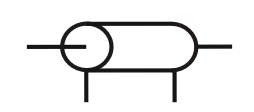
\includegraphics{translineSymbol}}

\device
\begin{alltt}
O<name> <A port (+) node> <A port (-) node>
+ <B port (+) node> <B port (-) node> [model name]
\end{alltt}

\model
\begin{alltt}
.MODEL <model name> LTRA R=<value> L=<value> C=<value>
+ G=<value> LEN=<value> [model parameters]
\end{alltt}

\examples
\begin{alltt}
Oline1 inp inn outp outn cable1
Oline2 inp inn outp outn cable1
\end{alltt}

\comments

The lossy transmission line, or LTRA, device is a two port (\texttt{A}
and \texttt{B}), bi-directional device. The \texttt{(+)} and \texttt{(-)} nodes
define the polarity of a positive voltage at a port.

\texttt{R}, \texttt{L}, \texttt{C}, and \texttt{G} are the resistance,
inductance, capacitance, and conductance of the transmission line per unit
length, respectively. \texttt{LEN} is the total length of the transmission
line. Supported configurations for the LTRA are \texttt{RLC}, \texttt{RC},
\texttt{LC} (lossless) and \texttt{RG}.

The lossy transmission line, or LTRA, device does not work with AC
analysis at this time.  LTRA models will need to be replaced with
lumped transmission line models (YTRANSLINE) when used in AC analysis.
The LTRA models do work correctly in harmonic balance simulation.
\end{Device}


%\paragraph{Device Parameters}
%% This table was generated by Xyce:
%   Xyce -doc O 1
%
\index{lossy transmission line!device instance parameters}
\begin{DeviceParamTableGenerated}{Lossy Transmission Line Device Instance Parameters}{O_1_Device_Instance_Params}
I1 & Initial current at end 1 & A & 0 \\ \hline
I2 & Initial current at end 2 & A & 0 \\ \hline
V1 & Initial voltage at end 1 & V & 0 \\ \hline
V2 & Initial voltage at end 2 & V & 0 \\ \hline
\end{DeviceParamTableGenerated}


\paragraph{Model Parameters}
% This table was generated by Xyce:
%   Xyce -doc O 1
%
\index{lossy transmission line!device model parameters}
\begin{DeviceParamTableGenerated}{Lossy Transmission Line Device Model Parameters}{O_1_Device_Model_Params}
ABS & Abs. rate of change of deriv. for bkpt & -- & 1 \\ \hline
C & Capacitance per unit length & F/m & 0 \\ \hline
COMPACTABS & special abstol for straight line checking & -- & 1e-12 \\ \hline
COMPACTREL & special reltol for straight line checking & -- & 0.001 \\ \hline
COMPLEXSTEPCONTROL & do complex time step control using local truncation error estimation & logical (T/F) & false \\ \hline
G & Conductance per unit length & $\mathsf{\Omega}^{-1}$ m$^{-1}$ & 0 \\ \hline
L & Inductance per unit length & Hm$^{-1}$ & 0 \\ \hline
LEN & length of line & m & 0 \\ \hline
LININTERP & use linear interpolation & logical (T/F) & false \\ \hline
MIXEDINTERP & use linear interpolation if quadratic results look unacceptable & logical (T/F) & false \\ \hline
NOSTEPLIMIT & don't limit timestep size based on the time constant of the line & logical (T/F) & false \\ \hline
QUADINTERP & use quadratic interpolation & logical (T/F) & true \\ \hline
R & Resistance per unit length & $\mathsf{\Omega}/$m & 0 \\ \hline
REL & Rel. rate of change of deriv. for bkpt & -- & 1 \\ \hline
STEPLIMIT & limit timestep size based on the time constant of the line & logical (T/F) & true \\ \hline
TRUNCDONTCUT & don't limit timestep to keep impulse response calculation errors low & logical (T/F) & false \\ \hline
TRUNCNR & use N-R iterations for step calculation in LTRAtrunc & logical (T/F) & false \\ \hline
\end{DeviceParamTableGenerated}


By default time step limiting is on in the LTRA. This means that
simulation step sizes will be reduced if required by the LTRA to
preserve accuracy. This can be disabled by setting
\texttt{NOSTEPLIMIT=1} and \texttt{TRUNCDONTCUT=1} on the
\texttt{.MODEL} line.

The option most worth experimenting with for increasing the speed of
simulation is \texttt{REL}. The default value of 1 is usually safe
from the point of view of accuracy but occasionally increases
computation time. A value greater than 2 eliminates all breakpoints
and may be worth trying depending on the nature of the rest of the
circuit, keeping in mind that it might not be safe from the viewpoint
of accuracy. Breakpoints may be entirely eliminated if the circuit
does not exhibit any sharp discontinuities. Values between 0 and 1 are
usually not required but may be used for setting many breakpoints.

\texttt{COMPACTREL} and \texttt{COMPACTABS} are tolerances that
control when the device should attempt to compact past history. This
can significantly speed up the simulation, and reduce memory usage,
but can negatively impact accuracy and in some cases may cause
problems with the nonlinear solver. In general this capability should
be used with linear type signals, such as square-wave-like
voltages. In order to activate this capability the general device
option \texttt{TRYTOCOMPACT=1} must be set, if it is not no history
compaction will be performed and the \texttt{COMPACT} options will be
ignored.

Example:

\texttt{.OPTIONS DEVICE TRYTOCOMPACT=1}

\paragraph{References}
See references \cite{Roychodhury:1994} and \cite{Spice3f5-user-guide} for more information
about the model.


%%
%% Voltage- or Current-controlled Switch Subsection
%%
\clearpage
\subsection{Voltage- or Current-controlled Switch}
\index{device!controlled switch} \index{controlled switch}
% Sandia National Laboratories is a multimission laboratory managed and
% operated by National Technology & Engineering Solutions of Sandia, LLC, a
% wholly owned subsidiary of Honeywell International Inc., for the U.S.
% Department of Energy’s National Nuclear Security Administration under
% contract DE-NA0003525.

% Copyright 2002-2019 National Technology & Engineering Solutions of Sandia,
% LLC (NTESS).


\begin{Device}

\device
\begin{alltt}
S<name> <(+) switch node> <(-) switch node>
+ <(+) control node> <(-) control node>
+ <model name> [ON] [OFF]

W<name> <(+) switch node> <(-) switch node>
+ <control node voltage source>
+ <model name> [ON] [OFF]
\end{alltt}

\model
\begin{alltt}
.MODEL <model name> VSWITCH [model parameters]
.MODEL <model name> ISWITCH [model parameters]
\end{alltt}

\examples
\begin{alltt}
S1 21 23 12 10 SMOD1
SSET 15 10 1 13 SRELAY
W1 1 2 VCLOCK SWITCHMOD1
W2 3 0 VRAMP SM1 ON
\end{alltt}

\comments

The voltage- or current-controlled switch is a particular type of
controlled resistor. This model is designed to help reduce numerical
issues. See Special Considerations below.

The resistance between the \texttt{<(+) switch node>} and the
\texttt{<(-) switch node>} is dependent on either the voltage between
the \texttt{<(+) control node>} and the \texttt{<(-) control node>} or
the current through the control node voltage source. The resistance
changes in a continuous manner between the \texttt{RON} and
\texttt{ROFF} model parameters.

No resistance is inserted between the control nodes.  It is up to the
user to make sure that these nodes are not floating.

Even though evaluating the switch model is computationally
inexpensive, for transient analysis \Xyce{} steps through the
transition section using small time-steps in order to calculate the
waveform accurately. Thus, a circuit with many switch transitions can
result in lengthy run times.

The ON and OFF parameters are used to specify the initial state of the
switch at the first step of the operating point calculation; this does
not force the switch to be in that state, it only gives the operating
point solver an initial state to work with.  If it is known that the
switch should be in a particular state in the operating point it could
help convergence to specify one of these keywords.

The power dissipated in the switch is calculated with $I \cdot \Delta V$ 
where the voltage drop is calculated as $(V_+ - V_-)$ and positive current 
flows from $V_+$ to $V_-$.  This will essentially be the power dissipated
in either \texttt{RON} or \texttt{ROFF}, since the switch is a particular 
type of controlled resistor.

\end{Device}

\pagebreak

\paragraph{Model Parameters}
% This table was generated by Xyce:
%   Xyce -doc S 1
%
\index{controlled switch!device model parameters}
\begin{DeviceParamTableGenerated}{Controlled Switch Device Model Parameters}{S_1_Device_Model_Params}
IOFF & Off current & A & 0 \\ \hline
ION & On current & A & 0.001 \\ \hline
OFF & Off control value & -- & 0 \\ \hline
ON & On control value & -- & 1 \\ \hline
ROFF & Off resistance & $\mathsf{\Omega}$ & 1e+06 \\ \hline
RON & On resistance & $\mathsf{\Omega}$ & 1 \\ \hline
VOFF & Off voltage & V & 0 \\ \hline
VON & On voltage & V & 1 \\ \hline
\end{DeviceParamTableGenerated}


\paragraph{Special Considerations}

\begin{XyceItemize}
\item Due to numerical limitations, \Xyce{} can only manage a dynamic range of
  approximately 12 decades.  Thus, it is recommended the user limit the ratio
  \textrmb{ROFF}/\textrmb{RON} to less than $10^{12}$.  This soft limitation is not enforced by the code, and larger ratios might converge for some problems.
\item Do not set \textrmb{RON} to 0.0, as the code computes the ``on'' conductance as the inverse of \textrmb{RON}.  Using 0.0 will cause the simulation to fail when this invalid division results in an infinite conductance.  Use a very small, but non-zero, on resistance instead.
\item Furthermore, it is a good idea to limit the narrowness of the transition
  region. This is because in the transition region, the switch has gain and the
  narrower the region, the higher the gain and the more potential for numerical
  problems.  The smallest value recommended for $\|\mathbf{VON - VOFF}\|$ or
  $\|\mathbf{ION - IOFF}\|$ is $1\times10^{-12}$.  This recommendation is not a restriction, and you might find for some problems that narrower transition regions might work well.
\end{XyceItemize}

\paragraph{Controlled switch equations}
The equations in this section use the following variables:
\[
\begin{array}{rllll}
R_s & = & \mbox{switch resistance} \\
V_c & = & \mbox{voltage across control nodes} \\
I_c & = & \mbox{current through control node voltage source} \\
L_m & = & \mbox{log-mean of resistor values} & = &
\ln \left(\sqrt{\mathbf{RON \cdot ROFF}} \right) \\
L_r & = & \mbox{log - ratio of resistor values} & = &
\ln \left(\mathbf{RON / ROFF} \right) \\
V_d & = & \mbox{difference of control voltages} & = & \mathbf{VON - VOFF} \\
I_d & = & \mbox{difference of control currents} & = & \mathbf{ION - IOFF} \\
\end{array}
\]

\subparagraph{Switch Resistance}

To compute the switch resistance, \Xyce{} first calculates the
``switch state'' $S$ as $S=(V_c-\mathbf{VOFF})/V_d$ or
$S=(I_c-\mathbf{IOFF})/I_d$.  The switch resistance is then:
\[ R_s = \left\{ \begin{array}{ll}
\mathbf{RON}, & S \geq 1.0 \\
\mathbf{ROFF}, & S \leq 0.0 \\
\exp \left(L_m + 0.75L_r(2S-1) - 0.25L_r(2S-1)^3 \right),
& 0< S < 1
\end{array}
\right.
\]

%\subparagraph{Noise}
%Noise is computed using a 1.0 Hz bandwidth.  The voltage-controlled switch
%produces thermal noise as though it were a resistor with the resistance a
%switch has at its bias point.  It uses a spectral power density (per unit
%bandwidth):
%\[
%i^2 = 4kT/R_s
%\]


%%
%% Generic Switch Subsection
%%
\clearpage
\subsection{Generic Switch}
\index{device!generic switch} \index{generic switch}
% Sandia National Laboratories is a multimission laboratory managed and
% operated by National Technology & Engineering Solutions of Sandia, LLC, a
% wholly owned subsidiary of Honeywell International Inc., for the U.S.
% Department of Energy’s National Nuclear Security Administration under
% contract DE-NA0003525.

% Copyright 2002-2020 National Technology & Engineering Solutions of Sandia,
% LLC (NTESS).


\begin{Device}

\device
SW<name> <(+) switch node> <(-) switch node> <model name> [ON] [OFF] <control = { expression }>

\model
\begin{alltt}
.MODEL <model name> VSWITCH [model parameters]
.MODEL <model name> ISWITCH [model parameters]
.MODEL <model name> SWITCH [model parameters]
\end{alltt}

\examples
\begin{alltt}
SW 1 2 SWI OFF CONTROL=\{I(VMON)\}
SW 1 2 SWV OFF CONTROL=\{V(3)-V(4)\}
SW 1 2 SW OFF CONTROL=\{if(time>0.001,1,0)\}
\end{alltt}

\comments

The generic switch is similar to the voltage- or current-controlled
switch except that the control variable is anything that can be writen
as an expression.  The examples show how a voltage- or
current-controlled switch can be implemented with the generic switch.
Also shown is a relay that turns on when a certain time is reached.
Model parameters are given in Table ~\ref{S_1_Device_Model_Params}.

The power dissipated in the generic switch is calculated with $I \cdot \Delta V$ 
where the voltage drop is calculated as $(V_+ - V_-)$ and positive current 
flows from $V_+$ to $V_-$.  This will essentially be the power dissipated
in either \texttt{RON} or \texttt{ROFF}, since the generic switch is a particular 
type of controlled resistor.

\end{Device}


%%
%% YLIN device Subsection
%%
\clearpage
\subsection{Linear device}
\index{linear device}
% Sandia National Laboratories is a multimission laboratory managed and
% operated by National Technology & Engineering Solutions of Sandia, LLC, a
% wholly owned subsidiary of Honeywell International Inc., for the U.S.
% Department of Energy’s National Nuclear Security Administration under
% contract DE-NA0003525.

% Copyright 2002-2022 National Technology & Engineering Solutions of Sandia,
% LLC (NTESS).

The linear (YLIN) device allows an S-, Y-, or Z-parameter model to
be used to define an N-port device.  It is mostly commonly used
as part of a Harmonic Balance (HB) analysis.

\begin{Device}\label{YLIN_DEVICE}

\device
\begin{alltt}
YLIN <name>  <(+) node> <(-) node> [model name]
\end{alltt}

\model
.MODEL <model name> LIN [model parameters]

\examples
\begin{alltt}
YLIN YLIN1 1 0 2 0 YLIN_MOD1
.MODEL YLIN_MOD1 LIN TSTONEFILE=yparams.y2p
\end{alltt}

\parameters
\begin{Parameters}

\param{model name}
  Name of the model defined in a .MODEL line.

\end{Parameters}

\comments
At present, the YLIN device is only supported in the frequency domain for HB analyses.

\end{Device}


\paragraph{Model Parameters}
% This table was generated by Xyce:
%   Xyce -doc Lin 1
%
\index{lin!device model parameters}
\begin{DeviceParamTableGenerated}{LIN Device Model Parameters}{Lin_1_Device_Model_Params}
ISC\_FD & Touchstone file contains frequency-domain short-circuit current data & logical (T/F) & false \\ \hline
%ISC\_TD\_FILE & ISC Time Domain File Name & -- & '' \\ \hline
%ISC\_TD\_FILE\_FORMAT & Format of ISC Time Domain File & -- & 'STD' \\ \hline
TSTONEFILE & Touchstone File Name & -- & '' \\ \hline
\end{DeviceParamTableGenerated}


The Touchstone file name must be specified.  The YLIN device accepts both
Touchstone 1 and Touchstone 2 formatted input files \cite{touchstone2_std_2009}.

For coupling with EM codes, such as EIGER, the YLIN device also accepts
a non-standard version of the Touchstone input files.  If the \texttt{ISC\_FD}
model parameter is set to true then each row of ``network data'' in the input
file also contains additional columns with the ``per-port frequency-domain
short-circuit currents''.   There are then two such additional columns for each
port.  The format (\texttt{RI}, \texttt{MA} or \texttt{DB}) of those additional
columns will be as specified by the Option line in the Touchstone file.  In this
non-standard case, only the ``Full'' matrix format is supported for
Touchstone 2 input files.






%%
%% Lossless, Ideal Transmission Line Subsection
%%
\clearpage
\subsection{Lossless (Ideal) Transmission Line}
\index{device!lossless transmission line} \index{lossless transmission line}
\index{device!transmission line!lossless}
% Sandia National Laboratories is a multimission laboratory managed and
% operated by National Technology & Engineering Solutions of Sandia, LLC, a
% wholly owned subsidiary of Honeywell International Inc., for the U.S.
% Department of Energy’s National Nuclear Security Administration under
% contract DE-NA0003525.

% Copyright 2002-2020 National Technology & Engineering Solutions of Sandia,
% LLC (NTESS).


\begin{Device}\label{T_DEVICE}

\symbol
{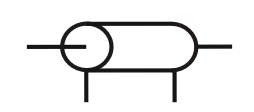
\includegraphics{translineSymbol}}

\device
\begin{alltt}
T<name> <port 1 (+) node> <port 1 (-) node>
+ <port 2 (+) node> <port 2 (-) node>
+ Z0=<value> [TD=<value>] [F=<value> [NL=<value>]]
\end{alltt}

\examples
\begin{alltt}
Tline inp inn outp outn Z0=50 TD=1us
Tline2 inp inn outp outn Z0=50 F=1meg NL=1.0
\end{alltt}

\comments

The lossless transmission line device is a two port (\texttt{A} and
\texttt{B}), bi-directional delay line. The \texttt{(+)} and
\texttt{(-)} nodes define the polarity of a positive voltage at a port.

\texttt{Z0} is the characteristic impedance. For user convenience, 
\texttt{ZO} (``Zee Oh'') is an allowed synonym for \texttt{Z0} (``Zee Zero'').

The transmission line's length is specified by either \texttt{TD} (a delay in
seconds) or by the combination of \texttt{F} and \texttt{NL} (a frequency in Hz and 
the relative wavelength at \texttt{F}). \texttt{NL} defaults to 0.25 (\texttt{F} is 
the quarter-wave frequency).  If \texttt{F} is given, the time delay is 
computed as $\frac{NL}{F}$.  

While both \texttt{TD} and \texttt{F} are optional, at least one of them must be given.
It is an instance line error if both are given.

Lead currents for the two terminals (1 and 2) of the lossless transmission device 
(e.g.,for the T device \texttt{line2}) are accessed via \texttt{I1(Tline2)} and 
\texttt{I2(Tline2)}.  The polarity conventions are that positive current flows into
the positive node of the specified terminal, and negative current flows out of the
positive node of the specified terminal.

Power for the lossless transmission line is calculated as $I_1 \cdot \Delta V_1 + 
I_2 \cdot \Delta V_2$, where the voltage drops ($\Delta V_1$ and $\Delta V_2$) are the 
voltage drops between the positive and negative terminals of each port (e.g., 
$\Delta V = (V_+ - V_-)$).  The sign conventions for the lead currents $I_1$ and $I_2$ 
were given in the previous paragraph.  This definition can be viewed as the instantaneous
sum of the power flowing into terminal 1 and the power flowing into terminal 2.
This definition for power for the lossless transmission line may differ from 
commercial simulators, such as HSPICE.  

The lossless transmission line device does not work with AC analysis
at this time.  Lossless transmission line models will need to be
replaced with lumped transmission line models (YTRANSLINE) when used
in AC analysis.  The lossless transmission line does work correctly in
harmonic balance simulation.

\end{Device}

\paragraph{Instance Parameters}
% This table was generated by Xyce:
%   Xyce -doc T 1
%
\index{ideal transmission line!device instance parameters}
\begin{DeviceParamTableGenerated}{Ideal Transmission Line Device Instance Parameters}{T_1_Device_Instance_Params}
F & Frequency & Hz & 0 \\ \hline
NL & Length in wavelengths & -- & 0.25 \\ \hline
TD & Time delay & s & 0 \\ \hline
Z0 & Characteristic Impedance & $\mathsf{\Omega}$ & 0 \\ \hline
ZO & Characteristic Impedance & $\mathsf{\Omega}$ & 0 \\ \hline
\end{DeviceParamTableGenerated}



%%
%% Lumped Transmission Line Subsection
%%
\clearpage
\subsection{Lumped Transmission Line}
\index{device!lumped transmission line} \index{lumped transmission line}
\index{device!transmission line!lumped}
% Sandia National Laboratories is a multimission laboratory managed and
% operated by National Technology & Engineering Solutions of Sandia, LLC, a
% wholly owned subsidiary of Honeywell International Inc., for the U.S.
% Department of Energy’s National Nuclear Security Administration under
% contract DE-NA0003525.

% Copyright 2002-2019 National Technology & Engineering Solutions of Sandia,
% LLC (NTESS).


\begin{Device}

\symbol
{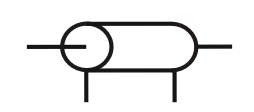
\includegraphics{translineSymbol}}

\device
\begin{alltt}
ytransline <name> <Input port> <Output port> testLine 
+ len=<value> lumps=<value>
\end{alltt}

\model
\begin{alltt}
.model testLine transline r=<value> l=<value> 
+ c=<value> [model parameters]
\end{alltt}

\examples
\begin{alltt}
ytransline line1 inn out  testLine len=12.0 lumps=1440
\end{alltt}

\comments
The lumped transmission line, device is a two port bi-directional device.   The specification
is patterned, loosely, from the netlist specification for the LTRA device.

\texttt{R}, \texttt{L}, and \texttt{C}  are the resistance,
inductance, and capacitance of the transmission line per unit
length, respectively. \texttt{LEN} is the total length of the transmission
line, and \texttt{LUMPS} is the number of lumped elements used to discretize the line. 
Supported configurations for this device are \texttt{RLC} and \texttt{LC}.

Unlike the LTRA device, which is based on an analytic solution, this device is 
based on assembling chains of linear R,L and C devices to approximate the 
solution to the Telegraph equations.  It is the functional equivalent of building a
transmission line in the netlist using subcircuits of linear elements.  The advantage
of using this approach is that it automates the mechanics of this process, and
thus is less prone to error.  It can be used with all analysis types, including
harmonic balance (HB).

The model is based on the assumption that the segments of the line are evenly spaced.
The number of segments is specified by the parameter \texttt{LUMPS} and the larger 
this number, the more accurate the calculation.
\end{Device}

\paragraph{Device Parameters}
% This table was generated by Xyce:
%   Xyce -doc Transline 1
%
\index{lumped transmission line!device instance parameters}
\begin{DeviceParamTableGenerated}{Lumped Transmission Line Device Instance Parameters}{Transline_1_Device_Instance_Params}
LEN & length of line & m & 0 \\ \hline
LUMPS &  & -- & 1 \\ \hline
\end{DeviceParamTableGenerated}


\paragraph{Model Parameters}
% This table was generated by Xyce:
%   Xyce -doc Transline 1
%
\index{lumped transmission line!device model parameters}
\begin{DeviceParamTableGenerated}{Lumped Transmission Line Device Model Parameters}{Transline_1_Device_Model_Params}
C & Capacitance per unit length & F/m & 0 \\ \hline
ELEV &  & -- & 2 \\ \hline
G & Conductance per unit length & $\mathsf{\Omega}^{-1}$ m$^{-1}$ & 0 \\ \hline
L & Inductance per unit length & Hm$^{-1}$ & 0 \\ \hline
R & Resistance per unit length & $\mathsf{\Omega}/$m & 0 \\ \hline
\end{DeviceParamTableGenerated}



%\paragraph{References}
%%See references \cite{Roychodhury:1994} and \cite{Spice3f5-user-guide} for more information
%about the model.


%%
%% Delay device Subsection
%%
\clearpage
\subsection{Ideal Delay}
\index{device!delay device}
\index{device!ideal delay device}
% Sandia National Laboratories is a multimission laboratory managed and
% operated by National Technology & Engineering Solutions of Sandia, LLC, a
% wholly owned subsidiary of Honeywell International Inc., for the U.S.
% Department of Energy’s National Nuclear Security Administration under
% contract DE-NA0003525.

% Copyright 2002-2022 National Technology & Engineering Solutions of Sandia,
% LLC (NTESS).


An ideal delay device, operating in a manner similar to a
voltage-controlled voltage source, is provided by the YDELAY device.

\begin{Device}

\device
\begin{alltt}
YDELAY <name> <positive node> <negative node>
+ <positive control node> <negative control node>
+ TD=<time delay>
+ [EXTRAPOLATION=<true|false>] [BPENABLED=<true|false>]
+ [LINEARINTERP=<true|false>] 
\end{alltt}

\examples
\begin{alltt}
YDELAY delay1 2 0 1 0 TD=10N
R1 2 0 1
YDELAY delay1 3 0 2 0 TD=10N LINEARINTERP=true
R2 3 0 1
YDELAY delay1 4 0 3 0 TD=10N BPENABLED=FALSE
R4 4 0 1
YDELAY delay1 5 0 4 0 TD=10N EXTRAPOLATION=false
R5 5 0 1
\end{alltt}

\comments

The voltage between the positive and negative control nodes is
reproduced at the positive and negative output nodes delayed by a time
equal to the specified TD parameter.

The device is equivalent in connectivity to a voltage-controlled
voltage source --- the device puts no load on the control nodes, and
its output must be connected to a valid circuit.

Unlike the transmission line, no impedance matching is required, and
reflections due to impedance mismatch do not occur.

These devices may be chained to create outputs at different delays,
but each instance must have its output connected to a valid closed
circuit.  The examples above are chained correctly so that each of the
output nodes is delayed by 10 nanoseconds from the previous stage.

The device functions by storing a history of its input at each
accepted time point.  At each new time step, interpolation is
performed on this history to determine what the signal would have been
at a time TD in the past.  At each step, the device checks its history
to determine if the previous three saved steps include a discontinuity
in the input.  If so, the device assures that \Xyce{} will correctly
resolve the same discontinuity when it appears on the output.

With no special options specified, three-point quadratic interpolation
is used except after a discontinuity, when linear interpolation is
performed.  If \Xyce{} has advanced the time by more than TD and no
discontinuity has occured, then this interpolation is actually
extrapolation.

When \texttt{LINEARINTERP=true} is specified, the history
interpolation used is always linear interpolation.

When \texttt{EXTRAPOLATION=false}, \Xyce{} will never attempt
extrapolation when it has taken a time step larger than TD.  In this
case, the current, unconverged value of the solution is used as the
third interpolation point and the interpolation is recomputed at every
step of the nonlinear solve.

When \texttt{BPENABLED=false}, the device will not set a simulation
breakpoint to force the time integrator to stop exactly TD seconds
after a detected discontinuity on the input.  It will still force a
maximum time step on the time integrator after such a discontinuity,
and other techniques will be applied to assure the discontinuity is
resolved.  This option may result in \Xyce{} rejecting a lot more time
steps and slower simulation than when it is left at its default.

\end{Device}

\subsubsection{Delay device instance parameters}

The instance parameters for the delay device are shown in
Table~\ref{Delay_1_Device_Instance_Params}.

% This table was generated by Xyce:
%   Xyce -doc Delay 1
%
\index{delay element!device instance parameters}
\begin{DeviceParamTableGenerated}{Delay element Device Instance Parameters}{Delay_1_Device_Instance_Params}
BPENABLED & Can this device set discontinuity breakpoints? & -- & true \\ \hline
EXTRAPOLATION & Can this device use extrapolation on history? & -- & true \\ \hline
LINEARINTERP & Should this device use only linear interpolation on history? & -- & false \\ \hline
TD & Time delay & s & 0 \\ \hline
\end{DeviceParamTableGenerated}


%%
%% U Type Digital Device
%%
\clearpage
\subsection{Behavioral Digital Devices}
\index{device!digital devices} \index{digital devices}
% Sandia National Laboratories is a multimission laboratory managed and
% operated by National Technology & Engineering Solutions of Sandia, LLC, a
% wholly owned subsidiary of Honeywell International Inc., for the U.S.
% Department of Energy’s National Nuclear Security Administration under
% contract DE-NA0003525.

% Copyright 2002-2019 National Technology & Engineering Solutions of Sandia,
% LLC (NTESS).

 
%%
%% Behavioral Digital Description Table
%%
\begin{Device}\label{U_DEVICE}

 
\device
\begin{alltt}
U<name> <type>(<num inputs>) [digital power node] 
+ [digital ground node] <input node>* <output node>* 
+ <model name> [device parameters]
\end{alltt}
 
\model
.MODEL <model name> DIG [model parameters]
 
\examples
\begin{alltt}
UMYAND AND(2) DPWR DGND in1 in2 out DMOD IC=TRUE
UTHEINV INV DPWR DGND in out DMOD
.model DMOD DIG (
+ CLO=1e-12  CHI=1e-12
+ S0RLO=5  S0RHI=5  S0TSW=5e-9
+ S0VLO=-1  S0VHI=1.8
+ S1RLO=200  S1RHI=5  S1TSW=5e-9
+ S1VLO=1  S1VHI=3
+ RLOAD=1000
+ CLOAD=1e-12
+ DELAY=20ns )
\end{alltt}

\parameters 
\begin{Parameters}

\param{type} 

Type of digital device.  Supported devices are: INV, BUF, AND, NAND, OR, NOR, XOR,
NXOR, DFF, JKFF, TFF, DLTCH and ADD.  (Note: NOT is an allowed synonym for INV, but will be
deprecated in future \Xyce{} releases.)

The following gates have a fixed number of inputs.  INV and BUF have only one
input and one output node.  XOR and NXOR have two inputs and one output.
ADD has three inputs (in1, in2, carryIn) and two outputs (sumOut
and carryOut).  DFF has four inputs (PREB, CLRB, Clock and Data) and
two outputs ($Q$ and $\bar{Q}$).  TFF has two inputs (T and CLK) and two
outputs ($Q$ and $\bar{Q}$).  The TFF uses ``positive'' (``rising'') edge clocking.
The JKFF has five inputs (PREB, CLRB, Clock, J and K) and two outputs ($Q$ and $\bar{Q}$).
The JKFF uses ``negative'' (``falling'') edge clocking.
DLTCH has four inputs (PREB, CLRB, Enable and Data) and two outputs ($Q$ and $\bar{Q}$).  

The AND, NAND, OR and NOR gates have one output but a variable number of inputs.  
There is no limit on the number of inputs for AND, NAND, OR and NOR gates, but
there must be at least two inputs.

\param{num inputs}

For AND, NAND, OR and NOR gates, with N inputs, the syntax is (N), as shown for the
MYAND example given above, where AND(2) is specified.  The inclusion of (N) is mandatory
for gates with a variable number of inputs, and both the left and right parentheses must
be used to enclose N.  

This parameter is optional, and typically omitted, for gates with a fixed number of
inputs, such as INV, BUF, XOR, NXOR, DFF, JKFF, TFF, DLTCH and ADD.  This is illustrated by the THEINV
example given above, where the device type is INV rather than INV(1).

\param{digital power node}

Dominant node to be connected to the output node(s) to establish high
output state.  This node is connected to the output by a resistor and
capacitor in parallel, whose values are set by the model.  This node must
be specified on the instance line.

\param{digital ground node}

This node serves two purposes, and must be specified on the instance line.
It is the dominant node to be connected to the output node(s) to establish
low output state.  This node is connected to the output by a resistor and 
capacitor in parallel, whose values are set by the model.  This node is also
connected to the input node by a resistor and capacitor in parallel, whose
values are set by the model.  Determination of the input state is based on the
voltage drop between the input node and this node.

\param{input nodes, output nodes}

Input and output nodes that connect to the circuit.

\param{model name}

 Name of the model defined in a .MODEL line.

\param{device parameters}

Parameter listed in Table~\ref{Digital_1_Device_Instance_Params_Udevice} may be
provided as \texttt{<parameter>=<value>} specifications as needed.  For
devices with more than one output, multiple output initial states may be
provided as Boolean values in either a comma separated list (e.g.
IC=TRUE,FALSE for a device with two outputs) or individually 
(e.g. IC1=TRUE IC2=FALSE or IC2=FALSE).  Finally, the IC specification
must use TRUE and FALSE rather than T and F.

\end{Parameters}
\end{Device}

\paragraph{Device Parameters}

%%
%% Digital Device Param Table
%%
% Sandia National Laboratories is a multimission laboratory managed and
% operated by National Technology & Engineering Solutions of Sandia, LLC, a
% wholly owned subsidiary of Honeywell International Inc., for the U.S.
% Department of Energy’s National Nuclear Security Administration under
% contract DE-NA0003525.

% Copyright 2002-2022 National Technology & Engineering Solutions of Sandia,
% LLC (NTESS).

% This table was generated by Xyce:
%   Xyce -doc Digital 1
%
\index{behavioral digital!device instance parameters}
\begin{DeviceParamTableGenerated}{Behavioral Digital Device Instance Parameters}{Digital_1_Device_Instance_Params_Udevice}
IC1 & Vector of initial values for output(s) & logical (T/F) & false \\ \hline
IC2 &  & -- & false \\ \hline
\end{DeviceParamTableGenerated}


\paragraph{Model Parameters}

%%
%% Digital Model Param Table
%%
% Sandia National Laboratories is a multimission laboratory managed and
% operated by National Technology & Engineering Solutions of Sandia, LLC, a
% wholly owned subsidiary of Honeywell International Inc., for the U.S.
% Department of Energy’s National Nuclear Security Administration under
% contract DE-NA0003525.

% Copyright 2002-2019 National Technology & Engineering Solutions of Sandia,
% LLC (NTESS).

% This table was generated by Xyce:
%   Xyce -doc Digital 1
%
\index{behavioral digital!device model parameters}
\begin{DeviceParamTableGenerated}{Behavioral Digital Device Model Parameters}{Digital_1_Device_Model_Params_Udevice}
CHI & Capacitance between output node and high reference & F & 1e-06 \\ \hline
CLO & Capacitance between output node and low reference & F & 1e-06 \\ \hline
CLOAD & Capacitance between input node and input reference & F & 1e-06 \\ \hline
DELAY & Delay time of device & s & 1e-08 \\ \hline
RLOAD & Resistance between input node and input reference & $\mathsf{\Omega}$ & 1000 \\ \hline
S0RHI & Low state resitance between output node and high reference & $\mathsf{\Omega}$ & 100 \\ \hline
S0RLO & Low state resistance between output node and low reference & $\mathsf{\Omega}$ & 100 \\ \hline
S0TSW & Switching time transition to low state & s & 1e-08 \\ \hline
S0VHI & Maximum voltage to switch to low state & V & 1.7 \\ \hline
S0VLO & Minimum voltage to switch to low state & V & -1.5 \\ \hline
S1RHI & High state resistance between output node and high reference & $\mathsf{\Omega}$ & 100 \\ \hline
S1RLO & High state resistance between output node and low reference & $\mathsf{\Omega}$ & 100 \\ \hline
S1TSW & Switching time transition to high state & s & 1e-08 \\ \hline
S1VHI & Maximum voltage to switch to high state & V & 7 \\ \hline
S1VLO & Minimum voltage to switch to high state & V & 0.9 \\ \hline
\end{DeviceParamTableGenerated}


\paragraph{Model Description}

The input interface model consists of the input node connected with a resistor and
capacitor in parallel to the digital ground node.  The values of these are: \textrmb{RLOAD}
and \textrmb{CLOAD}.  

The logical state of any input node is determined by comparing the voltage relative
to the reference to the range for the low and high state.  The range for the low
state is \textrmb{S0VLO} to \textrmb{S0VHI}.  Similarly, the range for the high state
is \textrmb{S1VLO} to \textrmb{S1VHI}.  The state of an input node will remain fixed as
long as its voltage stays within the range for its current state.  That input node will
transition to the other state only when its state goes outside the voltage range of
its current state.

The output interface model is more complex than the input model, but shares the same
basic configuration of a resistor and capacitor in parallel to simulate loading.  For
the output case, there are such parallel RC connections to two nodes, the digital
ground node and the digital power node.  Both of these nodes must be specified on
the instance line.

The capacitance to the high node is specified by \textrmb{CHI}, and the capacitance to the low
node is \textrmb{CLO}.  The resistors in parallel with these capacitors are variable, and have
values that depend on the state.  In the low state (S0), the resistance values are:
\textrmb{S0RLO} and \textrmb{S0RHI}.  In the high state (S1) ,the resistance values are: 
\textrmb{S1RLO} and \textrmb{S1RHI}.  Transition to the high state occurs exponentially over
a time of \textrmb{S1TSW}, and to the low state \textrmb{S0TSW}.

The device's delay is given by the model parameter \textrmb{DELAY}.  Any input changes
that affect the device's outputs are propagated after this delay.

As a note, the model parameters \textrmb{VREF}, \textrmb{VLO} and \textrmb{VHI} are used
by the now deprecated Y-type digital device, but are
ignored by the U device.  A warning message is emitted if any of these three parameters
are used in the model card for a U device.

Another caveat is that closely spaced input transitions to the \Xyce{} digital behavioral
models may not be accurately reflected in the output states.  In particular, input-state
changes spaced by more than \texttt{DELAY} seconds have independent effects on the output
states. However, two input-state changes (S1 and S2) that occur within \texttt{DELAY} seconds
(e.g., at time=t1 and time=t1+0.5*\texttt{DELAY}) have the effect of masking the effects
of S1 on the device's output states, and only the effects of S2 are propagated to the
device's output states.

\paragraph{DCOP Calculations for Flip-Flops and Latches}
The behavior of the digital devices during the DC Operating Point (DCOP) calculations
can be controlled via the \texttt{IC1} and \texttt{IC2} instance parameters and the
\texttt{DIGINITSTATE} device option.  See ~\ref{Options_Reference} for more details on the
syntax for device options.  Also, this section applies to the Y-Type Behavioral Digital Devices
discussed in ~\ref{YTypeDigitalDevice}.

The \texttt{IC1} instance parameter is supported for all gate types.  The \texttt{IC2}
instance parameter is supported for all gate types that have two outputs.  These instance
parameters allow the outputs of individual gates to be set to known states (either
\texttt{TRUE (1)} or \texttt{FALSE (0)}) during the DCOP calculation, irregardless of their 
input state(s).  There are two caveats.  First, the \texttt{IC1} and \texttt{IC2} settings 
at a given gate will override the global effects of the \texttt{DIGINITSTATE} option, 
discussed below, at that gate.  Second, \texttt{IC1} and \texttt{IC2} do not support the
\texttt{X}, or ``undetermined'', state discussed below.

The \texttt{DIGINITSTATE} option only applies to the DLTCH, DFF, JKFF and TFF devices.  It was added
for improved compatibility with PSpice.  It sets the initial state of all flip-flops and 
latches in the circuit: 0=clear, 1=set, 2=\texttt{X}.  At present, the use of the
\texttt{DIGINITSTATE} option during the DCOP is the only place that \Xyce{} supports the
\texttt{X}, or ``undetermined'', state.  The \texttt{X} state is modeled in \Xyce{} by having the
DLTCH, DFF, JKFF and TFF outputs simultaneously ``pulled-up'' and ``pulled-down''.  That approach typically 
produces an output level, for the \texttt{X} state, that is approximately halfway between the 
voltage levels for \texttt{TRUE} and \texttt{FALSE} (e.g., halfway between \texttt{V\_HI} and 
\texttt{V\_LO}). As mentioned above, the \texttt{IC1} and
\texttt{IC2} instance parameters take precedence at a given gate.

\Xyce{} also supports a default \texttt{DIGINITSTATE}, whose value is 3.  For this default value,
for the DFF, JKFF, TFF and DLTCH devices, \Xyce{} enforces $Q$ and $\bar{Q}$ being different at DCOP, if 
both \texttt{PREB} and \texttt{CLRB} are \texttt{TRUE} . The behavior of the DFF, JKFF and DLTCH 
devices at the DCOP for \texttt{DIGINITSTATE=3} is shown in Tables ~\ref{dffTruthTable},  ~\ref{jkffTruthTable}
and ~\ref{dltchTruthTable}.  In these three tables, the $X$ state denotes the ``Don't Care'' 
condition, where the input state can be 0, 1 or the ``undetermined'' state.
The first row in each truth-table (annotated with $*$) is ``unstable'', and will change to 
a state with $Q$ and $\bar{Q}$ being different once both \texttt{PREB} and \texttt{CLRB} are not 
both in the \texttt{FALSE} state.

The behavior of the TFF device at the DCOP, for the default \texttt{DIGINITSTATE} of 3, is
simpler, and is not shown as a table.  The design decision was to have $Q$ and $\bar{Q}$ be
different, with the $Q$ value equal to the state of the $T$ input.

%%
%% DFF Truth Table for DIGINITSTATE=3
%%
\LTXtable{\textwidth}{dffTruthTableTbl}

%%
%% DLTCH Truth Table for DIGINITSTATE=3
%%
\LTXtable{\textwidth}{dltchTruthTableTbl}

%%
%% JKFF Truth Table for DIGINITSTATE=3
%%
\LTXtable{\textwidth}{jkffTruthTableTbl}


%%
%% Behavioral Digital Devices - Y Type now deprecated
%%
\clearpage
\subsection{Y-Type Behavioral Digital Devices (Deprecated)}
\index{device!digital devices, Y type} \index{Y type digital devices}
% Sandia National Laboratories is a multimission laboratory managed and
% operated by National Technology & Engineering Solutions of Sandia, LLC, a
% wholly owned subsidiary of Honeywell International Inc., for the U.S.
% Department of Energy’s National Nuclear Security Administration under
% contract DE-NA0003525.

% Copyright 2002-2022 National Technology & Engineering Solutions of Sandia,
% LLC (NTESS).

 
%%
%% Behavioral Digital Description Table
%%
\begin{Device}\label{YTypeDigitalDevice}

\device
\begin{alltt}
Y<type> <name> [low output node] [high output node]
+ [input reference node] <input node>* <output node>*
+  <model name> [device parameters]
\end{alltt}

\model
.MODEL <model name> DIG [model parameters]

\examples
\begin{alltt}
YAND MYAND in1 in2 out DMOD IC=TRUE
YNOT THENOT in out DMOD
YNOR ANOR2 vlo vhi vref in1 in2 out DDEF
.model DMOD DIG (
+ CLO=1e-12  CHI=1e-12
+ S0RLO=5  S0RHI=5  S0TSW=5e-9
+ S0VLO=-1  S0VHI=1.8
+ S1RLO=200  S1RHI=5  S1TSW=5e-9
+ S1VLO=1  S1VHI=3
+ RLOAD=1000
+ CLOAD=1e-12
+ VREF=0 VLO=0 VHI=3
+ DELAY=20ns )
.MODEL DDEF DIG
\end{alltt}

\parameters
\begin{Parameters}

\param{type}
Type of digital device.  Supported devices are: NOT, BUF, AND, NAND, OR, NOR, XOR,
NXOR, DFF, JKFF, TFF, DLTCH and ADD.  (Note: INV is now the preferred synonym for NOT.  
The NOT device type will be deprecated in future \Xyce{} releases.)  For Y-type digital
devices, all devices have two input nodes and one output node, except for NOT, DFF and
ADD.  NOT has one input and one output.  ADD has three inputs (in1, in2, carryIn) and 
two outputs (sumOut and carryOut).  DFF has four inputs (PREB, CLRB, Clock and
Data) and two outputs ($Q$ and $\bar{Q}$). TFF has two inputs (T and Clock) and two
outputs ($Q$ and $\bar{Q}$).  The TFF uses ``positive'' (``rising'') edge clocking.
The JKFF has five inputs (PREB, CLRB, Clock, J and K) and two outputs ($Q$ and $\bar{Q}$).
The JKFF uses ``negative'' (``falling'') edge clocking.
DLTCH has four inputs (PREB, CLRB, Enable and Data) and two outputs ($Q$ and $\bar{Q}$). 

\param{name} 
Name of the device instance.  This must be present, and when combined
with the \texttt{Y<type>}, must be unique in the netlist.  In the
examples, MYAND, THENOT and ANOR2 have been used as names for the three
devices.

\param{low output node}

Dominant node to be connected to the output node(s) to establish low
output state.  This node is connected to the output by a resistor and
capacitor in parallel, whose values are set by the model.  If specified
by the model, this node must be omitted from the instance line and a
fixed voltage \textrmb{VLO} is used instead.

\param{high output node}

Dominant node to be connected to the output node(s) to establish high
output state.  This node is connected to the output by a resistor and
capacitor in parallel, whose values are set by the model.  If specified
by the model, this node must be omitted from the instance line and a fixed
voltage \textrmb{VHI} is used instead.

\param{input reference node}

This node is connected to the input node by a resistor and capacitor in
parallel, whose values are set by the model.  Determination if the input
state is based on the voltge drop between the input node and this node.
If specified by the model, this node must be omitted from the instance line and
a fixed voltage \textrmb{VREF} is used instead.

\param{input nodes, output nodes}

Nodes that connect to the circuit.

\param{model name}

Name of the model defined in a .MODEL line.

\param{device parameters}

Parameter listed in Table~\ref{Digital_1_Device_Instance_Params} may be
provided as \texttt{<parameter>=<value>} specifications as needed.  For
devices with more than one output, multiple output initial states may be
provided as Boolean values in either a comma separated list (e.g.
IC=TRUE,FALSE for a device with two outputs) or individually 
(e.g. IC1=TRUE IC2=FALSE or IC2=FALSE).  Finally, the IC specification
must use TRUE and FALSE rather than T and F.


\end{Parameters}
\end{Device}

\paragraph{Device Parameters}

%%
%% Digital Device Param Table
%%
% This table was generated by Xyce:
%   Xyce -doc Digital 1
%
\index{behavioral digital!device instance parameters}
\begin{DeviceParamTableGenerated}{Behavioral Digital Device Instance Parameters}{Digital_1_Device_Instance_Params}
IC1 & Vector of initial values for output(s) & logical (T/F) & false \\ \hline
IC2 &  & -- & false \\ \hline
\end{DeviceParamTableGenerated}


\paragraph{Model Parameters}

%%
%% Digital Model Param Table
%%
% This table was generated by Xyce:
%   Xyce -doc Digital 1
%
\index{behavioral digital!device model parameters}
\begin{DeviceParamTableGenerated}{Behavioral Digital Device Model Parameters}{Digital_1_Device_Model_Params}
CHI & Capacitance between output node and high reference & F & 1e-06 \\ \hline
CLO & Capacitance between output node and low reference & F & 1e-06 \\ \hline
CLOAD & Capacitance between input node and input reference & F & 1e-06 \\ \hline
DELAY & Delay time of device & s & 1e-08 \\ \hline
RLOAD & Resistance between input node and input reference & $\mathsf{\Omega}$ & 1000 \\ \hline
S0RHI & Low state resitance between output node and high reference & $\mathsf{\Omega}$ & 100 \\ \hline
S0RLO & Low state resistance between output node and low reference & $\mathsf{\Omega}$ & 100 \\ \hline
S0TSW & Switching time transition to low state & s & 1e-08 \\ \hline
S0VHI & Maximum voltage to switch to low state & V & 1.7 \\ \hline
S0VLO & Minimum voltage to switch to low state & V & -1.5 \\ \hline
S1RHI & High state resistance between output node and high reference & $\mathsf{\Omega}$ & 100 \\ \hline
S1RLO & High state resistance between output node and low reference & $\mathsf{\Omega}$ & 100 \\ \hline
S1TSW & Switching time transition to high state & s & 1e-08 \\ \hline
S1VHI & Maximum voltage to switch to high state & V & 7 \\ \hline
S1VLO & Minimum voltage to switch to high state & V & 0.9 \\ \hline
VHI & Internal high state supply voltage & V & 0 \\ \hline
VLO & Internal low state supply voltage & V & 0 \\ \hline
VREF & Internal reference voltage for inputs & V & 0 \\ \hline
\end{DeviceParamTableGenerated}


\paragraph{Model Description}

The input interface model consists of the input node connected with a resistor and
capacitor in parallel to the digital ground node.  The values of these are: \textrmb{RLOAD}
and \textrmb{CLOAD}.  

The logical state of any input node is determined by comparing the voltage relative
to the reference to the range for the low and high state.  The range for the low
state is \textrmb{S0VLO} to \textrmb{S0VHI}.  Similarly, the range for the high state
is \textrmb{S1VLO} to \textrmb{S1VHI}.  The state of an input node will remain fixed as
long as its voltage stays within the voltage range for its current state.  That input node
will transition to the other state only when its state goes outside the range of its
current state.

The output interface model is more complex than the input model, but shares the same
basic configuration of a resistor and capacitor in parallel to simulate loading.  For
the output case, there are such connections to two nodes, the digital ground node and the
digital power node.  Both of these nodes must be specified on the instance line.

The capacitance to the high node is specified by \textrmb{CHI}, and the capacitance to the low
node is \textrmb{CLO}.  The resistors in parallel with these capacitors are variable, and have
values that depend on the state.  In the low state (S0), the resistance values are:
\textrmb{S0RLO} and \textrmb{S0RHI}.  In the high state (S1) ,the resistance values are: 
\textrmb{S1RLO} and \textrmb{S1RHI}.  Transition to the high state occurs exponentially over
a time of \textrmb{S1TSW}, and to the low state \textrmb{S0TSW}.

The device's delay is given by the model parameter \textrmb{DELAY}.  Any input changes
that affect the device's outputs are propagated after this delay.

Another caveat is that closely spaced input transitions to the \Xyce{} digital behavioral
models may not be accurately reflected in the output states.  In particular, input-state
changes spaced by more than \texttt{DELAY} seconds have independent effects on the output
states. However, two input-state changes (S1 and S2) that occur within \texttt{DELAY} seconds
(e.g., at time=t1 and time=t1+0.5*\texttt{DELAY}) have the effect of masking the effects
of S1 on the device's output states, and only the effects of S2 are propagated to the
device's output states.

\paragraph{DCOP Calculations for Flip-Flops and Latches}
The behavior of the digital devices during the DC Operating Point (DCOP) calculations
can be controlled via the \texttt{IC1} and \texttt{IC2} instance parameters and the
\texttt{DIGINITSTATE} device option.  See ~\ref{U_DEVICE} and ~\ref{Options_Reference} for 
more details on these instance parameters and device option.  

\paragraph{Converting Y-Type Digital Devices to U-Type Digital Devices}
\Xyce{} is migrating the digital behavioral devices to U devices.  The goal is increased
compatibility with PSpice netlists.  This subsection gives four examples of how to 
convert an existing \Xyce{} netlist using Y-type digital devices to the corresponding U device
syntaxes.  The conversion process depends on whether the device has a fixed number of inputs
or a variable number of inputs. In all cases, the the model parameters \textrmb{VREF},
\textrmb{VLO} and \textrmb{VHI} should be omitted from the U device model card.  For
U devices, the nodes \textrmb{vlo} and \textrmb{vhi} are always specified on the 
instance line.

Example 1: Fixed number of inputs, Y-device model card contains \textrmb{VREF},
\textrmb{VLO} and \textrmb{VHI}.  Assume \textrmb{VREF}=\textrmb{VLO}.

\begin{alltt}
YNOT THENOT in out DMOD
.model DMOD DIG (
+ CLO=1e-12  CHI=1e-12
+ S0RLO=5  S0RHI=5  S0TSW=5e-9
+ S0VLO=-1  S0VHI=1.8
+ S1RLO=200  S1RHI=5  S1TSW=5e-9
+ S1VLO=1  S1VHI=3
+ RLOAD=1000
+ CLOAD=1e-12
+ VREF=0 VLO=0 VHI=3
+ DELAY=20ns )

* Digital power node.  Assume digital ground node = GND
V1 DPWR 0 3V 
UTHENOT INV DPWR 0 in out DMOD1
.model DMOD1 DIG (
+ CLO=1e-12  CHI=1e-12
+ S0RLO=5  S0RHI=5  S0TSW=5e-9
+ S0VLO=-1  S0VHI=1.8
+ S1RLO=200  S1RHI=5  S1TSW=5e-9
+ S1VLO=1  S1VHI=3
+ RLOAD=1000
+ CLOAD=1e-12
+ DELAY=20ns )
\end{alltt}

Example 2: Fixed number of inputs, Y-device instance line contains \textrmb{vlo},
\textrmb{vhi} and \textrmb{vref}.  Assume \textrmb{vref}=\textrmb{vlo}.

\begin{alltt}
YNOT THENOT vlo vhi vref in out DMOD1
UTHENOT INV vhi vlo in out DMOD1
\end{alltt}

Example 3: Variable number of inputs, Y-device model card contains \textrmb{VREF},
\textrmb{VLO} and \textrmb{VHI}.  Assume \textrmb{VREF}=\textrmb{VLO}.

\begin{alltt}
YAND MYAND in1 in2 out DMOD
UMYAND AND(2) DPWR 0 in1 in2 out DMOD1
\end{alltt}

Example 4: Variable number of inputs, Y-device instance line contains \textrmb{vlo},
\textrmb{vhi} and \textrmb{vref}.  Assume \textrmb{vref}=\textrmb{vlo}.

\begin{alltt}
YAND MYAND vlo vhi vref in1 in2 out DMOD1
UMYAND AND(2) vhi vlo in1 in2 out DMOD1
\end{alltt}




%%
%% YACC device Subsection
%%
\clearpage
\subsection{Accelerated mass}
\index{accelerated mass device}
% Sandia National Laboratories is a multimission laboratory managed and
% operated by National Technology & Engineering Solutions of Sandia, LLC, a
% wholly owned subsidiary of Honeywell International Inc., for the U.S.
% Department of Energy’s National Nuclear Security Administration under
% contract DE-NA0003525.

% Copyright 2002-2019 National Technology & Engineering Solutions of Sandia,
% LLC (NTESS).


Simulation of electromechanical devices or magnetically driven machines may
require that \Xyce{} simulate the movement of an accelerated mass, that is, to
solve the second order initial value problem
\begin{eqnarray*}
\frac{d^2x}{dt} &= a(t) \\
x(0) &= x_0 \\
\dot{x}_0 &= v_0 \\
\end{eqnarray*}
where $x$ is the position of the object, $\dot{x}$ its velocity, and $a(t)$ the
acceleration.  In \Xyce{}, this simulation capability is provided by the
accelerated mass device.

\begin{Device}

\device
\begin{alltt}
YACC <name> <acceleration node> <velocity node> <position node>
+ [v0=<initial velocity>] [x0=<initial position>]
\end{alltt}

\examples
\begin{alltt}
* Simulate a projectile thrown upward against gravity
V1 acc 0 -9.8
R1 acc 0 1
YACC acc1 acc vel pos v0=10 x0=0
.print tran v(pos)
.tran 1u 10s
.end

* Simulate a damped, forced harmonic oscillator
* assuming K, c, mass, amplitude and frequency
* are defined in .param statements
B1 acc 0 V=\{(-K * v(pos) - c*v(vel))/mass
+            + amplitude*sin(frequency*TIME)\}
R1 acc 0 1
YACC acc2 acc vel pos v0=0 x0=0.4
.print tran v(pos)
.tran 1u 10s
.end
\end{alltt}

\comments

When used as in the examples, \Xyce{} will emit warning messages about the
\texttt{pos} and \texttt{vel} nodes not having a DC path to ground.  This is
normal and should be ignored. The position and velocity nodes should not be
connected to any real circuit elements.  Their values may, however, be used in
behavioral sources; this is done in the second example.

\end{Device}


%%
%% Power Grid device Subsection
\clearpage
\subsection{Power Grid}
\index{power grid}
% Sandia National Laboratories is a multimission laboratory managed and
% operated by National Technology & Engineering Solutions of Sandia, LLC, a
% wholly owned subsidiary of Honeywell International Inc., for the U.S.
% Department of Energy’s National Nuclear Security Administration under
% contract DE-NA0003525.

% Copyright 2002-2020 National Technology & Engineering Solutions of Sandia,
% LLC (NTESS).

 
The Power Grid devices are a family of device models that can be used to model  
steady-state power flow in electric power grids.  They include device models for 
branches, bus shunts, transformers and generator buses.  

Power flow in electric power grids can be modeled as a complex-valued voltage-current
problem with standard admittance-matrix techinques. This approach solves the system of
equations $I=YV$, and is termed \texttt{IV} format in this document.  However, it is 
more typically modeled as a power-flow problem that solves the system of equations 
$S = P + jQ = VI^{*}$, where $S$ is the complex power flow, $V$ and $I$ are complex-valued 
quantities, and $I^{*}$ is the complex conjugate of $I$.  The complex power flow can
then be solved in either rectangular or polar coordinates.  These two solution formats are
termed PQ Rectangular (aka, \texttt{PQR} format) and PQ Polar (aka, \texttt{PQP} format) in 
this document.  The variables for each solution format are described in more detail in the
device descriptions given below. 

In all three formulations,an Equivalent Real Formulation (ERF) \cite{Munankarmy} must be used
for compatibility with the existing solver libraries in \Xyce{}.  More details on these 
equations are given below after the individual device descriptions.
 
%%
%% PowerGridBranch Description 
%%
\paragraph{PowerGridBranch}

\begin{Device}\label{PowerGridBranch}

\device
\begin{alltt}
Y<type> <name> <input node1> <output node1> 
+ <input node2> <output node2> [device parameters] 
\end{alltt}
  
\examples
\begin{alltt}
YPowerGridBranch pg1_2 VR1 VR2 VI1 VI2 AT=IV R=0.05 B=0.1 X=0.05
YPGBR pg1_2a VR1 VR2 VI1 VI2 AT=IV R=0.05 B=0.1 X=0.05
YPowerGridBranch pg1_2b VR1 VR2 VI1 VI2 AT=PQR R=0.05 B=0.1 X=0.05
YPGBR pg1_2c VR1 VR2 VI1 VI2 AT=PQR R=0.05 B=0.1 X=0.05
YPowerGridBranch pg1_2d Th1 Th2 VM1 VM2 AT=PQP R=0.05 B=0.1 X=0.05
YPGBR pg1_2e Th1 Th2 VM1 VM2 AT=PQP R=0.05 B=0.1 X=0.05
\end{alltt}

\parameters 
\begin{Parameters}
\param{type}
The device type has a verbose (\texttt{PowerBranchBranch}) and a shortened
(\texttt{PGBR}) form.  Their usage may be mixed within a netlist.

\param{name}
Name of the device instance. This must be present, and unique amongst the 
\texttt{PowerGridBranch} devices in the netlist.

\param{input node}
There are two input nodes, \texttt{<input node1>} and \texttt{<input node2>}, 
whose definitions depend on the AnalysisType (\texttt{AT}) specified.  Both nodes
must be specified.  This device can be viewed as a generalized 4-port resistor, using
the Equivalent Real Form (ERF) described below in the equation subsections. For 
\texttt{IV} and \texttt{PQR} formats, \texttt{<input node1>} is the real part 
(\texttt{VR}) of the voltage at terminal 1 while \texttt{<input node2>} is the 
imaginary part (\texttt{VI}) of the voltage at terminal 1.  
For \texttt{PQP} format, \texttt{<input node1>} is the angle ($\Theta$ or \texttt{Th}) of the voltage 
at terminal 1 while \texttt{<input node2>} is the magnitude (\texttt{VM} or $|V|$) of the 
voltage at terminal 1.  Finally, by analogy to other \Xyce{} devices, node 1 can be 
considered as the positive terminal for this device, while node 2 is the negative
terminal.

\param{output node}
There are two output nodes, \texttt{<output node1>} and \texttt{<output node2>}, 
whose definitions depend on the AnalysisType (\texttt{AT}) specified.  Both nodes
must be specified.  This device can be viewed as a generalized 4-port resistor, 
using the ERF described below in the equation subsections. For \texttt{IV} 
and \texttt{PQR} formats, \texttt{<output node1>} is the real part (\texttt{VR}) of 
the voltage at terminal 2 while \texttt{<output node2>} is the imaginary part 
(\texttt{VI}) of the voltage at terminal 2.  
For \texttt{PQP} format, \texttt{<output node1>} is the angle ($\Theta$ or \texttt{Th}) of the voltage 
at terminal 2 while \texttt{<output node2>} is the magnitude (\texttt{VM} or $|V|$) of the 
voltage at terminal 2.  Finally, by analogy to other \Xyce{} devices, node 2 can be 
considered as the negative terminal for this device, while node 1 is the positive
terminal.

\param{AT}
This device supports all three analysis types (\texttt{AT}), namely \texttt{IV}, 
\texttt{PQR} and \texttt{PQP}.  The equations for these analysis types are described 
below.  All power grid devices, of all types, in a \Xyce{} netlist must use the 
same analysis type.  This constraint is not checked during netlist parsing.  
Violation of this constraint may cause unpredictable results.

\param{B}
Branch susceptance, given in per unit.  As discussed in the Equation section below, 
the susceptance value given on the branch description lines in 
IEEE Common Data Format (CDF) files is split equally between terminals 1 and 2.

\param{R} 
Branch resistance, given in per unit.

\param{X}
Branch reactance, given in per unit.

\end{Parameters}
\end{Device}

\paragraph{PowerGridBranch Device Parameters}

%%
%% PowerGridBusBranch Instance Parameter Table
%%
% This table was generated by Xyce:
%   Xyce -doc PowerGridBranch 1
%
\index{powergridbranch!device instance parameters}
\begin{DeviceParamTableGenerated}{PowerGridBranch Device Instance Parameters}{PowerGridBranch_1_Device_Instance_Params}
AT & Analysis Type & -- & 'PQP' \\ \hline
B & Branch Shunt Susceptance & per unit & 0 \\ \hline
R & Branch Resistance & per unit & 0 \\ \hline
X & Branch Reactance & per unit & 0 \\ \hline
\end{DeviceParamTableGenerated}



%%
%% PowerGridBusShunt Description
%%
\paragraph{PowerGridBusShunt}

\begin{Device}\label{PowerGridBusShunt}

\device
\begin{alltt}
Y<type> <name> <input node1> <output node1> 
+ <input node2> <output node2 [device parameters] 
\end{alltt}
  
\examples
\begin{alltt}
YPowerGridBusShunt pg1_2 VR1 VR2 VI1 VI2 AT=IV R=0.05 B=0.1 X=0.05
YPGBS pg1_2a VR1 VR2 VI1 VI2 AT=IV R=0.05 B=0.1 X=0.05
YPowerGridBusShunt pg1_2b VR1 VR2 VI1 VI2 AT=PQR R=0.05 B=0.1 X=0.05
YPGBS pg1_2c VR1 VR2 VI1 VI2 AT=PQR R=0.05 B=0.1 X=0.05
YPowerGridBusShunt pg1_2d Th1 Th2 VM1 VM2 AT=PQP R=0.05 B=0.1 X=0.05
YPGBS pg1_2e Th1 Th2 VM1 VM2 AT=PQP R=0.05 B=0.1 X=0.0
\end{alltt}

\parameters 
\begin{Parameters}
\param{type}
The device type has a verbose (\texttt{PowerGridBusShunt}) and a shortened
(\texttt{PGBS}) form.  Their usage may be mixed within a netlist.

\param{name}
Name of the device instance.  This must be present, and unique amongst the 
\texttt{PowerGridBusShunt} devices in the netlist.

\param{input node}
There are two input nodes, \texttt{<input node1>} and \texttt{<input node2>}, 
whose definitions depend on the AnalysisType (\texttt{AT}) specified.  Both nodes
must be specified.  This device can be viewed as a generalized 4-port resistor, using
the Equivalent Real Form (ERF) described below in the equation subsections. For 
\texttt{IV} and \texttt{PQR} formats, \texttt{<input node1>} is the real part 
(\texttt{VR}) of the voltage at terminal 1 while \texttt{<input node2>} is the 
imaginary part (\texttt{VI}) of the voltage at terminal 1.  
For \texttt{PQP} format, \texttt{<input node1>} is the angle ($\Theta$ or \texttt{Th}) of the voltage 
at terminal 1 while \texttt{<input node2>} is the magnitude (\texttt{VM} or $|V|$) of the 
voltage at terminal 1.  Finally, by analogy to other \Xyce{} devices, node 1 can be 
considered as the positive terminal for this device, while node 2 is the negative
terminal.

\param{output node}
There are two output nodes, \texttt{<output node1>} and \texttt{<output node2>}, 
whose definitions depend on the AnalysisType (\texttt{AT}) specified.  Both nodes
must be specified.  This device can be viewed as a generalized 4-port resistor, 
using the ERF described below in the equation subsections. For \texttt{IV} 
and \texttt{PQR} formats, \texttt{<output node1>} is the real part (\texttt{VR}) of 
the voltage at terminal 2 while \texttt{<output node2>} is the imaginary part 
(\texttt{VI}) of the voltage at terminal 2.  
For \texttt{PQP} format, \texttt{<output node1>} is the angle ($\Theta$ or \texttt{Th}) of the voltage 
at terminal 2 while \texttt{<output node2>} is the magnitude (\texttt{VM} or $|V|$) of the 
voltage at terminal 2.  Finally, by analogy to other \Xyce{} devices, node 2 can be 
considered as the negative terminal for this device, while node 1 is the positive
terminal.
  
\param{AT}
This device supports all three analysis types (\texttt{AT}), namely \texttt{IV}, 
\texttt{PQR} and \texttt{PQP}.  The equations for these analysis types are described 
below.  All power grid devices, of all types, in a \Xyce{} netlist must use the same
analysis type.  This constraint is not checked during netlist parsing.  Violation of 
this constraint may cause unpredictable results.

\param{B}
Shunt susceptance, given in per unit.

\param{G}
Shunt conductance, given in per unit.

\end{Parameters}
\end{Device}

\paragraph{Bus Shunt Device Parameters}

%%
%% PowerGridBusShunt Table
%%
% This table was generated by Xyce:
%   Xyce -doc PowerGridBusShunt 1
%
\index{powergridbusshunt!device instance parameters}
\begin{DeviceParamTableGenerated}{PowerGridBusShunt Device Instance Parameters}{PowerGridBusShunt_1_Device_Instance_Params}
AT & Analysis Type & -- & 'PQP' \\ \hline
B & Shunt Susceptance & per unit & 0 \\ \hline
G & Shunt Conductance & per unit & 0 \\ \hline
\end{DeviceParamTableGenerated}



%%
%% PowerGridTransformer Description
%%
\paragraph{PowerGridTransformer}

\begin{Device}\label{PowerGridTransformer}

\device
\begin{alltt}
Y<type> <name> <input node1> <output node1> 
+ <input node2> <output node2> [control node] [device parameters] 
\end{alltt}
  
\examples
\begin{alltt}
YPowerGridTransformer pg1_2 VR1 VR2 VI1 VI2 AT=IV R=0.05 X=0.05 
+ TR=0.9 PS=0.1
YPGTR pg1_2a VR1 VR2 VI1 VI2 AT=IV R=0.05 X=0.05 TR=0.9 PS=\{18*PI/180\}
YPowerGridTransformer pg1_2b VR1 VR2 VI1 VI2 AT=PQR R=0.05 X=0.05 
+ TR=0.9 PS=0.1
YPGTR pg1_2c VR1 VR2 VI1 VI2 AT=PQR R=0.05 B=0.1 X=0.05 TR=0.9 PS=0.1
YPowerGridTransformer pg1_2d Th1 Th2 VM1 VM2 AT=PQP 
+ R=0.05 X=0.05 PS=\{18*PI/180\}
YPGTR pg1_2e Th1 Th2 VM1 VM2 AT=PQP R=0.05 X=0.0 TR=0.9 PS=0.1
YPGTR pg1_2f Th1 Th2 VM1 VM2 N AT=PQP R=0.05 X=0.0 TT=VT PS=0.1
YPGTR pg1_2g Th1 Th2 VM1 VM2 Phi AT=PQP R=0.05 X=0.0 TT=PS TR=0.9
\end{alltt}

\parameters 
\begin{Parameters}
\param{type}
The device type has a verbose (\texttt{PowerGridTransformer}) and a shortened
(\texttt{PGTR}) form.  Their usage may be mixed within a netlist.

\param{name}
Name of the device instance.  This must be present, and unique amongst the 
\texttt{PowerGridTransformer} devices in the netlist.

\param{input node}
There are two input nodes, \texttt{<input node1>} and \texttt{<input node2>}, 
whose definitions depend on the AnalysisType (\texttt{AT}) specified.  Both nodes
must be specified.  This device can be viewed as a generalized 4-port resistor, using
the Equivalent Real Form (ERF) described below in the equation subsections. For 
\texttt{IV} and \texttt{PQR} formats, \texttt{<input node1>} is the real part 
(\texttt{VR}) of the voltage at terminal 1 while \texttt{<input node2>} is the 
imaginary part (\texttt{VI}) of the voltage at terminal 1.  
For \texttt{PQP} format, \texttt{<input node1>} is the angle ($\Theta$ or \texttt{Th}) of the voltage 
at terminal 1 while \texttt{<input node2>} is the magnitude (\texttt{VM} or $|V|$) of the 
voltage at terminal 1.  Finally, by analogy to other \Xyce{} devices, node 1 can be 
considered as the positive terminal for this device, while node 2 is the negative
terminal.

\param{output node}
There are two output nodes, \texttt{<output node1>} and \texttt{<output node2>}, 
whose definitions depend on the AnalysisType (\texttt{AT}) specified.  Both nodes
must be specified.  This device can be viewed as a generalized 4-port resistor, 
using the ERF described below in the equation subsections. For \texttt{IV} 
and \texttt{PQR} formats, \texttt{<output node1>} is the real part (\texttt{VR}) of 
the voltage at terminal 2 while \texttt{<output node2>} is the imaginary part 
(\texttt{VI}) of the voltage at terminal 2.  
For \texttt{PQP} format, \texttt{<output node1>} is the angle ($\Theta$ or \texttt{Th}) of the voltage 
at terminal 2 while \texttt{<output node2>} is the magnitude (\texttt{VM} or $|V|$) of the 
voltage at terminal 2.  Finally, by analogy to other \Xyce{} devices, node 2 can be 
considered as the negative terminal for this device, while node 1 is the positive
terminal.

\param{control input}
This is an optional node.  However, it must be specified on the instance line if the 
transformer type (\texttt{TT}) is set to either 2 or 3.  It does not exist, and must 
not be specified on the instance line, for the default of \texttt{TT}=1.  The use of 
the \texttt{control input} node is covered under the definition of the \texttt{TT} 
instance parameter.

\param{AT}
This device supports all three analysis types (\texttt{AT}), namely \texttt{IV}, 
\texttt{PQR} and \texttt{PQP}.  The equations for these analysis types are described 
below.  All power grid devices, of all types, in a \Xyce{} netlist must use the same 
analysis type.  This constraint is not checked during netlist parsing.  Violation of 
this constraint may cause unpredictable results.

\param{PS}
Phase shift given in radians.  As illustrated above, \texttt{PS=\{18*PI/180\}} is a
convenient syntax for converting between decimal degrees and radians on a \Xyce{}
instance line.  This instance parameter is ignored if \texttt{TT}=3, since the
phase shift is set by the optional \texttt{control node} in that case.

\param{R}
Resistance, given in per unit.

\param{TR}
Turns ratio, given in per unit.  This instance parameter is ignored if \texttt{TT}=2,
since this value is set by the optional \texttt{control node} in that case..

\param{X}
Reactance, given in per unit.

\param{TT}
This is the ``Transformer Type''. It allows the user to implement tap-changing
or phase-shifting transformers, by attaching an appropriate control-circuit to the 
\texttt{control input} node.  The allowed values for \texttt{TT} are \texttt{FT}, 
\texttt{VT} or \texttt{PS}, with default value of \texttt{FT}.  Any other values
will cause a netlist parsing error.  A transformer type of \texttt{FT} has a 
fixed turns-ratio, and is a four-terminal device with
two input nodes (\texttt{<input node1>} and \texttt{<input node2>}) and two output
nodes (\texttt{<output node1>} and \texttt{<output node2>}). Let the effective complex 
turns ratio be $r = m + jp = n*(cos(\phi) + j*sin(\phi))$.  The transformer type of
\texttt{VT} exposes the $n$ variable as the \texttt{control input} node, and hence can
operate with a variable turns-ratio. The  transformer type of \texttt{PS} exposes the 
$\phi$ variable as the \texttt{control input} node, and hence can act as a phase shifter. 
The instantaneous value of $n$ (or $\phi$) can be set to the voltage applied to the 
\texttt{control input} node.  There will be no current draw into (or out of) the
\texttt{control input} node.  This device model does not yet support simultaneously
varying both $n$ and $\phi$.
\end{Parameters}
\end{Device}

\paragraph{Transformer Device Parameters}

%%
%% PowerGridTransformer Device Instance Parameter Table
%%
% This table was generated by Xyce:
%   Xyce -doc PowerGridTransformer 1
%
\index{powergridtransformer!device instance parameters}
\begin{DeviceParamTableGenerated}{PowerGridTransformer Device Instance Parameters}{PowerGridTransformer_1_Device_Instance_Params}
AT & Analysis Type & -- & 'PQP' \\ \hline
PS & Phase Shift & rad & 0 \\ \hline
R & Resistance & per unit & 0 \\ \hline
TR & Transformer Turns Ratio & per unit & 1 \\ \hline
TT & Transformer Type & -- & 'FT' \\ \hline
X & Reactance & per unit & 0 \\ \hline
\end{DeviceParamTableGenerated}



%%
%% PowerGridGenBus Description
%%
\paragraph{PowerGridGenBus}

\begin{Device}\label{PowerGridGenBus}

\device
\begin{alltt}
Y<type> <name> <input node1> <output node1> 
+ <input node2> <output node2> [device parameters] 
\end{alltt}
  
\examples
\begin{alltt}
YPowerGridGenBus GenBus1 Th1 0 VM1 0 AT=PQP VM=1.045 P=0.4
YPGGB GenBus2 Th2 GND VM2 GND AT=PQP VM=1.045 P=0.4
\end{alltt}

\parameters 
\begin{Parameters}
\param{type}
The device type has a verbose (\texttt{PowerGridGenBus}) and a shortened
(\texttt{PGGB}) form.  Their usage may be mixed within a netlist.

\param{name}
Name of the device instance.  This must be present, and unique amongst the 
\texttt{PowerGridGenBus} devices in the netlist.

\param{input node}
There are two input nodes, \texttt{<input node1>} and \texttt{<input node2>}, 
whose definitions depend on the AnalysisType (\texttt{AT}) specified.  Both nodes
must be specified.  This device can be viewed as a generalized 4-port resistor, using
the Equivalent Real Form (ERF) described below in the equation subsections. For 
\texttt{IV} and \texttt{PQR} formats, \texttt{<input node1>} is the real part 
(\texttt{VR}) of the voltage at terminal 1 while \texttt{<input node2>} is the 
imaginary part (\texttt{VI}) of the voltage at terminal 1.  
For \texttt{PQP} format, \texttt{<input node1>} is the angle ($\Theta$ or \texttt{Th}) of the voltage 
at terminal 1 while \texttt{<input node2>} is the magnitude (\texttt{VM} or $|V|$) of the 
voltage at terminal 1.  Finally, by analogy to other \Xyce{} devices, node 1 can be 
considered as the positive terminal for this device, while node 2 is the negative
terminal.

\param{output node}
There are two output nodes, \texttt{<output node1>} and \texttt{<output node2>}, 
whose definitions depend on the AnalysisType (\texttt{AT}) specified.  Both nodes
must be specified.  This device can be viewed as a generalized 4-port resistor, 
using the ERF described below in the equation subsections. For \texttt{IV} 
and \texttt{PQR} formats, \texttt{<output node1>} is the real part (\texttt{VR}) of 
the voltage at terminal 2 while \texttt{<output node2>} is the imaginary part 
(\texttt{VI}) of the voltage at terminal 2.  
For \texttt{PQP} format, \texttt{<output node1>} is the angle ($\Theta$ or \texttt{Th}) of the voltage 
at terminal 2 while \texttt{<output node2>} is the magnitude (\texttt{VM} or $|V|$) of the 
voltage at terminal 2.  Finally, by analogy to other \Xyce{} devices, node 2 can be 
considered as the negative terminal for this device, while node 1 is the positive
terminal.

\param{AT}
This device currently only supports the \texttt{PQP} analysis type (\texttt{AT}). 
The equations for the  \texttt{PQP} analysis type are described below.  All power grid
devices, of all types, in a \Xyce{} netlist must use the same analysis type.  This 
constraint is not checked during netlist parsing.  Violation of this constraint may 
cause unpredictable results.

\param{P} 
Generator Output Power, given in per unit.  As noted below, positive real power
(\texttt{P}) and positive reactive power (\texttt{Q}) flow out of the positive 
(\texttt{<input node1>} and \texttt{<input node2>}) terminals into the power grid.
This is opposite from the normal convention for voltage and current sources
in \Xyce{} and SPICE. 

\param{QLED}
This is the Q-Limit Enforcement Delay.  It is only used if either \texttt{QMAX} or
\texttt{QMIN} is specified.  The Q-Limits are not enforced for the first \texttt{QLED}
Newton iterations of the DC Operating Point (DCOP) calculation.  This may be useful if
a given generator bus has, for example, a very small value of \texttt{QMIN} ~\cite{Milano}.
If \texttt{QMAX} or \texttt{QMIN} is specified and \texttt{QLED} is omitted then the default
\texttt{QLED} value of 0 is used.

\param{QMAX}
The upper limit on the reactive power (\texttt{Q}) flow into the power grid, given in per unit.
If this parameter is omitted on the instance line then no upper limit on the reactive power flow
is enforced.  It is recommended that either both \texttt{QMAX} and \texttt{QMIN} be
specified or that both be omitted.

\param{QMIN}
The lower limit on the reactive power (\texttt{Q}) flow into the power grid, given in per unit. 
If this parameter is omitted on the instance line then no lower limit on the reactive power flow
is enforced.  It is recommended that either both \texttt{QMAX} and \texttt{QMIN} be
specified or that both be omitted. 

\param{VM}
Fixed voltage magnitude, given in per unit.

\end{Parameters}
\end{Device}

\paragraph{Generator Bus Device Parameters}

%%
%% PowerGridGenBus Table
%%
% This table was generated by Xyce:
%   Xyce -doc PowerGridGenBus 1
%
\index{powergridgenbus!device instance parameters}
\begin{DeviceParamTableGenerated}{PowerGridGenBus Device Instance Parameters}{PowerGridGenBus_1_Device_Instance_Params}
AT & Analysis Type & -- & 'PQP' \\ \hline
P & Generator Output Power & per unit & 1 \\ \hline
QLED & Q-Limit Enforcement Delay & -- & 0 \\ \hline
QMAX & Reactive Power Max Limit & per unit & 1 \\ \hline
QMIN & Reactive Power Min Limit & per unit & 0 \\ \hline
VM & Voltage Magnitude & per unit & 1 \\ \hline
\end{DeviceParamTableGenerated}


\paragraph{Branch Current and Power Accessors}
This version of the Power Grid devices does not support the branch current accessor, \texttt{I()}, 
or the power accessors, \texttt{P()} or \texttt{W()}.

\paragraph{Compatibility with .STEP}
\texttt{.STEP} should work with all of the instance parameters for the power grid devices. 
The two exceptions are the Analysis Type (\texttt{AT}) for all of the power grid devices 
and the Transformer Type (\texttt{TT}) for the Transformer device.  Those two parameters
must be constant for all steps. 

\paragraph{Model Limitations and Caveats}
The following features are not supported by this release of the Power Grid device models.
\begin{XyceItemize}
  \item The Generator Bus device model only supports the PQ Polar format. So, reactive 
     power (\texttt{QMAX} and \texttt{QMIN}) limits in the Generator Bus device model are
     also only supported for that format.
  \item Magnetizing susceptance for transformers.
  \item Certain instance parameters, or combinations of instance parameters, will cause
     errors during netlist parsing.  In particular, either \texttt{B}, \texttt{R} or 
     \texttt{X} must be non-zero for the Branch device.  Either \texttt{B} or
     \texttt{G} must be non-zero for the Bus Shunt device.  Either \texttt{R} or
     \texttt{X} must be non-zero for the Transformer device.  \texttt{TR} must not
     be zero for the Transformer device.  \texttt{VM} must be positive for the 
     Generator Bus device. 
\end{XyceItemize}

\paragraph{Equivalent Real Form}
An Equivalent Real Form (ERF) must be used to make the complex-valued voltage-current 
and power-flow equations compatible with the real-valued solvers used by \Xyce{}.  The 
equations given below use a K1 ERF ~\cite{Munankarmy}, which 
solves the complex-valued system of equations $I=YV$ as follows.  Let $Y=(g+jb)$, 
$V=(V_{R}+jV_{I})$ and $I=(I_{R}+jI_{I})$.  Then the equivalent set of real-valued equations is:

\begin{equation}
  \left[ \begin{array}{c} I_{R} \\ I_{I}
         \end{array} \right] =
  \left[ \begin{array}{cc} 
         g & -b \\ g & b \\  
         \end{array} \right] 
  \left[ \begin{array}{c} V_{R} \\ V_{I}
          \end{array} \right]
\end{equation}

\paragraph{Y Matrices for Power Grid Branch and Bus Shunt}
The Y-Matrix for the \texttt{PowerGridBranch} device can be expressed as follows where $A=(R+jX)^{-1}$,
$R$ is the branch resistance, $X$ is the branch reactance and $B$ is the branch shunt susceptance given
on the device's instance line:

\begin{equation}
  \left[ \begin{array}{cc} 
         Y_{11} & Y_{12} \\ Y_{21} & Y_{22} \\  
         \end{array} \right] =
  \left[ \begin{array}{cc} 
         g_{11}+jb_{11} & g_{12}+jb_{12} \\  g_{21}+jb_{21} & g_{22}+jb_{22}
         \end{array} \right] =
  \left[ \begin{array}{cc} 
         A & -A+0.5j*B \\ -A+0.5j*B & A
         \end{array} \right]
\end{equation}
% PI-model for PowerGridBranch
\begin{figure}[ht]
  \centering
  \scalebox{1.0}
  {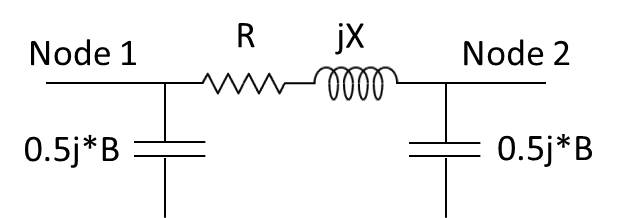
\includegraphics[width=3.2in,height= 1.14in]{PowerGridBranch.jpg}}
  \caption[Lumped $\Pi$ Model for PowerGridBranch]{Lumped $\Pi$ Model for PowerGridBranch. \label{figPowerGridBranch}}
\end{figure}
The Y-Matrix for the \texttt{PowerGridBusShunt} device can be expressed as follows where 
$G$ is the bus shunt conductance and $B$ is the bus shunt susceptance given
on the device's instance line:

\begin{equation}
  \left[ \begin{array}{cc} 
         Y_{11} & Y_{12} \\ Y_{21} & Y_{22} \\  
         \end{array} \right] =
  \left[ \begin{array}{cc} 
         g_{11}+jb_{11} & g_{12}+jb_{12} \\  g_{21}+jb_{21} & g_{22}+jb_{22}
         \end{array} \right] =
  \left[ \begin{array}{cc} 
         G+jB & -G-jB \\ -G-jB & G+jB
         \end{array} \right]
\end{equation}
% Model for PowerGridBusShunt
\begin{figure}[ht]
  \centering
  \scalebox{1.0}
  {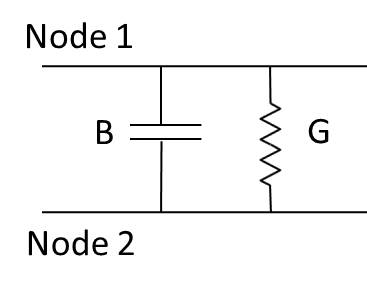
\includegraphics[width=1.91in,height= 1.43in]{PowerGridBusShunt.jpg}}
  \caption[Equivalent Circuit for PowerGridbusShunt]{Equivalent Circuit for PowerGridBusShunt. \label{figPowerGridBusShunt}}
\end{figure}
\paragraph{Equations Common to Power Grid Branch and Bus Shunt}
The \texttt{PowerGridBranch} and \texttt{PowerGridBusShunt} devices use the same
basic equations to model voltage and current flow or voltage and power flow. The 
differences are in the Y-Matrices described above.  There are three options for 
the equations used, namely I=YV, PQ Polar and PQ Rectangular.

For the I=YV format, the device equations for the \texttt{PowerGridBranch} and 
\texttt{PowerGridBusShunt} devices are as follows, where the $g_{ij}$ and $b_{ij}$ 
terms are given above.  Also, $V_{R1}$ and $V_{I1}$ are the real and imaginary parts 
of the voltage at terminal 1.  $I_{R1}$ and $I_{I1}$ are the real and imaginary parts 
of the current at terminal 1.

\begin{equation}
  \left[ \begin{array}{c} I_{R1} \\ I_{R2} \\ I_{I1} \\ I_{I2} 
         \end{array} \right] =
  \left[ \begin{array}{cccc}
      g_{11} & g_{12} & -b_{11} & -b_{12} \\
      g_{21} & g_{22} & -b_{21} & -b_{22} \\
      b_{11} & b_{12} & g_{11} & g_{12} \\
      b_{21} & b_{22} & g_{21} & g_{22} \\
      \end{array} \right] 
  \left[ \begin{array}{c} V_{R1} \\ V_{R2} \\ V_{I1} \\ V_{I2}
         \end{array} \right]
\end{equation}

For the PQ Rectangular format, the device equations are nonlinear ~\cite{Milano}.
\begin{eqnarray}
  P_{1} = g_{11}(V_{R1}^{2} + V_{I1}^{2}) + V_{R1}(g_{12}*V_{R2}-b_{12}*V_{I2})
         + V_{I1}(b_{12}*V_{R2}+g_{12}*V_{I2})\\ 
  P_{2} = g_{22}(V_{R2}^{2} + V_{I2}^{2}) + V_{R2}(g_{21}*V_{R1}-b_{21}*V_{I1})
         + V_{I2}(b_{21}*V_{R1}+g_{21}*V_{I1})\\ 
  Q_{1} = -b_{11}(V_{R1}^{2} + V_{I1}^{2}) + V_{I1}(g_{12}*V_{R2}-b_{12}*V_{I2})
         + V_{R1}(b_{12}*V_{R2}+g_{12}*V_{I2})\\  
  Q_{2} = -b_{22}(V_{R2}^{2} + V_{I2}^{2}) + V_{I2}(g_{21}*V_{R1}-b_{21}*V_{I1})
         + V_{R2}(b_{21}*V_{R1}+g_{21}*V_{I1})
\end{eqnarray}

For the PQ Polar format, the device equations are also nonlinear ~\cite{Milano}. 
Define $|V_{1}|$ as the voltage magnitude at terminal 1 and $\Theta_{1}$ as the 
voltage angle at terminal 1.
\begin{eqnarray}
  P_{1} = g_{11} * |V_{1}|^{2} 
        + |V_{1}| * |V_{2}| * (g_{12}*cos(\Theta_{1}-\Theta_{2}) + b_{12}*sin(\Theta_{1}-\Theta_{2}))\\ 
  P_{2} = g_{22} * |V_{2}|^{2} 
        + |V_{2}| * |V_{1}| * (g_{21}*cos(\Theta_{2}-\Theta_{1}) + b_{21}*sin(\Theta_{2}-\Theta_{1}))\\ 
  Q_{1} =  -b_{11} * |V_{1}|^{2} 
        + |V_{1}| * |V_{2}| * (g_{12}*sin(\Theta_{1}-\Theta_{2}) - b_{12}*cos(\Theta_{1}-\Theta_{2}))\\ 
  Q_{2} =  -b_{22} * |V_{2}|^{2} 
        + |V_{2}| * |V_{1}| * (g_{21}*sin(\Theta_{2}-\Theta_{1}) - b_{21}*cos(\Theta_{2}-\Theta_{1}))
\end{eqnarray}

\paragraph{Equations for Power Grid Transformer}
The equations for the PowerGridTransformer device are similar to those used by the 
PowerGridBranch and PowerGridBusShunt devices.  The circuit diagram for the
PowerGridTransformer is shown below.

For I=YV and PQ Rectangular formats, the equations are the same as for the \texttt{PowerGridBranch}
and \texttt{PowerBusBusShunt} devices.  However, the following Y-Matrix is used where
where $A=(R+jX)^{-1}$, $R$ is the resistance, $X$ is the reactance, $n$ is the turns ratio (which is
the \texttt{TR} instance parameter) and $\phi$ is the phase shift in radians (which is 
the \texttt{PS} instance parameter).

For the I=YV and PQ Rectangular formats, the Y matrix is not symmetric and is given by the following
\cite{Kundur}. Let the effective complex turns ratio be $r = m + jp = n*(cos(\phi) + j*sin(\phi))$:

\begin{equation}
  \left[ \begin{array}{cc} 
         Y_{11} & Y_{12} \\ Y_{21} & Y_{22} \\  
         \end{array} \right] =
  \left[ \begin{array}{cc} 
         g_{11}+jb_{11} & g_{12}+jb_{12} \\  g_{21}+jb_{21} & g_{22}+jb_{22}
         \end{array} \right] =
  \left[ \begin{array}{cc} 
         A*(m^{2}+p^{2})^{-1} & -A*(m-jp)^{-1} \\ -A*(m+jp)^{-1} & A
         \end{array} \right]
\end{equation}

The voltage-current and power flow equations for the I=YV and PQ Rectangular formats
are then the same as for the \texttt{PowerGridBranch}
and \texttt{PowerGridBusShunt} devices, with the modified Y-matrix parameters given above.

For the PQ Polar format, the Y matrix is not symmetric and is given by ~\cite{Milano}:

\begin{equation}
  \left[ \begin{array}{cc} 
         Y_{11} & Y_{12} \\ Y_{21} & Y_{22} \\  
         \end{array} \right] =
  \left[ \begin{array}{cc} 
         g_{11}+jb_{11} & g_{12}+jb_{12} \\  g_{21}+jb_{21} & g_{22}+jb_{22}
         \end{array} \right] =
  \left[ \begin{array}{cc} 
         A*n^{-2} & -A*n^{-1} \\ -A*n^{-1} & A
         \end{array} \right]
\end{equation}
% Model for PowerGridBranch
\begin{figure}[ht]
  \centering
  \scalebox{1.0}
  {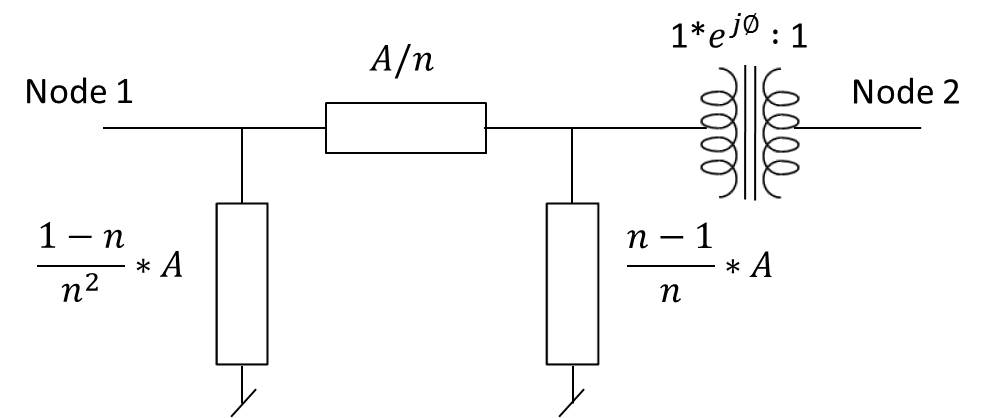
\includegraphics[width=5.17in,height= 2.21in]{PowerGridTransformer.jpg}}
  \caption[Equivalent Circuit for PowerGridTransformer]{Equivalent Circuit for PowerGridTransformer. \label{figPowerGridTransformer}}
\end{figure}
The power flow equation for PQ Polar format are then:
\begin{eqnarray}
  P_{1} = g_{11} * |V_{1}|^{2} 
        + |V_{1}| * |V_{2}| * (g_{12}*cos(\Theta_{1}-\Theta_{2}-\phi) 
                            + b_{12}*sin(\Theta_{1}-\Theta_{2}-\phi))\\ 
  P_{2} = g_{22} * |V_{2}|^{2} 
        + |V_{2}| * |V_{1}| * (g_{21}*cos(\Theta_{2}-\Theta_{1}+\phi) 
                            + b_{21}*sin(\Theta_{2}-\Theta_{1}+\phi))\\ 
  Q_{1} =  -b_{11} * |V_{1}|^{2} 
        + |V_{1}| * |V_{2}| * (g_{12}*sin(\Theta_{1}-\Theta_{2}-\phi) 
                            - b_{12}*cos(\Theta_{1}-\Theta_{2}-\phi))\\ 
  Q_{2} =  -b_{22} * |V_{2}|^{2} 
        + |V_{2}| * |V_{1}| * (g_{21}*sin(\Theta_{2}-\Theta_{1}+\phi) 
                             - b_{21}*cos(\Theta_{2}-\Theta_{1}+\phi))
\end{eqnarray}

\paragraph{Equations for Power Grid Gen Bus}
The \texttt{PowerGridGenBus} is an active device that functions as an ideal generator 
with a fixed power output ($P$) and voltage magnitude ($VM$).  Reactive power 
(\texttt{QMAX} and \texttt{QMIN}) limits are also supported.  The device equations
for the PQ Polar format are as follows ~\cite{Milano}.  The other solution formulations are 
not supported in this release.  If reactive power limits are not being enforced then:
\begin{eqnarray}
P_{1} = P \\|V_{1}| = VM
\end{eqnarray}
If reactive power limits are being enforced then $P_{1}$ is still held constant but the behavior
of the $V_{1}$ terminal changes between a constant-voltage and a constant-current source.
In particular, $|V_{1}| = VM$ only if \texttt{QMIN} $< Q_{1} <$ \texttt{QMAX}.  Otherwise, 
$|V_{1}|$ is unconstrained and the appropriate \texttt{QMIN} or \texttt{QMAX} value is 
enforced at the $V_{1}$ terminal instead.

The convention for Power Grids is that positive power is injected into the grid.
So, positive real (P) and reactive power (Q) flow out of the positive terminals 
(\texttt{inputNode 1} and \texttt{inputNode 2}).  This is reversed from the normal
convention for current direction for voltage and current sources in either \Xyce{} 
or SPICE.


%%
%% Anti-Windup Limiter device Subsection
%\clearpage
%\subsection{Anti-Windup Limiter}
%\index{anti-windup limiter}
%% Sandia National Laboratories is a multimission laboratory managed and
% operated by National Technology & Engineering Solutions of Sandia, LLC, a
% wholly owned subsidiary of Honeywell International Inc., for the U.S.
% Department of Energy’s National Nuclear Security Administration under
% contract DE-NA0003525.

% Copyright 2002-2020 National Technology & Engineering Solutions of Sandia,
% LLC (NTESS).

 
The simulation of control systems, such as those used in power grids,
may require two different types of limiters for ``hard limits''.  They
are known as ``windup'' and ``anti-windup'' limiters ~\cite{Milano},
and are typically depicted as shown in Figures \ref{figAntiWindupLimiter} 
and \ref{figWindupLimiter}. The anti-windup limiter has the following 
equations:
\[
  \begin{array}{ll} 
  \mbox{if} \; x \geq x^{max} \; \mbox{and} \; \dot{x} \geq 0 \Rightarrow x = x^{max} \; \mbox{and} \; \dot{x} = 0\\
  \mbox{if} \; x \leq x^{min} \; \mbox{and} \; \dot{x} \leq 0 \Rightarrow x = x^{min} \; \mbox{and} \; \dot{x} = 0\\
  \mbox{otherwise} \; x = (y-x)/T
  \end{array}
\]
The anti-windup limiter has simultaneous constraints on both the output-voltage
level and the first derivative of the output-voltage level.  These equations were 
approximated with a \Xyce{} device model, as described below.  

\begin{figure}[ht]
  \centering
  \scalebox{1.0}
  {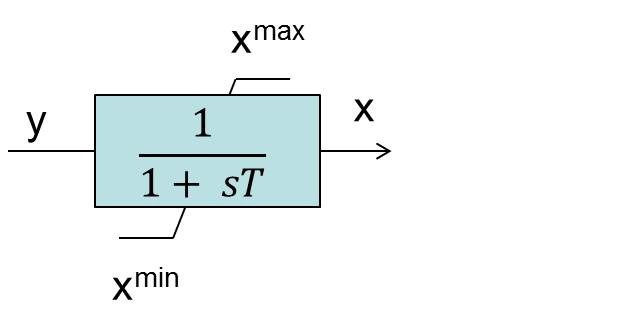
\includegraphics[width=2.1in,height= 1.05in]{AntiWindupLimiter.jpg}}
  \caption[Anti-Windup Limiter]{Anti-Windup Limiter. \label{figAntiWindupLimiter}}
\end{figure}

The windup limiter only has a constraint on the output-voltage level.  This is 
straightforward to implement with existing \Xyce{} device models.  The equations
and an example implementation are given below after the description of the \Xyce{} 
anti-windup limiter device model.

\begin{figure}[ht]
  \centering
  \scalebox{1.0}
  {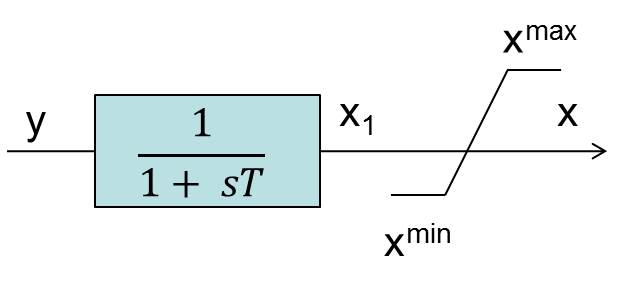
\includegraphics[width=2.0in,height= 1.0in]{WindupLimiter.jpg}}
  \caption[Windup Limiter]{Windup Limiter. \label{figWindupLimiter}}
\end{figure}

\begin{Device}\label{AntiWindupLimiter}

\device
\begin{alltt}
Y<type> <name> <input node> <output node> [device parameters] 
\end{alltt}
  
\examples
\begin{alltt}
YAntiWindupLimiter awl1 in1 out1 T=1 UL=0.5 LL=-0.5
YAWL awl2 in2 out2 T=2 UL=0.5 LL=-0.5
\end{alltt}

\parameters 
\begin{Parameters}
\param{type}
The device type has a verbose (\texttt{AntiWindupLimiter}) and a shortened
(\texttt{AWL}) form.  Their usage may be mixed within a netlist.

\param{name}
Name of the device instance.  This must be present, and unique amongst the 
\texttt{AntiWindupLimiter} devices in the netlist.

\param{input node}
There is one input node, \texttt{<input node>}. 

\param{output node}
There is one output node, \texttt{<output node>}.

\param{T} 
The time-constant, in seconds. 

\param{UL}
The upper control limit, in per-unit. The upper control limit must be 
greater than the lower control limit.  For numerical stability reasons,
the output signal level may exceed this upper limit slightly, depending 
on the time-steps used by \Xyce{}. The reason is that the derivative of 
the AWL output must be continuous in the current implementation of this 
device model.

\param{LL}
The lower control limit, in per-unit. For numerical stability reasons,
the output signal level may be slightly less than this lower limit, depending 
on the time-steps used by \Xyce{}. The reason is that the derivative of 
the AWL output must be continuous in the current implementation of this 
device model.
\end{Parameters}
\end{Device}

\paragraph{Anti-Windup Limiter Device Parameters}
%%
%% AntiWindupLimiter Table
%%
% This table was generated by Xyce:
%   Xyce -doc AntiWindupLimiter 1
%
\index{antiwinduplimiter!device instance parameters}
\begin{DeviceParamTableGenerated}{AntiWindupLimiter Device Instance Parameters}{AntiWindupLimiter_1_Device_Instance_Params}
LL & Lower Limit & per unit & -1 \\ \hline
T & Time Constant & s & 1 \\ \hline
UL & Upper Limit & per unit & 1 \\ \hline
\end{DeviceParamTableGenerated}



\paragraph{Branch Current and Power Accessors}
This version of the Anti-Windup Limiter device does not 
support the branch current accessor, \texttt{I()}, 
or the power accessors, \texttt{P()} or \texttt{W()}.

\paragraph{Comments}
The model parameters \texttt{UL} and \texttt{LL} are specified 
in ``per-unit'' since the AWL device was developed
for use with the power grid devices.  For other uses, the upper
and lower control limits can be considered to be specified in 
volts.

\paragraph{Windup Limiter}
For a first-order low-pass filter, followed by a hard-limiting function,
the windup limiter has the following equations and can be depicted
as shown in Figure \ref{figWindupLimiter}:
\[
x = \left\{ \begin{array}{ll}
x^{max}, &  \mbox{if} \; x_{1} \geq x^{max}\\
x, &  \mbox{if} \; x^{min} < x_{1} < x^{max}\\
x^{min}, & \mbox{if} \; x_{1} \leq x^{min}
\end{array}
\right.
\]
The version of the windup limiter shown in Figure \ref{figWindupLimiter}
can be implemented as a first-order RC filter followed by a B-Source with
a \texttt{LIMIT} function.  An example \Xyce{} netlist fragment is as follows:
\begin{alltt}
.param timeConstant=1
.param upperLimit=0.5
.param lowerLimit=-0.5
Rlpf y x1 {timeConstant}
Clpf x1 0 1
BLim x 0 V={LIMIT(V(x1),lowerLimit,upperLimit)}
\end{alltt}


%%
%% Memristor Device subsection
%%
\clearpage
\subsection{Memristor Device}
\index{memristor}
% Sandia National Laboratories is a multimission laboratory managed and
% operated by National Technology & Engineering Solutions of Sandia, LLC, a
% wholly owned subsidiary of Honeywell International Inc., for the U.S.
% Department of Energy’s National Nuclear Security Administration under
% contract DE-NA0003525.

% Copyright 2002-2022 National Technology & Engineering Solutions of Sandia,
% LLC (NTESS).


\begin{Device}

\symbol
{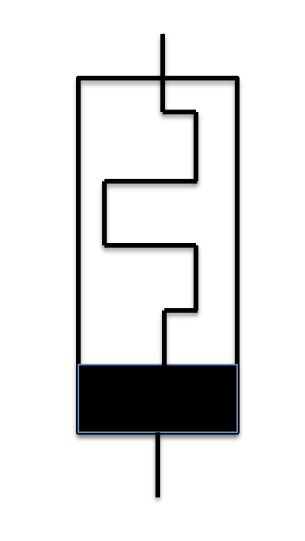
\includegraphics[scale=.2, angle=90]{MemristorSymbol}}

\device
ymemristor <name> <(+) node> <(-) node> <model>

\model
\begin{alltt}
.MODEL <model name> MEMRISTOR level=2 [model parameters]
\end{alltt}

\examples
\begin{alltt}

ymemristor mr1 n1 n2 mrm2

.model mrm2 memristor level=2 ron=50 roff=1000 
+ koff=1.46e-18 kon=-4.68e-22 
+ alphaoff=10 alphaon=10 wc=1.0e-12 
+ ioff=115e-6 ion=-8.9e-6 xscaling=1.0e9 wt=4


ymemristor mr2 n1 n2 mrm3 xo=0.11 

.MODEL mrm3 memristor level=3 a1=0.17 a2=0.17 b=0.05 vp=0.16 vn=0.15 
+ ap=4000 an=4000 xp=0.3 xn=0.5 alphap=1 alphan=5 eta=1 


ymemristor mr3 n1 n2 mrm4 

.model mrm4 memristor level=4 
+ fxpdata=fxp_table.csv
+ fxmdata=fxm_table.csv
+ I1=85.37e-6 I2=90.16e-6 V1=0.265 V2=0.265 G0=130.72e-6
+ VP=0.7 VN=1.0 d1=9.87 d2=-4.82
+ C1=1000 C2=1000

\end{alltt}

\parameters

\begin{Parameters}
\param{\vbox{\hbox{(+) node\hfil}\hbox{(-) node}}}

Polarity definition for a positive voltage across the memristor. The
first node is defined as positive. Therefore, the voltage across the
component is the first node voltage minus the second node voltage.


\end{Parameters}

\comments
The {\tt level=2} memristor device is an implementation of the TEAM formulation described 
in~\cite{KvatinskyFriedman2012} and~\cite{KvatinskyFriedman2013}.
The {\tt level=3}  memristor device is an implementation of the Yakopcic formulation described 
in~\cite{ChrisYakopcic2013}. The {\tt level=4} memristor device is an implementation of the 
Piecewise Empirical Model described in~\cite{Niroula2017}.

Positive current flows from
the \texttt{(+)} node through the device to the \texttt{(-)}
node. The power through the device is calculated 
with $I \cdot \Delta V$ where the voltage drop is calculated as $(V_+ - V_-)$ 
and positive current flows from $V_+$ to $V_-$.  
\end{Device}

\paragraph{Device Equations for TEAM Formulation}
The current voltage relationship for the TEAM formulation can be linear or nonlinear and this is selectable with 
the instance parameter {\tt IVRELATION}.  The default is the linear relationship which is:
\begin{equation}
v(t) = \left[ R_{ON} + \frac{R_{OFF} - R_{ON}}{x_{OFF} - x_{ON}} \left( x - x_{ON} \right) \right] i(t)
\end{equation}
The non-linear relationship is:
\begin{equation}
v(t) = R_{ON} e^{\lambda(x - x_{ON})/(x_{OFF}-x_{ON})}  i(t)
\end{equation}
where $\lambda$ is defined as:
\begin{equation}
\frac{R_{OFF}}{R_{ON}} = e^{\lambda}
\end{equation}
In the above equations $x$ represents a doped layer whose growth determines the overall
resistance of the device.  The equation governing the value of $x$ is:
\begin{equation}
\frac{dx}{dt} = \left\{  
  \begin{array}{ll}
    k_{OFF} \left(\frac{i}{i_{OFF}} - 1 \right)^{\alpha_{OFF}} f_{OFF}(x) & 0 < i_{OFF} < i \\
    0       & i_{ON} < i < i_{OFF} \\
    k_{ON} \left(\frac{i}{i_{on}} - 1 \right)^{\alpha_{on}} f_{ON}(x) & i < i_{ON} < 0 \\
  \end{array}
  \right.
\end{equation}

The functions $f_{ON}(x)$ and $f_{OFF}(x)$ are window functions designed to keep $x$ within
the defined limits of $x_{ON}$ and $x_{OFF}$.  Four different types of window functions 
are available and this is selectable with the model parameter {\tt WT}. Note that the 
TEAM memristor device is formulated to work best with the TEAM, Kvatinsky, window 
function {\tt WT=4 }.  Other window functions should be used with caution.

\paragraph{Device Equations for Yakopcic Formulation}
The current voltage relationship for the Yakopcic memristor device is:~\cite{ChrisYakopcic2013}
\begin{equation}
I(t) = \left\{  
  \begin{array}{ll}
    a_1 x(t) \sinh(b V(t)) & V(t) \ge 0 \\
    a_2 x(t) \sinh(b V(t)) & V(t) < 0 \\
  \end{array}
  \right.
\end{equation}

\begin{equation}
g(V(t)) = \left\{  
  \begin{array}{ll}
    A_p\left( \exp^{V(t)} - \exp^{V_p}\right) & V(t) > V_p \\
    -A_n \left( \exp^{-V(t)} - \exp^{V_n}\right) & V(t) < -V_n \\
    0       & -V_n \le V(t) \le V_p \\
  \end{array}
  \right.
\end{equation}

The internal state variable, $x$, is governed by the equation:

\begin{equation}
\frac{dx}{dt} = n g(V(t)) f(x(t))
\end{equation}

where $f(x)$ is defined by:

\begin{equation}
f(x) = \left\{  
  \begin{array}{ll}
   \exp^{-\alpha_p (x-x_p)} w_p(x,x_p) & x \ge x_p \\
   1 & x \le x_p \\
  \end{array}
  \right.
\end{equation}
\begin{equation}
f(x) = \left\{  
  \begin{array}{ll}
   \exp^{\alpha_n (x+x_n-1} w_n(x,x_n) & x \le 1-x_n \\
   1 & x > 1 - x_n \\
  \end{array}
  \right.
\end{equation}
\begin{equation}
w_p(x,x_p) = \frac{x_p -x}{1 - x_p} + 1
\end{equation}
\begin{equation}
w_n(x,x_n) = \frac{x}{1-x_n}
\end{equation}

Note, the quantities, $x_p$, $x_n$, $\alpha_p$, $\alpha_n$, $A_p$, $A_n$, $a_1$, $a_2$ and$b$ are model
parameters that can be specified in the device's model block.


\paragraph{Device Equations for the PEM Formulation}
The PEM memristor device is similar to the TEAM and Yakopcic formulations in that an 
internal state variable, $x$, is used to capture the device's response to its history.

The I-V relationship is
\begin{equation}
I = x \: h(V)
\end{equation}

and $h(V)$ is defined by:
\begin{equation}
 h(V) = I_1 * exp(V/V_1) - I_2 * exp(-V/V_2) + G_0 V - (I_1-I_2)
\end{equation}
where $I_1$, $I_2$, $V_1$, $V_2$ and $G_0$ are model parameters.

The internal variable, $x$, is defined by:
\begin{equation}
  \frac{dx}{dt} = G(V) f(x)
\end{equation}
with
\begin{equation}
G(V) = \left\{  
  \begin{array}{ll}
   C_1 \left( \exp^{d_1\left[ V(t) - V_p\right]} - 1\right) & V > V_p \\
   C_2 \left( \exp^{d_2\left[ V(t) - V_n\right]} - 1\right) & V < -V_n \\
   0 & -V_n \le V(t) \le V_p \\
  \end{array}
  \right.
\end{equation}

Finally, the function $f(x)$ is defined by a user supplied set set data which is 
used with linear interpolation to find the current value of $f(x)$.  Separate data
sets are used for forward bias and reverse bias.
\begin{equation}
f(x) = \left\{  
  \begin{array}{ll}
   F^+ {\tt data set} & V > 0 \\
   F^- {\tt data set} & V < 0 \\
  \end{array}
  \right.
\end{equation}




%%\pagebreak

\paragraph{Device Parameters for TEAM Formulation}
% This table was generated by Xyce:
%   Xyce -doc Memristor 2
%
\index{memristorteam!device instance parameters}
\begin{DeviceParamTableGenerated}{MemristorTEAM Device Instance Parameters}{Memristor_2_Device_Instance_Params}
IVRELATION & IV relationship to use, 0 is linear, 1 is nonlinear & -- & 0 \\ \hline
\end{DeviceParamTableGenerated}


\paragraph{Model Parameters for TEAM Formulation}
% This table was generated by Xyce:
%   Xyce -doc Memristor 2
%
\index{memristorteam!device model parameters}
\begin{DeviceParamTableGenerated}{MemristorTEAM Device Model Parameters}{Memristor_2_Device_Model_Params}
ALPHAOFF & Modeling Coefficient & -- & 3 \\ \hline
ALPHAON & Modeling Coefficient & -- & 3 \\ \hline
AOFF & Window Function Parameter (window 4) & m & 3e-09 \\ \hline
AON & Window Function Parameter (window 4) & m & 0 \\ \hline
D & Window Function Parameter (windows 1, 2 and 3) & -- & 0.000115 \\ \hline
IOFF & Current scale in off state & $\mathsf{\Omega}$ & 0.000115 \\ \hline
ION & Current scale in On state & A & 8.9e-06 \\ \hline
J & Window Function Parameter (window 3) & -- & 0.000115 \\ \hline
KOFF & Modeling Coefficient & m/s & 8e-13 \\ \hline
KON & Modeling Coefficient & m/s & -8e-13 \\ \hline
P & Window Function Parameter (windows 1, 2 and 3) & -- & 0.000115 \\ \hline
ROFF & Resistence in off state & $\mathsf{\Omega}$ & 1000 \\ \hline
RON & Resistence in on state & $\mathsf{\Omega}$ & 50 \\ \hline
WC & Window Function Parameter (window 4) & m & 1.07e-12 \\ \hline
WT & Type of windowing function: 0-None, 1-Jogelkar, 2-Biolek, 3-Prodromakis, 4-Kvatinsky & -- & 0 \\ \hline
XOFF & Modeling Coefficient & m & 3e-09 \\ \hline
XON & Modeling Coefficient & m & 0 \\ \hline
XSCALING & Scaling for x variable.  For example 1e9 if x will be in units of nanometers. & -- & 1 \\ \hline
\end{DeviceParamTableGenerated}




% Sandia National Laboratories is a multimission laboratory managed and
% operated by National Technology & Engineering Solutions of Sandia, LLC, a
% wholly owned subsidiary of Honeywell International Inc., for the U.S.
% Department of Energy’s National Nuclear Security Administration under
% contract DE-NA0003525.

% Copyright 2002-2022 National Technology & Engineering Solutions of Sandia,
% LLC (NTESS).


\paragraph{Device Parameters for Yakopcic Formulation}
% This table was generated by Xyce:
%   Xyce -doc Memristor 3
%
\index{memristoryakopcic!device instance parameters}
\begin{DeviceParamTableGenerated}{MemristorYakopcic Device Instance Parameters}{Memristor_3_Device_Instance_Params}
XO & Initial value for internal variable x & -- & 0 \\ \hline
\end{DeviceParamTableGenerated}


\paragraph{Model Parameters for Yakopcic Formulation}
% This table was generated by Xyce:
%   Xyce -doc Memristor 3
%
\index{memristoryakopcic!device model parameters}
\begin{DeviceParamTableGenerated}{MemristorYakopcic Device Model Parameters}{Memristor_3_Device_Model_Params}
A1 & Dielectric layer thickness parameter [dimensionless]  & -- & 1 \\ \hline
A2 & Dielectric layer thickness parameter [dimensionless]  & -- & 1 \\ \hline
ALPHAN & State variable motion. & -- & 1 \\ \hline
ALPHAP & State variable motion. & -- & 1 \\ \hline
AN & Negative Voltage Threshold Magnitude Parameter & -- & 1 \\ \hline
AP & Positive Voltage Threshold Magnitude Parameter & -- & 1 \\ \hline
B & Curvature in I-V relation.  Relates to how much conduction in the device is Ohmic and versus tunnel barrier. & -- & 1 \\ \hline
ETA & State variable motion relative to voltage. & -- & 1 \\ \hline
RESDELTA & RTN model in resistance: Base change in resistance for RTN & $\mathsf{\Omega}$ & 0 \\ \hline
RESDELTAGRAD & RTN model in resistance: Base change in resistance for RTN scaled by R & -- & 0 \\ \hline
RESEPTD & RTN model in resistance: Minimum allowed update time & s & 1e-10 \\ \hline
RESLAMBDA & RTN model: lambda & -- & 0 \\ \hline
RESNOISE & RTN model in resistance (on/off) & -- & false \\ \hline
RESSEED & RTN model in resistance: seed & -- & 0 \\ \hline
RESTD & RTN model in resistance: Update time & s & 0 \\ \hline
VN & Negative Voltage Threshold & V & -0.01 \\ \hline
VP & Positive Voltage Threshold & V & 0.01 \\ \hline
XDELTA & RTN model in growth: Base change in growth rate for RTN & $\mathsf{\Omega}$ & 0 \\ \hline
XDELTAGRAD & RTN model in growth: Base change in growth for RTN scaled by X & -- & 0 \\ \hline
XEPTD & RTN model in growth: Minimum allowed update time & s & 1e-10 \\ \hline
XLAMBDA & RTN growth model: lambda & -- & 0 \\ \hline
XN & State variable motion. & -- & 1 \\ \hline
XNOISE & RTN model in growth (on/off) & -- & false \\ \hline
XP & State variable motion. & -- & 1 \\ \hline
XSCALING & Scaling for x variable.  For example 1e9 if x will be in units of nanometers. & -- & 1 \\ \hline
XSEED & RTN model in growth: seed & -- & 0 \\ \hline
XTD & RTN model in growth: Update time & s & 0 \\ \hline
\end{DeviceParamTableGenerated}





% Sandia National Laboratories is a multimission laboratory managed and
% operated by National Technology & Engineering Solutions of Sandia, LLC, a
% wholly owned subsidiary of Honeywell International Inc., for the U.S.
% Department of Energy’s National Nuclear Security Administration under
% contract DE-NA0003525.

% Copyright 2002-2022 National Technology & Engineering Solutions of Sandia,
% LLC (NTESS).


\paragraph{Device Parameters for PEM Formulation}
% This table was generated by Xyce:
%   Xyce -doc Memristor 4
%
\index{memristorpem!device instance parameters}
\begin{DeviceParamTableGenerated}{MemristorPEM Device Instance Parameters}{Memristor_4_Device_Instance_Params}
XO & Initial value for internal variable x & -- & 0 \\ \hline
\end{DeviceParamTableGenerated}


\paragraph{Model Parameters for PEM Formulation}
% This table was generated by Xyce:
%   Xyce -doc Memristor 4
%
\index{memristorpem!device model parameters}
\begin{DeviceParamTableGenerated}{MemristorPEM Device Model Parameters}{Memristor_4_Device_Model_Params}
C1 & State variable proportionality parameter for forward bias & -- & 1 \\ \hline
C2 & State variable proportionality parameter for negative bias & -- & 1 \\ \hline
D1 & Positive Voltage Threshold Magnitude Parameter & -- & 1 \\ \hline
D2 & Negative Voltage Threshold Magnitude Parameter & -- & 1 \\ \hline
FXMDATA & File from which to read x,f-(x) data & -- & 'filem.dat' \\ \hline
FXPDATA & File from which to read x,f+(x) data & -- & 'filep.dat' \\ \hline
G0 & Conductance factor. & -- & 1 \\ \hline
I1 & Current Scale factor. & A & 1 \\ \hline
I2 & Current Scale factor. & A & 1 \\ \hline
V1 & Voltage Scale factor. & V & 1 \\ \hline
V2 & Voltage Scale factor. & V & 1 \\ \hline
VN & Negative Voltage Threshold & V & -0.01 \\ \hline
VP & Positive Voltage Threshold & V & 0.01 \\ \hline
\end{DeviceParamTableGenerated}






%%
%% Subcircuit Subsection
%%
\clearpage
\subsection{Subcircuit}
\label{SubcircuitInstance}
\index{subcircuit}
% Sandia National Laboratories is a multimission laboratory managed and
% operated by National Technology & Engineering Solutions of Sandia, LLC, a
% wholly owned subsidiary of Honeywell International Inc., for the U.S.
% Department of Energy’s National Nuclear Security Administration under
% contract DE-NA0003525.

% Copyright 2002-2020 National Technology & Engineering Solutions of Sandia,
% LLC (NTESS).


\label{XDevicesection}
A subcircuit can be introduced into the circuit netlist
using the specified nodes to substitute for the argument nodes in the
definition.  It provides a building block of circuitry to be defined a single
time and subsequently used multiple times in the overall circuit netlists.
See Section~\ref{SUBCKTsection} for more information about subcircuits.

\begin{Device}

\device
X<name> [node]* <subcircuit name> [PARAMS: [<name> = <value>]*]

\examples
\begin{alltt}
  X12 100 101 200 201 DIFFAMP
  XBUFF 13 15 UNITAMP
  XFOLLOW IN OUT VCC VEE OUT OPAMP
  XFELT 1 2 FILTER PARAMS: CENTER=200kHz
  XNANDI 25 28 7 MYPWR MYGND PARAMS: IO\_LEVEL=2
\end{alltt}

\parameters

\begin{Parameters}

\param{subcircuit name}
The name of the subcircuit's definition.

\param{PARAMS:}

Passed into subcircuits as arguments and into expressions inside the
subcircuit.

\end{Parameters}

\comments

There must be an equal number of nodes in the subcircuit call and in its
definition.

Subcircuit references may be nested to any level. However, the nesting
cannot be circular. For example, if subcircuit \texttt{A}'s definition
includes a call to subcircuit \texttt{B}, then subcircuit \texttt{B}'s
definition cannot include a call to subcircuit \texttt{A}.

\end{Device}


%%

%%% Local Variables:
%%% mode: latex
%%% End:

% END of Xyce_RG_app1.tex ************

\cleardoublepage
% Sandia National Laboratories is a multimission laboratory managed and
% operated by National Technology & Engineering Solutions of Sandia, LLC, a
% wholly owned subsidiary of Honeywell International Inc., for the U.S.
% Department of Energy’s National Nuclear Security Administration under
% contract DE-NA0003525.

% Copyright 2002-2019 National Technology & Engineering Solutions of Sandia,
% LLC (NTESS).


%%-------------------------------------------------------------------------
%% Purpose        : Main LaTeX Xyce Reference Guide
%% Special Notes  : Graphic files (pdf format) work with pdflatex.  To use
%%                  LaTeX, we need to use postcript versions.
%% Creator        : Eric R. Keiter, Computational Sciences, SNL
%% Creation Date  : {01/26/2003}
%%
%%-------------------------------------------------------------------------

%%
%% PDE Device simulation/TCAD Device Simulation.
%%
\clearpage
\section{TCAD Devices}
\index{device!PDE Devices}\index{PDE Devices}\index{TCAD Devices}
% Sandia National Laboratories is a multimission laboratory managed and
% operated by National Technology & Engineering Solutions of Sandia, LLC, a
% wholly owned subsidiary of Honeywell International Inc., for the U.S.
% Department of Energy’s National Nuclear Security Administration under
% contract DE-NA0003525.

% Copyright 2002-2020 National Technology & Engineering Solutions of Sandia,
% LLC (NTESS).


Semiconductor device simulation, which is based on a coupled set of partial
differential equations (PDE's) is supported in \Xyce{}.  Such devices can be
invoked from the circuit netlist in a manner similar to traditional SPICE-style
analog devices.  One dimensional and two dimensional devices are supported,
with the dimensionality determined by the device model level.

\begin{Device}

\item[1D Device Form]
\begin{alltt}
YPDE <name> <node> [node] [model name]
+ [device parameters]
\end{alltt}

\vbox{\hrulefill}
\item[2D Device Form]
\begin{alltt}
YPDE <name> <node> <node> [node][node] [model name]|
+ [device parameters]
\end{alltt}

\model
\begin{alltt}
.MODEL <model name> ZOD [model parameters]
\end{alltt}

\comments

All of the PDE parameters are specified on the instance level.  The model
statement is used only for specifying if the device is 1D or 2D, via the level
parameter.  Both the 1D and the 2D devices can construct evenly-spaced meshes
internally, or an unstructured mesh can be read in from an external mesh file.

The eletrode, doping and material parameters are specified using a special
format that is described in the tables that are referenced in the instance
parameter tables.
\end{Device}

\paragraph{TCAD Device Parameters}
Most TCAD device parameters are specified on the instance level.
\noindent
The only TCAD device model parameter is the level, which specifies whether the
model is one or two dimensions.

\label{PDE_Model_Params}
\index{PDE Devices!model parameters}
\begin{DeviceParamTable}{PDE Device Model Parameters}
LEVEL & Determines if the device is 1D or 2D  1=1D, 2=2D & -- & 1 \\ \hline
\end{DeviceParamTable}

\index{PDE Devices!1D instance parameters}
% This table was generated by Xyce:
%   Xyce -doc_cat Pde 1
%
\index{1d pde (level 1)!device instance parameters}
\begin{DeviceParamTableGenerated}{1D PDE (level 1) Device Instance Parameters}{Pde_1_Device_Instance_Params}
AUGER & Flag to turn on/off Auger recombination & logical (T/F) & true \\ \hline
BULKMATERIAL & Bulk semiconductor material & -- & 'SI' \\ \hline
DOPINGPROFILES &  & \multicolumn{2}{c}{See Table~\ref{DOPINGPROFILES_Composite_Params}}  \\ \hline
FERMIDIRAC & Use Fermi-Dirac statistics. & logical (T/F) & false \\ \hline
FIELDDEP & If true, use field dependent mobility. & logical (T/F) & false \\ \hline
LAYER &  & \multicolumn{2}{c}{See Table~\ref{LAYER_Composite_Params}}  \\ \hline
MASKVARSTIA & If set to true, then some variables are excluded from the time integration error control calculation. & logical (T/F) & false \\ \hline
MAXVOLTDELTA & Maximum voltage change used by two-level Newton algorithm. & V & 0.025 \\ \hline
MESHFILE &  & -- & 'internal.msh' \\ \hline
MOBMODEL & Mobility model. & -- & 'ARORA' \\ \hline
NODE &  & \multicolumn{2}{c}{See Table~\ref{NODE_Composite_Params}}  \\ \hline
NX & Number of mesh points & -- & 11 \\ \hline
REGION &  & \multicolumn{2}{c}{See Table~\ref{REGION_Composite_Params}}  \\ \hline
SRH & Flag to turn on/off Shockley-Read-Hall (SRH) recombination. & logical (T/F) & true \\ \hline
THERMIONICEMISSION &  & logical (T/F) & false \\ \hline
TUNNELING &  & -- & 'none' \\ \hline
USEOLDNI & Flag for using old(inaccurate) intrinsic carrier calculation. & logical (T/F) & false \\ \hline
VOLTLIM & Flag to apply voltage limiting.  This is only relevant for an experimental two-level Newton solver. & logical (T/F) & false \\ \hline

\category{Doping Parameters}\\ \hline
DOPING\_FILE & File containing doping profile. & -- & 'NOFILE' \\ \hline
GRADED & Flag for graded junction vs. abrupt junction. – (1/true=graded, 0/false=abrupt) & logical (T/F) & false \\ \hline
NA & Acceptor doping level & cm$^{-3}$ & 1e+15 \\ \hline
ND & Donor doping level & cm$^{-3}$ & 1e+15 \\ \hline
NDOPE\_FILE & File containing doping profile for N-type dopants. & -- & 'NOFILE' \\ \hline
PDOPE\_FILE & File containing doping profile for P-type dopants. & -- & 'NOFILE' \\ \hline
WJ & Junction width, if graded junction enabled. & cm & 0.0001 \\ \hline

\category{Geometry Parameters}\\ \hline
ANODE.AREA & Anode area (used for two-terminal devices) & cm$^{-2}$ & 0 \\ \hline
AREA & Cross sectional area of the device. & cm$^{-2}$ & 1 \\ \hline
BASE.AREA & Base area (used for three-terminal (BJT) devices) & cm$^{-2}$ & 0 \\ \hline
BASE.LOC & Location of base contact (necessary if running with three terminals). & cm & 0.0005 \\ \hline
CATHODE.AREA & Cathode area (used for two-terminal devices) & cm$^{-2}$ & 0 \\ \hline
COLLECTOR.AREA & Collector area (used for three-terminal (BJT) devices) & cm$^{-2}$ & 0 \\ \hline
EMITTER.AREA & Emitter area (used for three-terminal (BJT) devices) & cm$^{-2}$ & 0 \\ \hline
L & Device width. (Synonym with W parameter) & cm & 0.001 \\ \hline
W & Device width. (Synonym with L parameter) & cm & 0.001 \\ \hline

\category{Temperature Parameters}\\ \hline
TEMP & Device temperature & $^\circ$C & 27 \\ \hline

\category{Model Output Parameters}\\ \hline
FIRSTELECTRODEOFFSET & This is an output parameter.  It is only used if OFFSETOUTPUTVOLTAGE=true. (see description of that paramaeter & logical (T/F) & false \\ \hline
GNUPLOTLEVEL & Flag for gnuplot output.
0 - no gnuplot files.
1 - gnuplot files.
gnuplot is an open source plotting program that is usually installed on Linux systems. gnuplot files will have the *Gnu.dat suffix, and the prefix will be thename of the device instance. & -- & 1 \\ \hline
OFFSETOUTPUTVOLTAGE & This is an output parameter that determines the ``zero'' of the potential at output.  If OFFSETOUTPUTVOLTAGE=true (default) it will adjust the voltages at output so that the minimum voltage is zero. If true and also FIRSTELECTRODEOFFSET=true, then the voltage of the first electrode is the zero point.  If OFFSETOUTPUTVOLTAGE=false, the output voltage sets the intrisic Fermi level to zero.  Depending on circumstances each of these may be more or less convenient for plotting. & logical (T/F) & true \\ \hline
OUTPUTINTERVAL & Time interval for tecplot output (if tecplot is enabled). & s & 0 \\ \hline
OUTPUTNLPOISSON & Flag to determine if the results of the nonlinear Poisson calculation is included in the output files.  Normally, this calculation is used to initialize a drift-diffusion calculation and isn't of interest. & logical (T/F) & false \\ \hline
%SGPLOTLEVEL & Flag for sgplot output.
%0 - no sgplot files.
%1 - sgplot files.
%sgplot is a plotting program that comes as part of the SG Framework. sgplot files will have the *.res suffix, and the prefix will be the name of the device instance & -- & 0 \\ \hline
TECPLOTLEVEL & Setting for Tecplot output:
0 - no Tecplot files
1 - Tecplot files, each output in a separate file. 2 - Tecplot file, each outputappended to a single file.
Tecplot files will have the .dat suffix, and the prefix will be the name of the device instance & -- & 1 \\ \hline

\category{Scaling Parameters}\\ \hline
C0 & Density scalar; adjust to mitigate convergence problems.The model will do all of its scaling automatically, so it is generally not necessary to specify it manually. & cm$^{-3}$ & 1e+15 \\ \hline
DENSITYSCALARFRACTION & Fraction of the maximum doping by which density will be scaled.The model will do all of its scaling automatically, so it is generally not necessary to specify it manually. & logical (T/F) & 0.1 \\ \hline
SCALEDENSITYTOMAXDOPING & If set the density will be scaled by a fraction of the maximum doping.The model will do all of its scaling automatically, so it is generally not necessary to specify it manually. & logical (T/F) & true \\ \hline
t0 & Time scalar; adjust to mitigate convergence problems.The model will do all of its scaling automatically, so it is generally not necessary to specify it manually. & s & 1e-06 \\ \hline
X0 & Length scalar; adjust to mitigate convergence problems.The model will do all of its scaling automatically, so it is generally not necessary to specify it manually. & cm & 1e-07 \\ \hline

\category{Boundary Condition Parameters}\\ \hline
ANODE.BC & Anode voltage boundary condition.  Only used if device is uncoupled from circuit, and running in diode mode.
 & V & 0.5 \\ \hline
BASE.BC & Base voltage boundary condition.  Only used if device is uncoupled from circuit, and running in BJT mode.
 & V & 0 \\ \hline
CATHODE.BC & Cathode voltage boundary condition.  Only used if device is uncoupled from circuit, and running in diode mode.
 & V & 0 \\ \hline
COLLECTOR.BC & Collector voltage boundary condition.  Only used if device is uncoupled from circuit, and running in BJT mode.
 & V & 0 \\ \hline
EMITTER.BC & Emitter voltage boundary condition.  Only used if device is uncoupled from circuit, and running in BJT mode.
 & V & 0.5 \\ \hline
\end{DeviceParamTableGenerated}

\clearpage

\index{PDE Devices!1D instance parameters}
% This table was generated by Xyce:
%   Xyce -doc_cat Pde 2
%
\index{2d pde (level 2)!device instance parameters}
\begin{DeviceParamTableGenerated}{2D PDE (level 2) Device Instance Parameters}{Pde_2_Device_Instance_Params}
BULKMATERIAL & Material of bulk material. & -- & 'SI' \\ \hline
DISPLCUR & If true, displacement current is computed and output & logical (T/F) & false \\ \hline
DOPINGPROFILES &  & \multicolumn{2}{c}{See Table~\ref{DOPINGPROFILES_Composite_Params}}  \\ \hline
MAXVOLTDELTA & Maximum voltage change used by two-level Newton algorithm. & V & 0.025 \\ \hline
MESHFILE & This is a required field for a 2D simulation.  If the userspecifies meshfile=internal.mesh, the model will create aCartesian mesh using the parameters L,W,NX and NY.  If the user specifies anything else (for example meshfile=diode.msh), the model will attempt to read in a mesh file of that name.  The format is assumed to be that of the SG Framework. & -- & 'internal.msh' \\ \hline
MOBMODEL & Mobility model. & -- & 'ARORA' \\ \hline
NODE &  & \multicolumn{2}{c}{See Table~\ref{NODE_2D_Composite_Params}}  \\ \hline
NX & Number of mesh points, x-direction. & -- & 11 \\ \hline
NY & Number of mesh points, y-direction. & -- & 11 \\ \hline
REGION &  & \multicolumn{2}{c}{See Table~\ref{REGION_Composite_Params}}  \\ \hline
TYPE & P-type or N-type - this is only relevant if using the default dopings & -- & 'PNP' \\ \hline
USEMATRIXGID &  & -- & false \\ \hline
USEOLDNI & Flag for using old (inaccurate) intrinsic carrier calculation. & logical (T/F) & false \\ \hline
USEVECTORGID &  & -- & false \\ \hline
VOLTLIM &  & logical (T/F) & false \\ \hline

\category{Doping Parameters}\\ \hline
GRADED & Flag for graded junction vs. abrupt junction. – (1/true=graded, 0/false=abrupt) & logical (T/F) & false \\ \hline
NA & Acceptor doping level & cm$^{-3}$ & 1e+15 \\ \hline
ND & Donor doping level & cm$^{-3}$ & 1e+15 \\ \hline
WJ & Junction width, if graded junction enabled. & cm & 0.0001 \\ \hline

\category{Geometry Parameters}\\ \hline
AREA & Cross sectional area of the device. & cm$^{-2}$ & 1 \\ \hline
CYL & Flag to enable cylindrical geometry & logical (T/F) & false \\ \hline
L & Device length & cm & 0.001 \\ \hline
W & Device width & cm & 0.001 \\ \hline

\category{Temperature Parameters}\\ \hline
TEMP & Device temperature & $^\circ$C & 27 \\ \hline

\category{Model Output Parameters}\\ \hline
GNUPLOTLEVEL & Flag for gnuplot output.
0 - no gnuplot files.
1 - gnuplot files.
gnuplot is an open source plotting program that is usually installed on Linux systems. gnuplot files will have the *Gnu.dat suffix, and the prefix will be thename of the device instance. & -- & 0 \\ \hline
INTERPGRIDSIZE &  & -- & 20 \\ \hline
OUTPUTINTERVAL & Time interval for tecplot output (if tecplot is enabled). & s & 0 \\ \hline
OUTPUTNLPOISSON & Flag to determine if the results of the nonlinear Poisson calculation is included in the output files.  Normally, this calculation is used to initialize a drift-diffusion calculation and isn't of interest. & logical (T/F) & false \\ \hline
%SGPLOTLEVEL & Flag for sgplot output.
%0 - no sgplot files.
%1 - sgplot files.
%sgplot is a plotting program that comes as part of the SG Framework. sgplot files will have the *.res suffix, and the prefix will be the name of the device instance & -- & 0 \\ \hline
TECPLOTLEVEL & Setting for Tecplot output:
0 - no Tecplot files
1 - Tecplot files, each output in a separate file. 2 - Tecplot file, each outputappended to a single file.
Tecplot files will have the .dat suffix, and the prefix will be the name of the device instance & -- & 1 \\ \hline
TXTDATALEVEL & Flag for volume-averaged text output.
0 - no text files.
1 - text files.
txtdataplot files will have the *.txt suffix, and the prefix will be the name of the device instance. & -- & 1 \\ \hline

\category{Scaling Parameters}\\ \hline
X0 & Length scalar; adjust to mitigate convergence problems. The model will do all of its scaling automatically, so it is generally not necessary to specify it manually. & cm & 0.0001 \\ \hline

\category{Boundary Condition Parameters}\\ \hline
CONSTBOUNDARY &  & -- & false \\ \hline
\end{DeviceParamTableGenerated}

\clearpage

\paragraph{Layer Parameters}
% This table was generated by Xyce
\index{layer!composite parameters}
\begin{CompositeParamTableGenerated}{LAYER Composite Parameters}{LAYER_Composite_Params}
CON &  & -- & 1.42248 \\ \hline
ConductionBandDOS &  & -- & 2.89e+19 \\ \hline
DIEL &  & -- & 13.1 \\ \hline
ELMOB0 &  & -- & 2240 \\ \hline
ELVSAT &  & -- & 7.7e+06 \\ \hline
EMASS &  & -- & 0.067 \\ \hline
GRADEDWIDTH &  & -- & 0 \\ \hline
HMASS &  & -- & 0.5 \\ \hline
HOMOB0 &  & -- & 30 \\ \hline
HOVSAT &  & -- & 7.7e+06 \\ \hline
MATERIAL &  & -- & 'gaas' \\ \hline
NAME &  & -- & 'EMITTER' \\ \hline
NARCO &  & -- & 0.047 \\ \hline
NARVA &  & -- & 0.047 \\ \hline
NDOPE &  & -- & 0 \\ \hline
NI &  & -- & 1.79e+06 \\ \hline
NX &  & -- & 25 \\ \hline
PDOPE &  & -- & 5e+19 \\ \hline
VAL &  & -- & 0 \\ \hline
ValenceBandDOS &  & -- & 2.66e+19 \\ \hline
WIDTH &  & -- & 1e-06 \\ \hline
\end{CompositeParamTableGenerated}


\paragraph{Electrode Parameters 1D}
% This table was generated by Xyce
\index{node!composite parameters}
\begin{CompositeParamTableGenerated}{NODE Composite Parameters}{NODE_Composite_Params}
AREA &  & -- & 0 \\ \hline
BC & Carrier density boundary condition type (dirichlet or neumann) & -- & 'dirichlet' \\ \hline
LOCATION &  & -- & 0 \\ \hline
MATERIAL & Contact material & -- & 'neutral' \\ \hline
NAME & Electrode name & -- & 'anode' \\ \hline
OXIDEBNDRYFLAG & Oxide layer boolean & -- & false \\ \hline
SIDE & Side specification (left or right) & -- & 'left' \\ \hline
\end{CompositeParamTableGenerated}


\paragraph{Electrode Parameters 2D}
% This table was generated by Xyce
\index{node!composite parameters}
\begin{CompositeParamTableGenerated}{NODE Composite Parameters}{NODE_2D_Composite_Params}
BC & Carrier density boundary condition type (dirichlet or neumann) & -- & 'dirichlet' \\ \hline
END & Ending location & cm & 0 \\ \hline
MATERIAL & Contact material & -- & 'neutral' \\ \hline
NAME & Electrode name & -- & 'anode' \\ \hline
OXCHARGE & Oxide charge & -- & 0 \\ \hline
OXIDEBNDRYFLAG & Oxide layer boolean & -- & false \\ \hline
OXTHICK & Oxide thickness & cm & 0 \\ \hline
SIDE & Side specification (top, bottom, left or right) & -- & 'top' \\ \hline
START & Starting location & cm & 0 \\ \hline
\end{CompositeParamTableGenerated}


\paragraph{Doping or Region Parameters}
The \texttt{DOPINGPROFILES} and \texttt{REGION} parameters are synonyms,
therefore their tables of values are identical.  The use of both parameters in
the same device instance could lead to unpredictable behavior.
% This table was generated by Xyce
\index{dopingprofiles!composite parameters}
\begin{CompositeParamTableGenerated}{DOPINGPROFILES Composite Parameters}{DOPINGPROFILES_Composite_Params}
EL2 &  & -- & 0 \\ \hline
EXPRESSION & User-defined expressions for dopant profiles as function of depth  & -- & 'none' \\ \hline
FILE &  & -- & 'none' \\ \hline
FLATX & Determines the doping shape (half-gaussian or a full gaussian) & -- & 0 \\ \hline
FLATY & 2D ONLY: Determines the doping shape (half-gaussian or a full gaussian) & -- & 0 \\ \hline
FUNCTION & Functional form of doping region; options are uniform, gaussian, and step. & -- & 'uniform' \\ \hline
NAME &  & -- & 'none' \\ \hline
NMAX & Maximum value of impurity concentration & cm$^{-3}$ & 1e+15 \\ \hline
NMAXCHOP &  & cm$^{-3}$ & 1e+20 \\ \hline
NMIN & Minimum value of impurity concentration & cm$^{-3}$ & 0 \\ \hline
SPECIES &  & -- & 'none' \\ \hline
TYPE & ntype or ptype & -- & 'ntype' \\ \hline
XLOC & Peak location of the doping in the x-direction & cm & 0 \\ \hline
XMAX &  & cm & 0 \\ \hline
XMIN &  & cm & 0 \\ \hline
XWIDTH & Distance from nmax to nmin. This is only applicable for the function=gaussian case. & cm & 0.001 \\ \hline
YLOC & 2D ONLY: Peak location of the doping in the y-direction () & cm & 0 \\ \hline
YMAX & 2D ONLY:  & cm & 0 \\ \hline
YMIN & 2D ONLY:  & cm & 0 \\ \hline
YWIDTH & 2D ONLY: Distance from nmax to nmin. This is only applicable for the function=gaussian case. & cm & 0.001 \\ \hline
\end{CompositeParamTableGenerated}

% This table was generated by Xyce
\index{region!composite parameters}
\begin{CompositeParamTableGenerated}{REGION Composite Parameters}{REGION_Composite_Params}
EL2 &  & -- & 0 \\ \hline
EXPRESSION &  & -- & 'none' \\ \hline
FILE &  & -- & 'none' \\ \hline
FLATX & Determines the doping shape (half-gaussian or a full gaussian) & -- & 0 \\ \hline
FLATY & 2D ONLY: Determines the doping shape (half-gaussian or a full gaussian) & -- & 0 \\ \hline
FUNCTION & Functional form of doping region; options are uniform, gaussian, and step. & -- & 'uniform' \\ \hline
NAME &  & -- & 'none' \\ \hline
NMAX & Maximum value of impurity concentration & cm$^{-3}$ & 1e+15 \\ \hline
NMAXCHOP &  & cm$^{-3}$ & 1e+20 \\ \hline
NMIN & Minimum value of impurity concentration & cm$^{-3}$ & 0 \\ \hline
SPECIES &  & -- & 'none' \\ \hline
TYPE & ntype or ptype & -- & 'ntype' \\ \hline
XLOC & Peak location of the doping in the x-direction & cm & 0 \\ \hline
XMAX &  & cm & 0 \\ \hline
XMIN &  & cm & 0 \\ \hline
XWIDTH & Distance from nmax to nmin. This is only applicable for the function=gaussian case. & cm & 0.001 \\ \hline
YLOC & 2D ONLY: Peak location of the doping in the y-direction () & cm & 0 \\ \hline
YMAX & 2D ONLY:  & cm & 0 \\ \hline
YMIN & 2D ONLY:  & cm & 0 \\ \hline
YWIDTH & 2D ONLY: Distance from nmax to nmin. This is only applicable for the function=gaussian case. & cm & 0.001 \\ \hline
\end{CompositeParamTableGenerated}


\paragraph{Flat Parameters}
% Sandia National Laboratories is a multimission laboratory managed and
% operated by National Technology & Engineering Solutions of Sandia, LLC, a
% wholly owned subsidiary of Honeywell International Inc., for the U.S.
% Department of Energy’s National Nuclear Security Administration under
% contract DE-NA0003525.

% Copyright 2002-2021 National Technology & Engineering Solutions of Sandia,
% LLC (NTESS).


%%
%% Table describing the flatx, flaty parameters.
%%

\newenvironment{FlatTable}[1]
               {\renewcommand{\arraystretch}{1.5}
                 \newcommand{\category}[1]{\multicolumn{4}{c}{\smallskip\color{XyceDarkBlue}\em\bfseries ##1}}
                 \begin{longtable}{>{\ttfamily\small}m{1in}<{\normalfont}>{\raggedright\small}m{3in}>{\raggedright\let\\\tabularnewline\small}m{1in}}
                   \caption{#1} \\ \hline}
               {\end{longtable}}

%% ERK: Note:  I made each row of the table actually be two rows, because the 
%% graphical cross section picture, which is coming from a jpg file, was 
%% tending to overwrite the lines of the table.  In particular, it was 
%% overwriting the line immediately above it.  It did this for every 
%% (length, width) value that I tried.
%%
\begin{FlatTable}{Description of the flatx, flaty doping parameters\label{flatxy_table}}
    \rowcolor{XyceDarkBlue}
    \color{white}\normalfont\bf Flatx or Flaty view  &
    \color{white}\bf Description &
    \color{white}\bf 1D Cross Section \endhead

   0  & Gaussian on both sides of the peak (\texttt{xloc}) location. & {
\includegraphics[width=0.300in,height= 0.300in]{flatxy1}} \\ \hline
  +1  & Gaussian if \texttt{x>xloc}, flat (constant at the peak value) if \texttt{x<xloc}. & {
\includegraphics[width=0.300in,height= 0.300in]{flatxy2}} \\ \hline
  -1  & Gaussian if \texttt{x<xloc}, flat (constant at the peak value) if \texttt{x>xloc}. & {
\includegraphics[width=0.300in,height= 0.300in]{flatxy3}} \\ \hline
\end{FlatTable}





\newpage
\subsection{Physical Models}
\index{PDE Devices!Physical Models}
\index{TCAD Devices!Physical Models}

This section contains information about physical models used in \Xyce{}
for TCAD devices.  This includes various mobility models, expressions
for calculating the effective mass for electrons and holes, an expression
for intrinsic carrier concentration as a function of temperature,
expressions which describe contacts to metal as well as contacts to
metal-oxide-semiconductor devices.

\subsubsection{Material Models and Parameters}
\label{material}

This section describes some of the basic material properties that are 
available in \Xyce{}.  Described here are the models for effective mass,
intrinsic carrier concentration, and the bandgap.  This information is needed
for the more complex models described in the mobility section
(section~\ref{mobility}) and the boundary condition section
(section~\ref{boundaryCondition}).

\subsubsection{Effective Mass}
\Xyce{} includes functions which return the effective mass of electrons and
holes for a number of semiconductor materials.

\subsubsection{Electron Effective Mass}
The electron effective mass is calculated as

\begin{equation}
 m_{de} = (m_{l}^{*} m_{t}^{*2})^{1/3}
\end{equation}

where $m_{l}$ and $m_{t}$ are the effective masses along the longitudinal
and transverse directions of the ellipsoidal energy surface.

\subsubsection{Hole Effective Mass}
The hole effective mass is calculated as
\begin{equation}
  m_{dh} = (m_{lh}^{*3/2} + m_{hh}^{*3/2})^{2/3}
\end{equation}

where $m_{lh}$ and $m_{hh}$ are the "light" and "heavy" hole masses,
respectively.

\subsubsection{Intrinsic Carrier Concentration}

The intrinsic carrier concentration in a semiconductor is obtained from the
"np" product

\begin{equation}
  np = n_{i}^{2} = N_{C}N_{V} exp(-E_{g}/kT)
\end{equation}

or
\begin{equation}
 n_{i} = \sqrt{N_{C}N_{V}} e^{-E_{g}/2kT}
\end{equation}

The expression used in \Xyce{} to calculate the intrinsic carrier
concentration comes from this and is given by

\begin{equation}
  n_{i} = 4.9 \times 10^{15} (\frac{m_{de}m_{dh}}{m_{0}^{2}})^{3/4} M_{c}^{1/2}
  T^{3/2} e^{-E_{g}/2kT}
\end{equation}

where $M_{c}$ is the number of equivalent minima in the conduction band for
the semiconductor, $m_{de}$ is the density-of-state effective mass for
electrons, $m_{dh}$ is the density-of-state effective mass for holes, and
$m_{0}$ is the free-electron mass.

\LTXtable{\textwidth}{intrinsicTbl.tex}

\subsubsection{Bandgap}

The bandgap is a material and temperature-dependent quantity.  The bandgap
model for semiconductor materials, is based on Thurmond ~\cite{thurmond}.
This model is given by:

\begin{equation}
  E_g = E_{g0} - A * \left(\frac{T^{2.0}}{T + T_{off}}\right)
  \label{bandgap1}
\end{equation}

where $E_g$ is the bandgap (eV) and $T$ is the temperature (K). $A$,
$E_{g0}$, and $T_{off}$ are all material-dependent constants.  Insulating
materials, such as silicon dioxide, are assumed to have constant bandgaps, 
so their bandgaps are given by:

\begin{equation}
  E_g = E_{g0}
  \label{bandgap2}
\end{equation}

where $E_{g0}$ is a material-dependent constant.  The values for the
material-dependent constants used by equations~\ref{bandgap1} and~\ref{bandgap2} 
are given in Table~\ref{bandgapTable}.

\LTXtable{\textwidth}{bandgapTbl.tex}
\newpage

\subsection{Mobility Models}
\label{mobility}

A number of mobility models are included in \Xyce{}.  The analytic, arora,
and carrier-carrier scattering models are considered to be low-field
mobility models.  The Lombardi surface mobility model is a transverse-field
dependent model which also incorporates the mobility of the bulk silicon.

\subsubsection{Analytic Mobility}

This is a concentration- and temperature-dependent empirical mobility
model, based on the work of Caughey and Thomas ~\cite{caughey}, which combines the
effects of lattice scattering and ionized 
impurity scattering.  The equation for the mobility of electrons is:

\begin{equation}
     \mu_{0n} = \mu_{nmin} + \frac{\mu_{nmax}(\frac{T}{T_{ref}})^{nun} -
     \mu_{nmin}}{1+(\frac{T}{T_{ref}})^{xin} (N_{total}/N_n^{ref})^{\alpha_{n}}}
\end{equation}

and the equation for the mobility of holes is:

\begin{equation}
     \mu_{0p} = \mu_{pmin} + \frac{\mu_{pmax}(\frac{T}{T_{ref}})^{nup} -
     \mu_{pmin}}{1+(\frac{T}{T_{ref}})^{xip} (N_{total}/N_p^{ref})^{\alpha_{p}}}
\end{equation}

where $N_{total}$ is the local total impurity concentration (in $\#
/cm^{3}$), $T_{ref}$ is a reference temperature (300.15K),
and T is the temperature (in degrees K).  The parameters $N_n^{ref}$ and 
$N_p^{ref}$ are reference values for the doping concentration.  The 
analytic mobility
model can be selected by using the statement "mobmodel=analytic" in the
netlist.  

The parameters for the analytic mobility model are given in Table~\ref{analyticMobModTbl}.
\newpage
\LTXtable{\textwidth}{analyticTbl.tex}

\subsubsection{Arora Mobility}

This mobility model is also an analytic model which depends on impurity
concentration and temperature.  It comes from the work of Arora, \emph{et al.}
~\cite{arora} and
is based on both experimental data and the modified Brooks-Herring theory
of mobility.  The equation for the mobility of electrons is:

\begin{equation}
    \mu_{0n} = \mu_{n1}(\frac{T}{T_{ref}})^{exn1} +
    \frac{\mu_{n2}(\frac{T}{T_{ref}})^{exn2}}{1+(\frac{N_{total}}{Cn(\frac{T}{T_{ref}})^{exn3}})^{\alpha_{n}}}
\end{equation}

and the equation for the mobility of holes is:

\begin{equation}
    \mu_{0p} = \mu_{p1}(\frac{T}{T_{ref}})^{exp1} +
    \frac{\mu_{p2}(\frac{T}{T_{ref}})^{exp2}}{1+(\frac{N_{total}}{Cp(\frac{T}{T_{ref}})^{exp3}})^{\alpha_{p}}}
\end{equation}

where 
\begin{equation}
   \alpha_{n} = An(\frac{T}{T_{ref}})^{exn4}
\end{equation}

and 
\begin{equation}
   \alpha_{p} = Ap(\frac{T}{T_{ref}})^{exp4}
\end{equation}   

The Arora mobility model can be selected by including the statement
"mobmodel=arora" in the netlist.  The parameters for the arora mobility
model are given in Table~\ref{aroraMobilityParams}.

\LTXtable{\textwidth}{aroraTbl.tex}

\subsubsection{Carrier-Carrier Scattering Mobility}

This mobility model is based on the work of Dorkel and Leturq ~\cite{dorkel}.  
It incorporates carrier-carrier scattering effects, which are important when
high concentrations of electrons and holes are present in the device.  This
model also takes lattice scattering and ionized impurity scattering into
account.  One important difference between the carrier-carrier scattering
mobility model and the two previous mobility models (analytic and arora
models) is that the carrier-carrier scattering mobility model depends upon
the actual carrier concentrations in the device.  This model is important
for modeling breakdown as well as various radiation effects, which often
result in very high carrier densities.

The expressions for the carrier-carrier model are as follows:

\begin{equation}
   \mu_{L} = \mu_{L0}(\frac{T}{T_{ref}})^{-\alpha}
\end{equation}

where $\mu_{L}$ is the lattice mobility, which has to do with scattering
due to acoustic phonons.  

\begin{equation}
   \mu_{I} =
   \frac{AT^{3/2}}{N}[ln(1+\frac{BT^{2}}{N})-\frac{BT^{2}}{N+BT^{2}}]^{-1}
\end{equation}

where $\mu_{I}$ is the impurity mobility which is related to the
interactions between the carriers and the ionized impurities.

\begin{equation}
  \mu_{ccs} = \frac{2 \times 10^{17}T^{3/2}}{\sqrt{pn}}[ln(1+8.28 \times 10^{8}T^{2}(pn)^{-1/3})]^{-1}
\end{equation}

where $\mu_{ccs}$ is the carrier-carrier scattering mobility, which is very
important when both types of carriers are at high concentration.

\begin{equation}
   X = \sqrt{\frac{6\mu_{L}(\mu_{I}+\mu_{ccs})}{\mu_{I}\mu_{ccs}}}
\end{equation}

is an intermediate term and

\begin{equation}
  \mu = \mu_{L}[\frac{1.025}{1+(X/1.68)^{1.43}} - 0.025]
\end{equation}

is the carrier mobility.
The carrier-carrier scattering mobility can be selected by including the
statement "mobmobel=carr" in the netlist.  The parameters for the
carrier-carrier mobility model are given in Table~\ref{carrierCarrierMobModParams}.

\newpage
\LTXtable{\textwidth}{carrTbl.tex}

\subsubsection{Lombardi Surface Mobility Model}

This mobility model combines expressions for mobility at the
semiconductor-oxide interface and in bulk silicon.   It is based on the
work of Lombardi \emph{et al.} ~\cite{lombardi}. 
The overall mobility is
found using Mathiessen's rule:

\begin{equation}
   \frac{1}{\mu} = \frac{1}{\mu_{ac}} + \frac{1}{\mu_{b}} +
   \frac{1}{\mu_{sr}}
\end{equation}

where $\mu_{ac}$ is the carrier mobility due to scattering with surface
acoustic phonons, $\mu_{b}$ is the carrier mobility in bulk silicon, and
$\mu_{sr}$ is the carrier mobility limited by surface roughness scattering.

The Lombardi model is a more physics-based surface mobility model.  It is a
semi-empirical model for carrier mobility, and the expressions for the
individual scattering mechanisms were extracted from experimental data
taken in appropriate experimental conditions.

The expressions used in this model are given below:

\begin{equation}
  \mu_{ac,n} = \frac{bn}{E_{\perp}} + \frac{cn N^{exn4}}{T
  (E_{\perp})^{1/3}}
\end{equation}

is the expression for electron mobility for acoustic phonon scattering,

\begin{equation}
  \mu_{ac,p} = \frac{bp}{E_{\perp}} + \frac{cp N^{exp4}}{T
  (E_{\perp})^{1/3}}
\end{equation}

is the expression for hole mobility for acoustic phonon scattering,

\begin{equation}
 \mu_{b,n} = \mu_{n0} + \frac{\mu_{max,n}-\mu_{n0}}{1+(N/crn)^{exn1}} -
 \frac{\mu_{n1}}{1+(csn/N)^{exn2}}
\end{equation}

is the expression for bulk mobility for electrons, where
\begin{equation}
 \mu_{max,n} = \mu_{n2}(\frac{T}{T_{ref}})^{-exn3}
\end{equation}

and 
\begin{equation}
  \mu_{b,p} = \mu_{p0}exp(-pc/N) + \frac{\mu_{max,p}}{1+(N/crp)^{exp1}} -
  \frac{\mu_{p1}}{1 + (csp/N)^{exp2}}
\end{equation}

is the expression for bulk mobility for holes, where

\begin{equation}
  \mu_{max,p} = \mu_{p2}(\frac{T}{T_{ref}})^{-exp3}
\end{equation}

The expression for electrons for surface roughness scattering is
\begin{equation}
  \mu_{sr,n} = (\frac{dn}{E_{\perp}^{exn8}})
\end{equation}

and the expression for holes for surface roughness scattering is
\begin{equation}
  \mu_{sr,p} = (\frac{dp}{E_{\perp}^{exp8}})
\end{equation}

The parameters for the lombardi surface mobility model are given in Table\ref{lombardiMobModTbl}.
\newpage
\LTXtable{\textwidth}{lombardiTbl.tex}

\subsubsection{Edge Mobilities}
Mobility values are calculated along the edge connecting two nodes.  In the
case of the analytic, arora, and surface mobility models, the edge
mobilities are calculated by taking the average of the mobilities at the
two nodes.  Then, the mobility along the edge connecting nodes 1 and 2 is:

\begin{equation}
  \mu_{edge} = (\mu [1] + \mu [2])/2.0
\end{equation}

In the case of the carrier-carrier scattering mobility, the edge mobilities
were calculated differently.  The electron and hole concentrations were
first calculated at the midpoint of the edge using a "product" average and then these
values of "n" and "p" were used in the function to calculate the mobility
at the midpoint of the edge.  For example, if n[1] and n[2] are the electron
concentrations at nodes 1 and 2, the electron concentration along the edge
is given by:

\begin{equation}
  n_{edge} = \sqrt{n[1]*n[2]}
\end{equation}

Subsequently, the mobility at the midpoint of an edge is found by using the
values of electron and hole concentration at the midpoint of the edge when
calling the function which returns the mobility, calcMob().


\begin{equation}
  \mu_{n, edge}^{carrier} = f(n_{edge})
\end{equation}

This method makes more sense, especially when the electron and hole
concentrations vary by several orders of magnitude.  Then it approximates
taking the average of the logarithms.

\subsubsection{Boundary Conditions for Electrode Contacts}
\label{boundaryCondition}

This section describes various boundary conditions that need to be applied
to the semiconductor boundary.  \Xyce{} is predominantly an analog circuit
simulator, and the TCAD (PDE-based) device modeling that has been implemented in
\Xyce{} takes external circuit information as input.  This input
consists of voltages and currents which are applied as boundary conditions 
to the semiconductor domain.  

The physical connection from the circuit to the device generally includes 
a variety of materials, including metals and oxides.  Electrical differences
between the semiconductor and the contact material can result in a potential
barrier that must be included in the imposed voltage boundary condition.

There are three general types of contacts between the circuit and the TCAD
device that are handled by \Xyce{}.  The first is the "neutral"
contact, in which it is simply assumed that the electrode material does not
impose any addition potential barrier to that of the Fermi level
differences in the semiconductor.  The second is the Schottky contact, in
which the electrode is a specified metal, and a potential barrier is
imposed to account for the workfunction difference between the metal and
the semiconductor.  The last type of contact is the
metal-oxide-semiconductor contact, in which the workfunction difference,
and the voltage drop across the oxide must be accounted for.

\subsubsection{Neutral Contacts}
A neutral contact refers to the case in which the contact is made to the
semiconductor itself, and barrier heights due to material differences are
not considered.  This is the simplest type of contact in \Xyce{}, and
problems which use this type of contact are generally easier to solve,
compared with other types of contacts.    In this case, the boundary is 
given by

\begin{equation}
 V_{bc} = V_{ckt} + V_{bi}
 \label{vbc_equ1}
\end{equation}

where $V_{ckt}$ is the potential applied by the circuit and $V_{bi}$ is the
"built-in" potential of the semiconductor.  For a p-type substrate, the
built-in potential is given by

\begin{equation}
 V_{bi} = - \frac{kT}{q} ln(\frac{N_{A}}{n_{i}})
 \label{vbi_equ1}
\end{equation}

and for an n-type substrate, the built-in potential is given by

\begin{equation}
 V_{bi} = \frac{kT}{q} ln(\frac{N_{D}}{n_{i}})
 \label{vbi_equ2}
\end{equation}

% Schottky contact figure, N-type
\begin{figure}[ht]
  \centering
  \scalebox{1.0}
  {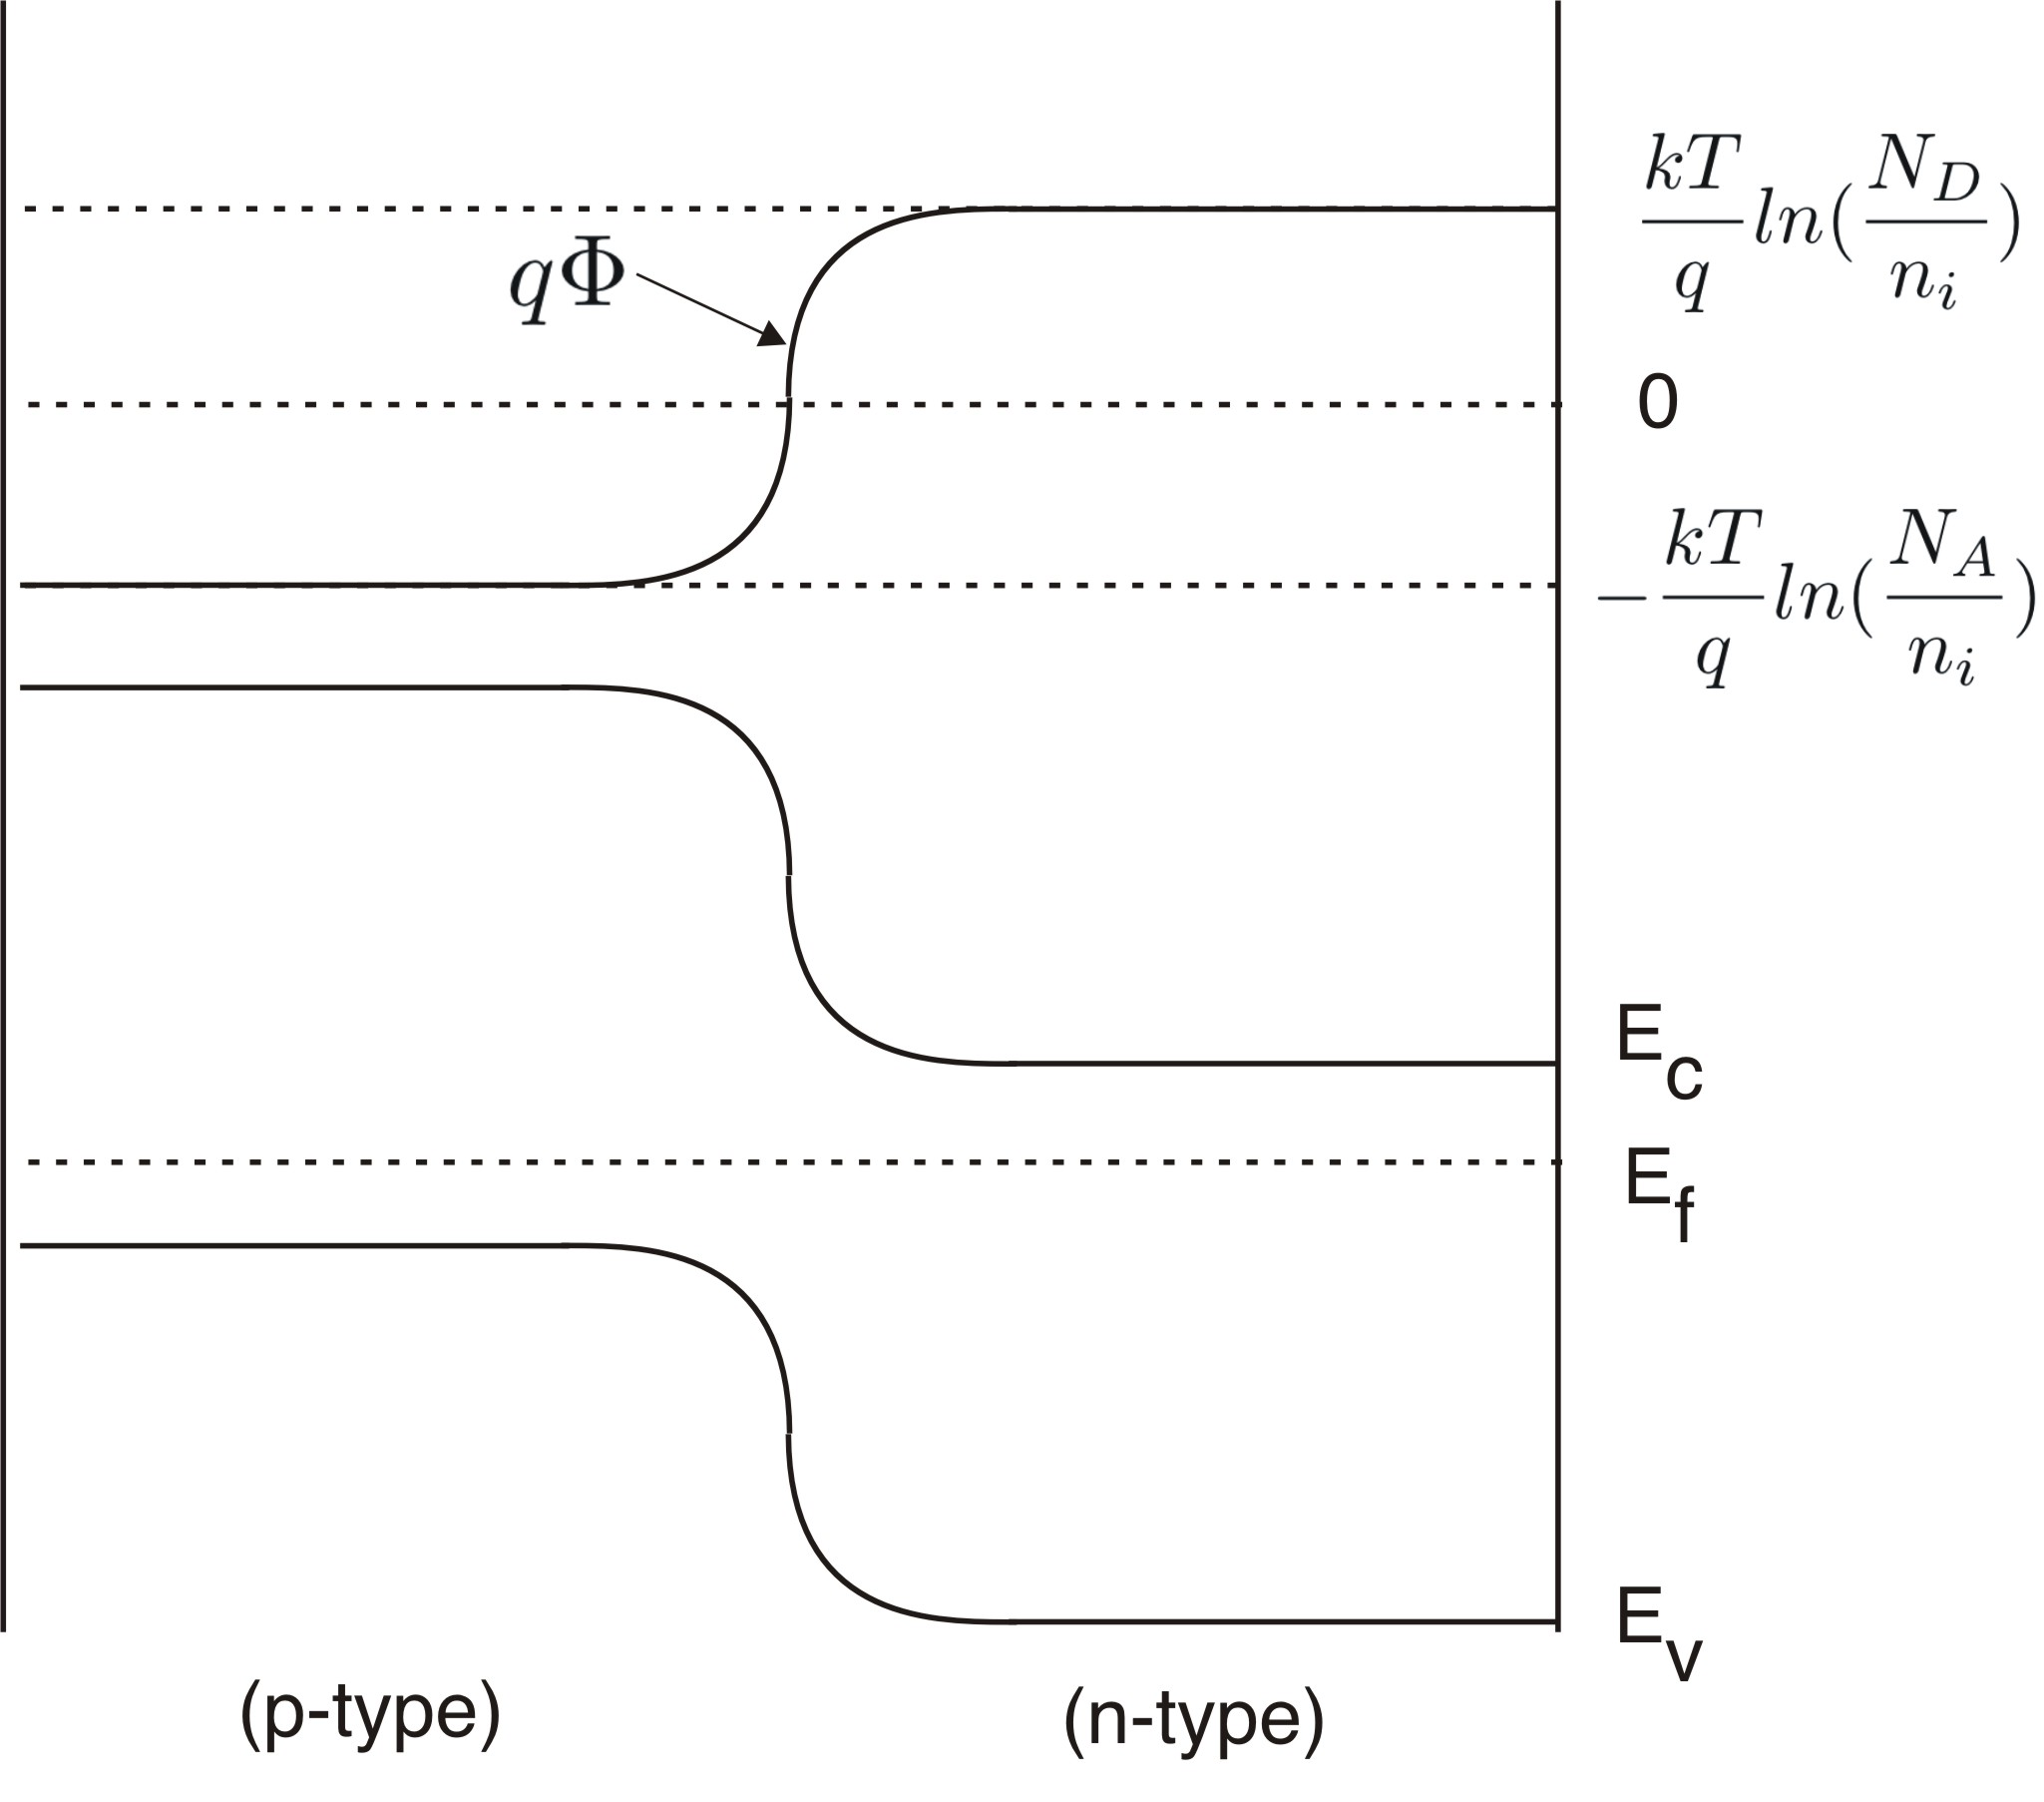
\includegraphics[width=4.050in,height= 3.600in]{neutral_contacts}}
  \caption[Neutral Contacts]{Neutral Contacts. \label{figNeutralContact}}
\end{figure}

$V_{bi}$ represents the extent of the energy band bending due to the doping
of a device.  While most of the dramatic changes will happen away from the
contact, near junctions, it is still incorporated into the voltage boundary
condition to maintain a flat potential near the contacts.  
Figure~\ref{figNeutralContact} shows the energy band variation across a PN
junction, and the corresponding electrostatic potential.  This variation is
due to the internal physics of the device, and needs to be there even in
the event of zero applied voltage.  This is partially enforced by the
solution to Poisson's equation, and also by the application of
equation~\ref{vbc_equ1}.

% Schottky contact figure, P-type

\subsubsection{Schottky Contacts}
In the case of a metal-semiconductor contact, it is necessary to add the
workfunction difference, $\Phi_{ms}$, to the potential in the
semiconductor~\cite{streetman}.  $\Phi_{m}$ is a constant for a given metal, and $\Phi_{s}$
is a function of the doping in the semiconductor.  The workfunction
potential, $\Phi$, when multiplied by q, is the difference between the
Fermi level and vacuum in the material.  In essence, the workfunction
difference represents the distance between the Fermi level in the metal and
the Fermi level in the semiconductor when considering the individual band
structures.

% Schottky contact figure, N-type
\begin{figure}[ht]
  \centering
  \scalebox{1.0}
  {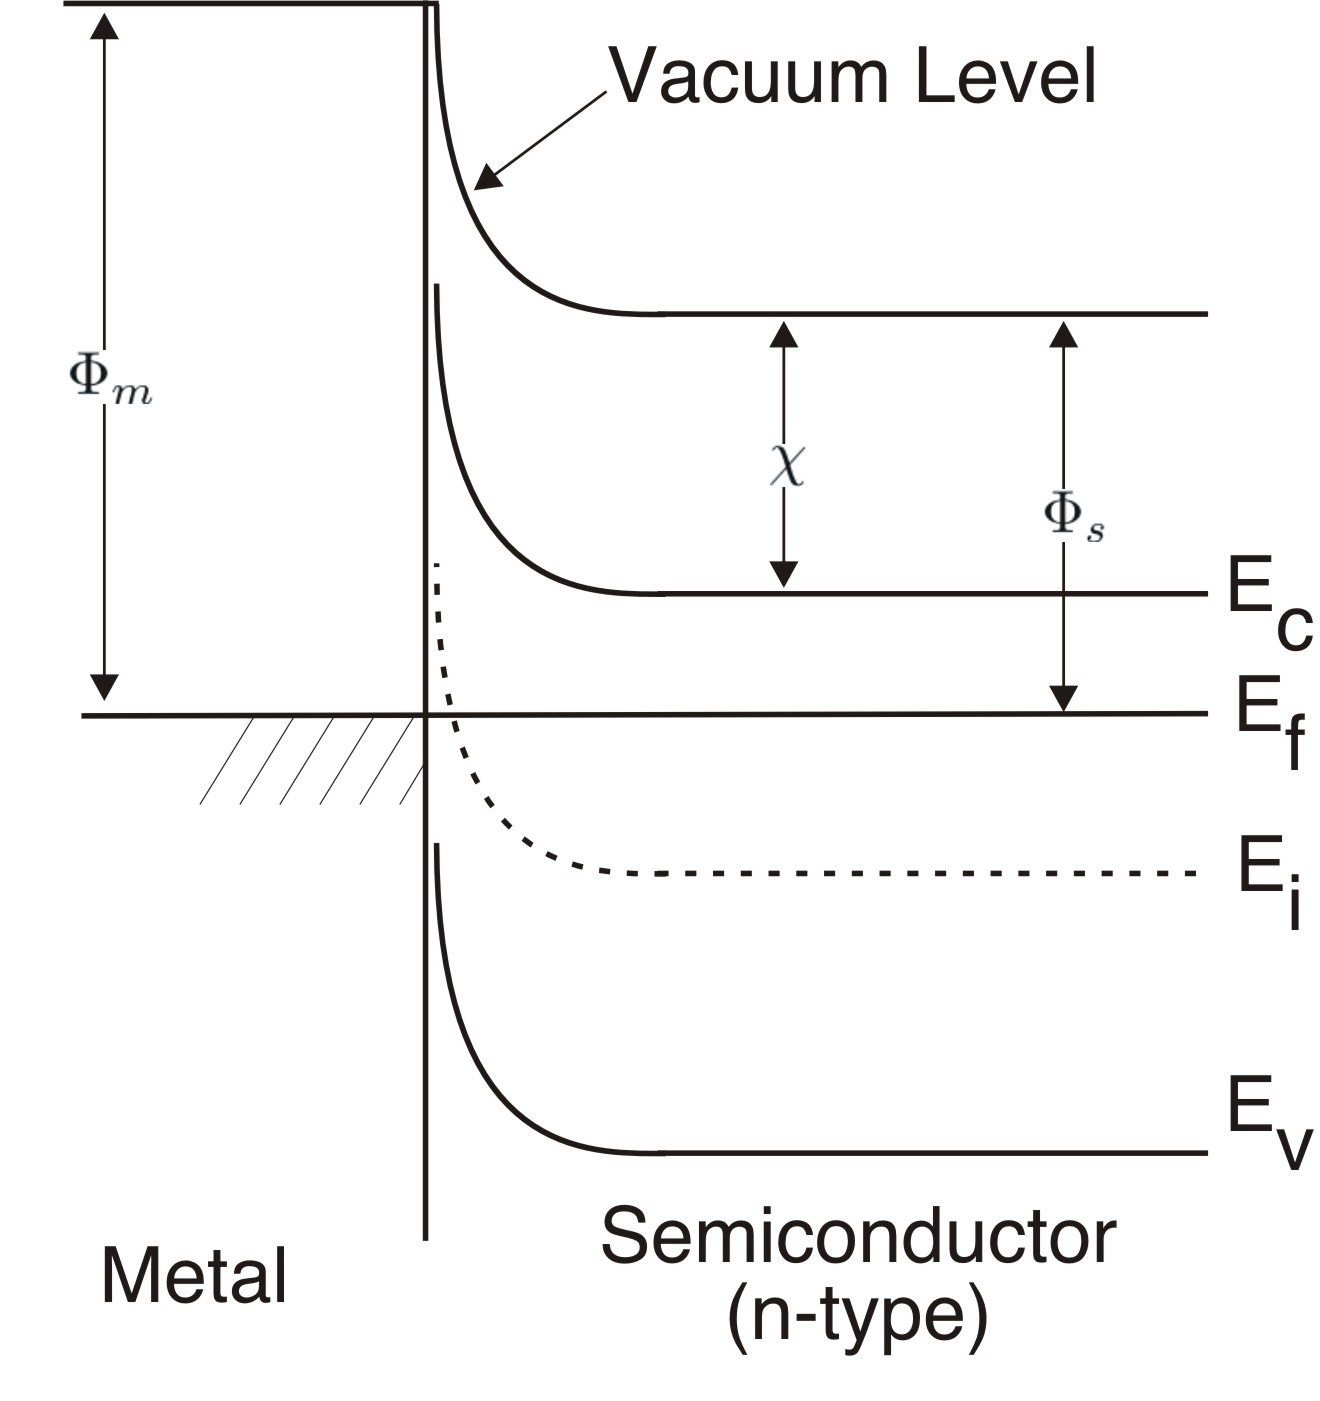
\includegraphics[width=3.300in,height= 3.500in]{schottky_bands}}
  \caption[Schottky Contact, N-type]{Schottky Contact, N-type. 
   \label{figSchottkyContactN}}
\end{figure}

% Schottky contact figure, P-type
\begin{figure}[ht]
  \centering
  \scalebox{1.0}
  {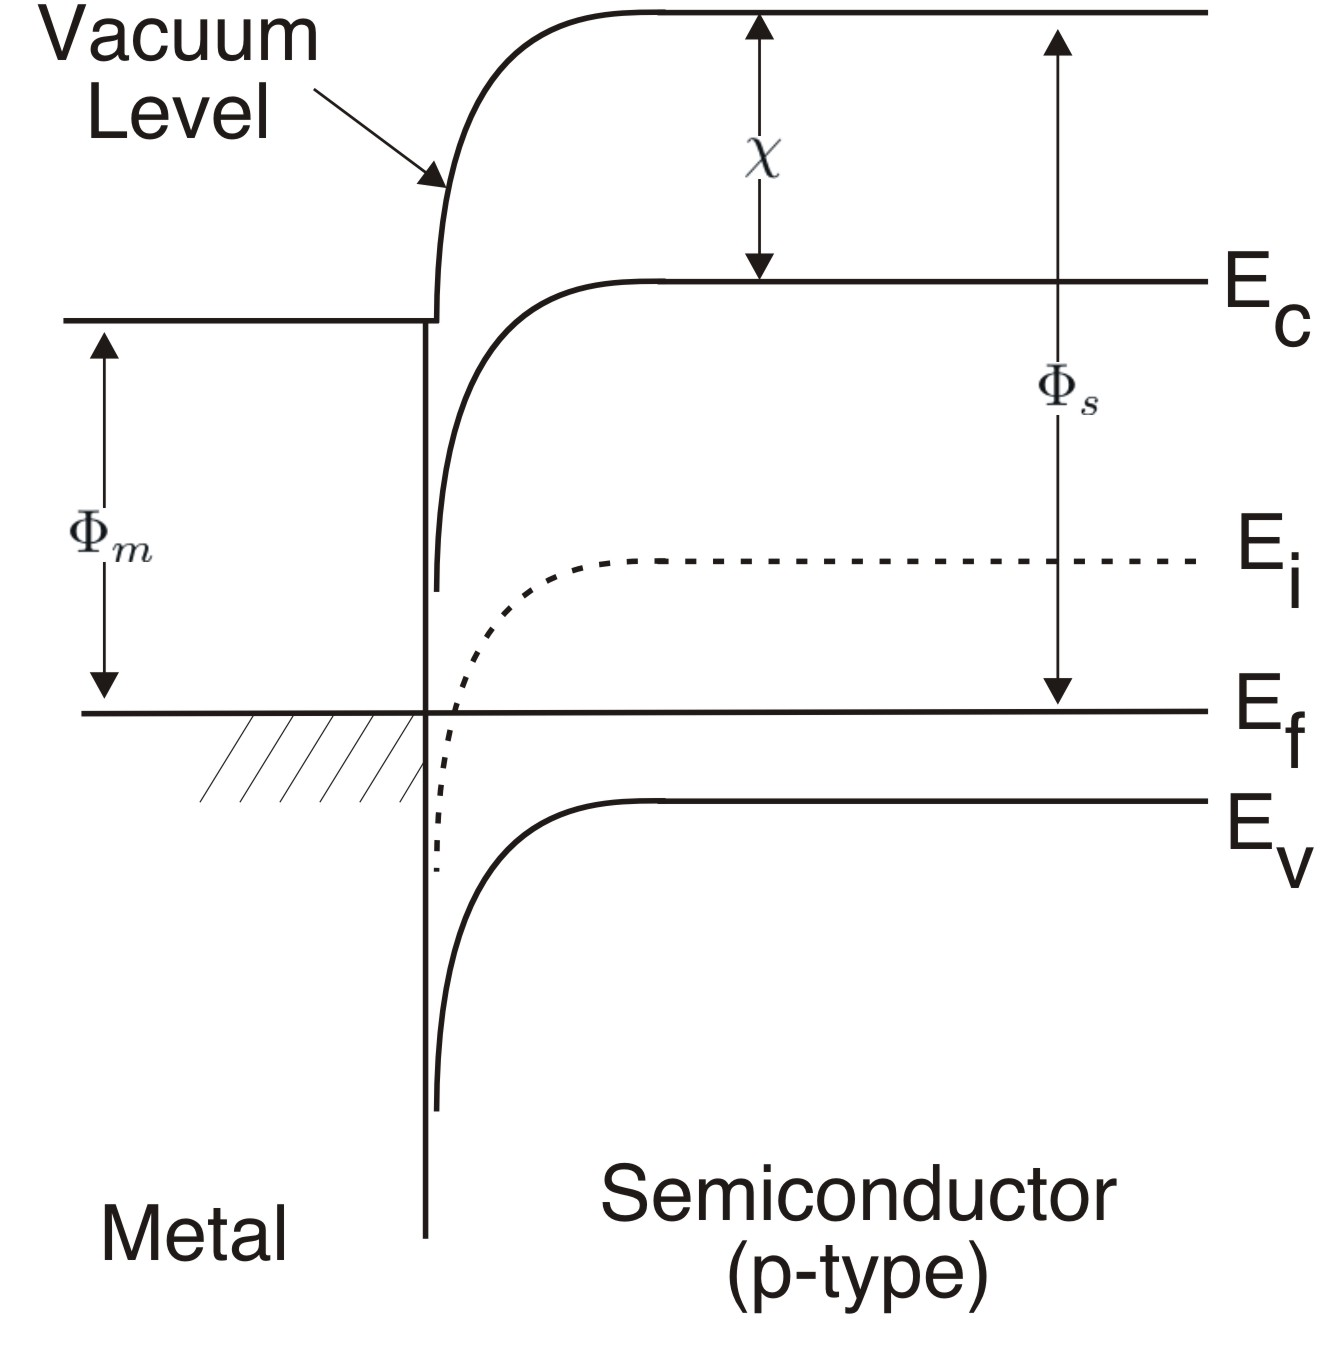
\includegraphics[width=3.300in,height= 3.400in]{schottky_bands_p}}
  \caption[Schottky Contact, P-type]{Schottky Contact, P-type. 
   \label{figSchottkyContactP}}
  
\end{figure}


In the case of an n-type semiconductor, the semiconductor workfunction can
be represented as

\begin{equation}
  \Phi_{s} = \chi + (E_{C}- E_{FS})/q
\end{equation}

where $\chi$ is the electron affinity in the semiconductor and q$\chi$ is the
distance between the conduction band and vacuum in the semiconductor.
$E_C$ is the conduction band energy and $E_{FS}$ is the Fermi level of the
semiconductor.  Rewriting this expression in terms of the doping 
concentration, it becomes

\begin{equation}
  \Phi_{s} = \chi + E_{g}/2 - V_{t}ln(\frac{N_{d}}{n_{i}})
\end{equation}

In the case of a p-type semiconductor, the semiconductor workfunction can
be represented as

\begin{equation}
  \Phi_{s} = \chi + E_{g}/2 + (E_{i}- E_{FS})/q
\end{equation}

where $E_{i}$ is the intrinsic value of the Fermi level, and can be
approximated as the halfway point between the conduction band ($E_{C}$) and the
valance band ($E_{V}$).
Rewriting this expression in terms of the doping concentration

\begin{equation}
  \Phi_{s} = \chi + E_{g}/2 + V_{t}ln(\frac{N_{a}}{n_{i}})
\end{equation}

For the TCAD devices in \Xyce{}, for a node at a metal-semiconductor
contact, the quantity $\Phi_{m} - \Phi_{s}$ is added to the potential at
the node to account for the metal-semiconductor barrier.  The current 
values of metal workfunctions used in \Xyce{} are given in
Table~\ref{workFuncTable}.  The values for electron affinity are given in
Table~\ref{elecAffinTable}.  
The boundary condition for a metal electrode in \Xyce{} is given by

\begin{equation}
 V_{bc} = V_{ckt} + V_{bi} + \Phi_{ms}
\end{equation}

where $V_{ckt}$ is the potential applied by the circuit to the electrode
and $V_{bi}$ is the "built-in" potential of the semiconductor, a
function of the semiconductor doping.

\newpage
\LTXtable{\textwidth}{workfuncTbl.tex}
\LTXtable{\textwidth}{elecAffinTbl.tex}
\newpage

\subsubsection{Metal-Oxide-Semiconductor Contacts}

To date in \Xyce{}, only semiconductor material is included in the PDE
solution domain.  Metals and oxide materials are only included
through boundary conditions.  This is an adequate approach for a lot of
problems.  For some problems (such as modeling of low-dose radiation
effects) modeling the oxide in more detail, as a PDE, will become necessary.
However, since oxides are usually very thin, compared with the
semiconductor domain, meshing both materials as part of the same simulation
is difficult.  Therefore, incorporating the effects of a gate oxide as part
of the gate boundary condition is a reasonable approach.

In the case of a contact to a metal-oxide-semiconductor structure, the
separation of the Fermi energies in the metal and the semiconductor at
equilibrium is due to two effects:  the workfunction difference between the
metal and the semiconductor, and the effective interface charge.  These two
effects cause the bands to bend at the surface in equilibrium.  The
flatband voltage is the sum of these two terms~\cite{streetman}:

\begin{equation}
  V_{FB} = \Phi_{ms} - \frac{Q_{i}}{C_{i}}
\end{equation}

where $\Phi_{ms}$ is the metal-semiconductor workfunction difference,
$Q_{i}$ is the value of interface charge (in $C/cm^{2}$), and $C_{i}$ is the
oxide capacitance per unit area, which is given by

\begin{equation}
  C_{i} = \frac{\epsilon_{ox} \epsilon_{0}}{x_{o}}
\end{equation}

The voltage $V_{FB}$ is the amount of bias which, when applied to the gate,
causes the electron energy bands to be flat.  This is the potential
that is added to a boundary node in \Xyce{} to account for a metal-oxide-semiconductor
barrier.  The overall boundary condition for a contact to a
metal-oxide-semiconductor structure is given by

\begin{equation}
  V_{bc} = V_{ckt} + V_{bi} + \Phi_{ms} - Q_{i}/C_{i}
\end{equation}

where $V_{ckt}$ is the potential applied by the circuit and $V_{bi}$ is the
"built-in" potential of the semiconductor.

\subsubsection{NMOS Device}

The default NMOS device used in \Xyce{} has a substrate doping
concentration of $1.0 \times 10^{16}/cm^{3}$ and an oxide thickness of $1.0
\times 10^{-6}cm$.  Since the ideal threshold voltage $V_{T}$ is given by

\begin{equation}
  V_{T} = 2 \phi_{F} + \frac{\epsilon_{s}}{\epsilon_{ox}} x_{o} 
\sqrt{\frac{2qN_{A}\phi_{F}}{\epsilon_{s}\epsilon_{0}}}
\end{equation}

$V_{T}$ is equal to 0.892 V. for this device.  Note that 
\begin{equation}
  \phi_{F} = \frac{1}{q}[E_{i}(bulk) - E_{F}] = \frac{kT}{q}
  ln(\frac{N_{A}}{n_{i}})
\end{equation}

for a p-type semiconductor substrate and

\begin{equation}
 \phi_{F} = - \frac{kT}{q} ln(\frac{N_{D}}{n_{i}})
\end{equation}

for an n-type substrate.
%%

%%% Local Variables:
%%% mode: latex
%%% End:

% END of Xyce_RG_PDE.tex ************


\cleardoublepage
% Sandia National Laboratories is a multimission laboratory managed and
% operated by National Technology & Engineering Solutions of Sandia, LLC, a
% wholly owned subsidiary of Honeywell International Inc., for the U.S.
% Department of Energy’s National Nuclear Security Administration under
% contract DE-NA0003525.

% Copyright 2002-2021 National Technology & Engineering Solutions of Sandia,
% LLC (NTESS).


%%-------------------------------------------------------------------------
%% Purpose        : Second Section LaTeX Xyce Reference Guide
%% Special Notes  : Graphic files (pdf format) work with pdflatex.  To use
%%                  LaTeX, we need to use postcript versions.  Not sure why.
%% Creator        : Scott A. Hutchinson, Computational Sciences, SNL
%% Creation Date  : {05/23/2002}
%%
%%-------------------------------------------------------------------------

\chapter{Command Line Arguments}
\label{cmd_line_args}
\index{command line!arguments}

\Xyce{} supports a handful of command line arguments which must be given {\em
  before} the netlist filename.  While most of these are intended for general
use, others simply give access to new features that, while supported, are not 
enabled by default.  The general usage is as follows:
\begin{vquote}
  Xyce [arguments] <netlist filename>
\end{vquote}

Table~\ref{cmd_line_arg_list} gives a list of supported command line
options.\footnote{Note that the ``-h'' option might list command line options not present 
in this table.  These extra options are generally deprecated and should not be used.  Only 
the options listed in the table are considered supported features.}

% Sandia National Laboratories is a multimission laboratory managed and
% operated by National Technology & Engineering Solutions of Sandia, LLC, a
% wholly owned subsidiary of Honeywell International Inc., for the U.S.
% Department of Energy’s National Nuclear Security Administration under
% contract DE-NA0003525.

% Copyright 2002-2020 National Technology & Engineering Solutions of Sandia,
% LLC (NTESS).

%%
%% Command line arguments table.
%%
\small
\begin{longtable}[htbp]
{|>{\setlength{\hsize}{0.5\hsize}}Y|
>{\setlength{\hsize}{1.0\hsize}}Y|
>{\setlength{\hsize}{0.75\hsize}}Y|
>{\setlength{\hsize}{0.55\hsize}}Y|} 

\caption [List of \Xyce{} command line arguments.]{List of \Xyce{} command line arguments. \label{cmd_line_arg_list}} \index{command line} \\
\hline

\rowcolor{XyceDarkBlue}{\color{white}\bf Argument} &
{\color{white}\bf Description} &
{\color{white}\bf Usage} &
{\color{white}\bf Default} \endhead \hline

-h &
Help option. Prints usage and exits. &
\verb+-h+ &
- \\ \hline

-v &
Prints the version banner and exits. &
\verb+-v+ &
- \\ \hline


-delim &
Set the output file field delimiter. &
%% have to break line to keep table neat
\verb+-delim+
\verb+<TAB|COMMA|string>+ &
- \\ \hline

-o &
Place the results into specified file. &
\verb+-o  <file>+ &
- \\ \hline

-l &
Place the log output into specified file. &
\verb+-l  <file>+ &
- \\ \hline

-r &
Output a binary rawfile. &
\verb+-r  <file>+ &
- \\ \hline

-a &
Use with \verb+-r+ to output a readable (ASCII) rawfile. &
\verb+-r  <file> -a+ &
- \\ \hline

-nox &
Use the NOX nonlinear solver. &
\verb+-nox  <ON|OFF>+ &
on \\ \hline

-linsolv &
Set the linear solver. &
%% have to break line to keep table neat
\verb+-linsolv+
\verb+<KLU|+
\verb+KSPARSE|SUPERLU|+
\verb+AZTECOO|BELOS>+ &
klu(serial) and aztecoo(parallel) \\ \hline

-param &
Print a terse summary of model parameters, device parameters and default values. &
\verb+-param+ &
- \\ \hline

-syntax &
Check netlist syntax and exit.&
\verb+-syntax+ &
- \\ \hline

-norun &
Check netlist syntax and topology and exit. &
\verb+-norun+ &
- \\ \hline

-quiet &
Suppress some of the simulation-progress messages
sent to stdout for transient simulations. &
\verb+-quiet+ &
- \\ \hline

-namesfile &
Output a list of all solution variables generated by the netlist
into \tt{<filename>} &
%% have to break line to keep table neat
\verb+-namesfile+
\verb+<filename>+ &
- \\ \hline

-randseed &
Set random number seed for expression library's random number functions
 and also \texttt{.SAMPLING} analysis. &
\verb+-randseed <number>+ &
If not provided, Xyce will select a seed using the system ``time'' function.  \\ \hline

-maxord &
Maximum time integration order. &
\verb+-maxord <1..5>+ &
- \\ \hline

-jacobian\_test &
Jacobian matrix diagnostic. &
\verb+-jacobian_test+ &
- \\ \hline
\end{longtable}



A few other command line options are available that are typically only used in Xyce development.  
For example the options {\tt -param}, {\tt -info}, {\tt -doc} and {\tt -doc\_cat} are 
used to generate the device tables in this guide.  The options {\tt -jacobian\_test} 
and {\tt -namesfile} can be useful in debugging new devices in \Xyce{}.  The option
 {\tt -namesfile} is also useful for determining the ``fully qualified node
names'', including the subcircuit hierarchy, for nodes and internal variables for mutual
inductors.  The {\tt .PRINT} section \ref{.PRINT} has more information on, and examples for,
the {\tt -namesfile} command line option.

\section{Hspice extensions}
\label{hspice_ext_cmd_line}

The command line argument \verb+-hspice-ext+ is more complicated than most, so its explanation is given in this section.
The second argument to \verb+-hspice-ext+ can either be a single string or can be a comma separated list.
\begin{itemize}
\item Using \verb+all+ will enable all the features.   
\item Using \verb+units+ sets the use of the ``atto'' prefix, designated by ``a'', to mean a mutliplier of ``1E-18''.   Without this setting, the ``a'' prefix means units of amperes.
\item Using \verb+math+ sets the use of Hspice style math operators.  Most importantly, it forces ``log'' to mean the natural logarithm, rather than the base 10 logarithm.
\item Using \verb+separator+ sets the use of the period ``.'' for subcircuit name separation.  If this is not set, the colon ``:'' is used instead.
\end{itemize}

\chapter{Runtime Environment}
\label{runtime}

\section{Running Xyce in Serial}

After ensuring that the directory into which \Xyce{} was installed is
in your PATH variable, one merely executes the code by running the
command, \texttt{Xyce} with the desired netlist name appended.

\section{Running Xyce in Parallel}

Open MPI must be installed on the host machine.  It may be download from 

\texttt{http://www.open-mpi.org/}.  Consult the documentation for help with installation.

After ensuring that the both the directory into which \Xyce{} was
installed and the directory in which mpirun is found are in your PATH
variable, one merely executes the code by running the command,
\texttt{mpirun [mpirun options] Xyce [xyce options]} with the desired
netlist name appended.

\section{Running Xyce on Sandia HPC and CEE Platforms}



This version of \Xyce{} has been installed centrally on Sandia HPC
and CEE platforms, and requires metagroup access.  Contact the \Xyce{} team
for details on how to obtain this access.

Once you have registered for metagroup membership, the central
installs of \Xyce{} may be accessed by a module load.

\verb+module load Xyce+ adds all required modules and sets all
required environment variables to access the normal version of
\Xyce{}.  \verb+module load XyceRad+ does the same thing for the
version \Xyce{} containing Sandia proprietary models.

\verb+module help Xyce+ provides some additional information about
what the module does.

Consult the system documentation for help with submitting jobs on
these platforms.

\verb+https://computing.sandia.gov/+

\chapter{Setting Convergence Parameters for Xyce}
\label{Conv_Guidelines}
\index{convergence}\index{\Xyce{}!convergence}\index{parameters!convergence}

Because the solution algorithms and methods within \Xyce{} are different than
those used by other circuit simulation tools (e.g., SPICE), the overall
convergence behavior is sometimes different, as are the parameters which control
this behavior.

\section{Adjusting Transient Analysis Error Tolerances}
\index{transient analysis!error tolerances}\index{solvers!time
  integration!options}

\Xyce{} uses a variable order trapezoid integration as its default
scheme, and this method may also be requested explicitly with the
\textrmb{TIMEINT} option \texttt{METHOD=trap} or
\texttt{METHOD=7}. Trapezoid time-stepping is second order accurate
and does not have any numerical dissipation in its local truncation
error. Variable order trapezoid integration dynamically uses Backward
Euler (BE) and trapezoid rule. When \texttt{ERROPTION=1} is set with
\texttt{METHOD=7}, trapezoid rule is used almost exclusively (BE
only used at breakpoints). See table~\ref{TimeIntPKG} for details.

Another time integration option is the second-order Gear method.  It
may be selected with the \textrmb{TIMEINT} option \texttt{METHOD=gear} or
\texttt{METHOD=8}. See table~\ref{TimeIntPKG} for details.

\subsection{Setting \textrmb{RELTOL} and \textrmb{ABSTOL}}
\index{\Xyce{}!\texttt{RELTOL}}\index{\Xyce{}!\texttt{ABSTOL}}
In \Xyce{}, both the time integration package and the nonlinear solver package
have \textrmb{RELTOL} and \textrmb{ABSTOL} settings.  Some general guidelines for
settings parameters are~\cite{Petzold:1996}:
\begin{XyceItemize}
\item Use the \emph{same} \textrmb{RELTOL} and \textrmb{ABSTOL} values for both
  the \textrmb{TIMEINT} and the \\ \textrmb{NONLIN-TRAN} \textrmb{.OPTIONS}
  statements.
\item For a conservative approach (i.e., safe), set \texttt{RELTOL=1.0E-(\emph{m}+1)}
  where \texttt{\emph{m}} is the desired number of significant digits of
  accuracy.
\item Set \textrmb{ABSTOL} to the smallest value at which the solution
  components (either voltage or current) are essentially insignificant.
\item Note that the above suggests that $\textrmb{ABSTOL}<\textrmb{RELTOL}$.
\end{XyceItemize}

The current defaults for these parameters are \texttt{ABSTOL=1.0E-6} and
\texttt{RELTOL = 1.0E-3}.  For a complete list of the time integration
parameters, see chapter ~\ref{Netlist_Commands}.

\section{Adjusting Nonlinear Solver Parameters (in transient mode)}
\index{solvers!nonlinear!options}

In \Xyce{}, the nonlinear solver options for transient analysis are set using
the \texttt{.OPTIONS NONLIN-TRAN} line in a netlist.  This subsection gives
some guidelines for setting this parameters.
\begin{XyceItemize}
\item For guidelines on setting \textrmb{RELTOL} and \textrmb{ABSTOL}, see above.
\item \textrmb{RHSTOL} -- This is the maximum residual error for each nonlinear
  solution.  \Xyce{} uses this as a ``safety'' check on nonlinear
  convergence.  Typically, \texttt{1.0E-2} (the default) works well.
\item \textrmb{DELTAXTOL} -- This is the weighted update norm tolerance and is
  the primary check for nonlinear convergence.  Since it is weighted (i.e.,
  normalized using \textrmb{RELTOL} and \mbox{\textrmb{ABSTOL}}), a value of
  \texttt{1.0} would give it the same accuracy as the time integrator.  For
  robustness, the default is \texttt{0.33} but sometimes a value of
  \texttt{0.1} may help prevent ``time-step too small'' errors.  A value of
  \texttt{0.01} is considered quite small.
\item \textrmb{MAXSTEP} -- This is the maximum number of Newton (nonlinear)
  steps for each nonlinear solve.  In transient analysis, the default is
  \texttt{20} but can be increased to help prevent ``time-step too small''
  errors.  This is roughly equivalent to \textrmb{ITL4} in SPICE.
\end{XyceItemize}

\chapter{Quick Reference for Users of Other SPICE 
Circuit Simulators}
\label{PSpice_Ref}
\index{PSpice}
\index{Users of PSpice}

This chapter describes many of the differences between \Xyce{} and
other SPICE-like circuit simulaters.  The primary focus is on the difference
between Orcad PSpice and \Xyce{}, with an eye towards providing the ability for those
familiar with using PSpice to begin using \Xyce{} quickly.   PSpice compatibility 
was an early focus for the Xyce project.

The Xyce team also supports a netlist translation tool, XDM (for Xyce Data 
Model)~\cite{XDMv2.3}.  This tool supports translation of netlists in Pspice, 
Hspice and Spectre format into Xyce formatted netlist files.  There is also a 
\Xyce{} command line option (\texttt{--hspice-ext all}) which is designed to 
assist with a handful of Hspice syntax issues that are particularly 
difficult to translate.

This chapter is likely not complete, and \Xyce{} users might also consult
specific sections of this Reference Guide about particular \Xyce{} commands.
Those sections may have additional information on Xyce's incompatibilities with
other circuit simulators, and how to work around them.  
\section{Differences Between Xyce and PSpice}
This section is focused on the differences between \Xyce{} and PSpice.
However, some of this discussion also applies to other SPICE-like
circuit simulators. 

\subsection{Command Line Options}
Command line arguments are supported in \Xyce{} but they are different than
those of PSpice.   For a complete reference, see Chapter~\ref{cmd_line_args}. 

\subsection{Device Support}
Most, but not all, devices commonly found in other
circuit simulation tools are supported.  \Xyce{} also contains enhanced versions of
many semiconductor devices that simulate various environmental effects.  For the
complete list, please see the
Analog Device Summary in Table~\ref{Device_Summary}.

\subsection{ .OPTIONS Support}
For the specific devices or models that are supported in \Xyce{}, most of the
standard netlist inputs are the same as those in standard SPICE.
However, the \textrmb{.OPTIONS} command has several additional features used to
expose capabilities specific to \Xyce{}.  In particular, \Xyce{} does not
support the standard PSpice format \textrmb{.OPTIONS} line in netlists.
Instead, options for each supported package are called according to the
following format.

\begin{Command}
\format
.OPTIONS <pkg> [<tag>=<value>]*

\arguments

\begin{Arguments}
\argument{DEVICE}       Device Model
\argument{TIMEINT}      Time Integration
\argument{NONLIN}       Nonlinear Solver
\argument{NONLIN-TRAN}  Transient Nonlinear Solver
\argument{NONLIN-HB}    HB Nonlinear Solver
\argument{LOCA}         Continuation/Bifurcation Tracking
\argument{LINSOL}       Linear Solver
\argument{LINSOL-HB}    HB Linear Solver
\argument{OUTPUT}       Output
\argument{RESTART}      Restart
% \argument{MPDEINT}      MPDE
\argument{HBINT}        Harmonic Balance (HB)
\argument{SENSITIVITY}  Direct and Adjoint sensitivity analysis
\end{Arguments}

\end{Command}

\index{\texttt{.OPTIONS}}

For a complete description of the supported options in \Xyce{}, see
section~\ref{Options_Reference}.  

Known caveats are that the \texttt{ABSTOL} options have different definitions 
in PSpice and \Xyce{}.  Also, a PSpice \texttt{.OPTIONS VNTOL=<value>} line can 
be mapped into these two \Xyce{} lines:
\begin{vquote}
.OPTIONS NONLIN ABSTOL=<value> 
.OPTIONS NONLIN_TRAN ABSTOL=<value>
\end{vquote}

The PSpice \texttt{ITL1} and \texttt{ITL4} options are similar to the \Xyce{} \texttt{MAXSTEPS}.
In PSpice, \texttt{ITL1} affects \texttt{.DC} analyses, while \texttt{ITL4} 
affects \texttt{.TRAN} analyses.  In \Xyce{}, \texttt{.OPTIONS NONLIN}
refers to options for \texttt{.DC} analyses, while \texttt{.OPTIONS NONLIN-TRAN}
refers to options for \texttt{.TRAN} analyses.  So, a feasible mapping is 
PSpice \texttt{.OPTIONS ITL1=20} becomes \texttt{.OPTIONS NONLIN MAXSTEP=20}
in \Xyce{}.  Similarly, PSpice \texttt{.OPTIONS ITL4=20} becomes 
\texttt{.OPTIONS NONLIN-TRAN MAXSTEP=20} in \Xyce{}.  However, given that
PSpice and Xyce{} use different default values for \texttt{ITL1} and \texttt{ITL4} 
vs. \texttt{MAXSTEPS}, the best approach may be to not translate the \texttt{ITL1} and 
\texttt{ITL4} lines into the corresponding \Xyce{} netlist.

\subsection{.PROBE vs. .PRINT}
\Xyce{} does not support the ``\textrmb{.PROBE}'' statement.  Output of Probe-format
files, in .csd format, that are readable by PSpice is done using the \textrmb{.PRINT} netlist statement.
See section~\ref{.PRINT} for the syntax for \texttt{FORMAT=PROBE}.  That section
also describes wildcard support and access to subcircuit nodes in \Xyce{}, both of
which are different than PSpice.

\Xyce{} does not support PSpice style abbreviations in the \textrmb{.PRINT}
statement.  For example, to print out the value of the voltage at node
\texttt{A} in a transient simulation you must request \mbox{\texttt{.PRINT TRAN V(A)}},
not \mbox{\texttt{.PRINT TRAN A}}.  \Xyce{} also does not support \texttt{N()} as a
synonym for \texttt{V()} on \texttt{.PRINT} lines.

\subsection{Converting PSpice ABM Models for Use in Xyce}
\label{Converting_ABM}
\index{device!ABM device!PSpice equivalent}

\Xyce{} is almost fully compatible with PSpice with respect to analog
behavioral models.  This includes the
\texttt{E}\index{PSpice!\texttt{E} device},
\texttt{F}\index{PSpice!\texttt{F} device},
\texttt{G}\index{PSpice!\texttt{G} device}, and
\texttt{H}\index{PSpice!\texttt{H} device} 
device types.  A notable exception to this compatibility is in the use of lead and device
currents in expressions used in controlled source definitions.  That feature is not 
supported in \Xyce{}.  In addition, the \texttt{FREQ},\texttt{LAPLACE} and 
\texttt{CHEBYSHEV} forms for E and G sources or the \texttt{ERROR} qualifier are 
not supported in \Xyce{}..
  
\subsection{Usage of \textrmb{.STEP} Analysis}

The implementation of \textrmb{.STEP} in \Xyce{} is not the
same as that of PSpice.  See section~\ref{.STEP} for the syntax and
function of the \textrmb{.STEP} function in \Xyce{}.

\subsubsection{Model Parameter Sweeps}

PSpice requires extra keywords to apply a \textrmb{.STEP} statement to a
model parameter.  \Xyce{} handles model parameters differently, and is
actually somewhat more flexible than PSpice.  Unfortunately, this means
that the two specifications are not compatible.

A model parameter in PSpice would be handled like this:
\begin{vquote}
R1 1 2 RMOD 1
.model RMOD RES(R=30)
.step RES RMOD(R) 30 50 5
\end{vquote}
The equivalent way to specify this in \Xyce{} would be:
\begin{vquote}
R1 1 2 RMOD 1
.model RMOD RES(R=30)
.step RMOD:R 30 50 5
\end{vquote}
Note that \Xyce{} does not require the \texttt{RES} keyword on the
\texttt{.STEP} line.  In PSpice, this keyword is needed to specify 
what type of model is being used.  \Xyce{} actually has more flexibility
than PSpice in this regard---any model or instance variable can be set on
the \texttt{.STEP} line using the same syntax.

\Example{\texttt{.step D101:IS 1.0e-3 5.0e-3 1.0e-3}}

In this example, \texttt{D101} is the name of a model or instance, 
and \texttt{IS} is the name of the parameter within that model or instance.

\subsection{Behavioral Digital Devices}
There are at least four significant differences.  First, the instance line
syntax for the \Xyce{} digital behavioral devices differs from PSpice.
Second,  \Xyce{} uses one model card for the timing and Input/Output (I/O)
characteristics, while PSpice uses separate model cards for timing and I/O
characteristics.  The model cards also have different parameters. 
Third, \Xyce{} does support the \texttt{DIGINITSTATE} option. However, it has a
different default value than in PSpice.  So, the DCOP calculations for flip-flops and latches may
be different in some cases between \Xyce{} and PSpice.  Finally, closely spaced input
transitions to a gate (e.g., ones spaced by less than the \texttt{DELAY}
parameter of the \Xyce{} model) may produce different behaviors in \Xyce{}
and PSpice.  Please consult Section \ref{U_DEVICE} for more details.

\subsection{Power Dissipation}
PSpice supports printing the power dissipation of a device via syntax like
\texttt{W(<name>)}.  At this time, not all \Xyce{} devices support power calculations. 
In addition, the \Xyce{} results for the FET semiconductor devices (J, M and Z devices) may 
differ from the PSpice results.  Consult the Features Supported by Xyce Device Models table
in Section \ref{Analog_Devices} and the individual sections on each device for more details.  
Additional limitations on lead current and power
calculations in \Xyce{} are given in Section \ref{leadCurrentPowerCalculations}.

Example work-arounds are as follows, using either the
node voltage at Node 2 or the lead current through Resistor 2:

\begin{vquote}
.DC V1 0 5 1
.param R2VAL=10
V1 1 0 5V
R1 1 2 10
R2 2 0 \{R2VAL\}
.PRINT DC V(2) \{V(2)*V(2)/R2VAL\} \{I(R2)*I(R2)*R2VAL\}
\end{vquote}

\subsection{Dependent Sources with TABLE Syntax}
\label{DS_TABLE_SYNTAX_DIFF}
The documented PSpice syntax for the \texttt{TABLE} form of the E and G sources
is identical to the \Xyce{} syntax for those two devices.  As an example, consider 
this E-source netlist line which conforms to the documented PSpice and Xyce 
syntaxes:
\begin{vquote}
E5  5 0 TABLE {V(1,0)} = (-2,-3) (2,3)
\end{vquote}
There is an equal sign between the expression \texttt{\{V(1,0)\}} and the list of
value pairs (e.g., before \texttt{(-2,-3)}).  There is also a comma between the two values
in each set of value pairs.  However, it has been observed that some PSpice versions 
will accept variants of the documented PSpice syntax.  As examples, PSpice might 
use this \texttt{TABLE} syntax, where the equal sign between the expression and the 
list of value pairs is missing and there is an extra set of parentheses around 
the list of value pairs:
\begin{vquote}
TABLE \{EXPR\} ((x1,y1) (x2,y2) \ldots (xn, yn))
\end{vquote}
PSpice might also specify the \texttt{TABLE} syntax without the commas between the 
two values in each set of value-pairs. For example, this is a legal syntax in some 
PSpice versions:
\begin{vquote}
TABLE \{EXPR\} = (x1 y1) (x2 y2) \ldots (xn yn)
\end{vquote}
So, the generic solution is to change these alternative PSpice syntaxes (and possibly 
others) to conform with the \Xyce{} E and G source \texttt{TABLE} syntax, which is
(see also Sections \ref{E_DEVICE} and \ref{G_DEVICE}):
\begin{vquote}
TABLE \{EXPR\} = (x1,y1) (x2,y2) \ldots (xn, yn)
\end{vquote}

\subsection{MODEL STATEMENTS}
\label{MODEL_STATEMENT_SYNTAX_DIFF}
In PSpice, some \texttt{.MODEL} statements may have commas separating the list
of parameters, which causes problems in \Xyce{}.  A simple workaround is to
replace those commas with spaces in the corresponding \Xyce{} \texttt{.MODEL}
statements.

In PSpice, some \texttt{.MODEL} statements may not have parentheses
surrounding the list of parameters.  While Xyce also does not require parentheses
in model cards, parentheses are accepted.  The only \Xyce{} requirement is that if
they are used then they must be paired with one left parenthesis before all of the
parameters and one right parentheses after all of the parameters. It is an error
to have unmatched parentheses.  

PSpice syntaxes where only a subset of the model 
parameters are enclosed within parentheses are also not supported in \Xyce{}. 
A PSpice example is:
\begin{vquote}
.model somebjt NPN Is=1e-16 (Xti=3 Bf=100) Eg=1.11 NC=2
\end{vquote}

Nested parentheses, as is often seen when a \texttt{DEV} (deviation) is specified 
for a parameter in a PSpice model statement, are also not allowed in \Xyce{}.  A PSpice
example is:
\begin{vquote}
.model someotherbjt NPN(Is=1e-16 Xti=3 (Bf=100 DEV=5\%) Eg=1.11 NC=2)
\end{vquote}

The previous PSpice example also raises the issue of model parameters that are supported
in PSpice but not in \Xyce{}.  It that case, \Xyce{} will issue a warning about the
invalid parameter and the simulation will run.

Another common issue is a PSpice model parameter (e.g., \texttt{BV=}) without a value.  
That PSpice syntax error is often silently ignored in PSpice, but flagged as a parsing 
error in a \Xyce{} netlist.  

Temperature coefficient (\texttt{TC}) specifications can be a problem also.  The 
documented PSpice syntax is this, with a comma between the two values.  

\begin{vquote}
TC=0.1,0.1
\end{vquote}

However, it has been observed that some PSpice versions allow the TC parameter to 
omit the comma between those two values.  That is not legal in \Xyce{}.

\subsection{.NODESET and .IC Statements}
\Xyce{} and PSpice differ in their capabilities to handle \texttt{.NODESET} and 
\texttt{.IC} statements in subcircuits.  See sections ~\ref{NODESET_section} 
and ~\ref{IC_section} for more details.

\subsection{Piecewise Linear Sources}
\label{PWL_SOURCE_SYNTAX_DIFF}
The preferred \Xyce{} syntax for PWL sources does not use parentheses or commas within
the time-voltage pair listing.  See Section \ref{I_DEVICE} for more details.

The \Xyce{} PWL source does not support the PSpice \texttt{.IN} format for file input.  
See Section \ref{I_DEVICE} for the ASCII text and \texttt{.csv} formats supported 
by \Xyce{} for file input.

The \Xyce{} repeat \texttt{R=<value>} syntax for PWL sources is not compatible with 
the PSpice \texttt{REPEAT} syntax for PWL sources.  Some work-arounds are as follows.
This PSpice \texttt{REPEAT FOREVER} syntax:
\begin{vquote}
VPWL1 1 0 PWL REPEAT FOREVER (0,0) (0.5,1) (1,0)
+ ENDREPEAT
\end{vquote}
is equivalent to this \Xyce{} syntax:
\begin{vquote}
VPWL1 1 0 PWL 0 0 0.5 1 1 0 R=0
\end{vquote}
Similarly, if the PSpice source has its time-voltage pairs in a \texttt{.csv}
file, and the specified waveform starts at time=0, then this PSpice syntax:
\begin{vquote}
VPWL2 2 0 PWL 
+ REPEAT FOREVER
+ FILE "data.csv"
+ ENDREPEAT
\end{vquote}
is equivalent to this \Xyce{} syntax:
\begin{vquote}
VPWL2 2 0 PWL file "data.csv" R=0
\end{vquote}
For more general PSpice \texttt{REPEAT} syntaxes, and especially for the PSpice
\texttt{REPEAT for N} syntax, the user might have to manually duplicate the 
PSpice waveform in a \texttt{.csv} file.

\subsection{.AC Output}
The \Xyce{} .csd file format for a \texttt{.AC} analysis is different than the
PSpice format, but is still viewable in the PSpice A/D waveform viewer.  This
PSpice \texttt{.PROBE} statement:
\begin{vquote}
.PROBE/CSDF V([1b]) VR([1b]) VI([1b])
\end{vquote}
will produce \#N and \#C lines in its netlistName.csd file like this, where the
real and imaginary parts of V(1b) are output for each data point on the \#C line.
The end-user can then use the PSpice A/D UI to choose to plot the VR and VI
quantities.
\begin{vquote}
#N
`V(1b)' `V(1b)' `V(1b)'
#C 1.0000000000E01 3
2.470E-02/-1.552E-01:1 2.470E-02/-1.552E-01:2 2.470E-02/-1.552E-01:3
\end{vquote}

This corresponding \Xyce{} .PRINT AC statement:
\begin{vquote}
.PRINT AC FORMAT=PROBE V(1b) VR(1b) VI(1b)
\end{vquote}
will produce \#N and \#C lines in its netlistName.csd file like this, where the real
and imaginary parts of V(1b) are still output on the \#C line.  However, in \Xyce{},
the VR() and VI() operators return real-valued quantities as shown below.  This
\Xyce{} formatted file is still viewable in PSpice A/D.
\begin{vquote}
#N
`V(1b)' `VR(1b)' `VI(1b)'
#C 1.0000000000E01 3
2.470e-02/-1.552e-01:1 2.470e-02/0.000e+00:2 -1.552e-01/0.000e+00:3
\end{vquote}

\subsection{Additional differences}
Some other differences between \Xyce{} and PSpice are described in 
Table~\ref{Incompat_PS}.  Users should also consult 
Table~\ref{Incompat_Other_SPICE}, since that table lists more general
incompatibilities that span multiple circuit simulators.

% Sandia National Laboratories is a multimission laboratory managed and
% operated by National Technology & Engineering Solutions of Sandia, LLC, a
% wholly owned subsidiary of Honeywell International Inc., for the U.S.
% Department of Energy’s National Nuclear Security Administration under
% contract DE-NA0003525.

% Copyright 2002-2019 National Technology & Engineering Solutions of Sandia,
% LLC (NTESS).


%%
%% Differences between PSpice and Xyce table.
%%

\index{PSpice}
\begin{longtable}[h] {>{\raggedright\small}m{2in}|>{\raggedright\let\\\tabularnewline\small}m{4in}}
  \caption{Incompatibilities with PSpice.} \\ \hline
  \rowcolor{XyceDarkBlue}
  \color{white}\bf Issue & 
  \color{white}\bf Comment \\ \hline \endfirsthead
  \label{Incompat_PS}

\texttt{.VECTOR}, \texttt{.WATCH}, and \texttt{.PLOT}  output 
control analysis are not supported. & \Xyce{} does 
not support these commands.  \\ \hline


\texttt{.PZ} analysis is not supported. & \Xyce{} does not support this command.  
\\ \hline


\texttt{.DISTO} analysis is not supported. & \Xyce{} does not support this command.  
\\ \hline

\texttt{.TF} analysis is not supported. & \Xyce{} does not support this command.  
\\ \hline

\texttt{.AUTOCONVERGE} is not supported. & \Xyce{} does not support this command.  
\\ \hline

\texttt{.SENS} analysis is supported, but has a different syntax than PSpice. & The \Xyce{} version of \texttt{.SENS} requires that the user specify exactly which parameters are the subject of the sensitivity analysis.  Additionally, \Xyce{} can compute sensitivities in transient as well as the \texttt{.DC} case (unlike PSpice).
\\ \hline

\texttt{.NOISE} analysis is supported, but not all devices supported. & The \Xyce{} version of \texttt{.NOISE} is new enough that not all noise models have been implemented.
\\ \hline

\texttt{.MC} and \texttt{.WCASE} statistical analyses are not supported.  
& \Xyce{} does not support these commands.  
\\ \hline

\texttt{.DISTRIBUTION}, which defines a user distribution for tolerances, is not supported.  
& \Xyce{} does not support this command.  This command goes along with 
\texttt{.MC} and \texttt{.WCASE} statistical analyses, which are also not supported. \\ \hline

\texttt{.LOADBIAS} and \texttt{.SAVEBIAS} initial condition commands are not supported.  
& \Xyce{} does not support these commands.  \\ \hline

\texttt{.ALIASES}, \texttt{.ENDALIASES}, are not supported.
& \Xyce{} does not support these commands.  \\ \hline

\texttt{.STIMULUS} is not supported.  & \Xyce{} does not support this command.  \\ \hline

\texttt{.TEXT} is not supported.  & \Xyce{} does not support this command.  \\ \hline

\texttt{.PROBE} does not work & \Xyce{} does not support this.  Use the 
\texttt{FORMAT=PROBE} option of .PRINT instead.  See 
section~\ref{.PRINT} for syntax.\\ \hline

\texttt{.OP} only produces output in serial & .OP is supported in \Xyce{}, but will not
produce the extra output normally associated with the .OP statement, if running a parallel build.\\ \hline

Pulsed source rise time of zero & A requested pulsed source rise/fall time of
zero really is zero in \Xyce{}.  In other simulators, requesting a zero
rise/fall time causes them to use the printing interval found on the tran
line.\\ \hline

Mutual Inductor Model & Not the same as PSpice.  This is a Sandia developed
model. \\ \hline

\texttt{.PRINT} line shorthand & Output variables have to be specified as a
V(node) or I(source). Listing the node alone will not work. \\ \hline

BSIM3 level & In \Xyce{} the BSIM3 level=9.  In PSpice the BSIM3 is
level=7. \\ \hline

Interactive mode & \Xyce{} does not have an interactive mode.  \\ \hline

Time integrator default tolerances & \Xyce{} has much tighter default solver
tolerances than some other simulators (e.g., PSpice), and thus often takes
smaller time steps.  As a result, it will often take a greater number of total
time steps for a given time interval.  To have \Xyce{} take time steps
comparable to those of PSpice, set the \texttt{RELTOL} and \texttt{ABSTOL} time
integrator options to larger values (e.g., \texttt{RELTOL=1.0E-2, ABSTOL=1.0E-6}).
\\ \hline

{\tt.OPTIONS} statements \index{\texttt{.OPTIONS}} & \Xyce{} does 
not support PSpice style
\texttt{.OPTION} statements. In \Xyce{}, the various packages all (potentially)
have their own separate \texttt{.OPTIONS} line in the netlist.  For a complete
description, see section~\ref{Options_Reference}.  \\ \hline

\texttt{DTMAX} & \Xyce{} does support a maximum time step-size
control on the .tran line, but we discourage its use. The time 
integration\index{solvers!time integration}
\index{algorithm!time integration} algorithms within
\Xyce{} use adaptive time-stepping methods that adjust the time-step
size\index{time step!size} according to the activity in the analysis.  If the
simulator is not providing enough accuracy, the \texttt{RELTOL} and
\texttt{ABSTOL} parameters should be decreased for both the time integration
package (\texttt{.OPTIONS TIMEINT}) and the transient nonlinear solver package
(\texttt{.OPTIONS NONLIN-TRAN}).  We have found that in most cases specifying 
the same maximum timestep that PSpice requires for convergence actually 
slows \Xyce{} down by preventing it from taking larger timesteps when the 
behavior warrants.  \\ \hline

%Analog Behavioral Models & PSpice supports analog behavioral
%modeling in the same way as PSpice through the E, F, G and H devices,
%but \Xyce{} supports only the general ``B'' source.  \Xyce{}'s E and G
%sources are purely SPICE 3F5 compatible linear sources.  For a
%complete description, including rules for conversion to the \Xyce{}
%equivalent, see section~\ref{PSpice_Ref}.  \\ \hline

\texttt{.TRAN} ``\texttt{UIC}'' keyword & PSpice requires the use
of a keyword \texttt{UIC} on the \texttt{.TRAN} line in order to use
initial conditions via \texttt{IC} keywords on instance lines.  Doing so 
also tells PSpice not to perform an operating point calculation. In
\Xyce{}, \texttt{UIC} is ignored and produces a warning message.  \Xyce{} 
always uses initial conditions specified with
\texttt{IC} keywords, and the case of inductors and capacitors automatically 
inserts a fictitious voltage source around the device that guarantees 
the correct potential drop across the device during the operating point.  
If the user desires that \Xyce{} not perform an operating point calculation, 
but rather use an initial condition for a transient run of all zero 
voltages, then the user should specify \texttt{NOOP} instead. \\ \hline

Temperature specification & Device temperatures in \Xyce{} are 
specified through the \texttt{.OPTIONS DEVICE} line.  PSpice 
allows a \texttt{.TEMP} line that is not recognized (and is ignored) 
by \Xyce{}. \\ \hline

Lead currents for lossless transmission lines & PSpice uses \texttt{A} and
\texttt{B} to reference the two terminals of the lossless tranmission line.  
So, \Xyce{} uses \texttt{I1()} and \texttt{I2()}, while PSpice uses \texttt{IA()} 
and \texttt{IB()} to access the lead currents for the device. \\ \hline

Extended ASCII characters in \texttt{.LIB} files & The use of those characters 
is fine in \Xyce{} comment lines.  It may be best to replace them with the 
printable equivalent on other \Xyce{} netlist lines though. 
\end{longtable}


%%% Local Variables:
%%% mode: latex
%%% End:


\subsection{Translating Between PSpice and Xyce Netlists}
Some internal Sandia users have found the following checklist to be helpful
in getting their PSpice netlists to run in \Xyce{}.  Additional changes may
be needed in some cases.

For the .cir file:

\begin{XyceItemize}
\item Change .LIB references to point to the modified libraries generated
   for use with \Xyce{}.
\item Change \texttt{PROBE} and \texttt{PROBE64} statements to \texttt{PRINT <Sim Type>}
\item Find cases where the PSpice netlist used \texttt{N()} rather
   than \texttt{V()}.
\item \texttt{.DC} has the keyword \texttt{PARAM} in PSpice.  If it
   exists then remove it in the \Xyce{} netlist.
\item \texttt{.OPTIONS TNOM=X} is changed to \texttt{.OPTIONS
   DEVICE TNOM=X} in the \Xyce{} netlist.
\item \texttt{.TEMP args} does not exist in \Xyce{}.  The equivalent
   \Xyce{} statement is \texttt{.STEP TEMP LIST args}
\item The default time integrator tolerances can make \Xyce{} take
   smaller timesteps on some circuits, and therefore have slower
   simulation times.  The \Xyce{} timesteps can be increased at the
   expense of time integration accuracy by loosening the
   integrator tolerances.  Some users find that  \texttt{.OPTIONS 
   TIMEINT RELTOL=1e-2 ABSTOL=1e-4} leads to time steps more like PSpice's.
\item Move any \texttt{.IC} and \texttt{.NODESET} statements to the top-level,
   and use the fully qualified node names in those statements.
\item Adjust the syntax for any PWL sources, if needed, per 
   Section \ref{PWL_SOURCE_SYNTAX_DIFF}.
\end{XyceItemize}

For the .lib file:
\begin{XyceItemize}
\item Add \texttt{LEVEL=2} parameter to diode models.
\item Fix the parentheses and comma differences between PSpice and 
   \Xyce \texttt{.MODEL} statements per Section \ref{MODEL_STATEMENT_SYNTAX_DIFF}.
\item Find and modify any nested expression statements.  This may 
   entail replacing ``\{'' with ``('' in the expression in the \Xyce{} netlist.
\item Fix the table syntax for dependent sources, as discussed in
Section \ref{DS_TABLE_SYNTAX_DIFF}.

\end{XyceItemize}

\section{Differences Between Xyce and Other SPICE Simulators}
This section covers some known differences between \Xyce{} and other SPICE-like
circuit simulators, besides PSpice, as listed in Table~\ref{Incompat_Other_SPICE}.
However, users of those other simulators (e.g., SPICE3F5, HSPICE, ngspice, ...)
should also check the previous subsection on PSpice, since some of that
discussion also applies here.

% Sandia National Laboratories is a multimission laboratory managed and
% operated by National Technology & Engineering Solutions of Sandia, LLC, a
% wholly owned subsidiary of Honeywell International Inc., for the U.S.
% Department of Energy’s National Nuclear Security Administration under
% contract DE-NA0003525.

% Copyright 2002-2020 National Technology & Engineering Solutions of Sandia,
% LLC (NTESS).


%%
%% Incompatibilities with other circuit simulators.
%%
\index{PSpice}
\begin{longtable}[h] {>{\raggedright\small}m{2in}|>{\raggedright\let\\\tabularnewline\small}m{3.5in}}
  \caption{Incompatibilities with Other Circuit Simulators.} \\ \hline
  \rowcolor{XyceDarkBlue}
  \color{white}\bf Issue &
  \color{white}\bf Comment \\ \hline \endfirsthead
  \label{Incompat_Other_SPICE}

    \texttt{.DC} sweep output. & The \texttt{.DC} sweep calculation does not
    automatically output the sweep variable.  Only variables explicitly listed on
    the \texttt{.PRINT} line are output.\\ \hline

    MOSFET levels. & In \Xyce{} the MOSFET levels are not the same. In \Xyce{},
    a BSIM3 is MOSFET level 9.  Other simulators have different levels for the 
    BSIM3. \\ \hline

    BSIM SOI v3.2 level. & In \Xyce{} the BSIM SOI (v3.2) is MOSFET level 10.  
    Other simulators have different levels for the BSIM SOI. \\ \hline

    BSIM4 level. & In \Xyce{} the BSIM4 is MOSFET levels 14 and 54.  
    Other simulators have different levels for the BSIM4. \\ \hline

    Syntax for \texttt{.STEP} is different. & The manner of specifying
    a model parameter to be swept is slightly different than in some
    other simulators.  See the \Xyce{} Users' and Reference Guides for
    details.  \\ \hline

    Switch is not the same as SPICE3F5. &  The \Xyce{} switches are not
    compatible with the simple switch implementation in SPICE3F5.  The
    switch in \Xyce{} smoothly transitions between the ON and OFF
    resistances over a small range between the ON and OFF values of the
    control signal (voltage, current, or control expression).  See the
    \Xyce{} Reference Guide for the precise equations that are used to compute the
    switch resistance from the control signal values.  The SPICE3F5 switch
    has a single switching threshold voltage or current, and RON is used
    above threshold while ROFF is used below threshold.  \Xyce{}'s switch is
    considerably less likely to cause transient simulation failures. Results
    similar to SPICE3F5 can be obtained by setting VON and VOFF to the same
    threshold value, but this is not a recommended practice.  \\ \hline

    Piecewise Linear (PWL) source not fully compatible with either HSPICE
    or PSpice. & See Sections \ref{I_DEVICE} and \ref{PWL_SOURCE_SYNTAX_DIFF} 
    of the \Xyce{} Reference Guide for more details. \\ \hline

    Acceptable prefixes in the metric system. &
    The ``atto'' prefix, which is designated by ``a'', is acceptable in HSPICE,
    but is not accepted in \Xyce{}. 
    The use of the ``atto'' prefix in \Xyce{} must be replaced with ``E-18''. \\ \hline

    Hierarchical parameters. & In \Xyce{} hierarchical parameters, \texttt{M} (multiplier
    or multiplicity factor) and \texttt{S} (scale), are not commonly supported.  The \texttt{M} 
    parameter is only supported by the R, L, C and MOSFET device models and some BJT 
    device models (VBIC 1.3 and MEXTRAM).\\ \hline

    \texttt{.MEASURE} has some incompatibilities and differences with HSPICE. &
    See Section \ref{Measure_HSpice_Compatibility} of the \Xyce{} Reference Guide 
    for more details. \\ \hline

    The \texttt{P()} accessor for power may give different results for semiconductor devices
    (D, J, M, Q and Z devices) and the lossless transmission device (T device) than with HSPICE.  
    & See Sections \ref{D_DEVICE}, \ref{J_DEVICE}, \ref{M_DEVICE}, \ref{Q_DEVICE} \ref{T_DEVICE}
    and \ref{Z_DEVICE}  for more details. \\ \hline

    The \Xyce{} \texttt{.OP} statement provides less output than other simulators. & See 
    Section \ref{OP_COMMAND} for more details.    \\ \hline

    Initial conditions for lossless and lossy transmission lines & In SPICE3F5 and PSpice, 
    initial conditions can be set on the initial voltages and currents at each end of the 
    lossless transmission line, but not for the lossy transmission line.  In \Xyce{}, 
    initial conditions can be set on the initial voltages and currents at each end of the
    lossy transmission line, but not for the lossless transmission line  \\ \hline

    Use of vgs(Mxxx) style syntax on the .PRINT line & Some SPICE-style circuit simulators 
    can use the \texttt{.PRINT} line to (for example) print out the vds, vgb, vsd, etc. 
    values for a PMOS transistor (say, \texttt{M1}) using \texttt{.PRINT TRAN vgs(M1) 
    vbs(M1) vds(M1)}.  This is not directly supported in \Xyce{}.  See Section \ref{Q_DEVICE}
    for how this is supported with the \texttt{N()} syntax for the BSIM3 and BSIM4 models.  
    For other transistor devices, use something like this on the \Xyce{} \texttt{.PRINT} 
    line, \texttt{V(ng,ns)} where ng and ns are the names of the circuits nodes attached 
    to the gate and source terminals of the transistor. \\ \hline

    Some devices do not work in frequency-domain analysis & Devices
    that may be expected to work in AC or HB analysis do not at this
    time.  For AC analysis this includes, but is not limited to, the
    lossy transmission line (LTRA) and lossless transmission line
    (TRA).  The LTRA and TRA models will need to be replaced with
    lumped transmission line models (YTRANSLINE) to perform
    small-signal AC analysis.  For harmonic balance, the two
    transmission line models do work correctly in frequency domain.

    Independent behavioral sources, such as a time-dependent B, E, F, G, or H 
    source, will not work correctly with either AC or HB. 
    However, such sources which are purely dependent (only depending on solution 
    variables and not time) will work in AC and HB.
    \\ \hline

    \Xyce{} uses \texttt{FREQ} as the special variable denoting the
    current simulation frequency  & Other simulators may use \texttt{HERTZ}
    instead. \\ \hline

\end{longtable}

  

\section{DC Operating Point Calculation Failures in Xyce}
This section discusses various netlist problems that can cause \Xyce{} to 
fail to get a DC Operating Point (DCOP).  Some of this discussion is
``tutorial'' in nature, but helps illustrate the issues.

\subsection{Incompatible Voltage Constraints at Circuit Nodes}
The \Xyce{} DCOP calculation will fail if the netlist specifies incompatible voltage
constraints at a given node in the circuit.  This netlist fragment will cause \Xyce{} 
to fail to get a DCOP because the two voltage sources obviously cannot both apply 
their assigned voltage at \texttt{Node1}.
\begin{vquote}
VA Node1 0 1
VB Node1 0 2
\end{vquote}
This configuration is also not allowed because there is an infinite number of ways that
the two voltage sources can supply current to the rest of the circuit and still maintain
the requested voltage.
\begin{vquote}
VA Node1 0 1
VB Node1 0 1
\end{vquote}
With those two netlist fragments as background, the next two examples illustrate 
a ``\Xyce{}-unique'' way that DCOP failure can occur.  This happens because initial 
conditions on capacitors in \Xyce{} are enforced with additional voltage sources
during the DCOP.  So, these two netlist fragments are identical to the two cases 
given above, and will both cause a DCOP failure in \Xyce{}.  A similar problem can
occur with other \Xyce{} devices that allow initial conditions, for voltage drops across
the device, to be set.
\begin{vquote}
VA node1 0 1
CB node1 0 1.0pf IC=2
\end{vquote}
or
\begin{vquote}
VA node1 0 1
CB node1 0 1.0pf IC=1
\end{vquote}
\subsection{Multiple Voltage Constraints From Subcircuits or at Global Nodes}
Similar incompatible voltage constraints can be caused by subcircuit definitions, if the 
subcircuits enforce voltage constraints on one (or more) of their interface nodes.  An
example netlist fragment is given below.  In this example, subcircuits \texttt{X1} and \texttt{X2}
are trying to enforce incompatible constraints at \texttt{Node1} in the top-level circuit.  
This is notionally identical to the first example in the previous subsection.  However, 
these incompatibilities can be harder to find if the subcircuit definitions are located in
different library files.
\begin{vquote}
X1 node1 0 MySubcircuitA
X2 node1 0 MySubcircuitB
.SUBCKT MYSUBCIRCUITA 1 2
VA 1 0 1 
R1A 1 internalNodeA 0.5
R2A internalNodeA 2 0.5
.ENDS 
.SUBCKT MYSUBCIRCUITB 3 4
VB 3 0 2 
R1B 3 internalNodeB 0.5
R2B internalNodeB 4 0.5
.ENDS 
\end{vquote}

Global nodes that have voltage sources applied to them from separate parts 
of the circuit (e.g, from within subcircuit definitions) can cause yet another
version of the DCOP failure modes given in the previous subsection.  If these
two netlist statements are given in different subcircuit definitions then a 
\Xyce{} DCOP failure will occur.
\begin{vquote}
Vpin1 \$G\_GlobalNode1 0 1
Vpin2 \$G\_GlobalNode1 0 2  
\end{vquote}
Of course, the examples given above can occur in varied combinations.

\subsection{NODESET and IC Statements in Subcircuits}
As previously noted, \Xyce{} does not support \texttt{.NODESET} and 
\texttt{.IC} statements in subcircuits.  This is a common cause of DCOP failure
in \Xyce{} when the same netlist converges in PSpice.  See sections ~\ref{NODESET_section} 
and ~\ref{IC_section} for more details on how to move those \texttt{.NODESET} and 
\texttt{.IC} statements to the ``top-level'' in the \Xyce{} netlist.

\subsection{No DC Path to Ground for a Current Flow}
A \Xyce{} DCOP failure can occur if there is no DC path to ground at a node but
a current flow must occur.  This can happen because of a typographic
error during netlist entry. An simple example is as follows, where the netlist 
line for R1 has 0 (``oh'') rather then 0 (``zero'').  It can also happen when
all of the current into a subcircuit must flow through capacitors.
\begin{vquote}
I1 1 0 1
R1 1 O 1
C1 1 0 2pF
\end{vquote}

\subsection{Inductor Loops}
An inductor loop with no DC path to ground will also typically cause a DCOP
failure.  A simple example is:
\begin{vquote}
V1 1 0 1
R1 1 2 1
L1 2 3 2uH
L2 2 3 2uH
R3 3 0 1
\end{vquote}

\subsection{Infinite Slope Transistions}
It is possible for a user to specify expressions that could have infinite-slope 
transitions with B-, E-, F-, G- and H-sources. A common example is IF statements
within those source definitions.  This can often lead to ``timestep too  small''
errors when Xyce reaches the transition point.  In some cases, it can also cause 
DCOP failures.  See Section \ref{B_DEVICE} and the ``Analog Behavioral Modeling'' 
(ABM) chapter of the Xyce Users' Guide~\UsersGuide{} for guidance on using the B-source device 
and ABM expressions.  Those recommendations also apply to the E-, F-, G- 
and H-sources.

\subsection{Simulation Settings}
Automatic source stepping was added to \Xyce{} in version 6.3.  \Xyce{} also automatically 
does Gmin stepping when the DCOP calculation fails to converge.  In addition, the time 
integration options normally do not affect the DCOP calculation.  So, adjusting the simulation
settings for \Xyce{} typically has no effect on the DCOP calculation.  However, if both of
the automatic homotopy methods mentioned above do not work, and none of the other
netlist issues mentioned above exist, then Xyce does have other homotopy methods 
available. See the \Xyce{} Users' Guide~\UsersGuide{} for more details.

\chapter{Quick Reference for Microsoft Windows Users}
\label{Windows_Ref}
\index{Microsoft Windows}
\index{Users of Xyce on Microsoft Windows}

\Xyce{} is supported on Microsoft Windows.  However, the primary targets
for \Xyce{} are high-performance supercomputers and workstations, which
are almost always running a variant of Unix.  All of \Xyce{} 
developement is done on Unix platforms.  Bearing this in mind, there are
occasionally issues with using a Unix application on a Windows platform.
Some of these issues are described in the table below.

% Sandia National Laboratories is a multimission laboratory managed and
% operated by National Technology & Engineering Solutions of Sandia, LLC, a
% wholly owned subsidiary of Honeywell International Inc., for the U.S.
% Department of Energy’s National Nuclear Security Administration under
% contract DE-NA0003525.

% Copyright 2002-2019 National Technology & Engineering Solutions of Sandia,
% LLC (NTESS).


%%
%%  Table of Windows Issues.
%%

\index{Microsoft Windows}
\label{Windows_Issues}
\begin{longtable}[h] {>{\raggedright\small}m{2in}|>{\raggedright\let\\\tabularnewline\small}m{4in}}
  \caption{Issues for Microsoft Windows.} \\ \hline
  \rowcolor{XyceDarkBlue}
  \color{white}\bf Issue &
  \color{white}\bf Comment \\ \hline \endfirsthead
  \caption[]{Issues for Microsoft Windows.} \\ \hline
  \rowcolor{XyceDarkBlue}
  \color{white}\bf Issue &
  \color{white}\bf Comment \\ \hline \endhead

File names are case-sensitive &
\Xyce{} will expect library files, which are referenced in the netlist, to have
exactly the same case as the actual filename.  If not, \Xyce{} will be unable
to find the library file.  \\ \hline

Windows endline characters are different from other OS's &
The characters that mark the end of a line in Windows are a carriage return
followed by a Line Feed (\texttt{CR+LF}).  In Unix-like systems (including
Linux and OS X), the character is simply a Line Feed (\texttt{LF}).  Moving a
file between the two systems does not usually cause issues, but users should be
aware of the difference in case problems arise.  \\ \hline

\Xyce{} is unable to read proprietary file formats. &
Programs such as Microsoft Word by default use file formats that \Xyce{} cannot
recognize.  It is best not to use such programs to create netlists, unless
netlists are saved as *.txt files.   If you must use a Microsoft editor, it is
better to use Microsoft Notepad.  In general, the best solution is to use a
Unix-style editor, such as Vi, Gvim, or Emacs.  \\ \hline

\end{longtable}


%%% Local Variables:
%%% mode: latex
%%% End:


%%% Local Variables:
%%% mode: latex
%%% End:

% END of Xyce_RG_app2.tex ************

\cleardoublepage
% Sandia National Laboratories is a multimission laboratory managed and
% operated by National Technology & Engineering Solutions of Sandia, LLC, a
% wholly owned subsidiary of Honeywell International Inc., for the U.S.
% Department of Energy’s National Nuclear Security Administration under
% contract DE-NA0003525.

% Copyright 2002-2019 National Technology & Engineering Solutions of Sandia,
% LLC (NTESS).


\chapter{Rawfile Format}
\label{rawformat}
\index{rawfile}

The rawfile format produced by \Xyce{} closely follows SPICE3
conventions.  Differences are noted in section~\ref{rawformatnotes}. 
Details on the both the ASCII and binary formats are provided here for
reference. 


\section{ASCII Format}
\label{rawformatascii}
\index{rawfile!ASCII}

The ASCII file format can be created using the \texttt{-a} flag on the command
line. See Chapter \ref{cmd_line_args} for more information.

The ASCII format standard dictates that the file consist of lines or sets of
lines introduced by a keyword. The \texttt{Title} and \texttt{Date} lines
should be the first in the file, and should occur only once. They are followed
by the \texttt{Plotname}, \texttt{Flags}, \texttt{No.~Variables}, and
\texttt{No.~Points} lines for each plot. 

Listed next are sets of \texttt{Variables}, and \texttt{Values} lines. Let
\emph{numvars} be the number of variables (as specified in the
\texttt{No.~Variables} line), and \emph{numpts} be the number of points (as
shown on the \texttt{No.~Points} line). After the \texttt{Variables} keyword
there must be \emph{numvars} declarations of outputs, and after the
\texttt{Values} keyword, there must be \emph{numpts} lines, each consisting of
\emph{numvars} values. 

Finally, \Xyce{} also allows for a \texttt{Version} line to be placed after the
\texttt{No.~Points} line for compatability with various software programs.

See Table~\ref{table_rawformatascii} for a summary of the above.

\begin{longtable}[h] {>{\raggedright\small}m{1.5in}|>{\raggedright\let\\\tabularnewline\small}m{4.5in}}
  \caption{\Xyce{} ASCII rawfile format.} \\ \hline
  \rowcolor{XyceDarkBlue}
  \color{white}\bf Issue & 
  \color{white}\bf Comment \\ \hline \endfirsthead  
  \label{table_rawformatascii}

    \texttt{Title:} & 
    An arbitrary string describing the circuit.
    \\ \hline

    \texttt{Date:} & 
    A free-format date string.
    \\ \hline

    \texttt{Plotname:} & 
    A string describing the analysis type.
    \\ \hline

    \texttt{Flags:} & 
    A string describing the data type (\emph{real} or \emph{complex}).
    \\ \hline

    \texttt{No.~Variables:} & 
    The number of variables.
    \\ \hline

    \texttt{No.~Points:} & 
    The number of points.
    \\ \hline
    
    \texttt{Version:} (optional) &
    The version of \Xyce{} used to generate this output. By default the version is not output in the header.  It can 
    be output with the \texttt{.options output outputversioninrawfile=true} option.
    \\ \hline

    \texttt{Variables:} & 
    A newline followed by multiple lines, one for each variable, of the form 
    \texttt{[tab] <index> [tab] <name> [tab] <type>}.
    \\ \hline

    \texttt{Values:} & 
    A newline followed by multiple lines, for each point and variable, of the form
    \texttt{[tab] <value> }
    with an integer index preceeding each set of points.  Complex values are output 
    as \texttt{[tab] <real component>, <imaginary component> }.
    \\ \hline

  %\end{tabularx}
\end{longtable}



\section{Binary Format}
\label{rawformatbinary}
\index{rawfile!binary}

The binary format is similar to the ASCII format, except that strings are null
terminated rather than newline terminated. In addition, all the \texttt{values}
lines are stored in a binary format. The binary storage of real values as
double precision floats is architecture specific.

See Table~\ref{table_rawformatbinary} for a summary of the binary table format.

\begin{longtable}[h] {>{\raggedright\small}m{1.5in}|>{\raggedright\let\\\tabularnewline\small}m{4.5in}}
  \caption{\Xyce{} binary rawfile format.} \\ \hline
  \rowcolor{XyceDarkBlue}
  \color{white}\bf Issue & 
  \color{white}\bf Comment \\ \hline \endfirsthead  
  \label{table_rawformatbinary}

    \texttt{Title:} & 
    An arbitrary string describing the circuit.
    \\ \hline

    \texttt{Date:} & 
    A free-format date string.
    \\ \hline

    \texttt{Plotname:} & 
    A string describing the analysis type.
    \\ \hline

    \texttt{Flags:} & 
    A string describing the data type (\emph{real} or \emph{complex}).
    \\ \hline

    \texttt{No.~Variables:} & 
    The number of variables.
    \\ \hline

    \texttt{No.~Points:} & 
    The number of points.
    \\ \hline
    
    \texttt{Version:} (optional) &
    The version of \Xyce{} used to generate this output. By default the version is not output in the header.  It can 
    be output with the \texttt{.options output outputversioninrawfile=true} option.
    \\ \hline

    \texttt{Variables:} & 
    A newline followed by multiple lines, one for each variable, of the form 
    \texttt{[tab] <index> [tab] <name> [tab] <type>}.
    \\ \hline

    \texttt{Binary:} & 
    Each real data point is stored contiguously in \texttt{sizeof(double)} byte blocks. 
    Complex values are output as real and imaginary components in a block of size 
    \texttt{2*sizeof(double)} byte blocks.
    \\ \hline

\end{longtable}


\section{Special Notes}
\label{rawformatnotes}

\begin{XyceItemize}
\item Complex data points are only output under \texttt{AC} analysis.
\item \texttt{Commands} and \texttt{Options} lines are not used.
\item Binary header is formatted ASCII.
\item \Xyce{} can output an optional \texttt{Version} line in the header.
\end{XyceItemize}



%%% Local Variables:
%%% mode: latex
%%% End:

% END of Xyce_RG_app_rawfile.tex ************


%%%
%%% End of Text
%%%
%\addcontentsline{toc}{chapter}{Bibliography}
\cleardoublepage
\opt{report}{
\pdfbookmark[0]{Bibliography}{Bib}
}
\bibliographystyle{unsrt}
\bibliography{circuit}

%%% Appendix:
%%% Third Party License Information
\appendix
\renewcommand{\thechapter}{\Alph{chapter}}
\chapter{Third Party Licenses}
\Xyce{} makes use of code developed by various third parties.  The following
text is provided to comply with the licenses of the codes that require it.

% Acknowledgement of original SPICE code use
As \Xyce{} is a SPICE inspired simulator, it contains some code derived from Spice 3f5 source code, developed by the
EECS Department at the University of California:
\verbatiminput{SPICE_COPYRIGHT.txt}

% Acknowledgement of AMD code use
\Xyce{}'s linear solver makes use of the AMD library:
\begin{verbatim}
AMD, Copyright (c), 1996-2015, Timothy A. Davis,
Patrick R. Amestoy, and Iain S. Duff.  All Rights Reserved.
Used in Xyce under the LGPL v2.1 license.
\end{verbatim}

% Acknowledgement of Open MPI code use
Parallel builds of \Xyce{} use the Open MPI library:
\verbatiminput{OpenMPI_LICENSE.txt}

% Acknowledgement of Trilinos code use
\Xyce{} uses the Trilinos Solver Framework:
\verbatiminput{Trilinos_COPYRIGHT.txt}

Some versions of \Xyce{} use the Intel Math Kernel Library:
\verbatiminput{Intel_MKL_LICENSE.txt}

% Acknowledgement of original MEXTRAM code use
\Xyce{}'s implementation of the MEXTRAM model, version 504.12.1, is derived
from Verilog-A sources provided under the following license:
\verbatiminput{MEXTRAM_COPYRIGHT.txt}

% Acknowledgement of original HICUM/L0 code use
\Xyce{}'s implementation of the HICUM/L0 model, version 1.32, is derived from
Verilog-A sources provided under the following license:
\verbatiminput{HICUM_L0_COPYRIGHT.txt}

% Acknowledgement of original HICUM/L2 code use
\Xyce{}'s implementation of the HICUM/L2 model, version 2.34, is derived from
Verilog-A sources provided under the following license:
\verbatiminput{HICUM_L2_COPYRIGHT.txt}

% Acknowledgement of the BSIM3, BSIM4 and BSIM-SOI.
% All three models are coded directly in C++.
% The specific models are the BSIM3 v.3.2.2, the BSIM4 v. 4.6.1,
% and the BSIM-SOI v. 3.2. 
\Xyce{}'s implementation of the BSIM3 v.3.2.2, the BSIM4 v. 4.6.1, and the
BSIM-SOI v. 3.2, are based on the original code of those devices provided by
University of California, Berkeley.  They all have the following license:
\verbatiminput{BSIM_OPEN_COPYRIGHTS.txt}

% Acknowledgement of original BSIM6 code use
\Xyce{}'s implementation of the BSIM6 model, version 6.1.1, is derived from
Verilog-A sources provided under the following license:
\verbatiminput{BSIM6_COPYRIGHT.txt}

% Acknowledgement of original BSIM-CMG code use
% This is for the BSIM-CMG v. 
\Xyce{}'s implementations of the BSIM-CMG model, versions 107.0.0 and 110.0.0,
are derived from Verilog-A sources provided under the following license:
\verbatiminput{BSIM-CMG_COPYRIGHT.txt}

% Acknowledgement of original MVS code use
\Xyce{}'s implementation of the MVS model, version 2.0.0, is derived from
Verilog-A sources provided under the following license:
\verbatiminput{MVS_COPYRIGHT.txt}

% Acknowledgement of original PSP 102 code use
\Xyce{}'s implementation of the PSP model, version 102.5.0, is derived from
Verilog-A sources provided under the following license:
\verbatiminput{PSP_102_COPYRIGHT.txt}

% Acknowledgement of original PSP 103 and the JUNCAP diode code use
\Xyce{}'s implementations of the PSP model, version 103.4.0, and the JUNCAP
diode, are derived from Verilog-A sources provided under the following license:
\verbatiminput{PSP_103_COPYRIGHT.txt}

% Acknowledgement of original EKV3 301.02 use
\Xyce{}'s implementations of the EKV 2.6 and EKV 3.0 models are derived from
Verilog-A sources developed by the EKV Team of the Electronics Laboratory-TUC
(Technical University of Crete).  They are included in \Xyce{} under license
from Technical University of Crete.  The official web site of the EKV model is
\url{http://ekv.epfl.ch/}.

\textbf{Due to licensing restrictions, the EKV MOSFETs are not available in
     open-source versions of \Xyce{}.  The license for EKV3 authorizes Sandia
     National Laboratories to distribute EKV3 only in binary versions of the code.}



%%
%% Index
%%
\cleardoublepage
\pdfbookmark[0]{Index}{Index}
\printindex
\opt{sand}{
% Sandia National Laboratories is a multimission laboratory managed and
% operated by National Technology & Engineering Solutions of Sandia, LLC, a
% wholly owned subsidiary of Honeywell International Inc., for the U.S.
% Department of Energy’s National Nuclear Security Administration under
% contract DE-NA0003525.

% Copyright 2002-2022 National Technology & Engineering Solutions of Sandia,
% LLC (NTESS).

%%-------------------------------------------------------------------------
%% Purpose        : LaTeX Xyce Reference Guide Distribution file.
%% Special Notes  :
%% Creator        : Scott A. Hutchinson, Computational Sciences, SNL
%% Creation Date  : {10/14/2002}
%%
%%-------------------------------------------------------------------------

\begin{SANDdistribution}[NM]

     % External Address Format: {num copies}{Address}
     %\SANDdistExternal{}{}
     %\bigskip

     % Internal Address Format: {num copies}{Mail stop}{Name}{Org}
     %\SANDdistInternal{}{}{}{}

     % Mail Channel Address Format: {num copies}{Mail Channel}{Name}{Org}
     %\SANDdistInternalM{}{}{}{}

     % Email Channel Format: {Name}{Org}{Email address}
     %\SANDdistInternalEmail{}{}{}

\end{SANDdistribution}


%%% Local Variables:
%%% mode: latex
%%% End:

}

\end{document}

%%% Local Variables:
%%% mode: latex
%%% End:

% END of Xyce_RG.tex ************
